% Diese Datei ist Teil des Buchs "Schreibe Dein Programm!"
% Das Buch ist lizensiert unter der Creative-Commons-Lizenz
% "Namensnennung 4.0 International (CC BY 4.0)"
% http://creativecommons.org/licenses/by/4.0/deed.de

\documentclass{tup}

\setstretch{1.2} % 10pt has 12pt baselineskip

% FIXME: Guillemets

\usepackage[utf8]{inputenc}
\usepackage{german}
\usepackage{pifont}
\usepackage{bold-extra}
\usepackage{graphicx}
\usepackage{float}
\usepackage{xcolor}
\usepackage{hhline}
\usepackage{psfrag}
\usepackage{bibgerm}
\usepackage{amssymb}
\usepackage{stmaryrd}
\usepackage{prooftree} % für Regeln im Kalkül...
\usepackage{mdframed}
\usepackage{theorem}
\theoremstyle{plain}
\usepackage{amsmath}
\usepackage{eurosym}
\usepackage{alltt}
\usepackage{verbatim}
\usepackage{epstopdf}
\usepackage{ifpdf}
\ifpdf
\usepackage{pdftricks}
\begin{psinputs}
\fi
\usepackage{pstricks}
\usepackage{pst-node}
\usepackage{pst-tree}
\ifpdf
\end{psinputs}
\fi
\usepackage{fancybox}
\usepackage{tabularx}
\usepackage{url}
\usepackage[matrix,frame,arrow]{xy}
\usepackage{makeidx}
\usepackage{longtable}
\usepackage{hyperref}
\usepackage{textcomp}
\usepackage{theorem}
%\usepackage{showframe}

\makeindex
% Diese Datei bitte selbst anlegen mit etwaigen
% \includeonly-Statements.
\input{includeonly}

\ifpdf
\let\pspdf\pdfdisplay
\let\endpspdf\endpdfdisplay
\else
\newenvironment{pspdf}{}{}
\fi

\theorembodyfont{\normalfont}
\theoremheaderfont{\normalfont\sffamily\scshape}

\theoremstyle{plain}

\theorembodyfont{\normalfont}
\theoremheaderfont{\normalfont\sffamily\scshape}

\newtheorem{satz}{Satz}[chapter]
\renewcommand{\thesatz}{\thechapter.\arabic{satz}}

\newtheorem{lemma}[satz]{Lemma}
\renewcommand{\thelemma}{\thechapter.\arabic{lemma}}

\newtheorem{korollar}[satz]{Korollar}
\renewcommand{\thekorollar}{\thechapter.\arabic{korollar}}

\theorembodyfont{\normalfont}
\newtheorem{definition}[satz]{Definition}
\renewcommand{\thedefinition}{\thechapter.\arabic{definition}}

\newtheorem{aufgabe}{Aufgabe}[chapter]
\renewcommand{\theaufgabe}{\thechapter.\arabic{aufgabe}}

\newtheorem{bemerkung}[satz]{Bemerkung}
\renewcommand{\thebemerkung}{\thechapter.\arabic{bemerkung}}

\theorembodyfont{\small\normalfont\fontsize{9pt}{11pt}}
\theoremheaderfont{\small\sffamily\scshape}
\newtheorem{beispiel}[satz]{Beispiel}
\renewcommand{\thebeispiel}{\thechapter.\arabic{beispiel}}

\theorembodyfont{\normalfont}
\theoremheaderfont{\normalfont\sffamily\scshape}

\newtheorem{mantra}{Mantra}%[chapter]

\newtheorem{xkonstruktionsanleitung}{Konstruktionsanleitung}%[chapter]
\newenvironment{konstruktionsanleitung}%
  {\begin{mdframed}[backgroundcolor=lightgray]\begin{xkonstruktionsanleitung}}%
  {\end{xkonstruktionsanleitung}\end{mdframed}}

\newcommand{\deq}{\stackrel{\rm def}{=}}
\newcommand{\diff}{\stackrel{\rm def}{\Longleftrightarrow}}
\newcommand{\enn}{\mathbb{N}}
\newcommand{\err}{\mathbb{R}}
\newcommand{\kw}[1]{\textbf{\texttt{#1}}}
\newcommand{\lsem}{\llbracket}
\newcommand{\rsem}{\rrbracket}
\newcommand{\zet}{\mathbb{Z}}
\newcommand{\afs}{\char"22}
\newcommand{\backwhack}{\char`\\}
\newcommand{\bang}{\char`!}
\usepackage[roman-theorems]{QED}
\newcommand{\drscheme}{DrRacket}

\def\TheWordProof{\bf Beweis\enskip}

%
%\newtheorem{defn}{Definition}[chapter]
%\newtheorem{bem}[defn]{Bemerkung}
%\newtheorem{bsp}[defn]{Beispiel}
%\newtheorem{dixit}[defn]{Algorithmus}
%\newtheorem{exe}{Aufgabe}[chapter]
%\newtheorem{lemma}[defn]{Lemma}
%\newtheorem{punkt}[defn]{}
%\newtheorem{satz}[defn]{Satz}
%\newtheorem{spec}[defn]{Spezifikation}
%\newtheorem{zus}[defn]{Zusammenfassung}
%

\newenvironment{beweis}{\begin{proof}}{\end{proof}}
%
\newenvironment{loes}[1]{\vspace{1ex}\trivlist\item[\hskip \labelsep {\bf L"osung #1:}\enskip]}%
{\endtrivlist}
%
\newenvironment{labeling}[1]
{%
  \begin{list}{}
  {%
    \settowidth{\labelwidth}{#1}
    \labelsep=1em
    \leftmargin=\labelwidth \advance\leftmargin by \labelsep
    \def\makelabel##1{##1\hfil}
  }%
}%
{%
  \end{list}
}% 

\newcommand{\rfivers}{R$^5$RS}

% Grammar environment

% \frobq will make quote and backquote look nicer.
\def\frobqcats{%\catcode`\'=13
\catcode`\`=13{}}
{\frobqcats
\gdef\frobqdefs{%\def'{\singlequote}
\def`{\backquote}}}
\def\frobq{\frobqcats\frobqdefs}
\newcommand{\cf}{\frenchspacing\frobq\ttfamily}

% Same as \obeycr, but doesn't do a \@gobblecr.
{\catcode`\^^M=13 \gdef\myobeycr{\catcode`\^^M=13 \def^^M{\\}}%
\gdef\restorecr{\catcode`\^^M=5 }}

{\catcode`\^^I=13 \gdef\obeytabs{\catcode`\^^I=13 \def^^I{\hbox{\hskip 4em}}}}

{\obeyspaces\gdef {\hbox{\hskip0.5em}}}

\gdef\gobblecr{\@gobblecr}

\def\setupcode{\@makeother\^}

\newenvironment{grammar}{
  \vspace{-3ex}%
  \def\:{\goesto{}}%
  \def\|{$\vert$}%
  \cf \myobeycr%
  \begin{tabbing}
    %\qquad\quad \= 
    \qquad \= $\vert$ \= \kill
  }{\unskip\end{tabbing}\vspace{-3ex}}

%\newcommand{\unsection}{\unskip}
\newcommand{\unsection}{{\vskip -2ex}}

% Commands for grammars
\newcommand{\arbno}[1]{#1\hbox{\rm*}}  
\newcommand{\atleastone}[1]{#1\hbox{$^+$}}
\newcommand{\maybe}[1]{#1\hbox{$^?$}}

\newcommand{\goesto}{\ensuremath{\rightarrow}}

\newcommand{\meta}[1]{{\noindent\hbox%
  {\textrm{\ensuremath{\langle}#1\ensuremath{\rangle}}}}}

% #### \special{header=lpi90.dvips}

\definecolor{featuregray}{gray}{0.90}

\newsavebox{\featurebox}
\newlength{\featureboxwidth}
\newenvironment{feature}[2]%
{%
  \gdef\featurecaption{#1}
  \gdef\featurelabel{#2}
  \begin{figure}[t]
    \setlength{\featureboxwidth}{\textwidth}
    \addtolength{\featureboxwidth}{-2\fboxsep}
  \begin{lrbox}{\featurebox}
  \begin{minipage}[t]{\featureboxwidth}
}%
{%
  \end{minipage}
  \end{lrbox}
  \noindent
  % \shadowbox{\colorbox{featuregray}{\usebox{\featurebox}}}
  \fcolorbox{black}{featuregray}{\usebox{\featurebox}}
  \caption{\featurecaption}
  \label{\featurelabel}
  \end{figure}
}

\newcommand{\free}{\operatorname{free}}
\newcommand{\bound}{\operatorname{bound}}
\newcommand{\var}{\operatorname{var}}

\newcommand{\evalsto}{\ensuremath{\hookrightarrow}}
\newcommand{\prints}{\ensuremath{\dashrightarrow}}

\newcommand{\valof}[1]{{\(\lceil{}#1\rceil\)}}
\newcommand{\redex}[1]{\(\underline{\texttt{#1}}\)}

\begin{document}
\setcounter{tocdepth}{1}
\begin{titlepage}
\title{Schreibe Dein Programm!\\{\large Einführung in die Programmierung}}
\author{Michael Sperber \and Herbert Klaeren}
\maketitle
Copyright \textcopyright{} 2007-2019 by Michael
  Sperber and Herbert Klaeren
  
  Dieses Buch ist lizensiert unter der Creative-Commons-Lizenz
  \textit{Namensnennung 4.0 International (CC BY 4.0)}, nachzulesen
  unter \url{http://creativecommons.org/licenses/by/4.0/deed.de}.
\end{titlepage}

\thispagestyle{empty}

\tableofcontents

\setcounter{page}{1}


% Diese Datei ist Teil des Buchs "Schreibe Dein Programm!"
% Das Buch ist lizensiert unter der Creative-Commons-Lizenz
% "Namensnennung - Weitergabe unter gleichen Bedingungen 4.0 International (CC BY-SA 4.0)"
% https://creativecommons.org/licenses/by-sa/4.0/deed.de

\chapter*{Vorwort}
\thispagestyle{empty}

\markboth{Vorwort}{Vorwort}

Das hier präsentierte Material entstammt einer Reihe von einführenden
Vorlesungen zur Informatik für Haupt- und Nebenfachstudenten und für
Geisteswissenschaftler sowie Erfahrungen in zahlreichen Schulungen,
Tutorials und anderen Veranstaltungen.  Inhalte und Präsentation
wurden dabei unter Beobachtung der Studenten und ihres Lern\-er\-folgs
immer wieder verbessert.  Der Stoff dieses Buchs entspricht einer
einsemestrigen Vorlesung \textit{Informatik~I} mit vier
Vorlesungsstunden und zwei Übungsstunden.

\textit{Schreibe Dein Programm!} ist aus dem Vorgängerbuch \textit{Die
  Macht der Abstraktion} entstanden, das seinerseits aus dem
Vorgängerbuch \textit{Vom Problem zum Programm} entstanden ist.  Wir
bemerkten nach der Veröffentlichung von \textit{Die Macht der
  Abstraktion}, daß wir das Buch einerseits einem breiten Publikum
einfach zugänglich machen wollten, andererseits kontinuierlich
Verbesserungen einarbeiten wollten.  Beides war mit unserem damaligen
Verleger leider nicht zu machen.  Entsprechend haben wir uns
entschieden, unsere Arbeit unter neuem Titel fortzuführen und frei
zugänglich zu machen.  Es wird hoffentlich die letzte Titeländerung
bleiben.

Wir hatten zwar bereits viel Material aus \textit{Die Macht der
  Abstraktion} bis zur Unkenntlichkeit revidiert.  Die
"<TBD">-Abschnitte in \textit{Schreibe Dein Programm!} kennzeichnen
Stellen, deren Notwendigkeit bereits in \textit{Die Macht der
  Abstraktion} etabliert werde, die aber noch geschrieben werden
müssen.

\section*{Danksagungen}

Wir, die Autoren, haben bei der Erstellung dieses Buchs immens von der
Hilfe anderer profitiert.  Robert Giegerich, Ulrich Güntzer, Peter
Thiemann, Martin Plümicke, Christoph Schmitz und Volker Klaeren
machten viele Verbesserungsvorschläge zum Vorgängerbuch \textit{Vom
  Problem zum Programm}.

Martin Gasbichler hielt einen Teil der Vorlesungen der letzten
\textit{Informatik I}, half bei der Entwicklung der DMdA-Erweiterungen
und ist für eine große Anzahl von Verbesserungen verantwortlich, die
sich in diesem Buch finden.  Eric Knauel, Marcus Crestani, Sabine
Sperber, Jan-Georg Smaus und Mayte Fleischer brachten viele Verbesserungsvorschläge
ein.  Andreas Schilling, Torsten Grust und Michael Hanus hielten
Vorlesungen auf Basis dieses Buches und brachten ebenfalls viele
Verbesserungen ein.
Besonderer Dank gebührt den Tutoren und Studenten unserer Vorlesung
\textit{Informatik I}, die eine
Fülle wertvoller Kritik und exzellenter Verbesserungsvorschläge
lieferten.

Wir sind außerdem dankbar für die Arbeit unserer Kollegen, die
Pionierarbeit in der Entwicklung von Konzepten für die
Programmierausbildung geliefert haben.  Eine besondere
Stellung nehmen Matthias Felleisen, Robert Bruce Findler, Matthew
Flatt und Shriram Krishnamurthi und ihr Buch~\textit{How to Design
  Programs} \cite{FelleisenFindlerFlattKrishnamurthi2001} ein, das
entscheidende didaktische Impulse für dieses Buch gegegen hat.
Felleisens Arbeit im Rahmen des PLT-Projekts hat uns stark beeinflußt;
das PLT-\drscheme{}-System ist eine entscheidende Grundlage für die
Arbeit mit diesem Buch.

\begin{flushright}
  Herbert Klaeren

  Michael Sperber

  Tübingen, April 2014
\end{flushright}


\newpage

\thispagestyle{empty}

%%% Local Variables: 
%%% mode: latex
%%% TeX-master: "i1"
%%% End: 



% Diese Datei ist Teil des Buchs "Schreibe Dein Programm!"
% Das Buch ist lizensiert unter der Creative-Commons-Lizenz
% "Namensnennung 4.0 International (CC BY 4.0)"
% http://creativecommons.org/licenses/by/4.0/deed.de

\chapter{Elemente des Programmierens}
\label{cha:whats-programming}

TBD

\section{Handwerkszeug f�r das Programmieren}

In diesem Kapitel wird zum ersten Mal die Programmierumgebung
\textit{\drscheme{}\index{\drscheme{}}} verwendet.  (Bezugsquelle und
weitere Hinweise dazu stehen im Vorwort.)  Zur Verwendung mit diesem
Buch m�ssen in \drscheme{} die DMdA-Sprachebenen\index{DMdA-Sprachebene} aktiviert
werden.  Dies geschieht durch Auswahl des Men�punkts \texttt{Sprache
  $\rightarrow$ Sprache ausw�hlen} (bzw.\ \texttt{Language
  $\rightarrow$ Choose language} in der englischen Fassung), worauf
ein Dialog zur Auswahl von sogenannten
\textit{Sprach\-ebe\-nen\index{Sprachebene}} erscheint.  Dort gibt es
in der Abteilung \texttt{Lehrsprachen} eine �berschrift namens
\texttt{DeinProgramm}, unterhalb dessen mehrere Eintr�ge erscheinen, die
speziell auf die Kapitel dieses Buchs zugeschnitten sind.

F�r den ersten Teil des Buches ist die Ebene \texttt{Die Macht der
  Abstraktion - Anf�nger} zust�ndig.\index{Sprachebene!Anf�nger}  In Kapitel~\ref{cha:rek} wird
auf \texttt{Die Macht der Abstraktion} (ohne "`Anf�nger"'), und in
Kapitel~\ref{cha:assignment} auf \texttt{Die Macht der Abstraktion mit
  Zuweisungen} umgeschaltet.  In Kapitel~\ref{cha:secd} kommt
schlie�lich \texttt{Die Macht der Abstraktion - fortgeschritten} zum Einsatz.

\drscheme{}
bietet dem Programmierer ein zweigeteiltes Fenster:
%
\begin{enumerate}
\item In der oberen H�lfte des Fensters (dem
  \textit{Editor\index{Editor}} oder
  \textit{Definitionsfenster\index{Definitionsfenster}}) steht der
  Programmtext.  Der Editor funktioniert �hnlich wie ein regul�res
  Textverarbeitungsprogramm.
\item In der unteren H�lfte des Fensters (dem
  \textit{Interaktionsfenster\index{Interaktionsfenster}}) werden die 
  Ausgaben des Programms angezeigt.   Au�erdem kann
  der Programmierer hier "`Fragen"' an das Programm stellen, um
  einzelne Programmteile gezielt auszuprobieren.

  Im Interaktionsfenster berechnet \drscheme{} die
  Antworten sofort nach Druck auf die Return-Taste und
  druckt diese aus.  Der Inhalt des
  Interaktionsfensters kann allerdings nicht direkt abgespeichert werden.  Der Editor ist
  also f�r den entstehenden Programmtext gedacht, das Interaktionsfensters zum
  schnellen Ausprobieren.
\end{enumerate}
%

\begin{figure}[tb]
  \begin{center}
    TDB
    \caption{Das Interaktionsfenster von \drscheme{}}
    \label{fig:drscheme}
  \end{center}
\end{figure}
%
TBD

\section{Bausteine f�r Programme}
\label{sec:programming-elements}

TBD

\section{Rechnen ohne Zahlen}

Ausdr�cke und Werte gibt es in Computerprogrammen nicht nur in Form
von Zahlen.  Zum Beispiel gibt es auch Text, wie in
Abbildung~\ref{scheme:comment} beschrieben.
(K�sten wie Abbildung~\ref{scheme:comment} werden in diesem
Buch noch oft dazu dienen, neue Sprachelemente einzuf�hren.)

\begin{feature}{Zeichenketten}{scheme:strings}
\textit{Zeichenketten\index{Zeichenkette}} (auf Englisch
\textit{Strings}\index{String}) repr�sentieren Text.
Literale f�r Zeichenketten haben folgende Form:
%
\begin{alltt}
"\(z\sb{1}\)\(z\sb{2}\) \(\ldots\) \(z\sb{n}\)"
\end{alltt}
%
Dabei sind die \(z\sb{i}\) beliebige einzelne Zeichen, au�er \verb|"| selbst.
Beispiel:
%
\begin{alltt}
"Mike was here!"
\end{alltt}
%
Das Anf�hrungszeichen (\verb|"|) kann nicht "`ungesch�tzt"' vorkommen, da es das Ende der
Zeichenkette markiert. Es wird als Zeichen innerhalb einer Zeichenkette
durch \verb|\"| dargestellt:
%
\begin{alltt}
"Herbert sagt, Mike w�re \backwhack{}"doof\backwhack{}"!"
\end{alltt}
\end{feature}
%
Mit Text kann DrRacket auch rechnen, und zwar mit der eingebauten
Prozedur \texttt{string-append}\index{string-append@\texttt{string-append}}, die zwei Zeichenketten
aneinanderh�ngt:
%
\begin{alltt}
(string-append "Herbert" "Mike")
\evalsto{} "HerbertMike"
(string-append "Mike" " " "ist doof")
\evalsto{} "Mike ist doof"
\end{alltt}
%
Die eingebaute Prozedur
\texttt{string-length}\index{string-length@\texttt{string-length}}
liefert die Anzahl der Buchstaben in einer Zeichenkette:
%
\begin{alltt}
(string-length "Herbert")
\evalsto{} 7
(string-length "Mike")
\evalsto{} 4
\end{alltt}
%
Die Prozeduren
\texttt{string->number}\index{string->number@\texttt{string->number}}
und \texttt{number->string} konvertieren zwischen Zahlen und den
Zeichenketten, die diese darstellen:
%
\begin{alltt}
(string->number "23")
\evalsto{} 23
(number->string 23)
\evalsto{} "23"
\end{alltt}
%
Programme k�nnen auch mit Bildern rechnen.  Dazu wird eine
Erweiterung zu DrRacket ben�tigt, ein sogenanntes
\textit{Teachpack}\index{Teachpack}:  W�hlen Sie dazu im Men�
\texttt{Sprache} den Punkt \texttt{Teachpack hinzuf�gen} und w�hlen
Sie \texttt{image2.ss} aus.  Danach k�nnen Sie zum Beispiel ins
Programm schreiben:
%
\begin{alltt}
(square 40 "solid" "red")
\evalsto{} 
\includegraphics[width=1cm]{square.eps}
(circle 40 "solid" "green")
\evalsto{} \includegraphics[width=1cm]{circle.eps}
(star-polygon 20 10 3 "solid" "blue")
\evalsto{} 
\includegraphics[width=1cm]{starpolygon.eps}
\end{alltt}
%
Diese Bilder sind Werte wie Zahlen und Zeichenketten auch.
Insbesondere k�nnen Sie mit Definitionen an Namen gebunden werden:
%
\begin{verbatim}
(define s1 (square 40 "solid" "slateblue"))
(define c1 (circle 40 "solid" "slateblue"))
(define p1 (star-polygon 20 10 3 "solid" "cornflowerblue"))
\end{verbatim}
%
Mit Bildern kann DrRacket ebenfalls rechnen:
%
\begin{alltt}
(beside/align "bottom" s1 c1 p1)
\evalsto{} 
\includegraphics[width=1cm]{square.eps}\includegraphics[width=1cm]{circle.eps}
\includegraphics[width=1cm]{starpolygon.eps}
\end{alltt}              
%
Bilder und Animationen mit Bildern werden ausf�hrlich in
Kapitel~\ref{cha:representation-and-state} behandelt.

\section{Namen und Definitionen}

TBD

\section{Information und Daten}

Eine Definition wie
%
\begin{alltt}
(define mehrwertsteuer 19)
\end{alltt}
%
suggeriert, da� die Zahl 19 an dieser Stelle eine Bedeutung "`in der
realen Welt"' hat, zum Beispiel in einem Programm, das eine Registrierkasse
steuert oder das bei der Steuererkl�rung hilft.  Die Bedeutung k�nnte
folgende Aussage sein: "`Der Mehrwertsteuersatz betr�gt 19\%."'
Dieser Satz repr�sentiert \textit{Information}\index{Information},
also ein Fakt �ber die Welt oder zumindest den Ausschnitt der Welt, in
dem das Programm arbeiten soll.  Im Computerprogrammen wird
Information in eine vereinfachte Form gebracht, mit das Programm
rechnen kann~-- in diesem Fall die Zahl 19.  Diese vereinfachte Form
hei�t \textit{Daten}\index{Daten}: Daten sind
\textit{Repr�sentationen}\index{Repr�sentation} f�r Informationen.
Beim Programmieren ist eine
unserer Hauptaufgaben entsprechend, die richtigen Form f�r die Daten
zu w�hlen, um die f�r das Programm relevanten Informationen
darzustellen die Informationen dann in Daten zu �bersetzen.

Nicht immer ist offensichtlich, welche Information durch bestimmte
Daten repr�sentiert werden.  Das Datum 23 zum Beispiel k�nnte eine Reihe
von Informationen darstellen:
%
\begin{itemize}
\item die Anzahl der Haare von Bruce Willis
\item die aktuelle Au�entemperatur in �C in T�bingen
\item die Au�entemperatur vom 1.7.2000 in �C in T�bingen
\item die Gr��e in m$^2$ des Schlafzimmers
\item die R�ckennummer von Michael Jordan
\end{itemize}
%
Damit andere unsere Programme lesen k�nnen, werden wir also immer
wieder klarstellen m�ssen, wie Information in Daten zu �bersetzen ist
und umgekehrt.

Manche Programme k�nnen auch Informationen direkt verarbeiten, meist
dadurch, da� sie diese erst in Daten �bersetzen und dann die Daten
weiterverarbeiten.  Der Teil, der diese �bersetzung leistet, hei�t
\textit{Benutzerschnittstelle}\index{Benutzerschnittstelle}.  Zun�chst
werden wir uns allerdings prim�r mit rein datenverarbeitenden
Programmen besch�ftigen; Benutzerschnittstellen kommen sp�ter.

\section{Abstraktion}

TBD

\section{Kurzbeschreibung und Signatur}
\label{sec:sorts-and-contracts}

Angenommen, die Prozedurdefinition von \texttt{parking-lot-cars} wird
an jemanden weitergegeben, der dieses Buch nicht gelesen hat, aber die
Prozedur trotzdem einsetzen soll.  Der potentielle Leser kann zwar
das Scheme-Programm prinzipiell verstehen, hat aber keinen weiteren
Hinweis darauf, wof�r \texttt{parking-lot-cars} verwendet werden kann.

\begin{feature}{Kommentare}{scheme:comment}
  In Scheme kennzeichnet ein Semikolon \texttt{;} einen 
  \textit{Kommentar\index{Kommentar}}.  Der Kommentar erstreckt sich
  vom Semikolon bis zum Ende der Zeile und wird vom Scheme-System
  ignoriert.
\end{feature}

Das Problem ist, da� die Definition von \texttt{parking-lot-cars} 
das Endprodukt des Denkprozesses ist, der in Kapitel~\ref{cha:intro}
beschrieben wurde.  Der Denkproze� selbst, der mit der Aufgabenstellung
anf�ngt, ist nicht Teil der Definition.  Darum ist es hilfreich, wenn
wichtige Aspekte des Denkprozesses als \textit{Kommentare}\index{Kommentar} (siehe
Abbildung~\ref{scheme:comment}) bei den Definitionen
stehen.

Ein erster sinnvoller Kommentar ist eine \textit{Kurzbeschreibung}\index{Kurzbeschreibung} der
Aufgabenstellung:
%
\begin{alltt}
; aus der Anzahl der Fahrzeuge und R�der die Anzahl der PKWs bestimmen
\end{alltt}
%
F�r die Kurzbeschreibung reicht in der Regel \emph{eine Zeile}: Nehmen
Sie diese Einschr�nkung als Gelegenheit, sich knapp, pr�gnant und
pr�zise auszudr�cken.

Als n�chstes ist eine besondere Formulierung hilfreich, die
sogenannte \textit{Signatur\index{Signatur}}. Wer nur gelesen hat, dass die
Prozedur \texttt{parking-lot-cars} zwei Argumente \texttt{vehicle-count} und
\texttt{wheel-count} hat, k�nnte ja auf den Gedanken kommen, einen Aufruf der
Form

\begin{alltt}
(parking-lot-cars "zweiundzwanzig" "achtunddreissig")
\end{alltt}
zu notieren.  Das wird bei der Ausf�hrung eine Fehlermeldung erzeugen, weil die
eingebauten Prozeduren \texttt{/}, \texttt{-} und \texttt{*} nur mit Zahlen in
Form von Ziffernfolgen umgehen k�nnen, aber nicht mit Zeichenketten, die
vielleicht auch Zahlen bezeichnen k�nnten.  In der Tat akzeptieren fast alle
Prozeduren nur Argumente einer ganz bestimmten \emph{Sorte}\index{Sorte}, in
diesem Fall Argumente der Sorte "`nat�rliche Zahl"'.

Hier eine Liste der wichtigsten "`eingebauten"' Sorten:
%
\begin{center}
  \begin{tabular}{l|l}
    nat�rliche Zahlen & \texttt{natural}\\\hline
    ganze Zahlen & \texttt{integer}\\\hline
    rationale Zahlen & \texttt{rational}\\\hline
    reelle Zahlen & \texttt{real}\\\hline
    Zahlen allgemein (inkl.\ komplexe) & \texttt{number}\\\hline
    Zeichenketten & \texttt{string}\\\hline
    Bilder & \texttt{image}
  \end{tabular}
\end{center}
%
Eine Signatur\index{Signatur}
ist eine Vorstufe f�r die zu entwickelnde Prozedur und fa�t einige
wichtige Informationen zusammen:
%
\begin{enumerate}
\item den Namen der Prozedur,
\item Anzahl und Sorten der Argumente und
\item die Sorte des R�ckgabewerts der Prozedur.
\end{enumerate}
%
%Die \textit{Signaturen}\index{Signaturen} beschreiben die Sorten, aus
%denen die Argumente bzw.\ der R�ckgabewert stammen.  
Die Prozedur
\texttt{parking-lot-cars} akzeptiert zwei nat�rliche Zahlen und
liefert wieder eine nat�rliche Zahl.  Deshalb sieht die Signatur von
\texttt{parking-lot-cars} so aus:
%
\begin{alltt}
(: parking-lot-cars (natural natural -> natural))
\end{alltt}
%
%Damit wird die Signatur \verb|(natural natural -> natural)| der
%Prozedur \texttt{parking-lot-cars} zugeordnet.  
Diese Signatur besagt:
%
\begin{itemize}
\item \texttt{Parking-lot-cars} ist eine Prozedur (das sagt der Pfeil
  \verb|->| zusammen mit den Klammern);
\item \texttt{parking-lot-cars}
  \textit{akzeptiert}\index{akzeptieren} zwei Argumente (vor dem Pfeil
stehen zwei \texttt{natural}s);
\item die beiden Argumente sind nat�rliche Zahlen;
\item die Prozedur liefert wieder eine nat�rliche Zahl (das ist
das \texttt{natural} hinter dem Pfeil).
\end{itemize}
%
Die Signatur �hnelt also der mathematischen Notation f�r Funktionen,
die aus einer bestimmten Menge stammen.

Aus der Signatur ergeben sich die ersten beiden Zeilen der
Definition, das sogenannte \textit{Ger�st\index{Ger�st}}:
%
\begin{alltt}
(define parking-lot-cars
  (lambda (vehicle-count wheel-count)
    ...))
\end{alltt}
%
Es bleibt, die passende Formel aus der mathematischen Theorie aus
Kapitel~\ref{cha:intro} einzusetzen.  Die Definition
von \texttt{parking-lot-cars} sollte vollst�ndig so aussehen:\index{parking-lot-cars@\texttt{parking-lot-cars}}
%
\begin{alltt}
; aus der Anzahl der Fahrzeuge und R�der die Anzahl der PKWs bestimmen
(: parking-lot-cars (natural natural -> natural))
(define parking-lot-cars
  (lambda (vehicle-count wheel-count)
    (/ (- m (* 2 n))
       2)))
\end{alltt}
%
Signaturen k�nnen f�r alle Arten von Werten deklariert werden, nicht
nur f�r Prozeduren.  Zum Beispiel so:
%
\begin{verbatim}
(: pi real)
\end{verbatim}
%
Bei \texttt{parking-lot-cars} ist die Signatur noch nicht besonders
umfangreich oder kompliziert.
Sp�tere Kapitel werden zeigen, da� sich aus vielen Signaturen ganz
automatisch \textit{Schablonen\index{Schablone}} ergeben, die dem
Programmierer einen Gro�teil der Denkarbeit bei der Entwicklung von
Prozeduren abnehmen.

Aus diesem Grund schreiben wir in diesem Buch die
Kurzbeschreibung und die Signatur in das Programm, \emph{bevor} wir
die Definition entwickeln: 
Die
nachtr�gliche Entwicklung dieser Kommentare ist m�hselig und
langweilig.  Au�erdem sind die Kurzbeschreibung und die
Signatur ein hilfreicher Teil des Probleml�sungsprozesses.
Schon mancher Programmierer~-- Anf�nger und Profi~--
ist an Aufgaben gescheitert, die sich mit Hilfe systematischen Vorgehens
anhand der Signatur leicht h�tten l�sen lassen.

Aus dem fernen Osten stammt der Begriff des "`Mantras"' als einem
Sinnspruch, den es sich lohnt, auswendig zu lernen.  Hier das erste Mantra:
%
\begin{mantra}[Signatur vor Ausf�hrung]\label{mantra:contract}
  Schreiben Sie eine Kurzbeschreibung der Aufgabe und
  ei\-ne Signatur ins Programm, bevor Sie die Funktion
  selbst programmieren.

\end{mantra}
%
Ab jetzt werden sich die Programmbeispiele in diesem Buch nat�rlich
an dieses Mantra halten.  Kurzbeschreibung, Signatur, Testf�lle
(beschrieben im n�chsten Abschnitt) Ger�st und
Schablone sind feste Bestandteile einer
\textit{Konstruktionsanleitung\index{Konstruktionsanleitung}}, die
systematisch beschreibt, wie eine Aufgabe schrittweise gel�st werden
kann.  Dieses Buch wird eine Reihe von Konstruktionsanleitungen
vorstellen, die sich stets an der Signatur einer Prozedur orientieren.
Alle Mantras sind in Anhang~\ref{cha:mantras} und die
Konstruktionsanleitungen in Anhang~\ref{app:konstruktionsanleitungen}
zusammengefa�t.

\section{Testf�lle}
\label{sec:test-cases}

\index{Testfall}Vertrauen ist gut~-- aber Fehler passieren, auch bei 
sorgf�ltiger Programmierung.  Angenommen, bei der Programmierung von
\texttt{parking-lot-cars} w�re folgendes herausgekommen:
%
\begin{alltt}
; aus der Anzahl der Fahrzeuge und R�der die Anzahl der PKWs bestimmen
(: parking-lot-cars (natural natural -> natural))
(define parking-lot-cars
  (lambda (vehicle-count wheel-count)
    (/ (- wheel-count (* 4 vehicle-count))
       2)))
\end{alltt}
%
Sehen Sie den Fehler auf den ersten Blick?  
Einfaches Ausprobieren ist da vielleicht schneller:
%
\begin{alltt}
(parking-lot-cars 1 4)
\evalsto{} 0
\end{alltt}
%
Bei der Entwicklung der Prozedur sollten also
\textit{Testf�lle\index{Testfall}} konstruiert werden, die an
ausgew�hlten Beispielen �berpr�fen, ob die gerade programmierte
Prozedur auch korrekt funktioniert.  Testen ist eine unverzichtbare
T�tigkeit des Programmierers.

Die Testf�lle werden am besten \emph{vor} der Definition der Prozedur
aufgestellt, denn  wenn sie erst hinterher geschrieben werden, ist die
Gefahr gro�, da� unbewu�t das tats�chliche Ergebnis
eines Prozeduraufrufs als das gew�nschte eingegeben oder besonders
kritische Beispiele weggelassen werden.  (In der industriellen Praxis ist sogar
oft �blich, da� jemand anderes als der Autor der Definitionen
die Testf�lle schreibt.)

Es ist m�hselig, bei der Programmentwicklung st�ndig Testf�lle in die
REPL einzutippen und durch einen Vergleich mit den erwarteten
Ergebnissen herauszubekommen, ob alles in Ordnung ist.  In \drscheme{}
geht es deshalb auch einfacher.  Testf�lle k�nnen zusammen mit den
erwarteten Ergebnissen wie folgt spezifiziert werden:

\begin{alltt}
(check-expect (parking-lot-cars 1 4) 1)  
(check-expect (parking-lot-cars 2 6) 1)  
(check-expect (parking-lot-cars 10 28) 4)  
\end{alltt}

Beim Druck auf den \texttt{Start}-Knopf �berpr�ft \drscheme{}, ob die
tats�chlichen Ergebnisse der Ausdr�cke mit den Soll-Werten
�bereinstimmen.  F�r fehlgeschlagene Testf�lle �ffnet sich ein neues Fenster
mit Informationen �ber die Unterschiede zwischen erwarteten und
tats�chlichen Ergebnissen; ansonsten gibt es eine kurze Meldung, dass die
Testf�lle erfolgreich waren.  F�r die obere inkorrekte Version kommt
zum Beispiel folgendes heraus:
%
\begin{alltt}
3 Tests gelaufen.
0 Tests bestanden.
2 Signaturverletzungen.

Check-Fehler:
	Der tats�chliche Wert 0 ist nicht der erwartete Wert 1.
in Zeile 4, Spalte 0 
	Der tats�chliche Wert -1 ist nicht der erwartete Wert 1.
in Zeile 5, Spalte 0 
	Der tats�chliche Wert -6 ist nicht der erwartete Wert 4.
in Zeile 6, Spalte 0 

Signaturverletzungen:
	bekam -1 in Zeile 5, Spalte 14 , Signatur in Zeile 2, Spalte 40 
	verantwortlich: Prozedur in Zeile 9, Spalte 2 
	bekam -6 in Zeile 6, Spalte 14 , Signatur in Zeile 2, Spalte 40 
	verantwortlich: Prozedur in Zeile 9, Spalte 2 
\end{alltt}
%
Eine gro�z�gige Verwendung
von Testf�llen kann viele Programmierfehler
aufdecken und damit die Programmierung erleichtern und beschleunigen.

\begin{mantra}[Testf�lle]\label{mantra:test}
\input{mantra:test}
\end{mantra}

\section{Unsinnige Daten}
\label{sec:nonsensical-data-prequel}

Die Testf�lle aus dem vorangegangenen Abschnitt sind alle
"`sinnvoll"'~-- die Eingabedaten passen alle zu tats�chlichen
Parkplatzsituationen.  Was ist aber hiermit?
%
\begin{alltt}
(parking-lot-cars 3 9)
\end{alltt}
%
Wie schon in Kapitel~\ref{page:parking-lot-problem}
(Seite~\pageref{page:parking-lot-problem}) bereits angedeutet, 
lassen sich die \emph{Daten} 3 und 9 nicht als \emph{Information}
interpretieren: Es gibt keinen Parkplatz mit 3 Fahrzeugen und 9
R�dern~-- zumindest nicht mit den Einschr�nkungen der Aufgabenstellung
auf vollber�derte PKWs und Motorr�der.

Die Prozedur \texttt{parking-lot-cars} st�rt dies allerdings wenig:
Sie liefert munter die Ausgabe \texttt{1.5}.  Allerdings meldet
DrRacket eine \textit{Signaturverletzung}\index{Signaturverletzung},
wenn es \texttt{(parking-lot-cars 3 9)} auswertet, da das Ergebnis
keine nat�rliche Zahl ist wie in der Signatur angegeben.  

Das Programm sollte nat�rlich abseits der Signaturverletzung unsinnige
Daten soweit m�glich und praktikabel zur�ckweisen.  F�r die Eingabe
\texttt{(parking-lot-cars 3 16)} h�tte es n�mlich keine Signaturverletzung
gegeben, sondern es w�re eine zun�chst unschuldig aussehende $5$
herausgekommen. Da h�tte es zuerst noch der Beobachtung bedurft, dass unm�glich
$5$ von $3$ Fahrzeugen PKWs sein k�nnen. Noch fehlen uns
die Mittel, solche unsinnigen Eingaben zur�ckzuweisen; in Abschnitt~\ref{sec:nonsensical-data} werden wir
dies nachholen.

\section{Probleme und Teilprobleme}
\label{sec:subproblems}

TBD

\section{Das Substitutionsmodell}
\label{sec:substitution-model}
\label{sec:scheme-anatomy}

TBD

\section*{Aufgaben}

TBD

%%% Local Variables: 
%%% mode: latex
%%% TeX-master: "i1"
%%% End: 


% Diese Datei ist Teil des Buchs "Schreibe Dein Programm!"
% Das Buch ist lizensiert unter der Creative-Commons-Lizenz
% "Namensnennung 4.0 International (CC BY 4.0)"
% http://creativecommons.org/licenses/by/4.0/deed.de

\chapter{Fallunterscheidungen und Verzweigungen}
\label{cha:conditionals}

Computerprogramme müssen bei manchen Daten, die sie
verarbeiten, zwischen verschiedenen Möglichkeiten differenzieren: Ist
die Wassertemperatur warm genug zum Baden?  Welche von fünf
Tupperschüsseln ist für eine bestimmte Menge Kartoffelsalat groß
genug?  Welches ist die richtige Abzweigung nach Dortmund?  Solche
Entscheidungen sind daran festgemacht, dass ein Wert zu einer von mehreren
verschiedenen 
Kategorien gehören kann~-- es handelt sich dann um eine sogenannte
\textit{Fallunterscheidung\index{Fallunterscheidung}}; 
mathematische Funktionen und Programm-Funktionen operieren auf Daten mit
Fallunterscheidung durch \textit{Verzweigungen\index{Verzweigung}}.
Um diese geht es in diesem Kapitel.

\section{Rechnen mit booleschen Werten}

Für die Programme dieses Kapitels benötigen wir eine neue Art von
Daten.  Die ergeben sich, wenn wir zum Beispiel zwei Zahlen
vergleichen:
%
\begin{alltt}
(< 0 5)
\evalsto{} #t
\end{alltt}
%
\texttt{(< 0 5)} ist die Schreibweise für $0 < 5$.  Das
\verb|#t| steht für "`true\index{true}"' oder "`wahr\index{wahr}"',
denn die Aussage "`ist 0 kleiner als 5"' stimmt ja.
Umgekehrt kommt natürlich nicht \verb|#t| heraus:
%
\begin{alltt}
(< 5 0)
\evalsto{} #f
\end{alltt}
%
Das \verb|#f| steht für "`false\index{false}"' oder
"`falsch\index{falsch}"', denn diese Aussage stimmt nicht.

"`Wahr"' und "`falsch"' heißen zusammen \textit{boolesche
  Werte\index{boolescher Wert}} oder auch
\textit{Wahrheitswerte\index{Wahrheitswert}}.\footnote{Die booleschen
  Werte sind benannt nach \textit{George Boole} (1815--1864), der als
  erster einen algebraischen Ansatz für die Behandlung von Logik mit
  den Werten "`wahr"' und "`falsch"' formulierte.}  Ein Ausdruck, bei
dem ein boolescher Wert herauskommt, heißt dementsprechend auch
\textit{boolescher Ausdruck\index{boolescher Ausdruck}}.

Wir werden boolesche Ausdrücke oft
\textit{Bedingungen\index{Bedingung}} nennen.  Wenn eine Bedingung
\verb|#t| liefert, werden wir auch die Sprachregelung benutzen, dass
die Bedingung \textit{gilt}~-- beziehungsweise, dass, wenn sie
\verb|#f| liefert, sie \textit{nicht gilt}.

\texttt{<}\index{<@\texttt{<}} ist eine eingebaute Funktion, die
auf "`kleiner gleich"' testet, also dem mathematischen Operator $<$
entspricht.  Ebenso gibt es auch \texttt{>}\index{>@\texttt{>}} für
"`größer als"' (Mathematik: $>$), \texttt{=}\index{=@\texttt{=}} für
"`gleich"' (Mathematik: $=$), \texttt{<=}\index{<@\texttt{<=}} für "`kleiner oder
gleich"' (Mathematik: $\leq$) und \texttt{>=}\index{>=@\texttt{>=}}
für "`größer oder gleich"' (Mathematik: $\geq$).

Analog zu \texttt{=} für Zahlen können Zeichenketten mit
\texttt{string=?}\index{string=?@\texttt{string=?}} verglichen werden:
\begin{alltt}
(string=? "Mike" "Mike")
\evalsto{} #t
(string=? "Herbert" "Mike")
\evalsto{} #f
\end{alltt}
%
\verb|#t| und \verb|#f| sind wie Zahlen Literale, können also
auch in Programmen stehen:
%
\begin{alltt}
#t
\evalsto{} #t
#f
\evalsto{} #f
\end{alltt}
%
Programme können mit booleschen Werten auch rechnen.  Ein Ausdruck der
Form\index{and@\texttt{and}}
%
\begin{alltt}
(and \(e\sb{1}\) \(e\sb{2}\) \(\ldots\) \(e\sb{n}\))
\end{alltt}
%
ergibt immer dann \verb|#t|, wenn alle $e_i$ \verb|#t| ergeben, sonst
\verb|#f|.  Bei zwei Operanden $e_1$ und $e_2$ ergibt \texttt{(and
  $e_1$ $e_2$)} immer dann \verb|#t|, wenn $e_1$ \emph{und} $e_2$
\verb|#t| ergeben:\ref{page:and}
%
\begin{alltt}
(and #t #t)
\evalsto{} #t
(and #f #t)
\evalsto{} #f
(and #t #f)
\evalsto{} #f
(and #f #f)
\evalsto{} #f
\end{alltt}
%
Entsprechend gibt es Ausdrücke der Form\index{or@\texttt{or}}
%
\begin{alltt}
(or \(e\sb{1}\) \(e\sb{2}\) \(\ldots\) \(e\sb{n}\))
\end{alltt}
%
die immer dann \verb|#t| ergeben, wenn \emph{einer} der $e_i$ \verb|#t| ergibt, sonst
\verb|#f|.  Bei zwei Operanden $e_1$ und $e_2$ ergibt \texttt{(or
  $e_1$ $e_2$)} immer dann \verb|#t|, wenn $e_1$ \emph{oder} $e_2$
\verb|#t| ergeben:
%
\begin{alltt}
(or #t #t)
\evalsto{} #t
(or #f #t)
\evalsto{} #t
(or #t #f)
\evalsto{} #t
(or #f #f)
\evalsto{} #f
\end{alltt}
%
Des weiteren gibt es noch eine eingebaute Funktion
\texttt{not}\index{not@\texttt{not}}, die einen booleschen Wert
umdreht, sich also folgendermaßen verhält:
%
\begin{alltt}
(not #f)
\evalsto{} #t
(not #t)
\evalsto{} #f
\end{alltt}
%

\section{Verzweigungen}

Um Fallunterscheidungen zu demonstrieren, nehmen wir uns folgende
Beispielaufgabe vor: Wir schreiben eine Funktion, die eine Zahl (auf
Englisch) "`aufsagen"' soll.  Sie soll sich so verhalten:
%
\begin{alltt}
(say-number 0)
\evalsto{} "zero"
(say-number 0)
\evalsto{} "one"
\end{alltt}
%
Der Einfachheit halber beschränken wir uns vorläufig auf die Zahlen
von Null bis Drei.  Die Funktion hat folgende Kurzbeschreibung:
%
\begin{alltt}
; Zahl zu Text machen
\end{alltt}
%
Die Funktion macht aus einer natürlichen Zahl eine Zeichenkette und
hat folgende Signatur:\index{say-number@\texttt{say-number}}
%
\begin{alltt}
(: say-number (natural -> string))
\end{alltt}
%
Die Signatur sagt leider nichts darüber aus, dass die Funktion nur bis
Drei funktioniert~-- später werden wir noch beschreiben, wie die
Signatur präziser werden kann.  Hier wollten wir uns jedoch erst
einmal auf die Funktionsdefinition konzentrieren.  Vorher machen wir
aber die obigen Beispiele zu Testfällen und fügen noch zwei hinzu:
%
\begin{alltt}
(check-expect (say-number 0) "zero")
(check-expect (say-number 1) "one")
(check-expect (say-number 2) "two")
(check-expect (say-number 3) "three")
\end{alltt}
%
Das Gerüst ergibt sich direkt aus der Signatur:
%
\begin{alltt}
(define say-number
  (lambda (n)
    \ldots))
\end{alltt}
%
Aber wie kommen wir jetzt weiter?  Die Eingabe zerfällt ja in vier
Fälle~-- 0, 1, 2 und 3~-- sie bildet somit eine
\textit{Fallunterscheidung\index{Fallunterscheidung}}.  Um eine
Fallunterscheidung in der Eingabe einer Funktion verarbeiten zu können,
benötigen wir ein neues Programmelement, die
\textit{Verzeweigung\index{Verzweigung}}.  Verzweigungen beginnen mit
dem Wort \texttt{cond} und gehören zu den kompliziertesten
Programmelementen, die wir in diesem Buch benutzen.  Aber keine Sorge,
so schlimm wird es nicht.  Um eine Verzweigung zu schreiben, müssen
wir wissen, \emph{wie viele} Fälle es gibt.  In diesem Fall sind das
vier.  Die Verzewigung dafür hat folgende Form:
%

\begin{alltt}
(define say-number
  (lambda (n)
    (cond
      (\ldots{} \ldots)
      (\ldots{} \ldots)
      (\ldots{} \ldots)
      (\ldots{} \ldots))))
\end{alltt}
%
Jeder von den beiden \texttt{(\ldots \ldots)} ist ein sogenannter
\textit{Zweig\index{Zweig}}.  Der erste Teil eines Zweigs ist immer
eine Bedingung, der für den entsprechenden Fall \verb|#t| liefern
sollte und für die anderen Fälle \verb|#f|.  In diesem Fall muss die
Bedingung jedes Zweiges jeweils eine der Zahlen von Null bis Drei
identifizieren:
%
\begin{alltt}
(define say-number
  (lambda (n)
    (cond
      ((= n 0) \ldots")
      ((= n 1) \ldots)
      ((= n 2) \ldots)
      ((= n 3) \ldots))))
\end{alltt}
%
Der jeweils zweite Teil des Zweiges ist das gewünschte Ergebnis für
den entsprechenden Fall.  Wenn wir das ausfüllen, sieht das Resultat
so aus:
%
\begin{alltt}
(define say-number
  (lambda (n)
    (cond
      ((= n 0) "zero")
      ((= n 1) "one")
      ((= n 2) "two")
      ((= n 3) "three"))))
\end{alltt}
%
Fertig!
\begin{aufgabe}
  Finde heraus was passiert, wenn Du die Funktion mit einer Zahl
  aufrufst, für die sie nicht gemacht ist.
\end{aufgabe}

\section{Aufzählungen}

Nächste Beispielaufgabe: Wir wollen Haustiere einteilen in niedliche
und nicht so niedliche.  Es gibt in der Welt dieser Aufgabe nur drei
verschiedene Haustiere: Katzen, Hunde und Pythons.  Die Haustiere
bilden eine sogenannte \textit{Aufzählung\index{Aufzählung}}, die wir
in einem Kommentar im Programm so beschreiben könnten:
%
\begin{verbatim}
; Ein Haustier ist eins der folgenden:
; - Katze
; - Hund
; - Schlange
\end{verbatim}
%
Solch ein kurzen Kommentar, der die Daten beschreibt, die in unserer
Aufgabe vorkommen, heißt
\textit{Datendefinition\index{Datendefinition}} und ist das Resultat
eines Nachdenkprozesses, der \textit{Datenanalyse\index{Datenanalyse}}
heißt.  (Auch wenn er hier reichlich kurz ausgefallen ist.)

Dass es sich um eine Aufzählung handelt, erkennen wir an der
Datendefinition: Wir benötigen für unsere Aufgabe nur die Information,
um welche Alternative aus der Datendefinition es geht~-- hier: welches
Haustier.  Für die Elemente einer Aufzählung benutzen wir 
Zeichenketten mit dem entsprechenden Text, also \verb|"Katze"|,
\verb|"Hund"| und \verb|"Schlange"|.

Für die Aufzählung der Haustiere gibt es noch keine fertige Signatur,
die müssen wir deshalb erst noch definieren.  Die
\textit{Signatur-Definition\index{Signatur-Definition}} sieht so aus:
%
\begin{alltt}
(define pet
  (signature (one-of "Katze" "Hund" "Schlange")))
\end{alltt}
%
Da sind gleich zwei neue Programmelemente drin:
%
\begin{itemize}
\item \texttt{Signature\index{signature@\texttt{signature}}} müssen wir immer schreiben, wenn wir eine
  neue Signatur erzeugen.
\item \texttt{One-of\index{one-of@\texttt{one-of}}} (das funktioniert
  nur innerhalb eines \texttt{signature}-Ausdrucks) ist für
  Aufzählungen zuständig.  In einem \texttt{one-of}-Ausdruck stehen
  die Werte, die zur Aufzählung gehören.
\end{itemize}
%
\begin{aufgabe}
  Die Funktion \texttt{say-number} aus dem vorigen Abschnitt hat ja als
  Signatur-Deklaration die folgende:
\begin{alltt}
(: say-number (natural -> string))
\end{alltt}
  % 
  Mach die Signatur präziser mit Hilfe von Datendefinitionen und
  Signatur-Definitionen!
\end{aufgabe}
%
Zurück zu unserer Funktion zur Niedlichkeitsanalyse.  Die definierte
Signatur \texttt{pet} können wir nun in der Signatur-Deklaration
unserer Funktion benutzen.  Zusammen mit der Kurzbeschreibung sieht
das so aus:
%
\begin{alltt}
; Ist Haustier niedlich?
(: cute? (pet -> boolean))
\end{alltt}
%
Das Fragezeichen gehört zum Namen der Funktion und ist eine
Konvention, die wir für die Namen von Funktionen verwenden, die einen
booleschen Wert zurückgeben~-- also solche Funktionen, die eine
Ja-/Nein-Frage beantworten.

Da es nur drei Möglichkeiten für die Eingabe gibt, können wir für alle
drei jeweils einen Test schreiben:
%
\begin{alltt}
(check-expect (cute? "Katze") #t)
(check-expect (cute? "Hund") #t)
(check-expect (cute? "Schlange") #f)
\end{alltt}
%
Kommen wir zur Funktion selbst.  Zunächst einmal das Gerüst:
%
\begin{alltt}
(define cute?
  (lambda (p)
    \ldots))
\end{alltt}
%
Da es sich bei der Eingabe um eine Aufzählung, also eine
Fallunterscheidung handel, brauchen wir eine Verzweigung im Rumpf.  Da
es drei Fälle in der Aufzählung gibt, braucht die Verzweigung
ebenfalls drei Zweige:
%
\begin{alltt}
(define cute?
  (lambda (p)
    (cond
      (\ldots{} \ldots)
      (\ldots{} \ldots)
      (\ldots{} \ldots))))
\end{alltt}
%
Als nächstes müssen wir die Bedingungen schreiben, und die sollten
\texttt{p} jeweils mit \verb|"Katze"|, \verb|"Hund"| und
\verb|"Schlange"| vergleichen.  Dabei könnte man leicht auf die Idee
kommen, \verb|(= p "Katze")| etc.\ zu schreiben.  Dann kommt
allerdings eine Fehlermeldung etwa so:
%
\begin{verbatim}
=: Zahl als erstes Argument erwartet, "Katze" bekommen
\end{verbatim}
%
Die Funktion \texttt{=} fühlt sich also nur für Zahlen zuständig, für
Zeichenketten müssen wir die Funktion
\texttt{string=?\index{string=?@\texttt{string=?}}} verwenden:
%
\begin{alltt}
(define cute?
  (lambda (p)
    (cond
      ((string=? p "Katze") \ldots)
      ((string=? p "Hund") \ldots)
      ((string=? p "Schlange") \ldots))))
\end{alltt}
%
Bisher ergibt sich alles rein aus der Definition von \texttt{pet}.
Schließlich müssen wir noch die Antworten ergänzen.  Katze und Hunde
sind niedlich, Schlangen nicht:
%
\begin{alltt}
(define cute?
  (lambda (p)
    (cond
      ((string=? p "Katze") #t)
      ((string=? p "Hund") #t)
      ((string=? p "Schlange") #f))))
\end{alltt}
%
Fertig!

\section{Zahlenbereiche}
\label{sec:zahlenbereiche}

Eine weitere häufig vorkommende Art der Fallunterscheidung gibt es bei
Zahlenbereichen.

Um das zu demonstrieren, nehmen wir uns folgende Aufgabe vor: Wir
schreiben eine Funktion, die "`Wasser erhitzt"', das heißt aus einer
Wasser-Anfangstemperatur und der Temperatur, die wir an Hitze hinzufügen, die
resultierende Temperatur bestimmt.  Wir schreiben dazu drei Versionen der
Funktion:
%
\begin{itemize}
\item Die erste, naive Version addiert einfach auf die
  Anfangstemperatur die hinzugefügte Hitze.
\item Die zweite Version berücksichtigt, dass Wasser bei 100°C siedet
  und nicht heißer werden kann.
\item Die dritte Version berücksichtigt zusätzlich, dass gefrorenem
  Wasser von 0°C eine Hitze von 80°C hinzugefügt werden muss, damit es
  schmilzt und dann immer noch erst bei 0°C ist.
\end{itemize}
%
(Physikalisch ist das natürlich Umfug, aber es geht
um ein möglichst einfaches Programmier-Beispiel.)

\paragraph{Naive Version} Wir fangen mit der naiven Version an und gehen nach dem Ablauf der
Konstruktionsanleitungen vor.  Zuerst kommt also eine
Kurzbeschreibung:
%
\begin{alltt}
; Wassertemperatur nach Erhitzen berechnen, naiv
\end{alltt}
%
Als nächstes kommt die Signatur-Deklaration.  Die Anfangstemperatur
und die hinzugefügte Hitze sind die Eingaben; sie stellen wir als
reelle Zahlen dar.  Heraus kommt die Endtemperatur, auch eine reele
Zahl.  Da wir schon wissen, dass diese Version etwas einfach ist,
hängen wir eine \texttt{-0} an den Namen:
%
\begin{alltt}
(: heat-water-0 (real real -> real))
\end{alltt}                
%
Nun schreiben wir einige einfache Beispiele als Testfälle hin:
%
\begin{alltt}
(check-expect (heat-water-0 -10 20) 10)
(check-expect (heat-water-0 10 20) 30)
(check-expect (heat-water-0 90 20) 110)
\end{alltt}
%
Als nächstes kommt das Gerüst an die Reihe:
%
\begin{alltt}
(define heat-water-0
  (lambda (temp heat)
    \ldots))
\end{alltt}
%
Der Rumpf ist jetzt kein Hexenwerk, die beiden Eingaben werden
einfach addiert:
%
\begin{alltt}
(define heat-water-0
  (lambda (temp heat)
    (+ temp heat)))
\end{alltt}
%
Noch die Tests laufen lassen und fertig!

\paragraph{Siedendes Wasser} Als nächstes wollten wir berücksichtigen,
dass Wasser nicht über 100°C heiß werden kann.  Die Kurzbeschreibung
passen wir nur leicht an; die Signatur bleibt ebenfalls fast
unverändert~-- wir ändern nur den Namen und machen aus der 0 eine 1:
%
\begin{alltt}
; Wassertemperatur nach Erhitzen berechnen, Sieden berücksichtigen
(: heat-water-1 (real real -> real))
\end{alltt}
%
Bei den Tests können wir natürlich die Tests von \texttt{heat-water-0}
kopieren, aber den letzten müssen wir anpassen:
%
\begin{alltt}
(check-expect (heat-water-1 -10 20) 10)
(check-expect (heat-water-1 10 20) 30)
(check-expect (heat-water-1 90 20) 100)
\end{alltt}
%
Beim Testen ist es immer sinnvoll, auch Grenzfälle zu testen~--
schaltet die Funktion wirklich "`rum"', wenn die 100 erreicht sind.
Dazu dienen folgende zwei Testfälle:
%
\begin{alltt}
(check-expect (heat-water-1 99 1) 100)
(check-expect (heat-water-1 99 2) 100)
\end{alltt}
%
Da die Signatur die gleiche ist, ist auch das Gerüst identisch:
%
\begin{alltt}
(define heat-water-1
  (lambda (temp heat)
    \ldots))
\end{alltt}
%
Ab 100°C muss die Funktion ihr Ergebnis also anders berechnen.  Oder,
anders gesagt, die Eingaben fallen in zwei verschiedene Klassen: die,
bei denen die Summe unter 100 liegt und die, bei denen sie darüber
liegt.
Wir benötigen also ein \texttt{cond} mit zwei
Zweigen:
%
\begin{alltt}
(define heat-water-1
  (lambda (temp heat)
    (cond
      (\ldots \ldots)
      (\ldots \ldots))))
\end{alltt}
%
Wir brauchen nun eine Bedingung, die feststellt, ob die Summe aus
\texttt{temp} und \texttt{heat} unterhalb von 100 liegt (genauer:
kleiner \emph{oder gleich}, weil 100 gerade so erreichbar ist) und
eine dafür, dass die Summe darüber liegt.  Die könnten so aussehen:
%
\begin{alltt}
(<= (+ temp heat) 100)
(> (+ temp heat) 100)
\end{alltt}
%
Wenn wir diese beiden Bedingungen an die entsprechenden Stellen im
Rumpf setzen, sieht das so aus:
%
\begin{alltt}
(define heat-water-1
  (lambda (temp heat)
    (cond
      ((<= (+ temp heat) 100) \ldots)
      ((> (+ temp heat) 100) \ldots))))
\end{alltt}
%
An die Stellen nach den Bedingungen müssen wir Ausdrücke setzen, die
das Ergebnis liefern, das im jeweiligen Fall richtig ist.  Das wäre dann:
%
\begin{alltt}
(define heat-water-1
  (lambda (temp heat)
    (cond
      ((<= (+ temp heat) 100) (+ temp heat))
      ((> (+ temp heat) 100) 100))))
\end{alltt}
%
Fertig!
%
%

%
\begin{aufgabe}
  Müssen es bei den beiden Bedingungen unbedingt \verb|<=| und
  \verb|>| sein?  Was passiert, wenn Du \verb|<=| durch \verb|<|
  ersetzt und das Programm dann laufen lässt?  Was passiert, wenn Du
  dann auch das \verb|>| ersetzt~-- durch \verb|>=|?  Warum
  funktioniert das Programm dann immer noch?
\end{aufgabe}
%
\paragraph{Siendendes Wasser und Eis} Kommen wir zur "`Vollversion"'.
Zur Erinnerung: Da müssen wir noch berücksichtigen, dass gefrorenem
Wasser von 0°C eine Hitze von 80°C hinzugefügt werden muss, damit es
schmilzt und dann immer noch hat 0°C.  

Wir fangen wieder mit der Kurzbeschreibung an:
%
\begin{verbatim}
; Wassertemperatur nach Erhitzen berechnen, mit Eis & Sieden
\end{verbatim}
%
Da diese Version die letzte ist, hat sie keine Nummer mehr.  Ansonsten
ist die Signatur unverändert:
%
\begin{verbatim}
(: heat-water (real real -> real))
\end{verbatim}
%
Die Tests können wir nicht unverändert übernehmen.  Gleich der erste
funktioniert nicht mehr:
%
\begin{verbatim}
(check-expect (heat-water -10 20) 10)
\end{verbatim}
%
Das Aufwärmen des Wassers von -10°C auf 0°C erfordert nur 10°C
Wärmezufuhr, dann aber müssen erst einmal 80° weitere Wärme zugeführt
werden, damit es weiter geht.  Den Testfall müssen wir also ändern:
%
\begin{verbatim}
(check-expect (heat-water -10 20) 0)
\end{verbatim}
%
Die anderen Testfälle \texttt{heat-water-1} können so bleiben:
%
\begin{verbatim}
(check-expect (heat-water 10 20) 30)
(check-expect (heat-water 90 20) 100)
(check-expect (heat-water 99 1) 100)
(check-expect (heat-water 99 2) 100)
\end{verbatim}
%
Ein paar weitere Tests sollten aber noch genau klären, was um den
Nullpunkt herum so passiert und wo genau er überschritten wird:
%
\begin{verbatim}
(check-expect (heat-water -10 5) -5)
(check-expect (heat-water -5 60) 0)
(check-expect (heat-water -5 90) 5)
(check-expect (heat-water -1 81) 0)
(check-expect (heat-water -1 82) 1)
\end{verbatim}
%
Wieder sollten wir darüber nachdenken, in was für Fälle unsere
Eingaben zerfallen.  Da gibt es drei naheliegende Fälle:
%
\begin{enumerate}
\item Die Anfangstemperatur ist unter 0°C, es wird also Eis erwärmt.
\item Die Erwärmung würde die Wassertemperatur auf über 100°C erhöhen.
\item Alles andere~-- das Wasser fängt flüssig an und bleibt durch die
  Erwärmung flüssig.
\end{enumerate}
%
Der erste Fall hat außerdem noch drei "`Unterfälle"':
%
\begin{itemize}
\item Die Erwärmumg bleibt unter 0°C.
\item Die Erwärmung bleibt bei  0°C "`stecken"'
\item Die Erwärmung erhöht die Temperatur über den Nullpunkt hinaus.
\end{itemize}
%
So komplizierte Fallunterscheidungen sind relativ selten. Wenn sie
doch einmal auftauchen, ist besondere Sorgfalt gefragt: Darum
exerzieren wir das hier als Beispiel durch.

Fangen wir wieder mit dem Gerüst für die Funktion an:
%
\begin{alltt}
(define heat-water
  (lambda (temp heat)
    \ldots))
\end{alltt}
%
Wir wissen schon aus der Analyse der Fälle, dass es drei Fälle gibt.
Deshalb brauchen wir auch wieder ein \texttt{cond} mit drei Zweigen.
%
\begin{alltt}
(define heat-water
  (lambda (temp heat)
    (cond
      (\ldots{} \ldots)
      (\ldots{} \ldots)
      (\ldots{} \ldots))))
\end{alltt}
%
Jetzt ergänzen wir Bedingungen, die den drei Fällen entsprechen.  Um
in diesem komplizierten Fall Leserinnen zu erleichtern, die
Bedingungen den Fällen zuzuordnen, stehen diese jeweils als Kommentar darüber:
%
\begin{alltt}
(define heat-water
  (lambda (temp heat)
    (cond
      ; Die Anfangstemperatur ist unter 0°C, es wird also Eis erwärmt.
      ((< temp 0) \ldots)
      ; Die Erwärmung würde die Wassertemperatur auf über 100°C erhöhen.
      ((>= (+ temp heat) 100) \ldots)
      ; Das Wasser fängt flüssig an und bleibt durch die Erwärmung flüssig.
      ((and (>= temp 0) (< (+ temp heat) 100)) \ldots))))
\end{alltt}
%
Jetzt können wir uns daran machen, die Zweige auszufüllen.  Da der
erste Zweig (das Eis) komplizierter ist, schieben wir den erstmal vor
uns her, denn beim zweiten Zweig kommt einfach 100°C raus.  Ebenso
einfach ist der dritte Zweig, bei dem das Wasser flüssig bleibt~-- die
Antwort ist dort \texttt{(+ temp heat)}.  Der Zwischenstand sieht so
aus:
%
\begin{alltt}
(define heat-water
  (lambda (temp heat)
    (cond
      ; Die Anfangstemperatur ist unter 0°C, es wird also Eis erwärmt.
      ((< temp 0) \ldots)
      ; Die Erwärmung würde die Wassertemperatur auf über 100°C erhöhen.
      ((>= (+ temp heat) 100) 100)
      ; Das Wasser fängt flüssig an und bleibt durch die Erwärmung flüssig.
      ((and (>= temp 0) (< (+ temp heat) 100))
       (+ temp heat)))))
\end{alltt}
%
Dass wir die leichten Fälle zuerst bearbeitet haben, mag wie Faulheit
aussehen.  Ist es auch~-- aber es ist auch sinnvolle Strategie.  Sie
könnte so beschrieben werden:
%
\begin{center}
  \emph{Schreibe auf, was Du weißt.}
\end{center}
%
Auch über den ersten Zweig wissen wir etwas, nämlich dass er selbst
eine Fallunterscheidung ist mit drei Fällen.  Wir können also das
\texttt{cond} (wieder einmal) schon hinschreiben:
%
\begin{alltt}
(define heat-water
  (lambda (temp heat)
    (cond
      ; Die Anfangstemperatur ist unter 0°C, es wird also Eis erwärmt.
      ((< temp 0)
       (cond
         (\ldots{} \ldots)
         (\ldots{} \ldots)
         (\ldots{} \ldots)))
      ; Die Erwärmung würde die Wassertemperatur auf über 100°C erhöhen.
      ((>= (+ temp heat) 100) 100)
      ; Das Wasser fängt flüssig an und bleibt durch die Erwärmung flüssig.
      ((and (>= temp 0) (< (+ temp heat) 100))
       (+ temp heat)))))
\end{alltt}
%
Auch hier ist es sinnvoll, die Beschreibungen der Fälle über die
Zweige zu schreiben.  Danach ergänzen wir die Bedingungen mit
folgendem Ergebnis:
%
\begin{alltt}
(define heat-water
  (lambda (temp heat)
    (cond
      ; Die Anfangstemperatur ist unter 0°C, es wird also Eis erwärmt.
      ((< temp 0)
       (cond
         ; Die Erwärmumg bleibt unter 0°C.
         ((< (+ temp heat) 0) \ldots)
         ; Die Erwärmung bleibt bei  0°C "stecken"
         ((and (>= (+ temp heat) 0)
               (< (+ temp heat) 80))
          \ldots)
         ; Die Erwärmung erhöht die Temperatur über den Nullpunkt hinaus.
         ((and (>= (+ temp heat) 0)
               (>= (+ temp heat) 80))
          \ldots)))
      ; Die Erwärmung würde die Wassertemperatur auf über 100°C erhöhen.
      ((>= (+ temp heat) 100) 100)
      ; Das Wasser fängt flüssig an und bleibt durch die Erwärmung flüssig.
      ((and (>= temp 0) (< (+ temp heat) 100))
       (+ temp heat)))))
\end{alltt}
%
Die Bedingungen sind jetzt noch komplizierter, aber erschließen sich
hoffentlich durch genauere Betrachtungen:
%
\begin{itemize}
\item "`Die Erwärmumg bleibt unter 0°C."'\\
  Das heißt, die Summe von
  Anfangstemperatur und Erwärmung ist kleiner als 0°C.
\item "`Die Erwärmung bleibt bei  0°C stecken."'\\
  Das heißt, die Summe von Temperatur und Erwärmung muss zwischen 0°C
  und 80°C liegen.
\item "`Die Erwärmung erhöht die Temperatur über den Nullpunkt hinaus."'\\
  Das Summe von Temperatur und Erwärmung geht nicht nur über 0°C
  sondern auch über 80°C hinaus.
\end{itemize}
%
Die Antworten unter diesen Bedingungen sind vergleichweise einfach zu
ergänzen:
%
\begin{alltt}
(define heat-water
  (lambda (temp heat)
    (cond
      ; Die Anfangstemperatur ist unter 0°C, es wird also Eis erwärmt.
      ((< temp 0)
       (cond
         ; Die Erwärmumg bleibt unter 0°C.
         ((< (+ temp heat) 0) (+ temp heat))
         ; Die Erwärmung bleibt bei  0°C "stecken"
         ((and (>= (+ temp heat) 0)
               (< (+ temp heat) 80))
          0)
         ; Die Erwärmung erhöht die Temperatur über den Nullpunkt hinaus.
         ((and (>= (+ temp heat) 0)
               (>= (+ temp heat) 80))
          (- (+ temp heat) 80))))
      ; Die Erwärmung würde die Wassertemperatur auf über 100°C erhöhen.
      ((>= (+ temp heat) 100) 100)
      ; Das Wasser fängt flüssig an und bleibt durch die Erwärmung flüssig.
      ((and (>= temp 0) (< (+ temp heat) 100))
       (+ temp heat)))))
\end{alltt}
%
Fertig!\footnote{Allerdings noch nicht ganz richtig: Vielleicht siehst Du,
  dass da noch etwas nicht ganz stimmt.  Wir kommen später darauf zurück.}

\medskip

Also \emph{fast} fertig.  Wenn wir das Programm näher betrachten,
fällt etwas Verbesserungspotenzial auf.  Fangen wir an mit der
Bedingung:
%
\begin{verbatim}
          (and (>= (+ temp heat) 0)
               (>= (+ temp heat) 80))
\end{verbatim}
%
Das ist übertrieben: Eine Temperatur über 80°C liegt auch über 0°C.
Wir können das also vereinfachen auf:
%
\begin{verbatim}
          (>= (+ temp heat) 80)
\end{verbatim}
%
Das ist mathematisch einleuchtend, zur Sicherheit sollten wir aber die
Tests nochmals laufen lassen: Aber sie laufen alle noch erfolgreich
durch.

Bevor wir die Funktion noch weiter vereinfachen, ist es sinnvoll, die
Funktionsweis eder Auswertung von \texttt{cond}-Ausdrücken zu ergründen:
%
\begin{aufgabe}
  Lasse die \texttt{heat-water}-Funktion im Stepper laufen und
  beobachte, wie~-- vor allem in welche Reihenfolge~-- die Bedindungen
  in einem \texttt{cond}-Ausdruck ausgewertet werden.
\end{aufgabe}
%
Wenn Du diese Aufgabe erledigt hast, wirst Du beobachtet haben, dass Racket
die Bedingungen in einem \texttt{cond}-Ausdruck nacheinander
auswertet.  Sobald eine davon \verb|#t| ergibt, macht Racket mit dem
Ausdruck des Zweiges weiter.  Die restlichen Zweige werden gar nicht
mehr berücksichtigt, unabhängig davon, ob sie \verb|#t| ergeben
könnten oder nicht.
Das können wir ausnutzen, um die Funktion weiter zu vereinfachen.
Dazu betrachten wir die beiden ersten Bedingungen im "`inneren"'
\texttt{cond}:
%
\begin{alltt}
       (cond
         ((< (+ temp heat) 0) (+ temp heat))
         ((and (>= (+ temp heat) 0)
               (< (+ temp heat) 80))
          0)
         \ldots)
\end{alltt}
%
Wenn die erste Bedingung \verb|#f| ergeben hat, also nicht stimmt,
dann ist \texttt{(+ temp heat)} größer oder gleich 0.  Das heißt, der
Teilausdruck \texttt{(>= (+ temp heat) 0)} in der \emph{nächsten}
Bedingung liefert \emph{immer} \verb|#t|.  Wir können also
vereinfachen:
%
\begin{alltt}
       (cond
         ((< (+ temp heat) 0) (+ temp heat))
         ((and #t
               (< (+ temp heat) 80))
          0)
         \ldots)
\end{alltt}
%
Ein Ausdruck \texttt{(and \#t \(e\))} liefert immer das gleiche Ergebnis
wie \(e\)~-- schau nochmal auf Seite~\pageref{page:and}, um Dich davon
zu überzeugen!  Wir können also das innere \texttt{cond} weiter
vereinfachen zu:
%
\begin{alltt}
       (cond
         ((< (+ temp heat) 0) (+ temp heat))
         ((< (+ temp heat) 80) 0)
         \ldots)
\end{alltt}
%
Wir benutzen also Mathematik (genauer gesagt
\textit{Algebra\index{Algebra}}, also die Lehre der Gleichungen), um
unser Programm zu vereinfachen.  Algebra ist ein sehr mächtiges
Werkzeug in der Programmierung, und wir werden es noch oft nutzen.
Das fällt oft einfacher, wenn wir gar nicht über die konkrete
Bedeutung der Ausdrücke nachdenken sondern nur Gleichungen benutzen,
wie oft in der Mathematik.

Wir sind aber mit dem Vereinfachen noch nicht fertig. Betrachten wir
nun die drei "`äußeren"' Bedingungen:
%
\begin{alltt}
    (cond
      ((< temp 0) \ldots)
      ((>= (+ temp heat) 100) \ldots)
      ((and (>= temp 0) (< (+ temp heat) 100)) \ldots))
\end{alltt}
%
Wenn die erste Bedingungen \verb|#f| ergibt, gilt automatisch
\texttt{(>= temp 0)}.  Wir können die letzte Bedingung also
vereinfachen zu:
%
\begin{alltt}
(and #t (< (+ temp heat) 100))
\end{alltt}
%
Wenn auch die zweite Bedingung \verb|#f| ergibt, gilt auch \texttt{(<
  (+ temp heat) 100)}.  Wir können also vereinfachen zu \texttt{(and
  \#t \#t)} und von da zu \verb|#t|.

Wir können die Funktion mit dieser Einsicht vereinfachen und \verb|#t|
als Bedingung hinschreiben.  (Probier es aus!)  Allerdings finden
manche das hässlich: Darum ist es auch möglich, statt \verb|#t| das
besondere Wort \texttt{else\index{else@\texttt{else}}}
("`andernfalls"' auf Englisch) hinzuschreiben.
Der \texttt{else}-Zweig kommt also zum Zug, wenn alle anderen
"`durchgefallen"' sind.  Das Ergebnis sieht
dann so aus:
%
\begin{verbatim}
(define heat-water
  (lambda (temp heat)
    (cond
      ; Die Anfangstemperatur ist unter 0°C, es wird also Eis erwärmt.
      ((< temp 0)
       (cond
         ; Die Erwärmumg bleibt unter 0°C.
         ((< (+ temp heat) 0) (+ temp heat))
         ; Die Erwärmung bleibt bei  0°C "stecken"
         ((< (+ temp heat) 80) 0)
         ; Die Erwärmung erhöht die Temperatur über den Nullpunkt hinaus.
         (else (- (+ temp heat) 80))))
      ; Die Erwärmung würde die Wassertemperatur auf über 100°C erhöhen.
      ((>= (+ temp heat) 100) 100)
      ; Das Wasser fängt flüssig an und bleibt durch die Erwärmung flüssig.
      (else
       (+ temp heat)))))
\end{verbatim}
%
\begin{feature}{Verzweigung}{scheme:cond}
In den Lehrsprachen werden Verzweigungen\index{Verzweigung}\index{Verzweigung}
mit der Spezialform \texttt{cond}\index{cond@\texttt{cond}} dargestellt.
Ein \texttt{cond}"=Ausdruck hat die folgende Form:
%
\begin{alltt}
(cond
  (\(b\sb{1}\) \(a\sb{1}\))
  (\(b\sb{2}\) \(a\sb{2}\))
  \(\ldots\)
  (\(b\sb{n-1}\) \(a\sb{n-1}\))
  (else \(a\sb{n}\))))
\end{alltt}
%
Dabei sind die $b_i$ und die $a_i$ ihrerseits Ausdrücke.  Der
\texttt{cond}-Ausdruck wertet nacheinander alle Bedingungen $b_i$ aus;
sobald eine Bedingung $b_k$ \texttt{\#t} ergibt, wird der
\texttt{cond}-Ausdruck durch das entsprechende $a_k$ ersetzt.  Wenn
alle Bedingungen fehlschlagen, wird durch $a_n$ ersetzt.  Die Paarungen
\texttt{($b_i$ $a_i$)} heißen \textit{Zweige\index{Zweig}} des
\texttt{cond}-Ausdruckes, und der Zweig mit \texttt{else}  heißt
\textit{\texttt{else}-Zweig\index{else-Zweig@\texttt{else}-Zweig}}.
Der \texttt{else}-Zweig kann auch fehlen~-- dann sollte aber immer
eine der Bedingungen  \texttt{\#t} ergeben.  Wenn doch einmal bei allen
$b_i$ \verb|#f| herauskommen sollte, bricht \drscheme{} das Programm ab
und gibt eine Fehlermeldung aus.
\end{feature}
%
Damit haben wir die komplette Funktionsweise von \texttt{cond}
angewendet. Abbildung~\ref{scheme:cond} fasst sie noch einmal zusammen.

Dann kannst Du auch von vornherein \texttt{else} benutzen, wenn Du Dir
sicher bist, dass alle anderen Fälle schon in den vorigen Zweigen
abgedeckt sind.  Im Zweifelsfall empfehlen wir aber immer den Weg über
die Mathematik, damit die Funktion auch korrekt wird.

A propos korrekt: Ist \texttt{heat-water} korrekt?  Hier ist ein
weiterer Testfall:
%
\begin{verbatim}
(check-expect (heat-water -1 191) 100)
\end{verbatim}
%
Von den 191°C wird 1°C benötigt, um auf 0°C zu kommen, dann weitere
80°C, um über 0°C hinauszukommen, bleiben 110°C.  Aber über 100°C geht
es natürlich trotzdem nicht.  Leider sieht die Funktion das anders:
%
\begin{verbatim}
Check-Fehler:
	Der tatsächliche Wert 110 ist nicht der erwartete Wert 100.
\end{verbatim}
%
Woran liegt das?  Wenn wir die Verzweigungen im Kopf nachvollziehen,
sehen wir, dass zunächst der erste Zweig des äußeren \texttt{cond}
greift, weil die Bedingung \verb|(< temp 0)| als Wert \verb|#t| hat.
Im inneren \texttt{cond} schließlich ergeben die ersten beiden
Bedingungen jeweils \verb|#f|, es bleibt also der \texttt{else}-Zweig,
und addiert die Wärme "`blind"' auf die Anfangstemperatur.

Wir müssen also unser Programm korrigieren, weil dieser Fall noch
nicht berücksichtigt ist: Die Anfangstemperatur ist unter 0°C, die
Erwärmung würde die Temperatur aber über 100°C heben.  Es greift also
der \texttt{else}-Zweig des inneren \texttt{cond} des äußeren Zweigs
mit \texttt{(< temp 0)}, und das ist in diesem Fall falsch.  Die
ersten beiden Zweige sind für Endtemperaturen bis 0°C zuständig, wir
müssen also den neuen Zweig unmittelbar vor dem \texttt{else}-Zweig
einfügen.  Der sieht so aus:
%
\begin{verbatim}
         ; Die Erwärmung würde die Temperatur auf über 100°C bringen
         ((>= (- (+ temp heat) 80) 100) 100)
\end{verbatim}
%
Jetzt ist das Programm endlich fertig und korrekt! Eine Lektion bleibt:
%
\begin{center}
  \emph{Bei komplizierten Fallunterscheidungen, teste gründlich und
    gehe davon aus, dass Du Zweige vergessen hast.}
\end{center}

\section{Datenanalyse}
\label{sec:datenanalyse}

FIXME

\section{Schablonen}
\label{sec:schablonen}

FIXME

Vielleicht ist Dir aufgefallen, dass der erste Schritt nach dem
Gerüst noch gar nicht soviel mit der konkreten Aufgabe zu tun hatte,
sondern nur aus der Einsicht entstand, dass es die Eingaben
eine Fallunterscheidung mit \textit{zwei} Fällen bilden:
%
\begin{alltt}
(define heat-water-1
  (lambda (temp heat)
    (cond
      (\ldots \ldots)
      (\ldots \ldots))))
\end{alltt}
%
So ein unfertiges Programm, in dem einige Elemente aus der Analyse der Daten

FIXME: \textit{Schablone}

\section{Aufzählungen}
\label{sec:flensburg}
\label{sec:aufzaehlungen}

Zu den "`Flensburg"'-Punkten, die es bei Verstößen gegen die
Straßenverkehrsordnung gibt, hat eine Seite im Internet folgendes zu
sagen:
%%%% Das ist leider nicht mehr die gültige Version der Punkte! HK
%
\begin{center}
  \begin{tabular}{rl}
    0 bis 3 Punkte& Keine Sanktionen\\
    4 bis 8 Punkte& Bei freiwilliger Teilnahme an Aufbauseminaren: 4 Punkte Abzug\\
    8 bis 13 Punkte& Verwarnung und Hinweis auf freiwilliges Aufbauseminar\\
    9 bis 13 Punkte& Bei freiwilliger Teilnahme an Aufbauseminaren: 2 Punkte Abzug\\
    14 bis 17 Punkte& Teilnahme an Aufbauseminar wird angeordnet\\
    14 bis 17 Punkte&
                      Bei freiwilliger Teilnahme an verkehrspsychologischer Beratung: 2 Punkte Abzug\\
    Ab 18 Punkte&
                  Führerschein wird entzogen
  \end{tabular}
\end{center}
%
Wir können zu dieser Aufstellung eine Reihe von Fragestellungen
bearbeiten, zum Beispiel welche Sanktionen durch eine bestimmte
Punktezahl verpflichtend werden oder wieviele Punkte ein Autofahrer
nach einer bestimmten Maßnahme noch auf dem Konto hat.  In jedem Fall
teilt die Aufstellung mögliche Punktezahlen in bestimmte Kategorien
ein, je nach Maßnahme.  Folgende Maßnahmen gibt es:
%
\begin{itemize}
\item nichts
\item Aufbauseminar
\item verkehrspsychologische Beratung
\item Führerscheinentzug
\end{itemize}
%
Dies ist eine \textit{Aufzählung}\index{Aufzählung}.

Wir fangen mit der Fragestellung an, welche Zwangsmaßnahme für eine
bestimmte Punktezahl angeordnet wird.  Zwangsmaßnahmen gibt es nur
drei: keine, Aufbauseminar und Führerscheinentzug, da die
verkehrspsychologische Beratung rein freiwillig ist.  Entsprechend
zerfällt die Punkteskala in drei Teile: $0-13$, $14-17$ und ab $18$.
Die Punktezahl gehört also zu einer von drei
\textit{Kategorien}\index{Kategorie}.

Wenn die Menge, aus der ein Wert kommt, in eine feste
Anzahl von Kategorien aufgeteilt wird und bei einem Wert nur die
Kategorie zählt, ist diese Menge durch eine \textit{Fallunterscheidung} definiert.
Aufzählungen sind damit auch Fallunterscheidungen.

Eine Funktion, die  aus einem Punktestand die Zwangsmaßnahme ermittelt,
sieht folgendermaßen aus:
%
\begin{displaymath}
  m(p) \deq
  \begin{cases}
    \textit{nichts} & \textrm{falls $p \leq 13$}
    \\
    \textit{Aufbauseminar} & \textrm{falls $p \geq 14, p \leq 17$}
    \\
    \textit{Führerscheinentzug } & \textrm{falls $p \geq 18$}
  \end{cases}
\end{displaymath}
%
Die Notation mit der großen geschweiften Klammer heißt
\textit{Verzweigung\index{Verzweigung}} (engl.\
\textit{conditional\index{conditional}}); ein Ausdruck wie $p\leq 13$,
der wahr oder falsch sein kann,
heißt \textit{Bedingung\index{Bedingung}}.


\section{Programmieren mit Fallunterscheidungen}

Zurück zu den Punkten in Flensburg: Zunächst schreiben wir eine
Funktion, die zu einem gegebenen Punktestand die entsprechende
Zwangsmaßnahme ausrechnet.  Fast alles, was zur Datenanalyse gehört,
haben wir schon am Anfang des Kapitels gemacht: der Punktestand ist
eine natürliche Zahl, eine Zwangsmaßnahme ist nichts, ein
Aufbauseminar oder der Führerscheinentzug.  Diese Informationen müssen
wir noch in Daten umwandeln~-- dazu benutzen wir einfach die
entsprechenden Zeichenketten \verb|"nichts"|, \verb|"Aufbauseminar"|
und \verb|"Führerscheinentzug"| und halten das Ergebnis in einem
Kommentar fest:
%
\begin{alltt}
; Eine Zwangsmaßnahme ist einer der folgenden Werte:
; - "nichts"
; - "Aufbauseminar"
; - "Führerscheinentzug"
\end{alltt}
%
FIXME: Signatur benamsen, nach Motivation
%
Die Kurzbeschreibung der Funktion könnte so aussehen:
%
\begin{alltt}
; Zwangsmaßnahme bei Flensburg-Punktestand errechnen
\end{alltt}
%
Eine passende Signatur ist diese
hier:\index{points-must-do@\texttt{points-must-do}}\label{page:points-must-do}
%
\begin{alltt}
(: points-must-do (natural -> (one-of "nichts"
                                      "Aufbauseminar"
                                      "Führerscheinentzug")))
\end{alltt}
%
Die Konstruktion \texttt{one-of}\index{one-of@\texttt{one-of}}
bei Signaturen ist neu: In der obigen
Signatur bedeutet es, dass der Aggregatzustand einer der in der
\texttt{one-of}-Signatur angegegebenen Werte ist, also eine der
Zeichenketten \verb|"nichts"|, \verb|"Aufbauseminar"| und \verb|"Führerscheinentzug"|.

Hier sind zwei mögliche Testfälle:
%
\begin{alltt}
(check-expect (points-must-do 14) "Aufbauseminar")
(check-expect (points-must-do 18) "Führerscheinentzug")
\end{alltt}   
%
Es folgt das Gerüst der Funktion:
%
\begin{alltt}
(define points-must-do
  (lambda (p)
    ...))
\end{alltt}
%
Auf jeden Fall muß das \texttt{p} irgendwo im Rumpf vorkommen:
%
\begin{alltt}
(define points-must-do
  (lambda (p)
    ... p ...))
\end{alltt}
%
%
Jetzt brauchen wir, wie bei der mathematischen Funktion $m$ aus
Abschnitt~\ref{sec:fallunterscheidungen}, eine Verzweigung, nur eben
in den Lehrsprachen.  Abbildung~\ref{scheme:cond} beschreibt das dafür
zuständige \texttt{cond}.   Es ist also von vorneherein klar, dass eine
\texttt{cond}-Form im Rumpf von \texttt{points-must-do} auftauchen muss:
%
\begin{alltt}
(define points-must-do
  (lambda (p)
    (cond ... p ...)))
\end{alltt}
%
Bei der Konstruktion der \texttt{cond}-Formen ist entscheidend,
wieviele Zweige sie hat.  Dabei gibt es eine einfache Faustregel~-- da
die Eingabe von \texttt{points-must-do}~-- die Punktzahl~-- in
\emph{drei} Kategorien zerfällt, braucht die \texttt{cond}-Form auch
\emph{drei} Zweige:
%
\begin{alltt}
(define points-must-do
  (lambda (p)
    (cond
      (... ...)
      (... ...)
      (... ...))))
\end{alltt}
%
Wir benötigen jetzt für jeden \texttt{cond}-Zweig eine Bedingung, der die
entsprechende Kategorie bei den Punkten identifiziert.  Dazu müssen
wir nur die entsprechenden Bedingungen aus der mathematischen Fassung
in einen Funktionsrumpf übersetzen.  Heraus kommt folgendes:
%
\begin{alltt}
(define points-must-do
  (lambda (p)
    (cond
      ((<= p 13) ...)
      ((and (>= p 14) (<= p 17)) ...)
      ((>= p 18) ...))))
\end{alltt}
%
Der letzte Schritt ist einfach~-- wir fügen für jeden Zweig die zur
Bedingung passende Maßnahme ein:
%
\begin{alltt}
(define points-must-do
  (lambda (p)
    (cond
      ((<= p 13) "nichts")
      ((and (>= p 14) (<= p 17)) "Aufbauseminar")
      ((>= p 18) "Führerscheinentzug"))))
\end{alltt}
%
Fertig~-- könnte man meinen.  Wenn Du das Programm in der REPL laufen lässt,
meldet DrRacket zwei bestandene Tests.  Allerdings fällt Ihnen
vielleicht auf, dass das Programm im Definitionsfenster nach dem Lauf
so aussieht:
%
\begin{alltt}
(define points-must-do
  (lambda (p)
    (cond
      ((<= p 13) \colorbox{featuregray}{"nichts"})
      ((and (>= p 14) (<= p 17)) "Aufbauseminar")
      ((>= p 18) "Führerscheinentzug"))))
\end{alltt}
%
Das \verb|"nichts"| ist farbig unterlegt, weil DrRacket diesen
Ausdruck noch nie ausgewertet hat.  Das ist nicht gut, weil es heißt,
dass der entsprechende Zweig durch die Bedingungen noch nicht strapaziert
wurde~-- er ist also möglicherweise fehlerhaft.  Anders gesagt: Die
\textit{Abdeckung}\index{Abdeckung} des Programms durch die Bedingungen ist
unvollständig.  Wenn wir einen Testfall für den ersten Zweig ergänzen,
verschwindet die farbige Unterlegung:
%
\begin{alltt}
(check-expect (points-must-do 0) "nichts")
\end{alltt}
%
Trotzdem sind die bestehenden Tests noch suboptimal~-- wer sagt
schließlich, dass das Programm zum Beispiel bei 13 Punkten, also genau
an der Grenze zwischen dem ersten und zweiten Zweig, das richtige tut.
Wir sollten für diese Eckfälle\index{Eckfall} auch Testfälle
bereitstellen sowie einen Testfall, der sicherstellt, dass auch bei
Punktzahlen oberhalb von 18 immer noch der Führerschein entzogen wird:
%
\begin{alltt}
(check-expect (points-must-do 13) "nichts")
(check-expect (points-must-do 17) "Aufbauseminar")
(check-expect (points-must-do 100) "Führerscheinentzug")
\end{alltt}

\begin{mantra}[Abdeckung und Eckfälle]\label{mantra:coverage}
    Sorgen Sie f�r vollst�ndige Abdeckung Ihres Programms durch die
  Testf�lle!  Testen Sie m�glichst alle Eckf�lle!

\end{mantra}

\section{Konstruktionsanleitung für Fallunterscheidungen}

Bei der Konstruktion der Funktion \texttt{points-must-do} haben wir
ein bestimmtes Schema angewendet.  Dieses Schema geht zunächst von folgender
Frage aus:
%
\begin{quote}
  \emph{Wieviele} Kategorien gibt es bei der Fallunterscheidung?
\end{quote}
%
Ist die Frage beantwortet~-- durch eine Zahl $n$~-- können wir bereits
etwas Code in den Rumpf schreiben, nämlich eine Verzweigung mit $n$
Zweigen:
%
\begin{alltt}
(define \(p\)
  (lambda (\ldots)
    (cond
      (... ...)
      \ldots{}\hspace{1in}\textrm{(\(n\) Zweige)}
      (... ...))))
\end{alltt}
%
Solch ein "`Rumpf mit Lücken"' (die Ellipsen\index{Ellipse}
\texttt{\ldots} stehen für noch zu ergänzende Programmteile) ist eine
\textit{Schablone\index{Schablone}}.  Wir, die Autoren, empfehlen
Ihnen, die Schablone bereits hinzuschreiben, wenn Du die Anzahl der
Kategorien bereits kennst, noch bevor Du weiter über die
Problemstellung nachdenkst.  Das hilft oft, etwaige Denkblockaden zu
lösen.

Die Schablone folgt in diesem Fall aus der Struktur der Daten, also
dem Ergebnis der Datenanalyse.  Es gibt noch andere Arten von Daten,
jede mit ihrer eigenen Schablone.  Diese werden wir im Rest des Buchs
entwickeln.
Für alle folgenden Konstruktionsanleitungen gilt deshalb folgendes Mantra:

\begin{mantra}[Schablone]\label{mantra:data-analysis}
    Benutzen Sie ausgehend von einer Datenanalyse\index{Datenanalyse}
  die passende Schablone!

\end{mantra}

Was die Fallunterscheidung betrifft, können wir die Schablone aber
noch weiterentwickeln, indem wir Tests für die einzelnen Fälle der
Fallunterscheidung ergänzen.

Die Schablone für Fallunterscheidungen ist noch einmal
als Konstruktionsanleitung~\ref{ka:fallunterscheidung} in
Anhang~\ref{app:konstruktionsanleitungen} zusammengefasst.
(Konstruktionsanleitung~\ref{ka:allgemein} beschreibt die Konstruktion
von Funktionen im allgemeinen.)

\section{Verkürzte Bedingungen}

Natürlich könnten wir die Funktion auch leicht abkürzen:
%
\begin{alltt}
(define points-must-do
  (lambda (p)
    (cond
      ((<= p 13) "nichts")
      ((<= p 17) "Aufbauseminar")
      (else "Führerscheinentzug"))))
\end{alltt}
%
Wenn die Auswertung den Bedingungen im zweiten Zweig erreicht, steht schon
fest, dass die Punktezahl $\geq 14$ ist, da die Bedingung \verb|(<= p 13)|
fehlgeschlagen ist.  Diese Bedingung könnten wir also weglassen.
Ebenso die letzte Bedingung, die dadurch, dass \verb|(<= p 17)| \verb|#f|
ergeben hat, immer \verb|#t| ergibt.  Allerdings sind die Zweige damit
von ihrer Reihenfolge abhängig: Wenn wir zum Beispiel die ersten
beiden Zweige vertauschten, funktioniert die Funktion nicht mehr
richtig.  In Fällen wie diesen, wo "`vollständige"' Bedingungen einfach zu
formulieren sind, empfiehlt es sich, dies auch zu tun.

\begin{mantra}[Vollständige Bedingungen]\label{mantra:comprehensive-tests}
    Schreiben Sie wenn m�glich bei Verzweigungen vollst�ndige Tests, so
  da� die Verzweigung unabh�ngig von der Reihenfolge der Zweige ist.

\end{mantra}

\section{Binäre Verzweigungen und syntaktischer Zucker}
\label{sec:binaere-verzweigungen}

Bei manchen Fallunterscheidungen definiert sich die letzte Kategorie
dadurch, dass ein Wert in keine der anderen Kategorien gehört.  Dann
ist die Benutzung eines \texttt{else}-Zweigs im \texttt{cond}
sinnvoll.
FIXME: Beispiel wäre schön, dann vielleicht früher.  
Manchmal gibt es dabei nur zwei Kategorien, wie
zum Beispiel beim Absolutbetrag.  Hier die Definition dazu in mathematischer
Schreibweise:
%
\begin{displaymath}
  |x| \deq{} \left\{\begin{array}{rl}
      x & \textrm{falls } x \geq 0\\
      -x & \textrm{andernfalls}
    \end{array}
    \right.
\end{displaymath}
%
Die dazu passende Programm-Funktion unter Verwendung von \texttt{cond}
sieht so aus:\index{abs@\texttt{abs}}
%
\begin{alltt}
; Absolutbetrag einer Zahl berechnen
(: absolute (number -> number))
(define absolute
  (lambda (x)
    (cond
     ((>= x 0) x)
     (else (- x)))))
\end{alltt}
FIXME: besseres Beispiel

%
Dieser Spezialfall mit nur zwei Kategorien, genannt \textit{binäre
  Verzweigung\index{binäre Verzweigung}\index{Verzweigung!binär}} kommt in der Praxis
häufig vor.  In den Lehrsprachen gibt es dafür eine eigene Spezialform,
genannt \texttt{if\index{if@\texttt{if}}}, die hier kürzer ausfällt
als \texttt{cond}:
%
\begin{alltt}
(define absolute
  (lambda (x)
    (if (>= x 0)
        x
        (- x))))
\end{alltt}
%
Eine \texttt{if}-Form hat folgende Form:
%
\begin{alltt}
(if \(t\) \(k\) \(a\))
\end{alltt}
Dabei ist $t$ die Bedingung und $k$ und $a$ sind die
beiden Zweige: die \textit{Konsequente\index{Konsequente}} $k$ und die
\textit{Alternative\index{Alternative}} $a$.  Abhängig vom Ausgang der
Bedingung ist der Wert der Verzweigung entweder der Wert der Konsequente
oder der Wert der Alternative.

Tatsächlich ist \texttt{if} die "`primitivere"' Form als
\texttt{cond}: jede \texttt{cond}-Form kann in eine äquivalente
\texttt{if}-Form übersetzt werden, und zwar nach
folgendem Schema:
%
\begin{alltt}
(cond (\(t\sb{1}\) \(a\sb{1}\)) (\(t\sb{2}\) \(a\sb{2}\)) \(\ldots\) (\(t\sb{n-1}\) \(a\sb{n-1}\)) (else \(a\sb{n}\)))
  \(\mapsto\) (if \(t\sb{1}\) \(a\sb{1}\) (if \(t\sb{2}\) \(a\sb{2}\) \ldots (if \(t\sb{n-1}\) \(a\sb{n-1}\) \(a\sb{n}\))\ldots))
\end{alltt}
%
Die geschachtelte \texttt{if}-Form auf der rechten Seite der
Übersetzung wertet, genau wie die \texttt{cond}-Form, nacheinander
alle Bedingungen aus, bis eine \verb|#t| liefert.  Die rechte Seite des
\texttt{cond}-Zweigs ist dann gerade die Konsequente des \texttt{if}s.
Erst wenn alle Bedingungen fehlschlagen ist die Alternative des letzten
\texttt{if}-Ausdrucks dran, nämlich $a_n$ aus dem \texttt{else}-Zweig.

Da sich mit Hilfe dieser Übersetzung jede \texttt{cond}-Form durch
geschachtelte \texttt{if}-Formen ersetzen lässt, ist \texttt{cond}
streng genommen gar nicht notwendig.  \texttt{Cond} ist deswegen eine
sogenannte \textit{abgeleitete Form\index{abgeleitete
    Form}}\index{Form!abgeleitet}.  Da \texttt{cond} und andere
abgeleitete Formen trotzdem praktisch und angenehm zu verwenden sind
und damit dem Programmierer die Arbeit versüßen,
heißen abgeleitete Formen auch \textit{syntaktischer
  Zucker\index{syntaktischer Zucker}\index{Zucker, syntaktischer}}.

Um die Funktionsweise von Verzweigungen genau zu beschreiben, dient
folgende zusätzliche Regel für das Substitutionsmodell aus
Abschnitt~\ref{sec:substitution-model}:
%
\begin{description}
\item[binäre Verzweigungen] Bei der Auswertung einer Verzweigung wird
  zunächst der Wert der Bedingung festgestellt.  Ist dieser Wert \verb|#t|,
  so ist der Wert der Verzweigung der Wert der Konsequente.  Ist er
  \verb|#f|, so ist der Wert der Verzweigung der Wert der
  Alternative.  Ist der Wert der Bedingung  kein boolescher Wert ist, ist das Programm fehlerhaft.
\end{description}
%
Auch \texttt{and} und \texttt{or} sind eigentlich syntaktischer Zucker:
Es ist immer möglich, einen \texttt{and}-Ausdruck in \texttt{if}s
zu übersetzen.  Es gelten folgende Übersetzungsregeln:
%
\begin{alltt}
(and) \(\mapsto\) #t
(and \(e\sb{1}\) \(e\sb{2}\) \(\ldots\)) \(\mapsto\) (if \(e\sb{1}\) (and \(e\sb{2}\) \(\ldots\)) #f)
\end{alltt}
%
Ein \texttt{and}-Ausdruck mit mehreren Operanden wird so schrittweise
in eine Kaskade von \texttt{if}-Ausdrücken übersetzt:
%
\begin{alltt}
(and a b c)
\(\mapsto{}\) (if a (and b c) #f)
\(\mapsto{}\) (if a (if b (and c) #f) #f)
\(\mapsto{}\) (if a (if b (if c (and) #f) #f) #f)
\(\mapsto{}\) (if a (if b (if c #t #f) #f) #f)
\end{alltt}
%
Ebenso lassen sich \texttt{or}-Ausdrücke immer in
\texttt{if}-Ausdrücke übersetzen, und zwar mit folgender Übersetzung:
%
\begin{alltt}
(or) \(\mapsto\) #f
(or \(e\sb{1}\) \(e\sb{2}\) \(\ldots\)) \(\mapsto\) (if \(e\sb{1}\) #t (or \(e\sb{2}\) \(\ldots\)))
\end{alltt}
%
Beispiel:
%
\begin{alltt}
(or a b c)
\(\mapsto{}\) (if a #t (or b c))
\(\mapsto{}\) (if a #t (if b #t (or c)))
\(\mapsto{}\) (if a #t (if b #t (if c #t (or))))
\(\mapsto{}\) (if a #t (if b #t (if c #t #f)))
\end{alltt}

\section{Signaturdefinitionen}

Nehmen wir uns zu Übungszwecken noch eine weitere Aufgabe vor: Nehmen
wir an, jemand nimmt bei einem bestimmten Punktestand in Flensburg an
einer freiwilligen Maßnahme teil~-- was ist der Punktestand nach der
Maßnahme?  Die bekannten Größen sind:
%
\begin{itemize}
\item Punktestand vor der Maßnahme (natürliche Zahl)
\item freiwillige Maßnahme (siehe Abschnitt~\ref{sec:flensburg})
\end{itemize}
%
Die unbekannte Größe ist der Punktestand nach der Maßnahme.

Die Kurzbeschreibung könnte so lauten:
%
\begin{verbatim}
; Punktestand in Flensburg senken
\end{verbatim}
%
Die Signatur folgt aus der Datenanalyse:\index{improve-points@\texttt{improve-points}}
%
\begin{verbatim}
(: improve-points (natural (one-of "nichts"
                                   "Aufbauseminar"
                                   "verkehrspsychologische Beratung"
                                   "Führerscheinentzug")
                    -> natural))
\end{verbatim}
%
Der \texttt{one-of}-Teil der Signatur macht sich da ganz schön breit,
zumal er sich weitgehend deckt mit dem entsprechenden Teil der
Signatur von \texttt{points-must-do} auf
Seite~\pageref{page:points-must-do}.  Entsprechend sollten wir genauso
wie bei anderen Werten der Signatur für "`Flensburg"=Maßnahmen"' einen
Namen geben.  Das geht mit einer fast ganz normalen Definition:\index{Signaturdefinition}
%
\begin{verbatim}
(define action
  (signature
   (one-of "nichts"
           "Aufbauseminar"
           "verkehrspsychologische Beratung"
           "Führerscheinentzug")))
\end{verbatim}
%
Das Wörtchen \texttt{signature}\index{signature@texttt{signature}}\label{page:signature} ist aus technischen Gründen
nötig.\footnote{Es sorgt unter anderem dafür, dass Signaturdefinitionen
  in beliebiger Reihenfolge geschrieben werden und die Links in den
  Fehlermeldungen von DrRacket auf die richtige Stelle zeigen.}
Faustregel: Signaturen außerhalb von Formen \texttt{(: \ldots)} müssen immer in ein \texttt{(signature
  \ldots)} eingeschachtelt werden..

Mit dieser Definition gewappnet können wir die Signatur abkürzen:
%
\begin{verbatim}
(: improve-points (natural action -> natural)) 
\end{verbatim}
%
Entsprechend Mantra~\ref{mantra:coverage} versuchen wir, durch mehr
Tests als noch bei \texttt{points-must-do} bessere Abdeckung zu
erzielen:\label{page:improve-points-tests}
%
\begin{verbatim}
(check-expect (improve-points 3 "Aufbauseminar") 3)
(check-expect (improve-points 4 "nichts") 4)
(check-expect (improve-points 4 "Aufbauseminar") 0)
(check-expect (improve-points 8 "Aufbauseminar") 4)
(check-expect (improve-points 9 "Aufbauseminar") 7)
(check-expect (improve-points 13 "Aufbauseminar") 11)
(check-expect (improve-points 14 "verkehrspsychologische Beratung") 12)
(check-expect (improve-points 17 "verkehrspsychologische Beratung") 15)
(check-expect (improve-points 18 "Aufbauseminar") 18)
(check-expect (improve-points 18 "verkehrspsychologische Beratung") 18)
\end{verbatim}
%
Hier das Gerüst:
%
\begin{verbatim}
(define improve-points
  (lambda (p a)
    ...))
\end{verbatim}
%
Bei der Konstruktion der Schablone müssen wir uns entscheiden, an
welchem Parameter wir uns orientieren, \texttt{p} oder \texttt{a}.
Die Entscheidung ist willkürlich~-- wir entscheiden uns erst einmal
für \texttt{p}.  (Ausgehend von \texttt{a} kommt eine andere aber
genauso gute Lösung heraus~-- das sei Ihnen in
Aufgabe~\ref{aufgabe:improve-points-a} als Fingerübung empfohlen.)
Bei \texttt{p} gibt es in Bezug auf diese Aufgabe fünf Kategorien:
%
\begin{description}
\item[0--3 Punkte] Da bringt keine Maßnahme etwas.
\item[4--8 Punkte] Da bringt ein Aufbauseminar 4 Punkte Abzug.
\item[9--13 Punkte] Da bringt ein Aufbauseminar 2 Punkte Abzug.
\item[14--17 Punkte] Da bringt eine verkehrspsychologische Beratung 2
  Punkte Abzug.
\item[über 18 Punkte] Auch hier hilft keine Maßnahme.
\end{description}
%
Wir brauchen also ein \texttt{cond} mit fünf Zweigen:
%
\begin{verbatim}
(define improve-points
  (lambda (p a)
    (cond
      (... ...)
      (... ...)
      (... ...)
      (... ...)
      (... ...))))
\end{verbatim}
%
Jetzt müssen wir Bedingungen erfinden, die den Kategorien entsprechen:
%
\begin{verbatim}
(define improve-points
  (lambda (p a)
    (cond
      ((<= p 3) ...)
      ((and (>= p 4) (<= p 8)) ...)
      ((and (>= p 9) (<= p 13)) ...)
      ((and (>= p 14) (<= p 17)) ...)
      ((>= p 18) ...))))
\end{verbatim}
%
Wir fangen mal mit den einfachsten Fällen an~-- unten und oben in der
Punkteskala, wo sich nichts bewegt:
%
\begin{verbatim}
(define improve-points
  (lambda (p a)
    (cond
      ((<= p 3) p)
      ((and (>= p 4) (<= p 8)) ...)
      ((and (>= p 9) (<= p 13)) ...)
      ((and (>= p 14) (<= p 17)) ...)
      ((>= p 18) p))))
\end{verbatim}
%
Im zweiten Zweig~-- zwischen vier und acht Punkten~-- zählt nur ein
Aufbauseminar, alle anderen Maßnahmen bringen nichts.  Darum ist hier
eine binäre Verzweigung angemessen:
%
\begin{verbatim}
(define improve-points
  (lambda (p a)
    (cond
      ...
      ((and (>= p 4) (<= p 8))
       (if (string=? a "Aufbauseminar")
           (- p 4)
           p))
      ...)))
\end{verbatim}
%
Entsprechend funktionieren auch der dritte und der vierte Zweig:
%
\begin{verbatim}
(define improve-points
  (lambda (p a)
    (cond
      ((<= p 3) p)
      ((and (>= p 4) (<= p 8))
       (if (string=? a "Aufbauseminar")
           (- p 4)
           p))
      ((and (>= p 9) (<= p 13))
       (if (string=? a "Aufbauseminar")
           (- p 2)
           p))
      ((and (>= p 14) (<= p 17))
       (if (string=? a "verkehrspsychologische Beratung")
           (- p 2)
           p))
      ((>= p 18) p))))
\end{verbatim}
%
Fertig!  Es gibt trotzdem noch einen Wermutstropfen: Die Abdeckung ist
trotz der vielen Tests immer noch nicht vollständig~-- siehe
Aufgabe~\ref{aufgabe:improve-points-coverage}

\section{Unsinnige Daten abfangen}
\label{sec:nonsensical-data}

Noch einmal zurück zum Parkplatzproblem, das wir auf
Seite~\ref{page:parking-lot-cars} programmiert hatten.  In
Abschnitt~\ref{sec:nonsensical-data-prequel} auf
Seite~\pageref{sec:nonsensical-data-prequel} hatten wir bereits
bemerkt, dass die Funktion
\texttt{parking-lot-cars}\index{parking-lot-cars@\texttt{parking-lot-cars}}
auch für unsinnige Daten fröhlich ebenso unsinnige Ergebnisse
ermittelt.

Auf Seite~\ref{page:parking-lot-problem} wurde bereits eine Bedingung
für sinnvolle Daten formuliert: Wenn $n$ die Anzahl der Fahrzeuge und
$m$ die Anzahl der Räder ist, dann muss $m$ gerade sein sowie $2n\leq
m\leq 4n$ gelten.  Wir können das in einer binären Verzweigung zum
Ausdruck bringen:
%
\begin{verbatim}
(define parking-lot-cars
  (lambda (vehicle-count wheel-count)
    (if (and (even? wheel-count)
             (<= (* 2 vehicle-count) wheel-count)
             (<= wheel-count (* 4 vehicle-count)))
        (/ (- wheel-count (* 2 vehicle-count))
           2)
        ...)))
\end{verbatim}
%
Die eingebaute Funktion \texttt{even?} akzeptiert eine ganze Zahl und
liefert \verb|#t|, falls die Zahl gerade ist und \verb|#f|, falls sie
ungerade ist~-- solche und viele andere nützliche Funktionen finden
Du in der Dokumentation im Hilfezentrum unter "`Sprachebenen und
Material zu \textit{Schreibe Dein Programm!}"' im Abschnitt
"`Primitive Operationen"'.

Nur~-- was tun im Fehlerfall?  Dazu gibt eine eingebaute Funktion
\texttt{violation}, die eine Fehlermeldung als Zeichenkette akzeptiert
und, wenn sie aufgerufen wird, das Programm abbricht und die
Fehlermeldung ausdruckt.  \texttt{Parking-lot-cars} sieht dann
vollständig so aus:
%
\begin{verbatim}
(define parking-lot-cars
  (lambda (vehicle-count wheel-count)
    (if (and (even? wheel-count)
             (<= (* 2 vehicle-count) wheel-count)
             (<= wheel-count (* 4 vehicle-count)))
        (/ (- wheel-count (* 2 vehicle-count))
           2)
        (violation "unsinnige Daten"))))
\end{verbatim}
%
Natürlich sollten wir auch den Fehlerfall testen~-- das geht nicht mit
\texttt{check-expect}, das ja erwartet, dass ein Testausdruck einen
ordnungsgemäßen Wert liefert.  Für Fehlerfälle gibt es
\texttt{check-error}, das Testfälle erzeugt, die dann bestanden sind,
wenn die Auswertung einen Fehler liefert:
%
\begin{verbatim}
(check-error (parking-lot-cars 10 10)) ; zu wenige Räder
(check-error (parking-lot-cars 3 9))   ; ungerade Räderzahl
(check-error (parking-lot-cars 2 10))  ; zu viele Räder
\end{verbatim}

\section*{Aufgaben}

\begin{aufgabe}
  Schreibe eine Funktion \texttt{card-type}, die den Umsatz einer
  Kreditkarte konsumiert und die eine entsprechende Kategorie als
  Zeichenkette zurückgibt.  Verwende die Konstruktionsanleitungen:
  Schreibe die Kurzbeschreibung auf, führe eine
  Datenanalyse durch und schreibe die Signatur auf. Erstelle
  dann die Testfälle und das Gerüst.  Vervollständige danach den
  Rumpf der Funktion und vergewissere Dich, dass die Tests
  erfolgreich laufen. \\

  \begin{tabular}{crlcrll}
    &        & Umsatz & $<$ & $15.000$   & $\Longrightarrow$ & Weiß \\
    $15.000$  & $\leq$ & Umsatz & $<$ & $50.000 $  & $\Longrightarrow$ & Gold \\
    $50.000$  & $\leq$ & Umsatz & $\leq$ & $150.000 $ 
    & $\Longrightarrow$ & Platin \\
    $150.000$ & $<$ & Umsatz &     &            &  $\Longrightarrow$ & Schwarz \\
  \end{tabular} \\
\end{aufgabe}

\begin{aufgabe}

  \begin{enumerate}

  \item Schreibe eine Funktion \texttt{min-2}, die als Argumente zwei
    Zahlen nimmt und die kleinere der beiden Zahlen zurückgibt.  Schreibe
    außerdem eine Funktion \texttt{min-3}, die als Argumente drei
    Zahlen nimmt und die kleinste der drei Zahlen zurückgibt.  Verwende
    die Konstruktionsanleitung: Schreibe
    explizit Kurzbeschreibung und Signatur auf, erstelle dann das
    Gerüst und die Testfälle.  Vervollständige danach den Rumpf der
    Funktion und vergewissere Dich, dass die Tests erfolgreich laufen.
    
  \item Schreibe analog eine Funktion \texttt{max-2} und \texttt{max-3}.
    
  \end{enumerate}
\end{aufgabe}

\begin{aufgabe}
  Schreibe die folgenden Funktionen:
  \begin{enumerate}
  \item \texttt{min-of-two}, welche die kleinste von zwei
    gegebenen Zahlen ausgibt
  \item \texttt{min-of-three}, welche die kleinste von drei
    gegebenen Zahlen ausgibt
  \item \texttt{is-min-of-three?}, die überprüft ob die erste
    von drei gegebenen Zahlen das Minimum ist
  \item \texttt{valid-value?}, die überprüft ob die erste von
    drei gegebenen Zahlen zwischen den beiden anderen liegt; gehe
    davon aus, dass der Aufruf immer \texttt{(valid-value? value min max)}
    lautet 
  \item \texttt{clamp}, die wie folgt definiert ist:
    
    \[\text{clamp}(x,\ min,\ max)=
    \begin{cases} 
      x & min \leq x \leq max\\ 
      min & x < min \\ 
      max & x > max 
    \end{cases}
    \]
    
  \end{enumerate}
\end{aufgabe}

\begin{aufgabe}
  FIXME Spielerin
  
  Beim Fußball lässt die Rückennummer eines Spielers
  häufig Rückschlüsse auf seine Position zu. Wir machen dabei folgende
  Annahmen:
  \begin{itemize}
  \item Ein \emph{Torwart} hat die Rückennummer 1.
  \item Ein \emph{Abwehrspieler} hat die Rückennummer 2, 3, 4 oder 5.
  \item Ein \emph{Mittelfeldspieler} hat die Rückennummer 6, 7, 8 oder 10.
  \item Ein \emph{Stürmer} hat die Rückennummer 9 oder 11.
  \item Ein \emph{Ersatzspieler} hat eine Rückennummer zwischen 12 und 99.
  \item Alle anderen Rückennummern sind ungültig.
  \end{itemize}
 
  Schreibe nun eine Funktion mit folgender Signatur:
  
  {\small
\begin{verbatim}
 (: nummer->position
    (number ->
      (one-of "Torwart" "Abwehr" "Mittelfeld" "Sturm" "Ersatz" "Ungültig")))
\end{verbatim}
  }

  Die Funktion soll dabei zu einer gegebenen Rückennummer die
  zugehörige Position berechnen.

  Verwende beim Schreiben der Funktion die
  Konstruktionsanleitungen für Funktionen und für
  Fallunterscheidungen.  Teste die Funktion
  \texttt{nummer->position} mit mindestens sechs Testfällen, so dass
  alle Fälle abgedeckt sind.
\end{aufgabe}


\begin{aufgabe}
  Schreibe ein Programm, mit dem Bußgelder
  automatisch bestimmt werden.
  
  \begin{enumerate}
  \item Programmiere eine Funktion \texttt{zu-langes-parken}
    für die Bewertung von zu langem Parken auf einem kostenpflichtigen
    Parkplatz. Diese bekommt eine Zeitspanne übergeben und gibt das 
    entsprechende Verwarngeld zurück.
    
    Diese Verwarnungen sind wie folgt festgelegt:
    \begin{itemize}
    \item Überschreitung der Höchstparkdauer bis 30 Minuten: \euro{5}
    \item bis zu einer Stunde: \euro{10}
    \item bis zu zwei Stunden: \euro{15}
    \item bis zu drei Stunden: \euro{20}
    \item länger als drei Stunden:  \euro{25}
    \end{itemize}
    
  \item Das Überfahren einer roten Ampel kostet je nach
    Gefährdungslage mehr, gibt Punkte und Fahrverbote. Schreibe
    zwei Funktionen, eine für das Bußgeld \texttt{rote-ampel-bußgeld}, 
    eine für die Punkte in Flensburg \texttt{rote-ampel-punkte} 
    und eine für das Fahrverbot \texttt{rote-ampel-fahrverbot}, 
    welche ausgibt, ob ein Fahrverbot erteilt wird. Übergib
    den Funktionen, wie lange die Ampel schon rot war und ob eine
    Gefährdung oder Sachbeschädigung vorlag.
    
    Die Bußgelder sind wie folgend definiert:
    \begin{itemize}
    \item Bei Rot über die Ampel innerhalb der ersten Sekunde			
      \euro{50} und 3 Punkte.
    \item Bei Rot über die Ampel innerhalb der ersten Sekunde mit
      Gefährdung oder Sachbeschädigung \euro{125}, 4 		
      Punkte und 1 Monat Fahrverbot.
    \item Bei Rot über die Ampel nach der ersten Sekunde \euro{125},
      4 Punkte und 1 Monat Fahrverbot.
    \item Bei Rot über die Ampel nach der ersten Sekunde mit
      Gefährdung oder Sachbeschädigung \euro{200}, 4
      Punkte und 1 Monat Fahrverbot.
    \end{itemize}
    
    
  \end{enumerate}
\end{aufgabe}


%%% Local Variables: 
%%% mode: latex
%%% TeX-master: "i1"
%%% End: 


% Das Buch ist lizensiert unter der Creative-Commons-Lizenz
% "Namensnennung - Weitergabe unter gleichen Bedingungen 4.0 International (CC BY-SA 4.0)"
% https://creativecommons.org/licenses/by-sa/4.0/deed.de

\chapter{Zusammengesetzte Daten}
\label{cha:zusammengesetzte-daten}

Viele Informationen, die in Programmen repräsentiert werden, bestehen
aus mehreren Bestandteilen:
%
\begin{itemize}
\item Ein Festessen besteht aus Vorspeise, Hauptgang und Nachspeise.
\item Eine Uhrzeit besteht aus Stunden und Minuten.
\item Eine Tür besteht aus Türblatt und Türgriff.
\end{itemize}
%
Es werden also mehrere Dinge zu einem \textit{zusammengesetzt}.
Eine andere Betrachtungsweise ist, dass ein einzelnes
Ding \textit{mehrere Eigenschaften} hat:
%
\begin{itemize}
\item Ein Filzstift hat Dicke und Farbe.
\item Eine Katze hat Alter und Geschlecht.
\item Ein Lautsprecher hat Minimal- und Maximalfrequenz.
\end{itemize}
%
Um solche Informationen abzubilden, führen wir in diesem Kapitel eine neue Art
Daten ein, die \textit{zusammengesetzten
  Daten}\index{zusammengesetzten Daten}.

\section{Computer konfigurieren}
\label{sec:computer-konfigurieren}

\mentioncode{zusammengesetzte-daten/computer.rkt}
%
Viele Computerhändler erlauben ihren Kunden, bestimmte Komponenten
eines neues Computers selbst auszuwählen, zum Beispiel den Prozessor,
die Festplatte oder die Größe des RAM"=Hauptspeichers:
%
\begin{center}
  \medskip
  \includegraphics[height=0.3\textheight]{zusammengesetzte-daten/computer}
  \medskip
\end{center}
%
Anders gesagt, ein Computer\index{Computer} \emph{besteht aus}:
%
\begin{itemize}
\item Prozessor
\item RAM
\item Festplatte
\end{itemize}
%
Natürlich besteht ein Computer auch noch aus anderen Teilen, die
aber (zumindest in diesem Beispiel) immer gleich oder irrelevant sind.
In einer Bestellung müssen also nur diese drei Bestandteile
enthalten sein.  Wir nehmen an, dass es beim Prozessor nur auf den Namen
("<Athlon">, "<Xeon">, "<Cell">, \ldots) ankommt, beim RAM nur auf die
Größe in Gigabyte, und auch bei der Festplatte nur auf die Größe in
Gigabyte.

Wir können daraus eine amtliche Datendefinition machen:
%
\begin{lstlisting}
; Ein Computer besteht aus:
; - Prozessor
; - Hauptspeicher-Kapazität in Gbyte
; - Festplatten-Kapazität in Gbyte
\end{lstlisting}
%
Wichtig ist hier die Formulierung "<besteht aus">, die auf
zusammengesetzte Daten hindeutet.  Die Daten, die aus so einer
Datendefinition für zusammengesetzte Daten entstehen, können als
Tabelle dargestellt werden:
%
\begin{center}
  Computer\qquad
  \begin{tabular}[c]{r|l}
    \textbf{Feld} & \textbf{Komponente}\\\hline
     Prozessor & \verb|"Cell"|\\
     RAM & 8\\
    Festplatte & 250
  \end{tabular}
\end{center}
%
Diese Tabelle steht demnach für einen Computer mit Cell-Prozessor, 8
Gigabyte RAM und einer 250-Gigabyte-Festplatte.  Sie hat also mehrere
Bestandteile und ist damit zusammengesetzt.  Die Computerfirma wird
viele Computer nach diesem Schema ausliefern, bei denen allesamt
jeweils Prozessor, RAM und Festplatte in der Bestellung stehen wird.  Solche
Informationen, die alle dem gleichen Schema folgen, können also nach
"<Typ"> sortiert werden, wobei der Typ
festlegt, um was für eine Art Information es geht und aus welchen
Teilen sie zusammengesetzt ist.  In der obigen Tabelle ist das
\textit{Feld} die Allgemeinbezeichnung für ein Bestandteil, das
alle Computer haben.  Die \textit{Komponente} ist das konkrete
Bestandteil eines einzelnen Computers.

Zusammengesetzte Daten bilden die Lehrsprachen durch
sogenannte \textit{Records}\index{Records} ab.  Jeder Record gehört
zu einem bestimmten
\textit{Record-Typ\index{Record-Typ}}, der festlegt, was für eine
Sorte Information repräsentiert wird und welche Felder die Records
des Record-Typs haben.

Der Record-Typ für Computer sieht feste Felder\index{Feld}
vor ("<Prozessor">, "<RAM">, "<Festplatte">).  Ein einzelner Record
dieses Typs besteht aus Komponenten\index{Komponente}, eine pro
Feld. (In diesem Fall \lstinline{"Cell"}, $8$ und $250$.)

Record-Typen müssen in einem Programm explizit mit Hilfe einer
speziellen \textit{Record-Definition}\index{Record-Definition} definiert werden, die mit
\lstinline{define-record} beginnt.  Hier ist die
Record-Definition für
Computer:\indexvariable{define-record}
%
\begin{lstlisting}
(define-record computer
  make-computer
  (computer-processor  string)
  (computer-ram        natural)
  (computer-hard-drive natural))
\end{lstlisting}
%
Diese etwas komplizierte Form erläutern wir Schritt für Schritt.  Weil sie gleich mehrere
Funktionen definiert, die mit Records zu tun haben, heißt
sie \lstinline{define-record}.  Nach
\lstinline{define-record} steht der Name der Signatur für
die Werte des Record-Typs,
\lstinline{computer}.  Diese Signatur nennen wir ab sofort die
\textit{Record-Signatur}.\index{Record-Signatur}

Als Nächstes in der Record-Definition kommt \lstinline{make-computer},
der Name einer Funktion, die für die \textit{Konstruktion} eines
Computer"=Records zuständig ist.  Analog zum Zusammenbauen eines
Computers mit Cell-Prozessor, 8 Gigabyte RAM und 250 Gigabyte
Festplatte wird der dazugehörige Record mit der Funktion
\lstinline{make-computer} folgendermaßen hergestellt:
%
\begin{lstlisting}
(make-computer "Cell" 8 250)
|\evalsto| #<record:computer "Cell" 8 250>
\end{lstlisting}
%
\lstinline{Make-computer} hat folgende Signatur:
%
\begin{lstlisting}
(: make-computer (string natural natural -> computer))
\end{lstlisting}
%
Die drei Eingaben sind der Reihe nach Prozessor, RAM und Festplatte.
\lstinline{Make-computer} macht daraus einen Wert der Sorte
\lstinline{computer} der Computer-Records.  Da \lstinline{make-computer}
einen Computer=Record "<konstruiert">, heißt die Funktion auch
\textit{Konstruktor\index{Konstruktor}}.

Mit der Schreibweise
%
\begin{lstlisting}
#<record:... ...>
\end{lstlisting}
%
werden Record-Typ und ihre Komponenten in der REPL sichtbar.

Hier sind einige Beispiele für Computer-Records, mit Kommentaren,
welche die Beziehung zwischen Daten und Information (siehe
Abschnitt~\ref{sec:information-daten} auf
Seite~\pageref{sec:information-daten}) herstellt:
%
\begin{lstlisting}
; Cell, 4 Gbyte RAM, 1000 Gbyte Festplatte
(define gamer (make-computer "Cell" 4 1000))

gamer
|\evalsto| #<record:computer "Cell" 4 1000>

; Xeon, 2 Gbyte RAM, 500 Gbyte Festplatte
(define workstation (make-computer "Xeon" 2 500))

workstation
|\evalsto| #<record:computer "Xeon" 2 500>
\end{lstlisting}
%
Umgekehrt zur Konstruktion nehmen manche Bastler aus dem Computer die
Einzelteile wieder heraus, zum Beispiel, um sie in einem anderen
Computer zu verbauen. Für dieses Herausnehmen sind die Funktionen
\lstinline{computer-processor}, \lstinline{computer-ram} und
\lstinline{computer-hard-drive} zuständig, die von der
Record-Definition definiert werden:
%
\begin{lstlisting}
(computer-processor gamer)
|\evalsto| "Cell"
(computer-ram gamer)
|\evalsto| 4
(computer-hard-drive gamer)
|\evalsto| 1000
\end{lstlisting}
%
Diese drei Funktionen heißen \textit{Selektoren\index{Selektor}}.  Sie haben
folgende Signaturen:
%
\begin{lstlisting}
(: computer-processor (computer -> string))
(: computer-ram (computer -> natural))
(: computer-hard-drive (computer -> natural))
\end{lstlisting}
%
Genau genommen sind diese Signaturen redundant: In der
Record-Definition steht ja schon, dass die Felder die Signaturen
\lstinline{string}, \lstinline{natural} und \lstinline{natural} sind.  Jeder
Selektor hat \lstinline{computer} als Eingabe und die jeweilige
Feld-Signatur als Ausgabe.  Auch die Signatur-Deklaration für den
Konstruktor ist redundant.
%
\begin{aufgabeinline}
  Wie ist der Zusammenhang zwischen der Record-Definition und der
  Signatur des Konstruktors?
\end{aufgabeinline}
%
Trotzdem ist es zumindest am Anfang hilfreich, sich die Arbeitsweise
von Konstruktor und Selektoren anhand ihrer Signaturen klarzumachen.
Wir schreiben sie darum in diesem Kapitel noch hin, danach nicht mehr.

Mit Hilfe des Konstruktors und der Selektoren können wir weitergehende
Funktionen definieren.
Für den Anfang könnte das
eine Funktion sein, die den Gesamtspeicher eines Computers berechnet,
also Hauptspeicher und Festplattenspeicher zusammen.
Eine solche Funktion müsste Kurzbeschreibung und Signatur wie folgt
haben:\indexvariable{total-memory} 
%
\begin{lstlisting}
; Gesamtspeicher berechnen
(: total-memory (computer -> natural))
\end{lstlisting}
%
Hier sind unsere Erwartungen an \lstinline{total-memory}, als Testfälle
formuliert:
%
\begin{lstlisting}
(check-expect (total-memory workstation) 502)
(check-expect (total-memory gamer) 1004)
\end{lstlisting}
% 
Das Gerüst ist wie folgt:
%
\begin{lstlisting}
(define total-memory
  (lambda (c)
    ...))
\end{lstlisting}
%
Um etwas aus dem Record zu berechnen, muss \lstinline{total-memory} (und
so gut wie jede andere Funktion auch) die Bestandteile betrachten.  Es
ist deshalb sinnvoll, die Schablone mit den Aufrufen der Selektoren zu
bestücken.
%
\begin{lstlisting}
(define total-memory
  (lambda (c)
    ... (computer-processor c) ...
    ... (computer-ram c) ...
    ... (computer-hard-drive c) ...))
\end{lstlisting}
%
Jetzt wo die Schablone fertig ist, können wir uns mit dem Inhalt der
Aufgabe beschäftigen: Der Prozessor hat nichts mit der
Speichermenge zu tun, wir können den entsprechenden Selektoraufruf
also wieder löschen:
%
\begin{lstlisting}
(define total-memory
  (lambda (c)
    ... (computer-ram c) ...
    ... (computer-hard-drive c) ...))
\end{lstlisting}
%
Der Gesamtspeicher ist die Summe der beiden Komponenten:
%
\indexvariable{total-memory}
\begin{lstlisting}
(define total-memory
  (lambda (c)
    (+ (computer-ram c)
       (computer-hard-drive c))))
\end{lstlisting}
%
\lstinline{Total-memory} ist ein Beispiel für eine Funktion, die einen
Record akzeptiert.  Umgekehrt gibt es auch Funktionen, die Records
produzieren.  Angenommen, unser Computerhändler bietet neben der
Einzelkonfiguration von Prozessor, Hauptspeicher und Festplatte einige
Standardmodelle an~-- sagen wir, ein Billigmodell, ein Modell für
Profis (was immer eine "<Profi"> sein mag) und ein Modell für
Computerspieler.  Je nachdem, welches der Modelle der Kunde auswählt,
muss die entsprechende Konfiguration zusammengesetzt werden.  Für die
Standardkonfiguration gibt es drei feste Möglichkeiten, es handelt
sich hier also um eine Aufzählung.

Für die Aufzählung machen wir erst einmal~-- nach
Konstruktionsanleitung~\ref{ka:aufzaehlung} auf
Seite~\pageref{ka:aufzaehlung}~-- eine Daten- und eine
Signatur-Definition:
%
\indexvariable{model}
\begin{lstlisting}
; Ein Modell ist eins der folgenden:
; - Billigmodell
; - Profi-Modell
; - Gamer-Modell
(define model
  (signature
   (enum "cheap" "professional" "gamer")))
\end{lstlisting}
%
Eine Funktion, die zu einer Standardkonfiguration den passenden
Computer fertigt, könnte damit folgende Kurzbeschreibung und Signatur haben:
%
\begin{lstlisting}
; Standard-Computer zusammenstellen
(: standard-computer (model -> computer))
\end{lstlisting}
%
Die Testfälle sollten alle drei Standardkonfigurationen abdecken:
%
\begin{lstlisting}
(check-expect (standard-computer "cheap")
              (make-computer "Sempron" 2 500))
(check-expect (standard-computer "professional")
              (make-computer "Xeon" 4 1000))
(check-expect (standard-computer "gamer")
              (make-computer "Quad" 4 750))
\end{lstlisting}
%
Hier ist das Gerüst:
%
\begin{lstlisting}
(define standard-computer
  (lambda (k)
    ...))
\end{lstlisting}
%
Bei der Schablone gehen wir wieder nach Konstruktionsanleitung~\ref{ka:aufzaehlung} auf
Seite~\pageref{ka:aufzaehlung} vor.
Da es sich beim Argument um eine Fallunterscheidung~-- eine Aufzählung
mit \emph{drei} Alternativen~-- handelt, können wir die
dazu passende Schablone~-- eine Verzweigung mit \emph{drei} Zweigen~--
zum Einsatz bringen:
%
\begin{lstlisting}
(define standard-computer
  (lambda (k)
    (cond
      (... ...)
      (... ...)
      (... ...))))
\end{lstlisting}
%
Bei den Tests der Zweige müssen wir \lstinline{k} mit den Elementen der
Aufzählung vergleichen.  Da es sich um Zeichenketten handelt, nehmen
wir dazu \lstinline{string=?}:
%
\begin{lstlisting}
(define standard-computer
  (lambda (k)
    (cond
      ((string=? k "cheap") ...)
      ((string=? k "professional") ...)
      ((string=? k "gamer") ...))))
\end{lstlisting}
%
In jedem Zweig müssen wir nun dafür sorgen, dass der entsprechende
Computer hergestellt wird.  Für das Herstellen von Computer-Records
ist der Konstruktor \lstinline{make-computer} zuständig.  Dem"-entsprechend
müssen wir in jedem Zweig einen Aufruf von \lstinline{make-computer}
platzieren, jeweils mit drei Argumenten:
%
\begin{lstlisting}
(define standard-computer
  (lambda (k)
    (cond
      ((string=? k "cheap")
       (make-computer ... ... ...))
      ((string=? k "professional")
       (make-computer ... ... ...))
      ((string=? k "gamer")
       (make-computer ... ... ...)))))
\end{lstlisting}
%
Jetzt müssen wir die Argumente für die Aufrufe von
\lstinline{make-computer} zur Verfügung stellen.  Für jeden Aufruf sind
das der Prozessor, die Größe des Hauptspeichers und die
Größe der Festplatte.  Die entsprechenden Angaben können wir zum
Beispiel den Testfällen entnehmen.  Folgendes kommt dabei heraus:
%
\indexvariable{standard-computer}
\begin{lstlisting}
(define standard-computer
  (lambda (k)
    (cond
      ((string=? k "cheap")
       (make-computer "Sempron" 2 500))
      ((string=? k "professional")
       (make-computer "Xeon" 4 1000))
      ((string=? k "gamer")
       (make-computer "Quad" 4 750)))))
\end{lstlisting}
%
Fertig!

\begin{aufgabeinline}
  Schreibe eine Funktion, die einen Computer klassifiziert als
  "<fett">, "<Durchschnitt"> oder "<müde">.  Definiere die Kriterien
  dafür selbst.
\end{aufgabeinline}

\section{Zusammengesetzte Daten selbst konstruieren}

\mentioncode{zusammengesetzte-daten/wallclock-time.rkt}
%
Für ein weiteres Beispiel greifen wir auf folgenden Satz aus der
Einleitung zurück, den wir schon als Datendefinition auslegen können:
%
\begin{lstlisting}
; Eine Uhrzeit besteht aus Stunde und Minute.
\end{lstlisting}
%
Für die Entwicklung der dazu passenden Record-Definition müssen wir
uns einen Namen für den Record-Typ ausdenken.  Dann können wir bereits
ein karges Gerüst hinschreiben:\indexvariable{wallclock-time}
%
\begin{lstlisting}
(define-record wallclock-time
  make-wallclock-time
  ...)
\end{lstlisting}
%
Als Nächstes müssen wir festlegen, \emph{wie viele} Bestandteile die
Records haben sollen.  In diesem Fall ("<Stunde und Minute">) sind es
zwei.  Wir können das Gerüst entsprechend erweitern:
%
\begin{lstlisting}
(define-record wallclock-time
  make-wallclock-time
  (... ...)
  (... ...))
\end{lstlisting}
%
Auf die Anzahl der Bestandteile zu achten, hilft uns dabei, 
Mantra~\ref{mantra:schreib} auf Seite~\pageref{mantra:schreib}
umzusetzen:

\mantraschreib*

\noindent Als Nächstes kommen die Namen der Selektoren.  Dabei befolgen wir eine
Konvention, die Selektoren alle mit \lstinline{wallclock-time-} anfangen
zu lassen.  Bei der Benennung des Konstruktor haben wir ebenfalls
eine Konvention angewendet, dessen Name sich aus \lstinline{make-} und
dem Namen des Record-Typs ergibt.  Also:
%
\begin{lstlisting}
(define-record wallclock-time
  make-wallclock-time
  (wallclock-time-hour   ...)
  (wallclock-time-minute ...))
\end{lstlisting}
%
Dass wir die Selektoren untereinander schreiben, dient lediglich der
Übersichtlichkeit, ist also ebenfalls eine Konvention.

Es fehlen noch
die Signaturen bei \lstinline{wallclock-time-hour} und
\lstinline{wallclock-time-minute}.  Nicht nur die: Wir brauchen
überhaupt erstmal Datendefinitionen für die beiden Felder.
%
\begin{lstlisting}
; Eine Stunde ist eine ganze Zahl zwischen 0 und 23.
; Eine Minute ist eine ganze Zahl zwischen 0 und 59.
\end{lstlisting}
%
Da es um ganze Zahlen ab 0 geht, könnten wir \lstinline{natural}
verwenden, präziser ist es aber, wenn wir \lstinline{integer-from-to}
aus Abschnitt~\ref{function:integer-from-to} auf
Seite~\pageref{function:integer-from-to} benutzen und eigene
Signatur-Definitionen einführen:
%
\indexvariable{hour}
\indexvariable{minute}
\begin{lstlisting}
; Eine Stunde ist eine ganze Zahl zwischen 0 und 23.
(define hour (signature (integer-from-to 0 23)))
; Eine Minute ist eine ganze Zahl zwischen 0 und 59.
(define minute (signature (integer-from-to 0 59)))
\end{lstlisting}
%
Diese Signaturene können wir jetzt in der Record-Definition für
\lstinline{wallclock-time} verwenden:
%
\indexvariable{wallclock-time}
\begin{lstlisting}
(define-record wallclock-time
  make-wallclock-time
  (wallclock-time-hour   hour)
  (wallclock-time-minute minute))
\end{lstlisting}
%
Wir schreiben die Signaturen der definierten Funktionen aus.  Diese
ergeben sich direkt aus der Record-Definition:
%
\begin{lstlisting}
(: make-wallclock-time (hour minute -> wallclock-time))
(: wallclock-time-hour (wallclock-time -> hour))
(: wallclock-time-minute (wallclock-time -> minute))
\end{lstlisting}
%
Der Konstruktor akzeptiert für jedes Feld ein Argument~-- entsprechend
stehen die Signaturen der Felder vor dem Pfeil.  Heraus kommt beim
Konstruktor immer ein Record, da steht also der Name des Record-Typs.

\begin{feature}{\lstinline{define-record} (einfach)}{scheme:define-record-simple}
Eine Record-Definition\index{Record-Definition}\indexvariable{define-record}
hat folgende allgemeine Gestalt:\label{def:define-record}
%
\begin{lstlisting}
(define-record |\(t\)|
  |\(c\)|
  (|\(\mathit{sel}\sb{1}\)| |\(\mathit{sig}\sb{1}\)|)
  |\(\ldots\)|
  (|\(\mathit{sel}\sb{n}\)| |\(\mathit{sig}\sb{n}\)|))
\end{lstlisting}
%
Diese Form definiert einen Record-Typ mit $n$ Feldern.
Dabei sind $t$, $c$, $\mathit{sel}_1 \ldots \mathit{sel}_n$ allesamt Variablen, für die
\lstinline{define-record} Definitionen anlegt:
%
\begin{itemize}
\item $t$ ist der Name der Record-Signatur.
\item $c$ ist der Name des Konstruktors, den
  \lstinline{define-record} anlegt.  Der Konstruktor hat 
  folgende Signatur:
%  
\begin{lstlisting}
(: $c$ ($\mathit{sig}\sb{1}$ $\ldots$ $\mathit{sig}\sb{n}$ -> $t$))
\end{lstlisting}
\item $\mathit{Sel}_1, \ldots, \mathit{sel}_n$ sind die Namen der Selektoren für die Felder
  des Record-Typs.  Der Selektor $s_i$ hat folgende Signatur:
% 
\begin{lstlisting}
(: $\mathit{sel}\sb{i}$ ($t$ -> $\mathit{sig}\sb{i}$))
\end{lstlisting}
\end{itemize}
%
\end{feature}

Bei den Selektoren ist es umgekehrt: Da steht immer die Record-Signatur
vorn (sie akzeptieren ja jeweils einen Record) und nach dem Pfeil
steht die Signatur des jeweiligen Feldes.

Abbildung~\ref{scheme:define-record-simple} fasst die Form
von Record-Definitionen zusammen.

Hier sind drei Beispiele für Uhrzeiten als Daten, mit Kommentaren,
welche die repräsentierte Information beschreiben:
%
\begin{lstlisting}
(define wt1 (make-wallclock-time 11 55)) ; fünf vor zwölf
(define wt2 (make-wallclock-time 0 0)) ; Mitternacht
(define wt3 (make-wallclock-time 1 1)) ; 1 Uhr 1
\end{lstlisting}
%
Zuerst berechnen wir für eine Uhrzeit die Anzahl der Minuten
seit Mitternacht.  Hier sind Kurzbeschreibung, Signatur, Testfälle und Gerüst:\indexvariable{minutes-since-midnight}
%
\begin{lstlisting}
; Minuten seit Mitternacht berechnen
(: minutes-since-midnight (wallclock-time -> natural))

(check-expect (minutes-since-midnight wt1) (+ (* 11 60) 55))
(check-expect (minutes-since-midnight wt2) 0)
(check-expect (minutes-since-midnight wt3) 61)

(define minutes-since-midnight
  (lambda (wt)
    ...))
\end{lstlisting}
%
\lstinline{Minutes-since-midnight} soll eine Funktion sein, die
Uhrzeiten als Eingabe akzeptiert, also zusammengesetzte Daten.  Eine
Funktion, die aus zusammengesetzten Daten etwas berechnet, muss meist
deren Bestandteile verwenden, auf die sie mit den Selektoren zugreifen
kann.  Wir fügen als nächsten Schritt Aufrufe beider Selektoren ein:
%
\begin{lstlisting}
(define minutes-since-midnight
  (lambda (wt)
    ... (wallclock-time-hour wt) ...
    ... (wallclock-time-minute wt) ...))
\end{lstlisting}
%
Jetzt setzen wir noch etwas Wissen über Uhrzeiten ein und
vervollständigen damit den Rumpf:
%
\indexvariable{minutes-since-midnight}
\begin{lstlisting}
(define minutes-since-midnight
  (lambda (wt)
    (+ (* 60 (wallclock-time-hour wt))
       (wallclock-time-minute wt))))
\end{lstlisting}
%
\begin{aufgabeinline}
  Schreibe eine Funktion, die für eine Uhrzeit zurückliefert, ob sich
  diese auf den Vormittag oder den Nachmittag (also vor oder nach 12 Uhr
  mittags) bezieht.
\end{aufgabeinline}
%
Die Funktion \lstinline{minutes-since-midnight} können wir auch umdrehen:
%
\begin{lstlisting}
; Aus Minuten seit Mitternacht die Uhrzeit berechnen
(: minutes-since-midnight->wallclock-time (natural -> wallclock-time))
\end{lstlisting}
%
Der Pfeil in \lstinline{minutes-since-midnight->wallclock-time} gehört zum Namen dazu und steht für die Umwandlung
einer Größe in eine andere.

Die Testfälle sind gegenüber
\lstinline{minutes-since-midnight} umgedreht:
%
\begin{lstlisting}
(check-expect (minutes-since-midnight->wallclock-time
                (+ (* 11 60) 55))
              wt1)
(check-expect (minutes-since-midnight->wallclock-time 0)
              wt2)
(check-expect (minutes-since-midnight->wallclock-time 61)
              wt3)
\end{lstlisting}
%
Hier ist das Gerüst:
%
\indexvariable{minutes-since-midnight->wallclock-time}
\begin{lstlisting}
(define minutes-since-midnight->wallclock-time
  (lambda (msm)
    ...))
\end{lstlisting}
%
Diese Funktion, produziert eine Uhrzeit~-- sie muss also
den Konstruktor für \lstinline{wallclock-time} aufrufen.  Daraus ergibt
sich folgende Schablone:
%
\begin{lstlisting}
(define minutes-since-midnight->wallclock-time
  (lambda (msm)
    (make-wallclock-time ... ...)))
\end{lstlisting}
% 
Um die Schablone zum Rumpf zu vervollständigen, müssen wir aus den
Minuten seit Mitternacht \lstinline{msm} zunächst die Stunde berechnen.
Dazu brauchen wir eine Funktion, die ganzzahlig teilt.  Die eingebaute
Funktion \lstinline{/} macht das leider nicht:
%
\begin{lstlisting}
(/ 61 60)
|\evalsto| 1.01$\overline{\mathtt{6}}$
\end{lstlisting}
%
Aber die Funktion \lstinline{quotient} hilft uns weiter:\label{func:quotient}
%
\begin{lstlisting}
(quotient 61 60)
|\evalsto| 1
\end{lstlisting}
%
Das können wir in der Schablone benutzen:
%
\begin{lstlisting}
(define minutes-since-midnight->wallclock-time
  (lambda (msm)
    (make-wallclock-time (quotient msm 60) ...)))
\end{lstlisting}
%
Es fehlt noch die Minute~-- dafür brauchen wir den
Divisions\emph{rest}.  Den berechnet die eingebaute Funktion
\lstinline{remainder}:
%
\begin{lstlisting}
(remainder 67 60)
|\evalsto| 7
(remainder 125 60)
|\evalsto| 5
\end{lstlisting}
%
Damit können wir den Rumpf vervollständigen:
%
\begin{lstlisting}
(define minutes-since-midnight->wallclock-time
  (lambda (msm)
    (make-wallclock-time (quotient msm 60) (remainder msm 60))))
\end{lstlisting}

\begin{aufgabeinline}
  Schreibe eine Funktion \lstinline{make-wallclock-time-12h}, die eine
  Uhrzeit aus einer Zeitangabe im 12-Stunden-Format konstruiert.  Also
  zum Beispiel:
  %
\begin{lstlisting}
(make-wallclock-time-12h 6 30 "AM")
|\evalsto| #<record:wallclock-time 6 30>
(make-wallclock-time-12h 6 30 "PM")
|\evalsto| #<record:wallclock-time 18 30>
(make-wallclock-time-12h 12 0 "PM")
|\evalsto| #<record:wallclock-time 12 0>
(make-wallclock-time-12h 12 00 "AM")
|\evalsto| #<record:wallclock-time 0 0>
(make-wallclock-time-12h 12 30 "PM")
|\evalsto| #<record:wallclock-time 12 30>
\end{lstlisting}
  %
  (Für die beiden Fälle 12:00AM und 12:00PM gibt es keine eindeutige
  Zuordnung, wir haben das willkürlich festgelegt.)
\end{aufgabeinline}

\begin{aufgabeinline}
  Funktioniert \lstinline{minutes-since-midnight->wallclock-time} für
  alle Zahlen als Eingabe?
\end{aufgabeinline}

\begin{aufgabeinline}
  Schreibe eine Funktion \lstinline{wallclock-time-add-minutes}, die
  auf eine Uhrzeit eine gegebene Anzahl Minuten addiert.
  Benutze
  dafür die vorhandenen Funktionen \lstinline{minutes-since-midnight} und
  \lstinline{minutes-since-midnight->wallclock-time}!  Du darfst
  annehmen, dass auch das Ergebnis noch in die 24 Stunden eines Tages
  passt.
\end{aufgabeinline}

\section{Konstruktionsanleitungen für zusammengesetzte Daten}

Dieser Abschnitt fasst die Erkenntnisse aus den Beispielen
zu zusammengesetzten Daten in Form von Konstruktionsanleitungen
zusammen.  Wir fangen an mit der Datenanalyse und der zugehörigen
Record-Definition.

\begin{konstruktionsanleitung}{Zusammengesetzte Daten: Datenanalyse}
  \label{ka:zusammengesetzt-datenanalyse}
Zu"-sam"-men"-ge"-setzte Daten kannst Du an Formulierungen wie "<ein $X$
besteht aus~\ldots">, "<ein $X$ ist charakterisiert durch~\ldots">
oder "<ein $X$ hat~\ldots"> erkennen.  Manchmal lautet die
Formulierung etwas anders.  Die daraus resultierende Datendefinition
ist ein Kommentar im Programm in folgender Form:
%
\begin{lstlisting}
; Ein X hat / besteht aus / ist charakterisiert durch:
; - Bestandteil / Eigenschaft 1
; - Bestandteil / Eigenschaft 2
; ...
; - Bestandteil / Eigenschaft n
\end{lstlisting}
%
Darauf folgt eine entsprechende Record-Definition.
Dafür überlege Dir Namen für den Record-Typ $T$ und für die
Felder, $f_1 \ldots f_n$.  Zu jedem Feld gehört
eine Signatur $\mathit{sig}_{i}$:
%
\begin{lstlisting}
(define-record $T$
  make-$T$
  ($T$-$f\sb{1}$ $\mathit{sig}\sb{1}$)
  $\ldots$
  ($T$-$f\sb{n}$ $\mathit{sig}\sb{n}$))
\end{lstlisting}
%
Der Name des Record-Typs \(T\) ist die Record-Signatur,
\lstinline{make-}\(T\) ist der Konstruktor und \(T\)-\(f\sb{i}\)
sind die Selektoren.
Dass der Konstruktorname mit \lstinline{make-} anfängt und dass die
Selektornamen sich aus dem Namen des Typs und der Felder
zusammensetzt, ist reine Konvention.  Von ihr solltest Du nur aus
guten Gründen abweichen.

Darunter gehören die Signaturen für den Konstruktor
und die Selektoren:
%
\begin{lstlisting}
(: make-$T$ ($\mathit{sig}\sb{1}$ $\ldots$ $\mathit{sig}\sb{n}$ -> $T$))
(: $T$-$f\sb{1}$ ($T$ -> $\mathit{sig}\sb{1}$))
$\ldots$
(: $T$-$f\sb{n}$ ($T$ -> $\mathit{sig}\sb{n}$))
\end{lstlisting}
%
\end{konstruktionsanleitung}

\pagebreak[1]

Wenn Du genügend Übung mit der Verwendung von Konstruktoren und
Selektoren hast, kannst Du die Signaturen (die ja redundant sind)
auch weglassen: Die relevanten Signaturen für die Felder stehen ja
schon in der Record-Definition.

Wenn Du die Datenanalyse und die Record-Definition für
zusammengesetzte Daten abgeschlossen hast, solltest Du anhand der
Signatur der Funktion feststellen, ob die zusammengesetzten Daten als
Ein- oder als Ausgabe verwendet werden.  Abhängig davon kannst Du die
entsprechende Schablone aus den folgenden beiden
Konstruktionsanleitung auswählen.

\begin{konstruktionsanleitung}{Zusammengesetzte Daten als Eingabe:
    Schablone}
  \label{ka:zusammengesetzt-eingabe-schablone}
  Wenn Deine Funktion zusammengesetzte Daten als Eingabe akzeptiert
  (das ergibt sich aus der Signatur), gehe nach Schreiben des Gerüstes
  folgendermaßen vor:
%
\begin{enumerate}
\item Für jede Komponente, schreibe  \texttt{($\mathit{sel}$ $r$)} in die
  Schablone, wobei $\mathit{sel}$ der Selektor der Komponente und $r$ der Name
  des Record-Parameters ist, also zum Beispiel:
\begin{lstlisting}
(wallclock-time-hour wt)
\end{lstlisting}
\item Vervollständige die Schablone, indem Du einen Ausdruck
  konstruierst, in dem die Selektor"=Anwendungen vorkommen.
\item Es ist möglich, dass nicht alle Selektor-Anwendungen im Rumpf
  verwendet werden: In diesem Fall lösche die Selektor-Anwendung
  wieder.
\end{enumerate}
%
\end{konstruktionsanleitung}
%
Mit etwas Übung kannst Du nicht benötigte Selektor-Anwendungen auch von
vornherein weglassen.  Gelegentlich deutet es aber auf einen Fehler
hin, wenn eine fehlt: Darum ist es oft sinnvoll, sie zunächst
hinzuschreiben.

\noindent Funktionen, die zusammengesetzte Daten als Ausgabe haben, müssen einen
entsprechenden Record konstruieren und deshalb den Konstruktor
aufrufen.  Hier ist Schablone dafür:
%
\begin{konstruktionsanleitung}{Zusammengesetzte Daten als Ausgabe:\\
    Schablone}
    \label{ka:zusammengesetzt-ausgabe-schablone}
  Wenn Deine Funktion zusammengesetzte Daten als Ausgabe hat, schreibe
  einen Aufruf des passenden Record-Konstruktors in den Rumpf,
  zunächst mit einer Ellipse für jedes Feld des Records, also zum
  Beispiel:
  %
\begin{lstlisting}
(make-wallclock-time $\ldots$ $\ldots$)
\end{lstlisting}

\end{konstruktionsanleitung}

\section{Ein- und Ausgabe zusammengesetzter Daten}
\label{sec:armadillo}

\mentioncode{zusammengesetzte-daten/dillo.rkt}
%
In diesem Abschnitt kombinieren wir Ein- und
Ausgabe zusammengesetzter Daten in einer einzigen Funktion.

Im Beispiel dafür geht es um Gürteltiere in Texas:
Die überqueren insbesondere die Highways
und werden dabei leider oft überfahren~-- am Straßenrand
sind entsprechend viele Gürteltiere zu sehen.  Außerdem füttern
freundliche Autofahrer gelegentlich die Gürteltiere.  Mit diesen
beiden Aspekten wollen wir uns beschäftigen: Was passiert, wenn ein
Gürteltier überfahren wird?  Was passiert, wenn ein Gürteltier
gefüttert wird?  Entsprechend interessiert uns, ob ein Gürteltier am
Leben ist und welches Gewicht es hat.  Das können wir nach
Konstruktionsanleitung~\ref{ka:zusammengesetzt-datenanalyse} auf
Seite~\pageref{ka:zusammengesetzt-datenanalyse} direkt in eine
Datendefinition übersetzen:
%
\begin{lstlisting}
; Ein Gürteltier hat folgende Eigenschaften:
; - Gewicht (in g)
; - lebendig oder tot
\end{lstlisting}
%
Wiederum handelt es sich um zusammengesetzte Daten, wie
aus der Formulierung "<hat"> ersichtlich ist.  Wir beschränken uns
hier auf die beiden Eigenschaften, die für die Aufgabenstellung
relevant sind.
Aus der Datendefinition können wir direkt eine passende
Record-Definition machen:
% 
\indexvariable{dillo}
\begin{lstlisting}
(define-record dillo
  make-dillo
  (dillo-weight natural)
  (dillo-alive? boolean))
\end{lstlisting}
%
("<Dillo"> steht kurz für "<Armadillo">, englisch für Gürteltier.)

Für das Feld \lstinline{alive?} könnten wir unterschiedliche Repräsentationen
wählen: Eine Aufzählung wäre möglich; wir haben uns für einen
booleschen Wert entschieden, der die Frage "<Lebt das Gürteltier?">
beantwortet.  Hier sind die Signaturen für die Record-Funktionen:
%
\begin{lstlisting}
(: make-dillo (natural boolean -> dillo))
(: dillo-weight (dillo -> natural))
(: dillo-alive? (dillo -> boolean))
\end{lstlisting}
%
Hier sind einige Exemplare als Daten plus Information:
%
\begin{lstlisting}
(define dillo1 (make-dillo 55000 #t)) ; 55 kg, lebendig 
(define dillo2 (make-dillo 58000 #f)) ; 58 kg, tot
(define dillo3 (make-dillo 60000 #t)) ; 60 kg, lebendig
(define dillo4 (make-dillo 63000 #f)) ; 63 kg, tot
\end{lstlisting}
%
Fangen wir damit an, Gürteltiere zu füttern.  Die
Standard-Futter-Portion ist dabei 500\,g, und das Gürteltier nimmt durch
die Fütterung um das entsprechende Gewicht zu.  Hier sind Kurzbeschreibung
und Signatur:
%
\begin{lstlisting}
; Gürteltier mit 500 g Futter füttern
(: feed-dillo (dillo -> dillo))
\end{lstlisting}
%
Hier der erste, naheliegende Testfall:
%
\begin{lstlisting}
(check-expect (feed-dillo dillo1) (make-dillo 55500 #t))
\end{lstlisting}
%
Bei \lstinline{feed-dillo} ist relevant, was es mit toten
Gürteltieren macht: Tote Gürteltiere fressen nicht, entsprechend
nehmen sie auch nicht zu, wenn man ihnen Futter anbietet:
%
\begin{lstlisting}
(check-expect (feed-dillo dillo2) dillo2)
\end{lstlisting}
%
Hier das Gerüst der Funktion:
\begin{lstlisting}
(define feed-dillo
  (lambda (dillo)
    ...))
\end{lstlisting}
%
Für den Namen des Parameters verwenden wir auch \lstinline{dillo}, nicht
zu verwechseln mit der Signatur, die ebenfalls \lstinline{dillo} heißt. Das
\lstinline{lambda} sorgt dafür, dass \lstinline{dillo} sich innerhalb seines
Rumpfes auf den Parameter bezieht, nicht auf die weiter außen
stehende Signatur.

\begin{aufgabeinline}
  Um Dir klarzumachen, welches \lstinline{dillo} zu welchem
  \lstinline{lambda} beziehungsweise zu welcher Definition gehört, kannst
  Du in \drscheme{} den Knopf \lstinline{Syntaxprüfung} drücken und
  danach den Maus-Zeiger über die verschiedenen Vorkommen von
  \lstinline{dillo} bewegen.
\end{aufgabeinline}
%
\lstinline{Feed-dillo} hat zusammengesetzte Daten sowohl als Eingabe
als auch als Ausgabe.  Entsprechend kommen die Schablonen für beide
Situationen zum Einsatz.  Zunächst die Schablone für zusammengesetzte
Daten als Eingabe aus
Konstruktionsanleitung~\ref{ka:zusammengesetzt-eingabe-schablone} auf
Seite \pageref{ka:zusammengesetzt-eingabe-schablone}; wir schreiben die Aufrufe der Selektoren auf:
%
\begin{lstlisting}
(define feed-dillo
  (lambda (dillo)
    ... (dillo-weight dillo) ...
    ... (dillo-alive? dillo) ...))
\end{lstlisting}
%
Dazu kommt die Schablone für zusammengesetzte Daten als Ausgabe aus
Konstruktionsanleitung~\ref{ka:zusammengesetzt-ausgabe-schablone} auf
Seite~\pageref{ka:zusammengesetzt-ausgabe-schablone}, also
der Aufruf des Konstruktors:
%
\begin{lstlisting}
(define feed-dillo
  (lambda (dillo)
    (make-dillo ... ...)
    ... (dillo-weight dillo) ...
    ... (dillo-alive? dillo) ...))
\end{lstlisting}
%
Der zweite Testfall zeigt, dass, was \lstinline{feed-dillo}
betrifft, die Gürteltiere in zwei verschiedene Gruppen fallen:
\lstinline{Feed-dillo} verhält sich bei lebenden Gürteltieren anders als
bei toten: eine Fallunterscheidung.

Entsprechend brauchen wir eine Verzweigung im Rumpf, und zwar aufgrund
des Wertes von \lstinline{(dillo-alive? dillo)}, der glücklicherweise schon in der
Schablone steht.  Da \lstinline{dillo-alive?} einen booleschen Wert
liefert, handelt es sich um eine boolesche Fallunterscheidung.
Deshalb 
können wir Konstruktionsanleitung~\ref{ka:boolesche-fallunterscheidung}
auf Seite~\pageref{ka:boolesche-fallunterscheidung} anwenden und eine
binäre Verzweigung benutzen:
%
\begin{lstlisting}
(define feed-dillo
  (lambda (dillo)
    (if (dillo-alive? dillo)
         ...
         ...)
    (make-dillo ... ...)
    ... (dillo-weight dillo) ...))
\end{lstlisting}
%
Nun müssen wir noch die beiden Zweige ergänzen.  Am
einfachsten ist "<Gürteltier tot">, dann nämlich kommt
das gleiche Gürteltier aus der Funktion, das hineingegangen ist.  Wir
setzen also \lstinline{dillo} als Alternative der Verzweigung ein:
%
\begin{lstlisting}
(define feed-dillo
  (lambda (dillo)
    (if (dillo-alive? dillo)
         ...
         dillo)
    (make-dillo ... ...)
    ... (dillo-weight dillo) ...))
\end{lstlisting}
%
Im ersten Zweig müssen wir schließlich einen neuen Gürteltier-Wert
berechnen, der die Zunahme berücksichtigt.  Dabei werden der
Konstruktur-Aufruf und der zweite Selektor-Aufruf aus der Schablone
verbraucht:
\begin{lstlisting}
(define feed-dillo
  (lambda (dillo)
    (if (dillo-alive? dillo)
        (make-dillo ... ...)
        dillo)))
\end{lstlisting}
%
Wir müssen beim Aufruf des Konstruktors \lstinline{make-dillo} angeben,
welches Gewicht das frisch gefütterte Gürteltier haben soll und ob es
noch am Leben ist.  Das Gewicht erhöht sich um das Gewicht des
Futters.  Außerdem ist das Gürteltier noch am Leben, weil der
Konstruktoraufruf in dem Zweig steht, in dem das so ist:
%
\indexvariable{feed-dillo}
\begin{lstlisting}
(define feed-dillo
  (lambda (dillo)
    (if (dillo-alive? dillo)
        (make-dillo (+ (dillo-weight dillo) 500)
                    #t)
        dillo)))
\end{lstlisting}
%
Wir kommen nun zum unangenehmen Teil, dem Überfahren, das aus einem
lebenden Gürteltier ein totes macht.  Hier Kurzbeschreibung und
Signatur:\indexvariable{run-over-dillo}\label{page:run-over-dillo}
%
\begin{lstlisting}
; Gürteltier überfahren
(: run-over-dillo (dillo -> dillo))
\end{lstlisting}
%
Aus dem Beispiel \lstinline{dillo1} können wir den ersten Testfall machen:
%
\begin{lstlisting}
(check-expect (run-over-dillo dillo1) (make-dillo 55000 #f))
\end{lstlisting}
%
Wir sollten aber auch berücksichtigen, was \lstinline{run-over-dillo} mit
toten Gürteltieren anstellt.  Diese bleiben auch nach dem Überfahren
tot:
%
\begin{lstlisting}
(check-expect (run-over-dillo dillo2) dillo2)
\end{lstlisting}
%
Hier das Gerüst der Funktion:
%
\begin{lstlisting}
(define run-over-dillo
  (lambda (dillo)
    ...))
\end{lstlisting}
%
\lstinline{Run-over-dillo} hat zusammengesetzte Daten sowohl als Eingabe
als auch als Ausgabe.  Entsprechend kommen ein weiteres Mal die
Schablonen für beide Situationen zum Einsatz.  Zunächst die Schablone
für zusammengesetzte Daten als Eingabe; wir schreiben die Aufrufe der
Selektoren auf:
%
\begin{lstlisting}
(define run-over-dillo
  (lambda (dillo)
    ... (dillo-weight dillo) ...
    ... (dillo-alive? dillo) ...))
\end{lstlisting}
%
Dazu kommt die Schablone für zusammengesetzte Daten als Ausgabe, also
der Aufruf des Konstruktors:
%
\begin{lstlisting}
(define run-over-dillo
  (lambda (dillo)
    (make-dillo ... ...)
    ... (dillo-weight dillo) ...
    ... (dillo-alive? dillo) ...))
\end{lstlisting}
%
Da das Überfahren das Gewicht nicht ändert, übernimmt
der Ausdruck für das Gewicht das Gewicht des Eingabe-Gürteltiers aus
der Schablone:
%
\begin{lstlisting}
(define run-over-dillo
  (lambda (dillo)
    (make-dillo (dillo-weight dillo) ...)
    ... (dillo-alive? dillo) ...))
\end{lstlisting}
%
Das Gürteltier ist nach dem Überfahren auf jeden Fall tot.  Da es
keine Rolle spielt, ob das Gürteltier vorher lebendig war oder nicht,
können wir den Selektoraufruf \lstinline{(dillo-alive? dillo)} verwerfen:
%
\indexvariable{run-over-dillo}
\begin{lstlisting}
(define run-over-dillo
  (lambda (dillo)
    (make-dillo (dillo-weight dillo)
                #f)))
\end{lstlisting}
%
Fertig!

\section{Alternativen bei den Konstruktionsanleitungen}

Vielleicht ist Dir bei der Folge von Schablonen für
\lstinline{feed-dillo} aufgefallen, dass wir die Anordnung der Schablonen für
die Konstruktion zusammgesetzter Daten und die Schablone für binäre
Fallunterscheidungen recht willkürlich angeordnet haben, indem wir die
Verzweigung "<außen"> um den Konstruktoraufruf gestellt haben.

Die Konstruktionsanleitungen hätten wir genauso gut andersherum
anwenden können, indem wir die Verzweigung "<innen"> in den
Konstruktoraufruf von \lstinline{make-dillo} gestellt hätten:
%
\begin{lstlisting}
(define feed-dillo
  (lambda (dillo)
    (make-dillo (if (dillo-alive? dillo)
                    ...
                    ...)
                ...)
   ... (dillo-alive? dillo) ...
   ... (dillo-weight dillo) ...))
\end{lstlisting}
%
Bei dieser Vorgehensweise füllen wir zunächst die Ellipsen für die
beiden möglichen Gewichte aus:
%
\begin{lstlisting}
(define feed-dillo
  (lambda (dillo)
    (make-dillo (if (dillo-alive? dillo)
                    (+ (dillo-weight dillo) 500)
                    (dillo-weight dillo))
                ...)
   ... (dillo-alive? dillo) ...))
\end{lstlisting}
%
Was das zweite Argument von \lstinline{make-dillo} betrifft, also ob das
Gürteltier lebendig oder tot ist, so ist der Wert dort so wie
vorher, also entsprechend dem Ergebnis von \lstinline{dillo-alive?}:
%
\begin{lstlisting}
(define feed-dillo
  (lambda (dillo)
    (make-dillo (if (dillo-alive? dillo)
                    (+ (dillo-weight dillo) 500)
                    (dillo-weight dillo))
                (dillo-alive? dillo))))
\end{lstlisting}
%
Diese Version ist genauso korrekt wie die erste, und keine ist
offensichtlich "<besser"> als die andere.\footnote{Die erste Version im Fall
  "<totes Gürteltier"> vermeidet, einen neuen Gürteltier-Wert zu erzeugen.
  Dafür ist die zweite Version kürzer.  In der Praxis ist der
  Unterschied unwichtig.}

Bei der Kombination von Konstruktionsanleitungen ist es also oft
möglich, mehrere unterschiedliche Wege zu beschreiten.  Meist
funktionieren alle davon, sie unterscheiden sich aber gelegentlich in
Länge und subjektiver Eleganz.

Eine andere Alternative bei der Konstruktion von \lstinline{feed-dillo}
wäre an dieser Stelle möglich gewesen:
%
\begin{lstlisting}
(define feed-dillo
  (lambda (dillo)
    (if (dillo-alive? dillo)
        (make-dillo ... ...)
        dillo)))
\end{lstlisting}
%
Hier haben wir ziemlich vorschnell \lstinline{dillo} in der Alternative des
\lstinline{if}-Ausdrucks geschrieben, weil es uns "<offensichtlich"> erschien, dass
der Zustand eines toten Gürteltiers nach dem Füttern genauso wie
vorher ist.  Es wäre konsequenter gewesen, erst einmal die Schablonen
vollständig anzuwenden:
%
\begin{lstlisting}
(define feed-dillo
  (lambda (dillo)
    (if (dillo-alive? dillo)
        (make-dillo ... ...)
        (make-dillo ... ...))))
\end{lstlisting}
%
Dann hätten wir auch für den zweiten Zweig ("<Gürteltier tot">) die Fragen beantwortet,
welches Gewicht das Gürteltier hat und ob es noch lebt:
%
\begin{lstlisting}
(define feed-dillo
  (lambda (dillo)
    (if (dillo-alive? dillo)
        (make-dillo (+ (dillo-weight dillo) 500) #t)
        (make-dillo (dillo-weight dillo) #f))))
\end{lstlisting}
%
Auch diese Version ist richtig.  Wir könnten diese Version noch etwas
umformen, in dem wir die Beobachtung ausnutzen, dass der Wert des
\lstinline{dillo-alive?}-Felds im Ergebnis dem Ergebnis von
\lstinline{(dillo-alive? dillo)} entspricht und das im zweiten
\lstinline{make-dillo}-Aufruf einsetzen:
%
\begin{lstlisting}
(define feed-dillo
  (lambda (dillo)
    (if (dillo-alive? dillo)
        (make-dillo (+ (dillo-weight dillo) 500) #t)
        (make-dillo (dillo-weight dillo) (dillo-alive? dillo)))))
\end{lstlisting}
%
Das Programm ist zwar länger geworden, es gibt aber auch eine Einsicht
frei, wenn wir den zweiten \lstinline{make-dillo}-Aufruf näher anschauen.
Dieser Aufruf stellt ein \lstinline{dillo}-Record her, bei dem jedes Feld
aus dem entsprechenden Feld von \lstinline{dillo} bestückt wird.  Es ist
deshalb gleich zu \lstinline{dillo}.  Eine Gleichung bringt das zum Ausdruck:
%
\begin{center}
  \lstinline{(make-dillo (dillo-alive? dillo) (dillo-weight dillo))} $=$ \lstinline{dillo}
\end{center}
%
Wir können also den \lstinline{make-dillo}-Aufruf durch \lstinline{dillo}
ersetzen und so das Programm mit Hilfe der Gleichung vereinfachen:
%
\indexvariable{feed-dillo}
\begin{lstlisting}
(define feed-dillo
  (lambda (dillo)
    (if (dillo-alive? dillo)
        (make-dillo (+ (dillo-weight dillo) 500) #t)
        dillo)))
\end{lstlisting}
%
Jetzt ist die erste Version von \lstinline{feed-dillo} entstanden, ohne
dass wir uns vorschnell überlegen mussten, dass im Fall "<Gürteltier
tot"> die Eingabe gleich der Ausgabe ist.  In diesem Beispiel mögen die
resultierende Einsicht und Vereinfachung banal sein.  Wir können aber
Gleichungen oft benutzen, um erstaunliche Einsichten zu erzielen oder
unsere Programme kürzer, schneller oder eleganter zu machen.  Das
entspricht Mantra~\ref{mantra:gleichungen} von
Seite~\pageref{mantra:gleichungen}:
%
\mantragleichungen*

\begin{aufgabeinline}
  Formuliere Gleichungen entsprechend der Gleichungen für
  \lstinline{dillo} auch für die
  Record-Typen \lstinline{computer} und \lstinline{wallclock-time} aus
  diesem Kapitel.
\end{aufgabeinline}

\section*{Aufgaben}

\begin{aufgabe}
  Schreibe eine Daten- und eine
  Record-Definition für \textit{Brüche} und verschiedene Funktionen
  für das Bruchrechnen:
  \begin{itemize}
  \item Kürzen eines Bruchs
  \item Test auf Gleichheit der durch zwei Brüche repräsentierten
    rationalen Zahlen
  \item Addition, Subtraktion, Multiplikation und Division von
    Brüchen
  \end{itemize}
%
  \textbf{Hinweis:} Zur Lösung der Aufgabe ist die folgende eingebaute
  Funktion hilfreich:
  % 
  \begin{center}
    \lstinline{(: gcd (natural natural -> natural))},
  \end{center}
  % 
  die den größten gemeinsamen Teiler ("<greatest common divisor">) von
  zwei natürlichen Zahlen berechnet.

\end{aufgabe}

\begin{aufgabe}

  Jedes Qux hat einen Namen.  Außerdem interessiert
  Experten, wieviele Bas ein Qux hat.  Es wird außerdem zwischen
  Arg-Quxen, Foo-Quxen und Bla-Quxen unterschieden.
  \begin{enumerate}
  \item Schreibe eine Daten-Definition für Quxe sowie eine dazu
    passende Record-Definition. Notiere dazu auch die Signaturen der
    Selektoren.
  \item Schreibe Signatur, Gerüst und Schablone für eine Funktion,
    die ein Qux akzeptiert und eine Zeichenkette zurückgibt.
    Identifiziere die dazu benutzten Konstruktionsanleitungen.
    Achte darauf, auch die Konstruktionsanleitungen für die
    Komponenten von Qux-Records anzuwenden.
  \item Nimm an, Du hättest für eine zu schreibende Funktion
    \lstinline{quxop2} die folgende Signatur festgelegt:
\begin{lstlisting}
(: quxop2 (natural (enum "Hx" "Bx" "Px") -> qux))
\end{lstlisting}
    (Dabei ist angenommen, dass die Record-Definition für ein Qux
    den Namen \lstinline{qux} hat.) Entwickele daraus Gerüst und
    Schablone der zu schreibenden Funktion mit Hilfe der
    passenden Konstruktionsanleitungen.
  \end{enumerate}

\end{aufgabe}

\begin{aufgabe}

  Schreibe ein Programm zur Verwaltung von wöchentlichen
  Raumreservierungen an der Uni!

  \begin{enumerate}
  \item Entwirf eine Daten- und Record-Definition für einen Eintrag eines
    Verwaltungssystems für Vorlesungs- und Seminarräume.

    Jeder Eintrag beinhaltet
    folgende Informationen: der Name des Raums (als Zeichenkette), der Wochentag,
    die Uhrzeit (es wird nur in Stunden gerechnet) und der Name des Dozenten, der
    den Raum belegt.

  \item Schreibe eine Funktion \lstinline{reserve}, die als Argumente einen Eintrag und einen
    Dozentennamen akzeptiert und einen Eintrag zurückgibt. Falls der Raum noch nicht belegt
    wurde (das heißt im Eintrag ist der Dozentenname \lstinline{""}), soll der Raum reserviert werden und
    damit ein neuer Eintrag zurückgegeben werden, bei dem der Dozentenname gesetzt ist.
    Andernfalls wird der Eintrag unverändert zurückgegeben.
  \end{enumerate}
\end{aufgabe}


\begin{aufgabe}

  Schreibe weitere Funktionen für die Computer aus Abschnitt~\ref{sec:computer-konfigurieren}:
  %
  \begin{itemize}
  \item Überlege Dir, wie Du für einen Computer einen
    geeigneten Preis abhängig von der Konfiguration berechnen würdest.
    Schreibe eine Funktion, welche Deine Methode realisiert.
  \item Schreibe eine Funktion, die den Speicher eines Computers
    erweitert.  Sie akzeptiert einen Computer und eine Zahl und liefert
    einen neuen Computer, bei dem der Hauptspeicher um die Zahl erhöht
    ist.
  \end{itemize}
\end{aufgabe}

\begin{aufgabe}

  Es geht ums Backen von Kuchen.

  \begin{enumerate}
  \item Erstelle eine Datendefinition
    \lstinline{dough} für den Teig.  Jeder Teig besteht aus Eiern, Mehl,
    Zucker und Wasser und hat ein Gesamtgewicht.  Überlege Dir
    geeignete Einheiten für die Zutaten.
    % In Teil 3. sind allerdings Einheiten angegeben. Absicht?
  \item Erstelle eine Datendefinition \lstinline{cake}
    für Kuchen.  Diese enthält einen Teig, eine Backdauer in Minuten und 
    das Endgewicht des Kuchens.
  \item Schreibe eine Funktion
    \lstinline{ingredients->dough} welche eine Anzahl an Eiern, eine
    Menge Mehl in Gramm, eine Menge Zucker in Gramm und eine
    Menge Wasser in Milliliter erhält und daraus einen Teig
    herstellt. Gehe davon aus, dass jedes Ei 64\,g wiegt.
  \item Schreibe eine Funktion \lstinline{bake-cake}. 
    Diese erhält einen Teig, eine Backdauer in Minuten und erstellt einen 
    Kuchen.  Gehe davon aus, dass nach dem Backen noch 80\,\% des
    Wassers im Kuchen sind.
  \end{enumerate}
  
\end{aufgabe}


\begin{aufgabe}

  Schreibe eine Datendefinition
  \lstinline{appointment} für Termine, bestehend aus Datum, Uhrzeit,
  Dauer (in Minuten) und Ort.  Verwende für das Datum und die
  Uhrzeit weitere Datendefinitionen bestehend aus Tag, Monat und Jahr
  beziehungsweise Stunde und Minute.

  \begin{enumerate}
  \item Schreibe eine Funktion \lstinline{date-ok?}, die feststellt,
    ob ein Datums-Wert einem tatsächlichen Kalenderdatum entspricht,
    also korrekte Daten wie 1.1.1970 von unsinnigen wie 34.17.2006
    unterscheidet. Lasse dazu Schaltjahre außer Acht. Beachte
    die Monate mit 28, 30 und 31 Tagen.
  \item Schreibe eine Funktion \lstinline{date-equal?}, die
    vergleicht, ob zwei Datums-Werte gleich sind.
  \item Schreibe eine Funktion \lstinline{time-ok?}, die feststellt,
    ob ein Zeit-Wert einer tatsächlichen Uhrzeit entspricht.
  \item Schreibe eine Funktion \lstinline{time-overlap?}, die
    überprüft, ob sich zwei Zeiten mit einer jeweils gegebenen Dauer
    (in Minuten) überschneiden. Gehe davon aus, dass es sich um
    Zeiten desselben Tages handelt.
  \item Schreibe eine Funktion \lstinline{overlap?}, die prüft, ob
    sich zwei gegebene Termine überschneiden. Beachte die Dauer
    der Termine. Gehe davon aus, dass die Termine nicht über
    Mitternacht liegen.
  \end{enumerate}
  %
  \textbf{Hinweis:} Zur Lösung der Aufgabe kann die eingebaute
  Funktion
\begin{lstlisting}
(: remainder (natural natural -> natural))
\end{lstlisting}
  %
  hilfreich sein. Sie berechnet den Rest einer ganzzahligen Division.

\end{aufgabe}

\begin{aufgabe}

  Erstelle eine Daten- und eine Record-Definition für einen
    Fahrzeugschein (siehe Abbildung~\ref{fig:fahrzeugschein}).  Gliedere die Felder des
    Fahrzeugscheins sinnvoll in Untergruppen und erstelle für diese
    Untergruppen eigene Daten- und Record-Definitionen.  Benutze
    sprechende Bezeichner für Records und Felder!  Gib ein
    Beispiel an, indem Du einen Fahrzeugschein-Wert mit allen Einträgen
    erzeugst.
    
    
    \begin{figure}[tb]
      \includegraphics[width=\linewidth]{zusammengesetzte-daten/kfzschein-front}\\
      \medskip
      \includegraphics[width=\linewidth]{zusammengesetzte-daten/kfzschein-back}
      \caption{Vorder- und Rückseite eines Fahrzeugscheins}
      \label{fig:fahrzeugschein}
    \end{figure}
\end{aufgabe}

\begin{aufgabe}

  Schreibe für den Tübinger Stadtverkehr ein
  Programm, welches überprüft, ob ein Fahrzeug in den Umweltzonen fahren 
  darf.
  \begin{enumerate}
  \item Definiere einen Datentyp für Fahrzeuge. Dieser
    Datentyp soll den Typ, das Nummernschild und die Schadstoffklasse des
    Fahrzeuges beinhalten.
  \item Erstelle die Beispielfahrzeuge für die
    Fahrzeugtypen "<Stadtbus">, "<Reisebus">, "<Dieselauto">
    und "<Benzinauto">. Gehe davon aus, dass die Busse der
    Schadstoffklasse~2, das Dieselauto der Schadstoffklasse~3 und das
    Benzinauto der Schadstoffklasse~4 angehören.
  \item Schreibe eine Funktion \lstinline{fahrverbot?},
    welche überprüft, ob ein gegebenes Fahrzeug bei einer gegebenen
    Mindest-Schadstoffklasse noch fahren darf. Gestalte die Signatur
    so, dass er nur Mindest-Schadstoffklassen von 1 bis 4 akzeptiert.
  \item Die Mühlstraße in Tübingen ist in einer Richtung für
    alle Fahrzeuge außer Stadtbusse gesperrt. Schreibe eine Funktion
    \lstinline{sonderrecht?}, die überprüft, ob ein gegebenes Fahrzeug die
    Mühlstraße in der gesperrten Richtung befahren darf.  
  \item Der Stadtrat hat die Idee, den Tourismus
    dadurch anzukurbeln, dass Sonntags auch Reisebusse die Mühlstrasse in
    der gesperrten Richtunge befahren dürfen. Erweitere hierfür die
    Funktion \lstinline{sonderrecht?} um den Wochentag und lasse sonntags
    auch Reisebusse zu.
  \end{enumerate}
  Verwende beim Schreiben der Funktion die
  Konstruktionsanleitungen für Funktionen und für Fallunterscheidungen. 
  Schreibe Testfälle, die alle Möglichkeiten der   
  Fallunterscheidung abdecken.
  
\end{aufgabe}

\begin{aufgabe}

  Schreibe ein Programm für einen Paketdienst, das den Preis
  für ein Paket berechnet!
  \begin{enumerate}
    
  \item Schreibe eine Daten- und eine Record-Definition für
    \textit{Adressen}.  Zu einer Adresse gehören der Name, die Straße
    mit Hausnummer, die Postleitzahl, der Ort und das Land.
    
  \item Der Paketdienst verlangt einen Zuschlag für Sendungen, die
    international verschickt werden.  Schreibe eine Funktion
    \lstinline{international?}, die als Argument eine \textit{Adresse}
    bekommt und feststellt, ob die Adresse im Ausland liegt.

  \item Der Paketdienst hat einen Sondertarif für Sendungen, die
    innerhalb der gleichen Postleitzahl verschickt werden.  Schreibe
    eine Funktion \lstinline{same-zip-code?}, die als Argumente zwei
    \textit{Adressen} bekommt und feststellt, ob die Postleitzahlen
    und die Länder der beiden Adressen gleich sind.

  \item Ein Paket wird klassifiziert nach seinen Abmessungen.
    Schreibe eine Daten- und eine Record-Definition für
    \textit{Abmessungen}.  Abmessungen bestehen aus Länge, Breite und
    Höhe.

  \item Die Paketpreise richten sich nach der Größe des zu
    verschickenden Pakets.  Der Paketdienst verwendet die drei
    Größenklassen \textit{Small}, \textit{Medium} und \textit{Large},
    um die Kosten für das Paket zu berechnen.  Ausschlaggebendes
    Kriterium für die Paketgröße ist die Summe der längsten und der
    kürzesten Seite des Pakets.

    Schreibe eine Funktion
    \lstinline{add-longest-and-shortest-side}, die als Argument eine
    \textit{Abmessung} bekommt.  Der Rückgabewert von
    \lstinline{add-longest-and-shortest-side} soll die Summe der längsten
    und der kürzesten Seite der Abmessung sein.  Lagere die
    Teilprobleme in zwei Hilfsfunktionen aus: \lstinline{longest-side}
    und \lstinline{shortest-side}.

  \item Schreibe eine Daten- und eine Record-Definition für
    \textit{Pakete}.  Ein Paket hat eine Absender- und eine
    Empfängeradresse.  Benutze für die Adressen die bereits
    erstellte Record-Definition.  Außerdem hat ein Paket noch weitere
    Eigenschaften: Die Abmessungen (benutze dafür die bereits
    erstellte Record-Definition), das Gewicht, die Beförderungsdauer
    und eine Zusatz\-option Nachnahme.  Die Beförderungsdauer soll
    \emph{normal}, \emph{next-day} oder \emph{next-morning} sein.

  \item Schreibe eine Funktion \lstinline{parcel-size-class}, die
    als Argument ein \textit{Paket} bekommt und die Größenklasse
    zurückgibt.  Ausschlaggebend für die Paketgröße ist die Abmessung
    (siehe oben).  Folgende Tabelle enthält die Zuordnung von
    Paketgröße und Abmessung:

    \begin{center}
      \begin{tabular}{c|l}
        Paketgröße & Abmessung \\
        \hline
        S & 0--50 cm \\
        M & $>$50--100 cm \\
        L & $>$100 cm \\
      \end{tabular}
    \end{center}

  \item Schreibe eine Funktion \lstinline{calculate-base-postage},
    die als Argument ein \textit{Paket} bekommt und die
    Basis-Portokosten für dieses Paket berechnet.

    Lege dabei
    folgende Grundtariftabelle des Paketdienstes zugrunde:

    \begin{center}
      \begin{tabular}{c|ccc}
        & \multicolumn{3}{c}{Gewicht} \\
        Paketgröße & 0--5 kg & $>$5--10 kg & $>$10 kg \\
        \hline
        S & 3,00 & 6,00 & 9,00 \\
        M & 6,00 & 10,00 & 14,00 \\
        L & 9,00 & 15,00 & 21,00 \\
      \end{tabular}
    \end{center}

    

  \item Schreibe eine Funktion
    \lstinline{transportation-time-factor}, die als Argument ein
    \textit{Paket} bekommt und den Aufschlagsfaktor für die
    Beförderungsdauer zurückliefert.  Lege dabei folgende
    Aufschlagsfaktoren zugrunde:
    
    \begin{center}
      \begin{tabular}{c|ccc}
        & \multicolumn{3}{c}{Beförderungsdauer} \\
        Beförderungsdistanz & normal & next-day & next-morning \\
        \hline
        gleiche PLZ & -25\% & +0\% & +25\% \\
        Inland & +0\% & +50\% & +100\% \\
        Ausland & +100\% & +200\% & +300\% \\
      \end{tabular}
    \end{center}
    
  \item Schreibe eine Funktion
    \lstinline{cash-on-delivery-surcharge}, die als Argument ein
    \textit{Paket} bekommt und den Aufschlag für die Nachnahme
    zurückliefert.  Lege dabei folgende Aufschläge zugrunde:

    \begin{center}
      \begin{tabular}{c|c}
        Beförderungsdistanz & Nachnahmegebühr \\
        \hline
        Inland & +3,00 \\
        Ausland & +9,00 \\
      \end{tabular}
    \end{center}

  \item Schreibe eine Funktion \lstinline{calculate-postage}, die
    als Argument ein \textit{Paket} bekommt und die Portokosten
    berechnet.  Benutze dafür die bereits programmierten
    Lösungen der verschiedenen Teilprobleme.
    
  \end{enumerate}
  
\end{aufgabe}

%%% Local Variables: 
%%% mode: latex
%%% TeX-master: "i1"
%%% End: 


% Diese Datei ist Teil des Buchs "Schreibe Dein Programm!"
% Das Buch ist lizensiert unter der Creative-Commons-Lizenz
% "Namensnennung - Weitergabe unter gleichen Bedingungen 4.0 International (CC BY-SA 4.0)"
% https://creativecommons.org/licenses/by-sa/4.0/deed.de

\chapter{Gemischte Daten}
\label{cha:gemischte-daten}

Manchmal kommen an einer Stelle in unserem Problem verschiedene
Klassen der gleichen Sorte Daten vor:
%
\begin{itemize}
\item Ein Tier kann ein Gürteltier oder ein Papagei sein.
\item Eine Koordinate kann eine kartesische Koordinate oder eine
  Polarkoordinate sein.
\item Ein Essen kann ein Frühstück, Mittagessen oder Abendessen sein.
\end{itemize}
%
Solche Daten heißen \textit{gemischte Daten\index{gemischte
    Daten}}, und es handelt sich um eine weitere Form von
Falluntscheidungen, neben den aus Kapitel~\ref{cha:conditionals}
bekannten Aufzählungen und Zahlenbereichen.

Obwohl die Daten verschiedenartig sind, unterstützen sie doch
gemeinsame Operationen: Das Gewicht eines Tiers kann sowohl für
Gürteltiere als auch Papageien berechnet werden, der Abstand vom
Ursprung kann für beide Koordinatendarstellungen berechnet werden, die
Anzahl der Gänge kann für jede Art Essen bestimmt werden.

\section{Gemischte Daten}
\label{sec:mixed-data}
\label{sec:animal}

In der Einleitung war die Rede von Papageien:\index{Papagei} die benutzen wir, um
gemischte Daten einzuführen.  Vorher müssen wir jedoch Papageien mit den bekannten
Mitteln definieren.  Wir erweitern dafür die Datei mit dem Gürteltier
aus dem vorigen Kapitel.

Genau wie bei Gürteltieren interessiert uns bei Papageien das Gewicht,
aber wir nehmen an, da Papageien in der Regel nicht auf texanischen
Highways überfahren werden, dass sie immer lebendig sind.  Außerdem
betrachten wir ausschließlich sprechende Papageien, die jeweils einen
einzelnen Satz sagen können.  Hier die Datendefinition:
%
\begin{lstlisting}
; Ein Papagei hat folgende Eigenschaften:
; - Gewicht in Gramm
; - Satz, den er sagt
\end{lstlisting}
%
Hier die dazu passende Record-Definition:
%
\begin{lstlisting}
(define-record parrot
  make-parrot
  (parrot-weight   natural)
  (parrot-sentence string))
\end{lstlisting}
%
\ldots{} und die passenden Signaturen:
%
\begin{lstlisting}
(: make-parrot (natural string -> parrot))
(: parrot-weight (parrot -> natural))
(: parrot-sentence (parrot -> string))
\end{lstlisting}
%
Hier zwei Beispiele für Papageien mit Kommentaren, die die Beziehung
zwischen Daten und Information beschreiben:
%
\begin{lstlisting}
(define parrot1 (make-parrot 10000 "Der Gärtner war's.")) ; 10kg, Miss Marple
(define parrot2 (make-parrot 5000 "Ich liebe Dich.")) ; 5kg, Romantiker 
\end{lstlisting}
%
Du kannst Dir vielleicht vorstellen, dass Papageien und
Gürteltiere sich in einem Programm begegnen, also \emph{gemischt}
vorkommen.  Papageien und Gürteltiere gehören zum gemeinsamen
Oberbegriff \textit{Tier}\index{Tier}.  Dafür könnte eine
Beschreibung so aussehen:

\medskip

\noindent Ein \textit{Tier} ist eins der folgenden:
% 
\begin{itemize}
\item ein Gürteltier
\item ein Papagei
\end{itemize}
%
Die Formulierung "<eins der folgenden"> ist Dir schon aus
Abschnitt~\ref{sec:datendefinition} und
Konstruktionsanleitung~\ref{ka:fallunterscheidung} auf
Seite~\pageref{ka:fallunterscheidung} bekannt: Sie deutet auf eine
Fallunterscheidung\index{Fallunterscheidung} hin.

Da aber Gürteltiere und Papageien nicht als nur jeweils ein Wert
repräsentiert sind, handelt es sich nicht um eine Aufzählung: Die
beiden Fälle der Fallunterscheidung beschreiben unterschiedliche
\textit{Klassen}\index{Klasse} von Tieren, jede mit ihrer eigenen
Signatur.  Damit liegt eine neue Organisation von Daten vor:
\textit{gemischte Daten}.\index{gemischte Daten} Entsprechend ist es
durchaus sinnvoll, nach dem "<Gewicht eines Tiers"> zu fragen oder
"<ein Tier zu füttern">, was wir im folgenden auch vorhaben.

Die Beschreibung des Begriffs "<Tier"> ist bereits als Datendefinition
geeignet, und muss für Inklusion im Programm nur als Kommentar
umformatiert werden:
%
\begin{lstlisting}
; Ein Tier ist eins der folgenden:
; - Gürteltier
; - Papagei
\end{lstlisting}
%
Bei zusammengesetzen Daten kann die Datendefinition in eine
Record-Definition überführt werden.  In diesem Fall ist für jede
einzelne Klasse
Tier jeweils schon eine Record-Definition da.  Wenn wir Tiere im
allgemeinen in
Funktionen verarbeiten wollen, brauchen wir allerdings eine Signatur
für Tiere.  Zum Beispiel wollen wir eine Funktion schreiben, die für jedes
Tier das Gewicht ermittelt.  Diese Funktion könnte folgende Signatur haben:
%
\begin{lstlisting}
(: animal-weight (animal -> natural))
\end{lstlisting}
%%% HK: das \textbf war wohl ein Irrtum?
Wir brauchen also eine Definition für die Signatur \lstinline{animal}.
Diese sieht folgendermaßen aus:
%
\begin{lstlisting}
(define animal
  (signature
    (mixed dillo parrot)))
\end{lstlisting}
%
Das \lstinline{signature} kennen wir von den Fallunterscheidungen aus
Abschnitt~\ref{page:signature} auf Seite~\pageref{page:signature}.
Das \lstinline{mixed}\index{mixed@\texttt{mixed}} ist neu und steht
für "<gemischte Daten">, also Fallunterscheidungen, bei denen jeder
Fall seine eigene Signatur hat.  Du kannst die obige Definition lesen als
"<Tiere sind gemischt aus Gürteltieren und Papageien">; das klingt
aber auf Deutsch hölzern, weshalb wir für die Datendefinition bei der
Formulierung "<eins der folgenden"> bleiben.  Mit der Definition steht
die Signatur \lstinline{animal} zur Verfügung.  Wir haben schon mit der
Signatur für \lstinline{animal-weight} vorgegriffen.  Hier ist sie noch
einmal zusammen mit einer Kurzbeschreibung:
%
\begin{lstlisting}
; Gewicht eines Tiers feststellen
(: animal-weight (animal -> natural))
\end{lstlisting}
%
Diese Funktion sollte entsprechend für Gürteltiere \emph{und}
Papageien funktionieren, wir brauchen also Testfälle für beide:
%
\begin{lstlisting}
(check-expect (animal-weight dillo1) 55000)
(check-expect (animal-weight dillo2) 58000)
(check-expect (animal-weight parrot1) 10000)
(check-expect (animal-weight parrot2) 5000)
\end{lstlisting}
%
Das Gerüst sieht so aus:
%
\begin{lstlisting}
(define animal-weight
  (lambda (animal)
    ...))
\end{lstlisting}
%
Tiere bilden auch eine Fallunterscheidung in den Daten, mit zwei
Fällen: Gürteltiere und Papageien.  Im Rumpf der Funktion brauchen wir
also eine Verzweigung mit zwei Zweigen:
%
\begin{lstlisting}
(define animal-weight
  (lambda (animal)
    (cond
      (... ...)
      (... ...))))
\end{lstlisting}
%
Wir brauchen als Nächstes zwei Bedingungen~-- eine, die Gürteltiere
und eine, die Papageien identifiziert.  Dafür erweitern wir die
Record-Definitionen um ein neues Element, das \textit{Prädikat}\index{Prädikat}.
Die Prädikate werden uns erlauben, die Bedingungen zu
schreiben.  Die Record-Definitionen sehen dann so aus:
%
\begin{lstlisting}
(define-record dillo
  make-dillo
  dillo? ; |\(\Longleftarrow\)| Prädikat
  (dillo-weight natural)
  (dillo-alive? boolean))

(define-record parrot
  make-parrot
  parrot? ; |\(\Longleftarrow\)| Prädikat
  (parrot-weight   natural)
  (parrot-sentence string))
\end{lstlisting}
%
Es sind zwei neue Namen hinzugekommen, \lstinline{dillo?} und
\lstinline{parrot?}. Das sind die Prädikate, und sie haben folgenden
Signaturen:
%
\begin{lstlisting}
(: dillo? (any -> boolean))
(: parrot? (any -> boolean))
\end{lstlisting}
%
Das \lstinline{any} ist auch neu und ist die Signatur für einen
beliebigen Wert: Ein Prädikat kann also auf absolut alles angewendet
werden.  Die beiden Prädikate unterscheiden Gürteltiere
beziehungsweise Papageien von anderen Werten:
%
\begin{lstlisting}
(dillo? dillo1)
|\evalsto| #t
(dillo? parrot1)
|\evalsto| #f
(parrot? dillo1)
|\evalsto| #f
(parrot? parrot1)
|\evalsto| #t
(dillo? 5)
|\evalsto| #f
(parrot? "foo")
|\evalsto| #f
\end{lstlisting}
%
Die Prädikate können wir benutzen, um die Bedingungen aus der
Schablone zu bestücken:
%
\begin{lstlisting}
(define animal-weight
  (lambda (animal)
    (cond
      ((dillo? animal) ...)
      ((parrot? animal) ...))))
\end{lstlisting}
%
Im ersten Zweig~-- dem Zweig für Gürteltiere~-- kommt nun
\lstinline{dillo-weight} zum Einsatz, im zweiten Zweig~-- für
Papageien~-- ist \lstinline{parrot-weight} zuständig:
%
\begin{lstlisting}
(define animal-weight
  (lambda (animal)
    (cond
      ((dillo? animal) (dillo-weight animal))
      ((parrot? animal) (parrot-weight animal)))))
\end{lstlisting}
% 
Fertig!

\begin{feature}{\texttt{define-record} (mit Prädikaten)}{scheme:define-record-predicates}
Eine \texttt{define"=record"=functions}"=Form\index{define-record@\texttt{define-record}}
hat folgende allgemeine Gestalt:
%
\begin{lstlisting}
(define-record |\(t\)|
  |\(c\)|
  |\(p\)|
  (|\(\mathit{sel}\sb{1}\)| |\(\mathit{sig}\sb{1}\)|)
  |\(\ldots\)|
  (|\(\mathit{sel}\sb{n}\)| |\(\mathit{sig}\sb{n}\)|))
\end{lstlisting}
%
Diese Form definiert einen Record-Typ mit $n$ Feldern.
Dabei sind $t$, $c$, $\mathit{sel}_1 \ldots \mathit{sel}_n$ allesamt Variablen, für die
\lstinline{define-record} Definitionen anlegt:
%
\begin{itemize}
\item $t$ ist der Name der Record-Signatur.
\item $c$ ist der Name des Konstruktors mit 
  folgender Signatur:
%  
\begin{lstlisting}
(: |\(c\)| (|\(\mathit{sig}\sb{1}\)| |\(\ldots\)| |\(\mathit{sig}\sb{n}\)| -> |\(t\)|))
\end{lstlisting}
\item $p$ ist der Name des Prädikats, der Records diesen Typs von
  anderen Werten unterscheidet.  Das Prädikat kann auch weggelassen
  werden.

    Das Prädikat hat folgende Signatur:
\begin{lstlisting}
(: |\(p\)| (any -> boolean))
\end{lstlisting}
\item $\mathit{Sel}_1, \ldots, \mathit{sel}_n$ sind die Namen der Selektoren für die Felder
  des Record-Typs.  Der Selektor $\mathit{sel}_i$ hat folgende Signatur:
% 
\begin{lstlisting}
(: |\(\mathit{sel}\sb{i}\)| (|\(t\)| -> |\(\mathit{sig}\sb{i}\)|))
\end{lstlisting}
\end{itemize}
%
\end{feature}
%
Abbildung~\ref{scheme:define-record-predicates} ist eine
aktualisierte Beschreibung der Form von
\lstinline{define-record}, bei der auch Prädikate
berücksichtigt sind

Aus diesem Beispiel ergibt sich eine Konstruktionsanleitung für
gemischte Daten.  Zunächst die Datenanalyse:

\begin{konstruktionsanleitung}{Gemischte Daten: Datenanalyse}
  \label{ka:gemischt-datenanalyse}
  Gemischte Daten sind Fallunterscheidungen, bei denen jeder Fall eine
  eigene Klasse von Daten mit eigener Signatur ist.
  Schreibe bei gemischten Daten eine Signaturdefinition der folgenden Form unter die
  Datendefinition:
%
\begin{lstlisting}
(define |\(\mathit{sig}\)|
  (signature
    (mixed |\(\mathit{sig}\sb{1}\)| |\(\mathit{sig}\sb{2}\)| |\(\ldots\)| |\(\mathit{sig}\sb{n}\)|)))
\end{lstlisting}
$\mathit{Sig}$ ist die Signatur für die neue Datensorte; $\mathit{sig}_1$ bis $\textit{sig}_n$
sind die Signaturen, aus denen die neue
Datensorte zusammengemischt ist.
\end{konstruktionsanleitung}
%
\noindent Die Konstruktionsanleitung für die Schablone ist der aus
der Konstruktionsanleitung~\ref{ka:fallunterscheidung-schablone} für
Fallunterscheidungen auf
Seite~\pageref{ka:fallunterscheidung-schablone} ähnlich:
%
\begin{konstruktionsanleitung}{Gemischte Daten als Eingabe:
    Schablone}
  \label{ka:gemischt-eingabe-schablone}
Eine Schablone für eine Funktion und deren Testfälle, die gemischte
Daten akzeptiert, kannst Du folgendermaßen konstruieren:
%
\begin{itemize}
\item Schreibe Tests für jeden der Fälle.
\item  Schreibe eine \lstinline{cond}-Verzweigung als Rumpf in die
  Schablone, die genau $n$ Zweige hat~-- also genau soviele Zweige,
  wie es Fälle in der Datendefinition beziehungsweise der Signatur gibt.
\item Schreibe für jeden Zweig eine Bedingung, der den entsprechenden
  Fall identifiziert.
\item Vervollständige die Zweige, indem Du eine Datenanalyse für
  jeden einzelnen Fall vornimmst und entsprechende Hilfsfunktionen
  und Konstruktionsanleitungen benutzt.
  Die übersichtlichsten Programme entstehen meist, wenn für jeden Fall
  separate Hilfsfunktionen definiert sind.\label{page:separate-mixed-procs}
\end{itemize}
%
\end{konstruktionsanleitung}
%
Eine Konstruktionsanleitung oder Schablone für gemischte Daten
\emph{als Ausgabe} ist unnötig~-- Du benutzt einfach die Schablone
des entsprechenden Falls.

Beachte den Unterschied zwischen \lstinline{enum} und
\lstinline{mixed}, die leicht zu verwechseln sind: \lstinline{One-of} steht
für "<einer der folgenden \emph{Werte}">, während \lstinline{mixed} für
"<gehörend zu einer der folgenden \emph{Signaturen}"> steht.

\begin{aufgabeinline}
  Denk Dir sinnvolle Datendefinitionen für Frühstück, Mittagessen und
  Abendessen aus (ein \ldots{}essen besteht aus \ldots), so dass es
  Sinn ergibt, für jede Sorte Essen die Frage "<Was für ein Gemüse ist
  enthalten?"> zu stellen.  Schreibe zunächst für jede Sorte Essen
  eine Funktion, die das enthaltene Gemüse liefert.  Schreibe dann
  eine Datendefinition für den Oberbegriff "<Essen">; ein Essen kann
  ein Frühstück, ein Mittagessen oder ein Abendessen sein.  Schreibe
  eine Funktion, welche das enthaltene Gemüse für ein Essen liefert.
\end{aufgabeinline}

\section{Gemischte Daten als Ausgabe}
\label{sec:feed-animal}

Wir können einen Papagei ähnlich wie ein Gürteltier füttern~-- nur die
Portion ist kleiner, wir nehmen 50~g an.  Kurzbeschreibung und Signatur:\index{feed-parrot@\texttt{feed-parrot}}
%
\begin{lstlisting}
; Papagei mit 50 g Futter füttern
(: feed-parrot (parrot -> parrot))
\end{lstlisting}
%
Testfälle:
%
\begin{lstlisting}
(check-expect (feed-parrot parrot1) (make-parrot 10050 "Der Gärtner war's."))
(check-expect (feed-parrot parrot2) (make-parrot 5050 "Ich liebe Dich."))
\end{lstlisting}
%
Gerüst:
%
\begin{lstlisting}
(define feed-parrot
  (lambda (parrot)
    ...))
\end{lstlisting}
%
Die Schablone entsteht aus der Kombination der Schablonen für
zusammengesetzte Daten
als Einage (Konstruktionsanleitung~\ref{ka:zusammengesetzt-eingabe-schablone} auf
Seite \pageref{ka:zusammengesetzt-eingabe-schablone}) und als Ausgabe
(Konstruktionsanleitung~\ref{ka:zusammengesetzt-ausgabe-schablone} auf
Seite \pageref{ka:zusammengesetzt-ausgabe-schablone}):
%
\begin{lstlisting}
(define feed-parrot
  (lambda (parrot)
    (make-parrot ... ...)
    ... (parrot-weight parrot) ...
    ... (parrot-sentence parrot) ...))
\end{lstlisting}
%
\ldots{} und schließlich der vollständige Rumpf:
%
\begin{lstlisting}
(define feed-parrot
  (lambda (parrot)
    (make-parrot (+ (parrot-weight parrot) 50)
                 (parrot-sentence parrot))))
\end{lstlisting}
%
Nun können wir eine Funktion schreiben, die ein beliebiges Tier
akzeptiert und es füttert.  Hier Kurzbeschreibung und Signatur:
%
\begin{aufgabe}
; Tier füttern
(: feed-animal (animal -> animal))
\end{aufgabe}
%
Die Funktion soll sich genauso verhalten wie \lstinline{feed-dillo}
beziehungsweise \lstinline{feed-parrot}.  Das können wir direkt als
Tests ausdrücken:
%
\begin{lstlisting}
(check-expect (feed-animal parrot1) (feed-parrot parrot1))
(check-expect (feed-animal parrot2) (feed-parrot parrot2))
(check-expect (feed-animal dillo1) (feed-dillo dillo1))
(check-expect (feed-animal dillo2) (feed-dillo dillo2))
\end{lstlisting}
%
Das Gerüst sieht so aus:
%
\begin{lstlisting}
(define feed-animal
  (lambda (animal)
    ...))
\end{lstlisting}
%
Da die Eingabe gemischt ist, brauchen wir eine Verzweigung mit soviel
Zweigen wie \lstinline{animal} Fälle hat, also zwei, die wir gleich
mit den passenden Bedingungen versehen:
%
\begin{lstlisting}
(define feed-animal
  (lambda (animal)
    (cond
      ((dillo? animal) ...)
      ((parrot? animal) ...))))
\end{lstlisting}
%
Schließlich müssen wir noch die Antworten ergänzen, für die wir die
Funktionen benutzen, die wir schon geschrieben haben:
%
\begin{lstlisting}
(define feed-animal
  (lambda (animal)
    (cond
      ((dillo? animal) (feed-dillo animal))
      ((parrot? animal) (feed-parrot animal)))))
\end{lstlisting}
%
Das Beispiel zeigt, dass wir keine spezielle Konstruktionsanleitung
für gemischte Daten als Ausgabe brauchen: Wir müssen nur darauf
achten, den jeweils richtigen Fall zu liefern.
%
\begin{aufgabeinline}
  Schreibe eine Funktion \lstinline{run-over-animal}, die ein Tier
  überfährt!
\end{aufgabeinline}

\section{Die Lebensmittelampel}

In diesem Abschnitt nehmen wir uns noch ein weiteres Beispiel für
gemischte Daten vor, diesmal von vorneherein unter Benutzung der
Konstruktionsanleitung aus dem vorigen Abschnitt.

Die Lebensmittelampel ist eine Kennzeichnung auf Lebensmittelverpackungen,
die den Gehalt von gesundsheitsrelevanten Nährstoffen in den
Ampfelfarben ausweist: Grün für niedrigen Gehalt, Gelb für mittleren Gehalt und
Rot für hohen Gehalt. Bei Zucker zum Beispiel sieht die Ampel so aus, bezogen
auf 100~g eines Lebensmittels:
%
\begin{center}
  \begin{tabular}{l|l|l}
    grün & niedriger Gehalt &  weniger als 5 g\\
    gelb & mittlerer Gehalt & zwischen 5 g und 22,5 g\\
    rot & hoher Gehalt & mehr als 22,5 g
  \end{tabular}
\end{center}
%
Trotz der Bemühungen der Europäischen Union sind die
Bezeichnungen uneinheitlich.  Technisch gesehen ist die Ampel
redundant, wenn der Zuckergehalt in Gramm angegeben ist.
Manchmal ist allerdings der Zuckergehalt auch separat für Fruktose und
Glukose angegeben.

Ein Computerprogramm könnte aber den Umgang erleichtern, indem es jede
Angabe auf einer Lebensmittelpackung~-- Zucker in Gramm insgesamt,
Fruktose und Glukose separat sowie die Ampel~-- in die einheitliche
Ampel-Form bringt.  Schreiben wir also ein solches Programm.  Zunächst
die Datenanalyse:
%
\begin{itemize}
\item Die Zuckermenge in Gramm ist eine (rationale) Zahl.
\item Zuckeranteile bestehen aus der Menge von Fruktose und Glukose.
\item Eine Zuckerampel ist rot, gelb oder grün.
\item Der Zuckergehalt kann entweder als Zuckermenge, Zuckeranteile
  oder Zuckerampel angegeben werden.
\end{itemize}
%
Hier ist die Datendefinition für die zusammengesetzen Zuckeranteile:
%
\begin{lstlisting}
; Zuckeranteile bestehen aus:
; - Fruktose-Menge (in g)
; - Glukose-Menge (in g)
\end{lstlisting}
%
Daraus ergibt sich direkt die Record-Definition mit zwei Komponenten,
jeweils rationale Zahlen:
%
\begin{lstlisting}
(define-record sugars
  make-sugars
  sugars?
  (sugars-fructose-g rational)
  (sugars-glucose-g  rational))
\end{lstlisting}
%
Hier einige Beispiele, zusammen mit Kommentaren, die die Beziehung
zwischen Daten und Information beschreiben:
%
\begin{lstlisting}
(define s1 (make-sugars 1 1)) ; 1 g Fruktose, 1 g Glukose
(define s2 (make-sugars 2 3)) ; 2 g Fruktose, 3 g Glukose
(define s3 (make-sugars 5 5)) ; 5 g Fruktose, 5 g Glukose
(define s4 (make-sugars 10 2.5)) ; 10 g Fruktose, 2.5 g Glukose
(define s5 (make-sugars 10 13)) ; 10 g Fruktose, 13 g Glukose
(define s6 (make-sugars 15 10)) ; 15 g Fruktose, 10 g Glukose
\end{lstlisting}
%
Bei der Ampel selbst handelt es sich um eine einfache
Fallunterscheidung:
%
\begin{lstlisting}
; Eine Ampel ist einer der folgenden Werte:
; - rot
; - gelb
; - grün
\end{lstlisting}
%
Das ist eine Aufzählung, wir geben entsprechend der dazu passenden
Signatur einen Namen:
%
\begin{lstlisting}
(define traffic-light
  (signature
   (enum "red" "yellow" "green")))
\end{lstlisting}
%
Die Angabe über den Zuckergehalt kann jede der drei oben genannten Formen
annehmen:
%
\begin{lstlisting}
; Ein Zuckergehalt ist eins der folgenden:
; - Gewicht in Gramm
; - Zuckeranteile
; - Ampelbezeichnung
\end{lstlisting}
%
Wieder ist an der Formulierung erkennbar, dass es sich um gemischte
Daten handelt, und zwar mit drei Fällen.  Das übersetzen wir in ein
Signaturdefinition mit \lstinline{mixed} und ebenfalls drei Fällen:
%
\begin{lstlisting}
(define sugar-content
  (signature
   (mixed rational
          sugars
          traffic-light)))
\end{lstlisting}
%
Das Beispiel zeigt, dass die Fälle einer Definition für gemischte Daten
nicht allesamt Records sein müssen.  Es ist allerdings wichtig, dass
die Fälle \emph{disjunkt} sind, also jeder Wert eindeutig einem der
Fälle zugeordnet werden kann: Sonst wäre es nicht möglich, eine sinnvolle
Verzweigung zu schreiben, welche die Fälle unterscheidet.

Nun zu unserer Funktion zur Ermittlung der Ampelbezeichnung für den
Zuckergehalt.  Hier Kurzbeschreibung und Signatur:
%
\begin{lstlisting}
; Ampelbezeichnung für Zuckergehalt ermitteln
(: sugar-traffic-light (sugar-content -> traffic-light))
\end{lstlisting}
%
Wir brauchen ziemlich viele Testfälle, um alle Fälle von
Zuckergehalt abzudecken sowie die Eckfälle der Tabelle von oben.
%
\begin{lstlisting}
(check-expect (sugar-traffic-light 2) "green")
(check-expect (sugar-traffic-light 5) "yellow")
(check-expect (sugar-traffic-light 10) "yellow")
(check-expect (sugar-traffic-light 12.5) "yellow")
(check-expect (sugar-traffic-light 23) "red")

(check-expect (sugar-traffic-light s1) "green")
(check-expect (sugar-traffic-light s2) "yellow")
(check-expect (sugar-traffic-light s3) "yellow")
(check-expect (sugar-traffic-light s4) "yellow")
(check-expect (sugar-traffic-light s5) "red")
(check-expect (sugar-traffic-light s6) "red")

(check-expect (sugar-traffic-light "green") "green")
(check-expect (sugar-traffic-light "yellow") "yellow")
(check-expect (sugar-traffic-light "red") "red")
\end{lstlisting}
%
Als Nächstes ist, wie immer, das Gerüst dran:
%
\begin{lstlisting}
(define sugar-traffic-light
  (lambda (sugar-content)
    ...))
\end{lstlisting}         
%
Als Nächstes wenden wir die Schablone für Funktionen an, die gemischte
Daten akzeptieren.  Wir brauchen eine Verzweigung mit sovielen Zweigen
wie \lstinline{sugar-content} Fälle hat, also drei:
%
\begin{lstlisting}
(define sugar-traffic-light
  (lambda (sugar-content)
    (cond
      (... ...)
      (... ...)
      (... ...))))
\end{lstlisting}         
%
Als Nächstes brauchen wir Tests für die drei Fälle.  Für den zweiten
Fall ist das einfach, da es sich um \lstinline{sugars}-Records handelt:
da gibt es das Prädikat \lstinline{sugars?}.  Beim ersten Fall handelt es
sich aber um eine rationale Zahl, beim dritten um eine Zeichenkette~--
beides eingebaute Datensorten.  Für diese gibt es die eingebauten
Prädikate \lstinline{rational?} und \lstinline{string?}~--
Abbildung~\ref{scheme:predicates} zählt noch mehr eingebaute
Prädikate auf.
%
\begin{feature}{Eingebaute Prädikate}{scheme:predicates}
  \index{Prädikate!eingebaut}\index{eingebaute Prädikate}
  Folgende Prädikate sind eingebaut:
  \begin{itemize}
  \item \lstinline{number?}\index{number?@\texttt{number?}} testet, ob ein Wert eine Zahl ist.
  \item \lstinline{real?}\index{real?@\texttt{real?}} testet, ob ein Wert eine reelle Zahl ist.
  \item \lstinline{rational?}\index{rational?@\texttt{rational?}} testet, ob ein Wert eine rationale Zahl ist.
  \item \lstinline{natural?}\index{natural?@\texttt{natural?}} testet, ob ein Wert eine natürliche Zahl ist.
  \item \lstinline{string?}\index{string?@\texttt{string?}} testet, ob ein Wert eine Zeichenkette ist.
  \item \lstinline{boolean?}\index{boolean?@\texttt{boolean?}} testet, ob ein Wert ein boolescher Wert ist.
  \end{itemize}
\end{feature}
%
Mit dieser Information gewappnet können wir die Tests ergänzen:
%
\begin{lstlisting}
(define sugar-traffic-light
  (lambda (sugar-content)
    (cond
      ((rational? sugar-content) ...)
      ((sugars? sugar-content) ...)
      ((string? sugar-content) ...))))
\end{lstlisting}         
%
Im ersten Zweig handelt es sich nicht nur um eine rationale Zahl,
sondern auch um eine Fallunterscheidung mit drei Fällen entsprechend
der Tabelle vom Anfang:
%
\begin{lstlisting}
(define sugar-traffic-light
  (lambda (sugar-content)
    (cond
      ((rational? sugar-content) 
       (cond
         (... ...)
         (... ...)
         (... ...)))
      ((sugars? sugar-content) ...)
      ((string? sugar-content) ...))))
\end{lstlisting}         
%
Als Nächstes ergänzen wir Tests entsprechend der Tabelle:
%
\begin{lstlisting}
(define sugar-traffic-light
  (lambda (sugar-content)
    (cond
      ((rational? sugar-content) 
       (cond
         ((< sugar-content 5) ...)
         ((and (>= sugar-content 5) (<= sugar-content 12.5)) ...)
         ((> sugar-content 12.5) ...)))
      ((sugars? sugar-content) ...)
      ((string? sugar-content) ...))))
\end{lstlisting}         
%
Schließlich müssen wir noch die Antworten eintragen:
%
\begin{lstlisting}
(define sugar-traffic-light
  (lambda (sugar-content)
    (cond
      ((rational? sugar-content) 
       (cond
         ((< sugar-content 5) "green")
         ((and (>= sugar-content 5) (<= sugar-content 12.5)) "yellow")
         ((> sugar-content 12.5) "red")))
      ((sugars? sugar-content) ...)
      ((string? sugar-content) ...))))
\end{lstlisting}         
%
Das verschachtelte \lstinline{cond} ist etwas unübersichtlich: In
Konstruktionsanleitung~\ref{ka:gemischt-eingabe-schablone} auf
Seite~\pageref{page:separate-mixed-procs} ist bereits vermerkt, dass
es sinnvoll ist, diesen Zweig in eine separate Hilfsfunktion
auszulagern.  Hier sind Kurzbeschreibung und Signatur für diese
Hilfsfunktion:
%
\begin{lstlisting}
; Zuckeranteil in g in Ampel umwandeln
(: sugar-weight->traffic-light (rational -> traffic-light))
\end{lstlisting}
%
Die Testfälle lassen sich aus den Testfällen für
\lstinline{sugar-traffic-light} durch einfaches Kopieren und Umbenennen
gewinnen:
%
\begin{lstlisting}
(check-expect (sugar-weight->traffic-light 2) "green")
(check-expect (sugar-weight->traffic-light 5) "yellow")
(check-expect (sugar-weight->traffic-light 10) "yellow")
(check-expect (sugar-weight->traffic-light 12.5) "yellow")
(check-expect (sugar-weight->traffic-light 23) "red")
\end{lstlisting}
%
Gerüst:
%
\begin{lstlisting}
(define sugar-weight->traffic-light
  (lambda (sugar-weight)
    ...))
\end{lstlisting}
%
Den Rumpf haben wir ja schon geschrieben, wir müssen ihn nur noch
hierher bewegen und \lstinline{sugar-content} in \lstinline{sugar-weight} umbenennen. Das \drscheme{}-System
bietet dazu nach einem Klick auf "<Syntaxprüfung"> die Möglichkeit, mit einem
Rechtsklick auf den Parameter \lstinline{sugar-content} ein Menü aufzuklappen, das unter
anderem die Auswahl "<\lstinline{sugar-content} umbenennen"> anbietet. \drscheme{} sorgt dann
dafür, dass alle zugehörigen Vorkommen von \lstinline{sugar-content} in gleicher Weise
umbenannt werden.\label{def:sugar-weight-traffic-light}
%
\begin{lstlisting}
(define sugar-weight->traffic-light
  (lambda (sugar-weight)
    (cond
      ((< sugar-weight 5) "green")
      ((and (>= sugar-weight 5) (<= sugar-weight 22.5)) "yellow")
      ((> sugar-weight 12.5) "red"))))
\end{lstlisting}
%
Zurück zu \lstinline{sugar-traffic-light}: Dort benutzen wir zunächst die
neu definierte Hilfsfunktion:
%
\begin{lstlisting}
(define sugar-traffic-light
  (lambda (sugar-content)
    (cond
      ((rational? sugar-content)
       (sugar-weight->traffic-light sugar-content))
      ((sugars? sugar-content) ...)
      ((string? sugar-content) ...))))
\end{lstlisting}         
%
Beim nächsten Zweig geht es um den Fall \lstinline{sugars}~--
zusammengesetzte Daten.  Wir können also die entsprechende Schablone
anwenden:
%
\begin{lstlisting}
(define sugar-traffic-light
  (lambda (sugar-content)
    (cond
      ((rational? sugar-content)
       (sugar-weight->traffic-light sugar-content))
      ((sugars? sugar-content) ... (sugars-fructose-g sugar-content) ...
                   ... (sugars-glucose-g sugar-content) ...)
      ((string? sugar-content) ...))))
\end{lstlisting}         
%
Wir müssen Fruktose- und den Glukose-Anteil addieren und die Summe
dann ebenfalls entsprechend der Tabelle vom Anfang in eine Ampelfarbe
umwandeln.  Aber halt!~-- Genau für das Umwandeln der Zahl aus der
Tabelle in eine Ampelfarbe haben wir ja gerade die Hilfsfunktion
\lstinline{sugar-weight->traffic-light} geschrieben, und diese
können wir
erneut zum Einsatz bringen:
%
\begin{lstlisting}
(define sugar-traffic-light
  (lambda (sugar-content)
    (cond
      ((rational? sugar-content)
       (sugar-weight->traffic-light sugar-content))
      ((sugars? sugar-content)
       (sugar-weight->traffic-light
         (+ (sugars-fructose-g sugar-content)
            (sugars-glucose-g sugar-content))))
      ((string? sugar-content) ...))))
\end{lstlisting}         
%
Bleibt der letzte Fall~-- der ist zum Glück trivial, da es sich schon
um eine Farbe handelt, Die muss \lstinline{sugar-traffic-light} nur
zurückgeben:
%
\begin{lstlisting}
(define sugar-traffic-light
  (lambda (sugar-content)
    (cond
      ((rational? sugar-content)
       (sugar-weight->traffic-light sugar-content))
      ((sugars? sugar-content)
       (sugar-weight->traffic-light 
         (+ (sugars-fructose-g sugar-content)
            (sugars-glucose-g sugar-content))))
      ((string? sugar-content) sugar-content))))
\end{lstlisting}         
%
Fertig!

\section{Fehler repräsentieren}
\label{sec:slope}
\label{sec:maybe}

Dieser Abschnitt beschreibt eine weitere häufig vorkommende Anwendung
für gemischte Daten.  Es geht um Situationen, wo eine Funktion
keine sinnvolle Antwort weiß.

Als Beispiel schreiben wir eine Funktion, welche die Steigung einer
Geraden auf der Ebene berechnet anhand der Koordinaten zweier Punkte
darauf.  Die Funktion akzeptiert vier Argumente: Die X- und die Y-Koordinate des
ersten Punkts und danach die X- und die Y-Koordinate des zweiten
Punkts.  Wir fangen mit Kurzbeschreibung, Signatur, einigen Tests
und einem Gerüst an:
%
\begin{lstlisting}
; Steigung einer Gerade berechnen
(: slope (real real real real -> real))

(check-expect (slope 0 0 1 1) 1)
(check-expect (slope 0 0 2 1) 1/2)
(check-expect (slope 1 2 3 5) 3/2)

(define slope
  (lambda (x1 y1 x2 y2)
    ...))
\end{lstlisting}
%
Die Formelsammlung sagt, dass wir zur Berechnung der Steigung die
Differenz der Y-Koordinaten durch die Differenz der X-Koordinaten
teilen müssen:
%
\begin{lstlisting}
(define slope
  (lambda (x1 y1 x2 y2)
    (/ (- y2 y1)
       (- x2 x1))))
\end{lstlisting}
%
Fertig, könnte man meinen.  Es gibt aber Linien, die keine Steigung
haben.  In der REPL sieht das so aus:
%
\begin{alltt}
> (slope 0 0 0 1)
{\color{red}/: durch 0 geteilt}
\end{alltt}
%
Die Meldung ist ein bisschen unfreundlich und birgt mehrere Probleme:
%
\begin{itemize}
\item Die Meldung besagt zwar, was das Programm gemacht hat (durch 0
  geteilt), aber benennt nicht die Ursache des Problems: dass die
  Gerade keine Steigung hat.
\item Das Programm bricht einfach ab, ohne dass es eine Möglichkeit
  bekommt, mit dem Problem umzugehen.
\item Dass das Programm einfach abbrechen kann, ist aus der Signatur
  nicht ersichtlich, die suggeriert, dass die Funktion immer eine
  reelle Zahl zurückliefert.
\end{itemize}
%
Alle drei Probleme können wir auf einmal mit gemischten Daten lösen.
Dazu müssen wir zunächst dafür sorgen, dass die Funktion einen
sinnvollen Wert zurückliefert, bevor sie durch 0 teilen würde.
Dadurch werden die Eingaben in zwei Klassen aufgeteilt: Es gibt eine
Steigung oder eben nicht.  Es bietet sich eine binäre Verzweigung an,
um diese beiden Klassen zu unterscheiden:
%
\begin{lstlisting}
(define slope
  (lambda (x1 y1 x2 y2)
    (if (= (- x2 x1) 0)
        ...
        (/ (- y2 y1)
           (- x2 x1))))) 
\end{lstlisting}
%
Nur müssen wir anstelle der Ellipse irgendetwas ins Programm
schreiben.  Wir können nicht einfach irgendeine reelle Zahl nehmen, da
diese ja auch eine legitime Steigung sein könnte.  Stattdessen
brauchen wir einen Wert, den wir von den legitimen Zahlen
unterscheiden können.  Wir könnten eine spezielle Zeichenkette oder
\lstinline{#f} benutzen.  (Siehe dazu Aufgabe~\ref{aufgabe:no-slope}
auf Seite~\pageref{aufgabe:no-slope}.)

Wir empfehlen aber, stattdessen einen eigenen Record-Typ zu
definieren, und zwar so:
%
\begin{lstlisting}
; Es gibt keine Steigung
(define-record no-slope
  make-no-slope
  no-slope?)
\end{lstlisting}
%
Dieser Record-Typ hat keine Felder, das heißt, er kann nur benutzt
werden, um einen einzigen Wert herzustellen, nämlich
\lstinline{(make-no-slope)}.  (Es handelt sich also um eine
degenerierte Version von zusammengesetzten Daten ohne Bestandteile.)
Diesen Wert können wir aber durch das Prädikat \lstinline{no-slope?}
von allen anderen Werten unterscheiden und benutzen ihn, wenn es keine
Steigung gibt:
%
\begin{lstlisting}
(define slope
  (lambda (x1 y1 x2 y2)
    (if (= (- x2 x1) 0)
        (make-no-slope)
        (/ (- y2 y1)
           (- x2 x1)))))
\end{lstlisting}
%
Jetzt können wir einen Testfall definieren:
%
\begin{lstlisting}
(check-expect (no-slope? (slope 0 0 0 1)) #t)
\end{lstlisting}
%
Allerdings liefert \drscheme{} für diesen Testfall eine
Signaturverletzung: Die Signatur tut ja immer noch so, als würde immer
eine reelle Zahl herauskommen.  Wir erweitern sie also folgendermaßen:
%
\begin{lstlisting}
(: slope (real real real real -> (mixed real no-slope)))
\end{lstlisting}
%
Dieser Signatur sieht man unmittelbar an, was sie liefert und kann aus
den Namen auch schließen, was die beiden Fälle bedeuten.  Natürlich
könnten wir eine eigene Signatur definieren wie sonst bei gemischten
Daten, das lohnt aber hier kaum.

\section*{Aufgaben}

\begin{aufgabe}
  Vereinfache in der Funktion \lstinline{sugar-weight->traffic-light} auf
  Seite~\pageref{def:sugar-weight-traffic-light} die Bedingungen, wie
  in Abschnitt~\ref{page:bedingungen-vereinfachen} auf
  Seite~\pageref{page:bedingungen-vereinfachen} beschrieben.
\end{aufgabe}

\begin{aufgabe}
  Ein Supermarkt möchte seine Waren in einem Programm verwalten. Es gibt
  drei Warenklassen:
  \begin{description}
  \item[Essen] beschrieben durch einen Namen, den Stückpreis, das Mindesthaltbarkeitsdatum
    und den aktuellen Bestand im Supermarkt
  \item[Getränke] beschrieben durch einen Namen, den Stückpreis, das Mindesthaltbarkeitsdatum
    und den Bestand. Zusätzlich muss hier noch festgehalten werden, ob Pfand verlangt wird.
  \item[Sonstige] beschrieben durch einen Namen, den Stückpreis und den Bestand.
  \end{description}

  
  \begin{enumerate}
  \item Führe eine Datenanalyse durch und erstelle Daten- und 
    Record-Definitionen.
  \item Schreibe eine Funktion \lstinline{stückpreis}, die eine Warenklasse
    akzeptiert und den Stückpreis zurückgibt.
  \item Schreibe eine Funktion \lstinline{buchen}, die eine Warenklasse und die Anzahl der
    abzubuchenden Exemplare akzeptiert, den Bestand der Warenklasse reduziert und die
    Warenklasse zurückgibt. Falls mehr Exemplare gefordert werden, als in der Warenklasse
    vorhanden sind, soll der Bestand auf 0 gesetzt werden.
  \item Schreibe eine Funktion \lstinline{haltbar?}, die eine
    Warenklasse und ein Datum akzeptiert und \lstinline{#t} zurückgibt, falls das
    Mindesthaltbarkeitsdatum (MHD) nicht überschritten wurde. Falls kein MHD bekannt ist,
    soll \lstinline{#t} zurückgeben werden.
  \end{enumerate}
\end{aufgabe}

\begin{aufgabe}
  \label{aufgabe:knaubichler2}
  Erweitere die Lösung von Aufgabe~\ref{aufgabe:knaubichler} aus
  dem vorigen Kapitel (Seite~\pageref{aufgabe:knaubichler}):
  
  \begin{enumerate}
  \item Schreibe nun eine Funktion, die zwei
    Grundkreaturen in beliebiger Reihenfolge akzeptiert, die Kreuzung
    vornimmt und eine neue Kreatur zurückgibt.
    
  \item Schreibe nun eine
    Funktion, die drei Grundkreaturen in beliebiger Reihenfolge
    akzeptiert, die Kreuzung vornimmt und eine neue Kreatur
    zurückgibt.
  \end{enumerate}
\end{aufgabe}     

\begin{aufgabe}

  Das Spiele-Entwicklungsteam von
  \textit{Exciting Games, Inc.} ist in Personalnot: Für die
  Implementierung des bahnbrechenden 2D-Spiels \textit{The Adventures
    of DrRacket} wird dringend eine Repräsentation der grafischen
  Formen Kreis, Rechteck und Dreieck benötigt.  Alle Hacker
  sind leider wahnsinnig damit beschäftigt, bunte Pixel in der Gegend
  herumzuschieben und können sich daher nicht dieser grundlegenden
  Aufgabe widmen.  Deswegen fällt Dir diese Aufgabe zu!  Dir geht
  nur ein mit Pizzabelag verschmierter Zettel zu, der offenbar als
  Arbeitsanweisung gedacht ist.  Darauf steht:
  \begin{itemize}

  \item Es gibt drei Klassen von Formen: Kreise, Rechtecke und
    gleichschenklige Dreiecke.  Alle Formen haben eine
    Ursprungskoordinate und enthalten eine Information über die Größe
    (Radius, Höhe, Breite, etc), wie Du auf der Abbildung siehst.
    Benutze für die Ursprungskoordinate die vorgegebenen kartesischen
    Koordinaten!

    % \begin{figure}[h]
    \begin{center}
      \includegraphics[height=1.8cm]{i1gem/shapes.png}
      % \caption{Formen}
      % \label{Formen}
    \end{center}
    % \end{figure}

  \item Es soll Funktionen geben, die auf allen Formen funktionieren
    und Folgendes leisten:

    \begin{itemize}

    \item kartesische Koordinate einer Form zurückgeben

    \item $x$-Koordinate einer Form zurückgeben

    \item $y$-Koordinate einer Form zurückgeben

    \item Abstand des Ursprungs einer Form zum Ursprung des
      Koordinatensystems zurückgeben

    \item Flächeninhalt einer Form zurückgeben

    \item Form um $\Delta_x$ in $x$-Richtung und um $\Delta_y$ in
      $y$-Richtung verschieben, also eine Form zurückgeben, deren
      Ursprungskoordinate entsprechend verschoben ist

%     \item Größe einer Form um einen Faktor ändern, also eine Form
%       zurückgeben, deren Größe entsprechend angepasst ist
  \item  Flächeninhalt zweier
    Formen vergleichen: Für gleich große Formen liefert die Funktion
    \verb|"equal"| zurück, sonst \verb|"smaller"|, wenn die erste
    Form kleiner ist, beziehungsweise \verb|"bigger"|, wenn die erste
    Form größer ist.
    \end{itemize}

  \end{itemize}
  %
  Zeige den Hackern, was richtiges Software-Engineering ist und
  benutze die passenden Konstruktionsanleitungen, um Repräsentationen für die Formen und die zugehörigen
  Funktionen zu schreiben!
\end{aufgabe}

\begin{aufgabe}

  Es gibt verschiedene Verstöße gegen die
  Straßenverkehrsordnung: 
  \begin{itemize}
  \item Falschparken mit Ort und Zeitpunkt des Verstoßes

  \item Überfahren einer roten Ampel mit Ort und Zeitpunkt des Verstoßes
    sowie der Dauer in Sekunden, wie lange die Ampel bereits rot war

  \item Überhöhte Geschwindigkeit mit Ort und Zeitpunkt des Verstoßes
    sowie der Höhe der Geschwindigkeits"-über"-tre"-tung
  \end{itemize}
  Neben den angegebenen Bestandteilen muss später für jeden Verstoß vermerkt 
  werden, ob zusätzlich eine "<Gefährdung des Straßenverkehrs"> vorliegt.
  
  \begin{enumerate}
  \item Schreibe eine Datendefinition für
    Verstöße gegen die Straßenverkehrsordnung.  Schreibe Daten-
    und Record-Definitionen für die verschiedenen Verstöße.  
    Die Zeitpunkte kannst Du durch Zeichenketten wie \verb|"11.4.1971 22:00"| repräsentieren.  
    Gib alle Signaturen an!

  \item Schreibe eine Funktion, die einen
    beliebigen Verstoß entgegennimmt und den Ort des Verstoßes
    zurückgibt.

    Schreibe analog eine Funktion, die einen
    beliebigen Verstoß entgegennimmt und den Zeitpunkt des Verstoßes
    zurückgibt.

  \item Schreibe eine Funktion, die einen
    beliebigen Verstoß entgegennimmt, diesen als Gefährdung des
    Straßenverkehrs betrachtet und wieder zurückgibt (das heißt jeder 
    Verstoß ist ein Verstoß mit Gefährdung).
  \end{enumerate}

  Die Verstöße haben unterschiedliche Tatbestände zur Folge:

  \begin{itemize}
  \item Einfaches Vergehen mit Bußgeld

  \item Ordnungswidrigkeit mit Bußgeld, Punkte für die
    Verkehrssünderdatei und Fahrverbot in Monaten

  \item Straftat mit Punkten für die Verkehrssünderdatei und
    Freiheitsstrafe in Monaten
  \end{itemize}
  
  \begin{enumerate} \setcounter{enumii}{3}
  \item Schreibe eine Datendefinition für
    Tatbestände auf Verstöße gegen die Straßenverkehrsordnung.
    Schreibe Daten- und Record-Definitionen für die verschiedenen
    Tatbestände.  Gib alle Signaturen an!

  \item Schreibe eine Funktion, die einen
    beliebigen Tatbestand akzeptiert und die Anzahl der anfallenden
    Punkte zurückliefert.
  \end{enumerate}

  Schreibe nun Funktionen, die Verstöße akzeptieren und die
  Tatbestände berechnen:

  \begin{enumerate} \setcounter{enumii}{5}
  \item Schreibe eine Funktion, die Falschparken
    akzeptiert und ein einfaches Vergehen mit 20~Euro Bußgeld zurückgibt.
    Wenn das Falschparken eine Gefährdung des Straßenverkehrs
    darstellt (z.B.  bei Behinderung von Rettungsfahrzeugen),
    soll die Funktion eine Ordnungswidrigkeit mit 40~Euro Bußgeld,
    einem Punkt und keinem Fahrverbot zurückgeben.

  \item Schreibe eine Funktion, die Überfahren
    einer roten Ampel akzeptiert und eine Ordnungswidrigkeit
    zurückgibt.  Dabei gilt:
    \begin{itemize}
    \item wenn die Ampel kürzer als eine Sekunde rot war und keine
      Gefährdung vorlag: 50~Euro, 3~Punkte, kein Fahrverbot
    \item wenn die Ampel mindestens eine Sekunde rot war oder eine
      Gefährdung vorlag: 125~Euro, 4~Punkte, 1~Monat Fahrverbot
    \end{itemize}

  \item Schreibe eine Funktion, die überhöhte
    Geschwindigkeit akzeptiert und den Tatbestand zurückgibt.  Dabei
    gilt:
    \begin{itemize}
    \item Geschwindigkeitsübertretung weniger als 20 km/h ohne Gefährdung:
      einfaches Vergehen mit 35~Euro
    \item Geschwindigkeitsübertretung zwischen 20 und 40 km/h
      (inklusive) ohne Gefährdung: Ordnungswidrigkeit mit 75~Euro,
      3~Punkten und 1~Monat Fahrverbot
    \item Geschwindigkeitsübertretung von mehr als 40 km/h ohne
      Gefährdung: Ordnungswidrigkeit mit 200~Euro, 4~Punkte und
      3~Monate Fahrverbot
    \item bei gleichzeitiger Gefährdung des Straßenverkehrs: Straftat
      mit 3~Punkte mehr als ohne Gefährdung angegeben und
      Freiheitsstrafe, die doppelt so lang ist wie das Fahrverbot, das
      ohne Gefährdung gilt (wenn es kein Fahrverbot gibt, dann gibt es
      auch keine Freiheitsstrafe)
    \end{itemize}

  \item Schreibe eine Funktion, die einen
    Verstoß akzeptiert und dessen Folge zurückgibt.  Benutze die
    Funktionen aus den vorherigen Teilaufgaben.
  \end{enumerate}
\end{aufgabe}

\begin{aufgabe}\label{aufgabe:no-slope}
  Experimentiere für die Funktion \lstinline{slope} in
  Abschnitt~\ref{sec:slope} auf Seite~\pageref{sec:slope}
  mit anderen Repräsentationen als einem eigenen
  Record-Typ für "<keine Steigung">:
  %
  \begin{itemize}
  \item Liefere \lstinline{#f} zurück.
  \item Liefere eine Zeichenkette \lstinline{"no slope"} zurück.
  \end{itemize}
  %
  Wie muss jeweils die Signatur von \lstinline{slope} lauten?
  
  Wie könnte ein Programm dann nach einem Aufruf feststellen, ob es
  keine Steigung gab?  Schreibe für beide Varianten ein Prädikat
  \lstinline{no-slope?} diese Situation feststellt.

  Was haben die insgesamt drei Varianten für die Repräsentation von
  "<keine Steigung"> jeweils für Vor- und Nachteile?
\end{aufgabe}

%%% Local Variables: 
%%% mode: latex
%%% TeX-master: "i1"
%%% End: 


% Diese Datei ist Teil des Buchs "Schreibe Dein Programm!"
% Das Buch ist lizensiert unter der Creative-Commons-Lizenz
% "Namensnennung - Weitergabe unter gleichen Bedingungen 4.0 International (CC BY-SA 4.0)"
% https://creativecommons.org/licenses/by-sa/4.0/deed.de

\chapter{Programmieren mit Listen}
\label{cha:rek}
\label{cha:list}

Im vorigen Kapitel haben wir bereits Daten mit Selbstbezug
kennengelernt, die Informationen variabler Größe repräsentieren
können: Flüsse, Bilder und Finanzverträge.  Die Repräsentationen dafür
waren recht speziell das jeweilige Einsatzgebiet gekoppelt.  In diesem
Kapitel lernen wir eine besonders praktische Datenstruktur mit
Selbstbezug kennen, die in nahezu allen Einsatzgebieten nützlich ist:
\textit{Listen}.\index{Liste}

Hier sind einige Listen aus dem täglichen Leben:
%
\begin{center}
  \begin{tabular}{l@{\qquad}l@{\qquad}l@{\qquad}l@{\qquad}l@{\qquad}l}
  Brot & Herbert & 1 & Axl & Dauerwelle & Pumps \\
  Butter & Mike & 2 & Slash & Dreadlocks \\
  Käse & & 3 & Duff & Irokese \\
  & & 4 & Dizzy & Vokuhila \\
  && 5 & Izzy \\
  && 6 & Melissa \\
  &&& Brain\\
  &&& Bumblefoot 
\end{tabular}
\end{center}
%
Keine dieser Listen ist auf ihre jeweilige Länge festgelegt: Zur Liste
mit "<Brot"> könnten beispielsweise noch "<Gurken"> hinzukommen, zur
Liste mit Axl, Slash undsoweiter könnte zum Beispiel noch Steven
dazukommen.

\section{Listen repräsentieren}

In der Einführung haben wir Listen mit unterschiedlichen Sorten von
Elementen gesehen.  Für den Anfang konzentrieren wir uns zunächst
einmal auf Listen von Zahlen, um die Dinge einfach zu halten.  Dann
schreiben wir eine Funktion, um die Zahlen aus so einer Liste zu
addieren. Es gibt verschiedene Möglichkeiten, Listen zu
repräsentieren.  Die Repräsentation, die wir in diesem Kapitel
einführen, hat als besonders einfach und universell verwendbar
herausgestellt.

Diese Repräsentation ist nach dem gleichen Prinzip entstanden die zum
Finanzverträge in Abschnitt~\ref{sec:financial-contracts} auf
Seite~\pageref{sec:financial-contracts}: Wir suchen zunächst nach der
einfachsten Liste, die wir uns vorstellen können.  Man könnte auf die
Idee kommen, dass dies eine Liste mit nur einem Element ist, aber noch
einfacher ist eine mit gar keinen Elementen~-- die \textit{leere
  Liste}.\index{leere Liste}\index{Liste!leer}  Natürlich werden
wir auch nichtleere Listen brauchen, darum ist der erste Entwurf
einer Datendefinition wie folgt:
%
\begin{lstlisting}
; Eine Liste aus Zahlen ist eins der folgenden:
; - eine leere Liste
; - eine nichtleere Liste
\end{lstlisting}
%
Die leere Liste hat keine Bestandteile, wir werden sie
aber später von den nichtleeren Listen unterscheiden müssen.  Wir
benutzen deshalb eine leere Record-Definition:
%
\begin{lstlisting}
; leere Liste
(define-record-functions empty-list
  make-empty-list
  empty?)
\end{lstlisting}
%
Beim Namen für das Prädikat haben wir etwas gemogelt.  Von Amts wegen
müsste es \lstinline{empty-list?} heißen.  Da es aber noch öfter
vorkommen wird, kürzen wir es zu \lstinline{empty?} ab. Da alle leeren
Listen gleich sind, definieren wir eine Abkürzung dafür, die ebenfalls
noch oft vorkommen wird:
%
\begin{lstlisting}
(define empty (make-empty-list))
\end{lstlisting}
%
Nun sind die nichtleeren Listen dran.  Nach dem Kombinatorprinzip aus dem
vorigen Kapitel sollten wir eine nichtleere Liste konstruieren, indem
wir eine bestehende Liste erweitern:
%
\begin{lstlisting}
; Eine nichtleere Liste besteht aus:
; - dem ersten Element
; - einer Liste aus Zahlen mit den restlichen Elementen
\end{lstlisting}
%
Diese spezielle Definition für nichtleere Listen heißt
\textit{Cons-Liste}.\index{Cons-Liste}  Das zweite Feld enthält
eine "<Liste aus Zahlen">~-- da ist der Selbstbezug.

Wir ändern die Datendefinition für Listen entsprechend ab:
%
\begin{lstlisting}
; Eine Liste aus Zahlen ist eins der folgenden:
; - eine leere Liste
; - eine Cons-Liste

; Eine Cons-Liste besteht aus:
; - dem ersten Element
; - einer Liste aus Zahlen mit den restlichen Elementen
\end{lstlisting}
%
Die Datendefinition für Cons wandeln wir in eine Record-Definition um.
Dafür nehmen wir an, dass die Signatur für Listen von Zahlen
\lstinline{list-of-numbers} heißt~-- die werden wir im Nachgang
definieren:
%
\begin{lstlisting}
(define-record-functions cons-list
  cons
  cons?
  (first number)
  (rest  list-of-numbers))
\end{lstlisting}
%
Ähnlich wie bei \lstinline{empty-list} haben wir die Funktionen der
Record-Definition kürzer genannt als sonst, weil sie noch oft
vorkommen werden:
sonst:\index{cons@\texttt{cons}}\index{cons@\texttt{cons}}\index{cons?@\texttt{cons?}}\index{first@\texttt{first}}\index{rest@\texttt{rest}}\label{def:cons}
Der Konstruktor heißt \lstinline{cons} statt
\lstinline{make-cons-list}, das Prädikat nur \lstinline{cons?}  statt
\lstinline{cons-list} und bei den Selektoren fehlt jeweils das
\lstinline{cons-} vorn.

Es fehlt noch die Definition der Signatur \lstinline{list-of-numbers}
für "<Liste von Zahlen">, die aus leeren Listen und Cons-Listen
gemischt wird:
%
\begin{lstlisting}
(define list-of-numbers
  (signature
   (mixed empty-list
          cons-list)))
\end{lstlisting}
%
Hier sind einige Beispiele für Listen:
%
\begin{lstlisting}
; leere Liste
(define list0 empty)
; einelementige Liste mit der Zahl 42
(define list1 (cons 42 empty))
; Liste mit den Zahlen 1 2 3
(define list3 (cons 1 (cons 2 (cons 3 empty))))
; Liste mit den Zahlen e und pi
(define list2 (cons 2.7183 (cons 3.14159 empty)))
; Liste mit den Zahlen 2 3 5 7
(define list4 (cons 2 (cons 3 (cons 5 (cons 7 empty)))))
\end{lstlisting}
%
\begin{figure}[tb]
  \centering
  \begin{tikzpicture}
    \draw (0, 0) rectangle (9.5, 4); \node [below] at (1, 4)
    {\lstinline{cons-list}}; \node [right] at (1, 3) {\lstinline{2}};
    \draw (2, 0.5) rectangle (9, 3.5); \node [below] at (3, 3.5)
    {\lstinline{cons-list}}; \node [right] at (3, 2.5)
    {\lstinline{3}}; \draw (4, 1) rectangle (8.5, 3); \node [below] at
    (5, 3) {\lstinline{cons-list}}; \node [right] at (5, 2)
    {\lstinline{5}}; \draw (6, 1.5) rectangle (8, 2.5); \node [right]
    at (6, 2) {\lstinline{empty-list}};
  \end{tikzpicture}
  
  \caption{Struktur der Liste mit den Elementen 2 3 5}
  \label{fig:list-structure}
\end{figure}
%
\noindent An den Beispielen kann man sehen, dass es einen Unterschied
zwischen der intuitiven Struktur von Listen und ihrer Repräsentation
gibt. Intuitiv besteht eine Liste aus einer Aneinanderreihung ihrer
Elemente.  Die Repräsentation ist aber geschachtelt, wie
Abbildung~\ref{fig:list-structure} zeigt.  Sie erlaubt uns
insbesondere, aus kleineren Listen größere zu bauen und trotzdem die
kleineren Listen wiederzuverwenden:
%
\begin{lstlisting}
; Liste mit den Zahlen 1 2 3 5 7
(define list5 (cons 1 list4))
\end{lstlisting}
%
Dieses Beispiel zeigt außerdem, dass \lstinline{cons} an eine
existierende Liste \emph{vorn} ein Element anhängt.

\label{sec:list-sum}
Nun sind wir bereit, eine Funktion über Listen zu schreiben, welche
die Zahlen einer Liste aufaddiert.  Kurzbeschreibung und Signatur
sehen so aus:
%
\begin{lstlisting}
; Summe der Elemente einer Liste von Zahlen berechnen
(: list-sum (list-of-numbers -> number))
\end{lstlisting}
%
Als nächstes brauchen wir Testfälle, die wir mit Hilfe der
Beispiel-Listen von oben (und gegebenenfalls einem Taschenrechner)
konstruieren:
%
\begin{lstlisting}
(check-expect (list-sum list2) 5.85989)
(check-expect (list-sum list3) 6)
(check-expect (list-sum list4) 17)
\end{lstlisting}
%
\begin{aufgabeinline}
  Schreibe auch Testfälle für \lstinline{list-sum} auf Basis der
  Beispiel-Listen \lstinline{list0} und \lstinline{list1}!  Falls Du
  Dir nicht sicher bist, rate!
\end{aufgabeinline}
%
Als nächstes kommt wie immer das Gerüst:
%
\begin{lstlisting}
(define list-sum
  (lambda (list)
    |\ldots|))
\end{lstlisting}
%
Die Signatur sagt, dass \lstinline{list-sum} eine Liste als Eingabe
akzeptiert~-- gemischte Daten.  Die Schablone dazu sieht so aus:
%
\begin{lstlisting}
(define list-sum
  (lambda (list)
    (cond
      ((empty? list) |\ldots|)
      ((cons? list) |\ldots|))))
\end{lstlisting}       
%
Beim \lstinline{cons-list}-Fall handelt es sich um zusammengesetzte
Daten, wir können also entsprechend der Schablone dafür
Selektor-Aufrufe hinschreiben.  Bei \lstinline{rest} sitzt außerdem
ein Selbstbezug, wir schreiben also auch einen rekursiven Aufruf in
die Schablone:
%
\begin{lstlisting}
(define list-sum
  (lambda (list)
    (cond
      ((empty? list) |\ldots|)
      ((cons? list)
       |\ldots|
       (first list)
       (list-sum (rest list))
       |\ldots|))))
\end{lstlisting}
%
Nun sind alle möglichen Konstruktionsanleitungen angewendet und wir
vervollständigen die Schablone.  Wir fangen an mit dem Fall für
Cons-Listen.  Dort steht in der Schablone \lstinline{(first list)} 
und \lstinline{(list-sum (rest list))}.  Zum Verständnis
hilft, wenn Du die beiden Ausdrucke ins Deutsche zu übersetzt:
%
\begin{itemize}
\item \lstinline{(first list)} ist das \emph{erste Element der Liste} und
\item \lstinline{(list-sum (rest list))} ist die \emph{Summe der restlichen
    Elemente}.
\end{itemize}
%
Gefragt
ist aber die Summe \emph{aller Elemente}, dazu müssen wir die beiden
noch addieren:
%
\begin{lstlisting}
(+ (first list) (list-sum (rest list)))
\end{lstlisting}
%
Es bleibt der Fall der leeren Liste.  Intuitiv hat die gar keine
Summe, aber irgendetwas müssen wir da hinschreiben.  Wir schreiben 
vorläufig 0 ins Programm, werden diese Wahl aber noch diskutieren:
%
\begin{lstlisting}
(define list-sum
  (lambda (list)
    (cond
      ((empty? list) 0)
      ((cons? list)
       (+ (first list) (list-sum (rest list)))))))
\end{lstlisting}
%
Damit funktionieren die Testfälle und die Funktion ist fertig!

\begin{aufgabeinline}
  Verfolge die Auswertung der Testfälle im Stepper!
\end{aufgabeinline}

\begin{aufgabeinline}
  Ändere den Zweig für die leere Liste und schreibe etwas anderes als
  0 hin.  Funktionieren die Testfälle dann noch?
\end{aufgabeinline}
%
Tatsächlich ist 0 die einzig richtige Zahl, die im
\lstinline{empty}-Fall stehen darf.  Das mag intuitiv einleuchten: die
leere Liste ist schließlich "<nichts"> und 0 ist auch irgendwie
"<nichts">.  Ein weiteres Beispiel wird aber gleich zeigen, dass diese
Argumentation zu einfach ist.

Wir schreiben als nächstes eine Funktion, die alle Zahlen einer Liste
\emph{multipliziert}.   Hier sind Kurzbeschreibung, Signatur, Tests
und Gerüst:
%
\begin{lstlisting}
; Produkt der Elemente einer Liste von Zahlen berechnen
(: list-product (list-of-numbers -> number))

(check-expect (list-product list1) 42)
(check-expect (list-product list3) 6)
(check-expect (list-product list4) 210)

(define list-product
  (lambda (list)
    |\ldots|))
\end{lstlisting}
%
Die Schablone entsteht genau wie bei \lstinline{list-sum} aus den
Konstruktionsanleitungen für gemischte Daten, zusammengesetzte Daten
und Selbstbezüge:
%
\begin{lstlisting}
(define list-product
  (lambda (list)
    (cond
      ((empty? list) |\ldots|)
      ((cons? list)
       |\ldots|
       (first list) 
       |\ldots|
       (list-product (rest list))))))
\end{lstlisting}
%
Wir kümmern uns wieder zuerst um den
\lstinline{cons}-Fall. In der Schablone stehen \lstinline{(first list)}, das erste
Element und \lstinline{(list-product (rest list))}, das Produkt der
restlichen Elemente.  Wir müssen nur noch beide miteinander
multiplizieren, um das Produkt aller Elemente zu berechnen:
%
\begin{lstlisting}
(* (first list) (list-product (rest list)))
\end{lstlisting}
%
Bleibt wieder der \lstinline{empty}-Fall~-- wieder die leere Liste.
Die Versuchung ist groß, wieder "<nichts"> hinzuschreiben, also 0.
Dann allerdings schlagen \emph{alle} Testfälle fehl:
\begin{alltt}
Der tatsächliche Wert 0 ist nicht der erwartete Wert 42.
Der tatsächliche Wert 0 ist nicht der erwartete Wert 6.
Der tatsächliche Wert 0 ist nicht der erwartete Wert 210.
\end{alltt}
%
Woran liegt das?  Das kann man zum Beispiel anhand der Auswertung von
%
\begin{lstlisting}
(list-product list3)
\end{lstlisting}
%
sehen.  Die sieht so aus~-- wir haben
einige Zwischenschritte ausgelassen:
%
\begin{lstlisting}
(list-product list3)
|\evalsto| (list-product (cons 1 (cons 2 (cons 3 empty))))
|\evalsto| (cond ((empty? (cons 1 |\ldots|)) |\ldots|) ((cons? (cons 1 |\ldots|)) |\ldots|))
|\evalsto| (cond ((empty? (cons 1 |\ldots|)) |\ldots|) ((cons? (cons 1 |\ldots|)) |\ldots|))
|\evalsto| (* (first (cons 1 |\ldots|)) (list-product (rest (cons 1 |\ldots|))))
|\evalsto| (* 1 (list-product (rest (cons 1 |\ldots|))))
|\evalsto| (* 1 (list-product (cons 2 (cons 3 empty))))
|\evalsto| (* 1 (* 2 (list-product (cons 3 empty))))
|\evalsto| (* 1 (* 2 (* 3 (list-product empty))))
|\evalsto| (* 1 (* 2 (* 3 (cond ((empty? empty) 0) |\ldots|))))
|\evalsto| (* 1 (* 2 (* 3 (cond (#t 0) |\ldots|))))
|\evalsto| (* 1 (* 2 (* 3 0)))
\end{lstlisting}
%
Die Auswertung ist auf so einem guten Weg~-- aber um Schluss macht
\lstinline{list-product} alles kaputt und multipliziert mit 0.  Und so
ist es mit \emph{jeder} Eingabe.  Davor stehen die Zahlen, die
eigentlich miteinander multipliziert werden sollen.  Wir müssten nur
statt mit 0 mit einer Zahl multiplizieren, die das Ergebnis nicht
kaputtmacht sondern genauso lässt, wie es ist.  Im Fall der
Multiplikation ist das die 1, nicht die 0.  Die richtige Funktion
sieht damit so aus:
%
\begin{lstlisting}
(define list-product
  (lambda (list)
    (cond
      ((empty? list) 1)
      ((cons? list)
       (* (first list) (list-product (rest list)))))))
\end{lstlisting}
%
Rückblickend können wir damit auch erklären, warum bei
\lstinline{list-sum} im \lstinline{empty}-Fall 0 stehen muss: Die 0
macht beim Addieren das Ergebnis nicht kaputt.  Darum spricht man auch
davon, dass 0 das \textit{neutrale Element}\index{neutrales Element}
bezüglich der Addition ist, 1 das neutrale Element bezüglich der
Multiplikation.\label{page:neutrales-element}

\section{Listen mit anderen Elementen}

Das Prinzip "<Liste"> ist nicht auf Listen von Zahlen beschränkt:
Genauso gut kann man sich Listen aus Zeichenketten, den Tieren aus
Kapitel~\ref{sec:animal} oder Bildern vorstellen.  Um das zu
ermöglichen, können wir die Datendefinition
anpassen.  Wir entfernen alle Erwähnungen von
Zahlen und sprechen ausschließlich von "<Elementen">:
%
\begin{lstlisting}
; Eine Liste ist eins der folgenden:
; - eine leere Liste
; - eine Cons-Liste

; Eine Cons-Liste besteht aus:
; - dem ersten Element
; - einer Liste mit den restlichen Elementen
\end{lstlisting}
%
Tatsächlich können wir Listen bereits bauen, deren Elemente keine
Zahlen sind:
%
\begin{lstlisting}
(define string-list (cons "Mike" (cons "Sperber" empty)))
\end{lstlisting}
%
\begin{aufgabeinline}
  Probiere die Definition von \lstinline{string-list} aus!
\end{aufgabeinline}
%
Diese Definition kann DrRacket zwar ausführen, aber es gibt jede
Menge Signaturverletzungen.

Die verletzten Signaturen sind allesamt \lstinline{number}, am
prominentesten in der Record-Definition von \lstinline{cons-list}.
Wenn wir dort auch Zeichenketten verwenden wollen, ohne Listen aus
Zahlen zu verbieten, müssen wir über
\lstinline{number} und \lstinline{string} abstrahieren.  Bei der
Record-Definition geht das, indem wir aus \lstinline{cons} stattdessen
\lstinline{(cons-list element)} machen.
Das wirkt wie ein
\lstinline{lambda} und wir können dann \lstinline{element} innerhalb
der Record-Definition benutzen:
%
\begin{lstlisting}
(define-record-functions (cons-list element)
  cons
  cons?
  (first element)
  (rest  |\ldots|))
\end{lstlisting}
%
Diese Record-Definition definiert \lstinline{cons-list} als Funktion,
die eine Signatur akzeptiert (die Signatur der Elemente) und eine
Signatur zurückliefert, nämlich die der Cons-Listen mit der gegebenen
Signatur für die Elemente.  Die Signatur können wir auch hinschreiben:
%
\begin{lstlisting}
(: cons-list (signature -> signature))
\end{lstlisting}
%
Da \lstinline{cons-list} eine Signatur konstruiert, nennen wir diese
Funktion auch \textit{Signatur-Konstruktor}.\index{Signatur-Konstruktor}
Das \lstinline{element} ist ein \textit{Signatur-Parameter}\index{Signatur-Parameter}.
Wir müssen also immer da, wo wir vorher \lstinline{cons-list} stand,
\lstinline{(cons-list ...)} schreiben und eine Signatur für die
Elemente angeben, also zum Beispiel \lstinline{(cons-list number)}
oder \lstinline{(cons-list string)}

Die Signatur von \lstinline{rest} war vorher
\lstinline{list-of-numbers}, die müssen wir also auch ändern.  Wie
genau, ergibt sich erst im Zusammenhang mit der abstrahierten
Definition von \lstinline{list-of-numbers}.  Da es sich hier um eine
ganz normale Definition mit \lstinline{define} handelt, können wir ein
\lstinline{lambda} benutzen, um über den Signatur der Elemente zu
abstrahieren:
%
\begin{lstlisting}
(define list-of
  (lambda (element)
    (signature
     (mixed empty-list
            (cons-list element)))))
\end{lstlisting}
%
Wir können mit dieser Definition statt \lstinline{list-of-numbers} also
\lstinline{(list-of number}) schreiben.  Damit können wir auch die
Record-Definition von \lstinline{cons-list} vervollständigen, indem
wir \lstinline{(list-of element)} da hinschreiben, wo vorher
\lstinline{list-of-numbers} stand:
%
\begin{lstlisting}
(define-record-functions (cons-list element)
  cons
  cons?
  (first element)
  (rest  (list-of element)))
\end{lstlisting}
%
Das erledigt die Hälfte der Signaturverletzungen.  Die andere Hälfte
steckte in den Signatur"=Deklarationen für \lstinline{cons},
\lstinline{first} und \lstinline{rest}.  Für die Signaturen brauchen
wir ein neues Konstrukt um auszudrücken, dass potenziell bei jedem
Aufruf von \lstinline{cons}, \lstinline{first} und \lstinline{rest}
eine andere Elementsignatur verwendet wird.  Das sieht so aus:
%
\begin{lstlisting}
(: cons (%element (list-of %element) -> (cons-list %element)))
(: first ((cons-list %element) -> %element))
(: rest ((cons-list %element) -> (list-of %element)))
\end{lstlisting}
%
Das \verb|%| kennzeichnet
\textit{Signaturvariablen}\index{Signaturvariable}.  Die
Signaturvariable \lstinline{%element} steht für eine beliebige
Signatur.  Die Signatur-Deklaration von \lstinline{cons} bedeutet
außerdem, dass die Signatur von neuem Element (das erste \lstinline{%element})
und die Signatur der Listenelemente (das \lstinline{%element} in 
\lstinline{(list %element)} übereinstimmen sollten.  (DrRacket
  überprüft dies aber nicht.)

Vielleicht ist Dir der Gedanke gekommen, dass statt
\lstinline{%element} in den obigen Signaturen auch \lstinline{any}
stehen könnte.  Rein technisch gesehen ist das korrekt.  Allerdings
wären die resultierenden Signaturen weniger präzise.  Nimm einmal
dann, dort stünde zum Beispiel das hier:
%
\begin{lstlisting}
(: cons (any (list-of any) -> (cons-list any)))
\end{lstlisting}
%
Diese Signatur sagt "<\lstinline{cons} akzeptiert irgendeinen Wert und
irgendeine Liste und produziert wieder irgendeine Liste">.  Zum
Vergleich sagt die Signatur
%
\begin{lstlisting}
(: cons (%element (list-of %element) -> (cons-list %element)))
\end{lstlisting}
%
aus, dass das neue Element, das \lstinline{cons} akzeptiert, die
gleiche Signatur erfüllen muss wie die schon vorhandenen Elemente der
Liste und dann die Elemente der Resultatliste die gleiche Signatur
erfüllen: Alle drei Vorkommen von \lstinline{%element} müssen in einer
konkreten Anwendung von \lstinline{cons} die gleiche Signatur sein.

Mit diesen Änderungen an den Signatur-Deklarationen gehen die
Signatur"=Verletzungen ganz weg.  Bevor das Programm aber wieder
funktioniert, müssen wir noch eine weitere Fehlermeldung
ausmerzen: \lstinline{list-of-numbers} ist nicht mehr
definiert, steht aber noch in den Signatur-Deklarationen von
\lstinline{list-sum} und \lstinline{list-product}.  Wir können
entweder dort \lstinline{list-of-numbers} durch \lstinline{(list-of number)}
ersetzen oder eine Signatur-Definition
dazuschreiben:
%
\begin{lstlisting}
(define list-of-numbers (signature (list-of number)))
\end{lstlisting}
%
Diese Definition muss vor den Definitionen von \lstinline{list-sum}
und \lstinline{list-product} stehen, damit sie dort bekannt ist.

\begin{feature}{\texttt{define-record-functions} mit Signatur-Parametern}{scheme:define-record-functions-parameters}
Eine \texttt{define"=record"=functions}"=Form\index{define-record-functions@\texttt{define-record-functions}}
mit Signatur-Parametern hat folgende allgemeine Gestalt:\label{def:define-record-functions-parameters}
%
\begin{alltt}
(define-record-functions (\(t\) \(\mathit{sp}\sb{1}\) \(\ldots\) \(\mathit{sp}\sb{k}\))
  \(c\)
  \(p\)
  (\(\mathit{sel}\sb{1}\) \(\mathit{sig}\sb{1}\))
  \(\ldots\)
  (\(\mathit{sel}\sb{n}\) \(\mathit{sig}\sb{n}\)))
\end{alltt}
%
%
\begin{itemize}
\item Die Signatur-Parameter $\mathit{sp}\sb{1} \ldots \mathit{sp}\sb{k}$
können in den Signaturen
\(\mathit{sig}\sb{1}\ldots\mathit{sig}\sb{n}\) verwendet werden.
\item $t$ ist der Name des Signatur-Konstruktors mit der Signatur:
  %
\begin{alltt}
(: \(t\) (signature \(\ldots\) \textrm{(\(k\)-mal)} -> signature))
\end{alltt}
  \item $c$, $p$ und $\mathit{sel}_1, \ldots, \mathit{sel}_n$ sind wie
    bisher die Namen von Konstruktor, Prädikat und Selektoren.
\end{itemize}
%
\end{feature}

Abbildung~\ref{scheme:define-record-functions-parameters} fasst die
neue Form von \lstinline{define-record-functions} mit
Signatur-Parametern zusammen.

\section{Konstruktionsanleitung}

Bei der Konstruktion von Funktionen, die Listen akzeptieren, haben wir
drei Schablonen kombiniert: Die Schablonen für gemischte und
zusammengesetzte Daten sowie die Schablone für Selbstbezüge.  Wir
werden noch viele Funktionen mit Listen als Eingabe schreiben, bei
denen jedesmal genau die gleichen Schablonen kombiniert werden.
Deshalb lohnt es sich, solchen Funktionen eine eigene
Konstruktionsanleitung mit der enstandenen Schablonenkombination zu widmen:

\begin{konstruktionsanleitung}{Listen als Eingabe: Schablone}
  \label{ka:listen-eingabe-schablone}
Eine Schablone für eine Funktion, die eine Liste akzeptiert, sieht
folgendermaßen aus:
%
\begin{lstlisting}
(define |\(f\)|
  (lambda (|\ldots| |\(\mathit{list}\)| |\ldots|)
    (cond
      ((empty? |\(\mathit{list}\)|) |\ldots|)
      ((cons? |\(\mathit{list}\)|)
       |\ldots|
       (first |\(\mathit{list}\)|)
       (|\(f\)| (first |\(\mathit{list}\)|))
       |\ldots|
       ))))
\end{lstlisting}
  
  
\end{konstruktionsanleitung}

\section{Eingebaute Listen}

Da Listen in diesem Buch noch oft vorkommen und es umständlich ist,
jedesmal die Definitionen für \lstinline{cons} und \lstinline{list-of} an
den Anfang von Programmen zu setzen, macht die nächste Sprachebene das
Programmieren mit Listen einfacher.\index{Sprachebene}

\noindent\textbf{Schalte deshalb in die nächste Sprachebene hoch:}

\noindent Fange eine neue Datei an.  Wähle danach wieder das Menü
\texttt{Sprache} aus, darunter \texttt{Sprache auswählen} und dann
\texttt{Schreibe Dein Programm!} (\emph{ohne} \texttt{Anfänger}).
Dann drücke noch einmal \texttt{Start}.

\begin{feature}{\texttt{list}}{scheme:list}
  Die eingebaute Funktion \lstinline{list}\index{list@\texttt{list}} erlaubt es, Listen aus ihren Elementen
  ohne Verwendung von \lstinline{cons} zu erzeugen.  Sie
  akzeptiert eine beliebige Anzahl von Argumenten, macht daraus eine
  Liste und gibt diese zurück:
%
\begin{lstlisting}
(list 1 2 3)
|\evalsto| #<list 1 2 3>
(list "Axl" "Slash" "Izzy")
|\evalsto| #<list "Axl" "Slash" "Izzy">
\end{lstlisting}
\end{feature}

Ab sofort sind \lstinline{cons}, \lstinline{cons?}, \lstinline{first} und
\lstinline{rest} vordefiniert genau wie der Signaturkonstruktor
\lstinline{list-of}.  Es gibt außerdem eine praktische neue Funktion
\lstinline{list}, die in Abbildung~\ref{scheme:list} beschrieben ist.

In der neuen Sprachebene werden nichtleere Listen übersichtlicher ausgedruckt
als bisher, nämlich als
\lstinline{#<list ...>}, wobei die Listenelemente zwischen den spitzen
Klammern aufgereiht sind.  Beispiele:
%
\begin{lstlisting}
(list 1)
|\evalsto| #<list 1>
(list 1 2)
|\evalsto| #<list 1 2>
(list 1 2 3)
|\evalsto| #<list 1 2 3>
\end{lstlisting}
%

\section{Parametrische Polymorphie}
\label{sec:parametric-polymorphism}
\label{sec:more-lists}

Keine Angst vor der hochtrabenden Überschrift: Wir schreiben in diesem
Abschnitt eine recht einfache Funktion,, welche die Länge einer Liste
ermittelt.\index{list-length@\texttt{list-length}} Hier ist die
Kurzbeschreibung:
%
\begin{lstlisting}
; Länge einer Liste berechnen
\end{lstlisting}
%
Der Anfang einer Signatur-Deklaration sieht so aus:
%
\begin{lstlisting}
(: list-length ((list-of |\ldots|) -> natural))
\end{lstlisting}
%
Was können wir anstelle der Ellipse hinschreiben?  Der Funktion sollte
egal sein, auf welche Signatur die Elemente der Liste passen. Wir
können dies zum Ausdruck bringen, indem wir eine Signaturvariable
verwenden, genau wie bei den Signaturen von \lstinline{cons},
\lstinline{first} und \lstinline{rest}.  Das sieht so aus:\label{page:list-length}
%
\begin{lstlisting}
(: list-length ((list-of %element) -> natural))
\end{lstlisting}
%
Die Verwendung der Signaturvariable \lstinline{%element} bedeutet,
genau wie oben, dass die Signatur der Elemente der Liste bei jedem
Aufruf von \lstinline{list-length} anders sein kann.

Solche Funktionen, die Argumente akzeptieren, deren Signaturen
Signaturvariablen enthalten, heißen \textit{polymorph} oder auch
\textit{parametrisch polymorph} (weil die Signaturvariable eine Art
Parameter abgibt), und das dazugehörige Konzept heißt
\textit{parametrische
  Polymorphie}\index{Polymorphie}\index{parametrische Polymorphie}:
ein großes Wort, das hier für eine kleine Sache steht.  Mehr Interessantere
Beispiele für parametrische Polymorphie wird es in
Kapitel~\ref{cha:higher-order} geben.

Weiter mit \texttt{list-length}~-- hier ist das Gerüst:
%
\begin{lstlisting}
(define list-length
  (lambda (lis)
    |\ldots|))
\end{lstlisting}
%
Die Schablone ist wie gehabt:
%
\begin{lstlisting}
(define list-length
  (lambda (lis)
    (cond
      ((empty? lis) |\ldots|)
      ((cons? lis) 
       |\ldots| (first lis) |\ldots|
       |\ldots| (list-length (rest lis)) |\ldots|))))
\end{lstlisting}
%
Es ist \texttt{list-length} egal, was der Wert von \texttt{(first
  lis)} ist.  Die Länge der Liste ist unabhängig davon, was für Werte
sich darin befinden: entscheidend ist nur, wieviele es sind.  (Dieser
Umstand ist gerade verantwortlich für die parametrische Polymorphie.)
Deshalb können wir \texttt{(first lis)} aus der Schablone streichen und
diese dann zum vollständigen Rumpf ergänzen:
%
\begin{lstlisting}
(define list-length
  (lambda (lis)
    (cond
      ((empty? lis) 0)
      ((cons? lis) 
       (+ 1 
          (list-length (rest lis)))))))
\end{lstlisting}
%

\section{Funktionen, die Listen produzieren}

In den vorherigen Abschnitten haben wir ausschließlich Funktionen
programmiert, die Listen \emph{akzeptieren}.  In diesem Abschnitt
schreiben wir Funktionen, die Listen \emph{produzieren}.  Das geht mit
Techniken, die wir bereits vorgestellt haben.  Wir machen die Sache
interessanter, indem wir in einem ersten Beispiel Listen von
zusammengesetzten Daten betrachten und in einem zweiten Beispiel zwei
Listen verarbeiten.

\subsection{Gürteltiere überfahren}

Auf Seite~\pageref{page:run-over-dillo} haben wir die Funktion
\texttt{run-over-dillo} geschrieben, die für das Überfahren von
Gürteltieren zuständig ist.  In diesem Abschnitt schreiben wir die
Funktion, die das gleich massenweise erledigt, beispielsweise für alle
Gürteltiere auf einem Highway.

Dazu übernehmen wir Daten- und Record-Definition von Gürteltieren aus
Abschnitt~\ref{page:run-over-dillo} sowie die Funktiondefinition von
\lstinline{run-over-dillo}.  Du kannst auch einfach den Gürteltier-Code
erweitern~-- dann musst Du allerdings die Sprachebene auf
\texttt{Schreibe Dein Programm!} hochschalten, damit die Listen zur
Verfügung stehen.

Gürteltiere können wir in Listen stecken, ebenso wie Zahlen,
Zeichenketten oder boolesche Werte.  Hier ist ein Beispiel:
%
\begin{lstlisting}
; Gürteltiere auf Highway 75
(define highway75 (list dillo1 dillo2 dillo3 dillo4))
\end{lstlisting}
(\lstinline{Dillo1}, \lstinline{dillo2}, \lstinline{dillo3} und \lstinline{dillo4} sind die
Beispielgürteltiere aus Abschnitt~\ref{page:run-over-dillo}.)

Diese Liste hat die Signatur \lstinline{(list-of dillo)}.  Wenn wir eine
Funktion schreiben wollen, die alle Gürteltiere aus einer Liste
überfährt, müsste diese also folgende Kurzbeschreibung und Signatur
haben:
%
\begin{lstlisting}
; Gürteltiere überfahren
(: run-over-dillos ((list-of dillo) -> (list-of dillo)))
\end{lstlisting}
%
Als Testfall kann obige Beispielliste herhalten:
%
\begin{lstlisting}
(check-expect (run-over-dillos highway75)
              (list (make-dillo 55000 #f)
                    dillo2
                    (make-dillo 60000 #f)
                    dillo4))
\end{lstlisting}
%
Zur Erinnerung: \lstinline{dillo2} und \lstinline{dillo4} sind bereits tot,
dementsprechend sind sie überfahren wie zuvor.

Hier ist das Gerüst:
%
\begin{lstlisting}
(define run-over-dillos
  (lambda (dillos)
    |\ldots|))
\end{lstlisting}
%
Die Funktion akzeptiert eine Liste als Eingabe, wir können also, wie
schon so oft, die entsprechende Schablone zum Einsatz bringen:
%
\begin{lstlisting}
(define run-over-dillos
  (lambda (dillos)
    (cond
     ((empty? dillos) |\ldots|)
     ((cons? dillos)
      |\ldots| (first dillos) |\ldots|
      |\ldots| (run-over-dillos (rest dillos)) |\ldots|))))
\end{lstlisting}
%
Im ersten Zweig ist die Sache klar: Geht eine leere Liste rein, kommt
auch eine leere Liste raus.  Im zweiten Zweig können wir uns erst
einmal um das erste Gürteltier kümmern.  Wir haben ja bereits eine
Funktion, die ein einzelnes Gürteltier überfährt; diese können wir auf
das erste Element der Liste anwenden:
%
\begin{lstlisting}
(define run-over-dillos
  (lambda (dillos)
    (cond
     ((empty? dillos) empty)
     ((cons? dillos)
      |\ldots| (run-over-dillo (first dillos)) |\ldots|
      |\ldots| (run-over-dillos (rest dillos)) |\ldots|))))
\end{lstlisting}
%
Lesen wir noch einmal die beiden Ausdrücke, die im zweiten Zweig
stehen:
%
\begin{itemize}
\item \lstinline{(run-over-dillo (first dillos))} ist das erste Gürteltier
  der Liste, überfahren.
\item \lstinline{(run-over-dillos (rest dillos))} ist eine Liste der
  restlichen Gürteltiere, überfahren.
\end{itemize}
%
Gefragt ist eine Liste \emph{aller} Gürteltiere, überfahren:
Wir müssen also nur die Resultate der beiden Ausdrucke mit
\lstinline{cons} kombinieren:
%
\begin{lstlisting}
(define run-over-dillos
  (lambda (dillos)
    (cond
     ((empty? dillos) empty)
     ((cons? dillos)
      (cons (run-over-dillo (first dillos))
            (run-over-dillos (rest dillos)))))))
\end{lstlisting}
%
Fertig!

Dieses Beispiel zeigt, dass wir für Funktionen, die Listen produzieren,
keine neue Technik brauchen: Wenn eine Funktion eine leere Liste
produzieren soll, benutzen wir an der entsprechenden Stelle
\lstinline{empty}, und bei nichtleeren Listen benutzen wir
\lstinline{cons}, bringen also die Schablone für Funktionen zum
Einsatz, die zusammengesetzte Daten produzieren.

\subsection{Gürteltiere sortieren}

Wir nehmen uns noch eine weitere Übung vor, bei der Listen produziert
werden: Aus einer Liste von Gürteltieren wollen wir alle (noch)
lebenden herausholen, vielleicht, um sie in Sicherheit zu bringen.

So sehen Kurzbeschreibung, Signatur, ein Testfall und Gerüst aus:
%
\begin{lstlisting}
; Lebendige Gürteltiere aufsammeln
(: live-dillos ((list-of dillo) -> (list-of dillo)))

(check-expect (live-dillos highway75)
              (list dillo1 dillo3))

(define live-dillos
  (lambda (dillos)
    |\ldots|))
\end{lstlisting}
%
Wir fügen als nächstes die Standard-Schablone für Funktionen ein, die
Listen akzeptieren:
%
\begin{lstlisting}
(define live-dillos
  (lambda (dillos)
    (cond
      ((empty? dillos) |\ldots|)
      ((cons? dillos)
       |\ldots| (first dillos) |\ldots|
       |\ldots| (live-dillos (rest dillos)) |\ldots|))))
\end{lstlisting}
%
Die Schablone ergänzen wir nun zur fertigen Funktion.  Der ersten
Fall betrifft die leere Liste~-- aus einer leeren Liste von
Gürteltiere können wir auch keine lebendigen Gürteltiere herausholen,
da kommt also \lstinline{empty} hin.

Im zweiten Fall ist es etwas aufwendiger.  Wir machen uns wieder klar,
was die beiden Bestandteile bedeuten, die in der Schablone stehen:
%
\begin{itemize}
\item \lstinline{(first dillo)} ist das erste Gürteltier in der Liste.
\item \lstinline{(live-dillos (rest dillos))} sind die lebendigen
  unter den restlichen Gürteltiere.
\end{itemize}
%
Da die Gesamtaufgabe ist, die lebendigen Gürteltiere
herauszusortieren, sollten wir beim ersten Gürteltier feststellen, ob
es (noch) lebt.  Da steht dann folgender Zwischenstand
%
\begin{lstlisting}
(define live-dillos
  (lambda (dillos)
    (cond
      ((empty? dillos) empty)
      ((cons? dillos)
       |\ldots| (dillo-alive? (first dillos)) |\ldots|
       |\ldots| (first dillos) |\ldots|
       |\ldots| (live-dillos (rest dillos)) |\ldots|))))
\end{lstlisting}
%
Der Aufruf \lstinline{(dillo-alive? (first dillos))} liefert einen
booleschen Wert~-- mit dem können wir eigentlich nur eine Sache
anfangen, nämlich ihn als Bedingung in einer binären
\lstinline{if}-Verzweigung benutzen:
%
\begin{lstlisting}
(define live-dillos
  (lambda (dillos)
    (cond
      ((empty? dillos) empty)
      ((cons? dillos)
       (if (dillo-alive? (first dillos))
           |\ldots|
           |\ldots|)
       |\ldots| (first dillos) |\ldots|
       |\ldots| (live-dillos (rest dillos)) |\ldots|))))
\end{lstlisting}
%
Wir müssen uns jetzt überlegen, was wir in die beiden Zweige des
\lstinline{if} schreiben.  Im ersten Zweig~-- der Konsequente~--  ist
das Gürteltier \lstinline{(first dillos)} (noch) am Leben, im
zweiten~-- der Alternative~-- ist es tot.

In der Alternative (Gürteltier tot) ist \lstinline{(live-dillos (rest dillos))} schon
die richtige Antwort.  \lstinline{(first dillos)} fällt unter den Tisch:
%
\begin{lstlisting}
(define live-dillos
  (lambda (dillos)
    (cond
      ((empty? dillos) empty)
      ((cons? dillos)
       (if (dillo-alive? (first dillos))
           |\ldots|
           (live-dillos (rest dillos)))
       |\ldots| (first dillos) |\ldots|))))
\end{lstlisting}
%
Auch, wenn wir den rekursiven Aufruf \lstinline{(live-dillos (rest dillos))}
scheinbar "<verbraucht"> haben~-- im  anderen Zweig (Gürteltier lebt
(noch)) brauchen wir die restlichen lebendigen Gürteltiere noch
einmal.  Wir müssen diesmal aber darauf achten, dass wir das erste
Gürteltier in der Ausgabe wieder unterbringen und vorn an die
restlichen Gürteltiere dran-\lstinline{cons}-en:
%
\begin{lstlisting}
(define live-dillos
  (lambda (dillos)
    (cond
      ((empty? dillos) empty)
      ((cons? dillos)
       (if (dillo-alive? (first dillos))
           (cons (first dillos)
                 (live-dillos (rest dillos)))
           (live-dillos (rest dillos)))))))
\end{lstlisting}
%
Fertig!

\subsection{Zwei Listen aneinanderhängen}
In unserem nächsten Beispiel ist eine Funktion
\lstinline{concatenate}\index{concatenate@\texttt{concatenate}} gefragt, die zwei
Listen aneinanderhängt.\label{sec:concatenate}
% 
%
Kurzbeschreibung, Signatur und Gerüst sehen folgendermaßen aus:\index{concatenate@\texttt{concatenate}}
%
\begin{lstlisting}
; zwei Listen aneinanderhängen
(: concatenate ((list-of %element) (list-of %element) 
               -> (list-of %element)))
\end{lstlisting}
%
Diese Funktion ist wie \lstinline{list-length} polymorph~-- in der
Signatur kommt die Signaturvariable \lstinline{%element} vor.
Beachte, dass \lstinline{%element} \emph{dreimal} vorkommt: Die
Signatur besagt, dass die Signaturen der Elemente der beiden
Eingabelisten und die Signatur der Ausgabeliste sich einander entsprechen.

Hier sind Testfall und Gerüst für \lstinline{concatenate}:
% 
\begin{lstlisting}
(check-expect (concatenate (list 1 2 3) (list 4 5 6))
              (list 1 2 3 4 5 6))

(define concatenate
  (lambda (list1 list2)
    |\ldots|))
\end{lstlisting}
%
Konstruktionsanleitung~\ref{ka:listen-eingabe-schablone} auf Seite~\pageref{ka:listen-eingabe-schablone} ist
eigentlich nur für Funktionen gedacht, die eine einzelne Liste
akzeptieren.  Welche von beiden ist das $\mathit{list}$ aus der Anleitung?  Im
Zweifelsfall können wir beide Alternativen ausprobieren.  Wir
versuchen es zunächst mit \lstinline{list2}:
%
\begin{lstlisting}
(define concatenate
  (lambda (list1 list2)
    (cond
      ((empty? list2) |\ldots|)
      ((cons? list2) 
       |\ldots| (first list2) |\ldots|
       |\ldots| (concatenate list1 (rest list2)) |\ldots|))))
\end{lstlisting}
%
Der erste Zweig des \lstinline{cond} ist noch einfach: Wenn
\lstinline{list2} leer ist, muss \lstinline{list1} herauskommen.  Jedoch wäre für
das obige Beispiel der Wert von
%
\begin{lstlisting}
(concatenate list1 (rest list2))
\end{lstlisting}
%
die
folgende Liste:
%
\begin{lstlisting}
#<list 1 2 3 5 6>
\end{lstlisting}
%
Bei dieser Liste fehlt das
Element 4 in der Mitte, und es ist nicht ersichtlich, wie unsere Funktion
sie passend ergänzen könnte.  Diese
Möglichkeit führt also in eine Sackgasse. Wir versuchen deshalb, die Schablone  auf
\lstinline{list1} 
 statt auf \lstinline{list2} anzuwenden:
%
\begin{lstlisting}
(define concatenate
  (lambda (list1 list2)
    (cond
      ((empty? list1) |\ldots|)
      ((cons? list1) 
       |\ldots| (first list1) |\ldots|
       |\ldots| (concatenate (rest list1) list2) |\ldots|))))
\end{lstlisting}
%
Die erste Ellipse ist einfach zu ersetzen:  Ist die erste Liste
leer, ist das Ergebnis die zweite Liste \lstinline{list2}.  Für den
zweiten Fall sollten wir uns noch einmal ins Gedächtnis rufen,
was für einen Wert \lstinline{(concatenate (rest list1) list2)} liefert: das Ergebnis
dieses Aufrufs ist eine
Liste, die aus \lstinline{(rest list1)} und \lstinline{list2} zusammengesetzt
wurde.  Auf das obige Beispiel übertragen, falls \lstinline{list1} die Liste
\lstinline{#<list 1 2 3>} ist und \lstinline{list2} die Liste
\lstinline{#<list 4 5 6>}, so hat \lstinline{(rest list1)} den Wert \lstinline{#<list 2 3>}.
Der Wert von \lstinline{(concatenate (rest list1) list2)} wäre
also:
%
\begin{lstlisting}
#<list 2 3 4 5 6>
\end{lstlisting}
%
Es fehlt das erste Element von \lstinline{list1}, \lstinline{(first list1)}, 
das vorn an das Ergebnis angehängt werden muss.  Das geht
mit \lstinline{cons}:
%
\begin{lstlisting}
(define concatenate
  (lambda (list1 list2)
    (cond
      ((empty? list1) list2)
      ((cons? list1) 
       (cons (first list1)
             (concatenate (rest list1) list2))))))
\end{lstlisting}
%
Dieses Beispiel zeigt ein weiteres Schablonenelement, das noch öfter
vorkommen wird:  Wie bei anderen zusammengesetzten Daten müssen Funktionen, die
Listen konstruieren sollen, irgendwo ein \lstinline{cons} enthalten.

Da viele Programme die Funktionen \lstinline{list-length} und
\lstinline{concatenate} benötigen,
sind sie in den Lehrsprachen  übrigens bereits unter den Namen
\lstinline{length}\index{length@\texttt{length}} und
\lstinline{append}\index{append@\texttt{append}} eingebaut.


\section{Minimum einer Liste und lokale Variablen}
\label{sec:list-min}

Wir nehmen uns noch eine weitere Übung vor, nämlich das Minimum einer
Liste von Zahlen zu berechnen.  Das ist scheinbar einfach, birgt aber
einige Untiefen.  Hier sind der erste Anlauf für Kurzbeschreibung,
Tests und Gerüst:
%
\begin{lstlisting}
; Minimum einer Liste von Zahlen berechnen
(: list-min ((list-of real) -> real))

(check-expect (list-min (list 5 3 1 4)) 1)
(check-expect (list-min (list 5 3 1 4 -4 3)) -4)
\end{lstlisting}
%
Vielleicht siehst Du schon das erste Problem.  Die Tests sparen einen
einfachen aber wichtigen Fall aus, nämlich die leere Liste~-- und die
hat kein Minimum.

Eine Möglichkeit wäre, in dem Fall \lstinline{violation} aufzurufen
wie in Abschnitt~\ref{sec:violation} auf
Seite~\pageref{sec:violation}.  (Siehe dazu
Aufgabe~\ref{aufgabe:list-min-violation} auf
Seite~\pageref{aufgabe:list-min-violation}.)  Eine andere ist, wie in
Abschnitt~\ref{sec:maybe} auf Seite~\pageref{sec:maybe} einen
Extra-Wert für diesen Fall zu benutzen.  Das hat wie dort den Vorteil,
dass wir in der Signatur ablesen können, dass die Funktion auch
fehlschlagen kann.  Wir führen also folgenden leeren Record-Typ dafür
ein:
%
\begin{lstlisting}
; Kein Resultat
(define-record-functions no-result
  make-no-result
  no-result?)
\end{lstlisting}
%
Die Signatur erweitern wir entsprechend:
%
\begin{lstlisting}
(: list-min ((list-of real) -> (mixed real no-result)))
\end{lstlisting}
%
Außerdem schreiben wir noch einen Testfall dafür:
%
\begin{lstlisting}
(check-expect (no-result? (list-min empty)) #t)
\end{lstlisting}
%
Nun können wir wie gewohnt die Schablone für Listen anwenden:
%
\begin{lstlisting}
(define list-min
  (lambda (list)
    (cond
      ((empty? list) ...)
      ((cons? list)
       ... (first list) ...
       ... (list-min (rest list)) ...))))
\end{lstlisting}
%
Der \lstinline{empty}-Fall ist gerade der, in dem es kein Resultat
gibt:
%
\begin{lstlisting}
(define list-min
  (lambda (list)
    (cond
      ((empty? list) (make-no-result))
      ((cons? list)
       ... (first list) ...
       ... (list-min (rest list)) ...))))
\end{lstlisting}
%
Im \lstinline{cons}-Fall müssen wir darauf achten, dass der rekursive
Aufruf von \lstinline{list-min} gemischte Daten liefert.  Wir müssen
also eine Verzweigung einbauen, die zwischen \lstinline{no-result} und
einer Zahl unterscheidet.  Wir machen das mit einer binären Verzweigung:
%
\begin{lstlisting}
(define list-min
  (lambda (list)
    (cond
      ((empty? list) (make-no-result))
      ((cons? list)
       (if (no-result? (list-min (rest list)))
           ...
           ...)
       ... (first list) ...
       ... (list-min (rest list)) ...))))
\end{lstlisting}
%
Falls der rekursive Aufruf ein \lstinline{no-result} liefert, haben
wir nur das erste Element der Liste \lstinline{(first list)} in der
Hand~-- der Rest der Liste muss dann ja leer sein.  In dem Fall muss
\lstinline{(first list)} auch das Minimum sein:
%
\begin{lstlisting}
(define list-min
  (lambda (list)
    (cond
      ((empty? list) (make-no-result))
      ((cons? list)
       (if (no-result? (list-min (rest list)))
           (first list)
           ...)
       ... (first list) ...
       ... (list-min (rest list)) ...))))
\end{lstlisting}
%
Falls der rekursive Aufruf von \lstinline{list-min} ein Resultat
liefert, ist dieses Resultat das Minimum der restlichen Liste.
Um das Minimum der Gesamtliste zu berechnen, müssen wir es allerdings
noch mit \lstinline{(first list)} vergleichen, das ebenfalls das
Minimum sein könnte.  Abhängig vom Ergebnis des Vergleichs ist das
eine oder das andere das Minimum:
%
\begin{lstlisting}
(define list-min
  (lambda (list)
    (cond
      ((empty? list) (make-no-result))
      ((cons? list)
       (if (no-result? (list-min (rest list)))
           (first list)
           (if (< (first list)
                  (list-min (rest list)))
               (first list)
               (list-min (rest list))))))))
\end{lstlisting}
%
Diese Funktion ist korrekt.

Allerdings hat sie noch einen Makel: \lstinline{(list-min (rest list))}
taucht insgesamt dreimal auf, und es ist tatsächlich
möglich, dass alle drei tatsächlich ausgewertet werden: Dreimal die
gleiche Arbeit.  (Du kannst Dich mit dem Stepper davon überzeugen.)
Wir sollten dafür sorgen, dass der rekursive Aufruf nur einmal
ausgewertet wird.  Dazu führen wir ein neues Programmierkonstrukt ein,
die \textit{lokale Variable}\index{lokale
  Variable}\index{Definition!lokal} (siehe Abbildung~\ref{scheme:local-definition}), für die zunächst
eine Definition innerhalb des Rumpfes von \lstinline{list-min} anlegen:
%
\begin{lstlisting}
(define list-min
  (lambda (list)
    (cond
      ((empty? list) (make-no-result))
      ((cons? list)
       (define rest-min (list-min (rest list)))
       ...))))
\end{lstlisting}
%
\begin{feature}{lokale Definition, lokale Variable}{scheme:local-definition}
  Im Rumpf eines \lstinline{lambda} und im Zweig eines
  \lstinline{cond} kann jeweils am Anfang eine Definition stehen.
  Eine solche \textit{lokale Definition}\index{Definition!lokal}
  bindet eine \textit{lokale Variable}\index{lokale Variable}.

  Diese Definition wir jedesmal ausgewertet, wenn die Auswertung beim
  Rumpf des \lstinline{lambda} beziehungsweise beim Zweig des
  \lstinline{cond} ankommt und ist auch nur innerhalb davon
  ("<lokal">) sichtbar.
\end{feature}
%
Diese Definition wird jedesmal ausgewertet, wenn die Auswertung den
\lstinline{cond}-Zweig für \lstinline{cons} erreicht und ist auch nur
innerhalb dieses Zweiges aktiv.  Wir ersetzen nun überall
%
\begin{lstlisting}
(list-min (rest list))
\end{lstlisting}
durch die neue Variable
\lstinline{rest-min}:
%
\begin{lstlisting}
(define list-min
  (lambda (list)
    (cond
      ((empty? list) (make-no-result))
      ((cons? list)
       (define rest-min (list-min (rest list)))
       (if (no-result? rest-min)
           (first list)
           (if (< (first list)
                  rest-min)
               (first list)
               rest-min))))))
\end{lstlisting}
%
Fertig!

\section*{Anmerkungen}

Listen sind, was Datenstrukturen betrifft, eine Art Alleskleber:
Sie taugen auch für die Repräsentation von Tabellen,
Mengen und vielen anderen zusammengesetzten Daten.  Für Listen gibt es
eine riesige Anzahl praktischer Funktionen, von denen die Funktionen in
diesem Kapitel nur die Spitze des Eisberges sind.  Da 
ab hier Listen in den Lehrsprachen fest eingebaut sind, können sie als universelles
Kommunikationsmittel zwischen Programmen dienen, weil sich Funktionen
auf Listen aus einem Programm auch in einem anderen verwenden lassen.
Dies unterscheidet funktionale Sprachen von vielen anderen Programmiersprachen, in
denen Listen vom Programmierer selbst definiert werden müssen oder nur
eine untergeordnete Rolle spielen.

\section*{Aufgaben}

\begin{aufgabe}
  Schreibe Ausdrücke für Listen, welche die Beispiellisten vom
  Anfang von Kapitel~\ref{cha:list} auf Seite~\pageref{cha:list} repräsentieren.
\end{aufgabe}

\begin{aufgabe}
Schreibe folgende Funktionen auf Listen:
  
  \begin{enumerate} 
    
  \item Eine Funktion \lstinline{count-zeroes}, die die Anzahl von Nullen
    in einer Liste von Zahlen berechnet.
    
  \item Eine Funktion \lstinline{contains>10?}, die feststellt, ob eine
    Liste von Zahlen eine Zahl enthält, die größer als 10 ist.
  \end{enumerate}
  
\end{aufgabe}

\begin{aufgabe}
   Auf einem Acker gibt es~-- vereinfacht
  dargestellt~-- Kartoffeln, Erdklumpen und Steine.  Ein
  Ackerbestandteil ist also eine Kartoffel, ein Erdklumpen oder ein
  Stein.  Jedes dieser Ackerbestandteile hat ein Gewicht in Gramm;
  Kartoffeln besitzen außerdem zusätzlich noch die Eigenschaft, ob sie
  essbar sind oder nicht (und daher aussortiert werden müssen).
  Schreibe ein Programm für eine Kartoffel-Erntemaschine, die die
  essbaren Kartoffeln aus den Ackerbestandteilen herausfiltern muss.

  \begin{enumerate}
  \item Führe eine Datenanalyse für
    Ackerbestandteile durch und schreibe passende Daten- und
    Record-Definitionen.  Gib ein paar Beispiele für
    Ackerbestandteile an, die Du in den nächsten Teilaufgaben in
    Testfällen verwenden kannst.

  \item Schreibe eine Funktion
    \lstinline{edible-potato?}, die überprüft ob ein übergebener
    Ackerbestandteil eine essbare Kartoffel ist.

  \item Schreibe eine Funktion \lstinline{weight}, 
    die das Gewicht eines beliebigen Ackerbestandteils zurückgibt.

  \item Schreibe eine Daten- und Record-Definition
    für Listen von Ackerbestandteilen.  Gib alle Signaturen an!
    Gib außerdem mindestens fünf verschiedene Beispiele für Listen
    mit Ackerbestandteilen an.

  \item Schreibe eine Funktion \lstinline{total-weight},
    die eine Liste von Ackerbestandteilen akzeptiert und das Gesamtgewicht
    aller Ackerbestandteile in der Liste ausrechnet.

  \item Schreibe eine Funktion
    \lstinline{total-edible-potatoes-weight}, die eine Liste von Ackerbestandteilen
    akzeptiert und das Gesamtgewicht aller essbaren Kartoffeln in der Liste
    ausrechnet.

  \item Schreibe eine Funktion \lstinline{count}, die 
    eine Liste von Ackerbestandteilen akzeptiert und die Anzahl der
    Ackerbestandteile in der Liste bestimmt.

  \item Schreibe eine Funktion
    \lstinline{count-edible-potatoes}, die eine Liste von
    Ackerbestandteilen akzeptiert und die Anzahl der essbaren
    Kartoffeln in der Liste bestimmt.

  \item Eine Maschine soll nun die Kartoffeln aus dem
    Acker automatisch ernten.  Leider ist die Maschine sehr alt und
    kommt deswegen mit großen Steinen und Erdklumpen nicht klar.  Der
    Erntevorgang wird abgebrochen, sobald ein Stein oder ein
    Erdklumpen, der schwerer als 1kg ist, in die Maschine gerät.
    Schreibe die Funktion \lstinline{harvester}, die diesen Vorgang
    simuliert. Als Eingabe bekommt diese Funktion eine Liste von
    Ackerbestandteilen, die sie nach und nach abarbeitet.
    Herauskommen soll eine Liste von Ackerbestandteilen, in der die
    geerneteten essbaren Kartoffeln enthalten sind.  Schreibe
    ausreichend Testfälle, beachte auch den Fall, dass die
    Maschine im Leerlauf betrieben wird.  Verwende die Funktionen
    aus den vorherigen Aufgabenteilen.

  \item Schreibe eine Funktion
    \lstinline{heaviest-potato}, die aus einer Liste von
    Ackerbestandteilen die schwerste essbare Kartoffel heraussucht und
    zurückgibt.  Wenn in der Liste keine essbare Kartoffel enthalten ist, soll
    die Funktion \lstinline{(make-no-result)} zurückgeben. (Siehe
    Abschnitt~\ref{sec:maybe} auf Seite~\pageref{sec:maybe}.)

    \item Schreibe eine Funktion
      \lstinline{filter-edible-potatoes}, die eine Liste von
      Ackerbestandteilen akzeptiert und essbaren Kartoffeln als Liste
      zurückgibt.

    \item Schreibe eine Funktion
      \lstinline{drop-stones}, die eine Liste von Ackerbestandteilen
      akzeptiert und eine Liste zurückgibt, in der es keine Steine mehr
      gibt.

    \item Schreibe eine Funktion
      \lstinline{average-weight-edible-potatoes}, die eine Liste von
      Ackerbestandteilen akzeptiert und das durchschnittliche Gewicht
      der essbaren Kartoffeln berechnet.

  \end{enumerate}
  
\end{aufgabe}

\begin{aufgabe}
  Wir repräsentieren einen Lithium-Ionen-Akku als
  eine Liste von Lithium-Ionen-Zellen.  Eine Zelle besteht aus einer
  maximalen Ladung (in Milliamperestunden, mAh) und einer momentanen
  Ladung (ebenfalls in mAh).

  Wenn eine Zelle eine Ladung von 1000mAh hat, bedeutet das, dass die
  Zelle eine Stromstärke von 1000mA (Milliampere) für eine Stunde lang
  liefern kann.  Die momentane Ladung darf nie über die maximale
  Ladung steigen und nie unter 10\% der maximalen Ladung fallen, in
  unserer Beispielzelle also 100mAh, sonst geht die Zelle kaputt.

  % Die Zellen werden nach der Reihe ge- bzw.  entladen.  Wenn die erste
  % Zelle auf 400mAh entladen ist, wird die zweite Zelle entladen, dann
  % die nächste, etc.  Geladen wird in anderer Richtung: Zuerst wird die
  % letzte Zelle geladen, dann die davor, etc.
  
  \begin{enumerate}
    \setlength{\itemsep}{1cm}
  \item Führe eine Datenanalyse für Li-Ionen-Akkus und
    Li-Ionen-Zellen durch, schreibe die Datendefinitionen auf und
    setze die Datendefinitionen um.

  \item Schreibe folgende Funktionen:

    \begin{itemize}
    \item \lstinline{cell-full?}, die überprüft, ob eine
      Zelle vollständig geladen ist (das heißt ob die momentante
      Ladung gleich der maximalen Ladung ist)

    \item \lstinline{cell-empty?}, die überprüft, ob eine Zelle entladen
      ist (das heißt ob die momentane Ladung gleich der minimalen Ladung
      ist, also 10\% der maximalen Ladung)

    \item \lstinline{cell-defect?}, die überprüft, ob eine
      Zelle defekt ist (das heißt ob die momentane Ladung die
      maximale Ladung überschreitet oder die minimale Ladung
      unterschreitet)

    \item \lstinline{cell-ok?}, die überprüft, ob eine
      Zelle funktioniert (das heißt ob die momentane Ladung
      innerhalb der minimalen und maximalen Ladung liegt)

    \end{itemize}

  \item Schreibe folgende Funktionen:

    \begin{itemize}
    \item \lstinline{battery-full?}, die überprüft, ob ein Akku
      vollständig geladen ist (das heißt ob alle Zellen voll sind); eine
      Batterie ohne Zelle gilt als geladen.

    \item \lstinline{battery-empty?}, die überprüft, ob ein Akku entladen
      ist (das heißt ob alle Zellen leer sind); eine Batterie ohne Zelle
      gilt auch als leer.

    \item \lstinline{battery-defect?}, die überprüft, ob ein Akku defekt
      ist (das heißt ob mindestens eine Zelle defekt ist); eine Batterie
      ohne Zelle gilt als nicht defekt.

    \item \lstinline{battery-ok?}, die überprüft, ob ein Akku
      funktioniert (das heißt ob alle Zellen funktionieren); eine Batterie
      ohne Zelle gilt als funktionstüchtig.
      
    \end{itemize}

    Gehe in den folgenden Teilaufgaben davon aus, dass
      nur \emph{funktionierende} Zellen und Batterien übergeben
      werden:

  \item Das Ladegerät kann eine Zelle um 500mAh pro Stunde
    aufladen.  Schreibe eine Funktion \\
    \lstinline{time-to-fully-charge-cell}, die ausrechnet, wieviele
    Stunden es dauert, bis das Ladegerät die Zelle aufgeladen hat.

  \item Schreibe eine Funktion
    \lstinline{time-to-fully-charge-battery}, die ausrechnet, wieviele
    Stunden es dauert, bis das Ladegerät den Akku aufgeladen hat.

  \item Schreibe eine Funktion \lstinline{charge-cell}, die eine
    Zelle und eine Zeit in Stunden konsumiert und die Zelle
    zurückgibt, die mit dem in der vorherigen Teilaufgabe genannten
    Ladegerät für die übergebene Zeit geladen wurde.  Die Ladung darf
    aber nicht über die maximale Ladung steigen!  Die restliche Zeit
    verfällt, wenn die Zelle bereits voll ist.

  \item Schreibe eine Funktion \lstinline{charge-battery}, die einen
    Akku auflädt.  Die Funktion gibt einen Akku zurück, der mit dem
    Ladegerät für die übergebene Zeit geladen wurde.  Ist eine Zelle
    vollständig geladen, so wird die nächste Zelle mit der restlichen
    Zeit geladen.  Sind alle Zellen geladen und ist die Zeit jedoch
    noch nicht aufgebraucht, so verstreicht diese.

  \item Das Entladen einer Zelle hängt vom Verbraucher ab: Ein Gerät
    hat einen Verbrauchswert, angegeben in mA.  Anschaulich betrachtet
    heißt das, dass das Gerät pro Zeit eine gewissen Strom verbraucht.
    Schreibe eine Funktion \lstinline{time-to-fully-discharge-cell},
    die eine Zelle und einen Verbrauch pro Stunde konsumiert und
    ausrechnet, wie lange es dauert, bis die Zelle entladen ist.

  \item Schreibe eine Funktion
    \lstinline{time-to-fully-discharge-battery}, die einen Akku und einen
    Verbrauch pro Stunde konsumiert, und ausrechnet, wie lange es
    dauert, bis der Akku entladen ist.

  \item Schreibe eine Funktion \lstinline{discharge-cell}, die eine
    Zelle, einen Verbrauch pro Stunde und die Dauer (in Stunden)
    konsumiert, für die der Verbraucher den Strom der Zelle
    verbraucht.  Die Funktion soll eine Zelle zurückgeben, die für die
    Dauer den Verbraucher mit Strom versorgt hat.  Die Ladung darf
    aber nicht unter die minimale Ladung fallen! Die restliche Zeit
    verfällt, wenn die Zelle bereits leer ist. (Tatsächlich geht dem
    Verbraucher einfach der Strom aus.)

  \item Schreibe eine Funktion \lstinline{discharge-battery}, die
    eine Batterie, einen Verbrauch pro Stunde und die Dauer (in
    Stunden) konsumiert.  Die Funktion soll eine Batterie,
    zurückgeben, die für die Dauer den Verbraucher mit Strom versorgt
    hat.  Ist die Ladung einer Zelle verbraucht, wird die Ladung der
    nächsten Zelle für die verbleibende Zeit verbraucht.  Sind alle
    Zellen entladen und ist die Zeit jedoch noch nicht aufgebraucht,
    so verstreicht diese, dem Verbraucher geht der Strom aus.

  \end{enumerate}
  
\end{aufgabe}

\begin{aufgabe}
  Schreibe eine Funktion, die auf möglichst
  einfache Weise eine Liste von Zahlen aufsteigend sortiert! Gehe
  dazu wie folgt vor:
  %
  \begin{enumerate}
  \item Schreibe eine Funktion
    \lstinline{delete-once}, die aus einer Liste von Zahlen das erste
    Vorkommen einer gegebenen Zahl entfernt.

    Beispiel: \lstinline{(delete-once 5 (list 1 2 5 3 4 5))} ergibt
    \lstinline{#<list 1 2 3 4 5>}.
    
    (Wenn die Liste die Zahl nicht enthält,
    soll sie unverändert zurückgegeben werden.)
  \item  Schreibe eine Funktion \lstinline{sort}, die
    eine Liste von Zahlen in aufsteigender Reihenfolge sortiert.
    Benutze dazu \lstinline{list-min} auf Abschnitt~\ref{sec:list-min}
    auf Seite~\pageref{sec:list-min} und \lstinline{delete-once}.

    Beispiel: \lstinline{(sort (list 1 5 3 2 4))} ergibt
    \lstinline{#<list 1 2 3 4 5>}.

  \end{enumerate}
\end{aufgabe}

\begin{aufgabe}
   In einer Firma stempeln die Mitarbeiter Stempelkarten, um ihre
  Arbeitszeit nachzuweisen: Auf jeder Stempelkarte ist die Nummer des
  Mitarbeiters vermerkt sowie eine Liste von jeweils gearbeiteten
  Stunden. Gehe der Einfachheit halber davon aus, dass nur ganze Stunden
  notiert werden.
  Außerdem gibt es für jeden Mitarbeiter eine Personalakte
  mit Name, Nummer und Stundenlohn (auch nur in ganzen Euros) des Mitarbeiters.
  Am Ende jedes Monats 
  muss an jeden Mitarbeiter der Lohn überwiesen werden.  Dazu werden
  Überweisungen erzeugt; jede Überweisung besteht aus der
  Mitarbeiternummer und einem Überweisungsbetrag.

  Schreibe Daten- und Record-Definitionen für Stempelkarten,
  Personalakten und Überweisungen.

  Schreibe eine Funktion, die eine Liste von Personalakten
  und eine Liste von Stempelkarten für einen Monat akzeptiert, für jeden
  Mitarbeiter die gearbeiteten Stunden aufsummiert und eine
  Liste der Überweisungen zurückliefert.
\end{aufgabe}

\begin{aufgabe}
   Du bist Besitzer eines Parkplatzes mit
  Bereichen für unterschiedliche Fahrzeuge:  PKWs (\lstinline{car}), Lastwagen
  (\lstinline{truck}), Wohnmobile (\lstinline{caravan)}, Busse (\lstinline{bus})
  und Fahrräder (\lstinline{bike}). 
  Wegen der Finanznot hat die Stadt Tübingen beschlossen, dass 
  Du für jedes Fahrzeug, das auf Ihrem Parkplatz
  parkt, Abgaben entrichten musst, und zwar pro Tag je:
  \begin{list}{-}{}
  \item \lstinline{car}: 3 Cent
  \item \lstinline{truck}: 5 Cent + 3 Cent pro Achse
  \item \lstinline{caravan}: 4 Cent
  \item \lstinline{bus}: 10 Cent + 1 Cent pro Sitzplatz
  \item \lstinline{bike}: 1 Cent.
  \end{list} 
  Der Fahrzeughalter kann die Abgaben nur für den jeweiligen Tag begleichen, 
  so dass Du die Parkdauer nicht beachten musst.

  \begin{enumerate}
  \item Mache eine Datenanalyse und schreibe Daten- und 
    Record-Definitionen für die Fahrzeugtypen \lstinline{truck}, \lstinline{bus} und
    \lstinline{simple-vehicle}. Dabei werden unter \lstinline{simple-vehicle} die
    Fahrzeuge zusammengefasst, bei denen keine variablen Kosten anfallen.
  \item Schreibe  Funktionen
    \lstinline{tax-truck}, \lstinline{tax-bus} und \lstinline{tax-simple-vehicle}
    zur Ermittlung der Abgaben für diese Fahrzeugtypen
  \item Definiere einen Datentyp \lstinline{vehicle}. Schreibe eine
    Funktion \lstinline{tax-vehicle}, die die Abgaben für ein beliebiges Fahrzeug 
    berechnet.    
  \item Schreibe nun eine Funktion \lstinline{calculate-tax}, die die täglichen 
    Abgaben berechnet, die Du an das Finanzamt für alle Fahrzeuge auf ihrem Parkplatz
    bezahlen musst. Die Funktion akzeptiert eine Liste von Fahrzeugen und
    berechnet die Gesamtabgaben eines Tages.
  \end{enumerate}
  Benutze bei jeder Funktion und jedem Record, den Du schreibst,
  die Konstruktionsanleitungen: Erstelle zunächst
  Kurzbeschreibung, Signatur, einige Testfälle und das Gerüst der Funktion.
  Vervollständige anschließend das Gerüst und vergewissere Dich,
  dass die Testfälle korrekt durchlaufen!
\end{aufgabe}

\begin{aufgabe}
  Da Du jetzt mit Listen programmieren kannst, bittet Dr.~Knaubichler
  Dich nochmals um Ihre Hilfe (siehe Aufgabe~\ref{aufgabe:knaubichler2}
  auf Seite~\pageref{aufgabe:knaubichler2}):
  Schreibe ein Programm, das aus einer Liste von Grundkreaturen
  die zwei Grundkreaturen auswählt, die miteinander gekreuzt die
  leistungsstärkste Kreatur ergeben.
  Gehe dazu wie folgt vor:

  \begin{enumerate}
  \item Schreibe ein Prädikat für Kreaturen.

  \item Schreibe eine Funktion
    \lstinline{creature-power}, die eine beliebige Kreatur akzeptiert und
    deren Leistung berechnet.  Die Leistung ist die Summe aller
    Eigenschaften.

  \item  Schreibe eine Funktion
    \lstinline{find-optimal-breeding-partner}, die eine Grundkreatur
    $c_1$ und eine Liste von Grundkreaturen akzeptiert.  Die Funktion
    soll die Grundkreatur $c_2$ aus der Liste auswählen und
    zurückgeben, die der beste Kreuzungspartner von $c_1$ ist.  Die
    Kreuzung von $c_1$ und $c_2$ soll also unter allen möglichen
    Kreuzungen die Kreatur mit der höchsten Leistung ergeben.  Falls
    die Liste der Grundkreaturen leer ist, soll die Funktion
    \lstinline{(make-no-result)} 
    zurückgeben.  (Siehe
    Abschnitt~\ref{sec:maybe} auf Seite~\pageref{sec:maybe}.)
    
  \item  Schreibe eine Funktion
    \lstinline{breed-optimal-partner}, die eine Grundkreatur $c_1$ und
    eine Liste von Grundkreaturen akzeptiert.  Die Funktion soll $c_1$
    mit der Grundkreatur aus der Liste kreuzen, die zur
    leistungsstärksten Kreatur führt.  Falls die Liste der
    Grundkreaturen leer ist, soll die Funktion \lstinline{(make-no-result)} zurückgeben.
    Benutze \lstinline{find-optimal-breeding-partner}.

  \item  Schreibe eine Funktion
    \lstinline{optimal-breed}, die eine Liste von Grundkreaturen
    akzeptiert.  Die Funktion soll die beiden Grundkreaturen aus der
    Liste miteinander kreuzen, die unter allen möglichen Kreuzungen
    die Kreatur mit der höchsten Leistung ergeben.  Benutze die
    Funktionen aus den vorherigen Teilaufgaben.

  \end{enumerate}
\end{aufgabe}

\begin{aufgabe}\label{aufgabe:list-min-violation}
  Programmiere eine Variante der Funktion \lstinline{list-min} in
  Abschnitt~\ref{sec:list-min} auf Seite~\pageref{sec:list-min}, in
  der Du statt \lstinline{(make-no-result)} die Funktion
  \lstinline{violation} aufrufst.  Was musst Du noch alles ändern?
\end{aufgabe}
%%% Local Variables: 
%%% mode: latex
%%% TeX-master: "i1"
%%% End: 


% Diese Datei ist Teil des Buchs "Schreibe Dein Programm!"
% Das Buch ist lizensiert unter der Creative-Commons-Lizenz
% "Namensnennung - Weitergabe unter gleichen Bedingungen 4.0 International (CC BY-SA 4.0)"
% https://creativecommons.org/licenses/by-sa/4.0/deed.de

\chapter{Exkurs: Induktive Beweise und Definitionen}
\label{cha:indu}

In den vergangenen Kapiteln haben wir uns oft mit Selbstbezügen in
Datendefinitionen beschäftigt und den rekursiven Funktionen, die sie
akzeptieren.  Dieses Kapitel beschäftigt sich mit der mathematischen
Seite solcher Funktionen.  Es ist für Dich als Lektüre sinnvoll, wenn
Du Dich besonders für Mathematik interessierst oder studiumshalber
dafür interessieren musst.  Für das Verständnis der folgenden Kapitel
kannst Du es aber auch weglassen.

Die Mathematik bildet Daten mit Selbstbezug als sogenannte
\textit{induktiv definierte} Mengen ab.  Dies ermöglicht uns, dass wir
uns von der Korrektheit einer Funktion mit Hilfe eines sogenannten
induktiven Beweises überzeugen.  Dieses Kapitel zeigt, was das ist und
wie das geht.

\section{Mengen}
\label{sec:mengen}

Bevor wir über induktiv definierte Mengen reden, reden wir erstmal
über Mengen\index{Menge} als solche.  Dabei benutzen wir den
Mengenbegriff aus der sogenannten "<naiven Mengenlehre">, die sich um
eine stringente mathematische Formalisierung drückt, für unsere Zwecke
aber ausreicht.  Uns geht es vor allem um die Notation für den Umgang
mit Mengen, die wir in weiteren Exkursen benutzen werden.  Es kann gut
sein, dass Du dies alles schon kennst.  Dann kannst Du diesen
Abschnitt gern überspringen oder kurz überfliegen.

In der naiven Mengenlehre herrscht die Grundannahme, dass die Welt aus
"<Objekten"> besteht: Das kann alles mögliche sein, reale Dinge genauso
wie eingebildete.  Wenn Du Dir nun einige dieser
Objekte herauspickst, also eine Art Sammlung von Objekten, dann hast
Du eine Menge.  Wichtig: Für jede Menge und jedes Objekte musst Du ein
klares Kriterium haben, dass besagt, ob das Objekt in der Menge ist
oder draußen.  Auch eine Menge ist ein Objekt.  Du kannst also eine
Menge definieren, deren Elemente selbst Mengen sind.\footnote{Wenn man
  diesen Gedanken weiterführt, kommt man schnell zu Widersprüchen.
  Die Menge aller Mengen enthält sich zum Beispiel selbst.  Aber was
  ist mit der Menge aller Mengen, die sich \emph{nicht} selbst
  enthalten~-- enthält die sich auch selbst?  Der Buchklassiker
  \textit{Gödel, Escher, Bach}~\cite{Hofstadter1979} macht aus solchen
  Fragen große Unterhaltung.}  Wichtig außerdem noch beim
Mengenbegriff: Die Elemente einer Menge sind immer unterschiedlich,
ein Element kann nur einmal in einer Menge enthalten sein.

Die Objekte einer Menge $M$ heißen \textit{Elemente\index{Element}} von $M$. Die Notation
$ x \in M$ \index{*@$\in$}\index{*@$\not\in$}
bedeutet, dass $x$ ein Element von $M$ ist, $x \not \in M$, dass $x$ kein
Element von $M$ ist.

Häufig haben wir es mit Mengen von Zahlen zu tun: So bezeichnet
$\enn$\index{N@$\enn$} die Menge der \emph{natürlichen
  Zahlen\index{natürliche Zahl}}, entspricht also der Signatur
\lstinline{natural} (siehe
Seite~\pageref{page:natural}). $\zet$\index{Z@$\zet$} bezeichnet die
Menge der \emph{ganzen Zahlen\index{ganze Zahlen}}, entspricht also
der Signatur \lstinline{integer}. $\err$\index{R@$\err$} ist die Menge
der \emph{reellen Zahlen\index{reelle Zahlen}}; die Signatur dazu ist
\lstinline{real}.

Endliche Mengen\index{Menge!endlich}\index{endliche Menge}, also Mengen mit endlich vielen Elementen
schreiben wir als Aufreihung ihrer Elemente, 
eingeschlossen in geschweirte Klammern geschlossen werden:
\[M = \{ 11, 13, 17, 19\}.\]
Häufig werden Mengen jedoch auch durch eine bestimmte Eigenschaft de"-fi"-niert,
die ihre Elemente haben.  Das geht auch mit geschweiften Klammern und
einem senkrechten Strich.  Hier ist ein Beispiel:
%
\[M = \{x\ |\ x\ \mbox{ist Primzahl}, 10 \le x \le 20\}.\]
%
Die \emph{leere Menge\index{leere Menge}} %\index{$\varnothing$}
ist die Menge, die keine Elemente besitzt und wird
durch $\varnothing$\index{*@$\varnothing$} bezeichnet.

$A$ heißt \textit{Teilmenge}\index{Teilmenge} von $B$, geschrieben $A \subseteq B$, \index{*@$\subseteq$}
wenn jedes Element von $A$ auch Element von $B$ ist.

% FIXME: \diff, \Rightarrow
Zwei Mengen sind gleich, wenn sie die gleichen Elemente besitzen.  Das
ist der Fall, wenn die eine Menge Teilmenge der anderen ist und umgekehrt:
%
\[A \subseteq B \text{ und } B \subseteq A\]
%
Daraus ergibt sich zum Beispiel folgende Gleichtung.
%
\[\{11,13,17,19\} =\{17,13,19,11\}\]
%
Die Reihenfolge, in der die Elemente in den geschweiften Klammern
geschrieben sind, ist also unerheblich.  Außerdem spielt es keine
Rolle, wenn ein Element mehrmals in den geschweiften Klammern
auftaucht.  Wie oben schon gesagt, jedes Element ist in einer Menge
nur einmal oder keinmal enthalten:
\[\{11,13,17,19\} = \{11,13,11,17,17,11,13,19\}\]
%
Die Notation $A \not \subseteq B$ bedeutet, dass $A \subseteq B$ nicht gilt, $A
\not = B$, dass $A = B$ nicht gilt. $A$ heißt \emph{echte Teilmenge\index{Teilmenge!echt}\index{echte Teilmenge}} von $B$,
wenn $A \subseteq B$, aber $A \not = B$. Die Notation dafür ist $A \subset B$.
\index{*@$\subset$}\index{*@$\supseteq$}\index{*@$\supset$}
Es bedeutet $B \supseteq A$, dass $A \subseteq B$ gilt, ebenso für
$B \supset A$. 

Die \emph{Vereinigung\index{Vereinigung}} $A \cup B$ \index{*@$\cup$}
zweier Mengen $A$ und $B$ ist so definiert:
\[A \cup B  = \{a\ |\ a \in A \text{ oder } a \in B\}\]
%
Der \emph{Durchschnitt\index{Durchschnitt}} $A \cap B$ \index{*@$\cap$}
zweier Mengen $A$ und $B$ ist so: 
\[A \cap B = \{a\ |\ a \in A \text{ und } a \in B\}\]
%
Die \emph{Differenz\index{Differenz}} $A \setminus B$ \index{*@$\setminus$}
zweier Mengen $A$ und $B$ ist so definiert:
\[A \setminus B = \{a\ |\ a \in A \text{ und } a \not \in B\}\]
%
Das \emph{kartesische Produkt} 
\index{kartesisches Produkt} \index{*@$\times$} $A \times B$ zweier Mengen 
$A$ und $B$ ist definiert durch
\[ A \times B = \{(a,b)\ |\ a \in A,\ b \in B\}\]
%
Die Elemente des kartesisches Produkt~-- Paare aus jeweils einem
Element von $A$ und aus $B$~-- werden mit Klammern drum und Komma
dazwischen geschrieben und heißen auch
\textit{Tupel}.\index{Tupel}

Wenn zum Beispiel $A = \{1,2,3\}$ und $B = \{4,5\}$, dann gilt:
\begin{displaymath}
  A\times B = \{ (1,4), (2,4), (3,4), (1,5), (2,5), (3,5) \}
\end{displaymath}
%
Tupel sind also das mathematische Gegenstück zu zusammengesetzten Daten.

Warum heißt es "<Produkt">, fragst Du Dich vielleicht, und warum ist
das Symbol $\times$ das gleiche wie beim Produkt zweier Zahlen? Nun,
wenn $A$ und $B$ endliche Mengen sind, also $A$ aus $m$ Elementen besteht
und $B$ aus $n$ Elementen, dann besteht $A\times B$ aus $m\times n$ Elementen.  Im
Beispiel oben hat deshalb das Produkt $3\times 2=6$ Elemente.

Tupel gibt es nicht nur zweistellig, sondern mit beliebigen
Stelligkeiten: 3-Tupel, 4-Tupel undsoweiter.

% Wenn das noch gebraucht wird, muss es später im Kapitel:
% Für $n \geq 2$ Mengen
% $A_1$, \ldots, $A_n$ ist definiert:
% \[A_1 \times \cdots \times A_n\ \ 
%      \deq \ \ \{(a_1,\ldots,a_n)\ |\ a_i \in A_i\}.\]
% Für eine Menge $A$ und eine natürliche Zahl $n \geq 2$ ist
% \[A^n \ \ \deq  \ \ A \times 
%         \stackrel{\stackrel{n}{\frown}}{\cdots} \times A.\]
% Um die Fälle $n=0$ und $n=1$
% nicht immer ausschließen zu müssen,
% wird außerdem definiert:
% \begin{eqnarray*}
% A^1 & \deq & A\\
% A^0 & \deq & \{()\} \ .
% \end{eqnarray*}
% $A^0$ ist also eine einelementige Menge, deren einziges Element in
% Über\-ein\-stim\-mung mit der Tupelschreibweise $(a_1,\ldots,a_n)$ mit $()$
% bezeichnet wird.\index{*@$()$}


% Es ist üblich,
% Teilmengen $T \subseteq \mathcal{P}(A)$ durch sog.\ \emph{charakteristische
% Funktionen} dar\-zu\-stel\-len:\index{charakteristische Funktion}

% \begin{definition}\label{def:charfunction}
%  Sei $A$ eine Menge, $T \in \mathcal{P}(A)$. Die \emph{charakteristische
%     Funk\-tion von T} ist definiert durch\index{chiT@$\chi_T$}\index{*@$\chi_T$}
%     \[ \chi_T:\ A \longrightarrow \{0,1\}\]

%     \[\chi_T(x) \deq \left \{ \begin{array}{ll}
%                                 1 & \textrm{falls\ } x \in T\\
%                                 0 & \textrm{falls\ } x \not \in T
%                               \end{array}
%                      \right . \]
%     Ist umgekehrt $f:\ A \rightarrow \{0,1\}$ eine (totale) Abbildung, so lässt
%     sich hieraus eine Menge $T_f \in \mathcal{P}(A)$ ableiten durch
%     \[ T_f \deq \{x \in A \mid f(x) = 1\} .\]
% \end{definition}

% \noindent Die Zuordnung $T \mapsto \chi_T$ ist bijektiv. 

\section{Aussagen über natürliche Zahlen}
\label{sec:mathematical-induction}
\label{sec:gausssche-summenformel}

In der Mathematik gibt es viele kuriose Aussagen über natürliche
Zahlen.  Legendenstatus hat zum Beispiel die Gaußsche
Summenformel\index{Gaußsche Summenformel}.  Diese besagt, dass für
eine natürliche Zahl $n$ die Summer aller Zahlen von 1 bis $n$ mit der
Formel
\[\frac{n\times (n+1)}{2}\]
berechnet werden kann: Man muss also gar nicht mühsam die Zahlen
einzeln addieren.  Mathematiker lieben spezielle Schreibweisen und
könnten Gauß' Behauptung folgendermaßen aufschreiben:
%
\[\forall n\in\mathbb{N}: \sum_{i=0}^n i =
  \frac{n\times (n+1)}{2}\]
%
Das $\forall$ heißt "<für alle">, das $\in$ heißt "<Element von">
$\mathbb{N}$ ist das Kürzel für die Menge der natürlichen Zahlen.
Am Anfang steht also "<für alle $n$, die Element von $\mathbb{N}$
sind"> oder ganz lapidar "<für alle natürlichen Zahlen $n$">.

Das $\sum$ ist ein griechisches Sigma und steht für "<Summe">.  Das
$i=0$ untendrunter und das $n$ obendrüber bedeuten, dass eine neue
Variable $i$ eingeführt wird, und die nacheinander die Werte $0, 1, 2,
\ldots n$ annimmt, und für jeden Wert in die Formel rechts vom $\sum$
eingesetzt wird.

In $\sum_{i_0}^i i$ steht rechts vom $\Sigma$ nur $i$, das heißt
deshalb $0 + 1 + 2 + \cdots \ + n$.  Die Gaußsche Summenformel besagt
also, dass diese Summe immer das gleiche Ergebnis liefert wie die
Formel $\frac{n\times (n+1)}{2}$.

Wie können wir die Gaußsche Summenformel beweisen?  Gauß' Argument war, dass,
wenn er die Summe ausschreibt (wir lassen die $0$ weg):
%
\[ 1+2+\ldots+(n-1) + n \]
%
\ldots~die beiden "<äußeren"> Summanden $1$ und $n$ zusammen $n+1$
ergeben, die beiden "<nächstinneren"> Summanden $2$ und $n-1$
ebenfalls $n+1$ undsoweiter bis zur "<Mitte">~-- effektiv also halb so
oft $n+1$ auf sich selbst addiert wird wie die Reihe selbst lang ist.
Es ist also einfach nachzuvollziehen, wie Gauß auf die Formel kam und
warum sie korrekt ist.

Was ist aber mit folgender Reihe?
%
\[ \sum_{i=0}^n i^2 \]
%
Der Blick auf die ausgeschriebene Form hilft nicht direkt weiter:
%
\[ 1+4+9+16+\ldots+(n-1)^2+n^2 \]
%
Allerdings lohnt es sich, einen Blick auf die ersten paar Glieder der
Reihe zu werfen, und diese tabellarisch über die Gaußsche Summen zu
setzen:
%
\begin{displaymath}
  \begin{array}{crrrrrrrr}
    n & 0 & 1 & 2 & 3 & 4 & 5 & 6 & \ldots\\\hline
    \sum_{i=0}^n i^2 & 0 & 1 & 5 & 14 & 30 & 55 & 91 & \ldots\\
    \sum_{i=0}^n i   & 0 & 1 & 3 & 6 & 10 & 15 & 21 & \ldots\\
  \end{array}
\end{displaymath}
%
Wenn Du die Paare der Summen der beiden Reihen lang genug anstarrt, siehst
Du vielleicht, dass sich alle als Brüche auf den Nenner $3$ kürzen lassen:
%
\begin{displaymath}
  \begin{array}{crrrrrrrr}
    n & 0 & 1 & 2 & 3 & 4 & 5 & 6 & \ldots\\\hline
    \dfrac{\sum_{i=0}^n i^2}{\sum_{i=0}^n i} & \dfrac{?}{3} & \dfrac{3}{3} &
    \dfrac{5}{3} & \dfrac{7}{3} & \dfrac{9}{3} & \dfrac{11}{3} & \dfrac{13}{3} & \ldots
  \end{array}
\end{displaymath}
%
Einzige Ausnahme ist der Bruch für $0$: dort wird durch $0$ geteilt, es
ist also unklar, welcher Bruch an dieser Stelle in der Tabelle stehen
sollte.  Ansonsten suggeriert die Tabelle folgende Formel:
%
\begin{displaymath}
  \dfrac{\sum_{i=0}^n i^2}{\sum_{i=0}^n i} = \dfrac{2n+1}{3}
\end{displaymath}
%
Die Gleichung können wir mit $\sum_{i=0}^n i = n(n+1)/2$ multiplizieren:
%
\begin{equation}
  \sum_{i=0}^n i^2 = \dfrac{n(n+1)(2n+1)}{6}
  \label{eq:squares-induction-prequel}
\end{equation}
%
Schöne Formel~-- aber stimmt sie auch für alle $n\in\mathbb{N}$?  (Für
den unklaren Fall $0$ stimmt sie.)  
Du kannst sie noch für weitere $n$, zum Beispiel $7, 8, \ldots$ ausprobieren,
und es kommt immer das richtige heraus.  Aber das
reicht nicht, um die Behauptung
für \emph{alle} $n\in\mathbb{N}$ zu beweisen.

Wenn die Behauptung für alle $n\in\mathbb{N}$ stimmt, also
insbesondere auch für ein bestimmtes $n\in\mathbb{N}$, dann sollte sie
auch für $n+1$ gelten, das wäre dann die folgende Gleichung, bei der
gegenüber der Gleichung oben für $n$ jeweils $n+1$ eingesetzt wurde:
%
\begin{displaymath}
  \sum_{i=0}^{n+1} i^2 = \dfrac{(n+1)((n+1)+1)(2(n+1)+1)}{6}
\end{displaymath}
%
Das können wir etwas vereinfachen:
%
\begin{equation}
  \sum_{i=0}^{n+1} i^2 = \dfrac{(n+1)(n+2)(2n+3)}{6}
  \label{eq:squares-induction-consequence}
\end{equation}
%
Bei der Reihe $\sum_{i=0}^{n+1} i^2$ können wir den letzen Summand
ausgliedern und die Gleichung damit folgendermaßen schreiben:
%
\[(\sum_{i=0}^{n}
i^2) + (n+1)^2 = \dfrac{(n+1)(n+2)(2n+3)}{6}\]
%
Damit bietet sich die Chance, die jeweiligen Seiten von
Gleichung~\ref{eq:squares-induction-prequel} von den Seiten von
Gleichung~\ref{eq:squares-induction-consequence} abzuziehen:
%
\[(\sum_{i=0}^{n}
i^2) + (n+1)^2 - \sum_{i=0}^n i^2 = \dfrac{(n+1)(n+2)(2n+3)}{6} - \dfrac{n(n+1)(2n+1)}{6}\]
%
Es bleibt:
\[ (n+1)^2 = \dfrac{(n+1)(n+2)(2n+3)}{6} - \dfrac{n(n+1)(2n+1)}{6}\]
%
Wenn diese Gleichung stimmt, dann stimmt auch
Gleichung~\ref{eq:squares-induction-consequence}.  Das lässt sich
ausrechnen:
%
\begin{displaymath}
\begin{split}
\dfrac{(n+1)(n+2)(2n+3)}{6} - \dfrac{n(n+1)(2n+1)}{6} &=
\dfrac{(n+1)(n+2)(2n+3) - n(n+1)(2n+1)}{6}\\
&= \dfrac{(n+1)(\left(n+2)(2n+3)-n(2n+1)\right)}{6}\\
&= \dfrac{(n+1)(2n^2+3n+4n+6-2n^2-n)}{6}\\
&= \dfrac{(n+1)(6n+6)}{6}\\
&= \dfrac{6(n+1)^2}{6}\\
&= (n+1)^2
\end{split}
\end{displaymath}
%
Tatsache!  Aber was wurde jetzt eigentlich gezeigt?  Es ist leicht,
bei den vielen Schritten von oben den Faden zu verlieren.  Hier noch
einmal die Zusammenfassung:

Es \emph{schien} so, als ob folgende Gleichung stimmen würde:
%
\begin{displaymath}
  \sum_{i=0}^n i^2 = \dfrac{n(n+1)(2n+1)}{6}
\end{displaymath}
%
Es \emph{ist} so, dass folgende Gleichung stimmt:
%
\[ (n+1)^2 = \dfrac{(n+1)(n+2)(2n+3)}{6} - \dfrac{n(n+1)(2n+1)}{6}\]
%
Wenn also die erste Gleichung ("<schien so">), stimmen würde, dann folgte
daraus diese Gleichung:
%
\begin{displaymath}
  \sum_{i=0}^{n+1} i^2 = \dfrac{(n+1)(n+2)(2n+3)}{6}
\end{displaymath}
%
Das ist aber die gleiche Behauptung, nur für $n+1$ statt $n$~-- mit
anderen Worten folgt aus der Behauptung für $n$ die Behauptung für
$n+1$.  Da wir oben durch Ausrechnen bereits gezeigt haben, dass die
Behauptung für $1,\ldots,6$ gilt, gilt sie auch für $7$.  Da sie für
$7$ gilt, gilt sie auch für $8$.  Undsoweiter für alle natürlichen
Zahlen.  Wir müssen das nicht für jede Zahl einzeln auszuprobieren.  Die Vermutung
von oben ist deshalb bewiesen.

\section{Induktive Beweise führen}
\label{sec:nat-induction-ka}
\label{page:mathematical-induction}
Das im vorigen Abschnitt verwendete Beweisprinzip für Beweise 
von Sätzen der Form "<für alle $n\in\enn$ \ldots">
heißt
\textit{vollständige Induktion}\index{Induktion}\index{Induktion!vollständig}.\footnote{Nicht zu
verwechseln mit der \textit{philosophischen Induktion}.  Die
vollständige Induktion ist zwar verwandt, philosophisch gesehen aber
eher eine deduktive Technik.}  Diese
funktioniert bei Aufgaben, bei denen eine Behauptung für alle
$n\in\mathbb{N}$ zu beweisen ist.  Für den Beweis werden folgende
Zutaten benötigt:
%
\begin{enumerate}
\item ein Beweis dafür, dass die Behauptung für $n=0$ stimmt und
\item ein Beweis dafür, dass, wenn die Behauptung für ein beliebiges
  $n$ gilt, sie auch für $n+1$ gilt.
\end{enumerate}
%
Die erste Zutat (der
\textit{Induktionsanfang}\index{Induktionsanfang}) lässt sich meist
durch Einsetzen beweisen, für die zweite Zutat (den
\textit{Induktionsschluss}\index{Induktionsschluss}) ist in der Regel Algebra
nötig.  Da die Behauptung nach Zutat Nr.~1 für $0$ gilt, muss sie nach
Zutat Nr.~2 auch für $1$ gelten, und deshalb auch für $2,\ldots$ und
damit für alle natürlichen Zahlen.

Es muss nicht unbedingt bei $0$
losgehen, sondern kann auch bei einer beliebigen Zahl $a$ beginnen~--
dann gilt aber die Behauptung nur für alle natürlichen Zahlen ab $a$.

Wenn die Behauptung erst einmal formuliert ist, sind induktive Beweise
oft einfach zu führen, da sie meist dem obigen Schema folgen.  Das
wichtigste dabei ist, das Schema auch tatsächlich einzuhalten.  Darum
empfiehlt es sich, dass Du folgende Anleitung befolgst~-- eine Art
Konstruktionsanleitung für Beweise mit vollständiger Induktion:
%
\begin{enumerate}
\item Formuliere die zu beweisende Behauptung als Behauptung der
  Form "<Für alle $n\in\mathbb{N}$ gilt~\ldots">, falls das noch nicht
  geschehen ist.
\item Schreibe die Überschrift "<$n = 0$:">. Schreibe die
  Behauptung noch einmal ab, wobei Du das "<für alle $n\in\mathbb{N}$"> weglassen und für $n$ die $0$ einsetzt.
\item Beweise die abgeschriebene Behauptung.  (Das ist oft
  einfach.)
\item Schreibe das Wort "<Induktionsvoraussetzung:"> Schreibe
  darunter die Behauptung noch einmal ab, wobei Du das "<für
  alle $n\in\mathbb{N}$"> weglässt~-- lass das $n$ da, wo es ist.
\item Schreibe "<Induktionsschluss (zu zeigen):">.
  Schreibe darunter die Behauptung noch einmal ab, wobei Du für
  $n$ stattdessen $(n+1)$ einsetzt.  (Das "<für alle
  $n\in\mathbb{N}$"> wieder weg.)
\item Beweise den Induktionsschluss unter Verwendung der
  Induktionsvoraussetzung.  

  Wenn die Behauptung eine Gleichung der Form $A = B$ ist, kannst
  Du häufig die Induktionsvoraussetzung direkt oder nach
  einigen Umformungen in den Induktionsschluss einsetzen.
\end{enumerate}
%
Wir gehen die Anleitung anhand des obigen Beispiels durch.  Die
Behauptung ist:
%
\begin{displaymath}
  \sum_{i=0}^n i^2 = \dfrac{n(n+1)(2n+1)}{6}
\end{displaymath}
%
Die Behauptung ist durch Raten entstanden~-- es gibt leider keine
Patentanleitung, solche Gleichungen zu finden: Hier sind
Experimentierfreude und Geduld gefragt.  Steht die Behauptung erst
einmal fest, ist sie allerdings recht einfach zu beweisen:
%
\begin{enumerate}
\item Ausgeschrieben hat die Behauptung bereits die richtige Form:
\begin{displaymath}
  \forall n\in\mathbb{N}: \sum_{i=0}^n i^2 = \dfrac{n(n+1)(2n+1)}{6}
\end{displaymath}
\item $n=0$:
\begin{displaymath}
  \sum_{i=0}^0 i^2 = \dfrac{0(0+1)(2\times 0 + 1)}{6}
\end{displaymath}
\item Beide Seiten der Gleichung sind $0$, sie ist also bewiesen.
\item Induktionsvoraussetzung:
%
\begin{displaymath}
  \sum_{i=0}^n i^2 = \dfrac{n(n+1)(2n+1)}{6}
\end{displaymath}
\item Induktionsschluss (zu zeigen):
\begin{displaymath}
  \sum_{i=0}^{n+1} i^2 = \dfrac{(n+1)((n+1)+1)(2(n+1)+1)}{6}
\end{displaymath}
\item Die Summe auf der linken Seite können wir aufteilen:
%
\begin{displaymath}
  (\sum_{i=0}^{n} i^2) + (n+1)^2  = \dfrac{(n+1)((n+1)+1)(2(n+1)+1)}{6}
\end{displaymath}
%
Damit können wir die Induktionsvoraussetzung einsetzen, in der
$\sum_{i=0}^{n} i^2$ auf der linken Seite steht.  Das
funktioniert fast immer bei Induktionsbeweisen über
Summen oder Produkte:
%
\begin{displaymath}
  (\dfrac{n(n+1)(2n+1)}{6}) + (n+1)^2  =
  \dfrac{(n+1)((n+1)+1)(2(n+1)+1)}{6}
\end{displaymath}
%
Die linke Seite können wir folgendermaßen vereinfachen:
%
\begin{displaymath}
\begin{split}
  \dfrac{n(n+1)(2n+1)}{6} + (n+1)^2  &=
  \dfrac{n(n+1)(2n+1) + 6(n+1)^2}{6} \\ &=
  \dfrac{(n+1)(n(2n+1) + 6(n+1))}{6} \\ &=
  \dfrac{(n+1)(2n^2+n + 6n+6)}{6} \\ &=
  \dfrac{(n+1)(2n^2+  7n+6)}{6}
\end{split}
\end{displaymath}
%
Die rechte Seite können wir folgendermaßen vereinfachen:
%
\begin{displaymath}
  \begin{split}
  \dfrac{(n+1)((n+1)+1)(2(n+1)+1)}{6} &=
  \dfrac{(n+1)(n+2)(2(n+1)+1)}{6} \\ &=
  \dfrac{(n+1)(n+2)(2n+2+1)}{6} \\ &=
  \dfrac{(n+1)(n+2)(2n+3)}{6} \\ &=
  \dfrac{(n+1)(2n^2 + 4n + 3n + 6)}{6} \\ &=
  \dfrac{(n+1)(2n^2 + 4n + 3n + 6)}{6} \\ &=
  \dfrac{(n+1)(2n^2 + 7n + 6)}{6}
\end{split}
\end{displaymath}
\end{enumerate}
Damit ist bei der linken und der rechten Seite jeweils das gleiche
herausgekommen und die Behauptung ist bewiesen.

\section{Struktur der natürlichen Zahlen}

Die vollständige Induktion aus dem vorigen Abschnitt ist nur für die
Menge der natürlichen Zahlen geeignet.  Sie funktioniert aber nicht für alle
Mengen: Für die reellen Zahlen $\mathbb{R}$ zum Beispiel erreicht die
Konstruktion "<bei $0$ anfangen und dann immer um $1$ hochzählen"> einfach
nicht alle Elemente der Menge.%\footnote{Bei den ganzen Zahlen
%  $\mathbb{Z}$ und den rationalen Zahlen $\mathbb{Q}$ ist das anders,
%  da es sich um \textit{abzählbare Mengen} handelt.  Das ist
%  allerdings für unsere Zwecke nicht direkt relevant.}  HK: hier verwirrend...
Die
natürlichen Zahlen sind also etwas besonderes.  Das haben wir schon in
Kapitel~\ref{cha:recursion-numbers} gesehen: es sind Zahlen, die zählen,
und auf Seite~\pageref{page:datendefinition-N} steht eine
Datendefinition:
%
\begin{lstlisting}
; Eine natürliche Zahl ist eine der folgenden:
; - 0
; - der Nachfolger einer natürlichen Zahl
\end{lstlisting}
%
Diese Datendefinition können wir als Bastelanleitung für die Menge der
natürlichen Zahlen auffassen:
Diese Datendefinition erreicht \emph{jede} natürliche Zahl~-- jede Zahl kann
in der Form $0+1+\ldots+1$ geschrieben werden.  Für diese Art
Bastelanleitung für Mengen ist charakteristisch, dass es ein oder
mehrere \textit{Basiselemente}\index{Basiselement} gibt (in diesem
Fall die $0$) und dann ein oder mehrere Regeln, die aus beliebigeren
"<kleineren"> Elementen "<größere"> Elemente mit Hilfe eines Selbstbezug konstruieren, in diesem
Fall die Regel, die besagt, dass für jede natürliche Zahl auch ihr
Nachfolger eine natürliche Zahl ist.

Hier ist das mathematische Pendant zu der Datendefinition der natürlichen
Zahlen:
%
\begin{definition}[natürliche Zahlen]
  \label{def:N}
  Die Menge der natürlichen Zahlen $\mathbb{N}$ ist folgendermaßen definiert:
  \begin{enumerate}
  \item $0\in\mathbb{N}$
  \item Für $n\in\mathbb{N}$ ist auch $n+1\in\mathbb{N}$.
  \item Die obigen Regeln definieren \emph{alle} $n\in\mathbb{N}$.
  \end{enumerate}
\end{definition}
% 
Eine solche Definition heißt auch \textit{induktive
  Definition}\index{induktive Definition}, die eine \textit{induktive
  Menge}\index{induktive Menge} definiert.  Die letzte Klausel ist bei
induktiven Definition immer dabei~--
ohne sie könnte zum Beispiel die Menge der reellen
Zahlen als $\mathbb{N}$ durchgehen, weil die Klauseln davor 
keinen Anspruch auf Vollständigkeit erheben könnten.  Diese Klausel
heißt \textit{induktiver Abschluss}.\index{induktiver Abschluss}

Wenn Du genau hinschaust, siehst Du, dass die induktive Definition genau die
gleiche Struktur hat wie die Definition der Induktion von
Seite~\pageref{page:mathematical-induction}: Es gibt eine Klausel für
die $0$ und eine Klausel für den Schritt von $n$ nach $n+1$.  Die induktive
Definition sagt, dass es zwei verschiedene Sorten von natürlichen
Zahlen gibt, nämlich das Basiselement $0$ aus der ersten Regel der
Definition und die (positiven) Zahlen $n+1$ aus der zweiten Klausel.
Diese Struktur entspricht außerdem der Datendefinition und der Schablone aus
Konstruktionsanleitung~\ref{ka:nats-eingabe-schablone} auf
Seite~\pageref{ka:nats-eingabe-schablone}.

Entsprechend muss eine Behauptung über die natürlichen Zahlen für beide
Sorten bewiesen werden:

Einerseits für das Basiselement $0$ und
andererseits für die positiven Zahlen, die keine Basiselemente sind.
Die Klauseln für die Basiselemente heißen
\textit{Induktionsverankerungen}\index{Induktionsverankerung}.  Da die
zweite Klausel einen \textit{Selbstbezug}\index{Selbstbezug}
enthält~-- es muss schon eine natürliche Zahl da sein, um eine weitere
zu finden~-- muss dort ein Induktionsschluss bewiesen werden.

Die natürlichen Zahlen haben nur ein Basiselement und es gibt nur eine
Klausel mit Selbstbezug.  In Abschnitt~\ref{sec:financial-contracts} auf
Seite~\ref{sec:financial-contracts} ging es um Finanzverträge~-- da
gab es mehr als eine Klausel mit Selbstbezug, und auch in diesem
Kapitel werden wir noch ein solches Beispiel sehen.

\section{Endliche Folgen}
\label{sec:finite-sequences}

Die natürlichen Zahlen sind nicht die einzige induktiv definierte
Menge.  Ein weiteres Beispiel sind die \index{Folge}\index{endliche
  Folge}\textit{endlichen Folgen}, die den Listen entsprechen.  Beim
Programmieren verwenden wir die Notation \lstinline{(list-of $s$)},
um die Signatur für Listen hinzuschreiben, die aus Werten
der Signature $s$s bestehen.  Das Gegenstück in der Mathematik ist die
Notation $M^\star$, die Menge der Folgen mit Elementen aus der Menge
$M$.

\begin{definition}
  \label{def:finite-sequences}
  Sei $M$ eine beliebige Menge.  Die Menge $M^\ast$ der \textit{endlichen
    Folgen über $M$} ist folgendermaßen definiert:\index{*@$M^\ast$}
    \begin{enumerate}
    \item Es gibt eine \textit{leere Folge}
      $\epsilon\footnote{Dieser griechische Buchstabe
        $\epsilon$ ist ein kleines Epsilon, in der Mathematik oft für
        Dinge verwendet, die "<leer"> oder "<klein"> sind.} \in
      M^\ast$.\index{*@$\epsilon$}\index{leere Folge}
    \item Wenn $f \in M^\ast$ eine Folge ist und $m \in M$, so ist $mf
      \in M^\ast$, also auch eine Folge.
    \item Die obigen Regeln definieren \emph{alle} $f\in M^\ast$.
    \end{enumerate}
\end{definition}
%
Eine Folge entsteht also aus einer 
bestehenden Folge dadurch, dass vorn noch ein Element angehängt wird.  
Folgen über $M = \{a,b,c\}$ sind deshalb etwa
\[ \epsilon, a\epsilon, b\epsilon, c\epsilon, aa\epsilon ,
ab\epsilon , ac\epsilon ,\ldots, abc\epsilon,\ldots\ cbba\epsilon,
\ldots \quad\textrm{(nicht alphabetisch sortiert)}\]
Da das $\epsilon$ bei nichtleeren Folgen immer dazugehört, wird es oft
nicht mitnotiert.

Die Definition der endlichen Folgen ist analog zur
Definition~\ref{def:N}: Die erste Klausel ist der \textit{Basisfall},
die zweite Klausel enthält einen \textit{Selbstbezug} und die dritte
Klausel bildet den induktiven Abschluss.

\subsection{Funktionen auf endlichen Folgen}
\label{sec:functions-on-finite-sequences}

Dieser Abschnitt demonstriert, wie mathematische Funktionen auf endlichen Folgen
formuliert werden.
Als Beispiel ist eine Funktion namens $s$ gefragt, die für eine Folge deren Summe
ausrechnet, also zum Beispiel:
%
\begin{displaymath}
  \begin{split}
  s(1~2~3~\epsilon) &= 6 \\
  s(2~3~5~7\epsilon) &= 17\\
  s(17~23~42~5~\epsilon) &= 87
\end{split}
\end{displaymath}
% 
Die Funktion entspricht also \texttt{list-sum} aus
Abschnitt~\ref{sec:list-sum}.  Da es zwei verschiedene Sorten endlicher Folgen gibt~-- die leere
Folge und die "<nichtleeren"> Folgen~-- liegt es
nahe, die entsprechende Funktion mit einer Verzweigung zu schreiben,
die zwischen den beiden Sorten unterscheidet:
%
\begin{displaymath}
  s(f) \deq
  \begin{cases}
    ? & \textrm{falls $f = \epsilon$}\\
    ? & \textrm{falls $f = mf'$, $m\in M, f'\in
        M^\ast$}\footnotemark
  \end{cases}
\end{displaymath}
\footnotetext{Vielleicht irritiert Dich das Apostroph bei $f'$, weil
  es in der Schulanalysis für "<Ableitung"> steht.  Das ist in diesem
  Buch~-- und auch oft sonst in der Mathematik~-- nicht so:
  $f'$ ist nur eine weitere Variable, gesprochen "<f Strich">.}
%
Diese Definition hat eine Verzweigung mit zwei Zweigen.  Der erste
Zweig greift, wenn $f$ die leere Folge ist.  Der zweite Zweig greift
entsprechend, wenn $f$ nicht leer ist.  Das ist verklausuliert
als $f =mf'$, was heißt, dass $f$ die \emph{Form} $mf'$ hat, also
aus einem ersten Element $m$ und einer Restfolge $f'$ besteht.  Wenn
also zum Beispiel $f$ die Folge $abcd\epsilon$ ist, dann ist $m = a$
und $f' =bcd$.

Es fehlen noch die Stellen, wo Fragezeichen stehen.
Die Summe der leeren Folge ist $0$:  Wenn es sich um eine andere
Zahl $m \neq 0$ handeln würde, ließe sich die Summe einer
beliebigen Folge durch das Anhängen der leeren Folge um $m$ verändern.
Die erste Lücke ist also schon geschlossen:
%
\begin{displaymath}
  s(f) \deq
  \begin{cases}
    0 & \textrm{falls $f = \epsilon$}\\
    ? & \textrm{falls $f = mf'$, $m\in M, f'\in M^\ast$}
  \end{cases}
\end{displaymath}
%
Im zweiten Fall handelt es sich bei $f$ um ein
zusammengesetztes Objekt mit den Bestandteilen $m$ und $f'$.
Deshalb können $m$ und $f'$ für die Konstruktion des Funktionswerts
herangezogen werden:
%
\begin{displaymath}
  s(f) \deq
  \begin{cases}
    0 & \textrm{falls $f = \epsilon$}\\
    \ldots m \ldots f' \ldots & \textrm{falls $f = mf'$, $m\in M, f'\in M^\ast$}
  \end{cases}
\end{displaymath}
%
Soweit sind die bekannten Techniken für die Konstruktion von
Funktionen auf gemischten und zusammengesetzten Daten zur Anwendung
gekommen, lediglich übertragen von Programm"=Funktionen auf
mathematische Funktionen.

Für den nächsten Schritt passt~-- genau wie beim Programmieren~-- ein
rekursiver Aufruf zum Selbstbezug. Die Funktionsdefinition verdichtet sich
folgendermaßen:
%
\begin{displaymath}
  s(f) \deq
  \begin{cases}
    0 & \textrm{falls $f = \epsilon$}\\
    \ldots m \ldots s(f') \ldots & \textrm{falls $f = mf'$, $m\in M, f'\in M^\ast$}
  \end{cases}
\end{displaymath}
%
Hier ist $s(f')$ die Summe aller
Folgenelemente in $f'$.  Gefragt ist die Summe aller Folgenelemente
von $f = mf'$.  Es fehlt also zur Summe nur noch $m$ selbst:
%
\begin{displaymath}
  s(f) \deq
  \begin{cases}
    0 & \textrm{falls $f = \epsilon$}\\
    m + s(f') & \textrm{falls $f = mf'$, $m\in M, f'\in M^\ast$}
  \end{cases}
\end{displaymath}
%
Mit Papier und Bleistift können wir schnell nachvollziehen, dass die
Definition korrekt arbeitet:
%
\begin{displaymath}
  \begin{split}
  s(17~23~42~5~\epsilon) &= 17 + s(23~42~5~\epsilon)
  \\
  &= 17 + 23 + s(42~5~\epsilon)
  \\
  &= 17 + 23 + 42 + s(5~\epsilon)
  \\
  &= 17 + 23 + 42 + 5 + s(\epsilon)
  \\
  &= 17 + 23 + 42 + 5 + 0
  \\
  &= 87
\end{split}
\end{displaymath}
% 
Die Definition von $s$ ruft sich also an der Stelle selbst auf,
an der die induktive Definition der endlichen Folgen den Selbstbezug
"<$f' \in M^\ast$ eine Folge"> enthält.  

Vielleicht begegnest Du der Definition von $s$ mit Skepsis, taucht
doch $s$ sowohl auf der linken als auch auf der rechten Seite auf.  Es
sieht so aus, als sei $s$ "<durch sich selbst definiert">.
Tatsächlich ist dies jedoch kein Problem, da:
%
\begin{itemize}
\item sich $s(f)$ stets selbst auf einer \emph{kürzeren} Folge
  $f'$ aufruft, und
\item schließlich bei der leeren Folge landet, bei der die Verzweigung
  greift und keinen weiteren rekursiven Aufruf mehr vornimmt.
\end{itemize}
%
Solange eine rekursive Funktion dem Schema von $s$ folgt und damit der
Struktur der Folgen selbst, sind diese beiden Bedingungen automatisch
erfüllt.

\subsection{Folgeninduktion}
\label{sec:sequence-induction}
Das Gegenstück zur vollständigen Induktion heißt bei den Folgen
\textit{Folgeninduktion}.  Der "<Schluss von $n$ auf $n+1$"> wird bei
der Folgeninduktion zu je einem Schluss von $f$ auf $mf$ für alle
Folgen $f$ und alle $m\in M$ . Oft kommt es dabei auf das Folgenelement $m$ gar
nicht an.

Um zu beweisen, dass eine Behauptung für alle
$f\in M^\ast$ gilt, genügen folgende Schritte:
\begin{enumerate} 
\item Die Behauptung gilt für $f=\epsilon$ (\textit{Induktionsanfang})\index{Induktionsanfang}
\item Wenn die Behauptung für eine Folge $f$ gilt, so gilt sie auch
  für alle Folgen $mf$ wobei $m\in{M}$.
  (\textit{Induktionsschluss}).\index{Induktionsschluss}
\end{enumerate}
% 
Die Folgeninduktion funktioniert, weil sie der Struktur der Definition
der endlichen Folgen~\ref{def:finite-sequences} genauso folgt wie die
vollständige Induktion der Struktur der natürlichen Zahlen.  Das Lemma
lässt sich auch mit Hilfe der vollständigen Induktion beweisen~-- siehe
Aufgabe \ref{aufgabe:folgeninduktion}.

Entsprechend der vollständigen Induktion gibt es auch für die
Folgeninduktion eine Anleitung:
%
\begin{enumerate}
\item Formuliere die zu beweisende Behauptung als Behauptung der
  Form "<Für alle $f\in M^\ast$ gilt~\ldots">, falls das noch nicht
  geschehen ist.
\item Schreibe die Überschrift "<$f = \epsilon$:">. Schreibe die
  Behauptung noch einmal ab, wobei Du das "<für alle $f\in M^\ast$"> weglässt und für $f$ das $\epsilon$ einsetzt.
\item Beweise die abgeschriebene Behauptung.  (Das ist oft
  einfach.)
\item Schreibe das Wort "<Induktionsvoraussetzung:"> Schreibe
  darunter die Behauptung noch einmal ab, wobei Du das "<für
  alle $f\in M^\ast$"> weglässt~-- lass das $f$ da, wo es ist.
\item Schreibe "<Induktionsschluss (zu zeigen):">.
  Schreibe darunter die Behauptung noch einmal ab, wobei Du für
  $f$ stattdessen $mf$ einsetzt.  (Lass das "<für alle
  $f\in M^\ast$"> wieder weg.)
\item Beweise den Induktionsschluss unter Verwendung der
  Induktionsvoraussetzung.  Denke daran, die Behauptung für
  \emph{alle} $m\in M$ zu beweisen~-- das ist meist aber nicht immer
  einfach.

  Wenn die Behauptung eine Gleichung der Form $A = B$ ist, kannst
  Du häufig die Induktionsvoraussetzung in den Induktionsschluss einsetzen.
\end{enumerate}
%
Für ein sinnvolles Beispiel dient die Funktion cat, die Folgen
aneinanderhängt:\index{cat}
%
\begin{displaymath}
  \textrm{cat}(f_1, f_2)
  \deq
  \begin{cases}
    f_2 & \textrm{ falls $f_1 = \epsilon$}\\
    m\;\textrm{cat}(f_1', f_2)& \textrm{ falls $f_1 = mf_1'$, $m\in M, f_1'\in M^\ast$}
  \end{cases}
\end{displaymath}
Es soll bewiesen werden, dass cat assoziativ\label{Assoziativität}\label{page:assoziativitaet} ist, das heißt für alle 
$u,v,w \in M^{\ast}$ gilt
\begin{displaymath}
  {\rm cat}(u,{\rm cat}(v,w))  = {\rm cat}({\rm cat}(u,v),w).
\end{displaymath}

\begin{enumerate}
\item Die Form der Behauptung ist noch problematisch, da in ihr drei Folgen
  auftauchen~-- und keine davon heißt $f$.  Im schlimmsten Fall musst
  Du raten, über welche Folge die Induktion geht und gegebenenfalls
  alle Möglichkeiten durchprobieren.  Wir entscheiden uns für die
  erste Folge $u$ und benennen sie in $f$ um, damit der Beweis auf die
  Anleitung passt.  Außerdem müssen wir bei der Anwendung der
  Definition von $\textrm{cat}$ für $f_1$ dieses $f$ einsetzen.
  %
  \begin{displaymath}
    \forall f\in M^\ast \forall v,w\in M^\ast: {\rm cat}(f,{\rm cat}(v,w))  =  {\rm cat}({\rm cat}(f,v),w)
  \end{displaymath}
\item
  $f=\epsilon$: Hier gilt
  \begin{displaymath}
    \begin{split}
    {\rm cat}(\epsilon, {\rm cat}(v, w)) & = {\rm cat}(v,w)\\
    {\rm cat}({\rm cat}(\epsilon, v), w) & = {\rm cat}(v,w)
  \end{split}
\end{displaymath}
  nach der definierenden Gleichung.
\item Induktionsvoraussetzung:
%
\begin{displaymath}
  {\rm cat}(f,{\rm cat}(v,w))  = {\rm cat}({\rm cat}(f,v),w)
\end{displaymath}
%
\item Induktionsschluss (zu zeigen): 
%
\begin{displaymath}
  {\rm cat}(mf,{\rm cat}(v,w))  = {\rm cat}({\rm cat}(mf,v),w)
\end{displaymath}
%
\item Wir benutzen die Definition von cat, um die linke Seite weiter
  auszurechnen:
  %
  \begin{displaymath}
    {\rm cat}(mf,{\rm cat}(v,w)) = m \mathrm{cat}(f,\mathrm{cat}(v, w))
  \end{displaymath}
  %
  Hier steht aber $\mathrm{cat}(f,\mathrm{cat}(v, w))$~-- und das
  steht auch auf der linken Seite der Induktionsvoraussetzung.  Wir
  können also einsetzen:
  \begin{displaymath}
    = m {\rm cat}({\rm cat}(f,v),w)
  \end{displaymath}
  Ebenso können wir die rechte Seite ausrechnen:
  \begin{displaymath}
    \begin{split}
    \mathrm{cat}(\mathrm{cat}(mf,v),w) &=
    \mathrm{cat}(m\mathrm{cat}(f,v), w)\\ &=
    m\mathrm{cat}(\mathrm{cat}(f,v), w)
  \end{split}
\end{displaymath}  %
  % 
  Das ist aber das gleiche, das auch bei der linken Seite
  herausgekommen ist~-- der Beweis ist fertig.
\end{enumerate}


\section{Notation für induktive Definitionen}
\label{sec:grammatik}
Induktive Mengen kommen in der Informatik enorm häufig vor~-- so
häufig, dass sich eine Kurzschreibweise für ihre induktiven
Definitionen eingebürgert hat, die sogenannte \textit{kontextfreie
  Grammatik}\index{Grammatik}\index{kontextfreie Grammatik}.  In den
meisten Informatik-Büchern geht mit dem Begriff eine langwierige
mathematische Definition einher, die wir für dieses Buch nicht in aller
Ausführlichkeit benötigen.  Wir benutzen die kontextfreie Grammatik
(ab hier einfach nur "<Grammatik">) informell als Abkürzung für
eine länger ausgeschriebene induktive Definition.  Hier die Grammatik
für die natürlichen Zahlen:
%
\begin{grammar}
  \meta{$\mathbb{N}$} \: 0 \| \meta{$\mathbb{N}$} + 1
\end{grammar}
%
In der Grammatik steht \meta{$\mathbb{N}$} für "<eine natürliche
Zahl">.  Lesen kannst Du die Grammatik so: Eine natürliche Zahl ist
entweder die $0$ oder hat die Form $n + 1$ wobei $n$ wiederum eine
natürliche Zahl ist.  Der obligatorische induktive Abschluss ("<Die
obigen Regeln definieren \emph{alle} $n\in\mathbb{N}$.">) wird
stillschweigend vorausgesetzt
und darum weggelassen.  

Das Zeichen \goesto{} kann also als "<ist"> oder "<hat die Form">
gelesen werden, das Zeichen $\vert$ als "<oder">. Die Notation
\meta{$X$} definiert eine entsprechende Menge $X$.  Die Grammatik ist
also eine Art mathematische Schreibweise für zusammengesetzte Daten,
gemischte Daten ($\vert$) und Selbstbezüge, nur eben für mathematische
Objekte.

Für die Menge der Folgen über einer Menge $M$ genügt also folgende Notation:
%
\begin{grammar}
  \meta{$M^\ast$} \: $\epsilon$ \| \meta{$M$} \meta{$M^\ast$}
\end{grammar}
%
In beiden Definitionen ist jeweils der Selbstbezug klar zu sehen: 
Bei den natürlichen Zahlen taucht  \meta{$\mathbb{N}$} in einer
Klausel auf, bei den Folgen \meta{$M^\ast$}.  Alle anderen Klauseln~--
also die ohne Selbstbezug~-- beschreiben Basisfälle.

\section{Strukturelle Rekursion}

In Abschnitt~\ref{sec:finite-sequences} ist zu sehen, dass die
Definition der beiden Beispielfunktionen auf Folgen ($s$ und
$\mathrm{cat}$) jeweils der induktiven Definition der Folgen
"<folgt">~-- die Definition beider Funktionen hat die Form:
%
\begin{displaymath}
  F(f, \ldots)
  \deq
  \begin{cases}
    \ldots & \textrm{ falls $f = \epsilon$}\\
    \ldots F(f') \ldots \ & \textrm{ falls $f = mf', m\in M, f'\in M^\ast$}
  \end{cases}
\end{displaymath}
%
Das ist kein Zufall: Die rekursive Funktionsdefinition gehört zur
induktiven Mengendefinition wie Pech zu Schwefel.  Zwei Grundregeln
legen diese Form fest:
%
\begin{enumerate}
\item Für jede Klausel gibt es eine Verzweigung mit einem Zweig  der
  induktiven Definition.
\item Bei Selbstbezügen steht im entsprechenden Zweig ein
  Selbstaufruf.
\end{enumerate}
%
Auch bei den natürlichen Zahlen lassen sich viele Operationen rekursiv
aufschreiben.  Zum Beispiel die Potenz:
%
\begin{displaymath}
  b^n \deq
  \begin{cases}
    1 & \textrm{falls } n = 0\\
    b b^{n'} & \textrm{falls } n = n' +1, n'\in\enn
  \end{cases}
\end{displaymath}
%
Die Notation $n = n' + 1$ folgt zwar der induktiven Definition, ist
hier aber gleichbedeutend mit $n>0$ und $n' = n - 1$.  Deshalb werden
induktive Definitionen auf natürlichen Zahlen meist so geschrieben:
%
\begin{displaymath}
  b^n \deq
  \begin{cases}
    1 & \textrm{falls } n = 0\\
    b b^{n-1} & \textrm{falls } n > 0
  \end{cases}
\end{displaymath}
%
Die Korrespondenz zwischen induktiven Definitionen und den rekursiven
Funktionen lässt sich auch allgemein formulieren.  Angenommen, die
Menge $X$ ist durch einer Grammatik definiert, die $n$ Klauseln hat:
%
\begin{grammar}
  \meta{X} \: $C_1$ \| \ldots \| $C_n$
\end{grammar}
%
Eine Funktion auf dieser Menge braucht dann~-- genau wie bei
gemischten Daten~-- eine Verzweigung mit $n$
Zweigen, eine für jede Klausel:
%
\begin{displaymath}
   F(x) \deq
  \begin{cases}
    R_1 & \textrm{falls } x = F_1
    \\
    \ldots
    \\
    R_n & \textrm{falls } x = F_n
  \end{cases}
\end{displaymath}
%
Die Bedingung $x = F_i$ ergibt sich jeweils aus der entsprechenden
Klausel.  Wenn dort Bezüge zu anderen Mengen oder Selbstbezüge stehen,
so werden diese durch Variablen ersetzt und entsprechende
Mengenzugehörigkeiten.  Angenommen, die Klausel $C_i$ hat beispielsweise diese
Form:
\begin{grammar}
  \> [ \meta{A} \& \meta{B} ]
\end{grammar}
%
Dann müsste $F_i$ entsprechend so aussehen:
%
\begin{displaymath}
  x = \mathtt{[}~a~\mathtt{\&}~b~\mathtt{]}, a\in A, b\in B
\end{displaymath}
%
Eine Klausel $C_i$ mit Selbstbezug sähe beispielsweise so aus:
%
\begin{grammar}
  \> \verb|{| \meta{X} \verb|}|
\end{grammar}
%
Das dazugehörige $F_i$ sähe so aus:
%
\begin{displaymath}
  x = \verb|{|~x'~\verb|}|, x'\in X
\end{displaymath}
%
Dementsprechend steht höchstwahrscheinlich in der rechten Seite $R_i$
ein rekursiver Aufruf $F(x')$.

Funktionen dieser Form, die der Struktur einer induktiven Menge direkt
folgen, heißen \textit{strukturell rekursiv}.\index{strukturelle
  Rekursion}\index{Rekursion!strukturell}  

Die folgende Grammatik beschreibt einfache aussagenlogische Ausdrücke,
also Aussagen mit "<und">, "<oder"> und "<nicht">:
%
\begin{grammar}
  \meta{E} \: $\top$ \| $\bot$
  \> \| \meta{E} $\wedge$ \meta{E}
  \> \| \meta{E} $\vee$ \meta{E}
  \> \| $\neg$ \meta{E}
\end{grammar}
%
Gedacht ist das folgendermaßen: $\top$ steht für "<wahr">, $\bot$ für
"<falsch">, $\wedge$ für "<und">, $\vee$ für "<oder"> und $\neg$ für
"<nicht">.  Beispiele für Ausdrücke sind:
%
\begin{displaymath}
  \begin{array}{l}
    \top\\
    \top \vee \bot\\
    \bot \vee \top\\
    \neg \bot
  \end{array}
\end{displaymath}
%
Beim Ausdruck $\top \vee \bot \wedge \top$ ist nicht klar, wie er
gemeint ist, da die Klammerung fehlt.  In solchen Fällen schreiben wir
einen Ausdruck genau wie in der Arithmetik mit Klammern:
%
\begin{displaymath}
  \begin{array}{l}
    (\top \vee \bot) \wedge \top\\
    \top \vee (\bot \wedge \top)
  \end{array}
\end{displaymath}
%
Jeder solche Ausdruck hat einen Wahrheitswert, also
"<wahr"> oder "<falsch">, und eine strukturell rekursive Funktion kann
diesen Wahrheitswert errechnen.  Diese Funktion "<heißt"> $\llbracket
\underline{~}\rrbracket$\index{*@$\llbracket\underline{~}\rrbracket$}\footnote{Eine
  elegante mündliche Aussprache gibt es dafür leider nicht.}~--
für einen Ausdruck $e$ liefert $\llbracket e\rrbracket$ den Wert $1$,
falls der Ausdruck "<wahr"> ist und $1$, falls "<falsch">.  Die
doppelten eckigen Klammern heißen in der Fachsprache "<Semantikklammern">\index{Semantikklammern}
und werden oft benutzt, um Funktionen auf Mengen zu schreiben, die
durch eine Grammatik definiert sind.

Die Funktionsdefinition besteht, wie oben beschrieben, auf jeden Fall
aus einer Verzweigung, die für jede Klausel der Grammatik einen Zweig
aufweist:

\begin{displaymath}
  \llbracket e \rrbracket \deq
  \begin{cases}
    ? & \textrm{falls } e = \top\\
    ? & \textrm{falls } e = \bot\\
    ? & 
    \textrm{falls } e =
    e_1\wedge e_2\\
    ? & 
    \textrm{falls } e =
    e_1\vee e_2\\
    ? & \textrm{falls } e = \neg e'
  \end{cases}
\end{displaymath}
%
In den Zweigen für $\wedge$, $\vee$ und $\neg$ sind rekursive Aufrufe
angezeigt, weil in der Grammatik dort Selbstbezüge stehen:
%
\begin{displaymath}
  \llbracket e \rrbracket \deq
  \begin{cases}
    ? & \textrm{falls } e = \top\\
    ? & \textrm{falls } e = \bot\\
    \ldots \llbracket e_1\rrbracket\ldots\llbracket e_2\rrbracket  & 
    \textrm{falls } e =
    e_1\wedge e_2\\
    \ldots \llbracket e_1\rrbracket\ldots\llbracket e_2\rrbracket & 
    \textrm{falls } e =
    e_1\vee e_2\\
    \ldots \llbracket e'\rrbracket\ldots  & \textrm{falls } e = \neg e'
  \end{cases}
\end{displaymath}
%
Die ersten beiden Fälle liefern $1$ und $0$ respektive, für die
weiteren Fälle werden folgende Hilfsfunktionen definiert:

\begin{displaymath}
  \begin{array}{cc}
  a(t_1, t_2) \deq 
  \begin{cases}
    1 & \textrm{falls } t_1 = 1 \textrm{ und } t_2 = 1\\
    0 & sonst
  \end{cases}
  &
  o(t_1, t_2) \deq 
  \begin{cases}
    0 & \textrm{falls } t_1 = 0 \textrm{ und } t_2 = 0\\
    1 & sonst
  \end{cases}
\end{array}
\end{displaymath}

\begin{displaymath}
  n(t) \deq 
  \begin{cases}
    1 & \textrm{falls } t = 0\\
    0 & \textrm{falls } t = 1
  \end{cases}
\end{displaymath}
%
Die Funktion $a$ liefert nur dann 1, wenn $t_1$ \emph{und} $t_2$ 1
sind (sonst $0$).  Die Funktion $o$ liefert dann 1, wenn $t_1$
\emph{oder} $t_2$ 1 sind (sonst $0$).  Die Funktion $n$ liefert dann
1, wenn $t$ \emph{nicht} 1 ist (sonst $0$).  Diese Funktionen
vervollständigen nun die Definition von $\llbracket \underline{~}
\rrbracket$:

\begin{displaymath}
  \llbracket e \rrbracket \deq
  \begin{cases}
    1 & \textrm{falls } e = \top\\
    0 & \textrm{falls } e = \bot\\
    a(\llbracket e_1 \rrbracket, \llbracket e_2 \rrbracket) & 
    \textrm{falls } e =
    e_1\wedge e_2\\
    o(\llbracket e_1 \rrbracket, \llbracket e_2 \rrbracket) & 
    \textrm{falls } e =
    e_1\vee e_2\\
    n(\llbracket e' \rrbracket) & \textrm{falls } e = \neg e'
  \end{cases}
\end{displaymath}

\section{Strukturelle Induktion}
\label{sec:structural-induction}

Beweise von Eigenschaften strukturell rekursiver Funktionen
funktionieren~-- entsprechend den natürlichen Zahlen und den
Folgen~-- mit \textit{struktureller Induktion}\index{strukturelle
  Induktion}\index{Induktion!strukturell}. Strukturelle Induktion folgt
der Struktur der Grammatik~-- vollständige Induktion und
Folgeninduktion sind Spezialfälle.  Das folgende Beispiel dafür baut
auf den aussagenlogischen Ausdrücken aus dem vorigen Abschnitt auf:


\begin{satz}
  Aus einem aussagenlogischen Ausdruck $e$ entsteht der Ausdruck
  $\overline{e}$\label{page:overline}, indem jedes $\top$ durch $\bot$, jedes $\bot$ durch
  $\top$, jedes $\wedge$ durch $\vee$ und jedes $\vee$ durch $\wedge$
  ersetzt wird.  Es gilt für jeden Ausdruck $e$:
  \begin{displaymath}
    \llbracket \overline{e}\rrbracket = n(\llbracket e\rrbracket)
  \end{displaymath}
\end{satz}
%
Die Behauptung hat bereits die für einen Induktionsbeweis geeignete
Form "<für alle $e$">, wobei $e$ aus einer induktiv definierten Menge
kommt.  Die Behauptung muss jetzt für alle möglichen Fälle von $e$
bewiesen werden~-- da die Grammatik für Ausdrücke fünf Fälle hat, sind
auch fünf Fälle zu beweisen: $e=\top$, $e=\bot$, $e=e_1\wedge e_2$,
$e_1\vee e_2$ und $e=\neg e'$, wobei $e_1$, $e_2$ und $e'$
ihrerseits Ausdrücke sind.

Hier sind die Beweise für die Fälle $e=\top$, $e=\bot$:

\begin{displaymath}
  \begin{array}{c@{\qquad\qquad}c}
  \begin{split}
  \llbracket \top \rrbracket &= 1\\[1ex]
  \llbracket \overline{\top} \rrbracket &= \llbracket \bot \rrbracket
  \\ &= 0
  \\ &= n(1)
\end{split}
&
\begin{split}
  \llbracket \bot \rrbracket &= 0\\[1ex]
  \llbracket \overline{\bot} \rrbracket &= \llbracket \top \rrbracket
  \\ &= 1
  \\ &= n(0)
\end{split}
\end{array}
\end{displaymath}
%
Als Nächstes ist der Fall $e=e_1\wedge e_2$ an der Reihe.  Da die
Klausel 
\begin{grammar}
  \meta{E} \: $\ldots$ \| \meta{E} $\wedge$ \meta{E}
\end{grammar}
%
zwei Selbstbezüge hat, gibt es auch eine zweiteilige
Induktionsvoraussetzung~-- die Behauptung kann für $e_1$ und $e_2$
angenommen werden: $\llbracket \overline{e_1} \rrbracket =
n(\llbracket e_1\rrbracket)$, $\llbracket \overline{e_2} \rrbracket =
n(\llbracket e_2\rrbracket)$.  Der Induktionsschluss dazu sieht so aus:
%
\begin{alignat*}{3}
  \llbracket e_1 \wedge e_2 \rrbracket &= a(\llbracket
  e_1\rrbracket, \llbracket e_2\rrbracket)
  \\[1ex]
  \llbracket \overline{e_1 \wedge e_2} \rrbracket &= \llbracket
  \overline{e_1} \vee \overline{e_2} \rrbracket
  && \qquad \text{Definition von $\overline{\raisebox{1ex}{\hspace{1ex}}}$}
  \\
  &= 
  o(\llbracket \overline{e_1} \rrbracket,  \llbracket \overline{e_2}
  \rrbracket)
  \\
  &= o(n(\llbracket e_1\rrbracket), n(\llbracket e_2\rrbracket))
  && \qquad \text{Induktionsvoraussetzung}
  \\
  &= n(a(\llbracket e_1\rrbracket, \llbracket e_2\rrbracket))
\end{alignat*}
%
Der letzte Schritt ergibt sich aus genauer Betrachtung der
Definitionen von $o$ und $a$ beziehungsweise durch Einsetzen aller möglichen
Werte für $t_1$ und $t_2$.

Der Fall $e=e_1\vee e_2$ folgt analog.  Wieder gibt es zwei
Selbstbezüge, also gilt wieder die zweiteilige Induktionsvoraussetzung
$\llbracket \overline{e_1} \rrbracket = n(\llbracket e_1\rrbracket)$,
$\llbracket \overline{e_2} \rrbracket = n(\llbracket e_2\rrbracket)$.
Induktionsschluss (zu zeigen):

\begin{alignat*}{3}
  \llbracket e_1 \vee e_2 \rrbracket &= o(\llbracket
  e_1\rrbracket, \llbracket e_2\rrbracket)
  \\[1ex]
  \llbracket \overline{e_1 \vee e_2} \rrbracket &= \llbracket
  \overline{e_1} \wedge \overline{e_2} \rrbracket
  && \qquad \text{Definition von $\overline{\raisebox{1ex}{\hspace{1ex}}}$}
  \\
  &= 
  a(\llbracket \overline{e_1} \rrbracket,  \llbracket \overline{e_2}
  \rrbracket)
  \\
  &= a(n(\llbracket e_1\rrbracket), n(\llbracket e_2\rrbracket))
  && \qquad \text{Induktionsvoraussetzung}
  \\
  &= n(o(\llbracket e_1\rrbracket, \llbracket e_2\rrbracket))
\end{alignat*}
%
Schließlich fehlt noch der Fall $e = \neg e'$.  Hier gibt es nur
einen Selbstbezug, entsprechend lautet die Induktionsvoraussetzung:
$\llbracket \overline{e'} \rrbracket = n(\llbracket e'\rrbracket)$.
Induktionsschluss (zu zeigen):
%
\begin{alignat*}{3}
  \llbracket \neg e' \rrbracket &= n(\llbracket e'\rrbracket)
  \\[1ex]
  \llbracket \overline{\neg e'} \rrbracket
  & =
  \neg \overline{e'}
  && \qquad \text{Definition von $\overline{\raisebox{1ex}{\hspace{1ex}}}$}
  \\
  &=
  n(\llbracket \overline{e'}\rrbracket)
  \\
  &= n(n(\llbracket e' \rrbracket))
  && \qquad \text{Induktionsvoraussetzung}
\end{alignat*}
%
Das Beispiel zeigt, dass strukturell induktive Beweise durchaus mehr
als einen "<Induktionsanfang"> haben können~-- hier die Fälle $\top$
und $\bot$.  Ebenso gibt es mehr als einen Induktionsschluss~-- einen
für jede Klausel mit Selbstbezug, hier sind das drei Fälle.

Für Beweise mit struktureller Induktion gilt also folgende Anleitung:
%
\begin{enumerate}
\item Formuliere Du die zu beweisende Behauptung als
  Behauptung der Form "<Für alle $x\in X$ gilt~\ldots"> (wobei $X$
  eine induktiv definierte Menge ist), falls das noch nicht geschehen
  ist.
\item Führe jetzt einen Beweis für jede einzelne Klausel $C_i$
  der induktiven Definition:
\item Schreibe die Überschrift "<$x = F_i$">, wobei $F_i$ eine
  Bedingung ist, die der Klausel entspricht.  Schreibe die
  Behauptung noch einmal ab, wobei Du das "<für alle $x\in X$">
  weglässt und für $x$ stattdessen $F_i$ einsetzt.
\item Wenn die Klausel keinen Selbstbezug enthält, so beweise die
  Behauptung direkt.
\item Wenn die Klausel einen oder mehrere Selbstbezüge enthält, so
  stehen in der Überschrift Variablen $x_j$ oder $x'$ o.ä., die
  ihrerseits Element von $X$ sind.  Schreibe dann die Überschrift
  "<Induktionsvoraussetzung:">. Schreibe darunter für jeden
  Selbstbezug die Behauptung noch einmal ab, wobei Du das "<für alle
  $x\in X$"> weglässt und für $x$ stattdessen $x_j$ beziehungsweise $x'$
  einsetzt.

  Schreibe darunter das Wort "<Induktionsschluss"> und beweise
  die Behauptung.  Denke daran, die Induktionsvoraussetzung zu
  benutzen.
\end{enumerate}

\section*{Anmerkungen}

Die erste konstruktive Definitionen der natürlichen Zahlen wurde
bereits im Jahr 1889 von {\sc Peano} vorgeschlagen:

\begin{definition}[Peano-Axiome]\index{Peano-Axiome} \label{def:peano}
Die Menge $\mathbb{N}$ der natürlichen Zahlen ist durch folgende
Eigenschaften, die \textit{Peano-Axiome}, gegeben:
\begin{enumerate}
\item Es gibt eine natürliche Zahl $0 \in \mathbb{N}$.
\item Zu jeder Zahl $n \in \mathbb{N}$ gibt es eine Zahl $n' \in \mathbb{N}$, die
      \emph{Nachfolger\index{Nachfolger} von n} heißt.
\item Für alle $n \in \mathbb{N}$ ist $n' \not = 0$.
\item Aus $n' = m'$ folgt $n=m$.
\item Eine Menge $M$ von natürlichen Zahlen, welche die $0$ enthält und mit jeder
      Zahl $m \in M$ auch deren Nachfolger $m'$, ist mit $\mathbb{N}$ identisch.
\end{enumerate}
\end{definition}
%
Diese Definition ist äquivalent zu Definition~\ref{def:N} von
Seite~\pageref{def:N}.  Wie in Definition~\ref{def:N}, lässt sich
$\mathbb{N}$ sich aus den Peano-Axiomen schrittweise konstruieren.
Aus 1.\ und 2.\ folgt, dass es natürliche Zahlen
\begin{quote}
  $0, 0', 0'', 0''', 0'''',\ldots$
\end{quote}
gibt.  Ohne die $0$ am Anfang entsteht die Darstellung der natürlichen Zahlen
durch Striche.  Die Axiome 3 und 4 besagen, dass es für jede Zahl nur
eine einzige Strichdarstellung 
gibt: jedes Anfügen eines Striches "<$\,'\,$"> erzeugt eine
völlig neue Zahl.  Ohne Klausel~4 könnte man theoretisch auf die Idee
kommen, dass es zwei unterschiedliche Zahlen gibt, die beide den
gleichen Nachfolger haben.

Die Peano-Formulierung ist zwar ähnlich zu Definition~\ref{def:N},
weist aber auch interessante Unterschiede auf:
%
\begin{itemize}
\item Für "<$n'$"> ist im täglichen Umgang natürlich die Bezeichnung
  "<$n+1$"> gebräuchlich.
\item Die dritte und vierte Bedingung zusammen besagen, dass die
  Nachfolgerfunktion injektiv ist, das heißt durch fortgesetzte Anwendung
  der Nachfolgerfunktion entstehen immer neue Elemente.
\item Schließlich beschreibt die fünfte Bedingung den
  \textit{induktiven Abschluss\index{induktiver Abschluss}}, der
  festlegt, dass außer den solchermaßen erzeugten Elementen keine
  weiteren existieren.  Axiom 5 wird auch \emph{Induktionsaxiom}
  \index{Induktionsaxiom} genannt.  In Definition~\ref{def:N} hat das
  Induktionsaxiom die üblichere Form "<Die obigen Regeln definieren
  \emph{alle} $n\in\mathbb{N}$.">  Ebenfalls üblich ist eine
  Formulierung wie wie "<\ldots die \emph{kleinste} Menge
  mit den Eigenschaften \ldots">.
\end{itemize}
%

\section*{Aufgaben}

\begin{aufgabe}
Beweise die Gaußsche
Summenformel\index{Gaußsche Summenformel} mit vollständiger Induktion:
\[\forall n\in\mathbb{N}: \sum_{i=0}^n i =
  \frac{n\times(n+1)}{2}\]
\end{aufgabe}

\begin{aufgabe}
  Betrachte folgende Tabelle:
  %
  \begin{displaymath}
    \begin{split}
    1 &= 1\\
    1-4&= -(1+2)\\
    1-4+9&= 1+2+3\\
    1-4+9-16&= -(1+2+3+4)
  \end{split}
\end{displaymath}  %
  % 
  Rate die Gleichung, die dieser Tabelle zugrundeliegt und
  schreibe in mathematischer Notation auf.  Beweise die Gleichung!
\end{aufgabe}

\begin{aufgabe}
  Beweise, dass folgende Gleichung für alle $n\in\enn$ gilt:
  \begin{displaymath}
    \sum_{i=0}^n i^3 = \left(\sum_{i=0}^n i\right)^2
  \end{displaymath}
\end{aufgabe}

\begin{aufgabe}
  Was ist falsch an folgendem Induktionsbeweis für die Behauptung "<Alle Pferde haben die gleiche Farbe">?

  \noindent\textbf{Induktionsanfang} Für eine leere Menge von Pferden gilt die
    Behauptung trivialerweise.
    
    \noindent\textbf{Induktionsschluss} Gegeben sei eine Menge von $n+1$ Pferden.
    Nimm ein Pferd aus der Menge heraus~-- die restlichen Pferde haben per
    Induktionsannahme die gleiche Farbe.  Nimm ein anderes Pferd aus
    der Menge heraus~-- wieder haben die restlichen Pferde per
    Induktionsannahme die gleiche Farbe.  Da die übrigen Pferde die
    Farbe in der Zwischenzeit nicht plötzlich gewechselt haben können, war es in beiden Fällen
    die gleiche Farbe, und alle $n+1$ Pferde haben diese Farbe.
\end{aufgabe}

\begin{aufgabe}
  Für boolesche Variablen $A$ und $B$ gelten die sogenannten \textit{DeMorgan'schen Gesetze}:
  \index{DeMorgan'sches Gesetz}:
  %
  \begin{eqnarray*}
   \neg(A \vee B) &=& \neg{A} \wedge \neg{B}\\
   \neg(A \wedge B) &=& \neg{A} \vee \neg{B}
  \end{eqnarray*}
  %
  Zeige, dass die Gesetzen gelten, indem Du alle möglichen Werte für
  $A$ und $B$ durchprobierst.
\end{aufgabe}

\begin{aufgabe}
  Beweise mittels Induktion, dass über Folgen für 
  $u,v\in M^{\ast}$ gilt:
  %
  \begin{displaymath}
    \mathrm{len}(\mathrm{cat}(u, v)) = \mathrm{len}(u) + \mathrm{len}(v)
  \end{displaymath}
  %
  Dabei sei $\mathrm{len}$ die Länge von Folgen, definiert als:
  %
  \begin{displaymath}
    \mathrm{len}(f) \deq{}
    \begin{cases}
       0 & \textrm{falls $f = \epsilon$}\\
       \mathrm{len}(f') + 1 & \textrm{falls $f = mf'$}
    \end{cases}
  \end{displaymath}
\end{aufgabe}

\begin{aufgabe} Beweise durch Folgeninduktion:
  \begin{displaymath}
    \begin{split}
      {\rm cat}(v,w)&= {\rm cat}(z,w) \Rightarrow v=z\\
      {\rm cat}(v,w)&= {\rm cat}(v,z) \Rightarrow w=z
  \end{split}
\end{displaymath}
\end{aufgabe}

\begin{aufgabe}
  \label{aufgabe:folgeninduktion}
  Beweise die Korrektheit der Folgeninduktion aus
  Abschnitt~\ref{sec:sequence-induction} (Seite~\pageref{sec:sequence-induction}) mit
  Hilfe der vollständigen Induktion.  Beschreibe dazu, wie sich
  eine Aussage über alle Folgen in eine Aussage über die Längen der
  Folgen umwandeln lässt.  Setze dann die Klauseln der
  vollständigen Induktion mit den entsprechenden Klauseln der
  Folgeninduktion in Beziehung.
\end{aufgabe}

\begin{aufgabe}
  Gib eine induktive Definition der umgangssprachlich
  definierten Funktion $\overline{\raisebox{1ex}{\hspace{1ex}}}$ aus
  Abschnitt~\ref{sec:structural-induction}
  (Seite~\pageref{page:overline}) an.
\end{aufgabe}

\begin{aufgabe}
  Gib eine Datendefinition für die aussagenlogischen Ausdrücke
  aus Abschnitt~\ref{sec:structural-induction} an.  Programmiere
  die Funktion~$\llbracket\underline{~}\rrbracket$ sowie die Funktion 
  $\overline{\raisebox{1ex}{\hspace{1ex}}}$.
\end{aufgabe}

\begin{aufgabe}
  Die \textit{Fibonacci\index{Fibonacci-Function}}-Funktion auf den natürlichen Zahlen ist
  folgendermaßen definiert:
%
  \begin{displaymath}
    \mathit{fib}(n) \deq{} \left\{
      \begin{array}{ll}
        0 & \textrm{falls } x = 0\\
        1 & \textrm{falls } x = 1\\
        \mathit{fib}(n-2) + \mathit{fib}(n-1) & \textrm{sonst}
      \end{array}\right.
    \end{displaymath}
%
    Beweise, dass $\mathit{fib}(n)$ die ganze Zahl ist, die am nächsten
    zu $\Phi^n/\sqrt{5}$ liegt, wobei $\Phi = (1+\sqrt{5})/2$.
    
    Anleitung: Zeige, dass $\mathit{fib}(n) = (\Phi^n -
    \Psi^n)/\sqrt{5}$, wobei $\Psi = (1-\sqrt{5})/2$.
\end{aufgabe}

\begin{aufgabe}
Eine partielle Ordnung $\preccurlyeq$ auf einer Menge $M$ heißt
\textit{wohlfundiert}\index{Ordnung!wohlfundiert} oder \textit{noethersch\index{Ordnung!noethersch}\index{noethersche Ordnung}}, wenn es keine
unendlichen Folgen $(x_i)_{i\in \enn}$ gibt, so dass für alle $i\in\enn$ gilt
%
\begin{displaymath}
  x_{i+1} \preccurlyeq x_{i} \text{ und } x_{i+1} \neq x_{i}
\end{displaymath}
%
auch geschrieben als:
%
\begin{displaymath}
  x_{i+1} \prec x_{i}\ .
\end{displaymath}
%

Das Beweisprinzip der \textit{wohlfundierten}\index{wohlfundierte Induktion}\index{Induktion!wohlfundiert} oder \textit{noetherschen Induktion}\index{noethersche
  Induktion}\index{Induktion!noethersch} ist dafür zuständig, die
Gültigkeit einer Eigenschaft $P$ auf $M$ zu beweisen, wenn es eine
wohlfundierte Ordnung $\preccurlyeq$ auf $M$ gibt.  Es besagt, dass
es ausreicht, $P(z)$ unter der Voraussetzung nachzuweisen, dass $P(y)$
für alle Vorgänger $y$ von $z$ gilt.  Anders gesagt:
%
\begin{displaymath}
  \forall z\in M:(\forall y\in M:~ y\prec z \Rightarrow P(y)) \Rightarrow P(z))
  \Rightarrow \forall x \in M:~P(x)
\end{displaymath}
%
Leite die vollständige und die strukturelle Induktion als Spezialfälle
der wohlfundierten Induktion her.
\end{aufgabe}


%%% Local Variables: 
%%% mode: latex
%%% TeX-master: "i1"
%%% End: 


% Diese Datei ist Teil des Buchs "Schreibe Dein Programm!"
% Das Buch ist lizensiert unter der Creative-Commons-Lizenz
% "Namensnennung 4.0 International (CC BY 4.0)"
% http://creativecommons.org/licenses/by/4.0/deed.de

\chapter{Prozeduren �ber nat�rlichen Zahlen}
\label{cha:recursion-numbers}

%\section{Prozeduren �ber nat�rlichen Zahlen} HK: Hier die einzige numerierte
%section, also zun�chst �berfl�ssig
\label{sec:factorial}

Aus der induktiven Definition der nat�rlichen Zahlen ergibt sich direkt eine Schablone f�r die
Konstruktion von Prozeduren auf den nat�rlichen Zahlen.  Angenommen,
es sei eine Prozedur gefragt, die f�r eine Zahl $n$ das Produkt aller
Zahlen von $1$ bis $n$ berechnet. 
Dieses Produkt hei�t 
\textit{Fakult�t}\index{Fakult�t}, auf Englisch
\textit{factorial\index{factorial@\texttt{factorial}}}. 
  Beschreibung und Signatur sind wie folgt:
%
\begin{alltt}
; das Produkt aller Zahlen von 1 bis n berechnen
(: factorial (natural -> natural))
\end{alltt}
\label{page:factorial}
%
Das Ger�st ergibt sich aus der Signatur:
%
\begin{alltt}
(define factorial
  (lambda (n)
    ...))
\end{alltt}
%
Wie oben festgestellt, handelt es sich bei den nat�rlichen Zahlen um
eine Fallunterscheidung mit zwei F�llen.  In der Schablone mu� also
eine Verzweigung mit zwei F�llen stehen:
%
\begin{alltt}
(define factorial
  (lambda (n)
    (cond
      (... ...)
      (... ...))))
\end{alltt}
%
Der erste Fall ist die $0$, der andere Fall deckt alle anderen Zahlen
ab:
%
\begin{alltt}
(define factorial
  (lambda (n)
    (cond
      ((= n 0) ...)
      (else ...))))
\end{alltt}
%
Diese Fallunterscheidung l��t sich leichter mit \texttt{if}
schreiben:\footnote{Es w�re genauso richtig, beide Zweige
  mit einem Test zu versehen, wie bei den Prozeduren �ber Listen:
%
\begin{alltt}
(define factorial\\
\hspace*{0em}~~(lambda (n)\\
\hspace*{0em}~~~~(cond\\
\hspace*{0em}~~~~~~((= n 0) ...)\\
\hspace*{0em}~~~~~~((> n 0) ...))))
\end{alltt}
%
Umgekehrt lie�e sich auch die Fallunterscheidung bei 
Listen mit \texttt{if} schreiben.  Welche
Variante am besten ist, ist Geschmackssache.}
%
\begin{alltt}
(define factorial
  (lambda (n)
    (if (= n 0)
        ...
        ...)))
\end{alltt}
%
Der Fall $0$ ist hier gar nicht so einfach zu beantworten.  Was sind
schlie�lich "`die Zahlen von $1$ bis $0$"'?  Daf�r ist der andere Zweig
einfacher zu erg�nzen: hier ist n�mlich die Konstruktionsanleitung f�r
zusammengesetzte Daten anwendbar.  Als Selektor wird die
Vorg�ngeroperation angewendet, es steht also \texttt{(- n 1)} in der
Alternative.
Genau wie bei den endlichen Folgen liegt nahe, dass auf \texttt{(- n 1)} ein
rekursiver Aufruf erfolgt:
%
\begin{alltt}
(define factorial
  (lambda (n)
    (if (= n 0)
        ...
        ... (factorial (- n 1)) ...)))
\end{alltt}
%
Der rekursive Aufruf \texttt{(factorial (- n 1))} soll nach
Signatur und Beschreibung der Funktion das Produkt der Zahlen von 1 bis
$\texttt{n}-1$ berechnen.  Gefragt ist aber das Produkt der Zahlen von
1 bis \texttt{n}.  Es fehlt noch \texttt{n} selbst, das mit dem
Ergebnis multipliziert werden mu�:
%
\begin{alltt}
(define factorial
  (lambda (n)
    (if (= n 0)
        ...
        (* n (factorial (- n 1))))))
\end{alltt}
%
Es fehlt schlie�lich noch der erste Zweig der \texttt{if}-Form.  In
F�llen wie diesem, wo die Antwort nicht offensichtlich ist,
lohnt es sich, ein oder zwei einfache Beispiele durchzurechnen, die meist die
Antwort zwingend festlegen.  Das einfachste Beispiel ist wohl 1~--
das Produkt der Zahlen von 1 bis 1 sollte 1 sein.  Auswertung mit dem
Substitutionsmodell ergibt:

\begin{alltt}
(factorial 1)
\(\Longrightarrow\) (if (= 1 0) ... (* 1 (factorial (- 1 1))))
\(\Longrightarrow\) (if #f ... (* 1 (factorial (- 1 1))))
\(\Longrightarrow\) (* 1 (factorial (- 1 1)))
\(\Longrightarrow\) (* 1 (factorial 0))
\(\Longrightarrow\) (* 1 (if (= 0 0) ... (* 0 (factorial (- 0 1)))))
\(\Longrightarrow\) (* 1 (if #t ... (* 0 (factorial (- 0 1)))))
\(\Longrightarrow\) (* 1 ...)
\end{alltt}
%
Damit ist klar, dass die unbekannte Zahl, die an Stelle der 
\texttt{...} stehen mu�, multipliziert mit 1 wiederum 1 ergeben mu�.
Die einzige Zahl, die diese Bedingung erf�llt, ist 1 selbst.  Die
vollst�ndige Definition von \texttt{factorial} ist also:
%
\begin{alltt}
(define factorial
  (lambda (n)
    (if (= n 0)
        1
        (* n (factorial (- n 1))))))
\end{alltt}
%
An einem gr��eren Beispiel l��t sich anhand des Substitutionsmodells
oder im Stepper besonders gut sehen, wie die Rekursion verl�uft:
%
\begin{alltt}
(factorial 4)
\(\Longrightarrow\) (if (= 4 0) 1 (* 4 (factorial (- 4 1))))
\(\Longrightarrow\) (if #f 1 (* 4 (factorial (- 4 1))))
\(\Longrightarrow\) (* 4 (factorial (- 4 1)))
\(\Longrightarrow\) (* 4 (factorial 3))
\(\Longrightarrow\) (* 4 (if (= 3 0) 1 (* 3 (factorial (- 3 1)))))
\(\Longrightarrow\) (* 4 (if #f 1 (* 3 (factorial (- 3 1)))))
\(\Longrightarrow\) (* 4 (* 3 (factorial (- 3 1))))
\(\Longrightarrow\) (* 4 (* 3 (factorial 2)))
\(\ldots\)
\(\Longrightarrow\) (* 4 (* 3 (* 2 (factorial 1))))
\(\Longrightarrow\) (* 4 (* 3 (* 2 (if (= 1 0) 1 (* 1 (factorial (- 1 1)))))))
\(\Longrightarrow\) (* 4 (* 3 (* 2 (if #f ... (* 1 (factorial (- 1 1)))))))
\(\Longrightarrow\) (* 4 (* 3 (* 2 (* 1 (factorial (- 1 1))))))
\(\Longrightarrow\) (* 4 (* 3 (* 2 (* 1 (factorial 0)))))
\(\Longrightarrow\) (* 4 (* 3 (* 2 (* 1 (if (= 0 0) 1 (* 0 (factorial (- 0 1))))))))
\(\Longrightarrow\) (* 4 (* 3 (* 2 (* 1 (if #t 1 (* 0 (factorial (- 0 1)))))))))
\(\Longrightarrow\) (* 4 (* 3 (* 2 (* 1 1))))
\(\Longrightarrow\) (* 4 (* 3 (* 2 1)))
\(\Longrightarrow\) (* 4 (* 3 2))
\(\Longrightarrow\) (* 4 6)
\(\Longrightarrow\) 24
\end{alltt}
%
Die typischen Beobachtungen an diesem Beispiel sind:
%
\begin{itemize}
\item \texttt{Factorial} ruft sich nie mit derselben Zahl $n$ auf, mit
  der es selbst aufgerufen wurde, sondern immer mit $n-1$.
\item Die nat�rlichen Zahlen sind so strukturiert, dass die Kette $n,
  n-1, n-2 \ldots$ irgendwann bei $0$ abbrechen mu�.
\item \texttt{Factorial} ruft sich bei $n=0$ \emph{nicht}
  selbst auf.
\end{itemize}
%
Aus diesen Gr�nden kommt der von
\texttt{(factorial $n$)} erzeugte Berechnungsproze� immer zum Schlu�.  

Aus der Definition von \texttt{factorial} ergibt sich eine
Konstruktionsanleitung f�r Prozeduren, die nat�rliche Zahlen
verarbeiten.  Die Schablone f�r solche Prozeduren sieht folgenderma�en aus:
%
\begin{alltt}
(: proc (natural -> ...))
(define \(p\)
  (lambda (\(n\))
    (if (= \(n\) 0)
        ...
        ... (\(p\) (- \(n\) 1)) ...)))
\end{alltt}
\label{sec:ka-recursion-numbers}
%
Konstruktionsanleitung~\ref{ka:N} in
Anhang~\ref{app:konstruktionsanleitungen} fa�t dies noch einmal
zusammen.

TDB: Funktionen, die Listen erzeugen etc.

\section*{Aufgaben}

\begin{aufgabe}\label{aufg:power}
  Schreiben Sie eine Prozedur \texttt{power}, die f�r eine Basis $b$ und
  einen Exponenten $e\in\mathbb{N}$ die Potenz $b^e$ ausrechnet.  Also:
\begin{alltt}
(power 5 3)
\evalsto{} 125
\end{alltt}
  \end{aufgabe}

\begin{aufgabe}\label{ex:evensodds}
  \begin{itemize}
  \item
    Die eingebaute Funktion \texttt{even?}\index{even?@\texttt{even?}}
    akzeptiert eine ganze Zahl und liefert \verb|#t|, falls diese
    gerade ist und \verb|#f| sonst.
    Schreiben Sie mit Hilfe von \texttt{even?}
    eine Prozedur namens \texttt{evens}, welche f�r zwei
    Zahlen $a$ und $b$ eine Liste der geraden Zahlen zwischen $a$ und
    $b$ zur�ckgibt:
\begin{alltt}
(evens 1 10)
\evalsto{} #<record:pair 2
     #<record:pair 4
       #<record:pair 6
         #<record:pair 8
           #<record:pair 10 #<empty-list>>>>>>
\end{alltt}
  \item
    Die eingebaute Funktion \texttt{odd?}\index{odd?@\texttt{odd?}}
    akzeptiert eine ganze Zahl und liefert \verb|#t|, falls diese
    ungerade ist und \verb|#f| sonst.
    Schreiben Sie mit Hilfe von \texttt{odd?} eine Prozedur \texttt{odds}, welche f�r zwei
    Zahlen $a$ und $b$ eine Liste der ungeraden Zahlen zwischen $a$ und $b$
    zur�ckgibt:
\begin{alltt}
(odds 1 10)
\evalsto{} #<record:pair 1
     #<record:pair 3
       #<record:pair 5
         #<record:pair 7
           #<record:pair 9 #<empty-list>>>>>>
\end{alltt}
  \end{itemize}
\end{aufgabe}

\begin{aufgabe}
  Programmieren Sie folgende Funktionen auf Listen:
  \begin{enumerate}
  \item Programmieren Sie eine Funktion \texttt{take}, die als
    Argumente eine Liste \texttt{l} und eine Zahl \texttt{n}
    akzeptiert, und die ersten \texttt{n} Elemente der Liste
    \texttt{l} zur�ckgibt. Beispiel:
    \begin{alltt}
      (take (list 1 2 3 4 5 6 7 8) 5)
      \evalsto{} #<list 1 2 3 4 5>
    \end{alltt}
    %
    Gehen Sie davon aus, dass \texttt{l} mindestens \texttt{n}
    Elemente lang ist.

  \item Programmieren Sie eine Funktion \texttt{drop}, die als
    Argumente eine Liste \texttt{l} und eine Zahl \texttt{n}
    akzeptiert, und die Liste \texttt{l} ohne die ersten \texttt{n}
    Elemente zur�ckgibt.  Beispiel:
    \begin{alltt}
      (drop (list 1 2 3 4 5 6 7 8) 3)
      \evalsto{} #<list 4 5 6 7 8>
    \end{alltt}
    %
    Gehen Sie davon aus, dass \texttt{l} mindestens \texttt{n}
    Elemente lang ist.
    \end{enumerate}
\end{aufgabe}

\begin{aufgabe}
  Das folgende Zahlenmuster hei�t das \textit{Pascalsche
    Dreieck}:\index{Pascalsches Dreieck}
  \begin{center}
    1\\
    1~~1\\
    1~~2~~1\\
    1~~3~~3~~1\\
    1~~4~~6~~4~~1\\
    \ldots
  \end{center}
  %
  Die Zahlen an den Kanten des Dreiecks sind allesamt 1.  Eine Zahl im
  Innern des Dreiecks ist die Summe der beiden Zahlen dar�ber.
  Schreibe eine Funktion \texttt{pascal}, die als Argumente die Nummer
  einer Zeile und die Nummer einer "`Spalte"' innerhalb des Dreiecks
  akzeptiert, und die Zahl im Pascalschen Dreieck berechnet.  (Sowohl
  Zeilen- als auch Spaltennummer fangen bei~1 an.)
%
\begin{alltt}
(pascal 5 3)
\evalsto{} 6
\end{alltt}
\end{aufgabe}

\begin{aufgabe}\label{ex:coke-finances}
  Schreiben Sie eine Funktion \texttt{drink-machine}, die das
  Finanzmanagement eines Getr�nkeautomaten durchf�hrt.
  
  \texttt{Drink-machine} soll drei Argumente akzeptieren: den Preis eines
  Getr�nks (in Euro-Cents), eine Liste der Centbetr�ge der
  Wechselgeldm�nzen, die noch im Automaten sind, und den Geldbetrag,
  den der Kunde eingeworfen hat.  (Also gibt es ein Listenelement pro
  M�nze. Falls z.B.\ mehrere Groschen im Automaten sind, finden sich
  in der Liste mehrmals die Zahl 10.)  Herauskommen soll eine Liste
  der Centbetr�ge der M�nzen, welche die Maschine herausgibt oder
  \verb|#f|, falls die Maschine nicht herausgeben kann.
  %
\begin{alltt}
(drink-machine 140 (list 50 100 500 10 10) 200)
\evalsto{} #<list 50 10>
(drink-machine 140 (list 50 20 20 20) 200)
\evalsto{} #<list 20 20 20>
\end{alltt}
\end{aufgabe}

%%% Local Variables: 
%%% mode: latex
%%% TeX-master: "i1"
%%% End: 


% Diese Datei ist Teil des Buchs "Schreibe Dein Programm!"
% Das Buch ist lizensiert unter der Creative-Commons-Lizenz
% "Namensnennung - Weitergabe unter gleichen Bedingungen 4.0 International (CC BY-SA 4.0)"
% https://creativecommons.org/licenses/by-sa/4.0/deed.de

\chapter{Higher-Order-Programmierung}
\label{cha:higher-order}

Der renommierte Informatiker Paul Hudak wurde einst gefragt, was die
drei wichtigsten Dinge beim Programmieren seien.  Er antwortete:
"<Abstraktion, Abstraktion, Abstraktion">.  Entsprechend ist das
Mantra~\ref{mantra:abstraktion} auf Seite~\pageref{mantra:abstraktion}
auch eins der wichtigsten:

\mantraabstraktion*

\noindent In diesem Kapitel werden wir dieses Mantra konsequent anwenden.  Dabei
kommt oft eine besondere Art Funktion heraus: Funktionen, die andere
Funktionen als Eingabe akzeptieren oder als Ausgabe liefern.  Solche
Funktionen heißen auch \textit{Funktionen höherer
  Ordnung}\index{Funktion!höherer Ordnung} oder
\textit{Higher-Order-Funktion}.\index{Higher-Order-Funktion}  Um die
resultierende Art der Programmierung~-- die
\textit{Higher-Order-Programmierung}~-- geht es in diesem Kapitel.

\section{Fußball-Fakten ermitteln}

Eine nahezu unerschöpfliche Quelle für Diskussionen stellen die
Fußballergebnisse dar.  Hier stellen sich so bedeutsame Fragen wie:
\begin{itemize}
\item Wie hat diese Saison Bayern München gegen 1.~FC Kaiserslautern
  auswärts gespielt?\footnote{Wir wissen, das ist schon eine Weile her.}
\item Wie viele Tore sind in dieser Saison gefallen?
\item Welche Mannschaft ist abstiegsgefährdet?
\end{itemize}
%
All diese Informationen speisen sich aus Ergebnissen der Spiele einer
Saison.  Ein Spiel können wir folgendermaßen charakterisieren:
%
\begin{lstlisting}
; Ein Spiel hat folgende Eigenschaften:
; - Spieltag
; - Gastgeber-Team
; - Gastgeber-Tore
; - Gast-Team
; - Gast-Tore
\end{lstlisting}
%
Es handelt sich sichtlich um zusammengesetzte Daten.  Wir müssen uns
überlegen, welche Signaturen zu den einzelnen Bestandteilen passen.
Spieltag und Tore sind allesamt natürliche Zahlen.  Ein Team können
wir durch seinen Namen als Zeichenkette repräsentieren.   Das ergibt
folgende Record-Definition:
%$
\begin{lstlisting}
(define-record-functions game
  make-game game?
  (game-matchday natural)
  (game-home-team string)
  (game-home-goals natural)
  (game-guest-team string)
  (game-guest-goals natural))
\end{lstlisting}
%
Es folgen hier beispielhaft die Ergebnisse des ersten Spieltags der Bundesliga-Saison
2009/2010:
\begin{lstlisting}
(define game1 (make-game 1 "Wolfsburg" 2 "Stuttgart" 0))
(define game2 (make-game 1 "Mainz" 2 "Bayer 04" 2))
(define game3 (make-game 1 "Hertha" 1 "Hannover" 0))
(define game4 (make-game 1 "Bremen" 2 "Frankfurt" 3))
(define game5 (make-game 1 "Nürnberg" 1 "Schalke" 2))
(define game6 (make-game 1 "Dortmund" 1 "1. FC Köln" 0))
(define game7 (make-game 1 "Hoffenheim" 1 "Bayern" 1))
(define game8 (make-game 1 "Bochum" 3 "Gladbach" 3))
(define game9 (make-game 1 "Freiburg" 1 "Hamburg" 1))

(define day1
  (list game1 game2 game3 game4 game5 game6 game7 game8 game9))
\end{lstlisting}
%
Die kompletten Ergebnisse dieser Saison lassen sich unter dem Namen
\texttt{soccer.rkt} von der Webseite des Buchs~--
\url{https://www.deinprogramm.de/}~-- herunterladen.

Eine recht einfache Frage ist die Bestimmung der Punktzahl, welche die
Gastgebermannschaft in einem bestimmten Spiel erzielt hat.  Die
Punktzahl ist zwar eine natürliche Zahl, es gibt aber nur drei
Möglichkeiten: 0, 1 und 3.  Wir können also eine präzisere Signatur
als \lstinline{points} definieren:
%
\begin{lstlisting}
; Punktzahl in Spiel
(define points
  (signature (enum 0 1 3)))
\end{lstlisting}
%
Unsere Funktion für die Bestimmung der Punktzahl hat Kurzbeschreibung,
Signatur, Tests und Gerüst wie folgt:\index{home-points@\texttt{home-points}}
%
\begin{lstlisting}
; Punktzahl für Gastgeber-Team berechnen
(: home-points (game -> points))

(check-expect (home-points game1) 3)
(check-expect (home-points game2) 1)
(check-expect (home-points game3) 3)
(check-expect (home-points game4) 0)

(define home-points
  (lambda (game)
    ...))
\end{lstlisting}
% 
Entsprechend der Signatur der Ausgabe fallen die Spiele in drei
unterschiedliche Klassen, das heißt wir brauchen eine Verzweigung mit
drei Zweigen entsprechend den drei möglichen Punktzahlen:
%
\begin{lstlisting}
(define home-points
  (lambda (game)
    (cond
      (... 3)
      (... 0)
      (... 1))))
\end{lstlisting}
%
Die Bedingungen der drei Zweige kommen aus den Fußballregeln~-- wir
müssen die Tore von Heim- und Gastmannschaft vergleichen:
%
\begin{lstlisting}
(define home-points
  (lambda (game)
    (define goals1 )
    (define goals2 )
    (cond
      ((> (game-home-goals game) (game-guest-goals game)) 3)
      ((< (game-home-goals game) (game-guest-goals game)) 0)
      ((= (game-home-goals game) (game-guest-goals game)) 1))))
\end{lstlisting}
%
Das funktioniert schon korrekt, ist aber noch unelegant.
Das \lstinline{(game-home-goals game)} ist dreimal wiederholt~-- wir
sollten eine lokale Definition einführen, damit es nur einmal
dasteht.  Ebenso für den Aufruf von \lstinline{game-guest-goals}.  Das
sieht dann so aus:
%
\begin{lstlisting}
(define home-points
  (lambda (game)
    (define goals1 (game-home-goals game))
    (define goals2 (game-guest-goals game))
    (cond
      ((> goals1 goals2) 3)
      ((< goals1 goals2) 0)
      ((= goals1 goals2) 1))))
\end{lstlisting}
%
Du könntest berechtigterweise fragen, warum die lokalen Variablen
\lstinline{goals1} und \lstinline{goals2} heißen, und nicht
\lstinline{home-goals} und \lstinline{guest-goals} heißen.  Das wird
bei der nächsten Funktion (hoffentlich) klar, welche die Punkte
ausrechnet, die dem Gästeteam zustehen:
%
\begin{lstlisting}
; Punktzahl für Gast-Team berechnen
(: guest-points (game -> points))

(define guest-points
  (lambda (game)
    (define goals1 (game-guest-goals game))
    (define goals2 (game-home-goals game))
    (cond
      ((> goals1 goals2) 3)
      ((< goals1 goals2) 0)
      ((= goals1 goals2) 1))))
\end{lstlisting}
%
Diese beiden Funktionen sind weitgehend identisch, der einzige
Unterschied ist die Definition der lokalen Variablen
\lstinline{goals1} und \lstinline{goals2}. Eine solche Duplizierung
von Code ist immer schlecht, vor allem, wenn sich etwas
ändert. Theoretisch könnte der Fußballbund die Regeln für die Vergabe
von Punkten ändern sollte, und dann müssten wir beide Funktionen in
gleicher Weise anpassen.  Die Lösung für das Problem zeigt sich
dadurch, dass wir aus dem gemeinsamen Code der beiden Funktionen
eine neue Funktion machen, entsprechend dem Abstraktions-Mantra.

Zu diesem Zweck kopieren wir eine der beiden Funktionsdefinitionen und
geben ihr einen neuen Namen, in diesem Fall \lstinline{compute-points}:
%
\begin{lstlisting}
(define compute-points
  (lambda (game)
    (define goals1 (game-guest-goals game))
    (define goals2 (game-home-goals game))
    (cond
      ((> goals1 goals2) 3)
      ((< goals1 goals2) 0)
      ((= goals1 goals2) 1))))
\end{lstlisting}
%
Nun identifizieren wir in der kopierten Funktion die Stellen, die sich
bei den beiden ursprünglichen Funktionen unterscheiden und ersetzen
diese Stellen durch neue Namen.  Hier sind das gerade
\lstinline{game-guest-goals} und \lstinline{game-home-goals}, wir
ersetzen sie durch die Namen \lstinline{get-goals-1} und
\lstinline{get-goals-2}:
%
\begin{lstlisting}
(define compute-points
  (lambda (game)
    (define goals1 (get-goals-1 game))
    (define goals2 (get-goals-2 game))
    (cond
      ((> goals1 goals2) 3)
      ((< goals1 goals2) 0)
      ((= goals1 goals2) 1))))
\end{lstlisting}
%
Diese neuen Variablen sind noch ungebunden, wir müssen sie deshalb
noch im \lstinline{lambda} unterbringen:
%
\begin{lstlisting}
(define compute-points
  (lambda (get-goals-1 get-goals-2 game)
    (define goals1 (get-goals-1 game))
    (define goals2 (get-goals-2 game))
    (cond
      ((> goals1 goals2) 3)
      ((< goals1 goals2) 0)
      ((= goals1 goals2) 1))))
\end{lstlisting}
%
Damit können wir die bisherigen Definitionen von
\lstinline{home-points} und \lstinline{guest-points} ersetzen durch
die folgenden:
%
\begin{lstlisting}
(define home-points
  (lambda (game)
    (compute-points game-home-goals game-guest-goals game)))

(define guest-points
  (lambda (game)
    (compute-points game-guest-goals game-home-goals game)))
\end{lstlisting}
%
Diese neuen Definitionen lassen die Gemeinsamkeiten und Unterschiede
beider Funktionen klar erkennen und vermeiden die doppelte Definition
der Fußball-Punkteregeln.

\textbf{Wichtig:} Diese beiden Definitionen müssen \emph{nach} der
Definition von \texttt{compute-points} stehen, da davor
\texttt{compute-points} noch nicht definiert ist.

Der neuen Funktion fehlt noch eine Signatur.  Die Funktion akzeptiert
drei Argumente.  Das letzte hat die Signatur \lstinline{game}.  Die
ersten beiden werden aus den Funktionen \lstinline{game-home-goals}
und \lstinline{game-guest-goals} bestückt, die jeweils die Signatur
\lstinline{(game -> natural)} haben.  Daraus können wir die Signatur
für \lstinline{compute-points} zusammensetzen:
%
\begin{lstlisting}
(: compute-points ((game -> natural) (game -> natural) game -> points))
\end{lstlisting}
%
In der Signatur tauchen mehrere Pfeile auf, weil die Funktion
\lstinline{compute-points} ihrerseits zwei Funktionen als Argumente
akzeptiert.  Solche Funktionen mit mehreren Pfeilen in der Signatur
heißen \textit{Funktionen höherer Ordnung\index{Funktion!höherer
    Ordnung}} oder
\textit{Higher-Order-Funktionen\index{Higher-Order-Funktion}}.

Die Abstraktion bei der Entwicklung von \lstinline{compute-points}
hätten wir auch etwas anders anstellen können: Wir haben bei
\lstinline{compute-points} die beiden Parameter
\lstinline{get-goals-1} und \lstinline{get-goals-2} zu dem schon
bestehenden \lstinline{lambda} hinzugefügt.  Wir können stattdessen
auch ein neues \lstinline{lambda} einfügen.  (Bei Definitionen, in
denen noch kein \lstinline{lambda} steht, müssten wir das sowieso.)
Das sieht dann so aus:
%
\begin{lstlisting}
(define make-compute-points
  (lambda (get-goals-1 get-goals-2)
    (lambda (game)
      (define goals1 (get-goals-1 game))
      (define goals2 (get-goals-2 game))
      (cond
        ((> goals1 goals2) 3)
        ((< goals1 goals2) 0)
        ((= goals1 goals2) 1)))))
\end{lstlisting}
%
Die Signatur dieser Funktion unterscheidet sich leicht von der
Signatur von \lstinline{compute-points}.  Sie akzeptiert nicht mehr drei
Argumente sondern nur zwei, aber liefert dafür eine Funktion, die von
einem Spiel die Punkte liefert:
%
\begin{lstinline}
(: make-compute-points ((game -> natural) (game -> natural) 
                         -> (game -> points)))
\end{lstinline}
%
Auch mit dieser Funktion können wir alternative Definitionen von
\lstinline{make-compute-points} schreiben.  Auf den ersten Blick ist
das umständlich, wenn wir das genauso machen wie mit
\lstinline{compute-points}, da wir noch mehr Klammern brauchen:
%
\begin{lstlisting}
(define home-points
  (lambda (game)
    ((make-compute-points game-home-goals game-guest-goals) game)))

(define guest-points
  (lambda (game)
    ((make-compute-points game-guest-goals game-home-goals) game)))
\end{lstlisting}
%
Vielleicht fällt Dir aber das Muster auf, das diese beiden
Definitionen gemeinsam haben:
%
\begin{lstlisting}
(define f
  (lambda (x)
    (g x)))
\end{lstlisting}
%
Das heißt, wenn das Programm \lstinline{f} aufruft, ruft diese
Funktion direkt \lstinline{g} auf, mit der gleichen Eingabe:
\lstinline{f} und \lstinline{g} sind also äquivalent, und wir könnten
genauso gut schreiben:
%
\begin{lstlisting}
(define f g)
\end{lstlisting}
%
Das gleiche Prinzip können wir auch auf \lstinline{home-points} und
\lstinline{guest-points} anwenden:
%
\begin{lstlisting}
(define home-points
  (make-compute-points game-home-goals game-guest-goals))

(define guest-points
  (make-compute-points game-guest-goals game-home-goals))
\end{lstlisting}
%
Man kann auch schön an der Signatur von
\lstinline{make-compute-points} sehen, dass diese als Resultat eine
Funktion mit Signatur \lstinline{(game -> points)} liefert, das ist
gerade die gewünschte Signatur von \lstinline{home-points} und
\lstinline{guest-points}.

Vielleicht hast Du Dich über den Namen \lstinline{make-compute-points}
gewundert: Während die Funktion \lstinline{compute-points} direkt eine Punktzahl
berechnet, macht \lstinline{make-compute-points} eine Funktion, welche
die Punktzahl berechnet: Darum der Präfix \lstinline{make-}.  Es
handelt sich also um eine Art "<Funktionsfabrik">.

\begin{aufgabeinline}
  Wir hätten das neue \lstinline{lambda} auch unterhalb des alten
  \lstinline{lambda} einfügen können statt oberhalb.  Welche Signatur
  hätte die Funktion \lstinline{make-compute-points} dann?  Warum ist
  das keine so gute Idee?
\end{aufgabeinline}

Die Abstraktionstechnik, die wir für die Konstruktion von
\lstinline{compute-points} und \lstinline{make-compute-points}
verwendet haben, wenden wir in diesem Buch noch öfter an.  Sie
verdient deshalb eine eigene Konstruktionsanleitung:

\begin{konstruktionsanleitung}{Abstraktion}
  \label{ka:abstraktion}
  Wenn Du zwei Definitionen geschrieben hast, die inhaltlich verwandt
  sind und viele Ähnlichkeiten aufweisen, abstrahiere wie folgt:
  %
  \begin{enumerate}
  \item Kopiere eine der beiden Definitionen und gib ihr einen neuen
    Namen.
  \item Ersetze die Stellen, bei denen sich die beiden Definitionen
    unterscheiden, jeweils durch eine neue Variable.
  \item Füge die neuen Variablen als Parameter zum \lstinline{lambda}
    der Definition hinzu oder füge ein neues \lstinline{lambda} mit
    diesen Parametern ein.
  \item Schreibe eine Signatur für die neue Funktion.
  \item Ersetze die beiden alten Definitionen durch Aufrufe der neuen
    Definition.
  \end{enumerate}
\end{konstruktionsanleitung}

\section{Higher-Order-Funktionen auf Listen}

Eine weitere interessante Aufgabe ist es, aus einer Liste von Spielen die
unentschieden ausgegangenen Spiele herauszusuchen. Dazu ist zunächst eine
Funktion notwendig, die feststellt, ob ein bestimmtes Spiel unentschieden war:
\begin{lstlisting}
; Ist Spiel unentschieden?
(: game-draw? (game -> boolean))

(define game-draw?
  (lambda (g)
    (= 1 (home-points g))))
\end{lstlisting}
Die jetzt gesuchte Funktion muss Kurzbeschreibung und Signatur wie folgt haben:
\begin{lstlisting}
; Unentschiedene Spiele heraussuchen
(: games-draw ((list-of game) -> (list-of game)))
\end{lstlisting}
%
Die Definition folgt der Konstruktionsanleitung für Funktionen auf Listen.
Hier ist die Schablone:
%
\begin{lstlisting}
(define games-draw
  (lambda (lis)
    (cond
      ((empty? lis) ...)
      ((cons? lis)
       ... (first lis) ...
       ... (games-draw (rest lis)) ...))))
\end{lstlisting}
%
Der erste Fall ist klar: wo keine Spiele sind, sind auch keine
unentschiedenen.  Der zweite Fall betrachtet das erste Element \texttt{(first
  lis)}.  Dabei ist entscheidend, ob es sich dabei um ein unentschiedenes Spiel
handelt oder nicht:
%
\begin{lstlisting}
(define games-draw
  (lambda (lis)
    (cond
      ((empty? lis) empty)
      ((cons? lis)
       ... (game-draw? (first lis)) ...
       ... (games-draw (rest lis)) ...))))
\end{lstlisting}
%
Die Fallunterscheidung bestimmt, ob ein Spiel in die Ergebnisliste kommt oder
nicht:
%
\begin{lstlisting}
(define games-draw
  (lambda (lis)
    (cond
      ((empty? lis) empty)
      ((cons? lis)
       (let ((f (first lis))
             (r (games-draw (rest lis))))
       (if (game-draw? f)
           (cons f r)
           r)))))))
\end{lstlisting}
%
Fertig!

Eine ganz ähnliche Funktion sortiert aus einer Liste von Spielen diejenigen
aus, an denen eine bestimmte Mannschaft teilgenommen hat:
\index{games-playing@\texttt{games-playing}}
%
\begin{lstlisting}
; Spielt Team bei Spiel?
(: plays-game? (string game -> boolean))

(define plays-game?
  (lambda (t g)
    (or (string=? t (game-home-team g))
        (string=? t (game-guest-team g)))))

; Alle Spiele mit einem Team herausfiltern
(: games-playing (string (list-of game) -> (list-of game)))

(define games-playing
  (lambda (t lis)
    (cond
      ((empty? lis) empty)
      ((cons? lis)
       (let ((f (first lis))
             (r (games-playing t (rest lis))))
         (if (plays-game? t f)
             (cons f r)
             r))))))
\end{lstlisting}
%
Die Funktionen \texttt{games-draw} und \texttt{games-playing} unterscheiden
sich, abgesehen vom Namen und der Tatsache, dass \texttt{games-playing} noch
den Namen eines Teams als zusätzlichen Parameter hat, nur an
einer Stelle: \texttt{games-draw} verwendet
\texttt{game-draw?} an der Stelle, wo \texttt{games"=playing} 
\texttt{plays-game?} verwendet.  Eine einzelne Funktion könnte die
Aufgaben sowohl von \texttt{games-draw} als auch von \texttt{games-playing}
lösen, indem sie an der Stelle, an der \texttt{game-draw?}
bzw.\ \texttt{plays-game?} steht, verallgemeinert.  Das geht mit
Abstraktion: für das konkrete Prädikat wird ein
Parameter eingeführt.  Das Ergebnis, das sich ansonsten
direkt aus den Definitionen von \texttt{games-draw} und
\texttt{games-playing} ergibt, sieht so aus (erst einmal ohne
Signatur, die nachgeliefert wird):\index{filter-games@\texttt{filter-games}}
%
\begin{lstlisting}
(define filter-games
  (lambda (p? lis)
    (cond
      ((empty? lis) empty)
      ((cons? lis)
       (if (p? (first lis))
           (cons (first lis)
                      (filter-games p? (rest lis)))
           (filter-games p? (rest lis)))))))
\end{lstlisting}
%
Das funktioniert tatsächlich:
%
\begin{lstlisting}
(define plays-nürnberg?
   (lambda (g)
      (plays-game? "Nürnberg" g)))

(filter-games plays-nürnberg? day1)
\evalsto{} #<list #<record:game 1 "Nürnberg" 1 "Schalke" 2>>
\end{lstlisting}
%
Das Abstrahieren über Funktionen funktioniert also genauso wie die
Abstraktion über andere Werte.  Die Signatur für die Funktion muss
natürlich berücksichtigen, dass \texttt{p?} eine Funktion ist.  Die Funktion
\texttt{plays-nürnberg?}, die für \texttt{p?}  verwendet wird, hat die
Signatur
%
\begin{lstlisting}
(: plays-nürnberg? (game -> boolean))
\end{lstlisting}
%
und deshalb hat \texttt{filter-games} folgende Signatur:
%
\begin{lstlisting}
(: filter-games ((game -> boolean) (list-of game) -> (list-of game)))
\end{lstlisting}
%
Tatsächlich steht aber in \texttt{filter-games} außer dem Namen dieser Funktion
jetzt nichts mehr, das
überhaupt Bezug darauf nimmt, dass es sich bei den Listenelementen um
\texttt{game}-Records handelt.  % Tatsächlich funktioniert die Funktion
% auch auf Listen von Zahlen:
% %
% \begin{lstlisting}
% (filter-games even? (list 1 2 3 4))
% \evalsto{} #<list 2 4>
% (filter-games odd? (list 1 2 3 4))
% \evalsto{} #<list 1 3>
% \end{lstlisting}
% So nicht, das gibt eine Signaturverletzung, denn \texttt{even?} hat nicht die
% Signatur \texttt{(game -> boolean)}!
% %
Damit kann das Wort \texttt{games} ganz aus der Funktiondefinition
verschwinden, und es entsteht eine vielseitig verwendbare Funktion
namens \texttt{list-filter}:\index{filter@\texttt{list-filter}}
%
\begin{lstlisting}
; aus einer Liste eine Liste der Elemente bilden,
; die eine bestimmte Eigenschaft haben
(: list-filter ((%a -> boolean) (list-of %a) -> (list-of %a)))
(define list-filter
  (lambda (p? lis)
    (cond
      ((empty? lis) empty)
      ((cons? lis)
       (if (p? (first lis))
           (cons (first lis)
                      (list-filter p? (rest lis)))
           (filter p? (rest lis)))))))
\end{lstlisting}


Die Entstehung von \texttt{list-filter} aus \texttt{games-draw} und
\texttt{games-playing} ist ein Paradebeispiel für die Abstraktion mit
Hilfe von Mustern.  Die Anwendung dieser Technik bringt eine Reihe von
Vorteilen:
%
\begin{itemize}
\item Das Programm wird kürzer.
\item Das Programm wird leichter zu lesen.
\item Wenn die Funktion korrekt ist, sind auch alle ihre Anwendungen
  korrekt.
\end{itemize}
%
Damit diese Vorteile zur Geltung kommen, müssen die "<alten">
Abstraktionsvorlagen gelöscht und durch Anwendungen der Abstraktion
ersetzt werden:
%
\begin{lstlisting}
; aus einer Spieleliste eine Liste der unentschiedenen Spiele bilden
(: games-draw ((list-of game) -> (list-of game)))
(define games-draw
  (lambda (lis)
    (list-filter game-draw? lis)))

; aus einer Spieleliste eine Liste der Spiele einer Mannschaft t bilden
(: games-playing (string (list-of game) -> (list-of game)))
(define games-playing
  (lambda (t lis)
    (list-filter (lambda (g) (plays-game? t g)) lis)))
\end{lstlisting}
%
In der Definition von \texttt{games-playing} bekam die Funktion
\texttt{list-filter} statt des Namens eines Prädikats direkt eine
Funktiondefinition.  Hier handelt es sich also technisch um eine \emph{anonyme
  Funktion}; dies wird in Abschnitt~\ref{sec:anonymous-procedures} noch weiter ausgeführt.

\section{Listen zusammenfalten}

Aus Abschnitt~\ref{sec:lists} ist die Funktion \texttt{list-sum}
bekannt, welche die Summe einer Liste von Zahlen bildet:
%
\begin{lstlisting}
; Liste aufsummieren
(: list-sum ((list-of number) -> number))
(define list-sum
  (lambda (lis)
    (cond
      ((empty? lis) 0)
      ((cons? lis) 
       (+ (first lis)
          (list-sum (rest lis)))))))
\end{lstlisting}
%
Eine eng verwandte Funktion würde die Elemente einer Liste nicht
aufsummieren, sondern aufmultiplizieren.   Signatur und Schablone sind
identisch zu \texttt{list-sum}:\index{list-product@\texttt{list-product}}
%
\begin{lstlisting}
; Liste aufmultiplizieren
(: list-product ((list-of number) -> number))
(define list-product
  (lambda (lis)
    (cond
      ((empty? lis) ...)
      ((cons? lis) 
       ... (first lis) ...
       ... (list-product (rest lis)) ...))))
\end{lstlisting}
%
Die erste Ellipse muss das Produkt der leeren Liste sein, also das
neutrale Element $1$ der Multiplikation.\footnote{0 funktioniert
  hier nicht~-- es würde dafür sorgen,
  dass \emph{jede} Liste 0 als Produkt hat.} 
Aus dem ersten Element und dem Produkt der
Restliste wird das Produkt der Gesamtliste durch
Multiplikation gebildet.\index{list-product@\texttt{list-product}}
%
\begin{lstlisting}
(define list-product
  (lambda (lis)
    (cond
      ((empty? lis) 1)
      ((cons? lis) 
       (* (first lis)
          (list-product (rest lis)))))))
\end{lstlisting}
%
Die Definitionen von \texttt{list-sum} und \texttt{list-product}
unterscheiden sich, bis auf den Namen, nur an zwei Stellen: beim ersten
Zweig, wo das jeweilige neutrale Element steht, und bei der Funktion,
die benutzt wird, um das erste Element mit dem Ergebnis des rekursiven
Aufrufs zu kombinieren.  Die abstrahierte Funktion heißt
\texttt{list-fold} und sieht folgendermaßen aus (die Signatur muss noch
einen Moment warten):\index{list-fold@\texttt{list-fold}}
%
\begin{lstlisting}
; die Elemente einer Liste kombinieren
(define list-fold
  (lambda (unit combine lis)
    (cond
      ((empty? lis) unit)
      ((cons? lis) 
       (combine (first lis)
                (list-fold unit combine (rest lis)))))))
\end{lstlisting}
%
Listen lassen sich damit folgendermaßen summieren:
%
\begin{lstlisting}
(list-fold 0 + (list 1 2 3 4))
\evalsto{} 10
\end{lstlisting}
%
und so aufmultiplizieren:
%
\begin{lstlisting}
(list-fold 1 * (list 1 2 3 4))
\evalsto{} 24
\end{lstlisting}
%
Die Signatur für \texttt{list-fold} ist nicht auf den ersten Blick
ersichtlich.  Hier ein erster Anlauf:

FIXME: Wie kommt man darauf?

%
\begin{lstlisting}
(: list-fold (%a (%a %a -> %a) (list-of %a) -> %a))
\end{lstlisting}
%
Wie sich weiter unten herausstellen wird, kann
diese Signatur aber
noch verallgemeinert werden.  Erst kommen allerdings noch einige
Erläuterungen zur Funktionsweise.

FIXME: zuviele Funktionen

\texttt{List-fold} funktioniert wie folgt: Die Funktion hat als
Parameter eine Funktion mit zwei Parametern, einen Wert und eine
Liste von Werten.  Es gilt folgende Gleichung:
%
\begin{displaymath}
  \texttt{(list-fold}~u~o~\verb|#<list |a_1~\ldots~a_n\verb|>|\texttt{)}
  = \texttt{($o$ $a_1$ ($o$ $a_2$ ($\ldots$ ($o$ $a_n$ $u$)$ \ldots$)))}
\end{displaymath}
%
Die Funktionsweise von \texttt{list-fold} lässt sich daran
veranschaulichen, dass sich die ursprüngliche Liste auch als
%
\begin{displaymath}
\texttt{(cons $a_1$ (cons $a_2$ ($\ldots$ (cons $a_n$ empty)$ \ldots$)))}
\end{displaymath}
%
schreiben lässt.  Das heißt, an die Stelle von \texttt{cons} tritt
$o$ und an die Stelle von \texttt{empty} tritt $u$.

Eine andere, praktische Darstellung von 
\texttt{list-fold} ist, die Gleichung mit dem Operator
\emph{zwischen} den Operanden zu schreiben (und nicht davor), in
Infix-Schreibweise also:
%
\begin{displaymath}
  \texttt{(list-fold}~u~\odot~\verb|#<list |a_1~\ldots~a_n\verb|>|\texttt{)}
  = a_1 \odot (a_2 \odot (\ldots (a_n \odot u)\ldots ))
\end{displaymath}
%
Nach dieser Sichtweise wird $\odot$ zwischen die Elemente der Liste
eingefügt.

In jedem Fall wird die Liste "<eingefaltet">~-- daher der Name.

Die Definition von \texttt{concatenate} aus
Abschnitt~\ref{sec:more-lists} passt ebenfalls auf das abstrahierte
Muster von \texttt{list-fold}:
%
\begin{lstlisting}
(list-fold (list 4 5 6) cons (list 1 2 3))
\evalsto{} #<list 1 2 3 4 5 6>
\end{lstlisting}
%
Diese Applikation passt aber nicht mehr auf den obigen Signaturversuch von
\texttt{list-fold}, da \texttt{make"=pair} nicht die Signatur
%
\begin{lstlisting}
%a %a -> %a
\end{lstlisting}
%
sondern
%
\begin{lstlisting}
%a (list-of %a) -> (list-of %a)
\end{lstlisting}
%
und deshalb
%
\begin{lstlisting}
%a %b -> %b
\end{lstlisting}
besitzt.  \texttt{List-fold} hat also folgende Signatur:
%
\begin{lstlisting}
(: list-fold (%b (%a %b -> %b) (list-of %a) -> %b)))
\end{lstlisting}
%

\section{Anonyme Funktionen}\label{sec:anonymous-procedures}

\texttt{List-fold} kann auch benutzt werden, um die Länge einer Liste
auszurechnen.  Ganz so einfach wie bei den vorigen Beispielen ist das
nicht, da \texttt{list-length} aus
Abschnitt~\ref{sec:more-lists} nicht direkt dem Muster entspricht:
%
\begin{lstlisting}
(define list-length
  (lambda (lis)
    (cond
      ((empty? lis) 0)
      ((cons? lis) 
       (+ 1 
          (list-length (rest lis)))))))
\end{lstlisting}
%
Für das \texttt{combine}-Argument von \texttt{list-fold}
würde hier eine Funktion benötigt, die ihr erstes
Argument \texttt{(first lis)} ignoriert (es spielt ja für die Listenlänge
keine Rolle) und auf das zweite Argument eins addiert.  Diese
Hilfsfunktion sieht so aus:\index{add-1-for-length@\texttt{add-1-for-length}}
%
FIXME: warum nicht \texttt{\%a}?  Warum heißt das \texttt{ignore}?

\begin{lstlisting}
(: add-1-for-length (any natural -> natural))
(define add-1-for-length
  (lambda (ignore n)
    (+ n 1)))
\end{lstlisting}
%
Damit funktioniert es:
%
\begin{lstlisting}
(list-fold 0 add-1-for-length (list 1 2 3 4 5))
\evalsto{} 5
\end{lstlisting}
%
Für solche Mini-Funktionen lohnt es sich oft kaum, eine eigene
Definition anzugeben und einen sinnstiftenden Namen zu finden.  Das
ist auch nicht notwendig: die rechte Seite der Definition, also der
Lambda-Ausdruck, kann auch direkt eingesetzt werden:
%
\begin{lstlisting}
(list-fold 0 (lambda (ignore n) (+ n 1)) (list 1 2 3 4 5))
\evalsto{} 5
\end{lstlisting}
%
Meist tauchen Lambda-Ausdrücke zwar als Teil von Funktiondefinition
auf, aber es ist natürlich möglich, Funktionen außerhalb einer
Definition zu verwenden, ohne ihnen einen Namen zu geben.  Dafür gab
es schon in Kapitel~\ref{cha:whats-programming} Beispiele. Mit Hilfe
solcher "<anonymer Funktionen\index{anonyme
  Funktion}\index{Funktion!anonym}"> lässt sich auch \texttt{list-filter}
durch \texttt{list-fold} definieren:
%
\begin{lstlisting}
(define list-filter
  (lambda (p? lis)
    (list-fold empty
               (lambda (first result)
                 (if (p? first)
                     (cons first result)
                     result))
               lis)))
\end{lstlisting}
%
Ein weiteres Beispiel~-- die Funktion
\texttt{every?}\index{every?@\texttt{every?}} findet heraus, ob ein
übergebenes Prädikat auf alle Elemente einer Liste zutrifft:
\label{page:every}
%
\begin{lstlisting}
; prüfen, ob Prädikat auf alle Elemente einer Liste zutrifft
(: every? ((%a -> boolean) (list-of %a) -> boolean))
(define every?
  (lambda (p? lis)
    (list-fold #t
               (lambda (first result)
                 (and result
                      (p? first)))
               lis)))
\end{lstlisting}
%
Anders als \texttt{list-length} lassen sich diese Definitionen
nicht mit separaten Hilfsfunktionen schreiben.  Für
\texttt{list-filter} würde ein Versuch zwar so aussehen:
%
\begin{lstlisting}
(define list-filter-helper
  (lambda (first result)
    (if (p? first)
        (cons first result)
        result)))
\end{lstlisting}
%
In \drscheme{} erscheint bei dieser Definition eine Fehlermeldung 
"<\texttt{unbound variable}"> und \texttt{p?} wird rosa markiert.  Das
liegt daran, dass \texttt{p?} weiter außen im \texttt{lambda} von
\texttt{filter} gebunden ist.  Dieses \texttt{p?} ist aber nach den
Regeln der lexikalischen Bindung\index{lexikalische Bindung} (siehe
Abschnitt~\ref{sec:lexical-binding}) nur im Rumpf des äußeren
\texttt{lambda} in der Definition von \texttt{filter} sichtbar.  Darum
muss der Lambda-Ausdruck der Hilfsfunktion ebenfalls in diesem
Rumpf stehen.

FIXME: Hier auch noch \texttt{map} einführen? Das Unterrichtsbeispiel tat
es\ldots

\section{Funktionfabriken}

Ein nützlicheres Beispiel für eine Higher-Order-Funktion in der
Mathematik ist die
Komposition\index{Komposition}\index{*@$\circ$}
$\circ$.  Seien $f: B\rightarrow C$ und $g: A\rightarrow B$
Funktionen.  Dann ist $f\circ g$ folgendermaßen definiert:
%
\begin{displaymath}
  (f \circ g)(x) \deq{} f(g(x))
\end{displaymath}
%
$\circ$ lässt sich direkt als Funktion
programmieren:\index{compose@\texttt{compose}}
\label{page:compose}
%
\begin{lstlisting}
; zwei Funktionen komponieren
(: compose ((%b -> %c) (%a -> %b) -> (%a -> %c)))
(define compose
  (lambda (f g)
    (lambda (x)
      (f (g x)))))
\end{lstlisting}
%
Die beiden Argumente für \texttt{f} und \texttt{g} müssen Funktionen
mit einem Parameter sein:
%
\begin{lstlisting}
(define add-5
  (lambda (x)
    (+ x 5)))
(define add-23
  (lambda (x)
    (+ 23 x)))
(define add-28 (compose add-5 add-23))
(add-28 3)
\evalsto{} 31
((compose (lambda (x) (* x 2)) add-1) 5)
\evalsto{} 12
\end{lstlisting}
%
\texttt{Compose} ist eine
\textit{Funktionfabrik\index{Funktionfabrik}}~-- sie liefert selbst
eine Funktion zurück, die abhängig von \texttt{f} und \texttt{g}
konstruiert wird.

\texttt{Compose} lässt sich benutzen, um eine weitere praktische
Higher-Order-Funktion namens
\texttt{repeat} zu definieren:\index{repeat@\texttt{repeat}}
\label{page:repeat}
%
\begin{lstlisting}
; Funktion wiederholt anwenden
(: repeat (natural (%a -> %a) -> (%a -> %a)))
(define repeat
  (lambda (n proc)
    (if (= n 0)
        (lambda (x) x)
        (compose proc (repeat (- n 1) proc)))))
\end{lstlisting}
%
\texttt{Repeat} ist das Pendant zur Potenzierung\index{Potenzierung} von
Funktionen in der Mathematik, siehe Definition~\ref{def:power_fun}:
%
\begin{lstlisting}
((repeat 5 (lambda (n) (* n 2))) 1)
\evalsto{} 32
\end{lstlisting}

\section{Der Schönfinkel-Isomorphismus}
\label{sec:currying}
\index{Schönfinkel-Isomorphismus}
Hier ist eine Funktionfabrik, die Funktionen erzeugt, die auf eine
Zahl eine Konstante addieren:\index{make-add@\texttt{make-add}}
%
\begin{lstlisting}
; Funktion erzeugen, die eine Konstante addiert
(: make-add (number -> (number -> number)))
(define make-add
  (lambda (a)
    (lambda (b)
      (+ a b))))
\end{lstlisting}
%
Angewendet werden kann sie folgendermaßen:
%
\begin{lstlisting}
(define add-1 (make-add 1))
(add-1 15)
\evalsto{} 16
(define add-7 (make-add 7))
(add-7 15)
\evalsto{} 22
\end{lstlisting}
%
Das geht auch ohne Zwischendefinitionen:
%
\begin{lstlisting}
((make-add 7) 15)
\evalsto{} 22
((make-add 13) 42)
\evalsto{} 55
\end{lstlisting}
%
\texttt{Make-add} ist eine andere Version von \texttt{+}, nämlich
eine, die zwei Argumente nicht "<auf einmal"> akzeptiert, sondern
"<nacheinander">.  Summen von zwei Zahlen, normalerweise geschrieben
als \texttt{(+ $a$ $b$)} lassen sich auch als \texttt{((make-add $a$)
  $b$)} schreiben.  Diese Transformation von einer Funktion mit zwei
Parametern in eine Funktion mit nur einem Parameter, die eine Funktion
mit einem weiteren Parameter zurückgibt, die dann schließlich den "<Wert">
liefert, lässt sich auch auf andere Funktionen anwenden:\index{make-mult@\texttt{make-mult}}\index{make-prepend@\texttt{make-prepend}}
%
\begin{lstlisting}
; Funktion erzeugen, die mit einer Konstante multipliziert
(: make-mult (number -> (number -> number)))
(define make-mult
  (lambda (a)
    (lambda (b)
      (* a b))))

; Funktion erzeugen, die an eine Liste ein Element vorn anhängt
(: make-prepend (a -> ((list-of a) -> (list-of a))))
(define make-prepend
  (lambda (a)
    (lambda (b)
      (cons a b))))
\end{lstlisting}
%
Erneut folgt eine ganze Familie von Funktionen einem gemeinsamen
Muster, und erneut lässt sich dieses Muster als Funktion höherer
Ordnung formulieren.  Die Funktion \texttt{curry\index{curry@\texttt{curry}}} akzeptiert
eine Funktion mit zwei Parametern und liefert eine entsprechend
transformierte Funktion zurück:
%
\begin{lstlisting}
; Funktion mit zwei Parametern staffeln
(: curry ((%a %b -> %c) -> (%a -> (%b -> %c))))
(define curry
  (lambda (proc)
    (lambda (a)
      (lambda (b)
        (proc a b)))))
\end{lstlisting}
%
Nun lassen sich die \texttt{make-$x$}-Funktionen von oben mit Hilfe
von \texttt{curry} definieren:
%
\begin{lstlisting}
(define make-add (curry +))
(define make-mult (curry *))
(define make-prepend (curry cons))
\end{lstlisting}
%
Die \texttt{curry}-Transformation wurde unabhängig voneinander von den
Mathematikern \textsc{Moses Schönfinkel} und \textsc{Haskell Curry} entdeckt.  Im
englischsprachigen Raum heißt das Verb dazu darum  \textit{currify}, im deutschsprachigen Raum
\textit{schönfinkeln\index{schönfinkeln}}
oder \textit{curryfizieren\index{curryfizieren}}.
% Warum heißt dann die Funktion dann curry und nicht currify?

Die Schönfinkel-Transformation lässt sich auch umdrehen:\index{curry@\texttt{curry}}
%
\begin{lstlisting}
; Funktion zu einer Funktion mit zwei Parametern entstaffeln
(: uncurry ((%a -> (%b -> %c)) -> (%a %b -> %c)))
(define uncurry 
  (lambda (proc)
    (lambda (a b)
      ((proc a) b))))
\end{lstlisting}
%
Damit ist die Transformation ein \textit{Isomorphismus\index{Isomorphismus}}; es gilt
folgende Gleichung für Funktionen $p$ mit zwei Parametern:\label{sec:curry-isomorphismus}
%
\begin{center}
  \texttt{(uncurry (curry \(p\))) \(\equiv\) \(p\)}
\end{center}

\section*{Aufgaben}

\begin{aufgabe}
  Schreibe eine Funktion \texttt{any?} analog zu 
  \texttt{every?}, die dann \verb|#t| zurückgibt, wenn mindestens ein 
  Element der Liste das Prädikat erfüllt, sonst \verb|#f|.  Schreibe 
  zunächst eine Fassung nach dem Muster von \texttt{every?}.  Schreibe
  eine zweite Fassung, die einfach \texttt{every?} aufruft und selbst keine
  Rekursion benutzt.
\end{aufgabe}

\begin{aufgabe}
  Eine klassische Higher-Order-Funktion ist \texttt{list-map}, eine Funktion, die 
  eine Funktion und eine Liste akzeptiert.  \texttt{List-map}
  wendet diese Funktion auf alle Elemente der Liste an und produziert
  eine Liste der Rückgabewerte.

  \texttt{List-map} lässt sich beispielsweise folgendermaßen anwenden:
  % 
  \begin{lstlisting}
    (list-map even? (list 1 2 3 4 5))
    \evalsto{} #<list #f #t #f #t #f>
  \end{lstlisting}
  % 
  Programmiere \texttt{list-map}, indem sie die Signatur schreiben,
  das Gerüst der Funktion erstellen, Testfälle entwerfen und dann das
  Gerüst vervollständigen!

  \textbf{Hinweis:} \texttt{List-map} ist unter dem Namen \texttt{map} eingebaut.
\end{aufgabe}

\begin{aufgabe}
  Schreibe folgende Funktionen unter der  
  Verwendung von \texttt{filter}!
  \begin{itemize}
    \item Schreiben sie eine Funktion \texttt{evens}, die die ungeraden Zahlen aus 
      einer Liste entfernt,
  \item eine Funktion \texttt{count-zeroes}, die in einer Liste von
    Zahlen die Nullen zählt,
  \item und eine Funktion \texttt{multiples}, die eine Zahl $n$ und
    eine Liste von Zahlen akzeptiert, und eine Liste alle Vielfachen
    der Zahl $n$ liefert.
  \end{itemize}
\end{aufgabe}

\begin{aufgabe}
  Programmiere eine Funktion
  \texttt{filter-map}, die als Argumente eine Funktion \texttt{p} mit
  einem Argument sowie eine Liste \texttt{l} akzeptiert.
  \texttt{Filter-map} soll als Ergebnis die Liste der Rückgabewerte
  von \texttt{p} für diejenigen Elemente von \texttt{l} zurückgeben,
  für die \texttt{p} nicht \texttt{\#f} zurückgibt. Beispiel:

\begin{lstlisting}
(filter-map (lambda (x)
               (if (even? x)
                  (+ x 1)
                  #f))
            (list 1 2 5 17 24 13))
\evalsto{} #<list 3 25>
\end{lstlisting}
\end{aufgabe}

\begin{aufgabe}
  Verwende die Funktion \texttt{list-fold} um folgende 
  Funktionen zu schreiben:
  \begin{enumerate}
  \item Schreibe eine Funktion \texttt{list-map}, die eine Funktion auf jedes
    Element einer Liste anwendet.
  \item Schreibe eine Funktion \texttt{list-or}, die ein Prädikat auf alle
    Elemente einer Liste anwendet und die Resultate mit \texttt{or}
    verknüpft.
  \item Schreibe eine Funktion \texttt{count-predicate}, die ein Prädikat auf
    alle Elemente einer Liste anwendet und zählt, wie häufig \verb|#t|
    zurückgegeben wird.
  \item Schreibe eine Funktion \texttt{contains?}, die feststellt, ob ein
    Element in einer Liste enthalten ist.
  \item Schreibe eine Funktion \texttt{remove-duplicates}, die alle doppelten
    Elemente aus einer Liste filtert.
  \end{enumerate}
\end{aufgabe}

\begin{aufgabe}
  Fußballreporter zitieren gern obskure Fakten über
  vergangene Spiele, wenn sie zum Spielverlauf wenig zu sagen haben.

  Hier ein Beispiel:
  % 
  \begin{quote}
    "<In der Saison 2009/2010 gab es ja immerhin vier Spieltage, an
    denen die größte Tordifferenz kleiner als 3 war.">
  \end{quote}
  %
\begin{enumerate}
\item Stelle dem Fußballreporter Hilfsfunktionen zur Verfügung,
  die ihm erlauben, eine Antwort auf solch eine Frage zu
  finden:
  %
  \begin{quote}
    \emph{An wie vielen Spieltagen der Saison 2009/2010 war die größte
    Tordifferenz kleiner als 3?}
  \end{quote}
  %
  Schreibe mit Hilfe dieser Funktionen einen Ausdruck, der
  testet, ob die am Anfang dieser Aufgabe zitierte Aussage über die
  Tordifferenzen in der Saison 2009/2010 stimmt!

  \begin{enumerate}
  \item Schreibe eine Funktion, die aus einer Liste die Dubletten
    entfernt.  Diese Funktion akzeptiert eine Liste sowie eine
    Funktion, die zwei Elemente der Liste akzeptiert und
    zurückliefert, ob diese gleich sind.  (Also zum Beispiel
    \texttt{=} bei Listen von Zahlen.)  Sie liefert dann eine Liste,
    in der jedes Element "<nur einmal vorkommt">, also kein anderes,
    das dazu gleich ist.
  \item Schreibe eine Funktion, die aus der Liste aller Spiele
    eine Liste aller Spielplannummern extrahiert.
  \item Schreibe eine Funktion, die aus der Liste aller Spiele
    eine Liste von Listen aller Spiele macht~-- so dass in jeder
    Teilliste alle Spiele eines Spieltags zusammengefasst sind.
  \item Schreibe eine Funktion, welche die Tordifferenz eines
    Spiels zurückliefert.
  \item Schreibe eine Funktion, welche das maximale Element einer
    Liste berechnet.  Die Funktion sollte neben der Liste eine
    Funktion akzeptieren, die berechnet, ob ein Element "<kleiner oder
    gleich"> einem anderen ist.
  \item Schreibe schließlich einen Ausdruck, der die Anzahl der
    Spieltage der Saison 2009/2010 liefert, bei denen die größte
    Tordifferenz kleiner als 3 war.
  \end{enumerate}

  \item Schreibe Ausdrücke, die folgende Fragen beantworten~--
  entwickele dazu, falls nötig, weitere Hilfsfunktionen:
  \begin{itemize}
    \item An welchem Spieltag gab es die meisten Heimsiege?
    \item An welchem Spieltag fielen die meisten Tore?
    \item Gab es mehr Siege für die Heimmanschaften an ungeraden Spieltagen als an
      geraden?
    \end{itemize}
    
  \item Finde eine besonders
    kreativ-obskure Frage und schreibe den Ausdruck, der sie
    beantwortet.
\end{enumerate} 

\end{aufgabe}

\begin{aufgabe}
  \texttt{List-fold} sammelt die Elemente von hinten nach vorn bzw.
  von rechts nach links auf, entsprechend der "<natürlichen">
  Rekursionsstruktur über Listen.  Das gleiche Spiel lässt sich auch in
  der anderen Richtung durchführen.  Heraus kommt eine Funktion
  \texttt{list-fold-left}, die folgende Gleichung (in
  Infix-Schreibweise) erfüllt:
  % 
  \begin{displaymath}
    \texttt{(list-fold-left}~u~\odot~(a_1~\ldots~a_n)\texttt{)}
    = (\ldots((u\odot a_1)\odot a_2)\ldots\odot a_n)
  \end{displaymath}
  % 
  Programmiere \texttt{list-fold-left}!
\end{aufgabe}


\begin{aufgabe}
  Schreibe ein Programm, das Berechnungen
  mit unendlichen Werten durchführen kann:
  
  \begin{enumerate}
  \item Definiere den gemischten Typ \texttt{number*}, der den
    Datentyp \texttt{number} um $\infty$ (\texttt{infty}) und $- \infty$
    (\texttt{-infty}) erweitert.
  \item Definiere auf der Menge \texttt{number*} die
    Rechenoperationen $+$, $-$, $*$, und $/$.  Geben Sie den Funktionen
    die Namen \texttt{plus*}, \texttt{minus*}, \texttt{mult*} und
    \texttt{div*}.
  \item Definiere $\leq$, also eine Funktion mit dem
    Namen \texttt{<=*}, die die Ordnung auf \texttt{number*} darstellt.
  \item Definiere die Funktionen \texttt{list-max*} und
    \texttt{list-min*}, die das Maximum bzw. das Minimum einer Liste 
    aus \texttt{numbers*} berechnet!  Verwende hierzu die Funktion \texttt{list-fold}.
  \end{enumerate}
\end{aufgabe}

\begin{aufgabe}

  Betrachte das folgende Programm:

\begin{lstlisting}
(define x 2)          ;  --> zwei
(define y -1)         ;  --> minuseins
(define z -3)         ;  --> minusdrei

(define f 
  (lambda (x z)
    (+ (* x x) z y)))

(f 4 -2)
\end{lstlisting}
  %
  Benenne die Variablen \verb"x", \verb"y" und \verb"z", die in
  den ersten drei Zeilen des Programms definiert werden, im kompletten
  Programm um, und zwar \verb|x| in \verb|zwei|, \verb|y| in
  \verb|minuseins| und \verb|z| in \verb|minusdrei|. Achte bei
  der Umbenennung auf die lexikalische Bindung.  Benenne keine
  Parameter der Funktion \verb"f" um.

  Nachdem Du die Umbenennung durchgeführt hast, welches Ergebnis liefert
  der Ausdruck \verb"(f 4 -2)"? Berechne das Ergebnis von Hand mit Hilfe
  des Substitutionsmodells und halte die Zwischenschritte fest.
\end{aufgabe}

\begin{aufgabe}

  Betrachte das folgende Programm:

\begin{lstlisting}
(define x 2)                    ; --> zwei
(define y 4)                    ; --> vier

(define z                       ; --> f
  (lambda (x y z)
    (+ x (z y))))

(z y x (lambda (z) (+ x z)))
\end{lstlisting}
%
  Benenne die Variablen \verb"x", \verb"y" und \verb"z", die in
  den ersten drei Zeilen des Programms definiert werden, im kompletten
  Programm um. Der neue Name der Variable steht als Kommentar im
  Programm hinter dem Pfeil (\verb"-->").  Achte bei der
  Umbenennung auf die lexikalische Bindung.  Benenne keine
  Parameter der Funktion \verb"z" um.

  Berechne, nachdem Du die Umbenennung durchgeführt haben, von
  Hand mit dem Substitutionsmodell \verb"(z y x"
  \verb"(lambda (z) (+ x z))))" und halte die Zwischenschritte
  fest.

\end{aufgabe}

\begin{aufgabe}
  Betrachte folgendes Programm:

\begin{lstlisting}
(define x 1)
(define y 3)
(define z 5)

(define f
  (lambda (x)   
     ((lambda (y)
        ((lambda (z)
           (+ z (* x y)))
         (+ x z)))
      (+ x y))))

(f y)
\end{lstlisting}

  Benenne hier alle lokalen Variablen, die innerhalb der Funktion
  \verb"f" gebunden werden, um. Verändere nicht den Namen der
  Variablen \verb"x", \verb"y" und \verb"z" aus den ersten drei Zeilen
  des Programms.

  Nachdem Du die Umbenennung durchgeführt haben, welches Ergebnis liefert
  der Ausdruck \verb"(f y)"? Berechne das Ergebnis von Hand mit Hilfe
  des Substitutionsmodells und halte die Zwischenschritte fest.

  \noindent \emph{Hinweis:} In diesen Aufgaben findest keine
  Kommentare und Signaturen zu den Funktionen. Hier kannst Du an einem
  Beispiel sehen, dass es sehr wichtig ist, diese Informationen
  anderen Programmierern immer zur Verfügung zu stellen. Denn es kann
  auch bei kleinen Programmen schwer sein, die Funktionsweise der
  einzelnen Funktionen ohne Kommentare zu verstehen.
\end{aufgabe}

\begin{aufgabe}
  Funktionen können nicht nur als Argumente an
  andere Funktionen übergeben, sondern auch als Ergebnisse
  zurückgeliefert werden. Dies soll in dieser Aufgabe genutzt werden,
  um ein einfaches Telefonbuch zu implementieren: Ein Telefonbuch ist
  als Funktion repräsentiert, die den Namen einer Person akzeptiert
  und die Telefonnummer der Person zurückliefert. Falls die Person
  nicht im Telefonbuch verzeichnet ist, soll \verb|#f| zurückgeliefert
  werden.

  \begin{enumerate}
  \item Definiere zunächst eine Signatur
    \verb"phonebook-result" für das Ergebnis des Nachschlagens in einem
    Telefonbuch. Das Ergebnis ist entweder die Telefonnummer oder
    \verb|#f|. Die Telefonnummern sind Zeichenketten.
    Die Signatur des Telefonbuchs ist  \verb"string -> phonebook-result".
  \item Definiere einen Wert \verb"empty-phonebook", der das leere
    Telefonbuch repräsentiert.
  \item Definiere eine Funktion namens
    \verb"add-to-phonebook", welche ein Telefonbuch, einen Namen
    und eine Telefonnummer erwartet und das um den neuen Eintrag
    erweiterte
    Telefonbuch zurückliefert.
  \item Schreibe eine Funktion namens \verb"lookup-in-phonebook",
    welche ein Telefonbuch und einen Namen einer Person erwartet und die
    Nummer der Person im Telefonbuch nachschlägt und zurückliefert.
    Beispiele:
    \begin{itemize}
    \item \verb|(lookup-in-phonebook empty-phonebook "Hans")| liefert
      \verb|#f|.
    \item \verb|(lookup-in-phonebook| \\
      \verb|    (add-to-phonebook empty-phonebook "Hans" "754829")|\\
      \verb|    "Hans")| \\
      liefert \verb|"754829"|.
    \item \verb|(lookup-in-phonebook|\\
      \verb|    (add-to-phonebook empty-phonebook "Hans" "754829")|\\
      \verb|    "Lea")|\\
      liefert \verb|#f|.
    \end{itemize}
  \end{enumerate}
\end{aufgabe}

\begin{aufgabe}
  Ein Polynom ist eine Funktion von $\mathbb{R}$ nach $\mathbb{R}$ und
  hat folgende Form:
  \begin{displaymath}
    p(x) = a_0 +
    a_1 \cdot x + a_2 \cdot x^2 + \ldots + a_n \cdot x^n    
  \end{displaymath}
  %
  Ein Polynom wird also eindeutig durch die Koeffizienten $a_0$ bis
  $a_n$ bestimmt.

  \begin{enumerate}
   \item Schreibe die Datendefinition für Polynome.
   \item Programmiere eine Funktion \texttt{polynomial+}, die
     zwei Polynome addiert.  Schreibe ggf.\ zutreffende Eigenschaften auf
     und überprüfe diese!
     
   \item Programmiere eine Funktion \texttt{polynomial*}, die zwei Polynome 
     multipliziert. 
     Beispielsweise werden die Polynome $a_0+a_1 x$ und $b_0+b_1 x$ nach folgendem Schema multipliziert:
     \begin{eqnarray*}
     & &a_0 \cdot (b_0+b_1x) \\
     &+&a_1 x \cdot (b_0+b_1 x) \\ 
     &=&a_0b_0+a_0b_1 x + a_1b_0x + a_1b_1x^2
     \end{eqnarray*}	
     Schreibe ggf.\ zutreffende Eigenschaften auf und überprüfe diese!
   \item Schreibe eine Funktion \texttt{polynomial-function}, die
     ein Polynom akzeptiert und eine Funktion liefert, die ein Polynom
     an einer bestimmten Stelle auswertet, also gerade der Funktion
     $p$ aus der Definition entspricht. 
   \item Die Ableitung eines Polynoms $p$ wie oben ist bekanntlich durch
     \begin{displaymath}
       p'(x) = a_1 + 2\cdot a_2 \cdot x + 3\cdot a_3\cdot x^2 + \ldots
       + n \cdot a_n \cdot x^{n-1}
     \end{displaymath}
     gegeben. Schreibe die Funktion
     \texttt{polynomial-derivative}, die von einem gegebenen Polynom das abgeleitete Polynom
     berechnet.
   \item Das Newton-Verfahren dient zur nährungsweisen
     Berechnung von Nullstellen. Für ein gegebenen Startwert nähert sich die
     Iteration 
     \begin{displaymath}
       x_{n+1} = x_n - \frac{f(x_n)}{f'(x_n)}
     \end{displaymath}
     immer näher an eine Nullstelle an.
     Programmiere das Newton-Verfahren!

     Hinweis: Die Lösung soll gut genug sein, wenn der Funktionswert nahe
     bei 0 liegt, also kleiner als eine Toleranz ist. 
     Da das
     Newton-Verfahren nicht immer eine Lösung liefert, programmiere
     Deine Funktion so, dass sie nach einer gewissen Anzahl von Schritten
     automatisch abbricht und \verb|#f| zurück gibt.
 \end{enumerate}
\end{aufgabe}

\begin{aufgabe}
  Listen lassen sich nach verschiedenen Kriterien
  sortieren: zum Beispiel aufsteigend, absteigend, oder abhängig von
  einem Feld der Elemente.  So kann eine Liste von Fußballspielen nach
  der Gesamtanzahl der Tore, der Anzahl der Tore des Heimteams oder
  der Anzahl der Tore des Gästeteams oder der Anzahl der Tore des
  gewinnenden Teams sortiert werden.  Die genaue Anordnung wird durch
  eine Operation festgelegt, die bestimmt, ob ein Elemente vor einem anderen
  stehen soll.

\begin{enumerate}
\item Schreibe eine Funktion, die eine Liste nach einem beliebigen
  Kriterium sortiert.  Die Funktion sollte folgende Signatur haben:

\begin{lstlisting}
(: list-sort ((%a %a -> boolean) (list-of %a) -> (list-of %a)))
\end{lstlisting}

  Das erste Argument ist eine Funktion, die eine \textit{Halbordnung}
  realisiert, also zwei Elemente vergleicht, und \verb|#t|
  zurückliefert, falls sie schon in der richtigen Reihenfolge sind und
  \verb|#f|, falls nicht.  Zum Beispiel können \verb|<=| oder \verb|>=|
  für das Sortieren von Listen von Zahlen verwendet werden.
\item Benutze diese Funktion, um eine Liste von
  Fußballspielen nach den folgenden Kriterien zu sortieren:
  \begin{itemize}
  \item Gesamtanzahl der Tore,
  \item Anzahl der Tore des Heimteams,
  \item Anzahl der Tore des Gästeteams oder
  \item Anzahl der Tore des
    gewinnenden Teams
  \end{itemize}
\end{enumerate}
\end{aufgabe}

\begin{aufgabe}
  Folgen mit potentiell unendlicher Länge lassen sich als
  zusammengesetzte Daten mit zwei Komponenten repräsentieren: Dabei
  ist die erste Komponente das erste Element der Folge und die zweite
  eine Funktion ohne Parameter, die, wenn sie angewendet wird, eine Folge mit
  den restlichen Elementen ohne das erste liefert.
  Solche unendlichen Folgen heißen \textit{Streams}.
  Schreibe Daten- und Record-Definition für Streams!

  Hier ist eine Funktion, die einen Stream aus natürlichen Zahlen,
  angefangen bei einer Zahl $n$, liefert:
  % 
  \begin{lstlisting}
; Stream mit Zahlen ab n erzeugen
(: from (natural -> stream))
(define from
  (lambda (n)
    (make-stream n
                 (lambda () (from (+ n 1))))))
  \end{lstlisting}
  % 
  (Dabei ist angenommen, dass der Konstruktor der Record-Definition
  \texttt{make-stream} heißt.)
  Zur Betrachtung von Streams ist folgende Funktion nützlich, welche
  die ersten $n$ Elemente eines Streams als Liste extrahiert:
  % 
  \begin{lstlisting}
; erste Elemente eines Streams in eine Liste extrahieren
(: stream-take (natural stream -> (list-of %a)))
(define stream-take
  (lambda (n stream)
    (if (= n 0)
        empty
        (cons (stream-first stream)
                   (stream-take (- n 1)
                                ((stream-rest-proc stream)))))))
   \end{lstlisting}
   % 
   (Dabei ist angenommen, dass die Selektoren für Streams
   \texttt{stream-first} und \texttt{stream"=rest"=proc} heißen.)
   \texttt{Stream-take} lässt sich z.B.\ auf das Ergebnis von
   \texttt{from} anwenden:
   % 
   \begin{lstlisting}
(stream-take 17 (from 4))
\evalsto{} #<list 4 5 6 7 8 9 10 11 12 13 14 15 16 17 18 19 20>
   \end{lstlisting}
   % 
   Programmiere einige intellektuelle Herausforderungen mit Streams!
   \begin{enumerate}
   \item Programmiere eine Funktion \texttt{stream-drop}, die eine
     natürliche Zahl $n$ und einen Stream akzeptiert, und einen neuen
     Stream liefert, der aus dem alten durch Weglassen der ersten $n$
     Elemente entsteht:
     \begin{lstlisting}
(stream-take 17 (stream-drop 3 (from 4)))
\evalsto{} #<list 7 8 9 10 11 12 13 14 15 16 17 18 19 20 21 22 23>
     \end{lstlisting}
   \item Programmiere eine Funktion \texttt{stream-filter} analog zu
     \texttt{filter}:
     % 
     \begin{lstlisting}
(stream-take 10 (stream-filter odd? (from 1)))
\evalsto{} #<list 1 3 5 7 9 11 13 15 17 19>
     \end{lstlisting}
   \item Programmiere eine Funktion \texttt{drop-multiples}, die 
     eine Zahl $n$ und einen Stream von Zahlen $s$ akzeptiert.
     \texttt{Drop-multiples} soll einen Stream liefern, in dem
     gegenüber $s$  alle Vielfachen von $n$ entfernt wurden:
     % 
     \begin{lstlisting}
(stream-take 10 (drop-multiples 3 (from 1)))
\evalsto{} #<list 1 2 4 5 7 8 10 11 13 14>
     \end{lstlisting}
   \item Schreibe eine Funktion \texttt{sieve}, die aus einem Stream
     von Zahlen all diejenigen Zahlen entfernt, die Vielfache von
     Vorgängern im Stream sind:
     \begin{lstlisting}
(stream-take 10 (sieve (from 2)))
\evalsto{} #<list 2 3 5 7 11 13 17 19 23 29>
     \end{lstlisting}
     Um was für Zahlen handelt es sich in dem Beispielaufruf und
     warum?
   \item Schreibe eine Funktion \texttt{powers}, die für eine Zahl
     $n$ einen Stream ihrer Potenzen liefert:
     % 
     \begin{lstlisting}
(stream-take 10 (powers 2))
\evalsto{} #<list 2 4 8 16 32 64 128 256 512 1024>
     \end{lstlisting}
   \item Schreibe eine Funktion \texttt{stream-map} analog zu
     \texttt{list-map}:
     \begin{lstlisting}
(stream-take 10 (stream-map (lambda (x) (+ x 1)) (from 1)))
\evalsto{} #<list 2 3 4 5 6 7 8 9 10 11>
     \end{lstlisting}
   \item Schreibe eine Funktion \texttt{merge}, die zwei
     aufsteigende Streams von Zahlen zu einem aufsteigenden Stream
     der Elemente beider Streams vereinigt:
     \begin{lstlisting}
(stream-take 10 (merge (powers 2) (powers 3)))
\evalsto{} #<list 2 3 4 8 9 16 27 32 64 81>
     \end{lstlisting}
   \item Schreibe eine Definition für einen Stream aufsteigend
     sortierter Potenzen von Primzahlen:
     \begin{lstlisting}
(stream-take 10 prime-powers)
\evalsto{} #<list 2 3 4 5 7 8 9 11 13 16>
     \end{lstlisting}
     Definiere dazu zunächst einen Stream aus Streams von Potenzen
     % 
     \begin{lstlisting}
(define prime-powers-stream (stream-map powers (sieve (from 2))))
     \end{lstlisting}
     % 
     Definiere eine Funktion \texttt{merge-streams}, welche
     diesen Stream akzeptiert und die Elemente der Streams
     aus \texttt{prime-powers-stream} mit Hilfe von \texttt{merge}
     aufsteigend sortiert.
   \end{enumerate}
 \end{aufgabe}

 \begin{aufgabe}
  Betrachte folgende mysteriöse Funktion:
\begin{lstlisting}
(: // ((%a -> (%b -> %b)) (list-of %a) -> (%b -> %b)))

(define //
  (lambda (proc lis)
    (cond
      ((empty? lis)
       (lambda (y)
         y))
      ((cons? lis)
       (lambda (y)
         ((proc (first lis))
          ((// proc (rest lis))
           y)))))))
\end{lstlisting}
  % 
  \textbf{Hinweise:} Beachte die Signaturen! In mehreren
  Teilaufgaben gibt es Gelegenheiten, \texttt{curry} bzw.\
  \texttt{uncurry} zu benutzen.

  \begin{itemize}
  \item Vergleiche die Funktion mit \texttt{list-fold} und
    beschreibe, wie \texttt{//} und \texttt{list-fold} zueinander
    in Beziehung stehen.  Schreibe, falls möglich, eine
    Definition von \texttt{//}, die \texttt{list-fold} benutzt und
    umgekehrt.
  \item Schreibe mit Hilfe von \texttt{//} eine Funktion
    \texttt{list-sum}, welche die Elemente einer Liste addiert.
  \item Schreibe eine Funktion \texttt{insert}, die eine reelle
    Zahl $n$ konsumiert und eine Funktion zurückliefert, die eine
    aufsteigend sortierte Liste von reellen Zahlen konsumiert und
    eine Liste zurückliefert, in der $n$ an die entsprechende
    Stelle der Liste einsortiert wurde.
  \item Schreibe mit Hilfe von \texttt{//} eine Funktion, die
    eine Liste von reellen Zahlen aufsteigend sortiert.
  \end{itemize}
\end{aufgabe}

\begin{aufgabe}
  Programmiere eine Version von
  \texttt{list-fold-left}, nämlich die Funktion
  \texttt{list-fold-left-bonus}, die \texttt{list-fold} benutzt aber
  selbst keine Rekursion enthält und auch keine rekursiven
  Hilfsfunktionen aufruft.
\end{aufgabe}


\begin{aufgabe}
  Betrachte folgendes mysteriöse Programm:
  % 
  \begin{lstlisting}
(define y
  (lambda (f)
    ((lambda (x)
       (f (lambda (z) ((x x) z))))
     (lambda (x)
       (f (lambda (z) ((x x) z)))))))

(define m
  (y
   (lambda (f)
     (lambda (x)
       (if (= x 1)
           1
           (* x (f (- x 1))))))))
   \end{lstlisting}
  %
   Was macht \texttt{m}?  \texttt{Y} wird auch
   \textit{Fixpunktkombinator} genannt.  Erkläre einem Anfänger, der
   gerade drei Informatik-Stunden hinter sich hat, diesen Begriff~--
   außerdem was
   \texttt{y} bewirkt und warum.
 \end{aufgabe}

\begin{aufgabe}
  Beweise, dass für Funktionen $p_1$ mit einem Parameter, die
  einparametrige Funktionen zurückgeben, und Funktionen $p_2$ mit zwei
  Parametern gilt:
  %
  \begin{center}
    \texttt{(curry (uncurry $p_1$))} $\equiv$ $p_1$\\
    \texttt{(uncurry (curry $p_2$))} $\equiv$ $p_2$
  \end{center}
 \end{aufgabe}

\begin{aufgabe}
  Eine Funktion $f$ ist idempotent, wenn gilt:

  \begin{center}
    \texttt{(compose $f$ $f$) $\equiv$ $f$}
  \end{center}

  Zeige, dass folgende Funktion idempotent ist:

  \begin{lstlisting}
    (define abs
      (lambda (x)
         (if (negative? x)
             (- x)
             x)))  \end{lstlisting}

  Welche anderen idempotente Funktionen kennst Du?
\end{aufgabe}

\begin{aufgabe}
  Zwei Funktionen $f$ und $g$ sind invers
  zueinander, wenn gilt:

  \begin{center}
    \texttt{(compose $f$ $g$) $\equiv$ id} und \texttt{(compose $g$ $f$) $\equiv$ id}
  \end{center}

  Zeige, dass \texttt{curry} und \texttt{uncurry} invers zueinander sind.
\end{aufgabe}

\begin{aufgabe}
  Betrachte folgende Funktion:

  \begin{lstlisting}
(define mystery
  (lambda (l)
    (list-fold empty append
               (map (lambda (x)
                      (cons x empty))
                    l))))
  \end{lstlisting}

  \begin{enumerate}
  \item Was macht \texttt{mystery}?

  \item Schreibe eine Signatur für \texttt{mystery}.

  \item Beweise, dass \texttt{mystery} tatsächlich das macht, was
    Sie vermuten.
  \end{enumerate}
\end{aufgabe}

\begin{aufgabe}
  Beweise: $\forall n \in \mathbb{N}$ gilt
  \texttt{(repeat $n$ id) $=$ id}, wobei \texttt{id} die
  Identitätsfunktion ist.
\end{aufgabe}

%%% Local Variables: 
%%% mode: latex
%%% TeX-master: "i1"
%%% End: 


% Diese Datei ist Teil des Buchs "Schreibe Dein Programm!"
% Das Buch ist lizensiert unter der Creative-Commons-Lizenz
% "Namensnennung - Weitergabe unter gleichen Bedingungen 4.0 International (CC BY-SA 4.0)"
% https://creativecommons.org/licenses/by-sa/4.0/deed.de

\chapter{Videospiele programmieren}
\label{cha:representation-and-state}

In diesem Kapitel programmieren wir zum ersten Mal ein vollständiges,
benutzbares Programm, nämlich ein kleines Videospiel.  Dafür brauchen
wir zwei Zusätze für die Lehrsprache in DrRacket, die Teachpacks
\texttt{image.rkt} und \texttt{universe.rkt}.  Ersteres ist für das
Anzeigen der Grafik zuständig (wir haben es im ersten Kapitel schon
einmal benutzt), und \texttt{universe.rkt} ist dafür da, die Grafiken
zu bewegen und interaktiv zu machen.

FIXME: In diesem Kapitel programmieren wir ...

\section{Bilder mit \texttt{image.rkt}}

Für die Grafikprogrammierung mit \drscheme{} laden wir ein sogenanntes
\textit{Teachpack\index{Teachpack}}, ein kleiner Sprachzusatz, in
diesem Fall mit einer Reihe von Funktionen zur Erzeugung von Bildern.
Wir sind ihm bereits in Abschnitt~\ref{sec:rechnen-mit-bildern} auf
Seite~\pageref{sec:rechnen-mit-bildern} begegnet: Um das Teachpack zu
laden, musst Du im Menü \texttt{Sprache} (oder \texttt{Language} in
der englischen Ausgabe) den Punkt \texttt{Teachpack hinzufügen}
(\texttt{Add teachpack}) anwählen, und im dann erscheinenden
Auswahl-Dialog die Datei
\texttt{image.rkt\index{image.rkt@\texttt{image.rkt}}} auswählen.

Dieses Kapitel beschreibt die wichtigsten Funktionen des Teachpacks,
aber es gibt noch viel mehr davon.  Du kannst Dokumentation dazu
finden, indem Du in DrRacket im \texttt{Hilfe}- oder \texttt{Help}-Menü
auf die Racket-Dokumentation klickst, und dort nach
\texttt{2htdp/image} im Suchfeld eintippst.\footnote{Zum Zeitpunkt der
  Drucklegung leider nur auf Englisch.  Wir arbeiten an einer
  deutschen Übersetzung.}

\subsection{Einfache Bilder}

Im Teachpack \texttt{image.rkt} erzeugen verschiedene Funktionen
einfache Bilder.  So hat zum Beispiel die Funktion \texttt{rectangle}
folgende Signatur:\index{rectangle@\texttt{rectangle}}
% 
\begin{lstlisting}
(: rectangle (natural natural mode color -> image))
\end{lstlisting}
%
Dabei sind die ersten beiden Argumente Breite und Höhe eines Rechtecks
in Pixeln.
Das Argument mit Signatur \lstinline{mode}\index{mode@\texttt{mode}} ist eine Zeichenkette, die
entweder \lstinline{"solid"} oder \lstinline{"outline"} sein muss. Sie bestimmt,
ob das Rechteck als durchgängiger Klotz oder nur als Umriss gezeichnet
wird.  Das Argument mit der Signatur \lstinline{color}\index{color@\texttt{color}} ist eine
Zeichenkette, die eine Farbe (auf Englisch) bezeichnet, 
zum Beispiel \lstinline{"red"}, \lstinline{"blue"}, \lstinline{"yellow"},
\lstinline{"black"}, \lstinline{"white"} oder \lstinline{"gray"}.  Als Ergebnis
liefert \lstinline{rectangle} ein Bild, das von der \drscheme{}-REPL
entsprechend angezeigt wird wie andere Werte auch.  Beispiel:
%
\begin{lstlisting}
(rectangle 100 30 "outline" "brown")
|\evalsto| |\includegraphics[scale=0.5]{i1world/rectangle}|
\end{lstlisting}
%
Es gibt es noch weitere Funktionen, die 
geometrische Figuren zeichnen:\index{circle@\texttt{circle}}
%
\begin{lstlisting}
(: circle (natural mode color -> image))
\end{lstlisting}
%
Die \lstinline{circle}-Funktion liefert einen Kreis, wobei das erste
Argument den Radius angibt.  Die \lstinline{mode}- und
\lstinline{color}-Argumente sind wie bei \lstinline{rectangle}.
Beispiel:
%
\begin{lstlisting}
(circle 50 "solid" "red")
|\evalsto| |\includegraphics[scale=0.5]{i1world/circle}|
\end{lstlisting}
%
\begin{lstlisting}
(: ellipse (natural natural mode color -> image))
\end{lstlisting}
%
\index{ellipse@\texttt{ellipse}}Diese Funktion liefert eine Ellipse,
wobei das erste Argument die Breite und das zweite die Höhe angibt.
Beispiel:
%
\begin{lstlisting}
(ellipse 50 100 "solid" "green")
|\evalsto| |\includegraphics[scale=0.5]{i1world/ellipse}|
\end{lstlisting}
%
\begin{lstlisting}
(: triangle (natural mode color -> image))
\end{lstlisting}
%
\index{triangle@\texttt{triangle}}Diese Funktion liefert ein nach oben
zeigendes gleichseitiges Dreieck, wobei das erste Argument die
Seitenlänge angibt.  Beispiel:
%
\begin{lstlisting}
(triangle 50 "solid" "gold")
|\evalsto| |\includegraphics[scale=0.5]{i1world/triangle}|
\end{lstlisting}
%
\begin{lstlisting}
(: line (natural natural color -> image))
\end{lstlisting}
%
\index{line@\texttt{line}}zeichnet eine Linie.  Der Aufruf
\lstinline{(line $w$ $h$ $c$)} liefert ein Bild
mit Breite $w$ und Höhe $h$, in dem die Linie von der linken oberen in
die rechte untere Ecke verläuft.  Falls die Linie entlang der anderen
Diagonale verlaufen soll, kannst Du einfach das Vorzeichen von $w$
oder von $h$ umdrehen.  Beispiele:
%
\begin{lstlisting}
(line 150 100 "blue")
|\evalsto| |\includegraphics[scale=0.5]{i1world/line1}|
(line -150 100 "blue")
|\evalsto| |\includegraphics[scale=0.5]{i1world/line2}|
\end{lstlisting}
%
Wir können auch ein Bild erzeugen, in dem Text steht, und zwar mit der
Funktion \lstinline{text}\index{text@\texttt{text}}, die folgende Signatur hat:
%
\begin{lstlisting}
(: text (string natural color -> image))
\end{lstlisting}
%
Die Zahl ist die Höhe der Buchstaben.  Beispiel:
%
\begin{lstlisting}
(text "Schreibe Dein Programm!" 20 "red")
|\evalsto| |\includegraphics[scale=0.5]{i1world/text}|
\end{lstlisting}
%
Manchmal reichen einfache Rechtecke und Kreise nicht aus und wir
wollen komplexere Formen erzeugen.  Eine Möglichkeit ist die Funktion
\lstinline{polygon}\index{polygon@\texttt{polygon}}, die ein n-Eck
zeichnet.  Sie hat folgende Signatur:
%
\begin{lstlisting}
(: polygon ((list-of (mixed posn pulled-point)) mode color -> image)) 
\end{lstlisting}
%
Diese Funktion akzeptiert eine Liste von Eckpunkten und die üblichen
\lstinline{mode}- und \lstinline{color}-Argumente.  Ein Eckpunkt 
muss entweder zur Signatur \lstinline{posn} oder zu
\lstinline{pulled-point} gehören.  Das sind eingebaute Record-Typen,
bei denen \lstinline{posn}\index{posn@\texttt{posn}} so definiert sein könnte:
%
\begin{lstlisting}
(define-record posn
  make-posn
  posn?
  (posn-x real)
  (posn-y real))
\end{lstlisting}
%
Dieser Typ definiert also ganz normale kartesische Koordinaten mit X-
und Y-Komponente.  Hier ist ein Beispiel für ein Polygon mit solchen
Eckpunkten:
%
\begin{lstlisting}
(polygon (list (make-posn 0 0)
               (make-posn -20 40)
               (make-posn 120 0)
               (make-posn -20 -40))
         "solid"
         "plum")
|\evalsto| |\includegraphics[scale=0.5]{i1world/polygon1}|
\end{lstlisting}
%
Bei \lstinline{posn}-Eckpunkten sind die Kanten also alles gerade
Linien.  Mit \lstinline{pulled-point}-Eckpunkten ist es möglich, die
Kanten zu Kurven zu machen.  Auch \lstinline{pulled-point} ist ein
Record-Typ, der so definiert sein könnte:
%
\begin{lstlisting}
(define-record pulled-point
 make-pulled-point
 pulled-point?
 (pulled-point-lpull real)
 (pulled-point-langle real)
 (pulled-point-x real)
 (pulled-point-y real)
 (pulled-point-rpull real)
 (pulled-point-rangle real))
\end{lstlisting}
%
Wie \lstinline{posn} hat auch \lstinline{pulled-point} eine X- und
eine Y-Koordinate.  Außerdem gibt es zwei "<Pull">- und zwei
"<Angle">-Komponenten, die spezifizieren, wie die Kanten gebogen
werden.  Abbildung~\ref{fig:pulled-point} zeigt, wie das
funktioniert:  Für jeden Eckpunkt gibt es eine Kante vom
vorigen Punkt~-- die \emph{eingehende} Kante~-- und die Kante zum nächsten
Punkt~-- die \emph{ausgehende} Kante.

\begin{figure}[tb]
  \centering
  \def\svgwidth{0.4\textwidth}
  \input{i1world/pulled-point.pdf_tex}
  \caption{Funktionsweise von \lstinline{pulled-point}}
  \label{fig:pulled-point}
\end{figure}
%
Die \lstinline{pulled-point-langle}-Komponente gibt den Winkel an, mit
dem die eingehende Kante gebogen wird, die
\lstinline{pulled-point-rangle}-Komponente den Winkel ist für die
ausgehende Kante zuständig.  Abbildung~\ref{fig:pulled-point} zeigt,
wie \lstinline{langle} und \lstinline{rangle} auf den Punkt mit der
Nummer~2 wirken: Die eingehende Kante kommt von Punkt~1 her, die
ausgehende Kante geht zu Punkt~3.  Die Komponenten
\lstinline{pulled-point-lpull} und \lstinline{pulled-point-rpull}
geben wann, wieviel die Kanten verbogen werden~-- das sind
typischerweise Zahlen zwischen 0 und 1.
%
\begin{lstlisting}
(polygon (list (make-pulled-point 1/2 0 0 0 1/2 -20)
                           (make-posn -20 40)
                           (make-pulled-point 1/2 -20 120 0 1/2 20)
                           (make-posn -20 -40))
                     "solid"
                     "plum")
|\evalsto| |\includegraphics[scale=0.5]{i1world/polygon2}|
\end{lstlisting}
%
add-curve

\subsection{Bilder zusammensetzen und verändern}

Da diese geometrischen Formen für sich genommen langweilig sind, können
mehrere Bilder miteinander kombiniert werden.


Zum Aufeinanderlegen gibt es die Funktion \lstinline{overlay}\index{overlay@\texttt{overlay}}:
%
\begin{lstlisting}
(: overlay (image image h-place v-place -> image))
\end{lstlisting}
%
Dabei sind die ersten beiden Argumente die Bilder, die
aufeinandergelegt werden~-- das zweite auf das erste.
Die beiden anderen Argumente geben an, wie
die beiden Bilder zueinander positioniert werden.  Die Signatur
von \lstinline{h-place}, das die horizontale Positionierung festlegt,
ist:\index{h-place@\texttt{h-place}}
%
\begin{lstlisting}
(define h-place
   (signature
      (mixed natural
             (enum "left"
                   "right"
                   "center"))))
\end{lstlisting}
%
Im ersten Fall, wenn es sich um eine Zahl $x$ handelt, wird das zweite
Bild $x$ Pixel vom linken Rand auf das erste gelegt.  Die drei
Fälle mit Zeichenketten sagen, dass die Bilder am linken Rand beziehungsweise am
rechten Rand bündig plaziert werden, beziehungsweise das zweite Bild horizontal
in die Mitte des ersten gesetzt wird.
Dementsprechend ist
\lstinline{v-place}, das die vertikale Positionierung festlegt,
wie folgt definiert:\index{v-place@\texttt{v-place}}
%
\begin{lstlisting}
(define h-place
   (signature
      (mixed natural
             (enum "top"
                   "bottom"
                   "center"))))
\end{lstlisting}
%
Im ersten Fall, wenn es sich um eine Zahl $y$ handelt, wird das zweite
Bild $y$ Pixel vom oberen Rand auf das erste gelegt.  Die drei
Fälle mit Zeichenketten sagen, dass die Bilder am oberen Rand beziehungsweise am
unteren Rand bündig plaziert werden, beziehungsweise das zweite Bild vertikal
in die Mitte des ersten gesetzt wird.

Das Bild, das bei \lstinline{overlay} herauskommt, ist groß genug, dass
beide Eingabebilder genau hineinpassen.

overlay/xy

scale

place-image/align


Die folgenden Hilfsfunktionen sind Spezialfälle von \lstinline{overlay}:
%
\begin{lstlisting}
(: above  (image image h-mode -> image))
(: beside (image image v-mode -> image))
\end{lstlisting}
%
Die Funktion \lstinline{above}\index{above@\texttt{above}} ordnet zwei
Bilder übereinander an, \lstinline{beside}\index{beside@\texttt{beside}}
nebeneinenander.  Dabei ist \lstinline{h-mode} eine der Zeichenketten
\lstinline{"left"}, \lstinline{"right"} und \lstinline{"center"}, die angibt, ob die
Bilder bei \lstinline{above} an der linken oder rechten Kante oder der
Mitte ausgerichtet werden.  Entsprechend ist \lstinline{v-mode} eine der
Zeichenketten \lstinline{"top"}, \lstinline{"bottom"} und \lstinline{"center"}, die
angibt, ob die Bilder bei \lstinline{beside} oben, unten oder an der
Mitte ausgerichtet werden.

Die Funktionen \lstinline{clip} und \lstinline{pad} beschneiden beziehungsweise
erweitern ein Bild:\index{clip@\texttt{clip}}\index{pad@\texttt{pad}}
%
\begin{lstlisting}
(: clip (image natural natural natural natural -> image))
(: pad  (image natural natural natural natural -> image))
\end{lstlisting}
%
Ein Aufruf \lstinline{(clip $i$ $x$ $y$ $w$ $h$)} liefert 
das Teilrechteck des Bildes $i$ mit Ecke bei $(x, y)$, Breite $w$ und
Höhe $h$.  Der Aufruf \lstinline{(pad $i$ $l$ $r$ $t$ $b$)}
fügt an den Seiten von $i$ noch transparenten Leerraum an: $l$ Pixel
links, $r$ Pixel rechts, $t$ Pixel oben und $b$ Pixel unten.

Abbildung~\ref{fig:image-ss} zeigt, wie sich die einige der
\texttt{image.ss}-Funktionen in der \drscheme{}-REPL verhalten.

\begin{figure}
  \centering
  TBD
  \caption{Eingefügte Bilder in der \drscheme{}-REPL}
  \label{fig:image-insert}
\end{figure}
%
Es ist auch möglich, externe Bilder-Dateien in
\texttt{image.rkt}-Bilder zu verwandeln.  Dazu dient der Menüpunkt
\texttt{Bild einfügen} im \texttt{Spezial}-Menü:  \drscheme{} fragt nach dem
Namen einer Bilddatei, die dann in den Programmtext da eingefügt wird,
wo der Cursor steht.  Die eingefügten Bilder dienen dann als
Literale für Bild-Objekte.  Abbildung~\ref{fig:image-insert} zeigt ein
Beispiel.

Die folgenden Funktionen ermitteln Breite und Höhe
eines Bildes:\index{image-width@\texttt{image-width}}\index{image-height@\texttt{image-height}}
%
\begin{lstlisting}
(: image-width  (image -> natural))
(: image-height (image -> natural))
\end{lstlisting}


\section{Modelle und Ansichten}


TBD

\section{Bewegung und Zustand}

TBD  Dafür ist ein weiteres Teachpack namens
\texttt{universe.ss}\index{universe.ss@\texttt{universe.ss}} zuständig.  Es
kann in \drscheme{} genauso wie bei \texttt{image.rkt}
geladen werden.  

Alle Definitionen von
\texttt{image.rkt} sind auch in \texttt{universe.ss} verfügbar.

In der Terminologie von \texttt{universe.ss} ist ein Modell eine
\textit{world}, auf deutsch eine \textit{Welt}: Die Idee dahinter
ist, dass ein Bild eine Ansicht einer kleinen Welt ist.  Damit das
funktioniert, muss bei \texttt{universe.ss} eine erste Welt angemeldet
werden, zusammen mit Angaben, wie groß die Ansicht wird.  Dazu gibt es
die Funktion \texttt{big-bang}\index{big-bang@\texttt{big-bang}}:
%
\begin{lstlisting}
(: big-bang (natural natural number world -> #t))
\end{lstlisting}
%
("<Big Bang"> heißt zu deutsch "<Urknall">.)
Die ersten beiden Argumente geben Breite und Höhe der Ansicht an.  Das
dritte Argument gibt die Dauer (in Sekunden) zwischen Ticks der Uhr
an, die für die Animation benötigt wird.  Das vierte Argument gibt
schließlich die erste Welt an.  (Der Rückgabewert, immer
\lstinline{#t}, ist ohne Bedeutung.)  Für den Himmel mit
Sonne sieht der Aufruf von \texttt{big-bang} folgendermaßen aus:
%
\begin{lstlisting}
(big-bang sky-width sky-height 0.1 0)
\end{lstlisting}
%
Dieser Aufruf erzeugt ein Fenster mit Breite und Höhe des Himmels,
startet die Uhr, die jede Sekunde zehnmal tickt, und legt als erste
Welt "<0">, also den Anfang der Zeit fest.  (Eine zehntel Sekunde
reicht etwa aus, damit die Animation dem menschlichen Auge als
"<Bewegung"> erscheint.)

Damit das Teachpack die Welt in eine Ansicht umwandeln kann, muss eine
entsprechende Ansicht angemeldet werden.  Dafür ist die Funktion
\texttt{on-redraw\index{on-redraw@\texttt{on-redraw}}} zuständig:
%
\begin{lstlisting}
(: on-redraw ((world -> image) -> #t))
\end{lstlisting}
%
Als Argument akzeptiert \texttt{on-redraw} also eine Funktion, die aus
einer Welt ein Bild macht.  TBD

Auch diese Funktion muss noch beim Teachpack angemeldet werden.  Dafür
die Teachpack-Funktion
\texttt{on-tick-event\index{on-tick-event@\texttt{on-tick-event}}}
zuständig:
%
\begin{lstlisting}
(: on-tick-event ((world -> world) -> #t))
\end{lstlisting}
%
Die \texttt{on-tick-event}-Funktion akzeptiert eine Funktion, die bei
jedem Uhren-Tick aufgerufen wird, um aus der "<alten"> Welt eine neue
zu machen.  Auf diese Beschreibung und auch auf die Signatur
passt aber \texttt{next-time}.  Der Aufruf kann also so aussehen:
%
\begin{lstlisting}
(on-tick-event next-time)
\end{lstlisting}
%
Wenn das Programm
beendet werden soll, muss \texttt{on-tick-event} die Funktion
\texttt{end-of-time\index{end-of-time@\texttt{end-of-time}}} des
Teachpacks aufrufen, die folgende Signatur hat:
%
\begin{lstlisting}
(: end-of-time (string -> world))
\end{lstlisting}
%

\section{Andere Welten}

Eine kleine (wenn auch nicht besonders sinnvolle) Erweiterung zeigt,
wie die Animation auf Benutzereingaben reagieren kann.  Dazu muss sie
noch eine weitere Funktion anmelden, und zwar mittels
\texttt{on-key-event\index{on-key-event@\texttt{on-key-event}}}, das
ähnlich funktioniert wie \texttt{on-tick-event}:
%
\begin{lstlisting}
(: on-key-event ((world string -> world) -> #t))
\end{lstlisting}
%
Die Funktion, die mit \texttt{on-key-event} angemeldet wird, wird
immer aufgerufen, wenn der Benutzer eine Taste drückt.  Welche Taste
gedrückt wurde, gibt das zweite Argument 
an.  Wenn der Benutzer eine reguläre Zeichen-Taste drückt (also keine
Cursor-Taste o.ä.), ist dieses Argument eine Zeichenkette bestehend
aus diesem einen Zeichen.

TBD

\section*{Aufgaben}

TBD

\begin{aufgabe}
  Schreiben Sie ein kleines Telespiel Ihrer Wahl.
\end{aufgabe}

%%% Local Variables: 
%%% mode: latex
%%% TeX-master: "i1"
%%% End: 



% Diese Datei ist Teil des Buchs "Schreibe Dein Programm!"
% Das Buch ist lizensiert unter der Creative-Commons-Lizenz
% "Namensnennung - Weitergabe unter gleichen Bedingungen 4.0 International (CC BY-SA 4.0)"
% https://creativecommons.org/licenses/by-sa/4.0/deed.de

\chapter{Eigenschaften von Funktionen}
\label{cha:properties}

Woher wissen wir eigentlich, dass die Funktion, die wir geschrieben
haben, auch richtig funktioniert?  Wenn wir mit
Konstruktionsanleitungen arbeiten, stehen die Chancen nicht schlecht.
Die systematische Konstruktion hilft, von vornherein die Funktion
richtig zu schreiben.  Aber Kontrolle ist besser: Die Tests helfen,
etwaige Fehler zu finden.  Leider funktioniert das nicht immer, weil
jeder Tests nur ein einzelnes Beispiel überprüft.  Zumindest war das
bisher so.  In diesem Kapitel ändern wir das, in dem wir statt
einzelner Beispiele allgemeine \textit{Eigenschaften} von Funktionen
formulieren.  Aus diesen Eigenschaften können wir automatisch Tests
machen, die effektiver sind als die bisherigen, auf
\lstinline{check-expect} basierenden Tests.  Für hunderprozentige
Sicherheit können wir gelegentlich auch Eigenschaften mathematisch
beweisen.  Dieses Kapitel zeigt, wie es geht.

\section{Korrektheit und Tests}

Erinnerst Du Dich noch an die Funktion \lstinline{heat-water} aus
Abschnitt~\ref{sec:heat-water} auf Seite~\pageref{sec:heat-water}?
Die hatte ziemlich komplizierte Verzweigungen.  Dabei sind auch ein
paar Fehler passiert.  Zum Schluss hatten wir \lstinline{heat-water}
in zwei Funktionen aufgeteilt, \lstinline{heat->temperature} und
\lstinline{temperature->heat}.  Hier ist die erste davon, wobei wir
die Bedingungen in der Verzweigung etwas vereinfacht haben:
%
\begin{lstlisting}
; Aus Wärme Temperatur berechnen
(: heat->temperature (real -> real))

(define heat->temperature
  (lambda (heat)
    (cond
      ((<= heat 0) heat)
      ((<= heat 80) 0)
      ((<= heat 180) (- heat 80))
      (else 100))))
\end{lstlisting}
%
Da waren außerdem ziemlich viele Testfälle:
%
\begin{lstlisting}
(check-expect (heat->temperature -50) -50)
(check-expect (heat->temperature 0) 0)
(check-expect (heat->temperature 20) 0)
(check-expect (heat->temperature 80) 0)
(check-expect (heat->temperature 81) 1)
(check-expect (heat->temperature 180) 100)
(check-expect (heat->temperature 200) 100)                                            
\end{lstlisting}
%
Die Testfälle haben eigentlich zwei Aufgaben:
%
\begin{enumerate}
\item Sie sollen als Beispiele die Funktion \emph{dokumentieren}.
\item Sie sollen außerdem sicherstellen, dass die Funktion
  \emph{korrekt} programmiert ist.
\end{enumerate}
%
Bei dieser Funktion allerdings gibt es bei beiden Aspekten Probleme.
Es sind so viele Testfälle und sie sind willkürlich und scheinbar
zufällig ausgewählt.  Das macht es Leserinnen und Lesern schwer, das
Wirkprinzip dahinter zu erkennen. Das führt dazu, dass uns (und
vielleicht auch Dich) das Gefühl nicht loslässt, dass bei den
Testfällen noch Fehler durchschlüpfen könnten.
%
\begin{aufgabeinline}
  Ändere die Funktion absichtlich so, dass sie einen Fehler enthält,
  und zwar so, dass trotzdem noch alle Testfälle erfolgreich laufen.  
\end{aufgabeinline}
%
Ein \lstinline{check-expect}-Test ist eben leider immer nur ein
einzelnes Beispiel, was seine Aussagekraft einschränkt.\footnote{In
  der professionellen Entwicklung heißt ein solcher Test
  \textit{Unit-Test}.\index{Unit-Test}.}  Oft ist eine allgemeine
Aussage die bessere Dokumentation.

In diesem Fall könnten wir zum Beispiel aussagen, dass es um Wasser
geht, die Temperatur also niemals größer als 100\si{\degree}C sein kann.  Das
geht nicht nur als Text, sondern auch als ein Stück Code:
%
\begin{lstlisting}
(<= (heat->temperature heat) 100)
\end{lstlisting}
%
Für sich genommen ergibt dieser Ausdruck keinen Sinn: \lstinline{heat}
ist nicht gebunden.  Wir brauchen noch den Zusatz, dass die Aussage
\emph{für alle} Werte von \lstinline{heat} gilt.  Also streng genommen
auch nicht für wirklich \emph{alle} Werte, nur alle Werte der Signatur
\lstinline{real}. Das können wir tatsächlich hinschreiben, mit Hilfe
einer neuen Form namens \lstinline{for-all}:
%
\begin{lstlisting}
(for-all ((heat real))
  (<= (heat->temperature heat) 100))
\end{lstlisting}
%
Das \lstinline{for-all}\index{for-all@\texttt{for-all}} 
bedeutet, wie der Name schon sagt, "<für alle">.  Da steht:
%
\begin{quote}
  Für \emph{alle} reellen Zahlen namens \lstinline{heat} muss das
  Ergebnis von \lstinline{(heat->temperature heat)} kleiner oder
  gleich 100 sein.
\end{quote}
%
"<Warum sind da doppelte Klammern um \lstinline{heat real}?"> wunderst
Du Dich vielleicht.  Das liegt daran, dass in dem äußeren Klammernpaar
mehrere Variablen vorkommen können, jede davon mit Signatur in einem
inneren Klammernpaar.  Dafür wird es noch Beispiele geben.
Abbildung~\ref{scheme:for-all} beschreibt genauer, wie
\lstinline{for-all}-Ausrdrücke im allgemeinen aufgebaut sind.

\begin{feature}{\lstinline{for-all}}{scheme:for-all}
  \lstinline{For-all}\index{for-all@\texttt{for-all}} ermöglicht das
  Formulieren von \textit{Eigenschaften\index{Eigenschaft}}.  Ein
  \lstinline{for-all}-Ausdruck hat die folgende allgemeine Form:
%
\begin{lstlisting}
(for-all (($\mathit{var}\sb{1}$ $\mathit{sig}\sb{1}$) $\ldots$ ($\mathit{var}\sb{n}$ $\mathit{sig}\sb{n}$)) $b$)
\end{lstlisting}
%
Dabei müssen die $\mathit{var}_i$ Variablen sein, die $\_i$ Signaturen und $b$ (der
Rumpf) ein Ausdruck, der entweder einen booleschen Wert oder eine
Eigenschaft liefert.  Der \lstinline{for-all}-Ausdruck hat als Wert eine
Eigenschaft, die besagt, dass $b$ gilt für \emph{alle} Werte der
$\mathit{var}_i$, welche die Signaturen $\mathit{sig}_i$ erfüllen.
\end{feature}

Das Ergebnis des \lstinline{for-all}-Ausdrucks wird in der REPL
etwas undurchsichtig angezeigt:
%
\begin{lstlisting}
(for-all ((heat real))
  (<= (heat->temperature heat) 100))
|\evalsto| #<:property>
\end{lstlisting}
%
Auf deutsch heißt "<property"> "<Eigenschaft">, denn 
es handelt sich um eine Eigenschaft von \lstinline{heat-temperature}.  

Diese Eigenschaft ersetzt nicht (immer) die Unit-Tests, ist aber eine
wertvolle Ergänzung der Dokumentation.

Sie kann außerdem auch dazu beitragen, die Korrektheit sicherzustellen.
Dazu wickeln wir um die Eigenschaft noch ein
\lstinline{check-property}:
%
\begin{lstlisting}
(check-property
 (for-all ((heat real))
   (<= (heat->temperature heat) 100)))
\end{lstlisting}
 %
\lstinline{Check-property} macht wie \lstinline{check-expect} oder
\lstinline{check-within} einen Testfall.

Da \lstinline{heat->temperature} korrekt programmiert ist, meldet
\lstinline{check-property} auch nur einen bestandenen Test.  Wozu
\lstinline{check-property} fähig ist, sieht man erst, wenn die
Funktion einen Fehler enthält.  Wenn wir zum Beispiel aus der 180 eine
280 machen, dann erscheint folgende Meldung:
%
\begin{lstlisting}
Eigenschaft falsifizierbar mit heat = |\fbox{206}|
\end{lstlisting}
%
Wichtig: Wenn Du das bei Dir ausprobierst, kann die konkrete Zahl
eine andere sein.

Dickes Wort, "<falsifizierbar">\index{falsifizierbar}: Es heißt, das
Racket ein \textit{Gegenbeispiel} für die Eigenschaft gefunden hat.
Wir können das nachprüfen:
%
\begin{lstlisting}
(heat->temperature 206)
|\evalsto| 126
\end{lstlisting}
%
\ldots{} und 126 ist größer als 100.  Das Gegenbeispiel, das der
\lstinline{check-property}-Test gefunden hat, könnte, wenn wir den
Fehler nicht absichtlich gemacht hätte, dabei helfen, ihn zu finden
und zu beseitigen.

Abbildung~\ref{scheme:check-property} beschreibt den Aufbau von
\lstinline{check-property} genau.

\begin{feature}{\lstinline{check-property}}{scheme:check-property}

\lstinline{Check-property}\index{check-property@\texttt{check-property}}
testet eine Eigenschaft analog zu \lstinline{check-expect}.  Eine
\lstinline{check-property}"=Form sieht so aus:
%
\begin{lstlisting}
(check-property $e$) 
\end{lstlisting}
%
$e$ ist ein Ausdruck, der eine Eigenschaft liefern muss~-- in der Regel
also ein \lstinline{for-all}-Ausdruck.  Die Form testet dann diese
Eigenschaft.  (Mehr dazu im nächsten Abschnitt.)

\lstinline{Check-property} funktioniert nur für Eigenschaften, bei
denen aus den Signaturen sinnvoll Werte generiert werden können.  Dies
ist für die meisten Signaturen der Fall, aber nicht für
\lstinline{any} und Signaturvariablen definiert wurden.
\end{feature}

\begin{aufgabeinline}
  Mache noch absichtlich ein paar weitere Fehler in
  \lstinline{heat->temperature}.  Welche davon werden von dem
  \lstinline{check-property}-Test gefunden und welche nicht?
\end{aufgabeinline}

Da \lstinline{check-property} eine Eigenschaft testet, heißt diese
Technik auch \textit{property-based testing}.\index{property-based
  testing}  Die werden wir im Laufe dieses Kapitels noch auf andere
Funktionen anwenden.

\section{Wie \lstinline{check-property} funktioniert}

Zunächst einmal machen wir aber einen kleinen Exkurs: Was passiert
eigentlich bei so einem \lstinline{check-property}-Test?

Toll wäre natürlich, wenn dieser mit Gewissheit sagen könnte, was die
Eigenschaft besagt: Dass zum Beispiel die Temperatur wirklich für
\emph{alle} Eingaben höchstens 100 ist.  Das ist im allgemeinen leider
unmöglich.\footnote{Dass das unmöglich ist, wurde mathematisch
  bewiesen und als \textit{Satz von Rice} festgehalten.  Der ist Thema
  in der theoretischen Informatik.}  In vielen Fällen ist es trotzdem
möglich, Eigenschaften von Funktionen formal zu beweisen.  Das ist
allerdings (noch) meist recht aufwendig.  (Dazu mehr in
Abschnitt~\ref{sec:programme-beweisen} auf
Seite~\pageref{sec:programme-beweisen}.)

\lstinline{Check-property} kann also eine Eigenschaft nicht im
allgemeinen beweisen.  Stattdessen führt es Stichproben durch: Dafür
wählt für die angegebenen Signaturen zufällig Werte aus, und
wiederholt diesen Prozess, um so aus einem Testfall viele individuelle
Tests zu machen~-- typischerweise mehr als 100.

Die Verwendung des Begriffs "<zufällig"> ist in diesem Zusammenhang in
der Informatik so üblich, ein besseres Wort wäre aber "<chaotisch">.
Tatsächlich produziert \lstinline{check-property} bei jedem Durchlauf
des Programms die gleichen Tests.

Die Technik des \textit{property-based testing}, also zunächst
allgemeine Eigenschaften zu formulieren und für diese dann Testfälle
zu erzeugen, ist ursprünglich unter dem Namen \textit{QuickCheck}
veröffentlicht worden~\cite{ClaessenHughes2000} und war ein
großer Durchbruch bei der Effektivität von automatischen Tests.

\section{Mehr Eigenschaften und inexakte Zahlen}

Es geht's weiter mit \lstinline{heat-water}:
\lstinline{Heat->temperature} ist nur eine Hilfsfunktion dafür,
zusammen mit \lstinline{temperature->heat}.  Auch hier könnten wir
eine Eigenschaft aufschreiben, die etwas über den Zahlenbereich
aussagt, der aus der Funktion herauskommt.

Allerdings gibt es noch eine weitaus ergiebigere Eigenschaft:
\lstinline{temperature->heat} soll ist ja gerade
\lstinline{heat->temperature} "<umdrehen">.  Daraus können wir
folgende Eigenschaft beziehungsweise folgenden Test machen:
%
\begin{lstlisting}
(check-property
 (for-all ((temp real))
   (= (heat->temperature (temperature->heat temp))
      temp)))
\end{lstlisting}
%
Der besagt also dass, wenn eine Temperatur in Wärme gewandelt wird und
wieder zurück in eine Temperatur, dass dann das gleiche herauskommen
soll.  Leider schlägt der Test fehl:
%
\begin{lstlisting}
Eigenschaft falsifizierbar mit temp = |\fbox{0}|
\end{lstlisting}
%
Wir können in der REPL für \lstinline{temp} mal 0 einsetzen:
%
\begin{lstlisting}
(heat->temperature (temperature->heat 0))
|\evalsto| cond: alle Bedingungen ergaben #f
\end{lstlisting}
%
Da war doch was?  Vielleicht erinnerst Du Dich: Eine Temperatur von
0\si{\degree}C kann nicht eindeutig einer Wärmezahl zugeordnet werden,
die kann zwischen 0 und 80 liegen.  Deshalb weigert sich auch
\lstinline{heat->temperature}, für die Eingabe 0 ein Ergebnis zu
produzieren.  Wir müssen also unseren Test anpassen, so dass da steht
"<für alle reellen Zahlen \emph{außer} 0">.

Das geht folgendermaßen:
%
\begin{lstlisting}
(check-property
 (for-all ((temp real))
   (==> (not (= temp 0))
        (= (heat->temperature (temperature->heat temp))
           temp))))
\end{lstlisting}
%
Der Pfeil \lstinline{==>} ist neu und funktioniert nur im Kontext
einer Eigenschaft: Er bedeutet "<gilt unter der Voraussetzung">.
Abbildung~\ref{feature:implication} erklärt im Detail, wie die Form
funktioniert.  Hier steht also, dass die Gleichung nur gelten muss
unter der Voraussetzung, dass \lstinline{temp} nicht 0 ist.

\begin{feature}{Voraussetzung bei Eigenschaften}{feature:implication}
  In einer Eigenschaft steht die Form
\begin{lstlisting}
(==> $p$ $e$)
\end{lstlisting}
  dafür, dass die Eigenschaft $e$ nur dann gelten muss, wenn der
  Ausdruck $p$ den Wert \lstinline{#t} ergibt.

  Bei einer \lstinline{==>}-Form generiert \lstinline{check-property}
  nur solche Tests, bei denen $p$ \lstinline{#t} ergibt.
\end{feature}
%
\begin{quote}
\noindent \emph{Anmerkung:} Du könntest die Eigenschaft oben
auch mit \lstinline{if} statt \lstinline{==>} hinschreiben:
%
\begin{lstlisting}
(check-property
 (for-all ((temp real))
   (if (= temp 0))
       #t
       (= (heat->temperature (temperature->heat temp))
          temp)))
\end{lstlisting}
%
Bedeuten würde die Eigenschaft so das gleiche.  Allerdings behandelt
\lstinline{check-property} diese Schreibweise anders, nämlich
schlechter.  Wenn \lstinline{check-property} 100 Tests generiert, dann
werden alle, bei denen \lstinline{temp} 0 ist, als Erfolg gewertet,
obwohl da eigentlich nichts getestet wird.  Wenn für (hypothetisch)
drei von den Tests \lstinline{temp} 0 ist, dann werden also nur 97
richtige Tests durchgeführt.

In der Variante mit \lstinline{==>} allerdings stellt
\lstinline{check-property} sicher, dass tatsächlich 100 Tests
durchgeführt werden, bei denen \lstinline{temp} nicht 0 ist.  Das ist
besser, vor allem bei Tests, bei denen die Bedingung für viele
mögliche Werte gilt, nicht nur für den einen wie hier.
\end{quote}
%
Wenn wir den Testfall laufen lassen, gibt es allerdings eine
merkwürdige Überraschung:
%
\begin{lstlisting}
Eigenschaft falsifizierbar mit temp = #i24.571428571428573
\end{lstlisting}
%
Wie schon gesagt, die konkrete Zahl kann anders aussehen, aber es geht
um das merkwürdige \lstinline{#i}.  Das steht für "<inexakt">, weil es
sich um eine sogenannte \textit{inexakte Zahl}\index{inexakte Zahl}
handelt.  Solche Zahlen werden von DrRacket (und so gut wie allen
anderen Programmiersprachen) verwendet, um die Ergebnisse von
Berechnungen darzustellen, die (zumindest mit vertretbarem Aufwand)
nicht ganz genau durchgeführt werden können.

Bisher ging in diesem Buch alles noch ganz genau, weil unsere
Programme bisher intern exakte Bruchrechnung verwendet haben.  Um so
eine inexakte Zahl zu berechnen, kannst Du zum Beispiel das hier in
der REPL ausprobieren, um die Quadratwurzel ("<square root">) von 2
auszurechnen:
%
\begin{lstlisting}
(sqrt 2)
|\evalsto| #i1.4142135623730951
\end{lstlisting}
%
Die Wurzel von 2 hat unendlich viele Nachkommestellen, weswegen Racket
davon nur einige ausrechnet und rundet.  Und damit wir und Du wissen,
dass gerundet wurde, steht das \lstinline{#i} davor.

Das mit dem Runden ist sogar noch komplizierter, als es scheint: Es
wird nämlich \emph{binär} gerechnet.  Wie genau abläuft, ist ziemlich
kompliziert und würde ein weiteres Buch füllen.  Mehr zu dem Thema
findet sich zum Beispiel im Standardwerk von David
Goldberg~\cite{Goldberg1991}.

Aber was ist denn nun genau bei unserer Eigenschaft passiert?  Wir
können die \lstinline{#i}-Zahl von Hand in die Eigenschaft einsetzen
und in der REPL auswerten:
%
\begin{lstlisting}
(heat->temperature (temperature->heat #i24.571428571428573))
|\evalsto| #i24.57142857142857
\end{lstlisting}
%
Du kannst sehen, dass offensichtlich beim Rechnen gerundet wurde, und
zwar bei der letzten Nachkommastelle.  Das erscheint Dir vielleicht
merkwürdig, weil in \lstinline{heat->temperature}
\lstinline{temperature->heat} doch ausschließlich addiert und
subtrahiert wird~-- da ist keine Spur von "<Runden">.  Wenn wir das
\lstinline{#i} weglassen, wird auch exakt gerechnet:\footnote{Falls Du
  es mal mit einer der anderen Sprachen zu tun hast, die beim
  Racket-System dabei sind: Bei den meisten von ihnen wird, anders als
  hier, jede Zahl mit Dezimalpunkt als inexakt behandelt.}
%
\begin{lstlisting}
(heat->temperature (temperature->heat 24.571428571428573))
|\evalsto| 24.571428571428573
\end{lstlisting}
%
Das liegt daran, dass "<Inexaktheit"> ansteckend ist: Wenn beim Aufruf
einer Rechenfunktion wie \lstinline{+} oder \lstinline{*} auch nur
eine Eingabe inexakt ist, wird gerundet.  Bei unserer Eigenschaft
haben für \lstinline{temp} die Signatur \lstinline{real} angegeben: In
dieser Signatur sind auch inexakte Zahlen enthalten, deshalb nimmt da
das Problem seinen Anfang.  Wir können es auf zwei Arten angehen:
%
\begin{itemize}
\item Wir ersetzen in der Eigenschaft die Signatur \lstinline{real}
  durch \lstinline{rational}.  In \lstinline{rational} sind keine
  inexakten Zahlen drin.  Das hat allerdings den Nachteil, dass auch
  nur auf exakten Zahlen getestet wird, obwohl die Funktionen auch auf
  inexakten Zahlen funktionieren.
\item Wir berücksichtigen den Effekt der Rundung, indem wir die Bedingung
  in der Eigenschaft etwas aufweichen.
\end{itemize}
%
Wir machen letzteres und fordern nur, dass der Abstand zwischen echtem
und erwartetem Ergebnis einen bestimmten Betrag nicht überschreitet:
%
\begin{lstlisting}
(check-property
 (for-all ((temp real))
   (==> (not (= temp 0))
        (<= (abs
             (- (heat->temperature (temperature->heat temp))
                temp))
            0.0000001))))
\end{lstlisting}
%
Zur Erinnerung: Die eingebaute Funktion \lstinline{abs} berechnet den
Absolutbetrag, dreht also bei negativen Zahlen das Vorzeichen um,
siehe Abschnitt~\ref{func:abs} auf Seite~\pageref{func:abs}.

Leider schlägt der Test immer noch fehl, zum Beispiel mit folgender
Ausgabe:
%
\begin{lstlisting}
Eigenschaft falsifizierbar mit temp = 105
\end{lstlisting}
%
Das können wir in der REPL ausprobieren:
%
\begin{lstlisting}
(heat->temperature (temperature->heat 105))
|{\color{red}cond: alle Bedingungen ergaben \#f}|
\end{lstlisting}
%
Das liegt daran, dass \lstinline{temperature->heat} nur für
Temperaturen bis 100\si{\degree}C funktioniert: Wasser kann ja nicht
heißer werden.  Wir müssen also unsere Vorbedingung erweitern:
%
\begin{lstlisting}
(check-property
 (for-all ((temp real))
   (==> (and (not (= temp 0))
             (< temp 100))
        (<= (abs
             (- (heat->temperature (temperature->heat temp))
                temp))
            0.0000001))))
\end{lstlisting}
%
Dieser Text drückt ganz gut aus, wie \lstinline{heat->temperature} und
\lstinline{temperature->heat} zueinander stehen: Die eine dreht die
andere um, zumindest ungefähr.  In der Mathematik heißt es, dass die
eine Funktion die \textit{Inverse} andere anderen Funktion
ist.\index{Inverse}

\begin{aufgabeinline}
  Versuchen, den letzten \lstinline{check-property}-Test
  auszutricksen.  Anstatt kleine Fehler einzuführen, versuche es mal
  mit ganz anderen Funktionen, die gar nichts mit Wassertemperaturen
  zu tun haben, aber trotzdem die obige Eigenschaft haben.
\end{aufgabeinline}
%
Die Aufgabe zeigt, dass Eigenschaften kein Garant für Korrektheit
sind: Genau wie bei Unit-Tests auch braucht es oft mehrere davon oder
zusätzliche \lstinline{check-expect}-Tests, um für genug Sicherheit zu
sorgen.

Die Technik aus der Aufgabe ist dabei hilfreich: Überlege, wie Du
einen Testfall durch falsche Funktionen austricksen kannst.  Füge dann
Testfälle hinzu, die diese Fehler aufspüren.

% FIXME: Konstruktionsanleitung?

% FIXME Korrektheit Gürteltiere

\section{Relationale Probleme}

Die Eigenschaften für \lstinline{heat-water} hätten wir auch durch
eine (lange) Reihe von \lstinline{check-expect}-Tests ersetzen können.
Die Eigenschaften sind da hilfreich, aber nicht unverzichtbar.  Aber
es gibt Funktionen, bei denen Unit-Tests grundsätzlich nicht das
richtige sind, nämlich solche, die sogenannte \textit{relationale
  Probleme} lösen.  Um die geht es in diesem Abschnitt.

Wir schreiben zunächst eine solche Funktion, um das Konzept zu
erklären: Sie soll die Mitglieder einer Band nach Alter sortieren.
Hier sind Daten- und Record-Definition für ein Bandmitglied:
%
\begin{lstlisting}
(define-record band-member
  make-band-member
  (band-member-name string)
  (band-member-born natural))
\end{lstlisting}
%
Und hier die konkrete Band dazu (Stand 2021):
%
\begin{lstlisting}
(define axl (make-band-member "Axl Rose" 1962))
(define duff (make-band-member "Duff McKagan" 1964))
(define slash (make-band-member "Slash" 1965))
(define dizzy (make-band-member "Dizzy Reed" 1963))
(define richard (make-band-member "Richard Fortus" 1966))
(define frank (make-band-member "Frank Ferrer" 1966))
(define melissa (make-band-member "Melissa Reese" 1990))

(define guns-n-roses
  (list axl duff slash dizzy richard frank melissa))
\end{lstlisting}
%
Für das Sortieren gibt viele Algorithmen, wir machen das mit einem
besonders einfachen, wenn auch ineffizienten Verfahren namens
\textit{Insertionsort}\index{Insertionsort}.  Die Idee ist folgende:
Die Sortierfunktion arbeitet mit einer sortierte Liste als
Akkumulator.  Diese ist anfänglich leer, und die Funktion fügt jeweils
ein Element aus der Eingabeliste hinzu, indem sie dies an der
richtigen Stelle einfügt.

% Die Funktion soll sowohl aufsteigend als auch absteigend oder nach
% einem anderen Kriterium sortieren können.  Das machen wir ähnlich wie
% bei den Suchbäumen in Abschnitt~\ref{sec:suchbaeume} auf
% Seite~\pageref{sec:suchbaeume}, wo wir über die Funktionen abstrahiert
% haben, die Markierungen im Baum vergleichen.  Bei den Suchbäumen waren
% das zwei Funktionen für \lstinline{=} und \lstinline{<}, hier
% kombinieren wir beides in eine Funktion wie \lstinline{<=}.
% FIXME: Halbordnung irgendwann?

Hier Kurzbeschreibung und Signatur für die Hilfsfunktion zum Einfügen:
%
\begin{lstlisting}
; Bandmitglied in eine sortierte Liste einfügen
(: insert (band-member (list-of band-member) -> (list-of band-member)))
\end{lstlisting}
%
Da dies eine Hilfsfunktion für die eigentliche Sortierfunktion ist,
heben wir uns das Testen ausnahmsweise bis zu dieser auf.
Konstruieren tun wri streng nach Anleitung.  Gerüst und Schablone:
%
\begin{lstlisting}
(define insert
  (lambda (band-member list)
    (cond
      ((empty? list) ...)
      ((cons? list)
       ...
       (first list)
       (insert band-member (rest list))
       ...))))
\end{lstlisting}
%
Im ersten Fall fügt die Funktion eine leere Liste ein: Das Ergebnis
sollte dann die Liste mit \lstinline{element} als einzigem Element
sein.  Im zweiten Fall ist noch unklar, wo \lstinline{band-member}
eingefügt wird, vor oder nach \lstinline{(first list)}.  Die Funktion
muss die beiden Geburtsjahre miteinander vergleichen:
%
\begin{lstlisting}
(define insert
  (lambda (band-member list)
    (cond
      ((empty? list) (cons band-member empty))
      ((cons? list)
       (if (<= (band-member-born band-member)
               (band-member-born (first list)))
           (cons band-member list)
           (cons (first list)
                 (insert band-member (rest list))))))))
\end{lstlisting}
%
Mit Hilfe von \lstinline{insert} bauen wir nun die Funktion
\lstinline{sort-band}.  Kurzbeschreibung, Signatur und Unit-Test:
%
\begin{lstlisting}
; Band nach Alter sortieren
(: sort-band ((list-of band-member) -> (list-of band-member)))

(check-expect (sort-band guns-n-roses)
              (list axl dizzy duff slash richard frank melissa))
\end{lstlisting}
%
Hier die Schablone für die Funktion~-- mit Akkumulator:
%
\begin{lstlisting}
(define sort-band
  (lambda (list0)
    ; Invariante: ...
    (define accumulate     
      (lambda (list acc)
        (cond
          ((empty? list) ...)
          ((cons? list)
           (accumulate (rest list)
                       ... (first list) ... acc ...)))))
    (accumulate list0 ...)))
\end{lstlisting}
%
Beim Akkumulieren enthält \lstinline{list} die schon gesehenen
Elemente aus \lstinline{list0}, und zwar sortiert.  Daraus können wir
eine Invariante formulieren:
%
\begin{lstlisting}
    ; Invariante: list enthält die Bandmitglieder
    ; zwischen list0 und list, sortiert.
\end{lstlisting}
%
Damit können wir die Lücken füllen: \lstinline{acc} ist beim ersten
Aufruf leer.  Wenn \lstinline{list} leer ist, dann ist \lstinline{acc}
das gewünschte Endergebnis.  Das neue Zwischenergebnis berechnet die
Funktion mit Hilfe von \lstinline{insert}:
%
\begin{lstlisting}
(define sort-band
  (lambda (list0)
    ; Invariante: list enthält die Bandmitglieder
    ; zwischen list0 und list, sortiert.
    (define accumulate     
      (lambda (list acc)
        (cond
          ((empty? list) acc)
          ((cons? list)
           (accumulate (rest list)
                       (insert (first list) acc))))))
    (accumulate list0 empty)))
\end{lstlisting}
%
Fertig! Halt, da ist noch ein kleines Problem:
%
\begin{verbatim}
Der tatsächliche Wert 
#<list
 #<record:band-member "Axl Rose" 1962>
 #<record:band-member "Dizzy Reed" 1963>
 #<record:band-member "Duff McKagan" 1964>
 #<record:band-member "Slash" 1965>
 #<record:band-member "Frank Ferrer" 1966>
 #<record:band-member "Richard Fortus" 1966>
 #<record:band-member "Melissa Reese" 1990>>
ist nicht der erwartete Wert 
#<list
 #<record:band-member "Axl Rose" 1962>
 #<record:band-member "Dizzy Reed" 1963>
 #<record:band-member "Duff McKagan" 1964>
 #<record:band-member "Slash" 1965>
 #<record:band-member "Richard Fortus" 1966>
 #<record:band-member "Frank Ferrer" 1966>
 #<record:band-member "Melissa Reese" 1990>>.
\end{verbatim}
%
Woran liegt's?  Richard Fortus und Frank Ferrer sind im selben Jahr
geboren.  Der Unit-Test haben nimmt an, dass Fortus vor Ferrer
einsortiert wird, aber \lstinline{sort-band} macht es aber genau
umgekehrt.  Deswegen ist \lstinline{sort-band} nicht verkehrt: Es gibt
einfach mehrere korrekte Antworten.

Der Unit-Test ist also ungünstig, selbst wenn wir die Reihenfolge so
wählen, dass er nicht fehlschlägt.  Wenn wir die Suchfunktion
irgendwann mal ändern, zum Beispiel um sie schneller zu machen, kann
sich die Reihenfolge ändern und der Test schlägt wieder fehl, auch
wenn die Funktion korrekt ist.

Da es für \lstinline{sort-band} für eine gegebene Eingabe mehr als ein
korrektes Ergebnis geben kann, sprechen wir von einem "<relationalen
Problem">:\index{relationales Problem} Es steht nicht das präzise
Ergebnis fest, nur die Beziehung ("<Relation">) zwischen Ein- und
Ausgabe.  Und um die zu beschreiben, ist eine Eigenschaft das richtige
Mittel.  Wie könnte eine sinnvolle Eigenschaft einer Funktion
aussehen, die sortiert?

Nun, dass die Ausgabe sortiert ist.  Um das festzustellen, schreiben
wir eine Funktion:
%
\begin{lstlisting}
; Band sortiert?
(: band-sorted? ((list-of band-member) -> boolean))
\end{lstlisting}
%
Die Tests lassen unterschiedliche Reihenfolgen zu, solange sie
sortiert sind:
%
\begin{lstlisting}
(check-expect (band-sorted? (list axl dizzy duff slash frank richard melissa))
              #t)
(check-expect (band-sorted? (list axl dizzy duff slash richard frank melissa))
              #t)
(check-expect (band-sorted? (list dizzy axl duff slash richard frank melissa))
              #f)
(check-expect (band-sorted? (list axl dizzy duff richard slash frank melissa))
              #f)
\end{lstlisting}
%
Hier sind Gerüst und Schablone:
%
\begin{lstlisting}
(define band-sorted?
  (lambda (list)
    (cond
      ((empty? list) ...)
      ((cons? list)
       ... (first list) ...
       ... (band-sorted? (rest list) ...)))))
\end{lstlisting}
%
Der \lstinline{empty}-Fall ist einfach: Eine leere Liste ist sortiert.
Im \lstinline{cons}-Fall ist es etwas schwieriger.  Um die Reihenfolge
zu überprüfen, müssen wir zwei Elemente der Liste miteinander
vergleichen, da ist aber nur \lstinline{(first list)}.  Wir brauchen
also noch das zweite Element.  Das gibt es nur bei Listen mit mehr als
einem Element, weswegen wir eine zweite Verzweigung brauchen:
%
\begin{lstlisting}
(define band-sorted?
  (lambda (list)
    (cond
      ((empty? list) #t)
      ((cons? list)
       (cond
         ((empty? (rest list)) ...)
         ((cons? (rest list))
          ...
          (first list)
          (first (rest list))))
          (band-sorted? (rest list))
          ...))))
\end{lstlisting}
%
Der innere \lstinline{empty}-Fall ist die Liste mit einem Element: Die
ist auch immer sortiert.  Im \lstinline{cons}-Fall schließlich können
wir die beiden ersten Elemente vergleichen:
%
\begin{lstlisting}
(define band-sorted?
  (lambda (list)
    (cond
      ((empty? list) #t)
      ((cons? list)
       (cond
         ((empty? (rest list)) #t)
         ((cons? (rest list))
          (and (<= (band-member-born (first list))
                   (band-member-born (first (rest list))))
               (band-sorted? (rest list)))))))))
\end{lstlisting}
%
Diese Funktion können wir nun benutzen, um aufzuschreiben, dass
\lstinline{sort-band} immer sortierte Listen produziert:
%
\begin{lstlisting}
(check-property
 (for-all ((list (list-of band-member)))
   (band-sorted? (sort-band list))))
\end{lstlisting}
%
Diese Eigenschaft bringt auf den Punkt, was \lstinline{sort-band}
ausmacht, nämlich dass sie sortierte Listen produziert.  Sie ist also
schonmal gute Dokumentation.

Ist sie auch ein guter Testfall?  Vielleicht hast Du ein mulmiges
Gefühl, dass wir für den Test von \lstinline{sort-band} eine weitere
selbstgeschriebene Funktion benutzt haben, die fast ebenso kompliziert
ist wie \lstinline{sort-band} selbst.  Was, wenn wir in
\lstinline{band-sorted?} einen Fehler gemacht haben, und zwar so,
dass der Eigenschafts-Testfall dann einen Fehler in
\lstinline{sort-band} nicht mehr findet.  Das ist natürlich
theoretisch möglich, ist aber unwahrscheinlich und wird umso
unwahrscheinlicher, je mehr Testfälle mit aussagekräftigen
Eigenschaften dazukommen.

Diese Eigenschaften sind eine Form von Redundanz,\index{Redundanz}
analog dazu, bei Gebäuden lieber die tragenden Wände etwas stärker zu
machen als unbedingt notwendig.  Ob diese Redundanz die Arbeit wert
ist, eine Funktion wie \lstinline{band-sorted?} zu schreiben, die nur
für das Testen gut sind, hängt vom Einzelfall ab: Je wichtiger die
Korrektheit der Funktion und je komplizierter sie ist, desto größer
ist der Wert solcher Testfälle.

Trotzdem kann man die obige Eigenschaft austricksen, ziemlich einfach
sogar:
%
\begin{lstlisting}
(define sort-band
  (lambda (list0)
    empty))
\end{lstlisting}
%
Das ist natürlich ein bisschen gemein.  Aber die Funktion, die den
Testfall austrickst, ist einfacher, als die richtige Funktion.  Es ist
also einfacher, es falsch zu machen als richtig.  Deshalb sollten wir
nach weiteren Eigenschaften suchen, die solche einfachen aber falschen
Lösungen finden.  Zum Beispiel könnten wir fordern, dass die
Ausgabeliste genauso lang ist wie die Eingabe:
%
\begin{lstlisting}
(check-property
 (for-all ((list (list-of band-member)))
   (= (length (sort-band list))
      (length list))))
\end{lstlisting}
%
\begin{aufgabeinline}
  Die folgende Version von \lstinline{sort-band} besteht die
  bisherigen Testfälle:
  %
\begin{lstlisting}
(define sort-band
  (lambda (list)
    (cond
      ((empty? list) empty)
      ((cons? list)
       (map (lambda (band-member)
              (first list))
            list)))))
\end{lstlisting}
  %
  Kannst Du einen Testfall schreiben, der den Fehler in dieser
  Funktion findet?
\end{aufgabeinline}

% FIXME:
% - viele check-expect-Tests ersetzen
% - relationale Probleme
% - Invarianten
% - häufig vorkommende Eigenschaften

\section{Konstruktionsanleitungen für Testfälle?}
\label{sec:ka-testfaelle}

Die bisherigen Beispiele für Testfälle mit Eigenschaften haben Dich
hoffentlich überzeugt, dass es eine gute Idee ist, solche Testfälle zu
schreiben.  Aber \emph{wie} geht das eigentlich bei der nächsten
Funktion, die getestet werden soll?  Toll wären
Konstruktionsanleitungen analog zu denen für Funktionen, die zeigen,
wie wir Eigenschaften aus der Signatur der zu testenden Funktion
herleiten können.  Das hätte bei zumindest bei den Funktionen der
bisherigen Abschnitte dieses Kapitels nicht funktioniert.

Trotzdem gibt es ein paar Dinge, die Du probieren kannst, wenn Du
Eigenschaften für eine neue Funktion formulieren willst:
%
\begin{enumerate}
\item Benutze das Wissen über die Größen Deines Problems.

  Beispiele:

  \begin{itemize}
    \item Wenn es um die Temperatur von Wasser geht, weißt Du,
    dass die Temperatur nicht größer als 100\si{\degree}C sein kann.
  \item Wenn es um das Sortieren von Listen geht, dann weißt Du, das
    die Ausgabe einer Sortierfunktion sortiert sein sollte.
  \end{itemize}
\item Oft gehören zu einem Problem mehrere Funktionen, die auf
  bestimmte Art und Weise zusammenarbeiten.  Schreibe auf, wie diese
  Zusammenarbeit aussieht.

  Beispiel: \lstinline{Temperature->heat} dreht
  \lstinline{heat->temperature} um.
\item Versuche, die bestehenden Eigenschaften durch einfache aber
  fehlerhafte Varianten Deiner Funktion auszutricksen.
  Suche dann nach
  Eigenschaften, die das Austricksen verhindern.

  Beispiel: Die leere Liste als Resultat \lstinline{sort-band} ist
  immer sortiert, aber trotzdem falsch.
\end{enumerate}
%
Abschnitt~\ref{sec:algebraische-eigenschaften} auf
Seite~\pageref{sec:algebraische-eigenschaften} wird diese Liste noch
ergänzen um Eigenschaften, die tatsächlich mit den Signaturen der zu
testenden Funktionen zu tun haben.

\section{Suchbäume testen}

In Abschnitt~\ref{sec:balanced-search-trees} auf
Seite~\pageref{sec:balanced-search-trees} haben wir die Funktion
\lstinline{balanced-search-tree-insert}, und die war ziemlich
kompliziert.  Vielleicht ging es Dir wie uns~-- wir hatten ein etwas
mulmiges Gefühl, ob die Funktion auch wirklich korrekt ist.
Sie hat ziemlich viele Verzweigungen, nicht nur in der Funktion selbst
sondern auch in der Hilfsfunktion \lstinline{make-balanced-node}.
Dass die Testfälle wirklich jede mögliche Form von Suchbaum testet,
ist ziemlich unwahrscheinlich.

Eine weitere grundsätzliche Schwierigkeit beim Testen von
\lstinline{balanced-search-tree-insert} ist, dass die Funktion ein
relationales Problem löst: Es gibt mehr als ein korrektes
Ergebnis. Wenn wir einen \lstinline{check-expect}-Testfall schreiben,
der ein bestimmtes Ergebnis von
\lstinline{balanced-search-tree-insert} erwartet, kann es sein, das
die Funktion ein anders, aber trotzdem korrektes Ergebnis liefert.
Der Testfall schlägt dann fehl, und die Suche nach der Ursache ist
mühsam.

Aber mit ein paar Eigenschaften können wir (hoffentlich) das mulmige
Gefühl beseitigen und unser Vertrauen in die Funktion erhöhen.  Der
vorige Abschnitt hatte einige Vorschläge, wie wir vorgehen können.
Der erste Vorschlag war:
%
\begin{quote}
  Benutze das Wissen über die Größen Deines Problems.
\end{quote}
%
Die Größe unseres Problems ist hier der balancierte Suchbaum.  In dem
Begriff steckt schon ziemlich viel Wissen:
%
\begin{enumerate}
\item Das Ergebnis von \lstinline{balanced-search-tree-insert} sollte ein
  sortierter Baum sein, bei dem alle Markierungen im linken Teilbaum
  eines Knotens kleiner sein sollte als die Markierung des Knotens.
\item Die Bäume sind größenannotiert: Die Größenannotation sollte auch
  stimmen, also bei jedem Knoten die tatsächliche Größe des Baums
  darunter wiedergeben.
\item Schließlich und endlich sollte der balancierte Suchbaum
  natürlich auch \emph{balanciert} sein.
\end{enumerate}
%
Wir fangen mal mit dem zweiten Punkt an, und überlassen Dir danach den
ersten als Übungsaufgabe.  Um zu überprüfen, ob die Größenannotation
stimmt, müssen wir die Annotation jeden Knoten des Baums betrachten.
Dafür brauchen wir eine Hilfsfunktion.  Sie hat folgende
Kurzbeschreibung und Signatur:
%
\begin{lstlisting}
; Stimmt die Größenannotation am Suchbaum?
(: proper-sized-search-tree? ((sized-search-tree-of %a) -> boolean))
\end{lstlisting}
%
Hier sind zwei einfache Testfälle dafür:
%
\begin{lstlisting}
(check-expect (proper-sized-search-tree? sized-search-tree1) #t)
(check-expect (proper-sized-search-tree?
               (make-sized-search-tree
                = <
                (make-sized-node
                 5
                 (make-node (make-sized-label 5 3) #f #f)
                 (make-node (make-sized-label 2 7) #f #f))))
               #f)
\end{lstlisting}              
%
Nur zwei popelige Testfälle, magst Du einwenden, mehr wären sicher
besser.  Allerdings werden wir sie noch im Rahmen von
\lstinline{check-property}-Tests zusammen mit
\lstinline{balanced-search-tree-insert} aufrufen und wir hoffen, dass
dies die benötigte Redundanz schafft, was die Korrektheit von
\lstinline{balanced-search-tree-insert} betrifft.  Aber ist diese
Hoffnung auch berechtigt?  Wir können uns zwei Szenarien vorstellen,
in denen das nicht der Fall ist, also der Testfall keine Fehler
findet, obwohl welche vorhanden sind:
%
\begin{itemize}
\item \lstinline{Proper-sized-search-tree?} liefert \emph{immer}
  \lstinline{#t}, dann ist jeder Testfall damit nutzlos.  Das haben
  wir aber durch den einen \lstinline{check-expect}-Testfall
  ausgeschlossen.
\item Fehler in \lstinline{proper-sized-search-tree?} "<passen"> genau
  zu den Fehlern in \lstinline{balanced-search-tree-insert}.  Um dem
  vorzubeugen, werden wir \lstinline{proper-sized-search-tree?}
  systematisch mit Hilfe der Konstruktionsanleitungen entwickeln.
  Wir werden sehen, dass dies bei
  \lstinline{proper-sized-search-tree?} deutlich einfacher ist als
  \lstinline{balanced-search-tree-insert}.  
  Damit ist es wahrscheinlich, dass
  \lstinline{proper-sized-search-tree?} korrekt gelingt.
\end{itemize}
%
Hier das Gerüst für die Funktion:
%
\begin{lstlisting}
(define proper-sized-search-tree?
  (lambda (search-tree)
    ...))
\end{lstlisting}
%
Wir gehen beim Rumpf vor wie bei der Funktion
\lstinline{sized-search-tree-member?} auf
Seite~\pageref{func:sized-search-tree-member}. Der eigentliche Baum
steckt ja in dem \lstinline{search-tree}-Record drin.  Den extrahieren
wir und lassen die eigentliche Arbeit von einer Hilfsfunktion erledigen.
%
\begin{lstlisting}
(define proper-sized-search-tree?
  (lambda (search-tree)
    (define proper?
      (lambda (tree)
        ...))
    (proper? (sized-search-tree-tree search-tree))))
\end{lstlisting}
%
Hier die Schablone:
%
\begin{lstlisting}
(define proper-sized-search-tree?
  (lambda (search-tree)
    (define proper?
      (lambda (tree)
        (cond
          ((node? tree)
           ...
           (proper? (node-left-branch tree))
           (proper? (node-right-branch tree))
           (node-label tree)
           ...)
          (else ...))))
  (proper? (sized-search-tree-tree search-tree))))
\end{lstlisting}
%
Ein paar Lücken können wir schon füllen: Bei einem Blatt ist die
Größenannotation immer korrekt, weil nicht vorhanden.  Bei Knoten ist
eine Größenannotation korrekt, wenn sie die Summe der Größen der
Teilbäume plus 1 (für den Knoten selbst ist).  Außerdem muss die
Funktion auch die Größenannotationen der Teilbäume überprüfen, das
erledigen die rekursiven Aufrufe aus der Schablone.  Fertig sieht das
ganze so aus:
%
\begin{lstlisting}
(define proper-sized-search-tree?
  (lambda (search-tree)
    (define proper?
      (lambda (tree)
        (cond
          ((node? tree)
           (define left (node-left-branch tree))
           (define right (node-right-branch tree))
           (and (proper? left)
                (proper? right)
                (= (sized-label-size (node-label tree))
                   (+ 1
                      (sized-tree-size left)
                      (sized-tree-size right)))))
          (else #t))))
    (proper? (sized-search-tree-tree search-tree))))
\end{lstlisting}
% 
Aber geschrieben hatten wir die Funktion ja, um
\lstinline{balanced-search-tree-insert} zu testen.  Wenn die korrekt
ist, dann produziert sie nur solche Suchbäume, bei denen
\lstinline{proper-sized-search-tree?} als Ergebnis \lstinline{#t}
liefert.  Man könnte versucht sein, so etwas hier zu schreiben:

\begin{lstlisting}
(check-property
  (for-all ((search-tree (sized-search-tree-of natural))
            (element natural))
    (proper-sized-search-tree?
      (balanced-search-tree-insert element search-tree))))
\end{lstlisting}
%
Das funktioniert aber nicht, weil die Signatur
\lstinline{(sized-search-tree-of natural)} nicht dafür geeignet ist,
Suchbäume zu generieren.  Insbesondere steht in der
Signatur nur, dass die Größenannotation eine natürliche Zahl ist, aber
nicht welche: Bei den meisten so generierten Suchbäumen wäre sie
falsch.  Und wenn die Eingabe für
\lstinline{balanced-search-tree-insert} schon falsch ist, können wir
nicht erwarten, dass die Ausgabe korrekt ist: Garbage in, Garbage out.

\begin{aufgabeinline}
  Noch andere Aspekte der Signatur
  \lstinline{(sized-search-tree-of natural)}
  machen sie ungeeignet, korrekte Suchbäume zu generieren.  Finde
  einen!
\end{aufgabeinline}
%
Um korrekte größenannotatierte Suchbäume zu erzeugen, rufen wir
stattdessen \lstinline{balanced-search-tree-insert} wiederholt auf.
Die Elemente dafür holen wir aus einer Liste und schreiben
entsprechend eine Funktion, die aus einer Liste einen Suchbaum macht.
Kurzbeschreibung und Signatur:
%
\begin{lstlisting}
; Aus allen Elementen einer Liste einen Suchbaum machen
(: list->balanced-search-tree ((%a %a -> boolean) (%a %a -> boolean) 
                               (list-of %a)
                               -> (sized-search-tree-of %a)))
\end{lstlisting}
%
Das ist eine typische Aufgabe für \lstinline{fold}: Mit einem leeren
Suchbaum anfangen (für dessen Konstruktion wir die Funktionen für den
Vergleich der Markierungen brauchen) und dann für jedes Listenelement
\lstinline{balanced-search-tree-insert} aufrufen:
%
\begin{lstlisting}
(define list->balanced-search-tree
  (lambda (label=? label<? elements)
    (fold (make-empty-sized-search-tree label=? label<?)
          balanced-search-tree-insert
          elements)))
\end{lstlisting}
%
Und mit Hilfe dieser Funktion können wir endlich den Test schreiben,
der sicherstellt, dass \lstinline{balanced-search-tree-insert} die
Größenannotation richtig macht:
%
\begin{lstlisting}
(check-property
 (for-all ((elements (list-of natural)))
   (proper-sized-search-tree?
    (list->balanced-search-tree = < elements))))
\end{lstlisting}
%
\begin{aufgabeinline}
  Schreibe eine Funktion analog zu
  \lstinline{proper-sized-search-tree?}, die feststellt, ob ein
  Suchbaum auch wirklich sortiert ist und mache daraus eine
  Eigenschaft und einen \lstinline{check-property}-Testfall für
  \lstinline{balanced-search-tree-insert}!
\end{aufgabeinline}
%
Aus ist der Liste vom Anfang dieses Abschnitts haben wir zwei Punkte
abgehakt: Einer fehlt noch, nämlich zu testen, ob
\lstinline{balanced-search-tree-insert} auch wirklich balanciert
sind, wie es der Name suggeriert.

Nehmen wir an, \lstinline{balanced-search-tree-insert} würde
\emph{nicht} korrekt balancieren.  Das wäre ziemlich tückisch, weil
die Funktion in allen Tests scheinbar korrekt funktioniert.  Erst,
wenn sie es mit größeren Datenmengen zu tun bekommt, gibt es Probleme,
weil die Laufzeit beim Suchen im Baum größer ist als erwartet.

Was heißt eigentlich \emph{genau} balanciert?  Die Funktion
\lstinline{balanced-search-tree-insert} benutzt dafür ja ein
"<weiches"> Kriterium, um nicht jedesmal mit viel Aufwand alles
aufzuräumen.  Wie oft die Funktion neu balanciert, wird durch die
Definition von \lstinline{ratio} auf Seite~\pageref{def:ratio}
kontrolliert.  Stephen Adams, der Autor des zugrundeliegenden Papers,
behauptet, dass bei die Suchbäume immer so ausbalanciert sind, dass
für einen Knoten, dessen linker Teilbaum die Größe $l$
und dessen rechter Teilbaum die Größe $r$ gilt, folgende Formel gilt:
%
\begin{displaymath}
  \frac{l}{\mathtt{ratio}} \leq r \leq l \times \mathtt{ratio}
\end{displaymath}
%
Aus dieser Formel können wir eine Funktion machen, die einen Suchbaum
darauf überprüft, dass sie durch den gesamten Baum hindurch
eingehalten ist.  Das geht nach dem gleichen Muster wie bei
\lstinline{proper-sized-search-tree?}:
%
\begin{lstlisting}
; Ist ein Suchbaum balanciert?
(: balanced-search-tree? ((sized-search-tree-of %a) -> boolean))

(define balanced-search-tree?
  (lambda (search-tree)
    (define balanced?
      (lambda (tree)
        (cond
          ((node? tree)
           (define left (node-left-branch tree))
           (define right (node-right-branch tree)) 
           (define left-size (sized-tree-size left))
           (define right-size (sized-tree-size right))
           (and (balanced? left)
                (balanced? right)
                (<= (/ left-size ratio)
                    right-size
                    (* left-size ratio))))
          (else
           #t))))
    (balanced? (sized-search-tree-tree search-tree))))
\end{lstlisting}
%
Ebenfalls nach dem gleichen Muster wie bei
\lstinline{proper-sized-search-tree?} können wir damit eine
Eigenschaft und einen \lstinline{check-property}-Testfall formulieren:
%
\begin{lstlisting}
(check-property
 (for-all ((elements (list-of natural)))
   (balanced-search-tree?
    (list->balanced-search-tree = < elements))))
\end{lstlisting}
%
(Inzwischen kommen soviele Tests zusammen, dass es schon eine Weile
dauert, bis sie alle durchlaufen.)

Aber hoppla, der Testfall schlägt fehlt.  Bei uns hat er folgendes
Gegenbeispiel produziert:
%
\begin{alltt}
Eigenschaft falsifizierbar mit elements = \framebox{#<list 1 1 3>}
\end{alltt}
%
Wir probieren mal in der REPL aus, was für ein Suchbaum bei dieser
Liste herauskommt:
%
\begin{lstlisting}
(list->balanced-search-tree = < (list 1 1 3))
|\evalsto| #<record:sized-search-tree-of #<function:=> #<function:<> 
     #<record:node-of #<record:sized-label-of 2 3>
                      #<record:node-of #<record:sized-label-of 1 1> 
                                       #f
                                       #f>
                      #f>>
\end{lstlisting}
%
(Die zweite 1 hätte sich \lstinline{check-property} auch sparen
können.  Offenbar ist es nicht ganz optimal programmiert.)

Was ist passiert?  Grafisch dargestellt sieht Baum aus der REPL so
aus:
%
\begin{center}
\begin{tikzpicture}
\node (a){$3$}
    child {node (b) {$1$}
      child {node {$\bullet$}} 
      child {node {$\bullet$}}
    }
    child {node {$\bullet$}};
\end{tikzpicture}
\end{center}
%
Und in der Tat: Dieser Baum verletzt die Gleichung
\[\frac{l}{\mathtt{ratio}} \leq r \leq l \times \mathtt{ratio}.\]
In diesem Fall ist $l=1$ und $r=0$.  So richtig schlimm unbalanciert
ist das allerdings gar nicht.  Außerdem ist es gar nicht möglich, die
Gleichung bei einem Suchbaum mit den Elementen 1 und 3 zu erfüllen.
Die einzige andere Möglichkeit ist diese hier:

%
\begin{center}
\begin{tikzpicture}
\node (a){$1$}
    child {node {$\bullet$}}
    child {node (b) {$3$}
      child {node {$\bullet$}} 
      child {node {$\bullet$}}
    };
\end{tikzpicture}
\end{center}
%
Hier gilt $l=0$ und $r=1$ und die Gleichung gilt ebenfalls nicht.
Dass die Gleichung nicht erfüllbar ist, liegt daran, dass der Baum
sehr klein ist: Nur zwei Elemente.

Dieser Umstand ist tatsächlich in der Programmierung von
\lstinline{balanced-search-tree-insert} berücksichtigt.  Schau Dir
nochmal \lstinline{make-balanced-node} auf
Seite~\pageref{func:make-balanced-node} an.  Falls Du nicht blättern
magst~-- so gehtt es los:
%
\begin{lstlisting}
(define make-balanced-node
  (lambda (label left-branch right-branch)
    (define left-size (sized-tree-size left-branch))
    (define right-size (sized-tree-size right-branch))
    (cond
      ((< (+ left-size right-size) 2)
       (make-sized-node label left-branch right-branch))
      ...)))
\end{lstlisting}
%
Der erste Zweig des \lstinline{cond} schlägt genau dann zu, wenn der
Baum sehr klein ist: Dann wird nicht rotiert oder anderweitig
balanciert.  Das ist bei uns gerade der Fall.  Bei allen größeren
Bäumen greift die Gleichung.  Das ist also etwas schlampig formuliert
in dem Paper, das der Funktion zugrundeliegt, und wir müssen es im
Testfall berücksichtigen, indem wir
%
\begin{lstlisting}
                (<= (/ left-size ratio)
                    right-size
                    (* left-size ratio)))))
\end{lstlisting}
%
ersetzen durch:
%
\begin{lstlisting}
                (or (< (+ left-size right-size) 2)
                    (<= (/ left-size ratio)
                        right-size
                        (* left-size ratio)))))
\end{lstlisting}
%
Und siehe da: Jetzt läuft der Testfall durch.

Es kommt immer mal wieder vor, dass ein
\lstinline{check-property}-Testfall Gegenbeispiele findet, die
eigentlich keine sind, weil wir die Bedingung für den Test nicht ganz
richtig formuliert haben.  Den eigentlichen Fehler zu finden, nervt
oft, aber manchmal erfahren wir auch etwas bei der Gelegenheit, was
wir noch nicht gewusst haben.  (In diesem Fall: Dass kleine Bäume
gesondert behandelt werden müssen.)
%
\begin{aufgabeinline}
  Was passiert, wenn Du den Zweig für kleine Bäume aus
  \lstinline{make-balanced-node} entfernst?  Findet das einer der
  Teställe heraus?  Was genau ist die Ursache des angezeigten Fehlers?
\end{aufgabeinline}
%
Die Liste vom Anfang des Abschnitts haben wir damit abgearbeitet.
Haben wir mit den bisherigen Tests ausreichend sichergestellt, dass
\lstinline{balanced-search-tree-insert} korrekt funktioniert?

Nun, wir haben überprüft, dass die entstehenden Suchbäume die korrekte
Form haben.  Allerdings haben wir noch gar nicht überprüft, dass auch
der Inhalt stimmt.  Dazu benutzen wir den zweiten Hinweis aus
Abschnitt~\ref{sec:ka-testfaelle} auf
Seite~\pageref{sec:ka-testfaelle}:
%
\begin{quote}
  Oft gehören zu einem Problem mehrere Funktionen, die auf bestimmte
  Art und Weise zusammenarbeiten.  Schreibe auf, wie diese
  Zusammenarbeit aussieht.
\end{quote}
%
Die Funktion \lstinline{balanced-search-tree-insert} ist ja nur
insofern sinnbvoll, dass die damit eingefügten Elemente mit
\lstinline{sized-search-tree-member?} auch gefunden werden können. Das
ist gerade das gefragte Zusammenspiel mehrerer Funktionen.  Zu diesem
Zweck benutzen wir wieder \lstinline{list->balanced-search-tree}, um
aus einer Liste einen Suchbaum herzustellen und überprüfen, dass
\lstinline{sized-search-tree-member?} auch für jedes Element der Liste
\lstinline{#t} liefert:
%
\begin{lstlisting}
(check-property
 (for-all ((elements (list-of natural)))
   (define search-tree (list->balanced-search-tree = < elements))
   (every? (lambda (element)
             (sized-search-tree-member? element search-tree))
           elements)))
\end{lstlisting}
%
Die Funktion \lstinline{every?} haben wir extra für diesen Testfall
programmiert~-- strikt nach Konstruktionsanleitung für Listen:
%
\begin{lstlisting}
; Liefert eine Funktion für alle Elemente einer Liste #t?
(: every? ((%a -> boolean) (list-of %a) -> boolean))

(check-expect (every? even? (list 2 4 6)) #t)
(check-expect (every? positive? (list 1 2 3)) #t)
(check-expect (every? positive? (list 1 0 3)) #f)

(define every?
  (lambda (p? list)
    (cond
      ((empty? list) #t)
      ((cons? list)
       (and (p? (first list))
            (every? p? (rest list)))))))
\end{lstlisting}
%
Das ist schonmal gut, aber Du erinnerst Dich an den dritten Hinweis in
Abschnitt~\ref{sec:ka-testfaelle} auf
Seite~\pageref{sec:ka-testfaelle}?
%
\begin{quote}
  Versuche, die bestehenden Eigenschaften durch einfache aber
  fehlerhafte Varianten Deiner Funktion auszutricksen.
\end{quote}
%
\begin{aufgabeinline}
  Finde eine einfache, aber fehlerhafte Variante der Funktion
  \lstinline{balanced-search-tree-insert}, die alle bisherigen
  Testfälle austrickst!
\end{aufgabeinline}
%
Wir benötigen also auf jeden Fall noch eine Funktion, die überprüft,
dass Werte, die \emph{nicht} in einem Suchbaum stehen, auch
tatsächlich \emph{nicht} gefunden werden.  Wir fangen so an wie bisher:
%
\begin{lstlisting}
(check-property
 (for-all ((elements (list-of natural)))
   ...
   (list->balanced-search-tree = < elements)
   ...))
\end{lstlisting}
%
Wir brauchen jetzt noch irgendeine Zahl, die wir darauf überprüfen
können, dass sie nicht im Suchbaum ist.  Die holt sich der Testfall
auch mit \lstinline{for-all}:
%
\begin{lstlisting}
(check-property
 (for-all ((elements (list-of natural))
           (number natural))
   ...
   (not (sized-search-tree-member?
           number
           (list->balanced-search-tree = < elements)))
   ...))
\end{lstlisting}
%
Ganz fertig ist das noch nicht.  Wir müssen noch sicherstellen, dass
\lstinline{number} nicht zufällig doch im Suchbaum ist.  Dazu benutzen
wir \lstinline{==>}:
%
\begin{lstlisting}
(check-property
 (for-all ((elements (list-of natural))
           (number natural))
   (==> (not (member? = number elements))
        (not (sized-search-tree-member?
              number
              (list->balanced-search-tree = < elements))))))
\end{lstlisting}
%
Da steht also umgangssprachlich formuliert: Für alle Listen von
Elementen \lstinline{elements} und jede Zahl \lstinline{number} gilt:
Wenn \lstinline{number} nicht zu \lstinline{elements} gehört, dann
liefert \lstinline{sized-search-tree-member?} für \lstinline{number}
und den Suchbaum aus den Zahlen in \lstinline{elements} das Ergebnis
\lstinline{#f}.

Damit haben wir das Zusammenspiel zwischen
\lstinline{balanced-search-tree-insert} und
\lstinline{sized-search-tree-member?} ausreichend beschrieben und
können ziemlich ruhig schlafen in der Gewissheit, dass die Funktionen
korrekt arbeiten.

\section{Algebraische Eigenschaften}
\label{sec:algebraische-eigenschaften}

Hast Du das hier schonmal gesehen?
%
\begin{displaymath}
  (a + b) + c = a + (b + c)
\end{displaymath}
%
Oder das hier?
%
\begin{displaymath}
  (a \times b) \times c = a \times (b \times c)
\end{displaymath}
%
Diese Gleichungen sind unter dem Namen
\textit{Assoziativität}\index{Assoziativität} bekannt, manchmal auch
als "<Assoziativgesetz">.  Kurz kam das Wort schonmal auf
Seite~\pageref{page:assoziativitaet} vor, und da steht folgende Gleichung:
%
\begin{displaymath}
  {\rm cat}(u,{\rm cat}(v,w))  = {\rm cat}({\rm cat}(u,v),w).
\end{displaymath}
%
Die Assoziativität ist eine äußerst nützliche Gleichung, weil sie
aussagt, dass in einer Aneinanderreihung von $+$ oder $\times$ jeweils
die Klammern vollkommen egal sind: Und wenn sie schon egal sind, kann
man sie auch weglassen.

Die Assoziativität ist nicht einfach eine Gleichung.  (Hier sind es ja
schon drei.)  Tatsächlich ist die Assoziativität eine Eigenschaft~--
aber wovon?  Zunächst einmal ist sie eine Eigenschaft von $+$ und
$\times$ und cat.  Entsprechend kann man auch sagen "<$+$ ist
assoziativ"> oder "<cat ist assoziativ">.  Die Funktionen $+$,
$\times$ und cat haben allesamt etwas gemeinsam, nämlich die Struktur
ihrer Signaturen.  Hier sind diese Signaturen, so als wenn sie in
einem Programm stünden:
%
\begin{lstlisting}
(: + (number number -> number))
(: * (number number -> number))
(: concatenate ((list-of %a) (list-of %a) -> (list-of %a)))
\end{lstlisting}
%
(Statt der mathematischen Funktion cat haben wir die Funktion
\lstinline{concatenate} aus Abschnitt~\ref{sec:concatenate} auf
Seite~\pageref{sec:concatenate} aufgeführt.)
%
\begin{aufgabeinline}
  Sind \lstinline{and} und \lstinline{or} assoziativ?  Wie passen ihre
  Signaturen zu denen von den Funktionen oben?
\end{aufgabeinline}
%
Diese Form von Signaturen haben wir schon gesehen, als es um
Kombinatoren ging, in Kapitel~\ref{cha:selbstbezug} auf
Seite~\pageref{cha:selbstbezug}.  Eine assoziative Funktion ist also
eine spezielle Sorte Kombinator.\index{Kombinator}

Assoziative Operationen gibt es so viele, dass es sich lohnt, auf
Verdacht danach zu suchen, wenn Du eine eine neue Datendefinition
erstellst.  Und wenn Du einen assoziativen Kombinator gefunden hast,
lohnt es sich, diese Erkenntnis aufzuschreiben.  Im Gespräch mit
anderen kannst Du dann einfach sagen "<cat ist assoziativ">, und im
besten Fall wissen alle, was gemeint ist.

Wir können die Assoziativität aber auch als Eigenschaft mit
\lstinline{check-property} aufschreiben.  Wir machen das erstmal mit
\lstinline{concatenate}, \lstinline{+} und \lstinline{*} kommen
danach.
%
\begin{lstlisting}
(check-property
 (for-all ((a (list integer))
           (b (list integer))
           (c (list integer)))
   (expect (concatenate (concatenate a b) c)
           (concatenate a (concatenate b c)))))
\end{lstlisting}
%
Du fragst Dich vielleicht, warum \lstinline{(list integer)} als
Signatur und nicht \lstinline{(list %a)},
wie es in der Signaturdeklaration von \lstinline{concatenate} steht.
Das liegt daran, dass bei Signaturen in \lstinline{for-all} keine
Signaturvariablen stehen dürfen, damit DrRacket dafür vernünftig
zufällige Werte generieren kann.  (Siehe dazu auch
Abbildung~\ref{scheme:check-property} auf
Seite~\pageref{scheme:check-property}.)
%
\begin{aufgabeinline}
  Schreibe mit Hilfe des Teachpacks \texttt{image..rkt} Eigenschaften
  für die Assoziativität der Kombinatoren aus Abschnitt
  \ref{sec:image-combinators} auf Seite \ref{sec:image-combinators}~--\lstinline{overlay},
  \lstinline{beside} und \lstinline{above}.
\end{aufgabeinline}
%
Eine assoziative Funktion macht aus zwei "<Dingsen"> ein
"<Dings">.  \lstinline{+} macht aus zwei Zahlen eine,
\lstinline{concatenate} aus zwei Listen eine, \lstinline{and} aus zwei
booleschen Werten einen.

Über die Signaturdeklarationen von \lstinline{+}, \lstinline{*},
\lstinline{concatenate} undsoweiter können wir abstrahieren; sie haben
alle die folgende Form:
%
\begin{lstlisting}
(: $\mathit{op}$ ($s$ $s$ -> $s$))
\end{lstlisting}
%
Zur Assoziativität gehört also neben der Operation $op$ auch die
Signatur $s$, so dass $op$ die Signatur \lstinline{($s$ $s$ -> $s$)}
hat.  (Und natürlich die Assoziativitätsgleichung selbst.)

Solche "<Dreigestirne"> aus "<Grundsignatur">, Operation (oder
mehreren Operationen) und Gleichungen werden in der mathematischen
Algebra\index{Algebra} studiert und klassifiziert.  (Dort wird statt
mit Signaturen mit Mengen hantiert.)  Die besonders nützlichen,
interessanten oder häufig vorkommenden dieser Dreigestirne~--
algebraischer Strukturen~--bekommen eigene Namen.

Eine Kombination aus Signatur, Kominator mit Signatur
\lstinline{($s$ $s$ -> $s$)}
und Assoziativgesetz heißt zum Beispiel
\textit{Halbgruppe}.\index{Halbgruppe}\footnote{Wenn es "<Halbgruppen"> gibt,
gibt es dann auch "<Gruppen">, magst Du fragen.  Gibt es, und in der
Algebra gibt es einen großen Teilbereich namens "<Gruppentheorie">.
Gruppen gibt es in der Programmierung aber viel seltener als
Halbgruppen, darum konzentrieren wir uns auf letztere.}

Viele Halbgruppen erfüllen noch eine weitere Eigenschaft: Sie besitzen
einen Wert der Signatur, der "<nichts macht">, das sogenannte
"<neutrale Element">.\index{neutrales Element} Das hat in
Abschnitt~\ref{page:neutrales-element} auf
Seite~\ref{page:neutrales-element} schonmal eine Rolle gespielt.
Jetzt können wir es endlich richtig einordnen.

Nennen wir das neutrale Element $n$.  Dann gilt folgende Eigenschaft:
%
\begin{lstlisting}
(for-all ((a $s$))
  (and (expect ($op$ a $n$) a)
       (expect ($op$ $n$ a) a)))
\end{lstlisting}
%
Das neutrale Element kann von Halbgruppe zu Halbgruppe varrieren,
selbst wenn die Signatur $s$ immer die Gleiche ist.  Zum Beispiel ist
$0$ das neutrale Element von $+$ und $1$ das neutrale Element von
$\times$, auch wenn es beide Male um Zahlen geht.

\begin{aufgabeinline}
  Was ist das neutrale Element von \lstinline{or} beziehungsweise
  \lstinline{and}?
\end{aufgabeinline}
%
Bei \lstinline{concatenate} ist das neutrale Element die leere Liste.
Das können wir mit \lstinline{check-property} festhalten:
%
\begin{lstlisting}
(check-property
 (for-all ((a (list integer)))
   (and (expect (concatenate a empty) a)
        (expect (concatenate empty a) a))))
\end{lstlisting}
%
Auch für \lstinline{overlay}, \lstinline{beside} und \lstinline{above}
gibt es ein neutrales Element.  Es heißt
\lstinline{empty-image}\index{empty-image@\texttt{empty-image}}.
%
\begin{aufgabeinline}
  Formuliere \lstinline{check-property}-Testfälle für die
  Neutrales-Element-Eigenschaft von \lstinline{empty-image}.
\end{aufgabeinline}
%
Wie Du siehst, haben alle Halbgruppen, die wir bisher betrachtet
haben, ein neutrales Element.  In der Tat ist das meistens so.  Sogar
so oft, dass, wenn bei Deiner Datenanalyse eine Halbgruppe
herausgekommen ist, Du immer auch nach einem neutralen Element
Ausschau halten solltest.  Eine Halbgruppe mit einem neutralen Element
hat entsprechend auch einen Namen, nämlich \textit{Monoid}.\index{Monoid}

\subsection{Binäre Operationen}
\label{sec:eigenschaften-binaere-operationen}

Eine allgemein bekannte Eigenschaft der Addition ist die
\index{Kommutativität}\textit{Kommutativität}:
%
\begin{displaymath}
a + b = b + a
\end{displaymath}
%
Auch wenn intuitiv die Bedeutung klar ist, ist  die Eigenschaft genau
genommen so noch nicht präzise schriftlich festgehalten, da nicht
notiert ist, was $a$ und $b$ sind: Die Idee ist natürlich,
dass $a$ und $b$ beliebige \emph{Zahlen} sind.  Im allgemeinen also:
%
\begin{displaymath}
\forall a \in \mathbb{C}, b \in \mathbb{C}:\ a + b = b + a 
\end{displaymath}
%
(Wer sich mit der Vorstellung komplexer Zahlen nicht wohlfühlt, kann
das $\mathbb{C}$ auch durch $\mathbb{R}$ oder $\mathbb{Q}$ ersetzen.)

FIXME

In den Lehrspachen lässt sich diese Eigenschaft für die eingebaute Funktion
\lstinline{+} aufschreiben~-- das $\forall$ ist auf
Tastaturen nicht vertreten und wird darum ausgeschrieben (siehe
Abbildung~\ref{scheme:for-all}):
%
\begin{lstlisting}
(for-all ((a number)
          (b number))
  (= (+ a b) (+ b a)))
\end{lstlisting}
%

Interessanter wird es erst bei Eigenschaften, die nicht stimmen.  Zum
Beispiel ist die Subtraktion \lstinline{-} nicht kommutativ:
%
\begin{lstlisting}
(check-property
 (for-all ((a number)
           (b number))
   (= (- a b)
      (- b a))))
\end{lstlisting}
%
Hierfür liefert \drscheme{} folgende Meldung:
%
\begin{alltt}
        Eigenschaft falsifizierbar mit a = \framebox{#i1.25} b = \framebox{#i-4.0}
\end{alltt}
%
\textit{Falsifizierbar}\index{falsifizierbar} bedeutet, dass es ein
\textit{Gegenbeispiel\index{Gegenbeispiel}} für die Eigenschaft gibt,
also Werte für die Variablen \lstinline{a} und \lstinline{b}, welche die
Eigenschaft falsch werden lassen.  \drscheme{} hat in diesem Fall ein
Gegenbeispiel gefunden, bei dem \lstinline{a} den Wert \verb|#i1.25| und
\lstinline{b} den Wert \verb|#i-4.0| hat:
%
\begin{lstlisting}
(- #i1.25 #i-4.0)
|\evalsto| #i5.25
(- #i-4.0 #i1.25)
|\evalsto| #i-5.25
\end{lstlisting}
%
Dieses Beispiel widerlegt also tatsächlich die Behauptung der Eigenschaft.

Hinter den Kulissen hat \drscheme{} verschiedene Werte für \lstinline{a} und
\lstinline{b} durchprobiert und in die Eigenschaft eingesetzt, also effektiv
nach einem Gegenbeispiel gesucht.  Für die Kommutativität von
\lstinline{+} gibt es kein Gegenbeispiel~-- \drscheme{} konnte also auch
keins finden.  Dass ausgerechnet das merkwürdige Beispiel $0.0$ und
$-1.5$ herauskam, liegt an der relativ komplexen Suchstrategie von
\drscheme{}.

Auf diese Art und Weise lassen sich eine Reihe von interessanten
Eigenschaften formulieren, so zum Beispiel die Assoziativität\index{Assoziativität} von
\lstinline{+}:\label{sec:plus-not-associative}
%
\begin{lstlisting}
(check-property
 (for-all ((a number)
           (b number)
           (c number))
    (= (+ a (+ b c))
       (+ (+ a b) c))))
\end{lstlisting}
%
Hierbei gibt es allerdings eine böse Überraschung~-- \drscheme{} produziert
ein Gegenbeispiel:

FIXME: inexakte Zahlen

%
\begin{alltt}
Eigenschaft falsifizierbar mit
  a = \framebox{2.6666666666666665} b = \framebox{6.857142857142857} c = \framebox{-6.857142857142857}
\end{alltt}
%
Es ist kein Zufall, dass es sich um Zahlen mit vielen Nachkommastellen
handelt.  Wenn dieses Gegenbeispiel in die Eigenschaft eingesetzt
wird, liefert die REPL folgende Ergebnisse:
%
\begin{lstlisting}
(+ 2.6666666666666665 (+ 6.857142857142857 -6.857142857142857))
|\evalsto| 2.6666666666666665
(+ (+ 2.6666666666666665 6.857142857142857) -6.857142857142857)
|\evalsto| 2.666666666666667
\end{lstlisting}
%
Hier wird sichtbar dass, wie bereits in
Abschnitt~\ref{sec:programming-elements} erwähnt, bei Berechnungen mit
sogenannten \textit{inexakten Zahlen\index{inexakte Zahlen}}, das sind
Zahlen mit einem Dezimalpunkt, die mathematischen Operationen nur mit
einer begrenzten Anzahl von Stellen durchgeführt werden und dann runden~-- da
auch noch binär und nicht dezimal gerundet wird, sieht das Ergebnis
dieser Rundung oft unintuitiv aus.  Dieses Beispiel zeigt nun, dass
Addition plus binäre Rundung nicht assoziativ ist.  Die Assoziativität
gilt nur für das Rechnen mit \textit{exakten Zahlen\index{exakte
    Zahlen}}.  Immerhin sind alle Zahlen mit der Signatur
\lstinline{rational} exakt, die
Eigenschaft lässt sich also reformulieren:
%
\begin{lstlisting}
(check-property
 (for-all ((a rational)
           (b rational)
           (c rational))
    (= (+ a (+ b c))
       (+ (+ a b) c))))
\end{lstlisting}
%
Und tatsächlich, in dieser Form wird die Eigenschaft nicht
beanstandet.

Kommutativität und Assoziativität sind jeweils Eigenschaften einer
einzelnen Operation, in diesem Fall \lstinline{+}.  Manche Eigenschaften
beschreiben auch das Zusammenspiel mehrerer Operationen, wie zum
Beispiel die Distributivität, die für Addition und Multiplikation
gilt:
%
\begin{displaymath}
\forall a \in \mathbb{C}, b \in \mathbb{C}, c \in \mathbb{C}:\
a\times(b+c) = a\times b + b\times c
\end{displaymath}
%
Auch dies lässt sich direkt in Code übersetzen, diesmal gleich mit
\lstinline{rational} statt \lstinline{number}:
%
\begin{lstlisting}
(check-property
 (for-all ((a rational)
           (b rational)
           (c rational))
   (= (* a (+ b c))
      (+ (* a b) (* a c)))))
\end{lstlisting}
%
Auch hier hat \drscheme{} nichts zu meckern.

Neben der Addition ist auch die Multiplikation kommutativ:
%
\begin{lstlisting}
(check-property
 (for-all ((a rational)
           (b rational))
   (= (* a b)
      (* b a))))
\end{lstlisting}
%
Wenn Du diese Eigenschaft neben die Kommutativität für \lstinline{+}
legst, siehst Du, dass diese fast identisch sind und damit natürliche
Kandidaten für Abstraktion: Nur die Operation~-- \lstinline{*} im einen
und \lstinline{+} im anderen Fall~-- ist unterschiedlich.  Wenn wir über
die Operation abstrahieren, bekommen wir so etwas wie eine allgemeine
Definition der Kommutativität, und das sieht so aus:

\begin{lstlisting}
(define commutativity
  (lambda (op)
    (for-all ((a rational)
              (b rational))
      (= (op a b)
         (op b a)))))
\end{lstlisting}
%
Mit Hilfe dieser Definition können wir die Kommutativität von
\lstinline{+} und \lstinline{*} deutlich kompakter formulieren:
%
\begin{lstlisting}
(check-property (commutativity *))
(check-property (commutativity +))
\end{lstlisting}
%
Über dem \lstinline{check-property} können wir nicht abstrahieren~-- es
muss ganz außen stehen, damit \drscheme{} Fehlermeldungen den dazu
passenden Programmstellen zuordnen kann.

Der Vollständigkeit halber braucht \lstinline{commutativity} noch eine
Signatur: \lstinline{+} und \lstinline{*} sind jeweils Funktionen, die zwei
Zahlen akzeptieren und wieder eine Zahl zurückliefern.  Der
Rückgabewert von \lstinline{commutativity} ist eine Eigenschaft, für die
in \drscheme{} die Signatur \lstinline{property} fest eingebaut ist.  Die
fertige Signatur ist also diese hier:
%
\begin{lstlisting}
(: commutativity ((rational rational -> rational) -> property))
\end{lstlisting}

Diese drei Eigenschaften~-- Kommutativität, Assoziativität und
Distributivität~-- tauchen immer wieder auf, da sie nicht nur für
arithmetische Operationen gelten (auch die Multiplikation ist
kommutativ und assoziativ) sondern auch anderswo.  

Zum Beispiel gelten
Kommutativität und Assoziativität auch für das logische \lstinline{and}:
%
\begin{lstlisting}
(check-property
 (for-all ((a boolean)
           (b boolean))
    (boolean=? (and a b)
               (and b a))))

(check-property
 (for-all ((a boolean)
           (b boolean)
           (c boolean))
    (boolean=? (and a (and b c))
               (and (and a b) c))))
\end{lstlisting}
%
Hier muss die eingebaute Funktion \lstinline{boolean=?} verwendet werden,
die boolesche Werte vergleicht, analog zu \lstinline{=}, die nur Zahlen
vergleichen kann.

Schön wäre natürlich, wenn wir auch für die Kommutativität von
\lstinline{and} die obige Funktion \lstinline{commutativity} verwenden
könnten: Das Problem ist aber, dass sich die Kommutativität von
\lstinline{and} an zwei weiteren Stellen von der Kommutativität für
\lstinline{*} und \lstinline{+} unterscheidet, nämlich bei der Signatur
(\lstinline{boolean} statt \lstinline{rational}) und auch bei der
Vergleichsoperation (\lstinline{boolean=?} statt \lstinline{=}).  Um auch
\lstinline{and} in den Einzugsbereich von \lstinline{commutativity} zu
holen, müssen wir also auch noch über diese beiden Werte abstrahieren:
%
\begin{lstlisting}
(define commutativity
  (lambda (op sig =?)
    (for-all ((a sig)
              (b sig))
      (=? (op a b)
          (op b a)))))
\end{lstlisting}
%
Für \lstinline{*} und \lstinline{+} müssen wir \lstinline{commutativity} nun
wie folgt aufrufen:
%
\begin{lstlisting}
(check-property (commutativity * (signature rational) =))
(check-property (commutativity + (signature rational) =))
\end{lstlisting}
%
Denk an das \lstinline{signature}, das immer notwendig ist, wenn
eine Signatur außerhalb einer Signatur-Deklaration mit \lstinline{:} sowie
einem \lstinline{for-all} vorkommt.

Um \lstinline{commutativity} auch auf \lstinline{and} und \lstinline{or}
loszulassen, gibt es allerdings noch ein weiteres Hindernis: Das
Argument zu \lstinline{op} muss eine Funktion sein~-- \lstinline{and} und
\lstinline{or} sind aber Spezialformen.  Wir können sie aber zu
Funktionen machen, indem wir \lstinline{lambda}s darumwickeln:
%
\begin{lstlisting}
(check-property (commutativity (lambda (a b) (and a b))
                               (signature boolean) boolean=?))
(check-property (commutativity (lambda (a b) (or a b))
                               (signature boolean)
                               boolean=?))
\end{lstlisting}
%
Bei der neuen Version von \lstinline{commutativity} fehlt noch die
Signatur.  Wir müssen dazu die ursprüngliche Signatur
%
\begin{lstlisting}
(: commutativity ((rational rational -> rational) -> property))
\end{lstlisting}
%
ziemlich radikal renovieren: Das erste Argument ist zwar immer noch
eine zweistellige Funktion, aber nicht mehr notwendigerweise auf
rationalen Zahlen.  Wir skizzieren erstmal, was wir wissen:
%
\begin{lstlisting}
(: commutativity ((? ? -> ?) signature (? ? -> boolean) -> property))
\end{lstlisting}
%
Die eingebaute Signatur \lstinline{signature} ist für Signaturen
zuständig~-- das zweite Argument ist ja eine Signatur.  Von der
Vergleichsfunktion an dritter Stelle ist klar, dass sie ein
\lstinline{boolean} liefert.  Für die restlichen Fragezeichen ist die
genaue Signatur abhängig vom konkreten Operator und dieser (ebenfalls
variablen) Signatur, wir müssen also Signaturvariablen verwenden.

Was ist noch bekannt?  Die beiden Argumente der Funktion \lstinline{op}
müssen auf dieselbe Signatur passen, da sie ja vertauschbar sind:
%
\begin{lstlisting}
(: commutativity ((%a %a -> ?) signature (? ? -> boolean) -> property))
\end{lstlisting}
%
Außerdem wird der Rückgabewert von \lstinline{op} in die
Vergleichsfunktion gefüttert, für die restliche drei Fragezeichen
müssen wir also dieselbe Signatur einsetzen.  Ist erforderlich, dass
der Rückgabewert von \lstinline{op} auf die gleiche Signatur passt wie die
Argumente?  Der Rückgabewert wird nicht wieder in \lstinline{op}
hineingefüttert, die Antwort ist also nein.  Wir können also eine
von \lstinline{%a} verschiedene Signaturvariable benutzen:
%
\begin{lstlisting}
(: commutativity ((%a %a -> %b) signature (%b %b -> boolean) -> property))
\end{lstlisting}
%
Genauso wie bei der Kommutativität können wir auch bei der
Assoziativität abstrahieren.  Hier die Abstraktion, die dabei
herauskommt:
%
\begin{lstlisting}
(define associativity
  (lambda (op sig =?)
    (for-all ((a sig)
              (b sig)
              (c sig))
      (=? (op a (op b c))
          (op (op a b) c)))))
\end{lstlisting}
%
Benutzen können wir sie ähnlich wie bei der Kommutativität:
%
\begin{lstlisting}
(check-property (associativity + (signature rational) =))
(check-property (associativity * (signature rational) =))
(check-property (associativity (lambda (a b) (and a b))
                               (signature boolean)
                               boolean=?))
(check-property (associativity (lambda (a b) (or a b))
                               (signature boolean)
                               boolean=?))
\end{lstlisting}
%
Auch hier die Formulierung der Signatur nicht so einfach.  Die erste
Skizze könnte so aussehen:
%
\begin{lstlisting}
(: associativity ((? ? -> ?) signature (? ? -> boolean) -> property))
\end{lstlisting}
%
Wie bei \lstinline{commutativity} wird der Rückgabewert von \lstinline{op}
als Argument für die Vergleichsfunktion verwendet: Die letzten drei
Fragezeichen müssen also wieder gleich sein.  Anders als bei der
Kommutativität wird der Rückgabewert von \lstinline{op} auch wieder als
Argument in \lstinline{op} hereingefüttert.  Damit müssen auch die ersten
beiden Fragezeichen den anderen entsprechen.  Die beste Signatur ist
also wie folgt:
%
\begin{lstlisting}
(: associativity ((%a %a -> %a) signature (%a %a -> boolean) -> property))
\end{lstlisting}
%
\lstinline{And} und
\lstinline{or} erfüllen auch zwei Distributivgesetze.  Damit beschäftigt
sich Aufgabe~\ref{aufgabe:boolean-distrib}.

Auch das \textrm{DeMorgan'sche Gesetz\index{DeMorgan'sches Gesetz}}
(siehe Abschnitt~\ref{sec:aussagenlogik}) können wir als Code
formulieren:
%
\begin{lstlisting}
(check-property
 (for-all ((a boolean)
           (b boolean))
   (boolean=? (not (and a b))
              (or (not a) (not b)))))
\end{lstlisting}
%
Bei vielen Operationen ist außerdem interessant, ob sie ein
\textit{neutrales Element\index{neutrales Element}} besitzen, also ein
Argument, das dafür sorgt, dass die Operation ein anderes Argument
unverändert zurückgibt.  Die Addition hat z.B.\ die $0$ als neutrales
Element:
%
\begin{lstlisting}
(check-property
  (for-all ((a rational))
    (= (+ a 0) a)))
\end{lstlisting}
%
Streng genommen ist damit nur gesichert, dass $0$ \textit{rechtsneutrales
  Element} ist, also von rechts addiert das andere Argument
unverändert herauskommt.  Aus der Kommutativität folgt aber, dass jedes
rechtsneutrale Element auch ein linksneutrales Element ist.

Bei manchen Operationen gibt es neben dem neutralen Element zu jedem
Element auch ein \textit{inverses Element\index{inverses Element}}:
Wenn eine binäre Operation auf ein Element und sein Inverses
angewendet wird, so muss das neutrale Element herauskommen.  Bei der
Addition entsteht das Inverse zu einer Zahl durch Umdrehen des
Vorzeichens:
%
\begin{lstlisting}
(check-property
 (for-all ((a rational))
   (= (+ a (- a)) 0)))

(check-property
 (for-all ((a rational))
   (= (+ (- a) a) 0)))
\end{lstlisting}
%
Hier noch einmal eine Zusammenfassung der in diesem Abschnitt
behandelten Eigenschaften, mit Kurzfassungen der mathematischen
Formulierungen:

\begin{mantra}[Eigenschaften von binären Operationen]
%
Folgende Eigenschaften sind prinzipiell auf alle \textit{binären}
Operationen denkbar, die zwei Elemente einer Menge $M$ akzeptieren
und wiederum ein Element von $M$ zurückgeben.
\begin{itemize}
\item Kommutativität $a \star b = b \star a$
\item Assoziativität $(a \star b) \star c = a \star (b \star c)$
\item Distributivität $a \otimes (b \star c) = (a \otimes b) \star (a
  \otimes c)$; $(b \star c) \otimes a = (b \otimes a) \star (c
  \otimes a)$
\item neutrales Element ($a\star \nu = a$; $\nu\star a = a$)
\item inverses Element $a\star a^{-1} = \nu$; $a^{-1}\star a = \nu$
\end{itemize}
\end{mantra}

\subsection{Eigenschaften von binären Prädikaten}

FIXME: Begriff Prädikat

Die Funktion \lstinline{=} passt nicht in das Schema der Eigenschaften
des folgenden Abschnitts.  Sie hat folgende Signatur:
%
\begin{lstlisting}
(: = (number number -> boolean))
\end{lstlisting}
%
Damit akzeptiert sie zwar zwei Argumente aus derselben Menge, liefert
aber einen booleschen Wert zurück.  Stattdessen handelt es sich um ein
\textit{binäres Prädikat\index{binäres
    Prädikat}\index{Prädikat!binär}} beziehungsweise eine \textit{binäre
  Relation\index{binäre Relation}\index{Relation!binär}}.  Für binäre
Relationen kommt ein anderer Satz von Eigenschaften in Frage.  (Die
mathematische Seite ist in Anhang~\ref{sec:relationen} beschrieben.)
Insbesondere ist \lstinline{=} eine
\textit{Äquivalenzrelation\index{Äquivalenzrelation}} und damit
\textit{reflexiv\index{reflexiv}},
\textit{symmetrisch\index{symmetrisch}} und
\textit{transitiv\index{transitiv}}.

Die Reflexivität besagt, dass jedes Element der Grundmenge (in diesem
Fall die Menge der Zahlen) zu sich selbst in Beziehung steht:
%
\begin{lstlisting}
(check-property
 (for-all ((a number))
   (= a a)))
\end{lstlisting}
%
Die Symmetrie bedeutet für \lstinline{=}, dass aus
\lstinline{(= a b) |\evalsto| #t} das "<Spiegelbild">
\lstinline{(= b a) |\evalsto| #t}
folgt.  Mathematisch geschrieben sähe das so aus:
%
\begin{displaymath}
  \forall a \in \mathbb{C}, b\in\mathbb{C}:\ a = b \Rightarrow b = a
\end{displaymath}
%
\begin{feature}{\lstinline{==>}}{scheme:implies}

Eine \textit{Implikation}\index{Implikation} in einer Eigenschaft wird
folgendermaßen geschrieben:
\begin{lstlisting}
(==> $e$ $e\sb{p}$)
\end{lstlisting}
%
Dabei muss $e$ ein Ausdruck mit booleschem Wert sein (die
\textit{Voraussetzung}) und $e\sb{p}$ eine Eigenschaft oder ein
boolescher Ausdruck.  Die Implikation liefert ihrerseits wieder eine
Eigenschaft, die gilt, wenn $e\sb{p}$ immer dann gilt, wenn die
Voraussetzung erfüllt ist, also \lstinline{#t} liefert.
\end{feature}

Der Implikationspfeil $\Rightarrow$ wird in den Lehrsprachen
\lstinline{==>}\index{==>@\texttt{==>}} geschrieben.  (Siehe
Abbildung~\ref{scheme:implies}.)  Der Test der
Symmetrie sieht also folgendermaßen aus:
%
\begin{lstlisting}
(check-property
 (for-all ((a number)
           (b number))
   (==> (= a b)
        (= b a))))
\end{lstlisting}
%
Ähnlich läuft es mit der Transitivität: Wenn zwei Zahlen $a$ und $b$
gleich sind sowie $b$ und eine dritte Zahl $c$, dann müssen auch $a$
und $c$ gleich sein:
%
\begin{lstlisting}
(check-property
 (for-all ((a number)
           (b number)
           (c number))
   (==> (and (= a b) (= b c))
        (= a c))))
\end{lstlisting}
%
Neben den drei Eigenschaften von Äquivalenzrelationen tritt auch
gelegentlich die Eigenschaft
\textit{Antisymmetrie}\index{antisymmetrisch} auf (die mathematische
Definition steht in Anhang~\ref{sec:relationen}).

\begin{mantra}[Eigenschaften von binären Prädikaten]
%
Folgende Eigenschaften sind für binäre Prädikate denkbar:
\begin{itemize}
\item Reflexivität $a \leftrightsquigarrow a$
\item Symmetrie $a \leftrightsquigarrow b \Rightarrow b \leftrightsquigarrow a$
\item Transitivität $a \leftrightsquigarrow b \wedge b
  \leftrightsquigarrow c
  \Rightarrow a \leftrightsquigarrow c$
\item Antisymmetrie $a \leftrightsquigarrow b \wedge  b
  \leftrightsquigarrow a \Rightarrow a = b$
\end{itemize}
\end{mantra}

\section{Eigenschaften von Funktionen auf Listen}

Es wird Zeit, Eigenschaften von selbstgeschriebenen Funktionen zu
überprüfen.  In diesem Abschnitt geht es um einige der Funktionen, die
auf Listen operieren: \lstinline{concatenate}, \lstinline{invert},
und \lstinline{list-sum}.

\subsection{Eigenschaften von \lstinline{concatenate}}

Die Funktion
\lstinline{concatenate}\index{concatenate@texttt{concatenate}} aus
Abschnitt~\ref{sec:concatenate} hängt zwei Listen aneinander.  Auch
\lstinline{concatenate} ist assoziativ: Wenn drei Listen mit Hilfe von
\lstinline{concatenate} aneinandergehängt werden, spielt es keine Rolle,
ob zuerst die ersten beiden oder zuerst die letzten beiden Listen
aneinandergehängt werden.  Nach dem Muster der Assoziativität von
\lstinline{+} und \lstinline{and} sieht der Test dieser Eigenschaft
folgendermaßen aus:
%
\begin{lstlisting}
(check-property
 (associativity concatenate (signature (list-of number)) |\ldots|))
\end{lstlisting}
%
Beim Test ist die Signatur von \lstinline{lis-1}, \lstinline{lis-2} und
\lstinline{lis-3} jeweils \lstinline{(list-of number)}.  Die Signatur von \lstinline{concatenate}
%
\begin{lstlisting}
(: concatenate ((list-of %a) (list-of %a) -> (list-of %a)))
\end{lstlisting}
%
suggeriert allerdings, dass die Signatur von \lstinline{lis-1},
\lstinline{lis-2} und \lstinline{lis-3} jeweils \lstinline{(list-of \%a)} lauten
sollte, also allgemeiner als \lstinline{(list-of number)}.  Signaturen mit
Signaturvariablen funktionieren allerdings nicht im Zusammenhang mit
Eigenschaften, wie folgendes Beispiel zeigt:
%
\begin{lstlisting}
(check-property
  (for-all ((x %a))
    ...))
\end{lstlisting}
%
Dieser Code liefert die Fehlermeldung "<Signatur hat keinen
Generator">: Das liegt daran, dass die Signaturvariable \lstinline{%a}
zuwenig Information über die zugrundeliegenden Werte liefert, als dass
\drscheme{} sinnvoll Werte für die Tests generieren könnte.  Aus diesem
Grund müssen in \lstinline{for-all} immer "<konkrete"> Signaturen ohne
Signaturvariablen angegeben werden.  (Aus ähnlichen Gründen
funktionieren auch einige andere Arten von Signaturen nicht bei
\lstinline{for-all}, inbesondere Record-Signaturen.  Funktionsignaturen sind
allerdings zulässig und werden in Abschnitt~\ref{sec:ho-props} behandelt.)

Für \lstinline{concatenate} wäre es zwar gründlicher, die Tests auch noch
für andere Sorten von Listenelementen als \lstinline{number}
durchzuführen~-- da aber \lstinline{concatenate} mit den Listenelementen
nichts anfängt, außer sie in weitere Liste zu stecken, reicht die
Formulierung der Eigenschaft mit \lstinline{(list-of number)} aus.

Es bleibt noch ein weiteres Problem bei der Formulierung der
Assoziativität für \lstinline{concatenate}: Es steht noch keine Funktion
für den Vergleich der beiden Listen zur Verfügung, die muss erst noch
geschrieben werden.  Kurzbeschreibung und
Signatur:\index{number-list=?@texttt{number-list=?}}
%
FIXME: über = abstrahieren
%
\begin{lstlisting}
; Zwei Listen aus Zahlen vergleichen
(: number-list=? ((list-of number) (list-of number) -> boolean))
\end{lstlisting}
%
Die Testfälle sollten insbesondere Listen unterschiedlicher Länge
berücksichtigen:
%
\begin{lstlisting}
(check-expect (number-list=? empty empty) #t)
(check-expect (number-list=? (list 1.0 2.0 3.0) (list 1.0 2.0 3.0)) #t)
(check-expect (number-list=? (list 1.0 2.0 3.0) (list 1.0 2.0)) #f)
(check-expect (number-list=? (list 1.0 2.0) (list 1.0 2.0 3.0)) #f)
(check-expect (number-list=? (list 1.0 2.0 3.0) (list 1.0 2.1 3.0)) #f)
\end{lstlisting}
%
Die Schablone für Listen als Eingabe, ausgewählt nach dem ersten Listenparameter
\lstinline{lis-1}, sieht so aus:
% 
\begin{lstlisting}
(define number-list=?
  (lambda (lis-1 lis-2)
    (cond
      ((empty? lis-1)
       ...)
      ((cons? lis-1)
       ... (first lis-1) ...
       ... (number-list=? (rest lis-1) ...) ...))))
\end{lstlisting}
%
Die Schablone für den zweiten Listenparameter \lstinline{lis-2} wird in
beide Zweige des \lstinline{cond} eingesetzt:
%
\begin{lstlisting}
(define number-list=?
  (lambda (lis-1 lis-2)
    (cond
      ((empty? lis-1)
       (cond
         ((empty? lis-2) ...)
         ((cons? lis-2)
          ... (first lis-2) ...
          ... (number-list=? ... (rest lis-2)))))
      ((cons? lis-1)
       ... (first lis-1) ...
       ... (number-list=? (rest lis-1) ...) ...
       (cond
         ((empty? lis-2) ...)
         ((cons? lis-2)
          ... (first lis-2) ...
          ... (number-list=? ... (rest lis-2))))))))
\end{lstlisting}
%
Es gibt also insgesamt vier Fälle bei den Verzweigungen:
\begin{itemize}
\item Im ersten
Fall sind beide Listen leer, das Ergebnis ist also \lstinline{#t}.
\item Im zweiten Fall ist die erste Liste leer und die zweite
  nichtleer.  Das Ergebnis ist also \lstinline{#f} und die
  Schablonenelemente sind überflüssig.
\item Im dritten Fall ist die erste Liste nichtleer und die zweite
  leer.  Das Ergebnis ist also wiederum \lstinline{#f}.
\item Im vierten Fall sind beide Listen nichtleer und in der Schablone
  stehen die jeweils ersten Elemente von \lstinline{lis-1} und
  \lstinline{lis-2}.  Die beiden Listen sind nur gleich, wenn die beiden
  ersten Elemente gleich sind.  Außerdem müssen natürlich die beiden
  Reste der Listen ebenfalls gleich sind~-- die beiden rekursiven
  Aufrufe aus den Schablonen können also kombiniert werden:
\end{itemize}
%
\begin{lstlisting}
(define number-list=?
  (lambda (lis-1 lis-2)
    (cond
      ((empty? lis-1)
       (cond
         ((empty? lis-2) #t)
         ((cons? lis-2) #f)))
      ((cons? lis-1)
       (cond
         ((empty? lis-2) #f)
         ((cons? lis-2)
          (and (= (first lis-1) (first lis-2))
               (number-list=? (rest lis-1) (rest lis-2)))))))))
\end{lstlisting}
%
Damit kann jetzt die Assoziativität von \lstinline{concatenate} getestet werden:
%
\begin{lstlisting}
(check-property
 (associativity concatenate (signature (list-of number)) number-list=?))
\end{lstlisting}
%
\lstinline{Concatenate} hat außerdem ein neutrales Element, und zwar
sowohl im linken als auch im rechten Argument:
%
\begin{lstlisting}
(check-property
 (for-all ((lis (list-of number)))
   (number-list=? lis (concatenate empty lis))))

(check-property
 (for-all ((lis (list-of number)))
   (number-list=? lis (concatenate lis empty))))
\end{lstlisting}
%
\lstinline{Concatenate} ist allerdings demonstrierbar nicht kommutativ.
Der entsprechende Test sieht so aus:
%
\begin{lstlisting}
(check-property
 (commutativity concatenate (signature (list-of number)) number-list=?))
\end{lstlisting}
%
\drscheme{} liefert hierfür ein Gegenbeispiel:
%
\begin{alltt}
Eigenschaft falsifizierbar mit
         lis-1 = \framebox{#<list -3.75>} lis-2 = \framebox{#<list 1.5 1.5>}
\end{alltt}

\subsection{Eigenschaften von \lstinline{number-list=?}}

Wie der Zufall so will, hat auch die Hilfsfunktion
\lstinline{number-list=?} interessante Eigenschaften: Wie \lstinline{=} muss
auch \lstinline{number-list=?} eine Äquivalenzrelation sein~--
schließlich testet sie wie \lstinline{=} auf Gleichheit.  Die
dazugehörigen Eigenschaften~-- Reflexivität, Symmetrie und
Transitivität~-- können ebenso wie bei \lstinline{=} formuliert werden:

Reflexivität:
%
\begin{lstlisting}
(check-property
 (for-all ((lis (list-of number)))
   (number-list=? lis lis)))
\end{lstlisting}
Symmetrie:
\begin{lstlisting}
(check-property
  (for-all ((lis-1 (list-of number))
            (lis-2 (list-of number)))
    (==> (number-list=? lis-1 lis-2)
         (number-list=? lis-2 lis-1))))
\end{lstlisting}
 Transitivität
\begin{lstlisting}
(check-property
 (for-all ((lis-1 (list-of number))
           (lis-2 (list-of number))
           (lis-3 (list-of number)))
   (==> (and (number-list=? lis-1 lis-2)
             (number-list=? lis-2 lis-3))
        (number-list=? lis-1 lis-3))))
\end{lstlisting}
%

\subsection{Eigenschaften von \lstinline{invert}}

Die Funktion \lstinline{invert} aus Abschnitt~\ref{sec:invert} dreht die
Reihenfolge der Elemente einer Liste um.  Eine naheliegende
Eigenschaft von \lstinline{invert} ist, dass zweimaliges Umdrehen wieder
die Ursprungsliste liefern sollte:
%
\begin{lstlisting}
(check-property
 (for-all ((lis (list-of number)))
   (number-list=? lis (invert (invert lis)))))
\end{lstlisting}
%
Auch bei \lstinline{invert} enthält die Signatur eine Signaturvariable:
%
\begin{lstlisting}
(: invert ((list-of %a) -> (list-of %a)))
\end{lstlisting}
%
Genau wie bei \lstinline{concatenate} macht \lstinline{invert} mit den
Listenelementen nichts spezielles, es können also auch zum Beispiel Zeichenketten
benutzt werden.  Diese Änderung allein funktioniert allerdings nicht:
%
\begin{lstlisting}
(check-property
 (for-all ((lis (list-of string)))
   (\textbf{number-list=?} lis (invert (invert lis)))))
\end{lstlisting}
%
Die Funktion \lstinline{number-list=?} funktioniert nur auf Listen von
Zahlen.  Es wäre möglich, \lstinline{number-list=?} über der
Vergleichsfunktion auf den Elementen zu abstrahieren, aber es wäre
trotzdem umständliche Arbeit nur für den Zweck des Testens.  Deshalb 
gibt es eine Vereinfachung analog zu \lstinline{check-expect}.  Die eingebaute Form \lstinline{expect}
akzeptiert zwei beliebige Werte und ist dann erfüllt, wenn diese Werte
gleich sind.  (Siehe Abbildung~\ref{scheme:expect}.)  Die Eigenschaft
von \lstinline{invert} sieht damit so aus:

\begin{feature}{\lstinline{expect}}{scheme:expect}
  \lstinline{Expect}\index{expect@\texttt{expect}} liefert eine
  Eigenschaft analog zur Funktionsweise von
  \lstinline{check-expect}.  Ein \lstinline{expect}-Ausdruck hat folgende
  Form:
  %
\begin{lstlisting}
(expect $e\sb{1}$  $e\sb{2}$)
\end{lstlisting}
%
$e_1$ und $e_2$ sind Ausdrücke.  Die resultierende Eigenschaft ist
erfüllt, wenn $e_1$ und $e_2$ den gleichen Wert liefern~-- der
Vergleich wird dabei wie bei \lstinline{check-expect} angestellt.

\end{feature}

\begin{lstlisting}
(check-property
 (for-all ((lis (list-of string)))
   (expect lis (invert (invert lis)))))
\end{lstlisting}
%
Viele Funktionen auf Listen haben Eigenschaften, welche die Funktion
jeweils im Zusammenspiel mit einer oder mehreren anderen Funktionen
zeigen.  Bei Funktionen mit Listen ist es häufig interessant, das
Zusammenspiel mit \lstinline{concatenate} zu betrachten.  Damit
\lstinline{concatenate} etwas sinnvolles tun kann, sind zwei Listen
notwendig:
%
\begin{lstlisting}
(check-property
  (for-all ((lis-1 (list-of number))
            (lis-2 (list-of number)))
    ...))
\end{lstlisting}
%
Auf diese zwei Listen kann \lstinline{concatenate} aber auch jeweils
\lstinline{invert} angewendet werden:
%
%
\begin{lstlisting}
(check-property
  (for-all ((lis-1 (list-of number))
            (lis-2 (list-of number)))
    ... (invert lis-1) ...
    ... (invert lis-2) ...
    ... (invert (concatenate lis-1 lis-2)) ...))
\end{lstlisting}
%
Wie lässt sich die Liste \lstinline{(invert (concatenate lis-1 lis-2))}
noch beschreiben?
Angenommen, \lstinline{lis-1} ist die Liste \lstinline{#<list 1 2 3>} und
\lstinline{lis-2} die Liste \lstinline{#<list 4 5 6>}.  Dann gilt:
%
\begin{lstlisting}
(invert (concatenate lis-1 lis-2))
$=$
(invert (concatenate #<list 1 2 3> #<list 4 5 6>))
$\Longrightarrow$ |\ldots| $\Longrightarrow$ (invert #<list $\underbrace{\texttt{1 2 3}}\sb{\texttt{lis-1}}$ $\underbrace{\texttt{4 5 6}}\sb{\texttt{lis-2}}$>))

$\Longrightarrow$ |\ldots| $\Longrightarrow$ #<list $\underbrace{\texttt{6 5 4}}\sb{\texttt{(invert lis-2)}}$ $\underbrace{\texttt{3 2 1}}\sb{\texttt{(invert lis-1)}}$>
\end{lstlisting}
%
Dies lässt vermuten, dass die gesuchte Eigenschaft folgendermaßen aussieht:
%
\begin{lstlisting}
(check-property
 (for-all ((lis-1 (list-of number))
           (lis-2 (list-of number)))
   (expect (invert (concatenate lis-1 lis-2))
           (concatenate (invert lis-2) (invert lis-1)))))
\end{lstlisting}
%
\begin{mantra}[Eigenschaften von Funktionen auf Listen]
  Funktionen, die Listen akzeptieren, haben häufig interessante
  Eigenschaften im Zusammenspiel mit \lstinline{concatenate}.
\end{mantra}

\subsection{Eigenschaften von \lstinline{list-sum}}

\lstinline{List-sum}\index{list-sum@\texttt{list-sum}} aus
Abschnitt~\ref{sec:list-sum} ist, wie \lstinline{invert}, eine Funktion,
die eine Liste akzeptiert.  Genau wie bei \lstinline{invert} ist es eine
gute Idee, die Interaktion zwischen \lstinline{list-sum} und
\lstinline{concatenate} zu untersuchen.  Es müssen also wieder zwei
Listen her~-- die zu \lstinline{invert} analoge Vorgehensweise liefert
folgende Schablone:
%
\begin{lstlisting}
(check-property
 (for-all ((lis-1 (list-of number))
           (lis-2 (list-of number)))
    ... (list-sum lis-1) ...
    ... (list-sum lis-2) ...
    ... (list-sum (concatenate lis-1 lis-2)) ...
\end{lstlisting}
%
Da \lstinline{list-sum} die Elemente der Liste addiert und die Addition
assoziativ ist, müsste folgendes gelten:
%
\begin{lstlisting}
(check-property
 (for-all ((lis-1 (list-of number))
           (lis-2 (list-of number)))
    (expect (+ (list-sum lis-1) (list-sum lis-2))
            (list-sum (concatenate lis-1 lis-2)))))
\end{lstlisting}
%
Hier allerdings schlägt das Rundungsproblem aus
Abschnitt~\ref{sec:plus-not-associative} wieder zu: Die Addition auf
\lstinline{number} ist eben \emph{nicht} assoziativ, aber immerhin auf
\lstinline{rational}.  Der fertige Test muss also so aussehen:
%
\begin{lstlisting}
(check-property
 (for-all ((lis-1 (list-of rational))
           (lis-2 (list-of rational)))
    (expect (+ (list-sum lis-1) (list-sum lis-2))
            (list-sum (concatenate lis-1 lis-2)))))
\end{lstlisting}
%
Eine Alternative ist die Verwendung der Form
\lstinline{expect-within}\index{expect-within@\texttt{expect-within}},
die eine Eigenschaft analog zu \lstinline{check-within} erzeugt.  (Siehe
Abbildung~\ref{scheme:expect-within}.)

\begin{feature}{\lstinline{expect-within}}{scheme:expect-within}
  \lstinline{Expect-within}\index{expect-within@\texttt{expect-within}} liefert eine
  Eigenschaft analog zur Funktionsweise von
  \lstinline{check-within}.  Ein \lstinline{expect-within}-Ausdruck hat folgende
  Form:
  %
\begin{lstlisting}
(expect-within $e\sb{1}$  $e\sb{2}$ $e\sb{\delta}$)
\end{lstlisting}
%
$e_1$, $e_2$ und $e\sb{\delta}$ sind Ausdrücke, wobei $e\sb{\delta}$
eine reelle Zahl liefern muss.  Die resultierende Eigenschaft ist
erfüllt, wenn $e_1$ und $e_2$ den gleichen Wert liefern~-- der
Vergleich wird dabei wie bei \lstinline{check-within} angestellt, das heißt
alle inexakten Zahlen in den Ergebnissen von $e_1$ und $e_2$ müssen
nicht gleich sein, dürfen sich aber höchstens um $e\sb{\delta}$
voneinander unterscheiden.
\end{feature}

Mit \lstinline{expect-within} sieht der Testfall folgendermaßen aus:
%
\begin{lstlisting}
(check-property
 (for-all ((lis-1 (list-of number))
           (lis-2 (list-of number)))
    (expect-within (+ (list-sum lis-1) (list-sum lis-2))
                   (list-sum (concatenate lis-1 lis-2))
                   0.1)))
\end{lstlisting}
%
Auch dieser Testfall läuft durch.

Auch der Test für die Assoziativität von \lstinline{+} aus
Abschnitt~\ref{sec:plus-not-associative} kann mit
\lstinline{expect-within} formuliert werden:
%
\begin{lstlisting}
(check-property
 (for-all ((a number)
           (b number)
           (c number))
    (expect-within (+ a (+ b c))
                   (+ (+ a b) c)
                   0.1)))
\end{lstlisting}
%
So wie sich die Assoziativität von \lstinline{+} in einer Eigenschaft von
\lstinline{list-sum} niederschlägt, tut dies auch die Kommutativität: Sie
besagt, dass die Reihenfolge der Elemente der Liste keine Rolle spielt.
Eine einfache Möglichkeit, dies zu testen, ist wiederum mit zwei
Listen zu arbeiten und diese einmal in der einen und dann in der
anderen Richtung aneinanderzuhängen:\label{sec:list-sum-commutative}
%
\begin{lstlisting}
(check-property
 (for-all ((lis-1 (list-of rational))
           (lis-2 (list-of rational)))
   (expect (list-sum (concatenate lis-1 lis-2))
           (list-sum (concatenate lis-2 lis-1)))))
\end{lstlisting}

\section{Eigenschaften von Funktionen höherer Ordnung}
\label{sec:ho-props}

In Abschnitt~\ref{sec:currying} wurde bereits eine Eigenschaft von
\lstinline{curry}\index{curry@\texttt{curry}} und
\lstinline{uncurry}\index{uncurry@\texttt{uncurry}} aufgeführt:
%
\begin{center}
  \texttt{(uncurry (curry $p$)) $\equiv$ $p$}
\end{center}
%
Mit anderen Worten: \lstinline{curry} und \lstinline{uncurry} sind jeweils
Inverse voneinander.  Auch diese Eigenschaft lässt sich direkt mit
\lstinline{check-property} und \lstinline{for-all} formulieren.  Zu beachten
ist wieder, obwohl \lstinline{curry} und \lstinline{uncurry} polymorphe
Signaturen mit Signaturvariablen haben, dass für den Test mit
\lstinline{check-property} eine "<konkrete"> Signatur ohne
Signaturvariablen für das Funktion-Argument benutzt werden muss, also
zum Beispiel \lstinline{string}:
%
\begin{lstlisting}
(check-property
 (for-all ((proc (string string -> string)))
   (expect (curry (uncurry proc))
           proc)))
\end{lstlisting}
%
Leider schlägt dieser Test fehl, und zwar mit einer mysteriösen
Meldung:
%
\begin{alltt}
Eigenschaft falsifizierbar mit \framebox{#<procedure:?>}
\end{alltt}
%
Offenbar ist \drscheme{} also der Ansicht, es hat eine Funktion gefunden,
welche die Eigenschaft nicht erfüllt, kann aber nicht genau sagen,
welche Funktion: Das liegt daran, dass es prinzipiell unmöglich ist,
zwei Funktionen auf Gleichheit zu überprüfen~-- Gleichheit zweier
Funktionen heißt ja, dass die eine Funktion angewendet auf einen Satz
Argumente \emph{immer} das gleiche Ergebnis wie die andere Funktion
liefert.  Im obigen Beispiel akzeptiert \lstinline{proc} zwei
Zeichenketten, von denen es unendlich viele gibt; die Gleichheit zu
überprüfen, würde also unendlich lange dauern.  \lstinline{Expect}
versucht es darum gar nicht erst, sondern sieht es als notwendige
(nicht als hinreichende) Bedingung für die Gleichheit zweier
Funktionen an, dass sie Wert desselben \lstinline{lambda}-Ausdrucks sind.
\lstinline{Expect} testet also bei Funktionen auf sogenannte
\textit{intensionale Gleichheit}\index{intensionale
  Gleichheit}\index{Gleichheit!intensional}, was soviel heißt, dass
\lstinline{expect} vergleicht, \emph{auf welche Weise} die beiden
Funktionen entstanden sind, nicht aber, ob sich die beiden Funktionen
\emph{gleich verhalten}.  Die letztere Eigenschaft heißt \textit{extensionale
  Gleichheit}\index{Gleichheit!extensional}\index{extensionale
  Gleichheit}~-- und ist, wie gesagt, nicht effektiv testbar.

Der \lstinline{lambda}-Ausdruck der Funktion, die von
\lstinline{(curry (uncurry proc))} geliefert wird, ist aber der Rumpf von
\lstinline{curry}, während der \lstinline{lambda}-Ausdruck von \lstinline{proc}
i.d.R.\ woanders steht; damit sind die beiden Funktionen intensional
ungleich, und der obige Test muss fehlschlagen, auch wenn die beiden
Operanden von \lstinline{expect} äquivalent sind.

Damit ein \lstinline{check-property}-Test die Äquivalenz testen kann, muss
er selbst \lstinline{(curry (uncurry proc))} anwenden:
%
\begin{lstlisting}
(check-property
 (for-all ((a string)
           (b string)
           (proc (string string -> string)))
    (expect ((uncurry (curry proc)) a b)
            (proc a b))))
\end{lstlisting}
%
Dieser Test funktioniert.

\section{Programme beweisen}
\label{sec:programme-beweisen}

\lstinline{Check-property} ist nützlich, um zu überprüfen, ob eine
Eigenschaft gilt oder nicht.  Da \lstinline{check-property} allerdings
nur eine endliche Menge zufälliger Tests durchführt, reicht es nicht
aus, um sicherzugehen, dass eine bestimmte Eigenschaft für alle Werte
der \lstinline{for-all}-Variablen gilt: Dazu ist ein mathematischer
Beweis notwendig.

An verschiedenen Stellen im Buch wurden Beweise für mathematische
Funktionen durchgeführt~-- zuletzt in Kapitel~\ref{cha:indu} für
eine rekursive Funktion.  Beweise über mathematische Funktionen
erlauben, bei jedem Schrittan beliebigen Stellen Gleichungen
einzusetzen.  Beweise über Funktionen in Programmen sind schwieriger,
da sie das Substitutionsmodell berücksichtigen müssen: Bei jedem
Reduktionsschritt kommt immer nur eine bestimmte Substitution in
Frage.

\subsection{Arithmetische Gesetze beweisen}
\label{sec:scheme-arithmetik-beweis}

Als erstes Beispiel für den Beweis an einem Programm dient der Beweis
der Kommutativität von \lstinline{+}.  Der Beweis ist nicht besonders
tiefgreifend, demonstriert aber die wichtigsten Techniken, die beim
Beweisen von Programmen zum Einsatz kommen.  Zu beweisen ist:
%
\begin{lstlisting}
(= (+ a b) (+ b a))
$\Longrightarrow\ldots\Longrightarrow$ #t
\end{lstlisting}
%
\ldots{} und zwar für beliebige Bindungen von \lstinline{a} und
\lstinline{b} an Zahlen.  Seien die Zahlen, die an \lstinline{a} beziehungsweise
\lstinline{b} gebunden sind, $x$ und $y$ mit $x,y\in\mathbb{C}$.  (Die
"<mathematischen"> Namen könnten auch $a$ und $b$ sein, aber das birgt
ein Verwirrungsrisiko mit \lstinline{a} und \lstinline{b}.)  Wenn nun also
der obige Term für bestimmte Werte von $x$ und $y$ im
Substitutionsmodell reduziert wird, wird zuerst $x$ für \lstinline{a} und
$y$ für \lstinline{b} eingesetzt.  Für $x=5$ und $y=17$ also:
%
\begin{lstlisting}
(= (+ 5 17) (+ 17 5))
\end{lstlisting}
%
FIXME: \valof{\_} schwierig

Der Beweis soll aber für beliebige Werte für $x$ und $y$
funktionieren: $x$ und $y$ müssen also im Beweis auftauchen.
Um den Unterschied zwischen Variablen des Programms \lstinline{a} und
\lstinline{b} und den Zahlen zu machen, die für $x$ und $y$ eingesetzt
werden, werden diese noch mit \valof{\_} umgeben: \valof{x} in
einem Reduktionsschritt des Substitutionsmodell ist also ein
Platzhalter für "<die Zahl, für die $x$ steht">~-- entsprechend für $y$.
Es gilt also:

\begin{lstlisting}
(= (+ a b) (+ b a))
$=$ (= |\redex{(+ \valof{x} \valof{y})}| (+ |\valof{y}| |\valof{x}|))
\end{lstlisting}
%
Dort ist der erste Teilausdruck unterstrichen, der beim ersten
Substitutionsschritt ersetzt wird.  Wenn die Programm-Funktion
\lstinline{+} tatsächlich die mathematische Operation $+$
realisiert,\footnote{Die Komplikationen durch inexakte Zahlen und
  Rundungen bleiben hier unberücksichtigt.}
wird der Teilausdruck \lstinline[mathescape]!(+ $\textnormal{\valof{x}}$ $\textnormal{\valof{y}}$)! durch $x+y$
ersetzt~-- beziehungsweise durch die Zahl, für die der mathematische
Ausdruck $x+y$ steht.  Es kommt also wieder \valof{\_} zum Einsatz:
%
\begin{lstlisting}
(= |\redex{(+ \valof{x} \valof{y})}| (+ |\valof{y}| |\valof{x}|))
$\Longrightarrow$ (= |\valof{x+y}| |\redex{(+ \valof{y} \valof{x})}|)
\end{lstlisting}
%
Entsprechend geht es weiter mit der zweiten Summe und schließlich der
Vergleichsoperation \lstinline{=}, die dem mathematischen $=$ entspricht:
%
\begin{lstlisting}
$\Longrightarrow$ |\redex{(= \valof{x+y} \valof{y+x})}|
$\Longrightarrow$ |\valof{x+y = y+x}|
$=$ #t
\end{lstlisting}
%
Die Kommutativität der Programm-Funktion \lstinline{+} folgt also aus der
Kommutativität des mathematischen $+$, durch das sie definiert ist.

\section{Rekursive Programme beweisen}
\label{sec:rek-scheme-beweisen}

Beweise über rekursive Programme sind anspruchsvoller als der
Beweis der Kommutativität von \lstinline{+}, benutzen aber die gleichen
Techniken sowie~-- genau wie bei Beweisen mathematischer rekursiver
Funktionen~-- Induktion als Beweisprinzip. 

\subsection{Rekursive Programme auf Listen}

Als erstes Beispiel dient
die Reflexivität.  Es gilt für die Bindung von \lstinline{lis} an eine
beliebige Liste von Zahlen folgendes zu beweisen:
%
\begin{lstlisting}
(number-list=? lis lis)
$\Longrightarrow\ldots\Longrightarrow$ #t
\end{lstlisting}
%
Wieder wird für den Wert der Bindung eine mathematische Variable
eingeführt~-- $l$.  Dann läuft der Beweis auf folgendes hinaus:
%
\begin{lstlisting}
(number-list=? lis lis)
$=$ (number-list=? |\valof{l}| |\valof{l}|)
$\Longrightarrow\ldots\Longrightarrow$ #t
\end{lstlisting}
%
\ldots~und dies ist zu beweisen für \emph{alle} Listen von Zahlen $l$.
Für diesen Beweis kommt uns die induktive Struktur der Listen zur
Hilfe, die der Struktur der endlichen Folgen~-- bekannt aus
Abschnitt~\ref{sec:finite-sequences} auf
Seite~\pageref{sec:finite-sequences}~-- entspricht.  Dazu müssen wir
zunächst einmal zwischen allen Fällen der gemischten
Datendefinition unterscheiden, also zwischen den leeren und den nichtleeren Listen.

\paragraph{Leere Liste}
Angenommen, $l$ ist die leere Liste.  Dann beginnt die Reduktion
folgendermaßen:
%
\begin{lstlisting}
(number-list=? |\valof{l}| |\valof{l}|)
$\Longrightarrow$ ((lambda (lis-1 lis-2) |\ldots|) |\valof{l}| |\valof{l}|)
$\Longrightarrow$ (cond ((empty? |\valof{l}|) |\ldots|) ((cons? |\valof{l}|) |\ldots|))
$\Longrightarrow$ (cond ((empty? |\valof{l}|) |\ldots|) ((cons? |\valof{l}|) |\ldots|))
$\Longrightarrow$ (cond (#t (cond |\ldots|)) ((cons? |\valof{l}|) #f))
$\Longrightarrow$ (cond ((empty? |\valof{l}|) #t) ((cons? |\valof{l}|) #f))
$\Longrightarrow$ (cond (#t #t) ((cons? |\valof{l}|) #f))
$\Longrightarrow$ #t
\end{lstlisting}
%

\paragraph{Nichtleere Liste}
Für diesen Fall stimmt die Behauptung also.  Angenommen, $l$ ist
\emph{nicht} die leere Liste, hat also erstes Element $f$ und Rest
$r$.  In diesem Fall können wir strukturelle Induktion benutzen.  Die
\emph{Induktionsvoraussetzung} bezieht sich dann auf den Rest $r$:
%
\begin{lstlisting}
(number-list=? |\valof{r}| |\valof{r}|)
$\Longrightarrow\ldots\Longrightarrow$ #t
\end{lstlisting}
%
Diese können wir benutzen.  Zunächst einmal müssen wir aber soweit
reduzieren wie möglich:
%
\begin{lstlisting}
(number-list=? |\valof{l}| |\valof{l}|)
$\Longrightarrow$ ((lambda (lis-1 lis-2) |\ldots|) |\valof{l}| |\valof{l}|)
$\Longrightarrow$ (cond ((empty? |\valof{l}|) |\ldots|) ((cons? |\valof{l}|) |\ldots|))
$\Longrightarrow$ (cond (#f |\ldots|) ((cons? |\valof{l}|) |\ldots|))
$\Longrightarrow$ (cond (#t (cond |\ldots|)))
$\Longrightarrow$ (cond ((empty? |\valof{l}|) |\ldots|) ((cons? |\valof{l}|) |\ldots|))
$\Longrightarrow$ (cond (#f |\ldots|) ((cons? |\valof{l}|) |\ldots|))
$\Longrightarrow$ (cond (#t (and |\ldots|)))
$\Longrightarrow$ (and (= (first |\valof{l}|) (first |\valof{l}|)) (number-list=? |\ldots|))
\end{lstlisting}
%
Da \lstinline{(first $\textnormal{\valof{l}}$)} das erste Element $f$ liefert, geht es
so weiter:
\begin{lstlisting}
$\Longrightarrow$ (and (= |\valof{f}| (first |\valof{l}|)) (number-list=? |\ldots|))
$\Longrightarrow$ (and (= |\valof{f}| |\valof{f}|) (number-list=? |\ldots|))
$\Longrightarrow$ (and #t (number-list=? |\ldots|))
$\Longrightarrow$ (number-list=? (rest |\valof{l}|) (rest |\valof{l}|))
\end{lstlisting}
%
Da \lstinline{(rest $\textnormal{\valof{l}}$)} den Rest $r$ liefert, geht es dann so
weiter:
%
\begin{lstlisting}
$\Longrightarrow$ (number-list=? |\valof{r}| (rest |\valof{l}|))
$\Longrightarrow$ (number-list=? |\valof{r}| |\valof{r}|)
\end{lstlisting}
%
Nach der Induktionsvoraussetzung wissen wir aber, dass der letzte
Ausdruck zu \lstinline{#t} reduziert wird.  Die Behauptung ist damit
bewisen.


\subsection{Rekursive Programme auf Zahlen}

Die Definition von \lstinline{factorial}\index{factorial@\texttt{factorial}} am Anfang von
Abschnitt~\ref{sec:factorial} folgt der induktiven Definition der
zugrundeliegenden Daten, der natürlichen Zahlen.  Dementsprechend ist
der Induktionsbeweis für dessen Korrektheit einfach.  Es ist aber
entscheidend, die zu beweisende Eigenschaft, welche die Korrektheit
von \lstinline{factorial} begründet, sorgfältig aufzuschreiben:

Die Funktion \lstinline{factorial} soll die Fakultät berechnen, es soll
also für alle natürlichen Zahlen $k$ gelten:
%
\begin{lstlisting}
(factorial |\valof{k}|)
$\Longrightarrow\ldots\Longrightarrow$ |\valof{k!}|
\end{lstlisting}
%
(Diese Eigenschaft lässt sich nicht sinnvoll mit \lstinline{for-all}
hinschreiben, da die mathematische Fakultät nicht fest eingebaut ist.)

Da es um natürliche Zahlen geht, ist vollständige Induktion
anwendbar.  Wir verwenden das Schema aus
Abschnitt~\ref{sec:nat-induction-ka} auf
Seite~\pageref{sec:nat-induction-ka}:
%
\begin{enumerate}
\item Die Behauptung ist bereits in der geforderten Form.
\item $k = 0$:
\begin{lstlisting}
(factorial 0)
$\Longrightarrow$ |\valof{0!}|
\end{lstlisting}
%
\item Beweis für $k=0$:
\begin{lstlisting}
(factorial 0)
$\Longrightarrow$ ((lambda (n) |\ldots|) 0)
$\Longrightarrow$ (if (= 0 0) |\ldots|)
$\Longrightarrow$ (if #t 1 |\ldots|)
$\Longrightarrow$ 1
$=$ |\valof{0!}|
\end{lstlisting}
%
\item Induktionsvoraussetzung:

\begin{lstlisting}
(factorial |\valof{k}|)
$\Longrightarrow\ldots\Longrightarrow$ |\valof{k!}|
\end{lstlisting}

\item Induktionsschluss (zu zeigen):

\begin{lstlisting}
(factorial |\valof{k+1}|)
$\Longrightarrow\ldots\Longrightarrow$ |\valof{(k+1)!}|
\end{lstlisting}
\item 

Der Beweis sieht so aus:
%
\begin{lstlisting}
(factorial |\valof{k+1}|)
$\Longrightarrow$ ((lambda (n) |\ldots|) |\valof{k+1}|)
$\Longrightarrow$ (if (= |\valof{k+1}| 0) |\ldots|)
$\Longrightarrow$ (if #f 1 (* |\ldots|))
$\Longrightarrow$ (* |\valof{k+1}| (factorial (- |\valof{k+1}| 1)))
$\Longrightarrow$ (* |\valof{k+1}| (factorial |\valof{k}|))
$=$ (* |\valof{k+1}| (factorial |\valof{k}|))
\end{lstlisting}
%
Mit der Induktionsannahme kann \lstinline{(factorial $\textnormal{\valof{k}}$)} ersetzt werden:
%
\begin{lstlisting}
(* |\valof{k}| (factorial |\valof{l}|))
$\Longrightarrow\ldots\Longrightarrow$ (* |\valof{k+1}| |\valof{k!}|)
$\Longrightarrow$ |\valof{(k+1) \times k!}|
$=$ |\valof{(k+1)!}|
\end{lstlisting}
%
\end{enumerate}

Damit ist der Beweis fertig.

Die Technik funktioniert auch mit Beispielen, bei denen die zu
beweisende Eigenschaft nicht so einfach zu sehen ist wie bei
\lstinline{factorial}.

Die folgende Funktion verrät nicht auf den ersten Blick, was
sie berechnet:
%
\begin{lstlisting}
(: f (natural -> rational))

(define f
  (lambda (n)
    (if (= n 0)
        0
        (+ (f (- n 1))
           (/ 1 (* n (+ n 1)))))))
\end{lstlisting}
%
Tatsächlich berechnet der Funktionaufruf \lstinline{(f $\textnormal{\valof{k}}$)} für
eine natürliche Zahl $k$ die Zahl
$\frac{k}{k+1}$.

Die Eigenschaft ist plausibel, wie sich mit \lstinline{check-property}
feststellen lässt:
%
\begin{lstlisting}
(check-property
 (for-all ((k natural))
   (= (f k) (/ k (+ k 1)))))
\end{lstlisting}
%
Ein Beweis schafft Sicherheit.  Wieder gehen wir nach dem bekannten
Schema vor:
%
\begin{enumerate}
\item Behauptung:

  Für alle $k\in\mathbb{N}$ gilt:

\begin{lstlisting}
(f |\valof{k}|)
$\Longrightarrow\ldots\Longrightarrow$ |\valof{\frac{k}{k+1}}|
\end{lstlisting}

\item $k=0$:
%
\begin{lstlisting}
(f |\valof{0}|)
$\Longrightarrow$|\ldots|$\Longrightarrow$ |\valof{\frac{0}{0+1}}|
\end{lstlisting}

\item Beweis:
\begin{lstlisting}
(f |\valof{0}|)
$\Longrightarrow$ ((lambda (n) |\ldots|) 0)
$\Longrightarrow$ (if (= 0 0) 0 |\ldots|)
$\Longrightarrow$ (if #t 0 |\ldots|)
$\Longrightarrow$ 0
$=$ |\valof{\frac{0}{0+1}}|
\end{lstlisting}
%
\item Induktionsvoraussetzung:

\begin{lstlisting}
(f |\valof{k}|)
$\Longrightarrow\ldots\Longrightarrow$ |\valof{\frac{k}{k+1}}|
\end{lstlisting}

\item
Induktionsschluss (zu zeigen):
%
\begin{lstlisting}
(f |\valof{k+1}|)
$\Longrightarrow\ldots\Longrightarrow$ |\valof{\frac{k+1}{(k+1)+1}}|
\end{lstlisting}
%
\item Beweis:
\begin{lstlisting}
(f |\valof{k+1}|)
$\Longrightarrow$ ((lambda (n) (if |\ldots|)) |\valof{k+1}|)
$\Longrightarrow$ (if (= |\valof{k+1}| 0) |\ldots|)
$\Longrightarrow$ (if #f |\ldots| (+ |\ldots|))
$\Longrightarrow$ (+ (f (- |\valof{k+1}| 1)) (/ 1 (* |\valof{k+1}| (+ |\valof{k+1}| 1))))
$\Longrightarrow$ (+ (f |\valof{k}|) (/ 1 (* |\valof{k+1}| (+ |\valof{k+1}| 1))))
$\Longrightarrow\ldots\Longrightarrow$ (+ |\valof{\frac{k}{k+1}}| (/ 1 (* |\valof{k+1}| (+ |\valof{k+1}| 1))))
$\Longrightarrow$ (+ |\valof{\frac{k}{k+1}}| (/ 1 (* |\valof{k+1}| |\valof{(k+1)+1}|)))
$\Longrightarrow$ (+ |\valof{\frac{k}{k+1}}| (/ 1 |\valof{(k+1)\times((k+1)+1)}|))
$\Longrightarrow$ (+ |\valof{\frac{k}{k+1}}| |\valof{\frac{1}{(k+1)\times((k+1)+1)}}|)
$\Longrightarrow$ |\valof{\frac{k}{k+1} + \frac{1}{(k+1)\times((k+1)+1)}}|
$=$ |\valof{\frac{k}{k+1} + \frac{1}{(k+1)\times(k+2)}}|
$=$ |\valof{\frac{k\times(k+2) + 1}{(k+1)\times(k+2)}}|
$=$ |\valof{\frac{k\sp{2} + 2k + 1}{(k+1)\times(k+2)}}|
$=$ |\valof{\frac{(k+1)\sp{2}}{(k+1)\times(k+2)}}|
$=$ |\valof{\frac{k+1}{k+2}}|
$=$ |\valof{\frac{k+1}{(k+1)+1}}|
\end{lstlisting}
%
\end{enumerate}
Damit ist die Behauptung bewiesen.

% Das gleiche Spiel lässt sich auch am Beispiel der Funktion \lstinline{f}
% aus Abschnitt~\ref{sec:rek-scheme-beweisen} demonstrieren.  Eine
% iterative Variante von \lstinline{f} ist:
% %
% \begin{alltt}
% (define f
%   (lambda (n)
%     (f-helper n 0)))

% (define f-helper
%   (lambda (n result)
%     (if (= n 0)
%         result
%         (f-helper (- n 1)
%                   (+ (/ 1 (* n (+ n 1)))
%                      result)))))
% \end{alltt}
% %
% Zur Erinnerung: \lstinline{(f $n$)} liefert $\frac{n}{n+1}$.

\section{Invarianten}
\label{sec:invarianten}

Die bisher angewendete Technik für den Beweis rekursiver Funktionen
mit Induktion funktioniert bei Funktionen mit Akkumulator nicht mehr
direkt: Angenommen, die Korrektheit der endrekursiven Fakuktät
\lstinline{!} aus Abschnitt~\ref{page:factorial-tail} soll ähnlich die
die Korrektheit von \lstinline{factorial} bewiesen werden.  Wieder sei
\lstinline{n} an eine natürliche Zahl $k$ gebunden:
%
\begin{lstlisting}
(! n)
$=$ (! |\valof{k}|)
$\Longrightarrow$ ((lambda (n) (!-helper n 1)) |\valof{k}|)
$\Longrightarrow$ (!-helper |\valof{k}| 1)
$\Longrightarrow$ ((lambda (n acc) |\ldots|) |\valof{k}| 1)
$\Longrightarrow$ (if (= |\valof{k}| 0) 1 (!-helper (- |\valof{k}| 1) (* 1 |\valof{k}|)))
\end{lstlisting}
%
Wie bei \lstinline{factorial} muss zwischen $k=0$ und $k>0$ unterschieden
werden.  Für $k=0$ geht es folgendermaßen weiter:
%
\begin{lstlisting}
$\Longrightarrow$ (if (= |\valof{k}| 0) 1 (!-helper (- |\valof{k}| 1) (* 1 |\valof{k}|)))
$\Longrightarrow$ (if #t 1 (!-helper (- |\valof{k}| 1) (* 1 |\valof{k}|)))
$\Longrightarrow$ 1
\end{lstlisting}
%
Für $k=0$ funktioniert also der Beweis.  Für $k>0$ allerdings verläuft
die Reduktion folgendermaßen:
%
\begin{lstlisting}
$\Longrightarrow$ (if (= |\valof{k}| 0) 1 (!-helper (- |\valof{k}| 1) (* 1 |\valof{k}|)))
$\Longrightarrow$ (if #f 1 (!-helper (- |\valof{k}| 1) (* 1 |\valof{k}|)))
$\Longrightarrow$ (!-helper (- |\valof{k}| 1) (* 1 |\valof{k}|))
\end{lstlisting}
%
Hier gibt es zwar einen rekursiven Aufruf mit Argument
\lstinline{(- $\textnormal{\valof{k}}$ 1)}, aber \emph{der Akkumulator hat sich auch verändert.}
Damit ist die naheliegende Induktionsannahme für
\lstinline{(!-helper (- $\textnormal{\valof{k}}$ 1) $\textnormal{\valof{a}}$)} (falls der Wert des Akkumulators
\lstinline{acc} $a$ ist) wertlos.  Funktionen mit Akkumulator sind also
nicht nur schwieriger zu schreiben als "<regulär"> rekursive
Funktionen~-- sie sind auch schwerer zu beweisen.

Stattdessen ist es bei Funktionen mit Akkumulator nützlich, eine
\textit{Invariante\index{Invariante}} aufzustellen, also eine
Eigenschaft, welche Zwischenergebnis und noch zu leistende Arbeit in
Beziehung setzt.  Wie in Abschnitt~\ref{page:factorial-tail}
beschrieben, geht die Fakultätsfunktion mit Akkumulator folgendermaßen
vor, um \lstinline{(! 4)} auszurechnen:
%
\begin{displaymath}
  (((1 \times 4)\times 3)\times 2)\times 1
\end{displaymath}
%
Bei jedem rekursiven Aufruf lässt sich dieser Aufruf in "<geleistete
Arbeit"> (die durch den Akkumulator repräsentiert ist) und "<noch zu
leistende Arbeit"> unterteilen.  Zum Beispiel entsteht ein rekursiver
Aufruf \lstinline{(!-helper 2 12)}, bei der Akkumulator der Wert des
unterstrichenen Teilaufrufs ist:
%
\begin{displaymath}
  (\underline{((1 \times 4)\times 3)}\times 2)\times 1
\end{displaymath}
%
Es ist zu sehen, dass die noch zu leistende Arbeit gerade darin
besteht, den Akkumulator noch mit der Fakultät von 2 zu
multiplizieren.  Wenn bei einem rekursiven Aufruf von \lstinline{!-helper} der
Wert von \lstinline{n} $k$ ist und der Wert des Akkumulators $a$, und am
Ende die Fakultät von $N$ berechnet werden soll, dann gilt bei jedem
rekursiven Aufruf \lstinline{(!-helper $\textnormal{\valof{n}}$ $\textnormal{\valof{a}}$)} immer:
%
\begin{displaymath}
  a \times k! = N!
\end{displaymath}
%
Dies ist die Invariante von \lstinline{!-helper} und heißt so, weil sie beim
rekursiven Aufruf von \lstinline{!-helper} unverändert bleibt.  Dies
ist zunächst nur eine Behauptung, aber wenn sie gelten sollte, dann
folgt daraus automatisch die Korrektheit der Funktion, da bei $k=0$
gilt:
%
\begin{displaymath}
  a \times 0! = a \times 1 = a = N!
\end{displaymath}
%
Dass $a \times k! = N!$ tatsächlich die Invariante ist, lässt sich
folgendermaßen folgern:
%
\begin{itemize}
\item Sie gilt für den ersten Aufruf von \lstinline{!-helper} von
  \lstinline{!}, da dort $k=N$ und $a=1$ gilt, also:
  \begin{displaymath}
    a \times k! = 1 \times N! = N!
  \end{displaymath}
\item Jeder rekursive Aufruf erhält die Invariante.  Angenommen, sie
  gilt für $k$ und $a$, dann sind die neuen Werte für $k$ und $a$ im
  rekursiven Aufruf \lstinline{(!-helper (- $\textnormal{\valof{n}}$ 1) (* $\textnormal{\valof{a}}$ $\textnormal{\valof{k}}$))} gerade
  $k\mapsto k-1$ und $a \mapsto a\times n$, die Invariante wäre also:
  \begin{eqnarray*}
    (a \times k) \times (k-1)! &=& a \times (k \times (k-1)!\\
    &=& a\times k!\\
    &=& N!
  \end{eqnarray*}
\end{itemize}
%
Diese Technik funktioniert auch bei weniger offensichtlichen
Funktionen.  Hier eine Funktion, die äquivalent ist zu der Funktion
\lstinline{f} aus Abschnitt~\ref{sec:rek-scheme-beweisen}:

\begin{lstlisting}
; n/(n+1) berechnen
(: f (natural -> natural))

(define f
  (lambda (n)
    (f-helper n 0)))

(define f-helper
  (lambda (n acc)
    (if (= n 0)
        acc
        (f-helper (- n 1)
                  (+ (/ 1 (* n (+ n 1)))
                     acc)))))
\end{lstlisting}
%
Die Funktion geht folgendermaßen vor, um das Ergebnis für eine Eingabe
$n$ zu berechnen:
%
\begin{displaymath}
  (\ldots ((\frac{1}{n \times (n + 1)}
  + \frac{1}{(n - 1) \times ((n - 1) + 1)})
  + \frac{1}{(n - 2) \times ((n - 2) + 1)})
  + \ldots
  + \frac{1}{1 \times (1 + 1)})
\end{displaymath}
%
Diese Summe ist bei jedem rekursiven Aufruf aufgeteilt als Summe von
zwei Teilen, z.B.\ wie folgt:
%
\begin{displaymath}
  (\ldots \underline{((\frac{1}{n \times (n + 1)}
  + \frac{1}{(n - 1) \times ((n - 1) + 1)})
  + \frac{1}{(n - 2) \times ((n - 2) + 1)})}
  + \ldots
  + \frac{1}{1 \times (1 + 1)})
\end{displaymath}
%
Der unterstrichene Teil ist gerade der Wert des Akkumulators, die
Summe rechts davon der noch zu berechnende Summand.  
Wenn die Funktion tatsächlich $n/(n+1)$ berechnen sollte, ist dieser
rechte Teil im Beispiel $(n-3)/((n-3)+1)$.  Damit ergibt
sich die Invariante als $a + n/(n+1)$, wobei $a$ der Wert von
\lstinline{acc} ist.  Um die Annahme zu beweisen, dass dies die Invariante
ist, muss im wesentlichen folgende Gleichung bewiesen werden:
\[a+ \frac{n}{n+1} = a + \frac{n-1}{n} + \frac{1}{n\times (n+1)}\]
Dies ist eine lohnende Fingerübung.

\section{Korrektheit von Suchbäumen beweisen}

FIXME

Die beiden \texttt{check-property}-Tests stärken also das Vertrauen in
die korrekte Funktionsweise von \texttt{search-tree-insert} und
\texttt{search-tree-member?}.  Aber auch hier ist Kontrolle über einen
Beweis der Korrektheit noch besser:
Es lohnt sich, etwas formaler über die
Korrektheit von \texttt{search-tree-insert} nachzudenken.  Zunächst
einmal ist es wichtig, zu formulieren, was der Begriff "<Korrektheit">
im Zusammenhang mit \texttt{search-tree-insert} überhaupt bedeutet:
%
\begin{satz}\label{satz:suchbaum}
  \texttt{Search-tree-insert} \emph{erhält die Suchbaumeigenschaft}.
  Oder mit anderen Worten: Wenn das \texttt{search-tree}-Argument von
  \texttt{search"=tree"=insert} die Suchbaumeigenschaft erfüllt, so
  erfüllt auch der zurückgegebene Baum die Suchbaumeigenschaft\index{Suchbaumeigenschaft}.
\end{satz}
%
\begin{beweis}
  Die Korrektheit ist an der Hilfsfunk tion \texttt{insert}
  festgemacht: Wenn das Argument von \texttt{insert} die
  Suchbaumeigenschaft erfüllt, so muss auch der Rückgabewert sie
  erfüllen.  Der Beweis funktioniert über strukturelle Induktion über
  den Wert \texttt{t}, der an den Baum $\tau$ gebunden sei.  Im
  Beweis gibt es vier Fälle, die den Zweigen der \texttt{cond}-Formen
  entsprechen:
%
\begin{itemize}
\item $\tau$ ist der leere Baum.  Der dann zurückgegebene Baum
  der Form

  TBD
  
% \begin{pspdf}
%   \begin{center}
%     \pstree[levelsep=4ex,treesep=3em,nodesep=2pt]{\Tr{$l$}}
%     {\Tdot\Tdot}
%   \end{center}
% \end{pspdf}
erfüllt offensichtlich die Suchbaumeigenschaft.
\item $\tau$ ist ein Knoten, dessen Markierung mit
  $l$ übereinstimmt.  Dann gibt \texttt{insert} 
  $\tau$ zurück.  Da $\tau$ nach Voraussetzung die
  Suchbaumeigenschaft erfüllt, ist auch hier die
  Suchbaumeigenschaft erhalten.
\item $\tau$ ist ein Knoten, dessen Markierung \emph{größer}
  ist als $l$, sieht also so aus:
% \begin{pspdf}
%   \begin{center}
%     \pstree[levelsep=4ex,treesep=3em,dotsize=0pt 0.1]{\Tr{$m$}}
%     {
%       \pstree{\Tdot}{\Ttri{\raisebox{-1ex}[0pt][1.8ex]{$a$}}}
%       \pstree{\Tdot}{\Ttri{\raisebox{-1ex}[0pt][1.8ex]{$b$}}}
%       }
%   \end{center}
% \end{pspdf}

  TBD
  
  wobei sowohl $a$ als auch $b$ selbst die Suchbaumeigenschaft
  erfüllen. In diesem
  Fall sieht der entstehende Baum folgendermaßen aus:
  %
  % \begin{pspdf}
  % \begin{center}
  %   \pstree[levelsep=4ex,treesep=3em,dotsize=0pt 0.1]{\Tr{$m$}} {
  %     \pstree{\Tdot}{\Ttri{\raisebox{-1ex}[0pt][1.8ex]{
  %         \texttt{(insert \valof{a})}
  %         }}}
  %     \pstree{\Tdot}{\Ttri{\raisebox{-1ex}[0pt][1.8ex]{$b$}}} }
  % \end{center}
  % \end{pspdf}

  TBD
  
% 
  Per Induktionsannahme erfüllt \texttt{(insert \valof{a})} die
  Suchbaumeigenschaft.  Da $b$ auch die Suchbaumeigenschaft
  erfüllt, muss nur noch gezeigt werden, daß alle Markierungen in
  \texttt{(insert \valof{a})} kleiner sind als $m$.
  Es gibt in \texttt{insert} drei Aufrufe von \texttt{make-node},
  die neue Knoten erzeugen können.  Alle fügen höchstens
  \texttt{l} zu der Menge der Markierungen des Baumes hinzu.
  Alle anderen Markierungen sind nach Voraussetzung kleiner als $m$,
  ebenso wie \texttt{l}.  Das Resultat erfüllt also ebenfalls
  die Suchbaumeigenschaft.
\item Im vierten Fall ist $\tau$ ein Knoten, dessen Markierung
  \emph{kleiner} ist als $l$.  Dieser Fall geht analog zum
  dritten Fall.
\end{itemize}
\end{beweis}


\section*{Aufgaben}

\begin{aufgabe}
Welche interessanten Eigenschaften hat die Division?  Schreibe
diese als Eigenschaften von \lstinline{/} auf.
\end{aufgabe}

\begin{aufgabe}
  Schreibe eine möglichst vollständige Liste interessanter
  Eigenschaften sowohl der Ihnen bekannten arithmetischen Operationen
  als auch der logischen Operationen auf.  Beziehe dazu auch die
  Vergleichsoperationen $<$, $\leq$ etc.\ ein.  Finde außerdem
  für jede Operation eine interessante Eigenschaft, die \emph{nicht}
  gilt und überprüfen, ob \drscheme{} jeweils ein Gegenbeispiel
  findet.
\end{aufgabe}

\begin{aufgabe}
  \label{aufgabe:boolean-distrib}
  Für \lstinline{and} und \lstinline{or} gelten zwei Distributivgesetze
  analog dem Distributivgesetz für \lstinline{*} und \lstinline{+}:
  Formuliere diese als Eigenschaften und lasse sie \drscheme{}
  sie überprüfen.

  Abstrahiere dann über die nun insgesamt drei Distributivgesetze
  analog zu \lstinline{commutativity} und \lstinline{associativity} und
  formuliere die drei Distributivgesetze mit Hilfe der
  Abstraktion neu.  Schreibe eine möglichst aussagekräftige
  Signatur für Deine Abstraktion!
\end{aufgabe}

\begin{aufgabe}  Schreibe Abstraktionen analog zu \lstinline{commutativity} und
  \lstinline{associativity} für folgende Eigenschaften:
  \begin{enumerate}
  \item DeMorgan
  \item Reflexivität
  \item Symmetrie
  \item Antisymmetrie
  \item Transitivität
  \item linksneutrales Element
  \item rechtsneutrales Element
  \item inverses Element
  \end{enumerate}
\end{aufgabe}


\begin{aufgabe}
  Versuche, die Eigenschafts-Tests für \lstinline{number-list=?}
  auszutricksen, also eine fehlerhafte Version von
  \lstinline{number-list=?} zu schreiben, die alle drei
  \lstinline{check-property}-Tests besteht.
  Die \lstinline{check-expect}-Tests sind für diese Aufgabe nicht relevant.
\end{aufgabe}

\begin{aufgabe}
  Formuliere Eigenschaften von \lstinline{filter} und \lstinline{map}
  im Zusammenhang mit \lstinline{concatenate} und teste diese.
\end{aufgabe}

\begin{aufgabe}
  Finde eine präzisere Formulierung der Kommutativität von
  \lstinline{list-sum} als die in
  Abschnitt~\ref{sec:list-sum-commutative}, also eine, an der sich die
  Eigenschaft, dass die "<Reihenfolge der Elemente der Liste keine
  Rolle spielt"> klarer zu sehen ist.

  Schreibe dazu eine Funktion, welche die Reihenfolge der
  Elemente einer Liste abhängig von einer natürlichen Zahl $n$
  verändert, zum Beispiel indem die $n$te Permutation der Elemente ausgewählt
  wird.
\end{aufgabe}

\begin{aufgabe}
  Schreibe einen \lstinline{check-property}-Test für folgende Eigenschaft:
  \begin{center}
    \texttt{(uncurry (curry $p_2$))} $\equiv$ $p_2$
  \end{center}
\end{aufgabe}

\begin{aufgabe}
  Formuliere sinnvolle Eigenschaften von \lstinline{compose} und
  \lstinline{repeat} von Seite~\ref{page:repeat} und überprüfe
  diese mit \lstinline{check-property}!
\end{aufgabe}

\begin{aufgabe}
  Beweise, dass für Funktionen $p_1$ mit einem Parameter, die
  einparametrige Funktionen zurückgeben, und Funktionen $p_2$ mit zwei
  Parametern gilt:
  %
  \begin{center}
    \texttt{(curry (uncurry $p_1$))} $\equiv$ $p_1$\\
    \texttt{(uncurry (curry $p_2$))} $\equiv$ $p_2$
  \end{center}
\end{aufgabe}

\begin{aufgabe}
  Beweise die entsprechend dem Beweis der Kommutativität von
  \lstinline{+} in Abschnitt~\ref{sec:scheme-arithmetik-beweis} die
  Assoziativität von \lstinline{+} sowie die Distributivität von
  \lstinline{+} und \lstinline{*} aus
  Abschnitt~\ref{sec:eigenschaften-binaere-operationen}.
\end{aufgabe}

\begin{aufgabe}
Beweise, dass die
folgende Funktion natürliche Zahlen quadriert:
%
\begin{lstlisting}
; Quadrat einer Zahl berechnen
(: square (natural -> natural))
(define square
  (lambda (n)
    (if (= n 0)
        0
        (+ (square (- n 1))
           (- (+ n n) 1)))))
\end{lstlisting}
%
Formuliere dazu auch eine Eigenschaft und überprüfe diese
mit \lstinline{check-property}.
%
\end{aufgabe}

\begin{aufgabe}
Beweise, dass auch die folgende Funktion \lstinline{square}
natürliche Zahlen quadriert.  Gib die Invariante von
\lstinline{square-helper} an!
%
\begin{lstlisting}
; Quadrat einer Zahl berechnen
(: square (natural -> natural))
(define square
  (lambda (n)
    (square-helper n 0)))

(define square-helper
  (lambda (n acc)
    (if (= n 0)
        acc
        (square-helper (- n 1)
                       (+ acc
                          (- (+ n n) 1))))))
\end{lstlisting}
Formuliere dazu auch eine Eigenschaft und überprüfe diese
mit \lstinline{check-property}.
\end{aufgabe}

\begin{aufgabe}
 Beweise mit Hilfe des Substitutionsmodells, dass
  die \lstinline{concatenate}-Funktion aus Abschnitt~\ref{sec:lists}
  assoziativ ist, dass also für Listen $l_1$, $l_2$ und $l_3$ gilt:
\begin{lstlisting}
(concatenate $l\sb{1}$ (concatenate $l\sb{2}$ $l\sb{3}$)) $=$ (concatenate (concatenate $l\sb{1}$ $l\sb{2}$) $l\sb{3}$)
\end{lstlisting}

  \begin{aufgabe}
    Beweise die Korrektheit von \texttt{search-tree-member?} in
    Abschnitt~\ref{func:search-tree-member} auf Seite
    \pageref{func:search-tree-member}.  Formuliere zunächst eine
    geeignete Korrektheitseigenschaft und beweisen diese mit Hilfe
    von Induktion!
\end{aufgabe}

\begin{aufgabe}
  Falls Du Aufgabe~\ref{aufgabe:search-tree-delete} auf
  Seite~\pageref{aufgabe:search-tree-delete} gelöst hast
  (\lstinline{search-tree-delete}): Beweisen, dass die Funktion die
  Suchbaumeigenschaft erhält.
\end{aufgabe}
\end{aufgabe}


%%% Local Variables: 
%%% mode: latex
%%% TeX-master: "i1"
%%% End: 



% Diese Datei ist Teil des Buchs "Schreibe Dein Programm!"
% Das Buch ist lizensiert unter der Creative-Commons-Lizenz
% "Namensnennung - Weitergabe unter gleichen Bedingungen 4.0 International (CC BY-SA 4.0)"
% https://creativecommons.org/licenses/by-sa/4.0/deed.de

\chapter{Fortgeschrittenes Programmieren mit Rekursion}
\label{cha:recursion-advanced}

FIXME: Vielleicht sowas wie Mergesort, parallele Listenverarbeitung

\section{Lastwagen optimal beladen}

FIXME: Backtracking sagen

Hier ist ein weiteres Problem, zu dessen Lösung 
Listen hervorragend taugen:
Die Aufgabe ist, einen Lastwagen optimal auszulasten: Aus einem Lager mit zu
transportierenden Artikeln, jeder mit einem bestimmten Gewicht, sind solche Artikel
auszuwählen, dass die Tragfähigkeit des Lastwagens möglichst gut ausgeschöpft
wird.

Für die Lösung muss erst einmal festgelegt werden, wie Ein- und Ausgabe
des Programms aussehen sollen.  Die elementare Größe im Problem ist
ein \textit{Artikel}, der aus einer Artikelnummer und seinem Gewicht
besteht.  Folgende Daten- und Record-Definition passen dazu:\index{title@\texttt{title}}
%
\begin{alltt}
; Ein Artikel ist ein Wert
;  (make-article n w)
; wobei n die Nummer des Artikels ist
; und w das Gewicht des Artikels in Kilo
(define-record-procedures article
  make-article article?
  (article-number article-weight))
\end{alltt}
%
Ein Beispiel-Lager wird durch die folgende
Liste beschrieben:
%
\begin{alltt}
; Ein Beispiel-Lager
(: stock (list(article))
(define stock
  (list (make-article 1 274)
        (make-article 2 203)
        (make-article 3 268)
        (make-article 4 264)
        (make-article 5 229)
        (make-article 6 406)
        (make-article 7 220)
        (make-article 8 232)
        (make-article 9 356)
        (make-article 10 197)
        (make-article 11 207)
        (make-article 12 373)))
\end{alltt}
%
Die Lösung des Problems soll eine Funktion \texttt{load-list}
sein, welche eine Liste der Artikel zurückliefert, die in den Lastwagen geladen
werden sollen.  Neben der Liste der Artikel braucht
\texttt{load-list} auch noch die Tragfähigkeit eines Lastwagens.  Die
Funktion soll Kurzbeschreibung und Signatur wie folgt haben:\index{load-list@\texttt{load-list}}
%
\begin{alltt}
; Maximale Liste von Artikeln berechnen, 
; die auf einen Lastwagen passen
(: load-list (list(article) number -> list(article))
\end{alltt}
%
Im Fall des Beispiel-Lagers und eines Lastwagens mit 1800 kg Tragfähigkeit
soll folgendes
passieren, wenn das Programm fertig ist:
%
\begin{alltt}
(load-list stock 1800)
\evalsto{} #<list #<record:article 1 274> #<record:article 2 203>
          #<record:article 3 268> #<record:article 6 406>
          #<record:article 7 220> #<record:article 8 232> 
          #<record:article 10 197>>
\end{alltt}
%
Die Funktion arbeitet auf Listen, was folgende Schablone nahelegt:
%
\begin{alltt}
(define load-list
  (lambda (articles capacity)
    (cond
     ((empty? articles) ...)
     ((cons? articles)
      ... (first articles) ...
      ... (load-list (rest articles) capacity) ...))))
\end{alltt}
%
Wenn keine Artikel da sind, kommen
auch keine in den Lastwagen.  Die Liste im ersten Zweig ist also leer.  Der
zweite Fall ist etwas komplizierter.
Das liegt daran, daß es dort
eine weitere Fallunterscheidung gibt, je nach dem ersten Artikel
\texttt{(first articles)}:
die Funktion muss entscheiden, ob dieser erste
Artikel schließlich in den Lastwagen kommen soll oder nicht.
Ein erstes Ausschlußkriterium ist, wenn der Artikel schwerer ist als die
Tragfähigkeit erlaubt:
%
\begin{alltt}
(define load-list
  (lambda (articles capacity)
    (cond
     ((empty? articles) empty)
     ((cons? articles)
        (if (> (article-weight (first articles)) capacity)
            (load-list (rest articles) capacity)
            ... (load-list (rest articles) capacity) ...)))))
\end{alltt}
%
Damit ist die Frage, ob der erste Artikel im Lastwagen landet, aber immer
noch nicht abschließend beantwortet.  Schließlich muss
\texttt{load-list} noch entscheiden, ob unter Verwendung dieses
Artikels der Lastwagen optimal vollgepackt werden
kann.  Dazu muss die Funktion vergleichen, wie ein Lastwagen \emph{mit}
dem ersten Artikel und wie er \emph{ohne} diesen Artikel am besten
vollgepackt werden würde.   Die Variante "<ohne"> wird mit folgendem
Ausdruck ausgerechnet:
%
\begin{alltt}
  (load-list (rest articles) capacity)
\end{alltt}
%
Die Variante "<mit"> ist etwas trickreicher~-- sie entsteht, wenn im
Lastwagen der Platz für den ersten Artikel reserviert wird und
der Rest der Tragfähigkeit mit den restlichen Artikeln optimal gefüllt wird.
Die optimale Füllung für den Rest wird mit folgendem Ausdruck
berechnet, der die Induktionsannahme für \texttt{load-list} benutzt:
%
\begin{alltt}
  (load-list (rest articles) 
                 (- capacity (article-weight (first articles))))
\end{alltt}
%
Die vollständige Artikelliste entsteht dann durch nachträgliches
Wieder-Anhängen des ersten Artikels:
%
\begin{alltt}
  (cons (first articles)
             (load-list (rest articles)
                            (- capacity (article-weight (first articles)))))
\end{alltt}
%
Diese beiden Listen müssen jetzt nach ihrem Gesamtgewicht verglichen
werden.  Die Liste mit dem größeren Gewicht gewinnt.  Als erster
Schritt werden die beiden obigen Ausdrücke in die Schablone eingefügt:
%
\begin{alltt}
(define load-list
  (lambda (articles capacity)
    (cond
     ((empty? articles) empty)
     ((cons? articles)
        (if (> (article-weight (first articles)) capacity)
            (load-list (rest articles) capacity)
            ... (load-list (rest articles) capacity) ...
            ... (cons (first articles)
                           (load-list
                             (rest articles)
                             (- capacity
                                (article-weight (first articles)))))
            ...)))))
\end{alltt}
%
Die Ausdrücke für die beiden Alternativen sind in dieser Form 
unhandlich groß, was die Funktion schon unübersichtlich macht, bevor
sie überhaupt fertig ist.
Es lohnt sich also, ihnen Namen zu geben:
%
\begin{alltt}
(define load-list
  (lambda (articles capacity)
    (cond
     ((empty? articles) empty)
     ((cons? articles)
        (if (> (article-weight (first articles)) capacity)
            (load-list (rest articles) capacity)
            (let ((articles-1 (load-list (rest articles) capacity))
                  (articles-2
                    (cons (first articles)
                               (load-list
                                 (rest articles)
                                 (- capacity 
                                    (article-weight (first articles)))))
              ...))))))))
\end{alltt}
%
Der Ausdruck
\texttt{(article-weight (first articles))} kommt zweimal vor.  Die Einführung einer
weiteren lokalen Variable macht die Funktion noch übersichtlicher:
%
\begin{alltt}
(define load-list
  (lambda (articles capacity)
    (cond
     ((empty? articles) empty)
     ((cons? articles)
      (let ((first-weight (article-weight (first articles))))
        (if (> first-weight capacity)
            (load-list (rest articles) capacity)
            (let ((articles-1 (load-list (rest articles) capacity))
                  (articles-2
                    (cons (first articles)
                               (load-list
                                 (rest articles)
                                 (- capacity first-weight)))
              ...)))))))))
\end{alltt}
%
Zurück zur eigentlichen Aufgabe: \texttt{articles-1} und
\texttt{articles-2} sollen hinsichtlich ihres Gewichts verglichen werden.
Dies muss natürlich berechnet werden.  Da dafür noch eine Funktion
fehlt, kommt Wunschdenken zur Anwendung:\index{articles-weight@\texttt{articles-weight}}
%
\begin{alltt}
; Gesamtgewicht einer Liste von Artikeln berechnen
(: articles-weight (list(article) -> number)
\end{alltt}
% 
Damit kann \texttt{load-list} vervollständigt werden:
%
\begin{alltt}
(define load-list
  (lambda (articles capacity)
    (cond
     ((empty? articles) empty)
     ((cons? articles)
      (let ((first-weight (article-weight (first articles))))
        (if (> first-weight capacity)
            (load-list (rest articles) capacity)
            (let ((articles-1 (load-list (rest articles) capacity))
                  (articles-2
                   (cons (first articles)
                              (load-list
                                (rest articles) 
                                (- capacity first-weight)))))
              (if (> (articles-weight articles-1)
                     (articles-weight articles-2))
                  articles-1
                  articles-2))))))))
\end{alltt}
%
Es fehlt noch \texttt{articles-weight}, die wieder streng nach Anleitung
geht und für welche die Schablone folgendermaßen aussieht:
%
\begin{alltt}
(define articles-weight
  (lambda (articles)
    (cond
     ((empty? articles) ...)
     ((cons? articles)
      ... (first articles) ...
      ... (articles-weight (rest articles)) ...))))
\end{alltt}
%
Das Gesamtgewicht der leeren Liste ist 0~-- der erste Fall ist also
wieder einmal einfach.  Im zweiten Fall interessiert vom ersten
Artikel nur das Gewicht:
%
\begin{alltt}
(define articles-weight
  (lambda (articles)
    (cond
     ((empty? articles) 0)
     ((cons? articles)
      ... (article-weight (first articles)) ...
      ... (articles-weight (rest articles)) ...))))
\end{alltt}
%
Nach Induktionsannahme liefert \texttt{(articles-weight (rest articles))} das
Gewicht der restlichen Artikel.  Das Gewicht des ersten Artikels muss also
nur addiert werden:
%
\begin{alltt}
(define articles-weight
  (lambda (articles)
    (cond
     ((empty? articles) 0)
     ((cons? articles)
      (+ (article-weight (first articles))
         (articles-weight (rest articles)))))))
\end{alltt}
%
Mit \texttt{articles-weight} lässt sich bestimmen, wie voll der
Lastwagen beladen ist.  Im Falle von \texttt{stock} ist das
Ergebnis sehr erfreulich; kein Platz wird verschenkt:
%
\begin{alltt}
(articles-weight (load-list stock 1800))
\evalsto{} 1800
\end{alltt}

\section*{Aufgaben}

\begin{aufgabe}\label{ex:coke-finances}
  Schreiben Sie eine Funktion \texttt{drink-machine}, die das
  Finanzmanagement eines Getränkeautomaten durchführt.
  
  \texttt{Drink-machine} soll drei Argumente akzeptieren: den Preis eines
  Getränks (in Euro-Cents), eine Liste der Centbeträge der
  Wechselgeldmünzen, die noch im Automaten sind, und den Geldbetrag,
  den der Kunde eingeworfen hat.  (Also gibt es ein Listenelement pro
  Münze. Falls z.B.\ mehrere Groschen im Automaten sind, finden sich
  in der Liste mehrmals die Zahl 10.)  Herauskommen soll eine Liste
  der Centbeträge der Münzen, welche die Maschine herausgibt oder
  \verb|#f|, falls die Maschine nicht herausgeben kann.
  %
\begin{alltt}
(drink-machine 140 (list 50 100 500 10 10) 200)
\evalsto{} #<list 50 10>
(drink-machine 140 (list 50 20 20 20) 200)
\evalsto{} #<list 20 20 20>
\end{alltt}
\end{aufgabe}


\begin{aufgabe}
  Schreiben Sie eine Funktion \texttt{backlog-list}, welche die
  gleichen Eingaben wie \texttt{load-list} akzeptiert, aber die
  nach dem Beladen eines Lastwagens im Lager zurückbleibenden Artikel
  zurückgibt.  Die Funktion soll 
  \texttt{load-list} als Hilfsfunktion verwenden.
\end{aufgabe}

%%% Local Variables: 
%%% mode: latex
%%% TeX-master: "i1"
%%% End: 


% Diese Datei ist Teil des Buchs "Schreibe Dein Programm!"
% Das Buch ist lizensiert unter der Creative-Commons-Lizenz
% "Namensnennung - Weitergabe unter gleichen Bedingungen 4.0 International (CC BY-SA 4.0)"
% https://creativecommons.org/licenses/by-sa/4.0/deed.de

\chapter{Programmieren mit Akkumulatoren}
\label{cha:accu}

Manche Berechnungen funktionieren am einfachsten, wenn sie ein
Zwischenergebnis mitführen und aktualisieren.  Die bisherigen
Konstruktionsanleitungen für Funktionen, die Listen oder natürliche
Zahlen verarbeiten, können das aber nicht.  Wir brauchen dafür eine
neue Programmiertechnik, das das Programmieren mit
\textit{Akkumulatoren}, und entsprechend angepasste
Konstruktionsanleitungen.  Beides gibt es in diesem Kapitel.

\section{Zwischenergebnisse mitführen}
\label{sec:intermediate-results}

Wir fangen mit einer scheinbar einfachen Funktion an: Gefragt ist eine
Funktion, die eine Liste invertiert, also die Reihenfolge ihrer
Elemente umdreht:\index{invert@\texttt{invert}}\label{sec:invert}
%
\begin{lstlisting}
; Liste umdrehen
(: invert ((list-of %a) -> (list-of %a)))

(check-expect (invert empty) empty)
(check-expect (invert (list 1 2 3 4)) (list 4 3 2 1))
\end{lstlisting}
%
Gerüst und Schablone sehen wie folgt aus:
%
\begin{lstlisting}
(define invert
  (lambda (list)
    (cond
      ((empty? list) ...)
      ((cons? list)
      ... (invert (rest list)) ...
      ... (first list) ...))))
\end{lstlisting}
%
Um den Rumpf zu vervollständigen, können wir uns an dem zweiten
Testfall orientieren~-- da ist \lstinline{list} die Liste mit den
Elementen 1 2 3 4.  Entsprechend ist \lstinline{(first list)} die
Zahl 1, \lstinline{(rest list)} die Liste mit den Elementen 2 3 4, das
heiß der rekursive Aufruf liefert die Liste mit den Elementen 4 3 2.
Um das gewünschte Ergebnis mit den Elementen 4 3 2 1 zu bekommen,
müssen wir deshalb \lstinline{(first list)} hinten an das Ergebnis des
rekursiven Aufrufs anhängen.

Um ein Element \emph{hinten} an eine Liste zu hängen, haben wir bisher
noch keine fertige Funktion~-- die müsen wir erst noch schreiben.
Wir könnten die Arbeit jetzt unterbrechen, um das zu tun.  Wir machen
erstmal nur eine Notiz, dass wir das später machen~-- in Form einer
Kurzbeschreibung und einer Signatur:0
%
\begin{lstlisting}
; Element an Liste anhängen
(: append-element ((list-of %a) %a -> (list-of %a)))
\end{lstlisting}
%
Wenn wir diese Funktion voraussetzen, können wir \lstinline{invert}
recht einfach fertigschreiben:
%
\begin{lstlisting}
(define invert
  (lambda (list)
    (cond
      ((empty? list) empty)
      ((cons? list)
       (append-element (invert (rest list))
                       (first list))))))
\end{lstlisting}
%
Die Funktion \lstinline{append-element} ist ganz ähnlich der Funktion
\lstinline{concatenate} aus Abschnitt~\ref{sec:more-lists}.  Zunächst
Testfälle:
%
\begin{lstlisting}
(check-expect (append-element (list 1 2 3) 4) (list 1 2 3 4))
(check-expect (append-element empty 4) (list 4))
\end{lstlisting}
%
Gerüst und Schablone:
%
\begin{lstlisting}
(define append-element
  (lambda (list element)
    (cond
      ((empty? list) ...)
      ((cons? list)
       ... (first list) ...
       ... (append-element (rest list) element) ...))))
\end{lstlisting}
%
Im \lstinline{cons}-Fall können wir auch hier die Lösung anhand eines
Beispiels finden: Im Testfall hat \lstinline{list} die Elemente 1 2 3,
der rekursive Aufruf liefert also 2 3 4.  Wir müssen
\lstinline{(first list)}, also die 1, nur noch vorne dranhängen, mit
\lstinline{cons}. Im \lstinline{empty}-Fall hängen wir
\lstinline{element} hinten an eine leere Liste~-- wir brauchen deshalb
eine einelementige Liste mit \lstinline{element} drin, das könnten wir
mit der eingebauten \lstinline{list} machen:
%
\begin{lstlisting}
(define append-element
  (lambda (list element)
    (cond
      ((empty? list) (list element))
      ((cons? list)
       (cons (first list)
             (append-element (rest list) element))))))
\end{lstlisting}
%
Hier wollten wir gern "<Fertig!"> wir sonst auch schreiben, aber die
Funktion funktioniert nicht: DrRacket beschwert sich, dass nach der
öffnenden Klammer von \lstinline{(list element)} keine Funktion steht
sondern \lstinline{#<empty-list>}.  Wups!  Das liegt daran, dass wir
den Namen \lstinline{list} auch für den Parameter gleichen Namens
verwendet haben.  Und nach den Regeln der lexikalischen Bindung aus
Abschnitt~\ref{sec:lexikalische-bindung} auf
Seite~\pageref{sec:lexikalische-bindung} überdeckt der Parameter die
eingebaute Funktion.

Wir können das Problem auf zwei Arten lösen~-- wir benennen den
Parameter um oder wir konstruieren die einelementige Liste "<von
Hand">.  Wir haben uns für letzteres entschieden:
%
\begin{lstlisting}
(define append-element
  (lambda (list element)
    (cond
      ((empty? list) (cons element empty))
      ((cons? list)
       (cons (first list)
             (append-element (rest list) element))))))
\end{lstlisting}

Doch zurück zu \lstinline{invert}.  Obwohl die zu erledigende Aufgabe
einfach erscheint, dauert schon das Invertieren von Listen der Länge
1000 eine ganze Weile.  Du kannst das zum Beispiel ausprobieren, indem
Du die Funktion \lstinline{copies} aus Abschnitt~\ref{func:copies} auf
Seite~\pageref{func:copies} verwendest und
%
\begin{lstlisting}
(invert (copies 1000 42))
\end{lstlisting}
%
Das dauert 2020 auf dem kaum ein Jahr alten Computer von Michael
Sperber immerhin ein
paar Sekunden: Das wäre vielleicht in den 70er Jahren noch akzeptabel
gewesen.  Tatsächlich ist es so, dass zum Beispiel
das Invertieren einer Liste der Länge 400 \emph{mehr} als doppelt so
lang wie das Invertieren einer Liste der Länge 200 benötigt.  Das
liegt daran, dass \lstinline{invert} bei jedem rekursiven Aufruf
\lstinline{append-element} aufruft, und \lstinline{append-element} selbst
macht soviele rekursive Aufrufe wie die Liste lang ist. Das sind für
eine Liste der Länge 20 für den ersten Aufruf von
\lstinline{append-element} 19 Aufrufe, für den zweiten 18 Aufrufe
undsoweiter.

Das sind also $19+18+17+\ldots+1$ rekursive Aufrufe.  Vielleicht
erinnerst Du Dich~-- das ist ein Beispiel für die Gaußsche
Summenformel, die wir in Abschnitt~\ref{sec:gausssche-summenformel}
auf Seite~\pageref{sec:gausssche-summenformel} bewiesen haben:
%
\[\forall n\in\mathbb{N}: \sum_{i=0}^n i =
  \frac{n\times (n+1)}{2}\]
%
\begin{figure}[tb]
  \centering
\begin{tikzpicture}
  \begin{axis}[
    title={Anzahl der rekursiven Aufrufe},
    xlabel={Anzahl $n$ der Listenelemente},
    ylabel={$\frac{n\times (n+1)}{2}$}
    ]
    \addplot [
    blue,
    domain=0:10,
    samples=10,
    ]
    {x*(x+1)/2};
  \end{axis}
\end{tikzpicture}
  \caption{Funktionaufrufe bei \lstinline{invert}}
  \label{fig:invert-calls}
\end{figure}

\noindent Wenn Du diese Formel für immer größer werdende $n$ ausrechnest, wird
die Zahl schwindelerregend schnell größer, wie
Abbildung~\ref{fig:invert-calls} zeigt.  Woran liegt das?

Wenn Du die rechte Seite ausmultiplizierst, steht da:
\[ \frac{n\times (n+1)}{2} = \frac{n^2 + n}{2} \]
%
In der Formel bestimmt das $n^2$ das schnelle Wachstum, auch
\textit{quadratisch} genannt.\index{quadratisches Wachstum}.  

Tatsächlich gibt es eine bessere Methode, eine Liste umzudrehen: Die
obige \lstinline{invert}"=Funktion konstruiert die Ergebnisliste, indem
stets Elemente \emph{hinten} angehängt werden.  Das entspricht 
nicht der "<natürlichen"> Konstruktion von Listen mit
\lstinline{cons}, das ein Element \emph{vorn} anhängt.  
Das Ergebnis ließe sich aber durch Anhängen vorn ganz einfach
konstruieren, und zwar, indem in folgender Reihenfolge
Zwischenergebnisse\index{Zwischenergebnis} berechnet werden, wie in folgendem Beispiel für den
Testfall \lstinline{(invert (list 1 2 3 4))}:
%
\begin{lstlisting}
#<empty-list>
#<list 1>
#<list 2 1>
#<list 3 2 1>
#<list 4 3 2 1>
\end{lstlisting}
%
Jedes Zwischenergebnis entsteht aus dem vorhergehenden, indem ein
Element vorn an die Liste darüber angehängt wird.  Dies geschieht in
der Reihenfolge, in der die Elemente in der ursprünglichen Liste
auftreten: scheinbar einfach.  Allerdings erlaubt die normale
Konstruktionsanleitung für Listen nicht, dieses Zwischenergebnis
mitzuführen: Das Ergebnis des rekursiven Aufrufs
\lstinline{(invert (rest lis))} ist unabhängig vom Wert von
\lstinline{(first lis)}.  Damit aber
ist es der Funktion aus der normalen Konstruktionsanleitung unmöglich,
die obige Folge von Zwischenergebnissen nachzuvollziehen, da von einem
Zwischenergebnis zum nächsten gerade \lstinline{(first lis)} vorn
angehängt wird.  Wir müssen also etwas anders an das Problem herangehen.

Um das Zwischenergebnis mitzuführen, 
benutzen wir einen separaten Parameter, einen sogenannten
\textit{Akkumulator\index{Akkumulator}}.  Dieser sammelt die
invertierte Liste der bisher schon "<gesehenen"> Elemente auf.  Hier
ist die Signatur der neuen Funktion \lstinline{invert-helper}:
%
\begin{lstlisting}
; Hilfsfunktion zum Umdrehen einer Liste
(: invert-helper ((list-of %a) (list-of %a) -> (list-of %a)))
\end{lstlisting}
%
Der folgende Testfall soll illustrieren, wie die Funktion arbeitet:
\begin{lstlisting}
(check-expect (invert-helper (list 4 5 6) (list 3 2 1))
              (list 6 5 4 3 2 1))
\end{lstlisting}
%
Die zweite Liste~-- der Akkumulator~-- enthält die "<bereits
invertierten"> Elemente.  Die erste Liste ist noch nicht verarbeitet;
die Elemente werden nacheinander an den Akkumulator vorn drangehängt.
Für die Definition der Funktion setzen wir erst einmal die bereits
bekannte Schablone ein für Funktionen, die eine Liste akzeptieren:
%
\begin{lstlisting}
(define invert-helper
  (lambda (list inverted)
    (cond
      ((empty? list) ...)
      ((cons? list)
       ... (first list) ...
       ... (invert-helper (rest list) ...) ...))))
\end{lstlisting}
%
Ziemlich viele Lücken noch!  Füllen wir erstmal die einfachste, im
\lstinline{empty}-Fall: Dann nämlich hat die Funktion schon "<alle
Elemente gesehen"> und diese in den Akkumulator \lstinline{inverted}
"<hineinakkumuliert">~-- der enthält dann die invertierte
Eingabeliste:
%
\begin{lstlisting}
(define invert-helper
  (lambda (list inverted)
    (cond
      ((empty? list) inverted)
      ((cons? list)
       ... (first list) ...
       ... (invert-helper (rest list) ...) ...))))
\end{lstlisting}
%
Im \lstinline{cons}-Fall müssen wir insbesondere das Argument zum zweiten
Parameter von \lstinline{invert-helper} ergänzen: Wir sind natürlich
versucht, da einfach \lstinline{inverted} hinzuschreiben wie bei
vielen anderen rekursiven Funktionen vorher.  Aber wir müssen doch die
Elemente von \lstinline{list} da noch "<hineinakkumulieren"> und aus
dem vorigen Zwischenergebnis das nächste machen.  Für das
"<Hineinakkumulieren"> nehmen wir das erste Elemente und hängen es
vorn an, so wie wir es in der Beispielrechnung auch gemacht haben:
%
\begin{lstlisting}
(define invert-helper
  (lambda (list inverted)
    (cond
      ((empty? list) inverted)
      ((cons? list)
       ...
       (invert-helper (rest list)
                      (cons (first list) inverted))
       ...))))
\end{lstlisting}
%
Was müssen wir noch dazuschreiben?  Die Funktion arbeitet schon die
Eingabeliste ab und akkumuliert ihre Elemente in \lstinline{inverted}
hinein: Sie ist bereits fertig, wir müssen nur die Ellipsen wegmachen:
%
\begin{lstlisting}
(define invert-helper
  (lambda (list inverted)
    (cond
      ((empty? list) inverted)
      ((cons? list)
       (invert-helper (rest list)
                      (cons (first list) inverted))))))
\end{lstlisting}
%
Die Funktion kann schon was, ist aber natürlich nicht identisch zur
ursprünglichen \lstinline{invert}-Funktion, die ja nur eine Eingabe
hat.  Um "<einfach nur eine Liste umzudrehen">, können wir
\lstinline{invert-helper} mit einem leeren Akkumulator aufrufen, wie
in diesem Testfall:
%
\begin{lstlisting}
(check-expect (invert-helper (list 1 2 3) empty)
              (list 3 2 1))
\end{lstlisting}
%
\begin{aufgabeinline}
  Definiere \lstinline{invert} um, so dass es
  \lstinline{invert-helper} benutzt!
\end{aufgabeinline}
%
Die neue Version von \lstinline{invert} funktioniert nicht nur
korrekt, sondern auch schnell: Sie benutzt keine Hilfsfunktion und
macht soviele rekursive Aufrufe wie die Eingabeliste Elemente hat, ihre
Laufzeit wächst also \textit{linear}.\index{lineares Wachstum}

Übrigens: Da die Funktion \lstinline{invert} generell nützlich ist,
ist sie unter dem Namen
\lstinline{reverse}\index{reverse@\texttt{reverse}} fest eingebaut.

\section{Schablonen für Funktionen mit Akkumulator}

Auch für Funktionen mit Akkumulator entwickeln wir eine
Konstruktionsanleitung.  Vorher wollen wir aber noch einmal
anhand eines weiteren Beispiels Revue passieren lassen, wie der
Konstruktionsprozess bei solchen Funktionen eigentlich genau aussieht.

Wir nehmen uns eine Funktion vor, die wir eigentlich schon kennen,
nämlich aus Abschnitt~\ref{sec:list-sum} auf Seite
\pageref{sec:list-sum}:\label{function:list-sum-acc}
%
\begin{lstlisting}
; Summe der Elemente einer Liste von Zahlen berechnen
(: list-sum ((list-of number) -> number))
\end{lstlisting}
%
Wir nehmen uns allerdings diesmal vor, mit Akkumulator zu arbeiten.
Dazu müssen wir uns erst einmal überlegen, was für Information der
Akkumulator eigentlich akkumulieren soll.  Das sollte ein
\textit{Zwischenergebnis}\index{Zwischenergebnis} sein, das ist 
eine vorläufige Version des gewünschten Endergebnisses.  Da es 
hier das Endergebnis die Summe aller Listenelemente ist, nehmen wir
als Zwischenergebnis die Summer aller Listenelemente, die unsere
Funktion schon "<gesehen"> hat.  Wir nennen deshalb den
Akkumulator \lstinline{sum} und schreiben folgende Schablone:
%
\begin{lstlisting}
(define list-sum-helper
  (lambda (list sum)
    (cond
      ((empty? list) ... sum ...)
      ((cons? list)
       (list-sum-helper (rest list)
                        (... (first list) ... sum ...))))))
\end{lstlisting}
%
Warum sieht sie gerade so aus beziehungsweise: Was ist der Unterschied
zur ganz normalen Schablone für Listen als Eingabe aus
Konstruktionsanleitung~\ref{ka:listen-eingabe-schablone} auf
Seite~\pageref{ka:listen-eingabe-schablone}?   Hier ist sie zur
Erinnerung noch einmal:
%
\begin{lstlisting}
(define |\(f\)|
  (lambda (|\ldots| |\(\mathit{list}\)| |\ldots|)
    (cond
      ((empty? |\(\mathit{list}\)|) |\ldots|)
      ((cons? |\(\mathit{list}\)|)
       |\ldots|
       (first |\(\mathit{list}\)|)
       (|\(f\)| (first |\(\mathit{list}\)|))
       |\ldots|
       ))))
\end{lstlisting}
%
Im \lstinline{empty}-Zweig steht der Akkumulator \lstinline{sum}, in
der Schablone aus
Konstruktionsanleitung~\ref{ka:listen-eingabe-schablone} gar nichts
steht: Hier ist die Liste am Ende und es ist Zeit, das Endergebnis
auszurechnen: das soll im \lstinline{empty}-Zweig herauskommen.   Weil
der Akkumulator ein Zwischenergebnis ist, muss er am Schluss am
Endergebnis zumindest nah dran sein.  Meist \emph{ist} das letzte
Zwischenergebnis das Endergebnis.

Im \lstinline{cons}-Fall steht ein rekursiver Aufruf mit
\lstinline{(rest list)} als Listen-Argument~-- wie in
Konstruktionsanleitung~\ref{ka:listen-eingabe-schablone} auch.
Außerdem steht dort eine Hilfestellung für die Berechnung des
Akkumulator"=Arguments, also des nächsten Zwischenergebnisses.  Da
sollte das letzte Zwischenergebnis~-- hier \lstinline{sum}~-- und das
nächste Listenelement \lstinline{(first list)} eingehen. Darum stehen
sie in der Schablone.  Dieser Teil der Schablone ist also nur eine
Erweiterung der ursprünglichen Schablone.

Außerdem fällt Dir vielleicht auf, dass um den rekursiven Aufruf herum
keine Ellipsen \lstinline{...}: Du solltest da nichts drumherum
schreiben.  Das liegt daran, dass der letzte rekursive Aufruf von
\lstinline{list-sum-helper} am Ende der Liste das Ergebnis
produziert~-- das muss die Funktion einfach unverändert zurückliefern,
und darum steht da nichts drumherum.

Um die Funktion zu vervollständigen, müssen wir noch klarer als bisher
formulieren, was genau der Akkumulator \lstinline{sum} repräsentiert.
Oben haben wir etwas salopp geschrieben, dass es sich um die Summe
aller Listenelemente handelt, welche die Funktion schon "<gesehen">
hat.  Die sind aber für \lstinline{list-sum-helper} gar nicht mehr
sichtbar.  Wir können sie sichtbar machen, indem wir die Funktion
\lstinline{list-sum} einbeziehen, die \lstinline{list-sum-helper}
aufruft.  Hier ist ihre Schablone dafür:
%
\begin{lstlisting}
(define list-sum
  (lambda (list0)
    (list-sum-helper list0 ...)))
\end{lstlisting}
%
Wir haben bewusst den Namen \lstinline{list0} gewählt, damit wir ihn
nicht mit dem \lstinline{list} aus \lstinline{list-sum-helper}
durcheinanderbringen.  (Anders als noch bei \lstinline{reverse}~-- wir
versuchen es besser zu machen.)

\begin{figure}[tb]
  \centering
  \begin{tikzpicture}
    \node (cell1) at (0,0) [draw,thick,minimum width=1cm,minimum height=1cm] {};
    \node (cell2) at (1,0) [draw,thick,minimum width=1cm,minimum height=1cm] {};
    \node (cell3) at (2,0) [draw,thick,minimum width=1cm,minimum height=1cm] {};
    \node (cell4) at (3,0) [draw,thick,minimum width=1cm,minimum height=1cm] {};
    \node (cell5) at (4,0) [draw,thick,minimum width=1cm,minimum height=1cm] {};
    \node (cell6) at (5,0) [draw,thick,minimum width=1cm,minimum height=1cm] {};
    \node (cell7) at (6,0) [draw,thick,minimum width=1cm,minimum height=1cm] {};
    \node (cell8) at (7,0) [draw,thick,minimum width=1cm,minimum height=1cm] {};
    \node (cell9) at (8,0) [draw,thick,minimum width=1cm,minimum height=1cm] {};
    \draw [
    thick,
    decoration={
        brace,
        amplitude=0.3cm,
        mirror,
        raise=0.5cm
    },
    decorate
    ] (cell4.west) -- (cell9.east) 
    node [midway,yshift=-0.9cm] {\lstinline{list}};
    \draw [
    thick,
    decoration={
        brace,
        amplitude=1.3cm,
        mirror,
        raise=0.5cm
    },
    decorate
    ] (cell1.west) -- (cell9.east) 
    node [midway,yshift=-2cm] {\lstinline{list0}};

    \draw [
    thick,
    decoration={
        brace,
        amplitude=0.3cm,
        mirror,
        raise=0.5cm
    },
    decorate
    ] (cell1.west) -- (cell3.east) 
    node [midway,xshift=0.1cm,yshift=-0.9cm] {"<gesehen">};
  \end{tikzpicture}
  
  \caption{Gesehene Elemente einer Liste in einer Funktion mit Akkumulator}
  \label{fig:list0-list}
\end{figure}

Abbildung~\ref{fig:list0-list} zeigt die Beziehung zwischen
\lstinline{list0} und \lstinline{list}: \lstinline{list0} ist die
Liste \emph{aller} Elemente, \lstinline{list} markiert die Stelle, an
der sich \lstinline{list-sum-helper} gerade befindet, besteht also aus
noch nicht gesehenen Elementen.

Bevor wir nun die Schablone ausfüllen (auch wenn es Dir in den Fingern
juckt), sollten wir überlegen, in welchem Verhältnis
\lstinline{list0}, \lstinline{list} und \lstinline{sum} stehen.  Hier
ist das nämlich noch einfach, aber bei machen Funktionen mit
Akkumulator werden wir sehen, dass es schwieriger ist.  In diesem Fall
könnte das so aussehen:
%
\begin{center}
  \lstinline{sum} ist die Summer aller Elemente in \lstinline{list0} vor
  \lstinline{list}.
\end{center}
%
Diese Aussage sollten wir als Kommentar in die Funktion schreiben,
denn daraus ergibt sich alles weitere.  Weil sie so wichtig ist, hat
sie einen eigenen Namen: \textit{Invariante}\index{Invariante}.

Um die Funktion fertigzustellen, fangen wir damit an, die Lücke in
\lstinline{list-sum} zu schließen, die \lstinline{list-sum-helper} mit
\lstinline{list0} aufruf.  \lstinline{List0} und \lstinline{list} sind
also gleich~-- es gibt keine Elemente "<vor \lstinline{list}">.  Die
Summe dieser leeren Liste und damit das Argument im Aufruf
von \lstinline{list-sum-helper} ist entsprechend 0:
%
\begin{lstlisting}
(define list-sum
  (lambda (list0)
    (list-sum-helper list0 0)))
\end{lstlisting}
%
Als nächstes ist der \lstinline{empty}-Zweig dran.  Hier ist
\lstinline{sum} die Summe aller Elemente vor \lstinline{list}, und,
weil \lstinline{list} leer ist, sind das \emph{alle} Elemente von
\lstinline{list0}.  Deswegen ist \lstinline{sum} das gewünschte
Endergebnis.  Zwischenstand:
%
\begin{lstlisting}
(define list-sum-helper
  ; sum ist die Summer aller Elemente in list0 vor list
  (lambda (list sum)
    (cond
      ((empty? list) sum)
      ((cons? list)
       (list-sum-helper (rest list)
                        (... (first list) ... sum ...))))))
\end{lstlisting}
%
Es bleibt der rekursive Aufruf.  Hier muss der \emph{neue} Wert von
\lstinline{sum} berechnet werden, also die Summe aller Elemente vor
\lstinline{(rest list)}.  Dazu müssen wir auf die bisherige Summe
\lstinline{(first list)} addieren:
%
\begin{lstlisting}
(define list-sum-helper
  ; sum ist die Summer aller Elemente in list0 vor list
  (lambda (list sum)
    (cond
      ((empty? list) sum)
      ((cons? list)
       (list-sum-helper (rest list) (+ (first list) sum))))))
\end{lstlisting}
%
Fertig!

Also na ja~-- es nervt etwas, immer zwei Funktionen schreiben zu müssen
und immer \lstinline{-helper} dranzuhängen.  Wir können die Funktion
etwas übersichtlicher machen, indem wir \lstinline{list-sum-helper} zu einer
lokalen Definition innerhalb von \lstinline{list-sum} machen:
%
\begin{lstlisting}
(define list-sum
  (lambda (list0)
    (define list-sum-helper
      ; sum ist die Summer aller Elemente in list0 vor list
      (lambda (list sum)
        (cond
          ((empty? list) sum)
          ((cons? list)
           (list-sum-helper (rest list) (+ (first list) sum))))))
    (list-sum-helper list0 0)))
\end{lstlisting}
%
Außerdem kannst Du, wenn Dich das \lstinline{helper} nervt, einen
knackigeren Namen wählen, der Dir besser gefällt.  Wir nehmen
\lstinline{accumulate}:
%
\begin{lstlisting}
(define list-sum
  (lambda (list0)
    (define accumulate
      ; sum ist die Summer aller Elemente in list0 vor list
      (lambda (list sum)
        (cond
          ((empty? list) sum)
          ((cons? list)
           (accumulate (rest list) (+ (first list) sum))))))
    (accumulate list0 0)))
\end{lstlisting}
%
Aus diesem Beispiel ergibt sich folgende Konstruktionsanleitung:
%
\begin{konstruktionsanleitung}{Listen als Eingabe, mit Akkumulator: Schablone}
  \label{ka:listen-eingabe-akkumulator-schablone}
  Wenn Du eine Funktion schreibst, die eine Liste akzeptiert und
  einen Akkumulator benutzen soll, gehe folgendermaßen vor:
  \begin{enumerate}
  \item Überlege Dir, was für Information der Akkumulator
    repräsentieren soll. Das ist typischerweise ein
    Zwischenergebnis~-- also ein vorläufiger Wert für das Endergebnis.
  \item Konstruiere die Schablone wie folgt:
\begin{lstlisting}
(define |\(f\)|
  (lambda (... |\(\mathit{list}\sb{0}\)| ...)
    (define accumulate
      (lambda (|\(\mathit{list}\)| |\(\mathit{acc}\)|)
        (cond
          ((empty? |\(\mathit{list}\)|) |\ldots| |\(\mathit{acc}\)| |\ldots|)
          ((cons? |\(\mathit{list}\)|)
           (accumulate (rest |\(\mathit{list}\)|) 
                       (... (first |\(\mathit{list}\)|) ... |\(\mathit{acc}\)| ...))))))
    (accumulate |\(\mathit{list}\sb{0}\)| ...)))
\end{lstlisting}
    \item Formuliere eine möglichst konkrete Invariante zwischen
      $\mathit{list}_0$, $\mathit{list}$ und $\mathit{acc}$ und
      schreibe sie als Kommentar zu \lstinline{accumulate}.
    \item Fülle mit Hilfe der Invariante die Ellipsen in der Funktion aus.
  \end{enumerate}
\end{konstruktionsanleitung}
%
Die Konstruktionsanleitung zeigt auch, warum schwieriger ist, eine
Funktion mit Akkumulator zu schreiben, als eine "<normale"> Funktion,
die Listen akzeptiert: Du musst eine Invariante finden, und dafür gibt
es nur wenig allgemeingültige Hilfestellung.

\begin{aufgabeinline}\label{aufgabe:list-min-nonemepty-acc}
  Schreibe die Funktion \lstinline{list-min-nonempty} aus
  Abschnitt~\ref{sec:list-min-nonempty} auf
  Seite~\pageref{sec:list-min-nonempty} noch einmal, diesmal mit
  Akkumulator.

  Überlege Dir, was der Akkumulator repräsentieren sollte sowie eine
  sinnvolle Invariante!

  Genau wie bei \lstinline{list-min-nonempty} musst Du dafür die
  Konstruktionsanleitung etwas variieren: Die nichtleere Liste kannst
  Du schon vorab in erstes Element und Rest aufteilen und daraus die
  richtigen Eingaben für \lstinline{accumulate} berechnen.
  \lstinline{Accumulate} ist aber wie in der Schablone.
\end{aufgabeinline}
%

\section{Über natürliche Zahlen akkumulieren}

Auch über natürliche Zahlen können wir Funktionen schreiben, die einen
Akkumulator sinnvoll benutzen.  Wir zeigen das anhand der
\lstinline{power}-Funktion, die wir schonmal "<normal"> in
Abschnitt~\ref{function:power} auf Seite~\pageref{function:power}
implementiert haben.

Kurzbeschreibung, Signatur und Tests sind wie gehabt:
%
\begin{lstlisting}
; Potenz einer Zahl berechnen
(: power (number natural -> number))

(check-expect (power 5 0) 1)
(check-expect (power 5 3) 125)
\end{lstlisting}
%
Wir benutzen nun schon von vornherein die gleiche Namenskonvention wie
in
Konstruktionsanleitung~\ref{ka:listen-eingabe-akkumulator-schablone}
und benennen den entscheidenen Parameter mit einer \lstinline{0} am
Ende.
%
\begin{lstlisting}
(define power
  (lambda (base exponent0)
    ...))
\end{lstlisting}
%
Die Schablone entsteht jetzt ganz ähnlich wie bei den Listen: Wir
schreiben eine \lstinline{accumulate}-Funktion mit Parametern
\lstinline{exponent} und \lstinline{acc}.  \lstinline{Accumulate}
macht genau wie in der Schablone aus
Konstruktionsanleitung~\ref{ka:nats-eingabe-schablone} auf
Seite~\pageref{ka:nats-eingabe-schablone} eine Verzweigung nach den
zwei Fällen natürlicher Zahlen.  Der rekursive Aufruf bei
\lstinline{positive?} muss genau wie dort \lstinline{(- exponent 1)}
übergeben:
%
\begin{lstlisting}
(define power
  (lambda (base exponent0)
    (define accumulate
      (lambda (exponent acc)
        (cond
          ((zero? exponent)
           ... acc ...)
          ((positive? exponent)
           (accumulate (- exponent 1) ... acc ...)))))
    (accumulate exponent0 ...)))
\end{lstlisting}
%
Jetzt müssen wir uns noch überlegen, was \lstinline{acc} eigentlich
sein soll.  Da die Potenz ein wiederholtes Produkt von \lstinline{base}
ist, bietet sich an, dort ebenfalls ein Produkt unterzubringen.
Während \lstinline{accumulate} jedesmal \lstinline{exponent} um eins
herunterzählt, könnten wir den Akkumulator bei jeder Runde ein
weiteres Mal mit \lstinline{base} multiplizieren~-- ähnlich, wie wir
es vielleicht auch auf einem Zettel machen würden.  Der Akkumulator
ist also eine "<Zwischenpotenz"> und wir nennen ihn deshalb einfach
\lstinline{power}.

Wir sollten noch eine Invariante formulieren, damit auch alles richtig
läuft.  Dafür müssen wir klären, \emph{welche} Zwischenpotenz
\lstinline{power} eigentlich ist.  Da \lstinline{exponent} immer
kleiner wird, bietet sich die Differenz zwischen \lstinline{exponent0}
und \lstinline{exponent} an~-- die fängt bei 0 an und wird immer größer:
%
\begin{lstlisting}
(define power
  (lambda (base exponent0)
    (define accumulate
      ; power ist base^(exponent0 - exponent)
      (lambda (exponent power)
        (cond
          ((zero? exponent) ...)
          ((positive? exponent)
           (accumulate (- exponent 1) ...)))))
    (accumulate exponent0 1)))
\end{lstlisting}
%
Das Hütchen \lstinline{^} heißt hier "<hoch">.

Mit der Invariante können wir jetzt die Lücken füllen: Im ersten Zweig
ist \lstinline{exponent} 0.  Das bedeutet, dass \lstinline{power}
gerade "<\lstinline{base} hoch \lstinline{exponent0}"> ist~-- das
gewünschte Endergebnis.  Im zweiten Zweig müssen wir entsprechend dem
reduzierten \lstinline{exponent} einmal \lstinline{base} an das
Zwischenergebnis dranmultiplizieren.  Es fehlt nur noch der Wert
für \lstinline{power} im ersten Aufruf von \lstinline{accumulate}.  Da
$b^0 = 1$ ist, müssen wir da 1 einsetzen:
%
\begin{lstlisting}
(define power
  (lambda (base exponent0)
    (define accumulate
      ; power ist base^(exponent0 - exponent)
      (lambda (exponent power)
        (cond
          ((zero? exponent)
           power)
          ((positive? exponent)
           (accumulate (- exponent 1) (* power base))))))
    (accumulate exponent0 1)))
\end{lstlisting}
%
Fertig!

Auch für solche Funktionen mit Akkumulator, die natürliche Zahlen
konsumieren, können wir eine Schablone formulieren:

\begin{konstruktionsanleitung}{Natürliche Zahlen als Eingabe, mit Akkumulator: Schablone}
  \label{ka:natzahlen-eingabe-akkumulator-schablone}
  Wenn Du eine Funktion schreibst, die eine natürliche akzeptiert und
  einen Akkumulator benutzen soll, gehe folgendermaßen vor:
  \begin{enumerate}
  \item Überlege Dir, was für Information der Akkumulator
    repräsentieren soll. Das ist typischerweise ein
    Zwischenergebnis~-- also ein vorläufiger Wert für das Endergebnis.
  \item Konstruiere die Schablone wie folgt:
\begin{lstlisting}
(define |\(f\)|
  (lambda (... |\(\mathit{n}\sb{0}\)| ...)
    (define accumulate
      (lambda (|\(\mathit{n}\)| |\(\mathit{acc}\)|)
        (cond
          ((zero? |\(\mathit{n}\)|) |\ldots| |\(\mathit{acc}\)| |\ldots|)
          ((positive? |\(\mathit{n}\)|)
           (accumulate (- |\(\mathit{n}\)| 1) 
                       (... |\(\mathit{acc}\)| ...))))))
    (accumulate |\(\mathit{n}\sb{0}\)| ...)))
\end{lstlisting}
    \item Formuliere eine möglichst konkrete Invariante zwischen
      $\mathit{n}_0$, $\mathit{n}$ und $\mathit{acc}$ und
      schreibe sie als Kommentar zu \lstinline{accumulate}.
    \item Fülle mit Hilfe der Invariante die Ellipsen in der Funktion aus.
  \end{enumerate}
\end{konstruktionsanleitung}

\begin{aufgabeinline}
  Programmiere eine Funktion, welche die
  \textit{Fakultät}\index{Fakultät} einer Zahl berechnet (auf englisch
  "<factorial">). Für eine Zahl $n$ ist deren Fakultät $n!$ das
  Produkt \[1\times 2\times \cdots \times (n-1)\times n\].
\end{aufgabeinline}

\section{Aktienkurse analysieren}

Es gibt durchaus Funktionen, bei denen mehrere Zwischenergebnisse
nötig sind.  Um das zu demonstrieren, schreiben wir eine Funktion, die
den maximalen Gewinn aus einer Reihe von Aktienkursen berechnet.

Diese Reihe von aufeinanderfolgenden Kursen repräsentieren wir als
Liste von Zahlen.  Entsprechend sehen Kurzbeschreibung und Signatur so
aus:
%
\begin{lstlisting}
; Bestmöglichen Gewinn durch Kauf und Verkauf ermitteln
(: max-profit ((nonempty-list-of real) -> real))
\end{lstlisting}
%
Gewinn erzielt man hier, indem die Aktie zunächst gekauft und dann
wieder verkauft wird~-- und nicht umgekehrt.  Die Differenz zwischen
Verkaufs- und Kaufpreis ist dann der Gewinn.  Der folgende Testfall
illustriert dies:
%
\begin{lstlisting}
(check-expect (max-profit (list 5 2 7 3 9 5 1)) 7)
\end{lstlisting}
%
Hier hätte man den maximalen Gewinn erzielt durch Kauf zum Kurs 2 und
Verkauf zum Kurs 9.

Das Gerüst sieht so aus:
%
\begin{lstlisting}
(define max-profit
  (lambda (spots)
    ...)))
\end{lstlisting}
%
("<Spot"> ist ein englisches Wort für "<Kurs">.)

Aber wie geht es weiter?

Die einfache Strategie, einfach die Differenz zwischen Maximum und
Minimum der Liste als maximalen Gewinn auszuweisen, funktioniert
leider nicht: Das Minimum ist 1, liegt aber leider hinter dem Maximum
von 9.

Ebensowenig eignet sich dieses Problem für eine naive, "<normale">
rekursive Funktion.  Die Schablone wäre diese hier:
%
\begin{lstlisting}
(define max-profit
  (lambda (spots)
    (cond
      ((empty? spots) ...)
      ((cons? spots)
       ... (first spots) ...
       ... (max-profit (rest spots) ...)))))
\end{lstlisting}
%
Das Problem ist, dass der Profit des Rests der Liste nicht ausreicht,
um daraus und dem ersten Element den Profit der Gesamtliste
auszurechnen.  Wir müssten dafür auch noch den dazugehörigen
Verkaufskurs wissen.

Wir versuchen es also mal mit Zwischenergebnissen.  Dafür sieht die
Schablone so aus:
%
\begin{lstlisting}
(define max-profit
  (lambda (spots0)
    (define accumulate
      (lambda (spots acc)
        (cond
          ((empty? spots) acc)
          ((cons? spots)
           (accumulate (rest spots)
                       ... (first spots) ... acc ...)))))
    (accumulate spots0 ...)))
\end{lstlisting}
%
Da die Funktion im ganzen den maximalen Gewinn ausrechnen soll, bietet
es sich an, als Zwischenergebnis den maximalen Gewinn der bisher
gesehenen Kurse zwischen \lstinline{spots0} und \lstinline{spots} als
Zwischenergebnis mitzuführen:
%
\begin{lstlisting}
(define max-profit
  (lambda (spots0)
    (define accumulate
      ; max-profit ist der maximale Gewinn zwischen
      ; spots0 und spots
      (lambda (spots max-profit)
        (cond
          ((empty? spots) max-profit)
          ((cons? spots)
           (accumulate (rest spots)
                       ... (first spots) ... acc ...)))))
    (accumulate spots0 0)))
\end{lstlisting}
%
Das dumme ist, dass wir auch hier nicht genug Daten haben, um beim
rekursiven Aufruf von \lstinline{accumulate} einen neuen Wert für
\lstinline{max-profit} zu berechnen.  Grundsätzlich gibt es aber nur
zwei Möglichkeiten:
%
\begin{itemize}
\item \lstinline{Max-profit} bleibt, wie es ist.
\item \lstinline{Max-profit} wird aktualisiert, weil es besser ist,
  zum Kurs \lstinline{(first spots)} zu verkaufen, als zum bisher
  besten Verkaufskurs.
\end{itemize}
%
Wir müssen also herausbekommen, wie hoch der Gewinn wäre, wenn wir zum
Kurs \lstinline{(first spots)} verkaufen würden.  Das könnten wir,
wenn wir den bestmöglichen \emph{Kaufkurs} wüssten.  Etwas Überlegung
ergibt, dass dieser Kaufkurs der minimale Kurs unter den vergangenen
Kursen ist: Dieses Minimum führen wir als weiteres Zwischenergebnis
mit.  Aktualisiert wird dieses Minimum mit der eingebauten Funktion
\lstinline{min}:
%
\begin{lstlisting}
(define max-profit
  (lambda (spots0)
    (define accumulate
      ; min-spot ist das Minimum der Elemente zwischen
      ; spots0 und spots
      ; max-profit ist der maximale Gewinn zwischen
      ; spots0 und spots
      (lambda (spots min-spot max-profit)
        (cond
          ((empty? spots) max-profit)
          ((cons? spots)
           (accumulate (rest spots)
                       (min (first spots) min-spot)
                       ...)))))
    (accumulate spots0 ... 0)))
\end{lstlisting}
%
Es fehlt noch der richtige Anfangswert für \lstinline{min-spot} beim
ersten Aufruf von \lstinline{accumulate}.  Hier machen wir Gebrauch
von der Tatsache, dass \lstinline{spots0} eine nicht-leere Liste ist:
Wir können sie in erstes Element und Rest aufteilen wie schon bei
\lstinline{list-min} in Abschnitt~\ref{sec:list-min-nonempty} auf
Seite~\pageref{sec:list-min-nonempty} sowie in
Aufgabe~\ref{aufgabe:list-min-nonemepty-acc} auf
Seite~\pageref{aufgabe:list-min-nonemepty-acc}.  Das erste Element ist
dann das erste Minimum:
%
\begin{lstlisting}
    (accumulate (rest spots0) (first spots0) 0)))
\end{lstlisting}
%
Es fehlt nur noch der aktualisierte Wert für \lstinline{max-profit}:
Der ist das Maximum aus dem bisherigen \lstinline{max-profit} und dem
möglichen Gewinn aus dem Verkauf zum Kurs \lstinline{(first spots)}.
Hier das Ergebnis:
%
\begin{lstlisting}
(define max-profit
  (lambda (spots0)
    (define accumulate
      ; min-spot ist das Minimum der Elemente zwischen
      ; spots0 und spots
      ; max-profit ist der maximale Gewinn zwischen
      ; spots0 und spots
      (lambda (spots min-spot max-profit)
        (cond
          ((empty? spots) max-profit)
          ((cons? spots)
           (accumulate (rest spots)
                       (min (first spots) min-spot)
                       (max (- (first spots) min-spot)
                            max-profit))))))
    (accumulate (rest spots0) (first spots0) 0)))
\end{lstlisting}
%
Fertig!

\begin{aufgabeinline}\index{Fibonacci-Folge}
  Die \textit{Fibonacci-Folge} ist eine Folge natürlicher Zahlen, die
  mit 0 und 1 anfängt.  Jede weitere Zahl ist die Summer der beiden
  Zahlen davor.

  Schreibe eine Funktion, welche für eine Zahl $n$ die $n$-te Zahl aus
  der Fibonacci-Zahl berechnet.  Schreibe dafür eine Funktion
  mit zwei Akkumulatoren.
\end{aufgabeinline}

\section{Kontext und Endrekursion}
\label{sec:iteration}

In diesem Abschnitt werfen wir einen Blick darauf, was eigentlich im
Rechner abläuft bei der Auswertung rekursiver Funktionsaufrufe.  Dabei
wird ein wichtiger Unterschied zwischen den Funktionen mit Akkumulator
und den "<normalen"> Funktionen davor sichtbar.

Als Beispiel betrachten wir ein weiteres Mal \lstinline{list-sum},
zunächst in der Version mit Akkumulator aus
Abschnitt~\ref{function:list-sum-acc} auf
Seite~\pageref{function:list-sum-acc}.  Am besten ist, wenn Du Dir
selbst im Stepper die Auswertung von
\begin{lstlisting}
(list-sum (list 1 2 3 4))
\end{lstlisting}
%
anschaust.  Hier sind die wichtigsten Schritte bei der Auswertung:
%
\begin{lstlisting}
(list-sum #<list 1 2 3 4>)
|\evalsto| (accumulate #<list 1 2 3 4> 0)
|\evalsto| (accumulate (rest #<list 1 2 3 4>) (+ (first #<list 1 2 3 4>) 0))
|\evalsto| (accumulate #<list 2 3 4>   1)
|\evalsto| (accumulate #<list 3 4>     3)
|\evalsto| (accumulate #<list 4>       6)
|\evalsto| (accumulate #<empty-list>  10)
|\evalsto| 10
\end{lstlisting}
%
Wir haben den Wert des \lstinline{sum}-Parameters immer untereinander
geschrieben, und man sieht gut, wie sich das Zwischenergebnis von 0
schrittweise auf das Endergebnis 10 zubewegt.

Wenn Du das "<alte"> \lstinline{list-sum} in
Abschnitt~\ref{sec:list-sum} auf Seite~\ref{sec:list-sum} im Stepper
laufen lässt, sieht das schon optisch ganz anders aus:
%
\begin{lstlisting}
(list-sum #<list 1 2 3 4>)
|\evalsto| (+ (first #<list 1 2 3 4>) (list-sum (rest #<list 1 2 3 4>)))
|\evalsto| (+ 1 (list-sum #<list 2 3 4>))
|\evalsto| (+ 1 (+ 2 (list-sum #<list 3 4>))
|\evalsto| (+ 1 (+ 2 (+ 3 (list-sum #<list 4>))))
|\evalsto| (+ 1 (+ 2 (+ 3 (+ 4 (list-sum #<empty-list>)))))
|\evalsto| (+ 1 (+ 2 (+ 3 (+ 4 0))))
|\evalsto| (+ 1 (+ 2 (+ 3 4)))
|\evalsto| (+ 1 (+ 2 7))
|\evalsto| (+ 1 9)
|\evalsto| 10
\end{lstlisting}
%
Hier sieht man, dass die rekursiven Aufrufe die einzelnen Additionen
"<aufstauen">, und die eigentliche Arbeit der Addition erst nach dem
letzten rekursiven Aufruf stattfindet.  Dieses "<Aufstauen"> kommt
daher, dass der rekursive Aufruf in der alten Version innerhalb des
Aufrufs von \lstinline{+} steht:
%
\begin{lstlisting}
(+ (first list) (list-sum (rest list)))
\end{lstlisting}
%
Bei der Version mit Akkumulator ist es genau umgekehrt und der
rekursive Aufruf steht um den Aufruf von \lstinline{+} herum:
%
\begin{lstlisting}
(accumulate (rest list) (+ (first list) sum))
\end{lstlisting}
%
Wenn der Computer in der alten Version einen rekursiven Aufruf
auswertet, muss er sich merken, dass nach dem rekursiven Aufruf noch
eine Addition passieren muss.  Entsprechend wird die Kette von
\lstinline{+}-Aufrufen bei jedem rekursiven Aufruf länger.  Dieser
Aufruf von \lstinline{+} heißt der \textit{Kontext}\index{Kontext} des
rekursiven Aufrufs~-- er ist um ihn herumgewickelt.

Bei der Version mit Akkumulator hat der rekursive Aufruf von
\lstinline{accumulate} keinen Kontext, dementsprechend staut sich bei
der Auswertung und im Stepper da auch nichts auf.  Ein rekursiver
Aufruf ohne Kontext heißt \textit{endrekursiv}\index{Endrekursion},
weil nach dem Aufruf nichts mehr passieren muss, der Aufruf also "<am
Ende"> steht.

Der Begriff "<Endrekursion"> ist etwas unglücklich: Ob ein
Funktionsaufruf einen Kontext hat oder nicht, hat eigentlich gar
nichts damit zu tun, ob er rekursiv ist oder nicht.  Im Englischen
gibt es den besseren Begriff \textit{tail call}
\index{tail call@\textit{tail call}}, der sowohl auf rekursive
als auch nicht-rekursive Aufrufe zutrifft.

Dass der Aufruf im alten \lstinline{list-sum} nicht endrekursiv ist,
legt schon die Schablone fest, in der das Ergebnis des rekursiven
Aufrufs noch mit dem ersten Element der Liste kombiniert werden muss.
Bei der Schablone für Funktionen mit Akkumulator ist das nicht so,
entsprechend haben die entstehenden rekursiven Aufrufe auch keinen
Kontext.

Die Auswertungsprozesse, die von endrekursiven Aufrufen generiert
werden, gehen in einer geraden Linie voran und heißen auch
\textit{iterative\index{Iteration}} Prozesse.  In anderen
Programmiersprachen spricht man auch von
\textit{Schleifen}\index{Schleife}; viele Programmiererinnen und
Programmierer benutzen deshalb den Namen \lstinline{loop} statt
\lstinline{accumulate}.

\section{Das Phänomen der umgedrehten Liste}

Die beiden Varianten der Fakultäts-Funktion berechnen zwar beide 
stets das gleiche Ergebnis.  Die beiden Reduktionsfolgen für
\texttt{(! 4)} aus dem vorigen Abschnitt zeigen allerdings, dass die
beiden Funktionen bei der Berechnung unterschiedlich vorgehen:
Während die Variante ohne Akkumulator "<von rechts"> multipliziert,
also folgendermaßen auswertet:
%
\begin{displaymath}
  4\cdot (3 \cdot (2 \cdot (1 \cdot 1)))
\end{displaymath}
%
multipliziert die Variante mit Akkumulator "<von links">:
%
\begin{displaymath}
  (((1 \cdot 4)\cdot 3)\cdot 2)\cdot 1
\end{displaymath}
%
Die Multiplikationen passieren also in umgekehrter Reihenfolge.
Dies macht bei der Fakultät keinen Unterschied, da die Multiplikation
assoziativ ist.  Diese Assoziativität ist jedoch nicht immer
gegeben~-- insbesondere nicht bei Funktionen, die Listen zurückgeben.
Hier zum Beispiel eine Funktion, die eine Zahl $n$ akzeptiert und eine
absteigende Liste der Zahlen von $n$ bis $1$ zurückliefert:
%
\begin{lstlisting}
; Liste der Zahlen von n bis 1 generieren
(: build-list (natural -> (list-of natural)))

(check-expect (build-list 0) empty)
(check-expect (build-list 3) (list 3 2 1))

(define build-list
  (lambda (n)
    (if (= n 0)
        empty
        (cons n (build-list (- n 1))))))
\end{lstlisting}
%
Die direkte Übersetzung in eine Variante mit Akkumulator liefert:
%
\begin{lstlisting}
(define build-list
  (lambda (n)
    (letrec
      ((build-list-helper
        (lambda (n acc)
          (if (= n 0)
              acc
              (build-list-helper (- n 1) (cons n acc))))))
    (build-list-helper n empty))))
\end{lstlisting}
%
Diese Variante ist inkorrekt: Sie liefert z.B.\ für
\texttt{(build-list 3)} das Ergebnis \verb|#<list 1 2 3>|, die
Elemente der Liste sind also in umgekehrter Reihenfolge.  Da schon die
Fakultätsfunktion mit Akkumulator die Multiplikationen gegenüber der
Variante ohne Akkumulator in umgekehrter Reihenfolge durchgeführt hat, war dies allerdings zu
erwarten, und ist ein generelles Phänomen bei der Berechnung von
Listen-Ausgaben mit Akkumulator.  Das Problem kann durch das Umdrehen
der Ergebnisliste gelöst werden:
%
\begin{lstlisting}
    (letrec
      ((build-list-helper
        (lambda (n acc)
          (if (= n 0)
              (reverse acc)
              (build-list-helper (- n 1) (cons n acc))))))
\end{lstlisting}
%

\section{Vertraute Funktionen endrekursiv}

FIXME

fold-left


\section*{Anmerkungen}

Bei der Auswertung von Programmen durch den Computer wird für die
Verwaltung von Kontexten Speicherplatz benötigt: Bei rekursiven
Funktionen ohne Akkumulator wächst dieser Speicherplatz mit der Größe
der Argumente.  Entsprechend wird prinzipiell kein Speicherplatz
benötigt, wenn kein Kontext anfällt.  In den Lehrsprachen  wird auch tatsächlich
kein Speicherplatz für endrekursive Aufrufe verbraucht; dies ist
allerdings bei vielen anderen Programmiersprachen nicht der Fall.
Mehr dazu in Kapitel~\ref{cha:secd}.

\section*{Aufgaben}

\begin{aufgabe}
  \label{ref:o-of-invert}
  Enwickle eine Formel für die Anzahl der rekursiven Aufrufe in
  der ersten Version von \texttt{invert}!  (Hinweis: Greife auf
  die Gauß'sche Summenformel zurück.)
\end{aufgabe}

\begin{aufgabe}
  Schreibe eine Funktion \texttt{list-sum+product}, die eine
  Liste von Zahlen akzeptiert und eine zweielementige Liste
  zurückgibt, deren erstes Element die Summe der Listenelemente und
  deren zweites Element ihr Produkt ist.  Schreibe zwei Varianten
  der Funktion: eine ohne Akkumulator und eine mit zwei Akkumulatoren.
\end{aufgabe}

\begin{aufgabe}
  Von \lstinline{power} hatten wir ja in
  Abschnitt~\ref{function:power2} auf Seite~\pageref{function:power2}
  eine Variante \lstinline{power2} programmiert, die durch eine
  alternative Sichtweise auf die natürlichen Zahlen viel schneller
  funktioniert.  Schreibe auch davon eine Version mit Akkumulator.
  Hinweis: Du kannst die gleiche Invariante wie bei \lstinline{power}
  verwenden.
\end{aufgabe}

\begin{aufgabe}
  Identifiziere die Kontexte der Aufrufe der Funktionen namens
  \texttt{p} in folgenden Ausdrücken:
  
\begin{lstlisting}
(+ (p (- n 1)) 1)
(p (- n 1) acc)
(* (p (rest lis)) b)
(+ (* 2 (p (- n 1))) 1)
(p (- n 1) (* acc n))
(f (p n))
(+ (f (p n)) 5)
(p (f (- n 1)) (* n (h n))) 
(+ (f (p n)) (h n))
\end{lstlisting}
  %
  Welche Aufrufe sind endrekursiv bzw.\ \textit{tail calls}?
\end{aufgabe}

\begin{aufgabe}
  Schreibe eine endrekursive Variante von \texttt{list-length}.
\end{aufgabe}

\begin{aufgabe}
  Schreibe eine endrekursive Variante von
  \texttt{concatenate}.  Falls du Hilfsfunktionen auf
  Listen dafür benutzt, gib auch dafür endrekursive Definitionen an.
\end{aufgabe}

\begin{aufgabe}
  Schreibe endrekursive Varianten von \texttt{evens} und \texttt{odds}
  aus Aufgabe~\ref{ex:evensodds} auf Seite~\pageref{ex:evensodds}.
  Falls du Hilfsfunktionen auf Listen dafür benutzt, gib auch dafür
  endrekursive Definitionen an.
\end{aufgabe}

\begin{aufgabe}
  \lstinline{List-fold} sammelt die Elemente von hinten nach vorn bzw.
  von rechts nach links auf, entsprechend der "<natürlichen">
  Rekursionsstruktur über Listen.  Das gleiche Spiel lässt sich auch in
  der anderen Richtung durchführen.  Heraus kommt eine Funktion
  \lstinline{list-fold-left}, die folgende Gleichung (in
  Infix-Schreibweise) erfüllt:
  % 
\begin{lstlisting}
(list-fold-left |\(u\)| |\(\odot\)| (|\(a_1\)| |\(\ldots\)| |\(a_n\)|)) = |\((\ldots((u\odot a_1)\odot a_2)\ldots\odot a_n)\)|
\end{lstlisting}
  % 
  Programmiere \lstinline{list-fold-left}!
\end{aufgabe}

\begin{aufgabe}
  Programmiere eine Version von
  \lstinline{list-fold-left}, nämlich die Funktion
  \lstinline{list-fold-left-bonus}, die \lstinline{list-fold} benutzt aber
  selbst keine Rekursion enthält und auch keine rekursiven
  Hilfsfunktionen aufruft.
\end{aufgabe}


\begin{aufgabe}
  Das Newton-Verfahren dient zur nährungsweisen
  Berechnung von Nullstellen. Für ein gegebenen Startwert nähert sich die
  Iteration 
  \begin{displaymath}
    x_{n+1} = x_n - \frac{f(x_n)}{f'(x_n)}
  \end{displaymath}
  immer näher an eine Nullstelle an.

  Programmiere das Newton-Verfahren!
  
  Hinweis: Die Lösung soll gut genug sein, wenn der Funktionswert nahe
  bei 0 liegt, also kleiner als eine Toleranz ist. 
  Da das
  Newton-Verfahren nicht immer eine Lösung liefert, programmiere
  Deine Funktion so, dass sie nach einer gewissen Anzahl von Schritten
  automatisch abbricht und \lstinline{#f} zurück gibt.
\end{aufgabe}


%%% Local Variables: 
%%% mode: latex
%%% TeX-master: "i1"
%%% End: 



% Diese Datei ist Teil des Buchs "Schreibe Dein Programm!"
% Das Buch ist lizenziert unter der Creative-Commons-Lizenz
% "Namensnennung - Weitergabe unter gleichen Bedingungen 4.0 International (CC BY-SA 4.0)"
% https://creativecommons.org/licenses/by-sa/4.0/deed.de

\chapter{Bäume}
\label{cha:trees}

\index{Baum}Bäume sind eine Form von Daten, die (wie Listen) besonders
oft in der Informatik vorkommt.  Oft ergeben sich baumförmige
Datendefinitionen aus der Problemstellung.  Wenn wir über diese
Datendefinitionen abstrahieren, entsteht eine universell verwendbare
Form von Daten, der \textit{Binärbaum}\index{Binärbaum}.  Diese
Binärbäume sind ähnlich vielseitig wie Listen und erlauben uns
außerdem, Daten so in Bäumen zu organisieren, dass wir sie schnell
wiederfinden können.

\section{Stammbäume}

\mentioncode{baeume/family-tree.rkt}
%
Die Idee, den Baum als Metapher für eine bestimmte Form von Daten zu
benutzen, findet sich bereits in der Bibel, die Wörter wie
"<Baumstumpf"> und "<Spross"> benutzt, um Abstammmung zu beschreiben.
Erste bildliche Darstellungen von Stammbäumen sind aus diesen
Beschreibungen ab dem 11.\ Jahrhundert abgeleitet worden.
In Stammbäumen sind in der Regel für eine Person ihr Name sowie
Verbindungen zu den beiden Eltern vermerkt.  Das führt zu folgender
Datendefinition:
%
\begin{lstlisting}
; Eine Person hat folgende Eigenschaften:
; - Name
; - Elternteil #1
; - Elternteil #2
\end{lstlisting}
%
Diese Definition lässt offen, um was für Daten es sich bei den beiden
Elternteilen handelt.  Natürlich sind es auch Personen, aber wenn wir
in einem Stammbaum weit genug nach oben gehen, sind diese irgendwann
unbekannt: Jeder konkrete Stammbaum endet irgendwo.  Wir brauchen also
auch noch eine Repräsentation für einen "<unbekannten Elternteil">
ohne (bekannte) Eigenschaften:
%
\indexvariable{unknown-parent}
\begin{lstlisting}
; Ein unbekannter Elternteil hat keine Eigenschaften
(define-record unknown-parent
  make-unknown-parent
  unknown-parent?)
\end{lstlisting}
%
Daraus entsteht eine Datendefinition für "<Elternteil">:
%
\begin{lstlisting}
; Ein Elternteil ist eins der folgenden:
; - eine Person
; - ein unbekannter Elternteil
\end{lstlisting}
%
Diese~-- und die Datendefinition für "<Person">~-- können wir nun in Code
übersetzen:
%
\indexvariable{parent}
\begin{lstlisting}
(define-record person
  make-person
  person?
  (person-name string)
  (person-parent-1 parent)
  (person-parent-2 parent))

(define parent
  (signature
   (mixed person unknown-parent)))
\end{lstlisting}
%
Für das unbekannte Elternteil stellen wir gleich mal einen Wert her:
%
\indexvariable{an-unknown-parent}
\begin{lstlisting}
(define an-unknown-parent (make-unknown-parent))
\end{lstlisting}
%
Hier ein kleiner Stammbaum als Beispiel:
%
\indexvariable{slash}
\indexvariable{london-hudson}
\begin{lstlisting}
(define slash
  (make-person "Slash"
               (make-person "Ola Hudson"
                            an-unknown-parent
                            an-unknown-parent)
               (make-person "Anthony Hudson"
                            an-unknown-parent
                            an-unknown-parent)))
(define london-hudson
  (make-person "London Hudson"
               slash
               (make-person "Perla Ferrar"
                            an-unknown-parent
                            an-unknown-parent)))
\end{lstlisting}
%
Wir schreiben nun eine Funktion, die feststellen soll, ob jemand der
Vorfahr einer Person ist, so etwa:
%
\begin{lstlisting}
; Ist jemand Vorfahr:in einer Person?
(: ancestor? (string person -> boolean))

(check-expect (ancestor? "Slash" london-hudson) #t)
(check-expect (ancestor? "Axl" london-hudson) #f)
\end{lstlisting}
%
Die Schablone für diese Funktion sieht folgendermaßen aus:
%
\begin{lstlisting}
(define ancestor?
  (lambda (name person)
    ...
    (person-name person)
    (person-parent-1 person)
    (person-parent-2 person)
    ...))
\end{lstlisting}
%
Was können wir mit diesen Bestandteilen anfangen?  Den Namen der
Person könnten wir mit dem gesuchten Namen vergleichen~-- wenn ja,
handelt es sich um einen Vorfahren:
%
\begin{lstlisting}
(define ancestor?
  (lambda (name person)
    (if (string=? name (person-name person))
        #t
        ...)
    (person-parent-1 person)
    (person-parent-2 person)
    ...))
\end{lstlisting}
%
Bei \lstinline{(person-parent-1 person)} und
\lstinline{(person-parent-2 person)} handelt es sich um gemischte
Daten.  Wir könnten die nötige Verzweigung direkt in
\lstinline{ancestor?} einbauen.  Genauso können wir eine separate
Funktion schreiben, welche die Frage beantwortet, ob ein Elternteil
Vorfahr ist.  Da es zwei Elternteile gibt, lohnt sich tendenziell eine
solche separate Funktion mit Kurzbeschreibung und Signatur wie folgt:
%
\begin{lstlisting}
; Ist jemand Vorfahr:in eines Elternteils?
(: parent-ancestor? (string parent -> boolean))
\end{lstlisting}
%
Diese Funktion schreiben wir im Anschluss.  Aber ihre Signatur
ist genug, um die Schablone von \lstinline{ancestor?}
weiter auszufüllen.  Wir überprüfen, ob Elternteil Nr.~1 oder Nr.~2
Vorfahr ist:
%
\begin{lstlisting}
(define ancestor?
  (lambda (name person)
    (if (string=? name (person-name person))
        #t
        (if (or (parent-ancestor? name (person-parent-1 person))
                (parent-ancestor? name (person-parent-2 person)))
            #t
            #f))))
\end{lstlisting}
%
Diese Funktion ist schon korrekt, aber sie könnte noch etwas eleganter
sein.  Der zweite \lstinline{if}-Ausdruck liefert \lstinline{#t}, falls
die Bedingung \lstinline{#t} und \lstinline{#f}, falls die Bedingung
\lstinline{#f} liefert: Es kommt also immer das Ergebnis der Bedingung
heraus.  Das ist eine allgemein anwendbare Regel:
%
\begin{lstlisting}
(if $b$ #t #f) $=$ $b$
\end{lstlisting}
%
Wir können \lstinline{ancestor?} also verkürzen auf:
%
\begin{lstlisting}
(define ancestor?
  (lambda (name person)
    (if (string=? name (person-name person))
        #t
        (or (parent-ancestor? name (person-parent-1 person))
            (parent-ancestor? name (person-parent-2 person))))))
\end{lstlisting}
%
Auch den verbleibenden \lstinline{if}-Ausdruck können wir noch
loswerden, weil er \lstinline{#t} ergibt, wenn die Bedingung
\lstinline{#t} ergibt oder wenn der \lstinline{or}-Ausdruck
\lstinline{#t} liefert.  Wir können deshalb die Funktion mit einem
großen \lstinline{or} schreiben:
%
\indexvariable{ancestor?}
\begin{lstlisting}
(define ancestor?
  (lambda (name person)
    (or (string=? name (person-name person))
        (parent-ancestor? name (person-parent-1 person))
        (parent-ancestor? name (person-parent-2 person)))))
\end{lstlisting}
%
Notwendig war diese Vereinfachung nicht, aber schöner sieht das
Resultat schon aus, finden wir!

Es fehlt noch die Hilfsfunktion \lstinline{parent-ancestor?}.  Hier
sind ein paar Tests:
%
\begin{lstlisting}
(check-expect (parent-ancestor? "Slash" london-hudson) #t)
(check-expect (parent-ancestor? "Axl" london-hudson) #f)
(check-expect (parent-ancestor? "Slash" an-unknown-parent) #f)
\end{lstlisting}
%
Gerüst und Schablone ergeben sich~-- wie immer~-- aus der
Datendefinition von \lstinline{parent}:
%
\begin{lstlisting}
(define parent-ancestor?
  (lambda (name parent)
    (cond
      ((person? parent) ...)
      ((unknown-parent? parent) ...))))
\end{lstlisting}
%
Für den ersten Fall können wir \lstinline{ancestor?} benutzen, im
zweiten Fall können wir mit \lstinline{#f} antworten:
%
\indexvariable{parent-ancestor?}
\begin{lstlisting}
(define parent-ancestor?
  (lambda (name parent)
    (cond
      ((person? parent) (ancestor? name parent))
      ((unknown-parent? parent) #f))))
\end{lstlisting}
%
Fertig!

\begin{aufgabeinline}
  Ändere die Funktion \lstinline{ancestor?} dahingehend, dass eine
  Person nicht ihr eigener Vorfahr ist.
  Achte darauf, dass ansonsten die Funktion noch richtig arbeitet!
  Wird die Funktion einfacher?
\end{aufgabeinline}

\section{Binärbäume}
\label{sec:trees}

\mentioncode{baeume/binary-tree.rkt}
%
Wir schauen uns nochmal die Record-Defininiton von \lstinline{person}
an:
%
\indexvariable{person}
\begin{lstlisting}
(define-record person
  make-person
  person?
  (person-name string)
  (person-parent-1 parent)
  (person-parent-2 parent))
\end{lstlisting}
%
Vielleicht erinnert Dich das an eine Record-Definition aus
Kapitel~\ref{cha:selbstbezug}:
%
\begin{lstlisting}
(define-record confluence
  make-confluence
  confluence?
  (confluence-location  string)
  (confluence-main-stem river)
  (confluence-tributary river))
\end{lstlisting}
%
Die Struktur ist bei beiden Definitionen gleich.  Insbesondere
enthalten beide Definitionen jeweils zwei Selbstreferenzen.  Bei
\lstinline{person} ist die Selbstreferenz auf \lstinline{parent}, das
so definiert ist:
%
\indexvariable{parent}
\begin{lstlisting}
(define parent
  (signature
   (mixed person unknown-parent)))
\end{lstlisting}
% 
Bei \lstinline{confluence} ist die Selbstreferenz auf
\lstinline{river}:
%
\begin{lstlisting}
(define river
  (signature (mixed creek confluence)))
\end{lstlisting}
%
Die jeweils anderen Fälle von \lstinline{parent} und
\lstinline{person} unterscheiden sich leicht:
%
\begin{lstlisting}
(define-record unknown-parent
  make-unknown-parent
  unknown-parent?)

(define-record creek
  make-creek
  creek?
  (creek-origin string))
\end{lstlisting}
%
In beiden steckt selbst aber keine Selbstreferenz mehr.  Beide
Datendefinitionen bilden baumartige Strukturen ab: Ein
\lstinline{person}- oder \lstinline{confluence}-Record bildet einen
Ast, der zweifach verzweigt.  Ein Baum endet jeweils bei
\lstinline{unknown-parent}- oder \lstinline{creek}-Records.  Weil die
"<inneren"> Äste immer zweifach verzweigen, handelt es sich in beiden
Fällen um \textit{Binärbäume}\index{Binärbaum}.  

Über diese beiden Sätze von Definitionen können wir abstrahieren.
Fangen wir mit \lstinline{person} und \lstinline{confluence} an.  Der
gängige Name für die Verzweigungen innerhalb eines Binärbaums ist
\textit{Knoten}\index{Knoten} oder \textit{innerer Knoten}, auf
Englisch \textit{node}.  Wir brauchen außerdem einen Namen für die
"<Namensdaten">, die bei beiden noch dabei sind.  Üblich ist
\textit{Markierung}\index{Markierung}, auf Englisch \textit{label}.
Die Signatur für den Selbstbezug nennen wir einfach \lstinline{tree}:
%
\begin{lstlisting}
(define-record node
  make-node node?
  (node-label string)
  (node-left-branch tree)
  (node-right-branch tree))
\end{lstlisting}
%
Das Wort "<branch"> heißt wörtlich übersetzt "<Zweig">, wir verwenden
aber die Begriffe "<linker Teilbaum"> und "<rechter Teilbaum">, was im
Deutschen üblicher ist.\index{Teilbaum}

Bei der Definition für \lstinline{tree} brauchen wir noch einen Namen
für die Werte an den Rändern des Baums~-- genannt
\textit{Blätter}\index{Blatt}, auf Englisch \textit{leaf}.
%
\indexvariable{tree}
\begin{lstlisting}
(define tree
  (signature (mixed leaf node)))
\end{lstlisting}
%
Es fehlt noch die Definition von \lstinline{leaf}.  Hier ist es nicht
ganz so einfach, weil \lstinline{creek} noch einen Namen enthält,
\lstinline{unknown-parent} aber nicht.  Wir müssen also über beide
abstrahieren.  Einen Namen haben wir ja schon~-- \lstinline{leaf}~--
es fehlt noch das \lstinline{lambda}:
%
\indexvariable{tree-of}
\begin{lstlisting}
(define tree-of
  (lambda (leaf)
    (signature (mixed leaf node))))
\end{lstlisting}
%
Das zieht noch eine weitere Änderung nach sich, weil \lstinline{tree}
ja in der Definition von \lstinline{node} verwendet wird.  Wir müssen
da entsprechend den \lstinline{leaf}-Parameter mit durchziehen:
%
\indexvariable{node-of}
\begin{lstlisting}
(define-record (node-of leaf)
  make-node node?
  (node-label string)
  (node-left-branch (tree-of leaf))
  (node-right-branch (tree-of leaf)))
\end{lstlisting}
%
Die Notation für die Abstraktion der Record-Signatur mit den
Extra-Klammern um \lstinline{(node-of leaf)} haben wir bisher erst
einmal gesehen, bei der Definition von \lstinline{cons-list-of} in
Abschnitt~\ref{function:cons-list-of} auf Seite~\pageref{function:cons-list-of}.

Wir könnten an dieser Stelle fertig sein.  Wir nehmen aber noch eine
Verallgemeinerung vor: Wie wir sehen werden, müssen die Markierungen
in Bäumen nicht unbedingt Zeichenketten sein~-- wir werden da noch
andere Arten von Werten ablegen wollen.  Darum abstrahieren wir auch
über die Signatur der Markierungen noch.  Außerdem reichen wir noch
die Datendefinitionen nach:
%
\indexvariable{tree-of}
\indexvariable{node-of}
\begin{lstlisting}
; Ein Knoten besteht aus
; - Markierung
; - linken Ast
; - rechter Ast
(define-record (node-of leaf label)
  make-node node?
  (node-label label)
  (node-left-branch (tree-of leaf label))
  (node-right-branch (tree-of leaf label)))

; Ein Binärbaum ist entweder ein Blatt oder ein Knoten
(define tree-of
  (lambda (leaf label)
    (signature (mixed leaf (node-of leaf label)))))
\end{lstlisting}
%
Das nun ist die Definition eines Binärbaums in Reinform.  Hier sind
zwei Beispiele, bei denen wir einfach den Wert \lstinline{#f} als
Blatt verwendet haben:
%
\begin{lstlisting}
(: tree1 (tree-of false number))
(define tree1 (make-node 3 (make-node 4 #f (make-node 7 #f #f)) #f))
(: tree2 (tree-of false number))
(define tree2 (make-node 17 (make-node 3 #f tree1) #f))
\end{lstlisting}
%
Hier ist noch ein weiteres Beispiel, bei dem die Blätter Zahlen sind
und die Markierungen Zeichenketten
\begin{lstlisting}
(: tree3 (tree-of number string))
(define tree3 (make-node "Axl"
                         (make-node "Slash" 17 
                                            (make-node "Duff" 14 23))
                         12))
\end{lstlisting}
%

\begin{figure}[tb]
  \centering
  \begin{minipage}{0.3\textwidth}
\begin{center}
  \lstinline{tree1}\\[1ex]
  \begin{tikzpicture}[level/.style={sibling distance=20mm/#1, level distance=10mm}]
    \node (three){3}
    child {node (four) {4}
      child {node {$\bullet$}} 
      child {node (seven) {7}
        child {node {$\bullet$}}
        child {node {$\bullet$}}
      }
    }
   child {node {$\bullet$}};
 \end{tikzpicture}
\end{center}
\end{minipage}
\begin{minipage}{0.3\textwidth}
\begin{center}
  \lstinline{tree2}\\[1ex]
\begin{tikzpicture}[level/.style={sibling distance=20mm/#1, level distance=10mm}]
    \node (seventeen){17}
    child {node (three0) {3}
      child {node {$\bullet$}} 
      child {node (three){3}
        child {node (four) {4}
          child {node {$\bullet$}} 
          child {node (seven) {7}
            child {node {$\bullet$}}
            child {node {$\bullet$}}
          }
        }
        child {node (five) {5}}
      }
   }
   child {node {$\bullet$}};
 \end{tikzpicture}
\end{center}
\end{minipage}
\begin{minipage}{0.3\textwidth}
\begin{center}
  \lstinline{tree3}\\[1ex]
\begin{tikzpicture}[level/.style={sibling distance=20mm/#1, level distance=10mm}]
    \node (Axl){Axl}
    child {node (Slash) {Slash}
      child {node {17}} 
      child {node (Duff) {Duff}
        child {node {14}}
        child {node {23}}
      }
    }
   child {node {12}};
 \end{tikzpicture}
\end{center}
\end{minipage}
\caption{Beispielbäume}
  \label{fig:tree123}
\end{figure}

\noindent Abbildung~\ref{fig:tree123} stellt die drei Bäume \lstinline{tree1},
\lstinline{tree2} und \lstinline{tree3} grafisch dar.  Dort hat jeder
Baum erkennbar einen "<obersten"> Knoten, die sogenannte
\textit{Wurzel}\index{Wurzel}~-- ein Begriff, der im Zusammenhang mit
Bäumen häufig verwendet wird.  Bei dem Begriff muss immer mitgesagt
werden, \emph{wovon} die Wurzel gemeint ist. So ist 
\lstinline{tree1} ein Teil von \lstinline{tree2}.  Entsprechend steckt
die Wurzel von \lstinline{tree1} (der Knoten mit der 3) auch in
\lstinline{tree2} drin, aber die Wurzel von \lstinline{tree2} ist eben
der Knoten mit der 17.

Mit der Wurzel hängt auch der Begriff \textit{Pfad}\index{Pfad}
zusammen: Der Pfad eines Knotens oder Blattes ist die Liste der Knoten
von der Wurzel zu diesem Knoten oder Blatt.  Der Pfad der 14 in
\lstinline{tree3} in Abbildung~\ref{fig:tree123} besteht zum Beispiel
aus den Knoten Axl, Slash und Duff.

Wir können \lstinline{tree-of} benutzen, um die Definitionen von
\lstinline{river} und \lstinline{confluence} zu vereinfachen:
%
\indexvariable{river?}
\indexvariable{river?}
\indexvariable{confluence-location}
\indexvariable{confluence-location}
\indexvariable{confluence-main-stem}
\indexvariable{confluence-tributary}
\begin{lstlisting}
(define river (tree-of creek string))
(define river? node?)
(define make-confluence make-node)
(define confluence-location node-label)
(define confluence-main-stem node-left-branch)
(define confluence-tributary node-right-branch)
\end{lstlisting}
%
\begin{aufgabeinline}
  Definiere \lstinline{person} mit Hilfe von \lstinline{tree-of}!
\end{aufgabeinline}
%
Auf Bäumen kann man alle möglichen Sachen berechnen.  Ein Beispiel ist
die \textit{Tiefe}\index{Tiefe!eines Baums}, also die maximale Anzahl
Knoten auf dem Weg zu einem Blatt.  (Manchmal heißt diese Größe auch
die \textit{Höhe}\index{Höhe!eines Baums} eines Baums.)  Für die Tiefe
des Baums sind die Signaturen der Blätter und Markierungen egal:
%
\begin{lstlisting}
; Tiefe eines Baums berechnen
(: depth ((tree-of %leaf %label) -> natural))
\end{lstlisting}
%
Hier sind zwei Testfälle:
%
\begin{lstlisting}
(check-expect (depth tree1) 3)
(check-expect (depth tree2) 5)
\end{lstlisting}
%
Bei \lstinline{tree1} sind es die Knoten mit den Markierunen 3, 4 und
7, die den maximal langen Weg zu einem Blatt bilden.  Bei
\lstinline{tree2} sind es 17, 3, 3, 4, 7.

Es geht wieder los mit der Konstruktionsanleitung.  Wir brauchen die
Schablone für gemischte Daten als Eingabe.  Da die Datendefinition für
Binärbäume zwei Fälle hat, brauchen wir ein \lstinline{cond} mit zwei
Zweigen.  Beim ersten können wir Bedingungen mit \lstinline{node?}
bilden.  Die Blätter haben kein festes Prädikat, aber das sind einfach
alle Bäume, die keine Knoten sind~-- wir können also statt einer
Bedingung \lstinline{else} schreiben:
%
\begin{lstlisting}
(define depth
  (lambda (tree)
    (cond
      ((node? tree) ...)
      (else ... 0))))
\end{lstlisting}
%
In den Knoten stecken zwei Selbstbezüge, wir brauchen also zwei
rekursive Aufrufe:
%
\begin{lstlisting}
(define depth
  (lambda (tree)
    (cond
      ((node? tree)
       ...
       (depth (node-left-branch tree))
       (depth (node-right-branch tree))
       ...)
      (else ...))))
\end{lstlisting}
%
Für die Tiefe zählt nur der Weg mit der maximalen Anzahl von Knoten.
Außerdem müssen wir den Knoten in \lstinline{tree} noch mitzählen.
Blätter zählen überhaupt nicht:
%
\indexvariable{depth}
\begin{lstlisting}
(define depth
  (lambda (tree)
    (cond
      ((node? tree)
       (+ 1
          (max (depth (node-left-branch tree))
               (depth (node-right-branch tree)))))
      (else 0))))
\end{lstlisting}
%
Fertig!
%
\begin{aufgabeinline}
  Schreibe eine Funktion, die alle Knoten eines Baums zählt!
\end{aufgabeinline}
\begin{aufgabeinline}
  Schreibe eine Funktion, die für einen Baum eine Liste aller Blätter
  des Baums liefert!
\end{aufgabeinline}

\section{Bäume für's Suchen}
\label{sec:search-trees}

Viele Probleme bei der Programmierung sind "<Suchprobleme">: Einen
Namen, eine Telefonummer, eine Bestellnummer aus einer Liste
heraussuchen.  Darum geht es in diesem Abschnitt und wir fangen damit
an, dass wir das Wort "<Liste"> wörtlich nehmen und eine Funktion wie
folgt schreiben:
%
\begin{lstlisting}
; ist Wert Element einer Liste?
(: member? (%a (list-of %a) -> boolean))
\end{lstlisting}
%
Wir haben eine Signaturvariable verwendet, weil es sich bei den
Listenelementen mal um Zahlen, mal um Zeichenketten, mal um etwas
anderes handeln kann.  Hier sind ein paar Testfälle:
%
\begin{lstlisting}
(check-expect (member? 5 empty) #f)
(check-expect (member? 2 (list 1 2 3)) #t)
(check-expect (member? "Slash" (list "Axl" "Slash")) #t)
(check-expect (member? "Buckethead" (list "Axl" "Slash")) #f)
\end{lstlisting}
%
Hier Gerüst und Schablone für Funktionen auf Listen:
%
\begin{lstlisting}
(define member?
  (lambda (element list)
    (cond
      ((empty? list) ...)
      ((cons? list)
       ... 
       (first list)
       (member? element (rest list))
       ...))))
\end{lstlisting}
%
Bei der leeren Liste kann die Funktion nur \lstinline{#f}
zurückgeben.  Bei der Cons-Liste legt die Schablone nahe, dass die
Funktion erst einmal prüfen sollte, ob \lstinline{(first list)} das
gesucht Element ist.

Klingt einfach, oder?  Aber \emph{wie} prüfen wir das?  Wir könnten
das hier hinschreiben:
%
\begin{lstlisting}
(= element (first list))
\end{lstlisting}
%
\ldots~aber das würde die Funktion auf Zahlen beschränken, weil
\lstinline{=} nur auf Zahlen funktioniert.  Für die beiden Testfälle
mit Zeichenketten müssten wir \lstinline{string=?} verwenden.  Wir
müssen also \lstinline{member?} über \lstinline{=} respektive
\lstinline{string=?} abstrahieren, noch bevor die Funktion überhaupt
fertig ist.  Wir brauchen wie immer einen weiteren Parameter und
nennen ihn \lstinline{equals?}:\label{func:memberp}
%
\begin{lstlisting}
(define member?
  (lambda (equals? element list)
    (cond
      ((empty? list) ...)
      ((cons? list)
       ... 
       (first list)
       (member? equals? element (rest list))
       ...))))
\end{lstlisting}
%
(Aufpassen: Der rekursive Aufruf muss~-- wie immer~-- auch durch den
neuen Parameter erweitert werden.)

Jetzt können wir den Vergleich mit Hilfe von \lstinline{equals?}
durchführen und diesen mit einer binären Verzweigung verarbeiten:
%
\indexvariable{member?}
\begin{lstlisting}
(define member?
  (lambda (equals? element list)
    (cond
      ((empty? list) #f)
      ((cons? list)
       (if (equals? element (first list))
           #t
           (member? equals? element (rest list)))))))
\end{lstlisting}
%
Signatur und Testfälle haben von dem neuen Parameter noch nichts
mitbekommen.  Die \lstinline{equals?}-Funktion akzeptiert zwei
Listenelemente und liefert ein boolesches Ergebnis.  Da die
Listenelemente die Signatur \lstinline{%a}
haben, sieht die Signaturdeklaration für \lstinline{member?} so aus:
%
\begin{lstlisting}
(: member? ((%a %a -> boolean) %a (list-of %a) -> boolean))
\end{lstlisting}
%
Bei den Testfällen müssen wir jeweils noch die richtige
Vergleichsfunktion übergeben.  Das ist \lstinline{=} für Zahlen und
\lstinline{equals?} für Zeichenketten.
%
\begin{lstlisting}
(check-expect (member? = 5 empty) #f)
(check-expect (member? = 2 (list 1 2 3)) #t)
(check-expect (member? string=? "Slash" (list "Axl" "Slash")) #t)
(check-expect (member? string=? "Buckethead" (list "Axl" "Slash")) #f)
\end{lstlisting}
%
Fertig!

Allerdings hat \lstinline{member?} einen Nachteil: Bei kurzen Listen
oder wenn das gesuchte Element am Anfang der Liste steht, wird
\lstinline{member?} ziemlich schnell fertig.  Aber stell Dir vor, die
Liste hat ein paar Millionen Elemente und das gesuchte Element ist am
Ende.  Oder gar nicht drin: Dann muss \lstinline{member?} die gesamte
Liste abklappern.
%
\begin{aufgabeinline}
  Schreibe mit Hilfe von \lstinline{member?} eine Funktion, die von
  zwei Listen alle Elemente liefert, die in beiden Listen stehen.
  Wie lange braucht diese Funktion im
  ungünstigsten Fall?
\end{aufgabeinline}
%
Kann ein Programm irgendwie schneller herausfinden, ob ein Wert Element einer Menge
ist oder nicht?  In der Tat ist das möglich, aber nicht mit Listen:
Wir brauchen eine andere Struktur, um das Suchen zu beschleunigen~--
Bäume.

\begin{figure}[tbh]
\begin{tikzpicture}[level/.style={sibling distance=60mm/#1}]
\node (z){$M$}
  child {node (a) {$B$}
    child {node (b) {$A$}
      child {node {$\bullet$}} 
      child {node {$\bullet$}}
    }
    child {node (g) {$D$}
      child {node {$\bullet$}}
      child {node {$\bullet$}}
    }
  }
  child {node (j) {$O$}
    child {node (k) {$N$}
      child {node {$\bullet$}}
      child {node {$\bullet$}}
    }
    child {node (l) {$R$}
      child {node {$\bullet$}}
      child {node {$\bullet$}}
    }
  };
\end{tikzpicture}
  \caption{Sortierter Baum über Buchstaben}
  \label{fig:searchtree}
\end{figure}

Schau Dir mal Abbildung~\ref{fig:searchtree} an.  In diesem Baum musst
Du nicht alle Elemente anschauen, um ein bestimmtes Element zu
finden.  Das liegt daran, dass die Buchstaben in dem Baum auf
bestimmte Art nach dem Alphabet sortiert sind:

Die Wurzel mit der Markierung $M$ hat zwei Teilbäume~-- die
Markierungen des linken Teilbaums liegen allesamt \emph{vor} $M$ im
Alphabet, alle Markierungen des rechten Teilbaums \emph{nach} $M$.
Wenn Du also nach einem Buchstaben suchst~-- nehmen wir mal $D$~--
dann weißt Du, wenn Du die Wurzel mit $M$ siehst, dass $D$ im linken
Teilbaum von $M$~-- mit der Markierung $B$ und von da aus im rechten
Teilbaum von $B$ stehen muss.  Die Knoten $A$, $O$, $N$, $R$ kannst Du
ignorieren.

Die Suche braucht also höchstens so viele Schritte wie der Baum tief
ist.  Das ist schonmal besser, als in der Liste zu suchen, wo wir
potenziell alle Elemente anschauen müssen.

Programmieren wir das also!

Wir fangen mit einem sortierten Baum über reellen Zahlen an.
(Reelle Zahlen deshalb, weil wir sie einfach mit \lstinline{=} und
\lstinline{<} vergleichen können.  Wir verallgemeinern das später.)
Die Zahlen kleben als Markierungen an den Knoten.  An den Blättern
steht nichts relevantes, wir benutzen deshalb immer \lstinline{#f}.
Entsprechend sehen Kurzbeschreibung und Signatur so aus:
%
\begin{lstlisting}
; Ist eine Zahl in einem sortierten Baum vorhanden? 
(: tree-member? (real (tree-of false real) -> boolean))
\end{lstlisting}
%
Die Signatur \lstinline{false}\indexvariable{false} ist neu:
Sie beschreibt nur den Wert \lstinline{#f}.  Entsprechend gibt es
natürlich auch eine Signatur
\lstinline{true}\indexvariable{true} für \lstinline{#t}.

Hier ein Beispielbaum und einige Tests, die ihn benutzen:
%
\begin{lstlisting}
(define tree4
   (make-node 5
              (make-node 3 #f #f)
              (make-node 17
                         (make-node 10 #f (make-node 12 #f #f))
                         #f)))
(check-expect (tree-member? 5 tree4) #t)
(check-expect (tree-member? 17 tree4) #t)
(check-expect (tree-member? 3 tree4) #t)
(check-expect (tree-member? 10 tree4) #t)
(check-expect (tree-member? 2 tree4) #f)
\end{lstlisting}
%
Hier ist das Gerüst:
\begin{lstlisting}
(define tree-member?
  (lambda (value tree)
    ...))
\end{lstlisting}
%
In die Schablone für Bäume tragen wir gleich den zweiten Fall ein:
Wenn die Funktion ein Blatt erreicht, dann ist das \lstinline{value}
definitiv nicht im Baum, das Ergebnis dann \lstinline{#f}:
%
\begin{lstlisting}
(define tree-member?
  (lambda (value tree)
    (cond
      ((node? tree)
       ...
       (node-label tree)
       (tree-member? value (node-left-branch tree))
       (tree-member? value (node-right-branch tree))
       ...
      (else #f)))))
\end{lstlisting}
%
Bei Knoten können wir drei Fälle unterscheiden: Wenn die Markierung
gerade das gesucht \lstinline{value} ist, wenn \lstinline{value}
kleiner ist als die Markierung (also im linken Teilbaum stehen muss)
und wenn sie größer ist.  Daraus ergibt sich folgende
Weiterentwicklung:
\begin{lstlisting}
(define tree-member?
  (lambda (value tree)
    (cond
      ((node? tree)
      ...
      (tree-member? value (node-left-branch tree)))
      (tree-member? value (node-right-branch tree))
      ...
      (cond
         ((= value (node-label tree)) #t)
         ((< value (node-label tree)) ...
         (else ...)))
      (else #f))))
\end{lstlisting}
%
Da \lstinline{(node-label tree)} zweimal vorkommt, machen wir dafür
eien Definition und setzen die Bestandteile der Schablone so zusammen:
%
\indexvariable{tree-member?}
\begin{lstlisting}
(define tree-member?
  (lambda (value tree)
    (cond
      ((node? tree)
       (define label (node-label tree))
       (cond
         ((= value label) #t)
         ((< value label)
          (tree-member? value (node-left-branch tree)))
         (else
          (tree-member? value (node-right-branch tree)))))
      (else #f))))
\end{lstlisting}
%

\section{Sortierte Bäume herstellen}

In den Testfällen für \lstinline{tree-member?} haben wir immer den
Baum \lstinline{tree4} vwerwendet, den wir direkt mit
\lstinline{make-node} konstruiert haben.  Dabei mussten wir selbst
darauf achten, dass er auch sortiert ist.  In diesem Abschnitt
automatisieren wir diese Konstruktion.
Wir schreiben dafür eine Funktion, die ein neues Element in einen
bestehenden sortierten Baum einfügt:
%
\begin{lstlisting}
; Zahl in sortierten Baum einfügen 
(: tree-insert (real (tree-of false real) -> (tree-of false real)))
\end{lstlisting}
%
Testfälle brauchen wir als nächstes.  Wir könnten das so machen wie
immer: Wir schreiben einen Aufruf von \lstinline{tree-member?} hin und
den Ergebniswert, den wir uns erhoffen.  In diesem Fall aber ist es
gar nicht so wichtig, was der Ergebniswert genau ist.  Wichtig ist,
dass ein eingefügtes Element im Ergebnisbaum auch drin ist.  Außerdem
ist es mühsam, immer den ganzen Baum hinzuschreiben.  Darum benutzen
wir \lstinline{tree-member?}, um \lstinline{tree-insert} zu testen.
%
\begin{lstlisting}
(check-expect (tree-member? 5 (tree-insert 5 tree4)) #t)
(check-expect (tree-member? 11 (tree-insert 11 tree4)) #t)
\end{lstlisting}
%
Später werden wir feststellen, dass \lstinline{tree-insert}
unterschiedliche sortierte Bäume liefern kann, die allesamt korrekt
sind.
%
\begin{aufgabeinline}
  Die beiden Tests erwarten jeweils, dass \lstinline{#t} bei
  \lstinline{tree-member?} herauskommt.  Wäre es sinnvoll, auch noch
  welche mit \lstinline{#f} zu schreiben?
\end{aufgabeinline}
%
Wenn Du ein mulmiges Gefühl bei den spärlichen beiden Tests hast:
richtig!  In Kapitel~\ref{cha:properties} auf
Seite~\pageref{cha:properties} werden wir zeigen, wie man Funktionen
wie \lstinline{tree-insert} besser testet.

Gerüst und
Schablone von \lstinline{tree-insert} sind genau wie bei \lstinline{tree-member?}:
%
\begin{lstlisting}
(define tree-insert
  (lambda (value tree)
    (cond
      ((node? tree)
        ...
        (tree-insert value (node-left-branch tree))
        (tree-insert value (node-right-branch tree))
        ...)
      (else ...))))
\end{lstlisting}
%
Die Fallunterscheidung bei Knoten ist ebenfalls wie in
\lstinline{tree-member?}, darum können wir auch die Verzweigung aus
der dortigen Schablone übernehmen:
%
\begin{lstlisting}
(define tree-insert
  (lambda (value tree)
    (cond
      ((node? tree)
        ...
        (tree-insert value (node-left-branch tree))
        (tree-insert value (node-right-branch tree))
        ...
        (cond
         ((= value (node-label tree)) ...)
         ((< value (node-label tree)) ...)
         (else ...)))
      (else ...))))
\end{lstlisting}
%
Auch hier ist der erste Fal einfach: Wenn \lstinline{value} gerade die
Markierung eines Knotens ist, dann enthält der Baum den Wert bereits,
die Funktion muss nichts einfügen und kann einfach \lstinline{tree}
liefern.  Auch für den Fall, dass \lstinline{tree} ein Blatt ist (das
letzte \lstinline{else}), ist es recht einfach: Wir konstruieren einen
neuen, einelementigen Baum:
%
\begin{lstlisting}
(define tree-insert
  (lambda (value tree)
    (cond
      ((node? tree)
        ...
        (tree-insert value (node-left-branch tree))
        (tree-insert value (node-right-branch tree))
        ...
        (cond
         ((= value (node-label tree)) tree)
         ((< value (node-label tree)) ...)
         (else ...)))
      (else (make-node value #f #f)))))
\end{lstlisting}
%
Es bleiben noch zwei Fälle, in denen der einzufügende Wert links
beziehungsweise rechts von der Knotenmarkierung liegt.  Er muss
entsprechend im linken oder rechten Teilbaum eingefügt werden. Genau
das erledigen die beiden rekursiven Aufrufe aus der Schablone.  Der
jeweils andere Teilbaum bleibt so wie er ist:
%
\indexvariable{tree-insert}
\begin{lstlisting}
(define tree-insert
  (lambda (value tree)
    (cond
      ((node? tree)
       (cond
         ((= value (node-label tree)) tree)
         ((< value (node-label tree))
          (make-node (node-label tree)
                     (tree-insert value (node-left-branch tree))
                     (node-right-branch tree)))
         (else
          (make-node (node-label tree)
                     (node-left-branch tree)
                     (tree-insert value (node-right-branch tree))))))
      (else
       (make-node value #f #f)))))
\end{lstlisting}
%
Fertig!

\section{Suchbäume}
\label{sec:suchbaeume}

Unsere Funktionen \lstinline{tree-member?} und \lstinline{tree-insert}
funktionieren nur auf Zahlen. Die Bäume aus den
Abbildungen~\ref{fig:searchtree} und \ref{fig:degenerated-searchtree}
enthalten aber beide Buchstaben.  Wenn wir andere Werte als Zahlen
zulassen wollen, müssen wir wieder einmal abstrahieren über alles, was
mit Zahlen zu tun hat.

Schau Dir nochmal die Definition von \lstinline{tree-member?} an: Es
gibt zwei Stellen, die "<zahlenspezifisch"> sind, nämlich
\lstinline{=} und \lstinline{<}.  Wenn Zeichenketten in einem
sortierten Baum unterbringen wollten, müssten wir da
\lstinline{string=?} und \lstinline{string<?} hinschreiben.

\begin{aufgabeinline}
  Abstrahiere \lstinline{tree-member?} und \lstinline{tree-insert}
  über \lstinline{=} und \lstinline{<}.

  Übergib mal statt \lstinline{<} die Funktion \lstinline{>}.
  Funktionieren \lstinline{tree-member?} und \lstinline{tree-insert}
  dann noch korrekt?  Wie unterscheiden sich die Bäume, die mit
  \lstinline{<} aus \lstinline{tree-insert} herauskommen von denen mit
  \lstinline{>}?
\end{aufgabeinline}

Die abstrahierten Versionen von \lstinline{tree-member?} und
\lstinline{tree-insert} haben einen Nachteil: Bei jedem Aufruf dieser
Funktionen müssen wir die beiden Argumente für \lstinline{=} und
\lstinline{<} hinschreiben.  Das nervt und ist jedesmal eine
Gelegenheit für einen Fehler, weil wir das vollkommen konsistent
machen müssen.
Wir wollen also versuchen, ohne diese zusätzlichen Parameter
auszukommen.  Dazu benutzen wir einen Trick und packen die Funktionen
für \lstinline{=} und \lstinline{<} zusammen mit \lstinline{tree}.
Das Ergebnis heißt \textit{Suchbaum}\index{Suchbaum}.  Heraus kommt
folgende Datendefinition:
%
\begin{lstlisting}
; Ein Suchbaum besteht aus
; - Funktion für =
; - Funktion für <
; - Binärbaum
\end{lstlisting}
%
Um die Definition in Code umzusetzen, benutzen wir eine
Record-Definition.  Diesmal abstrahieren wir über die Signatur der
Elemente mit einem Signatur-Parameter namens \lstinline{element}:\label{func:search-tree-of}
%
\indexvariable{search-tree-of}
\begin{lstlisting}
(define-record (search-tree-of element)
  make-search-tree search-tree?
  (search-tree-label-=?-function (element element -> boolean))
  (search-tree-label-<?-function (element element -> boolean))
  (search-tree-tree (tree-of false element)))
\end{lstlisting}
%
Vergleiche die Signatur von \lstinline{search-tree-tree} mit der
Signatur der Bäume bei \lstinline{tree-member?} und
\lstinline{tree-insert}!

Hier ist der Suchbaum aus Abbildung~\ref{fig:searchtree} auf
Seite~\pageref{fig:searchtree}:
%
\begin{lstlisting}
(define search-tree1
  (make-search-tree
   string=? string<?
   (make-node "M"
              (make-node "B"
                         (make-node "A" #f #f)
                         (make-node "D" #f #f))
              (make-node "O"
                         (make-node "N" #f #f)
                         (make-node "R" #f #f)))))
\end{lstlisting}
%
Wir schreiben nun eine Variante von \lstinline{tree-member?},
die Suchbäume 
akzeptiert:\label{func:search-tree-member}
%
\begin{lstlisting}
; festellen, ob Element in Suchbaum vorhanden ist
(: search-tree-member? (%a (search-tree-of %a) -> boolean))
(check-expect (search-tree-member? "M" search-tree1) #t)
(check-expect (search-tree-member? "D" search-tree1) #t)
(check-expect (search-tree-member? "N" search-tree1) #t)
(check-expect (search-tree-member? "R" search-tree1) #t)
(check-expect (search-tree-member? "Z" search-tree1) #f)
\end{lstlisting}
%
Hier ist das Gerüst für die Funktionsdefinition, zusammen mit der
Schablone für \lstinline{search-tree}:
%
\begin{lstlisting}
(define search-tree-member?
  (lambda (value search-tree)
    ...
    (search-tree-label-=?-function search-tree)
    (search-tree-label-<?-function search-tree)
    (search-tree-tree search-tree)
    ...))
\end{lstlisting}
%
Wir verwenden \lstinline{tree-member?} wieder und kopieren sie dafür
in den Rumpf:
%
\begin{lstlisting}
(define search-tree-member?
  (lambda (value search-tree)
    ...
    (search-tree-label-=?-function search-tree)
    (search-tree-label-<?-function search-tree)
    (search-tree-tree search-tree)
    ...
    (define tree-member?
      (lambda (value tree)
        (cond
          ((node? tree)
           (define label (node-label tree))
           (cond
             ((= value label) #t)
             ((< value label)
              (tree-member? value (node-left-branch tree)))
             (else
              (tree-member? value (node-right-branch tree)))))
          (else #f))))
    ...))
\end{lstlisting}
%
Wir müssen allerdings noch über \lstinline{=} und \lstinline{<}
abstrahieren.  Dazu denken wir uns erstmal nur neue Namen aus, nämlich
\lstinline{label=?} für \lstinline{=} und \lstinline{label<?} für \lstinline{<}:
%
\begin{lstlisting}
(define search-tree-member?
  (lambda (value search-tree)
    ...
    (search-tree-label-=?-function search-tree)
    (search-tree-label-<?-function search-tree)
    (search-tree-tree search-tree)
    ...
    (define tree-member?
      (lambda (value tree)
        (cond
          ((node? tree)
           (define label (node-label tree))
           (cond
             ((label=? value label) #t)
             ((label<? value label)
              (tree-member? value (node-left-branch tree)))
             (else
              (tree-member? value (node-right-branch tree)))))
          (else #f))))
    ...))
\end{lstlisting}
%
Anders als sonst legen wir aber keine Parameter für
\lstinline{label=?} und \lstinline{label<?} an: Die Funktionen
dafür stehen ja schon in der Schablone, wir müssen ihnen nur die
richtigen Namen geben mit Hilfe von lokalen Definitionen:
%
\begin{lstlisting}
(define search-tree-member?
  (lambda (value search-tree)
    (define label=? (search-tree-label-=?-function search-tree))
    (define label<? (search-tree-label-<?-function search-tree))
    ...
    (search-tree-tree search-tree)
    ...
    (define tree-member? ...)
    ...)))
\end{lstlisting}
%
Zu guter letzt brauchen wir noch einen Aufruf von \lstinline{tree-member?}, damit es auch losgeht.
Dafür verbrauchen wir den letzten Baustein aus der Schablone:
%
\indexvariable{search-tree-member?}
\begin{lstlisting}
(define search-tree-member?
  (lambda (value search-tree)
    (define label=? (search-tree-label-=?-function search-tree))
    (define label<? (search-tree-label-<?-function search-tree))
    (define tree-member?
      (lambda (value tree)
        (cond
          ((node? tree)
           (define label (node-label tree))
           (cond
             ((label=? value label) #t)
             ((label<? value label)
              (tree-member? value (node-left-branch tree)))
             (else
              (tree-member? value (node-right-branch tree)))))
          (else #f))))
    (tree-member? value (search-tree-tree search-tree))))
\end{lstlisting}
%
\begin{aufgabeinline}
  Der Parameter \lstinline{value} der Hilfsfunktion \lstinline{tree-member?}
  wird bei jedem rekursiven Aufruf unverändert.  Kannst Du ihn
  entfernen?  Wenn ja und er also überflüssig ist, wie ist er dann
  überhaupt da hingekommen?
\end{aufgabeinline}
\begin{aufgabeinline}
  Schreibe entsprechend zu \lstinline{search-tree-member?} eine
  Funktion \lstinline{search-tree-insert} auf Basis von
  \lstinline{tree-insert}!
\end{aufgabeinline}

% FIXME: Aufgabe Baum -> Liste

\section{Sortierte Bäume sind effizienter als Listen}
  
Sortierte Bäume sind beim Suchen effizienter. Um zu verstehen warum,
betrachte den Baum in "<Ebenen">~-- die erste Ebene ist die Wurzel,
die zweite Ebene deren Teilbäume, die dritte Ebene wiederum deren
Teilbäume undsoweiter.  Je besser der Baum sortiert ist, desto weniger
Ebenen gibt es, und desto weniger Schritte sind beim Suchen notwendig.

Ein
jede Ebene passen doppelt soviele Knoten wie in die Ebene darüber.
In einen Baum der Tiefe 1 passt $1 = 2^0$ Knoten, in einen
der Tiefe 2 passen $2^0 + 2^1 = 1+2 = 3$ Knoten, dann 7, dann 15
undsoweiter.  
Dir fällt vielleicht auf, dass die Zahlen $1$, $3$, $7$, $15$
jeweils Vorgänger einer Zweierpotenz sind.  Wir können deshalb
versuchen, das zu einer Formel zu verallgemeinern.  Die Tiefe des
Baums heißt dabei $t$.  Dann nehmen wir an (oder hoffen zumindest),
dass für für alle $t$ gilt:
%
\begin{displaymath}
  2^0 + ... + 2^{t-1} = \sum_{i=0}^{i=t-1} 2^i  = 2^t-1
\end{displaymath}
%
Da es sich bei $t$ um eine natürliche Zahl handelt, können wir
vollständige Induktion anwenden nach der Anleitung in
Abschnitt~\ref{sec:nat-induction-ka} auf
Seite~\pageref{sec:nat-induction-ka}.
Wir müssen beweisen, dass für alle $t\in\mathbb{N}$ gilt:
%
\begin{displaymath}
  \sum_{i=0}^{i=t-1} 2^i  = 2^t-1
\end{displaymath}
%
Für $t=0$ läuft die Summe von $0$ bis $-1$. und ist deshalb
leer.  Das Ergebnis ist das neutrale Element bezüglich der Addition:
%
\begin{eqnarray*}
  \sum_{i=0}^{i=-1} 2^i
  &=& 0\\
  &=& 1-1\\
  &=& 2^0 - 1
\end{eqnarray*}
%
\noindent Induktionsvoraussetzung:
\begin{displaymath}
  \sum_{i=0}^{i=t-1} 2^i  = 2^t-1
\end{displaymath}
%
Induktionsschluss (zu zeigen):
%
\begin{displaymath}
    \sum_{i=0}^{i=(t+1)-1} 2^t = 2^{t+1} - 1
\end{displaymath}
%
Beweis:
%
\begin{eqnarray*}
  \sum_{i=0}^{i=(t+1)-1} 2^i
  &=& \sum_{i=0}^{i=t} 2^i\\
  &=& \sum_{i=0}^{i=t-1} 2^i + 2^t\\
  &=& 2^t-1 + 2^t \quad\textrm{Induktionsvoraussetzung}\\
  &=& 2^t\times 2 - 1\\
  &=& 2^{t+1} - 1
\end{eqnarray*}
%
Wozu ist diese Formel gut, fragst Du Dich vielleicht.  Nun, die rechte
Seite können wir umdrehen.  (Bei der linken Seite ist das
schwieriger.) Wenn die Anzahl der Knoten $k$ ist, dann gilt:
%
\begin{displaymath}
  \begin{array}{lrcl}
    & k &=& 2^t - 1\\
    \Longleftrightarrow & k + 1 &=& 2^t\\
    \Longleftrightarrow & \log_2(k+1) &=& t
  \end{array}
\end{displaymath}
%
Die $\log_2$ ist der sogenannte
\textit{Logarithmus}\index{Logarithmus} zur Basis 2, auch genannte
\textit{Zweierlogarithmus}\index{Zweierlogarithmus}.  Das ist die
Umkehrfunktion zur Exponentialfunktion mit der Basis 2.

\begin{figure}[tb]
  \centering
\begin{tikzpicture}
  \begin{axis}[
    title={Tiefe eines sortierten Baums },
    xlabel={Anzahl $k$ der Baumelemente},
    ylabel={$t = \log_2(k+1)$}
    ]
    \addplot [
    blue,
    domain=0:100,
    samples=100,
    ]
    {log2(x+1)}; 
  \end{axis}
\end{tikzpicture}
  \caption{Beziehung zwischen Anzahl von Knoten und Tiefe eines Binärbaums}
  \label{fig:log2}
\end{figure}

Schau Dir Abbildung~\ref{fig:log2} an: Da siehst Du, dass die Tiefe~--
mithin der Logarithmus~-- viel langsamer wächst als die Anzahl der
Knoten, und die Kurve immer flacher wird.  Diese Kurve erklärt, warum
das mit dem sortierten Baum eine gute Idee ist: Die Tiefe des Baums ist ja
die Anzahl der Elemente des Baums, die man abklappern muss, um das
gewünschte Element zu finden.  (Beziehungsweise herauszubekommen, dass
es nicht im Suchbaum ist.)  Das gilt allerdings nur, wenn der Suchbaum
"<voll besetzt"> ist.  Wir müssen uns also irgendwann Gedanken machen,
wie wir dafür sorgen, dass Suchbäume immer möglichst voll besetzt
sind.  Dazu kommen wir später.

\section{Suchbäume balancieren}
\label{sec:balancierte-suchbaeume}

\begin{figure}[tb]
\begin{tikzpicture}[level/.style={sibling distance=60mm/#1}]
\node (z){$A$}
    child {node {$\bullet$}}
    child {node (b) {$B$}
      child {node {$\bullet$}}
      child {node (d) {$D$}
        child {node {$\bullet$}}
        child {node (m) {$M$}
          child {node {$\bullet$}}
          child {node (n) {$N$}
            child {node {$\bullet$}}
            child {node (o) {$O$}
              child {node {$\bullet$}}
              child {node (r) {$R$}
                child {node {$\bullet$}}
                child {node {$\bullet$}}
              }
            }
          }
        }
      }
  };
\end{tikzpicture}
  \caption{Entarteter Suchbaum}
  \label{fig:degenerated-searchtree}
\end{figure}

Abbildung~\ref{fig:degenerated-searchtree} zeigt einen Suchbaum, der
nicht voll besetzt ist~-- einen sogenannten \textit{entarteten
  Suchbaum}\index{entarteter Suchbaum}\index{Suchbaum!entartet}. Bei
diesem Suchbaum dauert die Suche genau so lang wie in einer Liste.
%
\begin{aufgabeinline}
  Schreibe einen Ausdruck aus Aufrufen von
  \texttt{search"=tree"=insert}, um den Suchbaum in
  Abbildung~\ref{fig:degenerated-searchtree} zu erzeugen!
\end{aufgabeinline}
%
In diesem Abschnitt wollen wir eine Variante von
\lstinline{search-tree-insert} schreiben, bei der niemals so ein
entarteter Suchbaum herauskommen kann und die den Baum
immmer \index{balancieren!von Suchbäumen}\textit{balanciert}.

Spätestens jetzt betreten wir einen Bereich der Programmierung, der in
der Informatik meist \textit{Algorithmen und Datenstrukturen} heißt
\cite{BirdGibbons2020}.
(Manchmal auch nur \textit{Algorithmen}\index{Algorithmus} oder nur
\textit{Datenstrukturen}.)  Ein Algorithmus ist in der Regel eine
Funktion, die in vielen Programmen verwendet werden können.
Entsprechend ist eine Datenstruktur eine Datendefinition, auf der ein
Algorithmus aufbaut: Die beiden gehören oft zusammen.\footnote{Der
  Begriff "<Algorithmus"> stammt vom Namen des persischen
  Rechenmeisters \textit{Al-Chwarizmi}.  Die deutsche Schulinformatik
  kennt noch detaillierte Definitionen des Begriffs, die aber für die
  praktische Programmierung weitgehend irrelevant sind.}

Viele Algorithmen basieren auf cleveren Ideen, von denen die
Schöpfys selbst gar nicht so genau erklären können,
wie sie auf sie gekommen sind.  Dementsprechend erwarten wir nicht von
Dir (und auch nicht von uns), auf das Material dieses Abschnitts
selbst zu kommen.  Glücklicherweise gibt es in vielen Bereichen der
Programmierung schon fertige Algorithmen und Datenstrukturen, die wir
entsprechend nicht selbst programmieren müssen.  In diesem
Abschnitt zeigen wir beispielhaft, wie und warum so eine
Datenstruktur funktioniert.  Vielleicht findest Du es interessant~--
wenn nicht, reicht es, diesen Abschnitt zu überfliegen oder
überspringen.

Wie also können wir einen Suchbaum balancieren? Dabei sollten wir
nicht nur dafür sorgen, dass das Suchen effizient funktioniert.  Auch
das Balancieren sollte nicht zuviel Arbeit machen~-- sonst werden die
Vorteile beim Suchen durch den Aufwand beim Balancieren wieder
zunichte gemacht.  Wir müssen einen
Kompromiss suchen zwischen den Einsparungen beim Suchen und dem
Aufwand für das Balancieren.  Solche Kompromisse gibt es oft bei
Algorithmen, und oft werden Messungen eingesetzt, um sie auszuwählen
und schrittweise zu verbessern.  So ist es auch hier.

Wir zeigen Dir hier eine Balancier-Funktion, die in einem
wissenschaftlichen Aufsatz von Stephen Adams~\cite{Adams1993} aus dem
Jahr 1993 beschrieben ist.  Dieser beruht auf einem
Programmierwettbewerb, bei dem Adams den zweiten Platz belegte, was
die Effizienz betrifft.  Gleichzeitig ist seine Lösung aber deutlich
eleganter als die erstplatzierte, weswegen der Aufsatz bis heute oft
eingesetzt wird, um effiziente Suchbäume zu programmieren.

Die Idee von Adams beruht auf einer Variante von
\lstinline{search-tree-insert}, die bei der Konstruktion eines neuen
Knotens darauf achtet, dass der Baum nicht zu sehr aus dem
Gleichgewicht gerät.  Falls dies doch droht zu passieren, wird der
Baum \textit{rotiert}\index{Rotation!eines Baumes} und so balanciert.

\subsection{Größenannotierte Bäume}

Um festzustellen, ob der Baum aus dem Gleichgewicht gerät, vergleicht
der Algorithmus die Anzahl der Knoten in den beiden Teilbäumen eines
Knotens.  Nun wäre es blöd, wenn er dafür jedesmal nachzählen müsste,
wieviele das denn sind.  Viel effizienter ist es, die Größe eines
Baums im Baum selbst mitzuführen, als Teil der Markierung eines
Knotens.  Die definieren wir erstmal, bevor es mit dem Ausbalancieren
losgeht.

Bäume, bei denen die Größe an jedem Knoten dransteht, nennen wir
\textit{größenannotiert}\index{größenannotierter
  Baum}\index{Baum!größenannotiert}.  Im Englischen ist der Begriff
nicht ganz so sperrig: \textit{sized}.  Neben der Größe brauchen wir
an jedem Knoten auch noch die "<eigentliche"> Markierung.  Zusammen
ergibt das folgende Daten- und Record-Definition:
%
\indexvariable{sized-label-of}
\begin{lstlisting}
; Die Markierung an einem größenannotierten Baum besteht aus:
; - Anzahl der Knoten
; - "eigentliche" Markierung
(define-record (sized-label-of label)
  make-sized-label
  sized-label
  (sized-label-size natural)
  (sized-label-label label))
\end{lstlisting}
%
Hier ist nochmal der Baum aus Abbildung~\ref{fig:searchtree} auf
Seite~\pageref{fig:searchtree}, aber diesmal größenannotiert:
%
\begin{lstlisting}
(define sized-tree1
  (make-node (make-sized-label 7 "M")
             (make-node (make-sized-label 3 "B")
                        (make-node (make-sized-label 1 "A") #f #f)
                        (make-node (make-sized-label 1 "D") #f #f))
             (make-node (make-sized-label 3 "O")
                        (make-node (make-sized-label 1 "N") #f #f)
                        (make-node (make-sized-label 1 "R") #f #f))))
\end{lstlisting}
%
Ganz schön umständlich, jedesmal von Hand die richtige Größe
hinzuschreiben.  Das können wir auch gut den Computer erledigen
lassen, indem wir eine Hilfsfunktion schreiben, welche die Größe bei
der Konstruktion eines Knotens ausrechnet.  Hier sind Kurzbeschreibung
und Signatur:
%
\begin{lstlisting}
; Größenannotierten Knoten konstruieren
(: make-sized-node (%label (tree-of %leaf (sized-label-of %label))
                           (tree-of %leaf (sized-label-of %label))
                    -> (node-of %leaf (sized-label-of %label))))
\end{lstlisting}
%
Diese Signatur entspricht der von \lstinline{make-node}~-- hier ist
diese zum Vergleich:
%
\begin{lstlisting}
(: make-node (%label (tree-of %leaf %label) (tree-of %leaf %label)
              -> (node-of %leaf %label)))
\end{lstlisting}
%
Für einen Test nehmen wir den Ausdruck von \lstinline{sized-tree1}
ersetzen die Aufrufe von \lstinline{make-node} durch welche von
\lstinline{make-sized-node}.  Es sollte das gleiche herauskommen:
%
\begin{lstlisting}
(check-expect (make-sized-node
               "M"
               (make-sized-node "B"
                                (make-sized-node "A" #f #f)
                                (make-sized-node "D" #f #f))
               (make-sized-node "O"
                                (make-sized-node "N" #f #f)
                                (make-sized-node "R" #f #f)))
              sized-tree1)
\end{lstlisting}
%
Hier ist Gerüst mit Schablone für die Funktion. Die Signatur besagt,
dass die Funktion einen  \lstinline{node}-Record liefert, entsprechend
besteht die Schablone aus einem Aufruf des Konstruktors:
%
\begin{lstlisting}
(define make-sized-node
  (lambda (label left-branch right-branch)
    (make-node ... ... ...)))
\end{lstlisting}
%
Die beiden Argumente für \lstinline{left-branch} und
\lstinline{right-branch} können wir direkt an den Konstruktor
weiterreichen.  Allein die Größe müssen wir noch ausrechnen: Diese ist
die Summe der beiden Teilbäume, plus 1, weil das \lstinline{make-node}
noch einen neuen Knoten erzeugt:
%
\indexvariable{make-sized-node}
\begin{lstlisting}
(define make-sized-node
  (lambda (label left-branch right-branch)
    (make-node
     (make-sized-label (+ 1
                          (sized-tree-size left-branch)
                          (sized-tree-size right-branch))
                       label)
     left-branch right-branch)))
\end{lstlisting}
%
Schau den Teilausdruck an, der die Größe berechnet: Da wird
eine Funktion \lstinline{sized-tree-size} benutzt, welche die Größe
eines Baums berechnet.  Die gibt es aber noch gar nicht~-- reines
Wunschdenken!  Das müssen wir noch nachholen.  Hier sind
Kurzbeschreibung, Signatur und zwei Tests:
%
\begin{lstlisting}
; Größe eines größenannotierten Baums liefern
(: sized-tree-size
   ((tree-of %leaf (sized-label-of %label)) -> natural))

(check-expect (sized-tree-size "A") 0)
(check-expect (sized-tree-size sized-tree1) 7)
\end{lstlisting}
%
Hier sind Gerüst und Schablone.  Die Funktion verarbeitet gemischte
Daten, also brauchen wir eine Verzweigung:
%
\indexvariable{sized-tree-size}
\begin{lstlisting}
(define sized-tree-size
  (lambda (tree)
    (cond
      ((node? tree) ...)
      (else ...))))
\end{lstlisting}
%
Im \lstinline{node}-Fall wissen wir schon, wo die Größe steht, nämlich
in der \lstinline{sized-label}-Markierung.  Im anderen Fall handelt es
sich um ein Blatt, das hat Größe $0$:
%
\begin{lstlisting}
(define sized-tree-size
  (lambda (tree)
    (cond
      ((node? tree)
       (sized-label-size (node-label tree)))
      (else 0))))
\end{lstlisting}
%
Wenn Du Dir die Signaturdeklarationen von \lstinline{make-sized-node}
und \lstinline{sized-tree-size} anschaut, dann siehst Du, dass
folgende Signaturen mehrfach vorkommen:
%
\begin{lstlisting}
(node-of %leaf (sized-label-of %label))
(tree-of %leaf (sized-label-of %label))
\end{lstlisting}
%
Das wird noch öfter passieren, darum abstrahieren wir:
%
\indexvariable{sized-node-of}
\indexvariable{sized-tree-of}
\begin{lstlisting}
; Signatur für größenannotierte Knoten
(define sized-node-of
  (lambda (leaf label)
    (node-of leaf (sized-label-of label))))

; Signatur für größenannotierte Bäume
(define sized-tree-of
  (lambda (leaf label)
    (tree-of leaf (sized-label-of label))))
\end{lstlisting}
%
\begin{aufgabeinline}
  Schreibe bessere Signaturdeklarationen für
  \lstinline{make-sized-node} und \lstinline{sized-tree-size} mit
  Hilfe dieser Funktionen!
\end{aufgabeinline}
%
Wir können außerdem schon absehen, dass wir noch häufig die Markierung
eines größenannotierten Knotens benötigen werden.  
Wir definieren deshalb eine Hilfsfunktion:
%
\indexvariable{sized-node-label}
\begin{lstlisting}
; aus größenannotiertem Knoten die Markierung extrahieren
(: sized-node-label ((sized-node-of %leaf %label) -> %label))

(define sized-node-label
  (lambda (node)
    (sized-label-label (node-label node))))
\end{lstlisting}

\subsection{Balancierte Suchbäume}
\label{sec:balanced-search-trees}

Für die Entwicklung von Algorithmen gibt es leider keine übergreifende
Strategie analog zu den Konstruktionsanleitungen. Häufig steht am
Anfang eine Idee, die aus einer bestimmten Sichtweise des
Problems entsteht, verbunden mit Variationen und Experimenten.

Der Ausgangspunkt von Stephen Adams' Idee ist die Funktion
\lstinline{search-tree-insert}.  Die platziert das neue Element an die
erstbeste Stelle im Suchbaum, die passt: Das ist der minimal mögliche
Aufwand.  Adams' Idee ist nun, \lstinline{search-tree-insert} im
wesentlichen beizubehalten, aber mit einer Ergänzung: Wenn das
Einfügen eines neuen Elements den Baum aus dem Gleichgewicht bringt,
wird er ein bisschen neu ausbalanciert.
So, als würde man immer, wenn man was neues kauft, den neuen
Gegenstand im Zimmer ins Regal legen und dann ein kleines bisschen
aufräumen.  Die Kunst ist, gerade genug aufzuräumen, dass das Zimmer
auf Dauer trotzdem nicht im Chaos versinkt.  Dabei hilft wiederum die
Annotation mit der Größe.

Wir brauchen also erstmal eine Variante der Datendefinition für
Suchbäume mit größenannotierten Bäumen:
%
\indexvariable{sized-search-tree-of}
\begin{lstlisting}
; Ein größenannotierter Suchbaum besteht aus
; - Funktion für =
; - Funktion für <
; - größenannotierter Binärbaum
(define-record (sized-search-tree-of element)
  make-sized-search-tree sized-search-tree?
  (sized-search-tree-label-=?-function (element element -> boolean))
  (sized-search-tree-label-<?-function (element element -> boolean))
  (sized-search-tree-tree (sized-tree-of false element)))
\end{lstlisting}
%
Hier ist ein Beispiel:
%
\begin{lstlisting}
(define sized-search-tree1
  (make-sized-search-tree
   string=? string<?
   (make-sized-node "M"
              (make-sized-node "B"
                               (make-sized-node "A" #f #f)
                               (make-sized-node "D" #f #f))
              (make-sized-node "O"
                               (make-sized-node "N" #f #f)
                               (make-sized-node "R" #f #f)))))
\end{lstlisting}
% 
\begin{aufgabeinline}
  Warum müssen wir einen neuen Record-Typ definieren?  Könnten wir
  \lstinline{sized-search-tree-of} nicht folgendermaßen definieren?
\begin{lstlisting}
(define sized-search-tree-of
  (lambda (element)
    (search-tree-of (sized-label-of element))))
\end{lstlisting}
  \vspace*{-4ex}
\end{aufgabeinline}
%
Wir machen aus
\lstinline{search-tree-member?} nun
\lstinline{sized-search-tree-member?}.  Dafür kopieren
wir sie, benennen sie um und ändern sie, so dass sie
\lstinline{sized-search-tree} benutzt.\label{func:sized-search-tree-member}
%
\indexvariable{sized-search-tree-member?}
\begin{lstlisting}
; festellen, ob Element in Suchbaum vorhanden ist
(: sized-search-tree-member? 
   (%a (sized-search-tree-of %a) -> boolean))

(check-expect (sized-search-tree-member? "M" sized-search-tree1) #t)
(check-expect (sized-search-tree-member? "D" sized-search-tree1) #t)
(check-expect (sized-search-tree-member? "N" sized-search-tree1) #t)
(check-expect (sized-search-tree-member? "R" sized-search-tree1) #t)
(check-expect (sized-search-tree-member? "Z" sized-search-tree1) #f)

(define sized-search-tree-member?
  (lambda (value search-tree)
    (define label=? (sized-search-tree-label-=?-function search-tree))
    (define label<? (sized-search-tree-label-<?-function search-tree))
    (define tree-member?
      (lambda (value tree)
        (cond
          ((node? tree)
           (define label (sized-node-label tree))
           (cond
             ((label=? value label) #t)
             ((label<? value label)
              (tree-member? value (node-left-branch tree)))
             (else
              (tree-member? value (node-right-branch tree)))))
          (else #f))))
    (tree-member? value (sized-search-tree-tree search-tree))))
\end{lstlisting}
%
Vergleiche sie mit \lstinline{search-tree-member?}. Es gibt nur zwei
Unterschiede:
%
\begin{itemize}
\item Die Funktion benutzt größenannotierte Suchbäume und Bäume
  anstatt der "<normalen">.
\item Die Funktion ruft statt \lstinline{node-label} 
\lstinline{sized-node-label} auf.
\end{itemize}
%
Nun widmen wir uns der Konstruktion von balancierten Suchbäumen.
Die Funktion dafür entsteht
entsteht aus \lstinline{search-tree-insert} durch
Umstellen auf \lstinline{sized-search-tree}:
%
\indexvariable{balanced-search-tree-insert}
\begin{lstlisting}
; neues Element in größenannotierten Suchbaum einfügen
(: balanced-search-tree-insert
   (%a (sized-search-tree-of %a) -> (sized-search-tree-of %a)))

(define balanced-search-tree-insert
  (lambda (value search-tree)
    (define label=? (sized-search-tree-label-=?-function search-tree))
    (define label<? (sized-search-tree-label-<?-function search-tree))
    (define tree-insert
      (lambda (value tree)
        (cond
          ((node? tree)
           (cond
             ((label=? value (sized-node-label tree))
              tree)
             ((label<? value (sized-node-label tree))
              (make-balanced-node
                (sized-node-label tree)
                (tree-insert value (node-left-branch tree))
                (node-right-branch tree)))
             (else
              (make-balanced-node
                (sized-node-label tree)
                (node-left-branch tree)
                (tree-insert value (node-right-branch tree))))))
          (else
           (make-sized-node value #f #f)))))
    (make-sized-search-tree
     label=? label<?
     (tree-insert value (sized-search-tree-tree search-tree)))))
\end{lstlisting}
%
Für die Konstruktion eines neues Knotens benutzt die Funktion nicht
\lstinline{make-node} (beziehungsweise \lstinline{make-sized-node}),
sondern eine noch zu schreibende Funktion
\lstinline{make-balanced-node}. Die muss sich dann um das oben
beschriebene "<bisschen Aufräumen"> durch Ausbalancieren kümmern.  Sie
hat die gleiche Signatur wie \lstinline{make-sized-node}:
%
\begin{lstlisting}
; neuen Knoten herstellen, dabei neu ausbalancieren
(: make-balanced-node (%label (sized-tree-of false %label)
                              (sized-tree-of false %label)
                       -> (sized-node-of false %label)))
\end{lstlisting}
%
Hier das Gerüst:
%
\begin{lstlisting}
(define make-balanced-node
  (lambda (label left-branch right-branch)
    ...))
\end{lstlisting}
%
Wir könnten es uns einfach machen und schreiben:
%
\begin{lstlisting}
(define make-balanced-node
  (lambda (label left-branch right-branch)
    (make-sized-node label left-branch right-branch)))
\end{lstlisting}
%
Das entspricht aber der Strategie eines gewissen 12jährigen Kindes
eines der Autoren: Einfach das neue Element aufs Bett werfen, Tür zu,
fertig.  Aber die Idee ist ja: Wenn die Unordnung zu groß ist, wollen
wir ein bisschen aufräumen.  Wobei Unordnung hier heißt
"<Ungleichgewicht zwischen \lstinline{left-branch} und
\lstinline{right-branch}">.  Und das Ungleichgewicht definieren wir
(genauer gesagt: Stephen Adams) über die Größe der Teilbäume.
Naiv könnten wir es folgendermaßen machen:
%
\begin{lstlisting}
(define make-balanced-node
  (lambda (label left-branch right-branch)
    (cond
      ((= (sized-tree-size left-branch)
          (sized-tree-size right-branch))
       (make-sized-node label left-branch right-branch))
      (else ...)))) ; ausbalancieren
\end{lstlisting}
%
\ldots~aber das wäre zu hart: Das würde heißen, dass die Funktion
\emph{jedesmal} ausbalancieren müsste, wenn auch nur das kleinste
bisschen Ungleichgewicht entstehen würde.  Abgesehen davon ist das
auch unmöglich: Ein Baum der Größe $3$ kann gar nicht perfekt balanciert
sein zum Beispiel.

Wir brauchen also ein "<weicheres"> Kriterium.  Stephen Adams hatte
nun folgende Idee: Wenn ein Teilbaum mehr als $n$ mal so groß ist wie
der andere, dann wird neu ausbalanciert.

Wie ist er darauf gekommen
und wie groß sollte $n$ sein?  Wie er darauf gekommen ist, ist
nicht überliefert, aber wir gehen davon aus, dass er unterschiedliche
Kriterien ausprobiert hat und dieses hier dazu führte, das die
entstehende Funktion sowohl einfach ist als auch im Schnitt schnell
funktioniert.  Dabei hat er auch ermittelt, wie groß $n$
sinnvollerweise ist, nämlich 5.  Es entsteht folgende Schablone:\label{def:ratio}
%
\begin{lstlisting}
(define ratio 5)

(define make-balanced-node
  (lambda (label left-branch right-branch)
    (define left-size (sized-tree-size left-branch))
    (define right-size (sized-tree-size right-branch))
    (cond
      ((> right-size ; rechts hat Übergewicht
          (* ratio left-size)) ...) 
      ((> left-size  ; links hat Übergewicht
          (* ratio right-size)) ...)
      (else
       (make-sized-node label left-branch right-branch)))))
\end{lstlisting}
%
Du siehst, wir haben die $5$ in eine separate Definition verlagert, weil
sie zweimal benutzt wird und so einfach geändert werden kann.  Adams
hat die Funktion noch etwas weiter verbessert, indem er ein weiteres
Kriterium hinzufügte, bei dem kein Ausbalancieren notwendig ist:

\begin{lstlisting}
(define make-balanced-node
  (lambda (label left-branch right-branch)
    (define left-size (sized-tree-size left-branch))
    (define right-size (sized-tree-size right-branch))
    (cond
      ((< (+ left-size right-size) 2)
       (make-sized-node label left-branch right-branch))
      ((> right-size ; rechts hat Übergewicht
          (* ratio left-size)) ...)
      ((> left-size  ; links hat Übergewicht
          (* ratio right-size)) ...)
      (else
       (make-sized-node label left-branch right-branch)))))
\end{lstlisting}
%
Der erste Zweig kommt immer dann zum Zug, wenn in den beiden
Teilbäumen zusammen nur ein Knoten ist: Dann macht Ausbalancieren auch
keinen Sinn.

\section{Ausbalancieren durch Rotation}

\begin{figure}[tb]
  \centering
\begin{minipage}{0.25\textwidth}
  \begin{tikzpicture}[triangle/.style = {regular polygon, regular polygon sides=3, draw}]
\node (a){$a$}
    child {node[triangle]  {$X$}} 
    child {node (c) {$c$}
      child {node[triangle]  {$Y$}} 
      child {node[triangle]  {$Z$}}
    }; 
\end{tikzpicture}
\end{minipage}
%
\begin{tabular}{c}
  einfache Rotation\\
  $\longrightarrow$
\end{tabular}
% 
\begin{minipage}{0.35\textwidth}
\begin{tikzpicture}[triangle/.style = {regular polygon, regular polygon sides=3, draw}]
\node (c){$c$}
    child {node (a) {$a$}
      child {node[triangle]  {$X$}} 
      child {node[triangle]  {$Y$}}
    }
    child {node[triangle]  {$Z$}};
\end{tikzpicture}
\end{minipage}

\bigskip

\hspace*{-1.8cm}
\begin{minipage}{0.25\textwidth}
  \begin{tikzpicture}[triangle/.style = {regular polygon, regular polygon sides=3, draw}]
\node (a){$a$}
    child {node[triangle]  {$X$}} 
    child {node (c) {$c$}
      child {node (b) {$b$}
        child {node[triangle]  {$Y_1$}} 
        child {node[triangle]  {$Y_2$}}
      }
    child {node[triangle]  {$Z$}} 
    }; 
\end{tikzpicture}
\end{minipage}
%
\begin{tabular}{c}
  doppelte Rotation\\
  $\longrightarrow$
\end{tabular}
\hspace*{-1.5cm}
% 
\begin{minipage}{0.35\textwidth}
  \begin{tikzpicture}[level/.style={sibling distance=35mm/#1},
    triangle/.style = {regular polygon, regular polygon sides=3, draw}]
\node (b){$b$}
    child {node (a) {$a$}
      child {node[triangle]  {$X$}} 
      child {node[triangle]  {$Y_1$}}
    }
    child {node (c) {$c$}
      child {node[triangle]  {$Y_2$}} 
      child {node[triangle]  {$Z$}}
    };
\end{tikzpicture}
\end{minipage}
\caption{Ausbalancieren von Bäumen durch Rotation}
  \label{fig:search-tree-rotation}
\end{figure}

Um den Baum auszubalancieren, schauen wir, wie so ein
Ungleichgewicht aussehen kann.  In
Abbildung~\ref{fig:search-tree-rotation} steht links oben ein
Baum mit Markierungen $a$ und $c$ sowie dreieckigen Teilbäumen $X$,
$Y$ und $Z$.

Stell Dir nun vor, der Baum hat rechts deutlich mehr
Knoten als links.  Dann ist er aus dem Gleichgewicht und sollte neu
ausbalanciert werden.
Das erledigt eine \textit{Rotation}\index{Rotation!eines Suchbaums},
die aus diesem Baum den Baum oben rechts macht: Der
Teilbaum $Y$ wird von rechts nach links geschoben, was das Ungleichgewicht
zumindest etwas lindert.

Unten links siehst Du ebenfalls einen Baum, der aus dem Gleichgewicht
gekommen ist: Auch hier wird ein Teilbaum von rechts nach links
verschoben, der sich aber noch eine Ebene tiefer be\-findet.  Diese
Rotation ist etwas komplizierter, darum heißt sie "<doppelte">
Rotation, die erste heißt entsprechend "<einfach">.

\pagebreak[4]

\begin{aufgabeinline}
  Warum bewirken die Rotationen in
  Abbildung~\ref{fig:search-tree-rotation} nicht, dass die Bäume auf
  der rechten Seite nicht mehr sortiert sind?
\end{aufgabeinline}
%
Wann sollte der Algorithmus nun einfach und wann doppelt rotieren?
Schau Dir dazu noch einmal in Abbildung~\ref{fig:search-tree-rotation}
den oberen linken Baum an.  Von den Teilbäumen $Y$ und $Z$ ist einer
größer als der andere.  Nehmen wir mal an, das ist $Z$.  Dann
vermindert eine einfache Rotation das Ungleichgewicht zwischen links
und rechts.  Wenn $Y$ größer ist, dann sorgt die doppelte Rotation
sicher für eine Minderung des Gleichgewichts, die nur einen Teilbaum
von $Y$, nämlich $Y_1$, nach links verlagert.
%
\begin{aufgabeinline}
  Nimm Dir ein Stück Papier und male die beiden Rotationen aus
  \ref{fig:search-tree-rotation} so auf, dass jeweils links
  Übergewicht herrscht.
\end{aufgabeinline}
%
In manchen Fällen ist $Y$ größer (es wird also doppelt rotiert), 
aber die einfache Rotation würde ein besseres Ergebnis erzielen.  Aber
wir erinnern uns: Unser Ziel ist nur, das Ungleichgewicht auf den
Faktor \lstinline{ratio} zu reduzieren.  Dafür nehmen wir solche
Fälle in Kauf, um das Kriterium einfach zu halten, das zwischen
einfacher und doppelter Rotation auswählt.
%
\begin{aufgabeinline}
  Finde Größen für $X$, $Y$ und $Z$, bei denen $Z$ größer ist als $Y$
  und $Y$ und $Z$ zusammen gerade so zu groß sind für einen
  balancierten Baum (der Baum also doppelt rotiert würde), bei denen
  aber die einfache Rotation besser wäre.
\end{aufgabeinline}

Diese Rotationen übertragen wir jetzt in den Rumpf von
\lstinline{make-balanced-node}.  Damit wir dabei möglichst keine
Fehler machen, verwenden wir die gleichen Namen im Code wie in
Abbildung~\ref{fig:search-tree-rotation}:
%
\begin{lstlisting}
(define make-balanced-node
  (lambda (label left-branch right-branch)
    (define left-size (sized-tree-size left-branch))
    (define right-size (sized-tree-size right-branch))
    (cond
      ((< (+ left-size right-size) 2)
       (make-sized-node label left-branch right-branch))
      ((> right-size (* ratio left-size))
       (define a label)
       (define X left-branch)
       (define c (sized-node-label right-branch))
       (define Y (node-left-branch right-branch))
       (define Z (node-right-branch right-branch))
       ...)
      ...)))
\end{lstlisting}
%
\begin{aufgabeinline}
  Die Definitionen von \lstinline{c}, \lstinline{Y} und \lstinline{Y}
  überprüfen gar nicht, ob \lstinline{right-branch} wirklich ein
  Knoten ist.  Könnte es nicht auch ein Blatt sein?
\end{aufgabeinline}
%
Als nächstes ist die Rotation dran: Die Funktion muss noch
entscheiden, ob sie eine einfache oder eine doppelte Rotation
vornimmt.  Das hängt davon ab, ob $Y$ oder $Z$ größer ist:
%
\begin{lstlisting}
(if (< (sized-tree-size Y) (sized-tree-size Z))
    ... ; einfach
    ...) ; doppelt
\end{lstlisting}
%
Bei der einfachen Rotation müssen wir die rechte Seite von
Abbildung~\ref{fig:search-tree-rotation} in Code übersetzen:
%
\begin{lstlisting}
(if (< (sized-tree-size Y) (sized-tree-size Z))
    (make-sized-node c
                     (make-sized-node a X Y)
                     Z)
    ...)
\end{lstlisting}
%
Bei der doppelten Rotation stehen in der Abbildung noch weitere Namen
für die Teilbäume von $Y$.  Es ist sinnvoll, die ebenfalls zu binden.
Leider erlaubt \lstinline{if} nicht die Bindung von lokalen Variablen,
wir müssen daraus ein \lstinline{cond} machen:
%
\begin{lstlisting}
(cond
  ((< (sized-tree-size Y) (sized-tree-size Z))
   (make-sized-node c
                    (make-sized-node a X Y)
                    Z))
  (else
    (define b (sized-node-label Y))
    (define Y1 (node-left-branch Y))
    (define Y2 (node-right-branch Y))

    (make-sized-node b
                     (make-sized-node a X Y1)
                     (make-sized-node c Y2 Z))))
\end{lstlisting}
%
\begin{aufgabeinline}
  Bei der doppelte Rotation nimmt die Funktion an, dass \lstinline{Y}
  ein Knoten ist.  Könnte es nicht auch ein Blatt sein?
\end{aufgabeinline}
%
Wir benötigen in der Funktion nun noch den umgekehrten Fall, dass also
das Übergewicht links und nichts rechts ist.  Der Code dafür ist
gegenüber dem gerade behandelten Fall "<gespiegelt">.  Auch der letzte
Fall fehlt noch: Der tritt dann ein,  wenn der Baum kein exzessives
Ungleichgewicht aufweist.  Dann könnten wir einfach
\lstinline{make-sized-node} benutzen.

Hier die ganze Funktion:\label{func:make-balanced-node}
%
\indexvariable{make-balanced-node}
\begin{lstlisting}
(define make-balanced-node
  (lambda (label left-branch right-branch)
    (define left-size (sized-tree-size left-branch))
    (define right-size (sized-tree-size right-branch))
    (cond
      ((< (+ left-size right-size) 2)
       (make-sized-node label left-branch right-branch))
      ((> right-size (* ratio left-size))
       (define a label)
       (define X left-branch)
       (define c (sized-node-label right-branch))
       (define Y (node-left-branch right-branch))
       (define Z (node-right-branch right-branch))
       (cond
         ((< (sized-tree-size Y) (sized-tree-size Z))
          (make-sized-node c
                           (make-sized-node a X Y) Z))
         (else
           (define b (sized-node-label Y))
           (define Y1 (node-left-branch Y))
           (define Y2 (node-right-branch Y))
           (make-sized-node b
                            (make-sized-node a X Y1)
                            (make-sized-node c Y2 Z)))))
      ((> left-size (* ratio right-size))
       (define c label)
       (define a (sized-node-label left-branch))
       (define X (node-left-branch left-branch))
       (define Y (node-right-branch left-branch))
       (define Z right-branch)
       (cond
         ((< (sized-tree-size Y) (sized-tree-size X))
          (make-sized-node a
                           X (make-sized-node c Y Z)))
         (else
          (define b (sized-node-label Y))
          (define Y1 (node-left-branch Y))
          (define Y2 (node-right-branch Y))
          (make-sized-node b
                           (make-sized-node a X Y1)
                           (make-sized-node c Y2 Z)))))
      (else
       (make-sized-node label left-branch right-branch)))))
\end{lstlisting}
%
Für
\lstinline{balanced-search-tree-insert} und
\lstinline{make-balanced-node} gibt es bisher noch keine Tests.
Das ist bedenklich, insbesondere weil
die Funktionen ziemlich kompliziert sind und viele Fälle abdecken
müssen.  Es lohnt sich, ein weiteres Mal an
Mantra~\ref{mantra:komplexitaet} auf
Seite~\pageref{mantra:komplexitaet} zu erinnern:

\mantrakomplexitaet*

\noindent So richtig testen werden wir \lstinline{balanced-search-tree-insert} und
\lstinline{make-balanced-node} erst im nächsten Kapitel.  Hier
eine Aufgabe zur Vorbereitung:
  
\begin{aufgabeinline}
  Mach Dir schomal ein paar Gedanken darüber, \emph{was} eigentlich
  getestet werden müsste.  Reicht es, die Funktion so zu testen wie
  \lstinline{search-tree-insert}, also nur zu testen, ob eingefügte
  Elemente hinterher auch tatsächlich im Suchbaum sind?
\end{aufgabeinline}

\section*{Aufgaben}

\begin{aufgabe}
  Schreibe eine Funktion, die einen Binärbaum akzeptiert
  und eine Liste aller Markierungen in dem Baum zurückgibt.
\end{aufgabe}


\begin{aufgabe}
  Die Funktion \texttt{search-tree-member?} überprüft nur,
  \emph{ob} ein Element in einem Suchbaum vorhanden ist.  Das hilft
  nicht zum Beispiel beim Suchen von Telefonnummern zu gegebenen Namen.
  Erweitere die Funktionen so, dass sie zum Beispiel auch zum Suchen
  von Telefonnummern verwendet werden kann.  Realisiere 
  exemplarisch das Suchen nach Telefonnummern!

  Benutze als Markierungen im Suchbaum sogenannte
  \textit{Einträge}, die aus eine \textit{Schlüssel} (zum Beispiel dem Namen)
  und dem \textit{Wert} bestehen.  Schreibe Daten-,
  Record- und Signatur-Definitionen für Einträge. Ändere die Funktion \texttt{search-tree-insert}
  dahingehend, dass sie Schlüssel und Element akzeptiert.  Schreibe eine
  Funktion \texttt{search-tree-find}, die zu einem Schlüssel den
  zugehörigen Wert findet.
\end{aufgabe}

\begin{aufgabe}

  \begin{figure}[tbh]
    \centering
  \begin{tikzpicture}[scale=0.9,
        level/.style={sibling distance=13mm},
        triangle/.style = {regular polygon, regular polygon sides=3, draw},
        every node/.style={scale=0.8}]
    \node [circle,fill=black] (c) {\textit{\textcolor{white}c}}
    child {node [circle,fill=red] (b) {\textit{\textcolor{white}b}}
      child {node [circle,fill=red] (a) {\textit{\textcolor{white}a}}
        child {node[triangle]  {$W$}} 
        child {node[triangle]  {$X$}}
      }
      child {node[triangle]  {$Y$}}
    }
    child {node[triangle]  {$Z$}};
    \begin{scope}[xshift=2.6cm]
    \node [circle,fill=black] (c) {\textit{\textcolor{white}c}}
    child {node [circle,fill=red] (a) {\textit{\textcolor{white}a}}
      child {node[triangle]  {$W$}}
      child {node [circle,fill=red] (b) {\textit{\textcolor{white}b}}
        child {node[triangle]  {$X$}} 
        child {node[triangle]  {$Y$}}
      }
    }
    child {node[triangle]  {$Z$}};
  \end{scope}
    \begin{scope}[xshift=5.1cm]
    \node [circle,fill=black] (a) {\textit{\textcolor{white}a}}
    child {node[triangle]  {$W$}}
    child {node [circle,fill=red] (b) {\textit{\textcolor{white}b}}
      child {node[triangle]  {$X$}}
      child {node [circle,fill=red] (c) {\textit{\textcolor{white}c}}
        child {node[triangle]  {$Y$}} 
        child {node[triangle]  {$Z$}}
      }
    };
  \end{scope}
    \begin{scope}[xshift=8.9cm]
    \node [circle,fill=black] (a) {\textit{\textcolor{white}a}}
    child {node[triangle]  {$W$}}
    child {node [circle,fill=red] (c) {\textit{\textcolor{white}c}}
      child {node [circle,fill=red] (b) {\textit{\textcolor{white}b}}
        child {node[triangle]  {$X$}} 
        child {node[triangle]  {$Y$}}
      }
      child {node[triangle]  {$Z$}}
    };
  \end{scope}
  \begin{scope}[yshift=-5.2cm, xshift=4cm]
    \node {\textrm{\huge$\Downarrow$}};
  \end{scope}
  \begin{scope}[yshift=-6cm, xshift=4cm, level/.style={sibling distance=30mm/#1}]
    \node [circle,fill=red] (b) {\textit{\textcolor{white}b}}
    child {node [circle,fill=black] (a) {\textit{\textcolor{white}a}}
      child {node[triangle]  {$W$}} 
      child {node[triangle]  {$X$}}
    }
    child {node [circle,fill=black] (c) {\textit{\textcolor{white}c}}
      child {node[triangle]  {$Y$}} 
      child {node[triangle]  {$Z$}}
    };;
  \end{scope}
  
\end{tikzpicture}    
    \caption{Red-Black-Tres}
    \label{fig:red-black-trees}
  \end{figure}

  In Abbildung~\ref{fig:red-black-trees} ist eine alternative
  Strategie abgebildet, um Suchbäume auszubalancieren. Diese Strategie
  benutzt nicht größenannotierte Bäume sondern solche, wo an
  jedem Knoten eine \textit{Farbe} Teil der Markierung ist.  Es gibt
  nur die Farben Rot und Schwarz, entsprechend heißen diese Bäume
  \textit{Red-Black-Trees}\index{Red-Black-Trees}.  (Falls Du die
  Abbildung in Schwarz-Weiß anschaust: Die grauen Markierungen sind
  rot, die schwarzen schwarz.)  Blätter haben immer die Farbe Schwarz.

  Für einen Red-Black-Tree gelten die folgenden Bedingungen:
  \begin{itemize}
  \item Kein roter Knoten hat einen roten Teilbaum.
  \item Auf jedem von der Wurzel ausgehenden Weg zu den Blättern ist
    die Anzahl der schwarzen Knoten gleich.
  \end{itemize}
  %
  Durch diese Bedingungen wird garantiert, dass der längste mögliche
  Weg, also ein Weg, bei dem sich rote und schwarze Knoten abwechseln,
  weniger als doppelt so lang wie der kürzestmögliche Weg ist. (Der
  kürzestmögliche Pfad besteht nur aus schwarzen Knoten.)

  Soll ein
  Red-Black-Tree um einen Knoten erweitert werden, muss nach dem
  Einfügen diese Bedingung immer noch gelten, er muss also
  ausbalanciert werden.

  Programmiere Red-Black-Trees mit Hilfe der folgenden Anleitung!

  \begin{itemize}
  \item Schreibe zunächst Daten- und Record-Definition für
    Red-Black-Trees analog zu größenannotierten Bäumen und Suchbäumen.
  \item Schreibe Funktionen \lstinline{red-tree?}  und
    \lstinline{black-tree?}, die überprüfen, ob ein (Teil)baum rot oder
    schwarz ist.
  \item Schreibe eine Funktion \lstinline{red-black-tree-member?}
    analog zu \lstinline{sized-tree-member?}.
    
  \item Schreibe \lstinline{red-black-tree-insert}
    analog zu \lstinline{balanced-search-tree-insert}.
  \end{itemize}

\end{aufgabe}

\begin{aufgabe}
  \label{aufgabe:search-tree-delete}
  Schreibe eine Funktion \texttt{search-tree-delete}, die ein
  Element aus einem Suchbaum entfernt.  
\end{aufgabe}

\begin{aufgabe}
  Entwickle eine alternative Repräsentation für endliche
  Folgen auf Basis folgender Datendefinition:
\begin{lstlisting}
; Eine AListe ist eins der folgenden:
; - die leere AListe
; - eine einelementige AListe
; - eine Aneinanderhängung von zwei AListen
\end{lstlisting}
  Programmiere einige der Funktionen aus Kapitel~\ref{cha:list} auf
  dieser neuen Repräsentation, zum Beispiel \lstinline{list-sum},
  \lstinline{concat}, \lstinline{list-map} und
  \lstinline{list-filter}.  Welche Vor- und Nachteile hat diese
  Repräsentation gegenüber Listen?
\end{aufgabe}

\begin{aufgabe}
  Bäume müssen nicht immer binär sein: Es ist auch möglich, Bäume so
  zu definieren, dass ein Knoten statt immer zwei eine beliebig lange
  Liste von Teilbäumen mit sich führt.  Die entstehenden Bäume heißen
  "<Rosenbäume">\index{Rosenbaum} oder auf Englisch "<rose tree">.

  \begin{enumerate}
  \item Schreibe eine Datendefinition für Rosenbäume und übersetze sie
    in Code!
  \item Benötigst Du noch eine separate Definition für Blätter?
  \item Man kann Rosenbäume verwenden, um eine spezielle Form von
    Suchbaum zu programmieren, bei dem die Einträge Listen sind.

    Der Suchbaum hat für jeden Eintrag einen Pfad im Baum, bei dem die
    Knoten entlang des Pfades die Elemente der Liste sind.  Die
    Markierung an der Wurzel wird ignoriert.

    \begin{figure}[tbh]
      \centering
\begin{tikzpicture}[level/.style={sibling distance=20mm/#1, level distance=10mm}]
    \node {$\cdot$}
    child {node {1}
      child {node {3}} 
      child {node {5}
        child {node {3}}
        child {node {1}}
      }
      child {node {7}}
    }
   child {node {2}};
 \end{tikzpicture}
      
      \caption{Rosen-Suchbaum}
      \label{fig:rose-search-tree}
    \end{figure}

    Abbildung~\ref{fig:rose-search-tree} zeigt ein Beispiel für einen
    Rosen-Suchbaum, in dem die Listen \lstinline{#list<1 3>},
    \lstinline{#list<1 5 3>}, \lstinline{#list<1 5 1>},
    \lstinline{#list<1 7>} und \lstinline{#list<2>} stehen.

    Schreibe Funktionen analog zu \lstinline{search-tree-insert} und
    \lstinline{search-tree-member?} für Rosen-Suchbäume!
  \end{enumerate}
\end{aufgabe}

%%% Local Variables: 
%%% mode: latex
%%% TeX-master: "i1"
%%% End: 


% Diese Datei ist Teil des Buchs "Schreibe Dein Programm!"
% Das Buch ist lizensiert unter der Creative-Commons-Lizenz
% "Namensnennung 4.0 International (CC BY 4.0)"
% http://creativecommons.org/licenses/by/4.0/deed.de

\chapter{Schrittweise Verfeinerung}
\label{cha:iterative-refinement}

\index{schrittweise Verfeinerung}\index{Verfeinerung!schrittweise} In
der Praxis gelingt es nur selten, Programme erst vollständig zu planen
und dann umzusetzen: Manchmal ist die Aufgabenstellung bei
Entwicklungsbeginn noch nicht vollständig bekannt.  Manchmal ist die
Aufgabenstellung zwar bekannt aber unübersichtlich. Manchmal ändert
sich die Aufgabenstellung nachträglich.  Deshalb muß die Entwicklung
oft beginnen, bevor die gesamte Planung steht.  Das Programm wird dann
bis zu einem bestimmten Grad entwickelt und dann \textit{schrittweise
  verfeinert}, um die noch vorher unbekannten Aspekte der
Aufgabenstellung abzudecken.  Dabei ist es wichtig, zwischenzeitlich
gemachte Annahmen klar herauszustellen, fehlerhafte Programmteile auch
wieder bereitwillig zu löschen, und Schnittstellen gegen Änderungen zu
isolieren.  In diesem Kapitel werden verschiedene Beispiele und
Techniken für diese schrittweise Verfeinerung vorgestellt.

\section{Löschen in Suchbäumen}
\label{sec:search-tree-delete}

Das Löschen eines Elements in einem Suchbaum ist deutlich schwieriger
als das Einfügen.  Beim Suchbaum \texttt{s3} erscheint die Aufgabe
noch einfach.  Hier das Bild dazu:
%
\begin{pspdf}
\begin{center}
  \pstree[levelsep=4ex,treesep=3em,nodesep=2pt]{\Tr{3}}
  {
    \Tdot
    \pstree{\Tr{17}}{
      \pstree{\Tr{5}}{\Tdot\Tdot}
      \Tdot
    }
  }
\end{center}
\end{pspdf}
% 
Angenommen, die 3 soll gelöscht werden. In diesem Fall kann der
Suchbaum durch dessen rechten Teilbaum ersetzt werden:
%
\begin{pspdf}
\begin{center}
    \pstree[levelsep=4ex,treesep=3em,nodesep=2pt]{\Tr{17}}{
      \pstree{\Tr{5}}{\Tdot\Tdot}
      \Tdot
      }
\end{center}
\end{pspdf}
%
Angenommen, die 17 soll gelöscht werden: Dann kann der Teilbaum mit 17 an
der Spitze durch seinen eigenen linken Teilbaum ersetzt werden:
%
\begin{pspdf}
\begin{center}
  \pstree[levelsep=4ex,treesep=3em,nodesep=2pt]{\Tr{3}}
  {
    \Tdot
    \pstree{\Tr{5}}{\Tdot\Tdot}
  }
\end{center}
\end{pspdf}
%
Ähnlich kann der Teilbaum mit der 5 an der Spitze durch den leeren
Baum ersetzt werden:
%
\begin{pspdf}
\begin{center}
  \pstree[levelsep=4ex,treesep=3em,nodesep=2pt]{\Tr{3}}
  {
    \Tdot
    \pstree{\Tr{17}}{
      \Tdot
      \Tdot
    }
  }
\end{center}
\end{pspdf}
%
Wird der Suchbaum nur minimal erweitert, wird die Sache schon schwieriger:
%
\begin{pspdf}
\begin{center}
  \pstree[levelsep=4ex,treesep=3em,nodesep=2pt]{\Tr{3}}
  {
    \Tdot
    \pstree{\Tr{17}}{
      \pstree{\Tr{5}}{\Tdot\Tdot}
      \pstree{\Tr{20}}{\Tdot\Tdot}
    }
  }
\end{center}
\end{pspdf}
%
Wie könnte hier die 17 gelöscht werden? Es ist nicht möglich, den
Teilbaum mit 17 an der Spitze einfach durch seinen linken oder rechten
Teilbaum zu ersetzen, weil dann der jeweils andere Teilbaum unter den
Tisch fiele.  Es ist also notwendig, die Baumstruktur zu
reorganisieren.  Mit dieser Beoachtung ist klar, daß die Aufgabe nicht
einfach dadurch zu lösen ist, daß die Konstruktionsanleitung einmal
befolgt wird: Stattdessen empfiehlt es sich, etwas nachzudenken und
zumindest eine grobe Lösungsstrategie zu entwickeln, bevor mit dem
Programmieren begonnen wird.

Eine Möglichkeit für eine Lösung wäre, den kompletten Suchbaum neu zu
bilden: Dazu könnte die Lösch-Funktion alle Elemente in einer Liste
aufsammeln, und dann mit \texttt{search-tree-insert} sukzessive aus
allen Elementen bis auf das zu löschende einen neuen Suchbaum
konstruieren.  (Siehe Aufgabe~\ref{ex:naive-delete}.)  Dies wäre
allerdings eine zeitaufwendige Methode, die überproportional länger
dauert, je größer der Suchbaum ist.

Besser wäre also, wenn beim Löschen soviel wie möglich des restlichen
Baums intakt bleibt: das soll für die Überlegungen erst einmal die
Maxime sein.  Hypothetisch wäre es möglich, daß dieser Ansatz nicht
zum Ziel führt und diese Annahme wieder rückgängig gemacht werden
muß.  Darum ist es sinnvoll, die Annahme deutlich sichtbar
zu dokumentieren:

\begin{quote}
  \textit{Annahme:} Es ist möglich, ein Element zu löschen, indem nur
  der Teilbaum verändert wird, an dessen Wurzel das Element sitzt; der
  Rest soll gleichbleiben.
\end{quote}

Etwas Nachdenken ergibt, daß der oben beschriebene
Ansatz, nur den Teilbaum zu ersetzen, an dessen Spitze das zu
löschende Element steht und den restlichen Baum unverändert zu lassen,
auch hier funktioniert.  Es gibt zwei Möglichkeiten, dies zu tun:
%
\begin{pspdf}
\begin{center}
  \pstree[levelsep=4ex,treesep=3em,nodesep=2pt]{\Tr{3}}
  {
    \Tdot
    \pstree{\Tr{5}}{
      \Tdot
      \pstree{\Tr{20}}{\Tdot\Tdot}
    }
  }
  \qquad
  \pstree[levelsep=4ex,treesep=3em,nodesep=2pt]{\Tr{3}}
  {
    \Tdot
    \pstree{\Tr{20}}{
      \pstree{\Tr{5}}{\Tdot\Tdot}
      \Tdot
    }
  }
\end{center}
\end{pspdf}
% 
Mit anderen Worten, es wird ein Element von weiter unten
"`hochgezogen"'.  Es bleibt die Frage, wie die Funktion das Element
auswählen könnte, das hochgezogen werden muß.  Offensichtlich kann
entweder ein Element aus dem linken oder aus dem rechten Teilbaum
ausgewählt werden.  Ideal wäre, wenn der jeweils andere Teilbaum
intakt bliebe.  Es muß also ein Element so hochgezogen werden, daß die
Suchbaumeigenschaft nicht verletzt wird.  Angenommen, das Element soll
aus dem linken Teilbaum genommen werden: Dann muß es größer sein als
alle anderen Elemente des linken Teilbaums.  (Es muß auch kleiner als
alle Elemente des rechten Teilbaums sein, aber dies ist automatisch
gegeben, weil die Suchbaumeigenschaft im ursprünglichen Baum bereits
gilt.)  Das hochzuziehende Element des linken Teilbaums wäre  also das
\emph{Maximum} aller Elemente des linken Teilbaums.  (Umgekehrt wäre
es genauso möglich, das Minimum der Elemente des rechten Teilbaums
auszuwählen: reine Geschmacksfrage.)

Zu diesem Zeitpunkt stellen sich möglicherweise bereits Kopfschmerzen
beim Programmierer ein: Wie wird das hochzuziehende Element gefunden?
Wie funktioniert der Hochziehprozeß selbst?  Daß diese Aufgaben lösbar
sind, ist klar, aber zusammen mit den anderen zu lösenden Teilaufgaben
vom Anfang dieses Abschnitts ist es vielleicht etwas viel auf einmal.

Darum ist es sinnvoll, erst einmal die schon klaren Teile der
Aufgabenlösung umzusetzen und die noch unklaren Teile per Wunschdenken
auf später zu verschieben.  Ein Teil der Strategie ist bereits
vollständig erkennbar: Das Löschen funktioniert, indem der Teilbaum,
an dessen Wurzel das zu löschende Element klebt, durch einen anderen
Baum ersetzt wird; der Rest des Baums ist intakt.  Es gibt also
bereits zwei erkennbare Teilaufgaben:
%
\begin{enumerate}
\item Den zu ersetzenden Teilbaum finden.
\item Aus einem Baum mit einem zu löschenden Element an der Spitze
  einen anderen Baum machen, der das Element nicht mehr enthält.
\end{enumerate}
%
Insbesondere müßte es leicht möglich sein, die zweite Teilaufgabe
soweit zu lösen, daß die Lösch-Funktion zu zumindest für \texttt{s3}
funktioniert:
%
\begin{verbatim}
; Element aus Suchbaum löschen
(: search-tree-delete (%a (search-tree %a) -> (search-tree %a)))

(check-expect (search-tree-tree (search-tree-delete 3 s3))
              (make-node 17
                         (make-node 5 the-empty-tree the-empty-tree)
                         the-empty-tree))
(check-expect (search-tree-tree (search-tree-delete 5 s3))
              (make-node 3
                         the-empty-tree
                         (make-node 17 the-empty-tree the-empty-tree)))
(check-expect (search-tree-tree (search-tree-delete 17 s3))
              (make-node 3 the-empty-tree (make-node 5 the-empty-tree the-empty-tree)))

(check-expect (search-tree-tree (search-tree-delete 28 s3))
              (search-tree-tree s3))
\end{verbatim}
%
Das Gerüst ist das gleiche, das schon für \texttt{search-tree-member?}
und \texttt{search-tree-insert} entwickelt wurde.  Die zwei
Hilfsfunktionen werden mit \texttt{letrec} gebunden:
%
\begin{verbatim}
(define search-tree-delete
  (lambda (e s)
    (let ((=proc (search-tree-label-equal-proc s))
          (<proc (search-tree-label-less-than-proc s)))
      (letrec
          ; Element finden und löschen
          ; (: delete ((tree %a) -> (tree %a))
          ((delete
            (lambda (t)
              ...))
           ; Element an Wurzel löschen
           ; (: delete-top ((node %a (tree %a) (tree %a)) -> (tree %a))
           (delete-top
            (lambda (n)
              ...)))
        (make-search-tree
         =proc <proc
         (delete (search-tree-tree s)))))))
\end{verbatim}
%
Die Hilfsfunktion \texttt{delete} folgt dabei dem gleichen Muster wie
die Hilfsfunktionen in \texttt{search-tree-member?} und
\texttt{search-tree-insert}: Die rekursiven Aufrufe folgen der
Struktur des Baums gemäß der Suchbaumeigenschaft.  Wenn des gesuchte
Element gefunden ist, kann die Hilfsfunktion \texttt{delete-top} den
Rest der Arbeit übernehmen.  Bei \texttt{delete-top} sind bereits zwei
Fälle klar: Wenn ein Teilbaum leer ist, so kann der Baum durch den
jeweils anderen Teilbaum ersetzt werden:
%
\begin{verbatim}
(define search-tree-delete
  (lambda (e s)
    (let ((=proc (search-tree-label-equal-proc s))
          (<proc (search-tree-label-less-than-proc s)))
      (letrec
          ; Element finden und löschen
          ; (: delete ((tree %a) -> (tree %a))
          ((delete
            (lambda (t)
              (cond
                ((empty-tree? t) t)
                ((node? t)
                 (cond
                   ((=proc e (node-label t))
                    (delete-top t))
                   ((<proc e (node-label t))
                    (make-node (node-label t)
                               (delete (node-left-branch t))
                               (node-right-branch t)))
                   (else
                    (make-node (node-label t)
                               (node-left-branch t)
                               (delete (node-right-branch t)))))))))
           ; Element an Wurzel löschen
           ; (: delete-top ((node %a (tree %a) (tree %a)) -> (tree %a))
           (delete-top
            (lambda (n)
              (cond
                ((empty-tree? (node-left-branch n))
                 (node-right-branch n))
                ((empty-tree? (node-right-branch n))
                 (node-left-branch n))
                (else ...)))))
        (make-search-tree
         =proc <proc
         (delete (search-tree-tree s)))))))
\end{verbatim}
%
Die Testfälle mit \texttt{s3} funktionieren damit schon einmal.  Es
ist durchaus sinnvoll, bewußt die einfachen Fälle zuerst zu
programmieren und auch zu testen.  Gibt es später Probleme bei den
komplizierteren Fällen, so sind diese einfacher zu lokalisieren.

Der folgende Testfall allerdings beschwert sich noch über den
fehlenden Code im \texttt{else}-Zweig:
%
\begin{verbatim}
(define s4
  (make-search-tree
   = <
   (make-node 17
              (make-node 5 the-empty-tree the-empty-tree)
              (make-node 20 the-empty-tree the-empty-tree))))

(check-expect (search-tree-tree (search-tree-delete 17 s4))
              (make-node 5 the-empty-tree
                         (make-node 20 the-empty-tree the-empty-tree)))
\end{verbatim}
%
Für die Ellipse muß nun also das maximale Element des linken Teilbaums
hochgezogen werden; der rechte Teilbaum bleibt unangetastet.  Das
könnte etwa so aussehen:
%
\begin{verbatim}
(make-node (find-maximum (node-left-branch n))
           ...
           (node-right-branch n))
\end{verbatim}
%
Per Wunschdenken wird hier eine Funktion \texttt{find-maximum}
vorausgesetzt:
%
\begin{verbatim}
; Maximum von Teilbaum finden
(: find-maximum ((tree %a) -> %a))
\end{verbatim}
%
Aber auch im obigen Ausdruck fehlt noch etwas, nämlich der linke
Teilbaum des neu konstruierten Baums.  Der soll alle Elemente des
ursprünglichen Teilbaums finden, \emph{außer dem Maximum}.  Wie kann
\texttt{delete-top} das Maximum loswerden?  Am einfachsten durch die
Verwendung der Lösch-Funktion, die gerade geschrieben wird.  Erster
Anlauf:
%
\begin{verbatim}
(make-node (find-maximum (node-left-branch n))
           (search-tree-delete
             (find-maximum (node-left-branch n))
             (node-left-branch n))
           (node-right-branch n))
\end{verbatim}
%
Hier taucht \texttt{(find-maximum (node-left-branch n))} mehrfach auf,
es sollte also durch ein \texttt{let} gebunden werden:
%
\begin{verbatim}
(let ((el (find-maximum (node-left-branch n))))
  (make-node el
             (search-tree-delete
               el
               (node-left-branch n))
             (node-right-branch n)))
\end{verbatim}
%
Leider ist der Code so nicht richtig, da \texttt{(node-left-branch n)}
kein \texttt{search-tree}-Wert ist, sondern nur ein
\texttt{tree}-Wert: es gibt also eine Vertragsverletzung.  Der Baum
\texttt{(node-left-branch n)} muß also noch in ein
\texttt{search-tree}-Record eingewickelt werden.  Außerdem kommt bei
\texttt{search-tree-delete} wieder ein \texttt{search-tree}-Wert
heraus, während \texttt{make-node} einen \texttt{tree}-Wert erwartet,
der hinterher wieder ausgewickelt werden muß:
%

\begin{verbatim}
(let ((el (find-maximum (node-left-branch n))))
  (make-node el
             (search-tree-tree
               (search-tree-delete
                 el
                 (make-search-tree =proc <proc
                                   (node-left-branch n))))
             (node-right-branch n)))
\end{verbatim}
%
Alternativ zum umständlichen Ein-
und Auswickeln kann auch die \texttt{delete}-Hilfsfunktion um einen
Parameter für das zu löschende Element erweitert werden:
%
\begin{verbatim}
(letrec
    ; Element finden und löschen
    ; (: delete (%a (tree %a) -> (tree %a)))
    ((delete
      (lambda (e t)
        (cond
          ((empty-tree? t) t)
          ((node? t)
           (cond
             ((=proc e (node-label t))
              (delete-top t))
             ((<proc e (node-label t))
              (make-node (node-label t)
                         (delete e (node-left-branch t))
                         (node-right-branch t)))
             (else
              (make-node (node-label t)
                         (node-left-branch t)
                         (delete e (node-right-branch t)))))))))
\end{verbatim}
%
Dann lautet der Code im \texttt{else}-Zweig:
%
\begin{verbatim}
(let ((el (find-maximum (node-left-branch n))))
  (make-node el
             (delete el (node-left-branch n))
             (node-right-branch n)))
\end{verbatim}
%
Fehlt nur noch die Hilfsfunktion \texttt{find-maximum}.  Beim
Ermitteln des Maximums hilft die Suchbaumeigenschaft: Es ist einfach
das Element, das am weitesten rechts im Baum steht.  Die Funktion ist
also ganz einfach zu schreiben.  Komplett sieht
\texttt{search-tree-delete} dann so aus:
%
\begin{verbatim}
(define search-tree-delete
  (lambda (e s)
    (let ((=proc (search-tree-label-equal-proc s))
          (<proc (search-tree-label-less-than-proc s)))
      (letrec
          ; Element finden und löschen
          ; (: delete (%a (tree %a) -> (tree %a))
          ((delete
            (lambda (e t)
              (cond
                ((empty-tree? t) t)
                ((node? t)
                 (cond
                   ((=proc e (node-label t))
                    (delete-top t))
                   ((<proc e (node-label t))
                    (make-node (node-label t)
                               (delete e (node-left-branch t))
                               (node-right-branch t)))
                   (else
                    (make-node (node-label t)
                               (node-left-branch t)
                               (delete e (node-right-branch t)))))))))
           ; Element an der Wurzel löschen
           ; (: delete-top ((node %a (tree %a) (tree %a)) -> (tree %a))
           (delete-top
            (lambda (n)
              (cond
                ((empty-tree? (node-left-branch n))
                 (node-right-branch n))
                ((empty-tree? (node-right-branch n))
                 (node-left-branch n))
                (else
                 (let ((el (find-maximum (node-left-branch n))))
                   (make-node el
                              (delete el (node-left-branch n))
                              (node-right-branch n)))))))
           ; Maximum von Teilbaum finden
           ; (: find-maximum ((tree %a) -> %a))
           (find-maximum
            (lambda (t)
              (cond
                ((empty-tree? t)
                 (violation "unerwarteter leerer Baum"))
                ((node? t)
                 (let ((right (node-right-branch t)))
                   (if (empty-tree? right)
                       (node-label t)
                       (find-maximum (node-right-branch t)))))))))
           
        (make-search-tree
         =proc <proc
         (delete e (search-tree-tree s)))))))
\end{verbatim}
%
Beim Testen fällt auf, daß der rekursive Aufruf von
\texttt{find-maximum} noch nicht abgedeckt ist.  (Daß der Aufruf von
\texttt{violation} nicht abgedeckt ist, ist erwünscht~-- es soll ja
nicht passieren.)  Es muß also noch ein Testfall konstruiert werden:
%
\begin{verbatim}
(define s4
  (make-search-tree
   = <
   (make-node 17
              (make-node 5 the-empty-tree the-empty-tree)
              (make-node 20 the-empty-tree the-empty-tree))))

(check-expect (search-tree-tree (search-tree-delete 17 s4))
              (make-node 5 the-empty-tree
                         (make-node 20 the-empty-tree the-empty-tree)))
\end{verbatim}
%

% \begin{mantra}
%   Kill your darlings.
% \end{mantra}

\section{Datenverfeinerung}

Bei "`realen"' Programmieraufgaben sind selten schon präzise
Datendefinitionen vorgegeben: Stattdessen liegen oft nur ein paar vage
Anforderungen an die Software vor, die sich unter Umständen auch noch
mit der Zeit ändern.  In solchen Fällen ist es nicht möglich, wie bei
den meisten Übungsaufgaben dieses Buches, die Datendefinition direkt
an der Aufgabenstellung abzulesen und alle zu anfallenden Probleme mit
einem Wurf zu lösen.

Das Beispiel dieses Abschnitts ist, die Verwaltungsdaten von Wohnungen
zu modellieren. Über eine Wohnung läßt sich viel sagen, von dem nur
manches je nach Kontext und Aufgabe wichtig ist.  Darum ist es
schwierig, im ersten Anlauf eine vollständige und präzise
Datendefinition zu entwerfen.  In diesem Abschnitt geht es darum, was
passiert, wenn sich die Anforderungen und damit die Datendefinitionen
ändern.  Angenommen, es geht zunächst einmal vage um die Adresse, die
Bewohner, die Zimmer und die Wohnfläche.  Immerhin sind daran schon
eine Daten- und eine Record-Definition ablesbar:
%
\begin{verbatim}
; Eine Wohnung besteht aus:
; - Adresse
; - Bewohner
; - Zimmern
(define-record-procedures apartment
  make-apartment apartment?
  (apartment-address apartment-resident apartment-rooms))

(: make-apartment (string string (list room) -> apartment))
\end{verbatim}
%
Hier ist allerdings bereits eine willkürliche Entscheidung gefallen:
Die Datendefinition enthält nicht direkt die Grundfläche der Wohnung.
Diese soll pro Zimmer angegeben werden.  Der Vertrag \texttt{room} für
Zimmer ist noch offen; da über die Zimmer außer der Grundfläche nichts
weiter bekannt ist, wäre eine Möglichkeit die folgende Definition:
%
\begin{verbatim}
(define-contract room rational)
\end{verbatim}
%
Diese naive Definition hat zwei Nachteile:
%
\begin{itemize}
\item Es gibt unmittelbar kein eindeutiges Prädikat für Zimmer.
\item Es ist klar, daß sich über ein Zimmer noch mehr Dinge sagen
  lassen als die Grundfläche: Früher oder später werden Zimmer zu
  zusammengesetzten Daten.
\end{itemize}
%
Aus diesen Gründen empfiehlt es sich, von vornherein von
zusammengesetzten Daten auszugehen:
%
\begin{verbatim}
; Ein Zimmer besteht aus:
; - Fläche
(define-record-procedures room
  make-room room?
  (room-area))

(: make-room (rational -> room))
\end{verbatim}
%
Hier sind zwei Wohnungen für Tests:
%
\begin{verbatim}
(define a1
  (make-apartment
   "Entenhausener Straße 15"
   "Sperber"
   (list (make-room 30) (make-room 50) (make-room 60))))
\end{verbatim}
%
%
\begin{verbatim}
(define a2
  (make-apartment
   "Froschgasse 17"
   "Crestani"
   (list (make-room 20) (make-room 40))))
\end{verbatim}
%
Die Gesamtfläche einer Wohnung läßt sich einfach durch Addieren der
Flächen der Zimmer berechnen:
%
\begin{verbatim}
; Fläche einer Wohnung berechnen
(: apartment-area (apartment -> number))            
(check-expect (apartment-area a1) 140)
(check-expect (apartment-area a2) 60)

(define apartment-area
  (lambda (a)
    (fold 0 +
          (map room-area (apartment-rooms a)))))
\end{verbatim}
%
An dieser Stelle wird eine positive Eigenschaft der bisherigen Daten-
und Funktiondefinitionen deutlich.  Angenommen, die Record-Definition
hätte die Grundfläche direkt einer Wohnung zugeordnet:
%
\begin{verbatim}
; Eine Wohnung besteht aus:
; - Adresse
; - Bewohner
, - Grundfläche
; - Zimmern
(define-record-procedures apartment
  make-apartment apartment?
  (apartment-address apartment-resident apartment-rooms apartment-area))

(: make-apartment (string string (list room) rational -> apartment))
\end{verbatim}
%
In diesem Fall würde der Selektor \texttt{apartment-area} sich nach
außen genauso verhalten wie die Funktion \texttt{apartment-area}~--
gleicher Vertrag. gleiche Funktion.  Die Tatsache, daß der
Record-Selektor eine reguläre Funktion ist, die sich von
"`selbstgeschriebenen"' Funktionen nach außen nicht unterscheidet,
isoliert Benutzer der Wohnungs-Funktionalität von den Unterschieden
zwischen den zwei Varianten.

Aus Sicht eines Wohnungsbesitzers interessieren möglicherweise noch
weitere Daten, zum Beispiel, ob ein Bewohner noch Untermieter hat.
Es ist sogar möglich, daß Untermieter ihrerseits selbst Untermieter
haben.  Dieser Idee ließe sich Rechnung tragen, indem eine Wohnung
statt aus Zimmern aus "`Abschnitten"' besteht, und jeder Abschnitt
entweder ein Zimmer oder ein untervermieter Wohnungsteil ist.  Die
Definition für Wohnungen müßte also folgendermaßen geändert werden:
%
\begin{verbatim}
; Eine Wohnung besteht aus:
; - Adresse
; - Bewohner
; - Abschnitten
(define-record-procedures apartment
  make-apartment apartment?
  (apartment-address apartment-resident apartment-sections))

(: make-apartment (string string (list section) -> apartment))
\end{verbatim}
%
Bei Abschnitten (\texttt{section}) handelt es sich klar um gemischte
Daten:
%
\begin{verbatim}
; Ein Abschnitt ist eins der folgenden:
; - ein Zimmer
; - ein untervermieter Teil der Wohnung
(define-contract section (mixed room sublet))
\end{verbatim}
%
Zimmer sind wie gehabt.   Untervermietete Wohnungsteile sind wie
Wohnungen, haben aber keine Adresse:
%
\begin{verbatim}
; Ein unvermieteter Teil des Wohnung besteht aus:
; - Bewohner
; - Abschnitten
(define-record-procedures sublet
  make-sublet sublet?
  (sublet-resident sublet-sections))

(: make-sublet (string (list section) -> sublet))
\end{verbatim}
%
Hier ist ein Beispiel für solche einen untervermieteten Teil sowie ein
Apartment, das es enthält:
%
\begin{verbatim}
(define s1
  (make-sublet "Taschenbier"
               (list (make-room 20) 
                     (make-sublet "Sams"
                                  (list (make-room 2)))
                     (make-room 10))))

(define a3
  (make-apartment
   "Flugentenschneise 17"
   "Rotkohl"
   (list (make-room 100)
         s1
         (make-room 30))))
\end{verbatim}
%
Es kann nun sein, daß die "`Wohnungs-Funktionalität"' schon in ein
größeres Programm eingebaut wurde, daß dessen Funktionen benutzt,
insbesondere den Selektor \texttt{apartment-rooms}.  Der ist im Zuge
der Erweiterung um Untermiete unter den Tisch gefallen.  Das Konzept
der Zimmer einer Wohnungs ist aber immer noch sinnvoll; entsprechend
ist es möglich, \texttt{apartment-rooms} wieder zur Verfügung zur
stellen, diesmal als "`normale"' Funktion mit einer Hilfsfunktion, um
die Zimmer eines Abschnitts aufzuzählen:
%
\begin{verbatim}
; Zimmer einer Wohnung aufzählen
(: apartment-rooms (apartment -> (list room)))

(check-expect (apartment-rooms a1)
              (list (make-room 30) (make-room 50) (make-room 60)))
(check-expect (apartment-rooms a3)
              (list (make-room 100)
                    (make-room 20)
                    (make-room 2)
                    (make-room 10)
                    (make-room 30)))

(define apartment-rooms
  (lambda (a)
    (fold empty append
          (map section-rooms (apartment-sections a)))))

; Zimmer eines Wohnungsabschnitts aufzählen
(: section-rooms (section -> (list room)))

(check-expect (section-rooms (make-room 30))
              (list (make-room 30)))
(check-expect (section-rooms s1)
              (list (make-room 20)
                    (make-room 2)
                    (make-room 10)))
              
(define section-rooms
  (lambda (s)
    (cond
      ((room? s) (list s))
      ((sublet? s)
       (fold empty append
             (map section-rooms (sublet-sections s)))))))
\end{verbatim}
%
Bei der Abspaltung von Hilfsfunktionen gibt es Ermessensspielraum:
Die Hilfsfunktion \texttt{section-rooms} ist notwendig, weil sie
rekursiv ist.

"`Von außen"' ist kein Unterschied zwischen dem alten Selektor
\texttt{apartment-rooms} und der neuen Funktion zur erkennen~-- die
Schnittstelle ist gleich geblieben: Dies ist ein wichtiger Beitrag zur
\textit{Modularität}\index{Modularität}, die es erlaubt, Änderungen an
der Wohnungs-Funktionalität vorzunehmen, ohne daß andere
Programmteile, welche die Funktionalität benutzen, verändert werden
müssen.

Zu den Programmteilen, die \texttt{apartment-rooms} verwenden,
gehört auch \texttt{apartment-area}, und tatsächlich funktioniert
\texttt{apartment-area} ohne Anpassungen wie vorher.  Außerdem
funktioniert es auch bei Wohnungen mit Untermietern, wie ein
zusätzlicher Testfall ermittelt:
%
\begin{verbatim}
(check-expect (apartment-area a3) 162)
\end{verbatim}
%
Mit den Erweiterungen an den Datendefinitionen sind allerdings auch
neue Funktionalitäten möglich.  Zum Beispiel könnte eine Funktion für
die Bewohner einer Wohnung präzise Adressen ausrechnen, etwa so:
%
\begin{verbatim}
; Adresse eines Bewohners berechnen
(: resident-address (string apartment -> string))

(check-expect (resident-address "Sperber" a1) "Sperber")

(check-expect (resident-address "Taschenbier" a3)
              "Taschenbier bei Rotkohl") 
(check-expect (resident-address "Sams" a3)
              "Sams bei Taschenbier bei Rotkohl")
\end{verbatim}
%
Die Funktion muß also gleichzeitig nach dem Bewohner suchen und die
Adreßangabe konstruieren.  Wenn der gesuchte Bewohner gerade der
"`Hauptbewohner"' der Wohnung ist, ist die Aufgabe einfach:
%
\begin{verbatim}
(define resident-address
  (lambda (r a)
    (if (string=? r (apartment-resident a))
        r
        ...)))
\end{verbatim}
%
Damit funktioniert bereits der erste Testfall. 

Die anderen Adreßangaben haben jetzt alle die Form \texttt{$x$ bei
$y$} wobei $y$ der Bewohner der Wohnung ist:
%
\begin{verbatim}
(define resident-address
  (lambda (r a)
    (if (string=? r (apartment-resident a))
        r
        (string-append ... " bei " (apartment-resident a)))))
\end{verbatim}
%
Der Präfix $x$ hängt vom Wohnabschnitt ab, in dem der gesuchte
Bewohner wohnt.  Per Wunschdenken sei eine Funktion vorausgesetzt, die
in den Abschnitten einer Wohnung nach dem Bewohner sucht und den
entsprechenden Präfix berechnet:
%
\begin{verbatim}
; Adreß-Präfix eines Abschnitts-Bewohners berechnen
(: sections-prefix (string (list section) -> string))
\end{verbatim}
%
Mit Hilfe dieser Funktion kann \texttt{resident-address} erweitert
werden:
%
\begin{verbatim}
(define resident-address
  (lambda (r a)
    (if (string=? r (apartment-resident a))
        r
        (string-append (sections-prefix r (apartment-sections a))
                       " bei "
                       (apartment-resident a)))))
\end{verbatim}
%
Nun zur Funktion \texttt{sections-prefix}.  Hier ein geeigneter
Testfall:
%
\begin{verbatim}
(check-expect (sections-prefix "Taschenbier" (apartment-sections a3))
              "Taschenbier")
\end{verbatim}
%
Gerüst und Schablone:
%
\begin{verbatim}
(define sections-prefix
  (lambda (r lis)
    (cond
      ((empty? lis) ...)
      ((pair? lis)
       ... (first lis) ...
       ... (sections-prefix r (rest lis)) ...))))
\end{verbatim}
%
Beim Ausfüllen der Schablone wird sofort klar, daß ein geeigneter
Rückgabewert für den \texttt{empty?}-Zweig noch fehlt: In diesem Fall
ist der Bewohner gar nicht gefunden worden.  Für diesen Umstand (der
in den Überlegungen bisher noch gar nicht auftauchte) muß
ein Extra-Wert eingeführt werden:
%
\begin{verbatim}
; Wert für nicht gefundenen Bewohner
(define-record-procedures not-found
  make-not-found not-found?
  ())

(define the-not-found (make-not-found))
\end{verbatim}
%
Entsprechend muß der Vertrag von \texttt{sections-prefix} erweitert
werden:
%
\begin{verbatim}
(: sections-prefix (string (list section) -> (mixed string not-found)))
\end{verbatim}
%
Da es sich bei \texttt{(first lis)} um gemischte Daten handelt, wird
eine Verzweigung fällig.  Wieder wird per Wunschdenken eine
Hilfsfunktion angenommen, diesmal \texttt{sublet-prefix}, die den
Adreß-Präfix für eine Untermiete ausrechnet, möglich:
%
\begin{verbatim}
(define sections-prefix
  (lambda (r lis)
    (cond
      ((empty? lis) the-not-found)
      ((pair? lis)
       (let ((f (first lis)))
         (cond
           ((room? f) (sections-prefix r (rest lis)))
           ((sublet? f)
            (let ((prefix (sublet-prefix r f)))
              (cond
                ((not-found? prefix)
                 (sections-prefix r (rest lis)))
                ((string? prefix)
                 prefix))))))))))
\end{verbatim}
%
Die Hilfsfunktion \texttt{sublet-prefix} soll sich folgendermaßen verhalten:
%
\begin{verbatim}
; Adreß-Präfix eines Untermieters bewohnen
(: sublet-prefix (string sublet -> (mixed string not-found)))

(check-expect (sublet-prefix "Taschenbier" s1) "Taschenbier")
(check-expect (sublet-prefix "Sams" s1) "Sams bei Taschenbier")
(check-expect (sublet-prefix "Merz" s1) the-not-found)
\end{verbatim}
%
Bei Untervermietungen ist die Arbeit dann erledigt, wenn der Bewohner
gerade der gesuchte ist:
%
\begin{verbatim}
(define sublet-prefix
  (lambda (r s)
    (if (string=? r (sublet-resident s))
        r
        ...)))
\end{verbatim}
%
Dies sieht ähnlich aus wie bei \texttt{apartment-prefix}; auch hier
funktioniert schon der erste Testfall.  Für die Alternative kann
\texttt{sections-prefix} benutzt werden:
%
\begin{verbatim}
(define sublet-prefix
  (lambda (r s)
    (if (string=? r (sublet-resident s))
        r
        (let ((prefix (sections-prefix r (sublet-sections s))))
          (cond
            ((not-found? prefix) the-not-found)
            ((string? prefix)
             (string-append prefix " bei " (sublet-resident s))))))))
\end{verbatim}
%
Damit sieht das Programm fast fertig aus. Allerdings ist der Änderung
im Vertrag von \texttt{sections-prefix} noch nicht überall Rechnung
getragen worden, namentlich nicht in \texttt{resident-address}:
Einerseits muß \texttt{resident-address} eine Fallunterscheidung für
den Rückgabewert von \texttt{sections-prefix} einführen; dies heißt
andererseits aber auch, daß \texttt{resident-address} selbst in die
Lage kommen kann, daß der gesuchte Bewohner nicht gefunden wird.
Damit werden neben der Erweiterung des Rumpfes der Funktion auch eine
Änderung des Vertrags und ein neuer Testfall fällig:
%
\begin{verbatim}
(: resident-address (string apartment -> (mixed string not-found)))
(check-expect (resident-address "Müller" a1) the-not-found)

(define resident-address
  (lambda (r a)
    (if (string=? r (apartment-resident a))
        r
        (let ((prefix (sections-prefix r (apartment-sections a))))
          (cond
            ((not-found? prefix)
             the-not-found)
            ((string? prefix)
             (string-append prefix
                            " bei "
                            (apartment-resident a))))))))
\end{verbatim}
%
Solche Änderungen an Verträgen, die im Rahmen der schrittweisen
Verfeinerung auftreten, sind wie Wellen im Teppichboden:  Sie müssen
durch die gesamte Ausdehnung des Programms weitergegeben werden, bis
sie schließlich am Rand angekommen sind.

Am Beispiel der Wohnungsverwaltung werden einige typische Einsichten
über die Software-Entwicklung deutlich:
%
\begin{itemize}
\item Einmal begonnene Software wird fast immer später erweitert und
  für Aufgaben eingesetzt, für die sie ursprünglich nicht gedacht war.
  Darum ist es sinnvoll, von vornherein die Möglichkeit späterer
  Erweiterungen zu berücksichtigen
\item Auch wenn scheinbar das gesamte Problem vor dem Beginn der
  Programm-Entwicklung bekannt ist, treten häufig noch beim
  Programmieren neue Einsichten zutage, die Anpassungen erfordern.
\item Änderungen an Verträgen~-- also Schnittstellen~-- ziehen häufig
  andere Änderungen in Funktionen nach sich, die diese benutzen.   Es
  ist wichtig, diese gewissenhaft durchzuführen.
\end{itemize}

In Mantra-Form sehen diese Einsichten so aus:
%
\begin{mantra}
  Programme wachsen.
\end{mantra}

\begin{mantra}
  Es ist nicht möglich, für alle Eventualitäten im voraus zu planen.
\end{mantra}

\begin{mantra}
  Änderungen an Schnittstellen müssen vollständig durch ein Programm
  propagiert werden.
\end{mantra}


\section*{Aufgaben}

\begin{aufgabe}\label{ex:naive-delete}
  Eine alternative Implementierung von \texttt{search-tree-delete}
  funktioniert folgendermaßen:
  %
  \begin{enumerate}
  \item Alle Elemente des Baums werden in einer Liste aufgezählt.
  \item Das zu löschende Element wird aus der Liste entfernt.
  \item Ein völlig neuer Suchbaum aus wird aus der bereinigten Liste
    konstruiert.
  \end{enumerate}
  %
  Realisieren Sie diese Alternative!  Wie unterscheidet sie sich in
  der Laufzeit von der im Text präsentierten Implementierung?
\end{aufgabe}

\begin{aufgabe}
  Zwischen den Record-Definitionen von \texttt{apartment} und
  \texttt{sublet} gibt es Gemeinsamkeiten.  Ist es möglich, von diesen
  Gemeinsamkeiten zu profitieren und den Code zu vereinfachen?
  Ändern Sie den Code entsprechend und beurteilen Sie, ob es sich
  gelohnt hat.
\end{aufgabe}

%%% Local Variables: 
%%% mode: latex
%%% TeX-master: "i1"
%%% End: 



% Diese Datei ist Teil des Buchs "Schreibe Dein Programm!"
% Das Buch ist lizensiert unter der Creative-Commons-Lizenz
% "Namensnennung 4.0 International (CC BY 4.0)"
% http://creativecommons.org/licenses/by/4.0/deed.de

\chapter{Zuweisungen und Zustand}
\label{cha:assignment}

TBD

Ab diesem Kapitel wird die Sprachebene  \texttt{Die Macht der Abstraktion mit
  Zuweisungen} ben�tigt.

%%% Local Variables: 
%%% mode: latex
%%% TeX-master: "i1"
%%% End: 


% Diese Datei ist Teil des Buchs "Schreibe Dein Programm!"
% Das Buch ist lizensiert unter der Creative-Commons-Lizenz
% "Namensnennung - Weitergabe unter gleichen Bedingungen 4.0 International (CC BY-SA 4.0)"
% https://creativecommons.org/licenses/by-sa/4.0/deed.de

\chapter{Exkurs: Der $\lambda$-Kalkül}
\label{chap:lambda}

\newcommand{\lrm}{\mathrm}

\index{Lambda-Kalkül@$\lambda$-Kalkül}

In diesem Kapitel geht es um eine wichtige Grundlage
für die Programmierung, die unter anderem erklärt, wie die Auswertung
eines Programms funktioniert.  Das haben wir bisher nur
umgangssprachlich gemacht und dabei einige subtile Aspekte der
Auswertung gar nicht oder nur unpräzise erläutert.  Das wollen wir in
diesem Kapitel korrigieren.

Dazu benutzen wir den sogenannten \textit{$\lambda$-Kalkül},
ausgeschrieben: \textit{Lambda-Kalkül}, der formal fasst, was der
Stepper in DrRacket visualisiert.  Das "<Lambda"> im Namen des Kalküls
ist die Vorlage für das \lstinline{lambda} in unseren Lehrsprachen.

\section{Was hat ein alter "<Kalkül"> mit Programmieren zu tun?}

Vielleicht hast Du Dich schon gefragt, warum \lstinline{lambda}
eigentlich so heißt und nicht \lstinline{function} oder so.  In Wort
"<Lambda"> steckt der historische Schlüssel für viele Aspekte der
Programmierung heute.  Bevor wir in die Technik dazu einsteigen, fasst
dieser Abschnitt kurz die Historie zusammen, die erklärt, warum der
$\lambda$-Kalkül so große Bedeutung für das Programmieren hat.

Als in den 1940er Jahren die ersten Programmiersprachen entwickelt
wurden, haben ihre Erfinderinnen und Erfinder nach Inspiration in
existierenden "<Sprachen"> gesucht.  Es gab zwei naheliegende
Ausgangspunkte:
%
\begin{itemize}
\item schriftliche natürliche Sprachen
\item Mathematik
\end{itemize}
%
Beide Ansätze haben zu unterschiedlichen Traditionen in der
Entwicklung von Programmiersprachen geführt, die sich gegenseitig
beeinflusst haben.

Die Mathematik ist deswegen eine wichtige Inspiration, weil die
Menschheit sie schon Jahrhunderte vor der Erfindung von Computern
benutzt hat, um Sachverhalte unmissverständlich und eindeutig zu
beschreiben: So etwas benötigen wir auch für die Programmierung.

Mit unseren Lehrsprachen befinden wir uns in der Tradition der
Mathematik.  Der heute berühmte Informatiker John McCarthy arbeitete
den späten 1950er Jahren an einem System, das "<gesunden
Menschenverstand"> abbilden sollte.

Als Teil dieses Projekts entwickelte er die Programmiersprache
LISP~\cite{McCarthy1960}.  Als ausgebildeter Mathematiker suchte
McCarthy dafür Inspiration in der Mathematik.  Mathematische Notation
hat das Problem, dass sie schrecklich vielfältig ist.  Die gleiche
Notation wird in unterschiedlichen Kontexten für unterschiedliche
Zwecke benutzt.  Allgemein mathematische Notation für den Computer
verständlich zu machen, ist darum extrem aufwendig und war für
McCarthy undenkbar, der es mit Computern zu tun hatte, die nur einen
winzigen Bruchteil der heutigen Rechen- und Speicherkapazität haben.

McCarthy brauchte deshalb einen besonders einfachen mathematischen
Formalismus, der trotzdem mächtig genug war, mathematische Funktionen
ausdrücken zu können.  Für die Definition von Funktionen war (und ist)
mathematische Notation aber besonders vielfältig.  (Manche würden
"<schlampig"> sagen.)  McCarthy stellte fest, dass ein
mathematischer Kalküls aus den 1930er Jahren ihm gerade die benötigte
Notation für die Definition von Funktionen und ihrer Anwendung gab
und entwickelte LISP deshalb auf Grundlage dieses Kalküls.

Dieser Kalkül war der $\lambda$-Kalkül des Mathematikers Alonzo
Church~\cite{Church1941}, der ihn als Beitrag zu den Grundlagen der
Logik entwickelt hatte.  (Das $\lambda$ selbst war durch einen Unfall
entstanden, weil Churchs Schriftsetzer bei der Notation $\hat{x}$
fälschlicherweise glaubte, statt des "<Dachs"> ein $\lambda$ zu
erkennen.)  Die Computer der damaligen Zeit konnten nur römische
Buchstaben darstellen, deshalb schrieb McCarthy das $\lambda$ als Wort
\lstinline{lambda} aus.

LISP hatte bereits eine Notation, die der Notation der Lehrsprachen
sehr ähnelt: Alles wurde vollständig geklammert, und der Operator
stand immer vorn.  (McCarthy hatte auch noch eine andere Notation
entwickelt, die sich aber als unpopulär erwies.)  Auch die Idee der
Listen wie wir sie heute kennen war damals schon genauso vorhanden.
("<LISP"> steht für "<list processing">.)

Der $\lambda$-Kalkül fiel noch anderen als mögliche Grundlage für die
Entwicklung von Programmiersprachen auf.  Besonders einflussreich war
Peter Landins Aufsatz mit dem großspurigen Titel \textit{The next 700
  programming languages}~\cite{Landin1966}, in dem er vorschlug, den
$\lambda$-Kalkül als Grundlage für eine ganze Familie von
Programmiersprachen zu benutzen.

LISP und die in Landins Aufsatz vorgeschlagene Sprache ISWIM ("<If you
See What I Mean">) standen Patin für fast alle modernen
Programmiersprachen.  Es gab zwar seit den 1960er Jahren viele
alternative Ansätze für Programmiersprachen mit anderen Grundlagen
(zum Beispiel die objektorientierte Programmierung), bei deren
Entwicklung auf den $\lambda$-Kalkül verzichtet wurde.  Bei fast allen
von ihnen stellten ihre Entwicklerinnen und Entwickler aber später
fest, dass die Elemente des $\lambda$-Kalküls beziehungsweise der
darauf aufbauenden Programmiersprachen eine Bereicherung sind und
fügten sie hinzu.

Wenn Du also den $\lambda$-Kalkül kennst, kennst Du die Grundlage für
die moderne Programmierung.  Der Weg dahin benötigt etwas Geduld.
Insbesondere müssen wir noch etwas mehr mathematische Notation
einführen, die Dir aber helfen wird, falls Du mal einen der
einschlägigen Aufsätze oder Bücher zu diesem Thema verstehen möchtest.

\section{Die Sprache des $\lambda$-Kalküls}
\label{sec:sprache}

Der $\lambda$-Kalkül bricht die Elemente der Programmierung auf nur
das absolut notwendige herunter: Je weniger Elemente es gibt, desto
weniger müssen wir erklären und definieren.

Was also ist an unseren Lehrsprachen absolut notwendig?  In
Kapitel~\ref{cha:whats-programming} haben wir angefangen mit einer
Zahl.  Brauchen wir also Zahlen?  Wir haben viele Programme ohne
Zahlen geschrieben.  Außerdem werden wir später sehen, dass wir
Zahlen mit anderen Elementen der Sprache nachbilden können.

Das nächste war eine Summe von zwei Zahlen, also eine Anwendung der
Funktion \lstinline{+}.  Die Addition ist hier nicht wesentlich (es
gibt Programme ohne Zahlen), aber Funktionsanwendungen gab es nun
wirklich in jedem Programm.  Funktionsanwendungen wiederum machen nur
dann Sinn, wenn wir auch Funktionen herstellen können: Wir brauchen
also Abstraktionen.  Und da zu jeder Abstraktion auch eine oder
mehrere Variablen gehören, brauchen wir auch Variablen.  Das sind die
drei fundamentalen Ideen aus dem $\lambda$-Kalkül:
%
\begin{itemize}
\item Applikation
\item Abstraktion
\item Variable
\end{itemize}
%
Variablen sind Namen und alle drei Ideen des $\lambda$-Kalküls haben
fundamental mit Variablen zu tun: Eine Abstraktion
\emph{bindet} eine Variable, eine Applikation setzt für eine Variable
etwas ein.

Wir beschränken uns bei Anwendung und Abstraktion sogar auf einen
einzelnen Parameter.  Und wir werden sehen, dass das reicht: Alle
anderen Elemente unserer Programmiersprachen können wir nachbilden,
indem wir sie in diese drei Konstrukte übersetzen.  Darum bilden sie
das Rückgrat des $\lambda$-Kalküls.

Damit es losgeht, benötigen wir zunächst eine \textit{Sprache} für den
Kalkül, und die definieren wir mit Hilfe einer Grammatik.  (Das ist
eine Notation für induktive Definitionen, die wir in
Abschnitt~\ref{sec:grammatik} auf Seite~\pageref{sec:grammatik}
eingeführt haben.)

In der Definition taucht der Begriff \textit{abzählbare
  Menge}\index{abzählbare Menge} auf.  Der Begriff "<abzählbar"> ist
zwar technisch notwendig, Du benötigst ihn aber nicht für Verständnis
und Intuition des $\lambda$-Kalküls, kannst ihn also ignorieren.

Falls es Dich doch interessiert: Das Adjektiv "<abzählbar"> an
einer Menge bedeutet, dass die Menge unendlich groß ist und dass die
Menge durchnummeriert oder "<abgezählt"> werden kann.  Hier geht es um
die abzählbare Menge der Variablen, welche den Variablen in Programmen
entsprechen.  Die könnten wir auch durchnummerieren, indem wir den
Buchstaben Nummern geben.

\begin{definition}[Sprache des $\lambda$-Kalküls
  $\mathcal{L}_{\lambda}$]
  
  Sei $V$ eine abzählbare Menge von Variablen. 
  Die Sprache des $\lambda$"=Kalküls, die Menge der
  \textit{$\lambda$-Terme\index{Lambda-Term@$\lambda$-Term}},
  $\mathcal{L}_{\lambda}$\index{L@$\mathcal{L}_{\lambda}$}, ist
  durch folgende Grammatik definiert:
  \begin{grammar}
    \meta{$\mathcal{L}_{\lambda}$} \: \meta{$V$}
    \> \| (\meta{$\mathcal{L}_{\lambda}$} \meta{$\mathcal{L}_{\lambda}$})
    \> \| ($\lambda$\meta{$V$}.\meta{$\mathcal{L}_{\lambda}$})
  \end{grammar}
%
  Ein $\lambda$-Term der Form $(e_0~e_1)$ heißt
  \textit{Applikation\index{Applikation}}. Ein Term der Form
  $(\lambda v.e)$ heißt \textit{Abstraktion\index{Abstraktion}}, wobei
  $v$ \textit{Parameter\index{Parameter} der Abstraktion} heißt und
  $e$ \textit{Rumpf\index{Rumpf}}.
\end{definition}
%
Hier sind ein paar Beispiele für $\lambda$-Terme.  In diesen konkreten
Beispielen haben wir als Variablen $\lrm x$, $\lrm y$ und $\lrm f$
verwendet. Du solltest der Auswahl dieser Buchstaben keine Bedeutung
beimessen.  Wir hätten genauso gut $\lrm a$, $\lrm b$ und $\lrm c$
verwenden können.
%
\begin{displaymath}
  \begin{array}{rl}
    \lrm x & \textrm{Variable}\\
    (\lrm f~\lrm x) & \textrm{Applikation}\\
    ((\lrm f~\lrm x)~(\lambda\lrm x.\lrm x)) & \textrm{Applikation}\\
    (\lambda \lrm x.(\lambda \lrm y.(\lrm x~\lrm y)) & \textrm{Abstraktion}\\
    (\lambda \lrm x.(\lrm f~\lrm x)) & \textrm{Abstraktion}\\
    (\lambda \lrm x.(\lrm f~(\lambda \lrm x~\lrm x)) & \textrm{Abstraktion}\\
    ((\lambda \lrm x.\lrm x)~(\lambda \lrm x.\lrm x))& \textrm{Applikation}
  \end{array}
\end{displaymath}
%
Wir haben jeweils dazugeschrieben, um welche Art Term es sich handelt.  Das
entspricht der Klausel der Grammatik für $\lambda$-Terme.  Bei der
$\lrm x$ sollte klar sein, dass es sich um eine Variable handelt.
Sowohl Applikationen als auch Abstraktionen fangen mit einer öffnenden
Klammer an.  Bei Abstraktionen wird die Klammer aber direkt von einem
$\lambda$ gefolgt: Entsprecht sind die nächsten beiden Terme
Applikationen, die drei darauf Abstraktionen.  Der letzte Term ist
eine Applikation~-- nach der öffnenden Klammer steht ein weitere
Klammer, das $\lambda$ kommt erst danach.  Es handelt sich also um ene
Applikation, aus zwei Abstraktionen.
%
\begin{aufgabeinline}
  Klassifiziere die folgenden Terme danach, ob es sich um eine
  Variable, eine Applikation oder eine Abstraktion handelt:
  \begin{displaymath}
    \begin{array}{c}
      \lrm y\\
      (\lrm x~\lrm y)\\
      (\lambda \lrm x.\lrm y)\\
      ((\lambda \lrm x.\lrm y)~f)\\
      \lrm f\\
      (\lrm f~(\lambda \lrm x.\lrm y))
    \end{array}
  \end{displaymath}
\end{aufgabeinline}
% 
Manchmal sprechen wir aber auch über
$\lambda$-Terme einer bestimmten Form im Allgemeinen, zum Beispiel
steht oben in der Definition "<$\lambda$-Term der Form
$(e_0~e_1)$">. Damit sind \emph{alle} $\lambda$-Terme gemeint, die aus der
zweiten Regel der Grammatik stammen, also $e_0$ und $e_1$ beliebige
$\lambda$-Terme sein können.  Hier sind einige Beispiele für
$\lambda$-Terme dieser Form:
%
\begin{displaymath}
  \begin{array}{c}
    (\lrm f~\lrm x),
    (\lrm f~(\lambda \lrm x.\lrm x)),
    ((\lambda \lrm x.\lrm x)~(\lambda \lrm x.\lrm x))
  \end{array}
\end{displaymath}
%
In der Definition sind außerdem Terme "<der Form $(\lambda v.e)$">
erwähnt, das könnte zum Beispiel sein:
%
\begin{displaymath}
  \begin{array}{c}
    (\lambda \lrm x.\lrm x),
    (\lambda \lrm y.\lrm x),
    (\lambda \lrm x.\lrm x~\lrm x),
    (\lambda \lrm x.(\lrm f~\lrm x)~\lrm y),
    (\lambda \lrm y.\lrm x)
  \end{array}
\end{displaymath}
%
Du sieht, der Buchstabe $v$ in $(\lambda v.e)$ steht für eine Variable,
also zum Beispiel für $\lrm x$, $\lrm y$ oder $\lrm f$.  Wenn Du genau hinschaust,
siehst Du, dass beide sich typografisch unterscheiden: Die
"<normalen"> Variablen $\lrm x$, $\lrm y$, $\lrm f$ sehen aus wie
reguläre Buchstaben, während $v$ in Kursivschrift gesetzt ist.
Das $v$ ist also eine Variable, die für eine andere Variable steht~--
eine sogenannte \textit{Metavariable}.\index{Metavariable}

In diesem Kapitel steht die Metavariable $e$ für einen
beliebigen $\lambda$-Term, $u$, $v$ und $w$ sind immer Metavariablen.
Das ist aber reine Konvention: Wir hätten genauso gut irgendwelche
anderen Buchstaben wählen können.

In Publikationen werden $\lambda$-Termen oft abgekürzt, entsprechend
machen wir das hier.  Das geschieht vermutlich aus Faulheit, ist aber
erstmal gewöhnungsbedürftig.  Die erste Form der Abkürzung lässt
Klammern weg.  Statt des vollständig geklammerten Terms

\begin{displaymath}
  (\lambda \lrm f.(\lambda \lrm x.(\lrm f~\lrm x)))
\end{displaymath}
%
werden wir das hier schreiben: 
%
\begin{displaymath}
  \lambda \lrm f.\lambda \lrm x.\lrm f~\lrm x
\end{displaymath}
%
Prinzipiell lässt sich dieser Term unterschiedlich
klammern: $(\lambda \lrm f.((\lambda \lrm x.\lrm f)~\lrm x))$, $(\lambda
f.(\lambda \lrm x.(\lrm f~\lrm x)))$ oder $((\lambda \lrm f.\lambda
\lrm x.\lrm f)~\lrm x)$.  Wir verwenden aber die gängige Konvention,
dass der Rumpf einer Abstraktion sich so weit wie möglich nach
rechts erstreckt.   Damit steht der ungeklammerte Term eindeutig für
den vollständig geklammerten Term, der darüber steht.

Die Terme der Form $\lambda v.e$ sind auf einen Parameter
beschränkt.  Es gibt aber zwei weitere Abkürzungen
in der Notation von $\lambda$-Termen:
%
\begin{itemize}
\item $\lambda x_1 \ldots x_n.e$ steht für $\lambda x_1.(\lambda
  x_2.(\ldots\lambda x_n.e)\ldots)$.
\item $e_0 \ldots e_n$ steht für $(\ldots(e_0~e_1)~e_2) \ldots e_n)$.
\end{itemize}
%
Dementsprechend ist $\lambda \lrm{fxy}.\lrm f~\lrm x~\lrm y$ eine andere Schreibweise für
den folgenden Term \[(\lambda \lrm f.(\lambda \lrm x.(\lambda \lrm y.((\lrm f~\lrm x)~\lrm y))))\]

Hier sind weitere Beispiele für Terme und ihre Abkürzungen:
%
\begin{displaymath}
  \begin{array}{rl}
    (\lrm f~\lrm x) &  \lrm f~\lrm x\\
    (\lrm f~\lrm x)~\lrm y & \lrm f~\lrm x~\lrm y\\
    (\lambda \lrm x.(\lrm x~\lrm~x)) & \lambda \lrm x.\lrm x~\lrm x\\
    (\lambda \lrm x.((\lrm x~\lrm y)~\lrm z)) & \lambda \lrm x.\lrm
                                                x~\lrm y~\lrm z\\
    (\lambda \lrm x.(\lambda~\lrm y.(\lrm x~\lrm y))) & \lambda \lrm x\lrm y.\lrm x~\lrm y
  \end{array}
\end{displaymath}
%
\begin{aufgabeinline}
  Schreibe für die folgenden Abkürzungen die "<vollständigen">
  $\lambda$-Terme auf:
\begin{displaymath}
  \begin{array}{c}
    \lrm f~\lrm x~\lrm y~\lrm z\\
    \lambda \lrm x\lrm y\lrm z.\lrm x~\lrm y~\lrm z\\
    ((\lambda \lrm x\lrm y.\lrm x~\lrm y)~\lrm a~\lrm b)
  \end{array}  
\end{displaymath}
\end{aufgabeinline}

\section{$\lambda$-Intuition}

Es ist kein Zufall, dass die Lehrsprachen genau die gleichen Begriffe verwenden
wie der $\lambda$-Kalkül.  Ein Lambda-Ausdruck mit einem
Parameter entspricht einer Abstraktion im $\lambda$-Kalkül,
und die Applikationen in den Lehrsprachen entsprechen den Applikationen im
$\lambda$-Kalkül.  Die Lehrsprachen wurden bewusst auf dem
$\lambda$-Kalkül aufgebaut.

Die Intuition für die $\lambda$-Terme ist ähnlich wie in
den Lehrsprachen: Eine Abstraktion steht für eine mathematische Funktion,
speziell für eine solche Funktion, die sich durch ein Computerprogramm
berechnen lässt.  Eine Applikation steht für
die Anwendung einer Funktion, und eine Variable bezieht sich auf den
Parameter einer umschließenden Abstraktion und steht für den Operanden
der Applikation.  

Wichtig ist aber: Das ist an diesem Punkt nur eine Intuition.  Wir
haben bisher nur die Sprache des $\lambda$-Kalküls definiert, nicht
aber, was die $\lambda$-Terme bedeuten oder wie sie sich verhalten.

Bemerkenswert am $\lambda$-Kalkül ist, dass es dort \emph{nur}
Funktionen gibt, noch nicht einmal Zahlen, \lstinline{#t},
\lstinline{#f} oder
zusammengesetzte Daten.  Darum erscheint die Sprache des Kalküls auf den
ersten Blick noch spartanisch und unintuitiv: So unmittelbar lässt sich
noch nicht einmal eine Funktion hinschreiben, die zwei Zahlen addiert~--
schließlich gibt es keine Zahlen.  Wie sich jedoch weiter unten in
Abschnitt~\ref{sec:lambdaprog} herausstellen wird, lassen sich all diese
Dinge durch Funktionen nachbilden.

Noch etwas: Die Funktionen haben auch nur jeweils
einen Parameter.  Dies ist aber keine wirkliche Einschränkung:
Funktionen mit mehreren Parametern können wir
schönfinkeln\index{schönfinkeln}, um aus ihnen mehrstufige
Funktionen mit jeweils einem Parameter zu machen, wie schon in
Abschnitt~\ref{sec:currying} auf Seite~\pageref{sec:currying}.

\section{Wie funktionieren Variablen?}

Im $\lambda$-Kalkül dreht sich (fast) alles um Variablen.  Die
funktionieren nach dem gleichen Prinzip wie bei den Lehrsprachen, der
lexikalischen Bindung.  Die lexikalische Bindung haben wir in
Abschnitt~\ref{sec:lexikalische-bindung} auf
Seite~\pageref{sec:lexikalische-bindung} behandelt.

Kurz zur
Erinnerung:  Das
Vorkommen einer Variable $v$ als $\lambda$-Term gehört immer zur
innersten umschließenden Abstraktion $\lambda v.e$, deren Parameter
ebenfalls $v$ ist.  Bei $\lambda \lrm x.\lrm y~(\lambda \lrm y.\lrm y))$ 
ist also das erste $y$ das freie, während das zweite $y$ durch
die zweite Abstraktion gebunden wird.

Außerdem: Wenn es für eine Variable keine Abstraktion gibt, die diese
bindet, heißt die Variable \textit{frei}.
Um Bindung und "<Freiheit"> präzise zu definieren, brauchen wir zwei
Hilfsfunktionen für den Umgang mit Variablen.
%
\begin{definition}[Freie und gebundene Variablen]
  Die Funktionen $\free$ und $\bound$ liefern für einen
  $\lambda$-Terms die Mengen seiner \emph{freien} beziehungsweise seiner
  \emph{gebundenen} Variablen.  \index{Variable!frei}\index{freie
    Variable}\index{Variable!gebunden}\index{gebundene Variable}%
  \index{free@$\free$}\index{bound@$\bound$}
  %
  \begin{align*}
    \free(e) & \deq
    \begin{cases}
      \{ v \}  & \text{falls } e  = v\\
      \free(e_0) \cup \free(e_1) & \text{falls } e = e_0~e_1\\
      \free(e_0) \setminus \{v\} & \text{falls } e = \lambda v.e_0
    \end{cases}\\
    \bound(e) & \deq
    \begin{cases}
      \varnothing & \text{falls } e = v\\
      \bound(e_0) \cup \bound(e_1) & \text{falls } e = e_0~e_1\\
      \bound(e_0) \cup \{v\} & \text{falls } e = \lambda v.e_0
    \end{cases}
  \end{align*}
  %
  Ein
  $\lambda$-Term $e$ heißt \emph{abgeschlossen\index{abgeschlossen}}
  falls $\free(e)=\varnothing$.
\end{definition}
%
Einige Beispiele:
%
\begin{eqnarray*}
  \free(\lambda \lrm x.\lrm y) &=& \{\lrm y\}\\
  \bound(\lambda \lrm x.\lrm y) &=& \{\lrm x\}\\
  \free(\lambda \lrm y.\lrm y) &=& \varnothing\\
  \bound(\lambda \lrm y.\lrm y) &=& \{\lrm y\}\\
  \free(\lambda \lrm x.\lambda \lrm y.\lambda \lrm x.\lrm x~(\lambda \lrm z.\lrm a~\lrm y)) &=& \{ \lrm a\}\\
  \bound(\lambda \lrm x.\lambda \lrm y.\lambda \lrm x.\lrm x~(\lambda z.\lrm a~\lrm y)) &=& \{ \lrm x,\lrm y,\lrm z\}
\end{eqnarray*}
%
Die Intuition ist folgende: Eine Abstraktion in einem $\lambda$-Term
\emph{bindet} eine Variable innerhalb seines Rumpfes.  Eine freie
Variable hingegen ist eine, die nicht durch eine Abstraktion gebunden
ist.  Darum bildet $\free$ bei einer Abstraktion die Differenz aus den
freien Variablen und der gebundenen
Variable.  Dahingegen sammelt $\bound$ alle Variablen aus
Abstraktionen auf.  Wenn man $\free$ und $\bound$ eines Terms als
$\free(e)\cup\bound(e)$ zusammennimmt, bekommt man alle Variablen
eines $\lambda$-Terms.

In einem Term kann die gleiche Variable sowohl frei als auch gebunden
vorkommen:
%
\begin{eqnarray*}
  \free(\lambda \lrm x.\lrm y~(\lambda \lrm y.\lrm y)) &=& \{ \lrm y\} \\
  \bound(\lambda \lrm x.\lrm y~(\lambda \lrm y.\lrm y)) &=& \{ \lrm x,
                                                            \lrm y\}
\end{eqnarray*}
%
Das $\lrm y$ taucht einmal innerhalb und einmal außerhalb einer bindenden
Abstraktion auftaucht. Das Frei- und Gebundensein bezieht sich also
immer auf bestimmte Vorkommen\index{Vorkommen} einer Variablen in
einem $\lambda$-Term.
%
\begin{aufgabeinline}
  Schreibe auf, was bei folgenden Anwendungen von $\free$ und $\bound$
  herauskommt, indem Du die Definitionen dieser Funktionen anwendest:
  \begin{displaymath}
    \begin{array}{c}
      \free(\lrm x~\lrm y)\\
      \free(\lambda \lrm x.\lrm x~\lrm y)\\
      \free(\lambda \lrm x\lrm y.\lrm x~\lrm y)\\
      \free((\lambda\lrm x.\lrm y)~\lrm x)\\
      \bound(\lrm x~\lrm y)\\
      \bound(\lambda \lrm x.\lrm x~\lrm y)\\
      \bound(\lambda \lrm x\lrm y.\lrm x~\lrm y)\\
      \bound((\lambda\lrm x.\lrm y)~\lrm x)
    \end{array}
  \end{displaymath}
\end{aufgabeinline}
%
Der $\lambda$-Kalkül ist darauf
angewiesen, Variablen durch andere zu ersetzen, ohne dabei die
Zugehörigkeit von Variablenvorkommen und den dazu passenden
Abstraktionen zu verändern.  Der Mechanismus dafür heißt auch hier
\textit{Substitution}:
%
\begin{definition}[Substitution]\index{Substitution}\label{def:substitution}
  Für $e,f\in \mathcal{L}_{\lambda}$ bedeutet $e[v\mapsto f]$, dass in
  $e$ die Variable $v$ durch $f$
  ersetzt oder \textit{substituiert} wird.  Die Funktion ist
  folgendermaßen definiert:\index{*@$\mapsto$}
  \begin{displaymath}
    e[v\mapsto f] \deq
    \begin{cases}
      f & \text{falls } e = v\\
      e & \text{falls } e \text{ eine Variable ist und } e \neq v\\
      \lambda v.e_0 & \text{falls } e = \lambda v.e_0\\
      \lambda u.(e_0[v\mapsto f]) & \text{falls } e = \lambda u.e_0 \text{
        und } u\neq v, u\not\in\free(f)\\
      \lambda u'.(e_0[u\mapsto u'][v\mapsto f]) & \text{falls }
      e = \lambda u.e_0 \\ & \text{und }
      u \neq v,u\in\free(f), u'\not\in\free(e_0)\cup\free(f)\\
      (e_0[v\mapsto f])~(e_1[v\mapsto f]) &
      \text{falls } e = e_0~e_1
    \end{cases}
  \end{displaymath}
  \end{definition}
%
Die Definition der Substitution erscheint auf den ersten Blick
kompliziert, folgt aber dem Prinzip der
lexikalischen Bindung.  Die erste Regel besagt, dass das Vorkommen
einer Variable durch eine Substitution genau dieser Variablen ersetzt
wird:
%
\begin{displaymath}
      v[v\mapsto f] = f
\end{displaymath}
%
Die zweite Regel besagt, dass das Vorkommen einer \emph{anderen}
Variable durch die Substitution nicht betroffen wird:
%
\begin{displaymath}
    e[v\mapsto f] = e \qquad e \text{ ist eine Variable und } e \neq v
\end{displaymath}
%
Die dritte Regel ist auf den ersten Blick etwas überraschend:
%
\begin{displaymath}
    (\lambda v.e_0)[v\mapsto f] = \lambda v.e_0
\end{displaymath}
%
Ein $\lambda$-Ausdruck, dessen Parameter gerade die Variable ist, die
substitutiert werden soll, bleibt unverändert.  Das liegt daran, dass
mit dem $\lambda$-Ausdruck die Zugehörigkeit aller Vorkommen von $v$
in $e_0$ bereits festgelegt ist: ein Vorkommen von $v$ in $e_0$ gehört
entweder zu dieser Abstraktion oder einer anderen Abstraktion mit $v$
als Parameter, die in $e_0$ weiter innen steht~-- $v$ ist in $(\lambda
v.e_0)$ gebunden und $v\in\bound(\lambda v.e_0)$.
Da die Substitution diese Zugehörigkeiten nicht verändern darf, lässt
sie das $v$ in Ruhe.

Anders sieht es aus, wenn die Variable der Abstraktion eine andere
ist~-- die vierte Regel:
%
\begin{displaymath}
  (\lambda u.e_0)[v\mapsto f]  = \lambda u.(e_0[v\mapsto f])
  \qquad u\neq v, u\not\in\free(f)
\end{displaymath}
%
In diesem Fall wird die Substitution auf den Rumpf der Abstraktion
angewendet.  Wichtig ist dabei, dass $u$ nicht frei in $f$ vorkommt~-- sonst
könnte es vorkommen, dass beim Einsetzen von $f$ ein freies Vorkommen
von $u$ plötzlich durch die umschließende Abstraktion gebunden wird.
Damit würde auch wieder die durch die lexikalische Bindung\index{lexikalische Bindung} definierte
Zugehörigkeitsregel verletzt.

Was passiert, wenn $u$ eben doch frei in $f$ vorkommt, beschreibt die
fünfte Regel:
%
\begin{displaymath}
  \begin{array}{lr}
      (\lambda u.e_0)[v\mapsto f] = \lambda u'.(e_0[u\mapsto u'][v\rightarrow f])
    & u\neq v, u\in\free(f)\\& u'\not\in\free(e_0)\cup\free(f)
  \end{array}
\end{displaymath}
%
Hier kann es passieren, dass die freien $u$ in $f$ durch die
Abstraktion "<eingefangen"> werden.  Aus diesem Grund wird einfach das
$u$ in der Abstraktion aus dem Weg geschafft und durch ein
"<frisches"> $u'$ ersetzt, das noch nirgendwo frei vorkommt.

Die letzte Regel beschreibt schließlich, wie die Substitution auf
Applikationen wirkt: sie taucht einfach in Operator und Operanden
rekursiv ab:
%
\begin{displaymath}
      (e_0~e_1)[v\mapsto f] = (e_0[v\mapsto f])(e_1[v\mapsto f])
\end{displaymath}
%
Hier ist ein etwas umfangreicheres Beispiel für die Substitution:
%
\begin{eqnarray*}
  (\lambda \lrm x.\lambda \lrm y.\lrm x~(\lambda \lrm z.\lrm z)~\lrm z)[\lrm z \mapsto \lrm x~\lrm y]
  &=&
  \lambda \lrm x'.((\lambda \lrm y.\lrm x~(\lambda \lrm z.\lrm z)~\lrm z)[\lrm x\mapsto \lrm x'][\lrm z \mapsto \lrm x~\lrm y])
  \\ &=&
  \lambda \lrm x'.((\lambda \lrm y.((\lrm x~(\lambda \lrm z.\lrm z)~\lrm z)[\lrm x\mapsto \lrm x']))[\lrm z \mapsto \lrm x~\lrm y])
  \\ &=&
  \lambda \lrm x'.((\lambda \lrm y.(\lrm x[\lrm x\mapsto \lrm x']~((\lambda \lrm z.\lrm z)[\lrm x\mapsto \lrm x'])~\lrm z[\lrm x\mapsto \lrm x']))[\lrm z \mapsto \lrm x~\lrm y])
  \\ &=&
  \lambda \lrm x'.((\lambda \lrm y.(\lrm x'~(\lambda \lrm z.\lrm z)~\lrm z))[\lrm z \mapsto \lrm x~\lrm y])
  \\ &=&
  \lambda \lrm x'.\lambda \lrm y'.((\lrm x'~(\lambda \lrm z.\lrm z)~\lrm z)[\lrm y \mapsto \lrm y'][\lrm z \mapsto \lrm x~\lrm y])
  \\ &=&
  \lambda \lrm x'.\lambda \lrm y'.((\lrm x'[\lrm y \mapsto \lrm y']~((\lambda \lrm z.\lrm z)[\lrm y \mapsto \lrm y'])~\lrm z[\lrm y \mapsto \lrm y'])[\lrm z \mapsto \lrm x~\lrm y])
  \\ &=&
  \lambda \lrm x'.\lambda \lrm y'.((\lrm x'~(\lambda \lrm z.\lrm z)~\lrm z)[\lrm z \mapsto \lrm x~\lrm y])
  \\ &=&
  \lambda \lrm x'.\lambda \lrm y'.\lrm x'[\lrm z \mapsto \lrm x~\lrm y]~((\lambda \lrm z.\lrm z)[\lrm z \mapsto \lrm x~\lrm y])~\lrm z[\lrm z \mapsto \lrm x~\lrm y]
  \\ &=&
  \lambda \lrm x'.\lambda \lrm y'.\lrm x'~(\lambda \lrm z.\lrm z)~(\lrm x~\lrm y)
\end{eqnarray*}
%
Deutlich zu sehen ist, wie die freien Variablen $\lrm x$ und $\lrm y$ aus der
Substitution $\lrm z\mapsto \lrm x~\lrm y$ auch im Ergebnis frei bleiben, während die
gebundenen Variablen $\lrm x$ und $\lrm y$ aus dem ursprünglichen Term umbenannt
werden, um eine irrtümliche Bindung ihrer hereinsubstitutierten
Namensvettern zu vermeiden.

\section{Reduktion im $\lambda$-Kalkül}

Der $\lambda$-Kalkül ist ein sogenannter
\textit{Reduktionskalkül}.\index{Reduktionskalkül} Das heißt, er legt
Regeln fest, wie ein $\lambda$-Term in einen anderen $\lambda$-Term
überführt beziehungsweise \textit{reduziert} wird.  ("<Reduzieren">
klingt so, als würde der Term dabei kleiner werden.  Manchmal wird er
auch kleiner, manchmal aber auch größer.)  Ein Beispiel für einen
Reduktionskalkül haben wir bereits gesehen, nämlich den Stepper im
DrRacket, der auch jeweils einen Ausdruck "<links"> in einen Ausdruck
"<rechts"> überführt.  Hier sind die wichtigsten Reduktionsregeln im
$\lambda$-Kalkül, auch mit griechischen Buchstaben benannt:
%
\begin{definition}[Reduktionsregeln]\index{beta-Reduktion@$\beta$-Reduktion}\index{alpha-Reduktion@$\alpha$-Reduktion}\index{*@$\rightarrow_{\alpha}$}\index{*@$\rightarrow_{\beta}$}
  Die Reduktionsregeln im $\lambda$"=Kalkül sind
  die $\alpha$"=Reduktion $\rightarrow_{\alpha}$ und die
  $\beta$-Reduktion $\rightarrow_{\beta}$:% und $\eta$:
  %
  \begin{alignat*}{2}
    \lambda x.e & \rightarrow_{\alpha} \lambda y.(e[x\mapsto y]) \quad 
    & y\not\in\free(e)
    \\
    (\lambda v.e)~f & \rightarrow_{\beta} e[v\mapsto f]
%    \\
%    (\lambda x.e~x) & \rightarrow_{\eta} e \quad & x\not\in\free(e)
  \end{alignat*}
  %
\end{definition}
%
Die $\alpha$-Reduktion (oft auch \textit{$\alpha$-Konversion} genannt)
benennt eine gebundene Variable in eine andere um.  Hier sind einige
Beispiele:
%
\begin{eqnarray*}
  \lambda \lrm a.\lrm a & \rightarrow_{\alpha} & \lambda \lrm c.\lrm c\\
  \lambda \lrm a.\lrm a~\lrm b & \rightarrow_{\alpha} & \lambda \lrm c.\lrm c~\lrm b\\
  \lambda \lrm a.(\lambda \lrm a.\lrm a~\lrm a)~\lrm a & \rightarrow_{\alpha} & 
  \lambda \lrm c.(\lambda \lrm a'.\lrm a'~\lrm a')~\lrm c
\end{eqnarray*}
%
Die $\beta$-Reduktion ist die zentrale Regel des $\lambda$-Kalküls und steht für
Funktionsapplikation: eine Abstraktion
wird angewendet, indem die Vorkommen ihres Parameters durch den
Operanden einer Applikation ersetzt werden.  Hier sind zwei
Beispiele:
%
\begin{eqnarray*}
  (\lambda \lrm x.\lrm x)~\lrm y & \rightarrow_{\beta} & \lrm y\\
  (\lambda \lrm a.\lrm a~\lrm a)~(\lambda \lrm x.\lrm x) & \rightarrow_{\beta}
  & (\lambda \lrm x.\lrm x)~(\lambda \lrm x.\lrm x)
\end{eqnarray*}
%
In den obigen Beispielen wird jeweils die Reduktionsregel auf einen
ganzen $\lambda$-Termin angewendet.  Es ist allerdings auch erlaubt,
eine Reduktionsregel auf einen Teilterm anzuwenden:
%
\begin{eqnarray*}
  \lambda \lrm b.\lambda \lrm a.\lrm a & \rightarrow_{\alpha} & \lambda \lrm b.\lambda \lrm c.c\\
  \lambda \lrm z.(\lambda \lrm x.\lrm x)~\lrm y & \rightarrow_{\beta}
                                                              & \lambda \lrm z.\lrm y
\end{eqnarray*}
%
Das ist bei jedem Reduktionskalkül so, gehört also zum Begriff
"<Reduktion"> an sich.  Du kennst das Prinzip vom ganz normalen
Rechnen:
%
\begin{displaymath}
  y \times (x + x + x) = y \times (3\times x)
\end{displaymath}
%
Der Stepper zeigt, dass auch in den Lehrsprachen Reduktion auf
Teiltermen arbeitet: Dieser wird ja farblich markiert.  Allerdings
gibt es einen Unterschied: Beim Rechnen und im $\lambda$-Kalkül darf
auf \emph{jedem} Teilterm reduziert werden.  Unter Umständen sind
mehrere verschiedene Reduktionen möglich:
%
\begin{eqnarray*}
  (\lambda \lrm v .\lrm v~\lrm v)~\underline{((\lambda \lrm u.\lrm u)~\lrm w)}
  & \rightarrow_{\beta} & (\lambda \lrm v .\lrm v~\lrm v)~\lrm w\\
  \underline{(\lambda \lrm v .\lrm v~\lrm v)~((\lambda \lrm u.\lrm u)~\lrm w)}
  & \rightarrow_{\beta} & ((\lambda \lrm u.\lrm u)~\lrm w)~((\lambda \lrm u.\lrm u)~\lrm w)
\end{eqnarray*}
%
Wir haben jeweils unterstrichen, welcher Teilterm reduziert wird:
Dieser Teilterm heißt \textit{Redex}.\index{Redex}  Bei den
Lehrsprachen ist immer genau vorgeschrieben, welcher Teilterm der
Redex ist.  Die Regeln dafür werden wir in
Abschnitt~\ref{sec:lambda-evaluation-strategies} auf
Seite~\pageref{sec:lambda-evaluation-strategies} kennenlernen.

% FIXME: Übungsaufgabe?
%\begin{comment}
%Die $\eta$-Regel ist eine Art vorweggenommene $\beta$-Reduktion:  Ein
%Term $\lambda x.e~x$ hat die gleiche Wirkung als Operator einer
%Applikation wie $e$:
%%
%\begin{displaymath}
%  (\lambda x.e~x)~f \rightarrow_\beta e
%\end{displaymath}
%%
%Wichtig ist dabei die Voraussetzung der $\eta$-Regel: $x$ darf nicht
%frei in $e$ vorkommen, was dafür sorgt, dass die Substitution von $x$
%durch $f$ in $e$ keinerlei Wirkung hat.
%\end{comment}

Wenn Du beim letzten Beispiel weiterreduzierst, dann sieht das so aus:
%
\begin{eqnarray*}
  \underline{(\lambda \lrm v .\lrm v~\lrm v)~\lrm w} & \rightarrow_{\beta} & \lrm w~\lrm w\\
  \underline{((\lambda \lrm u.\lrm u)~\lrm w)}~((\lambda \lrm u.\lrm u)~\lrm w)
  & \rightarrow_{\beta} & 
  \lrm w~\underline{((\lambda \lrm u.\lrm u)~\lrm w)} \\
  & \rightarrow_{\beta} & \lrm w~\lrm w
\end{eqnarray*}
%
\begin{aufgabeinline}
  Kannst Du die bei diesem Beispiel auch noch auf einem anderen Weg
  reduzieren, den Redex also bei mindestens einem anderen Schritt
  anders wählen?  Wenn ja, kommt auch dann das gleiche Ergebnis
  heraus, wenn Du weiterreduzierst?
\end{aufgabeinline}
%
Wenn wir mehrere Schritte benötigen, um von einem Term zum anderen zu
kommen, werden wir die folgende Notation "<mit Sternchen"> benutzen:
%
\begin{eqnarray*}
  e \overset{\ast}{\rightarrow_\alpha} e'\\
  e \overset{\ast}{\rightarrow_\beta} e'\\
\end{eqnarray*}
%
Das bedeutet, dass wir in mehreren Reduktionsschritten (es können auch
% die "0" sieht im gerenderten PDF bescheiden aus... (wie ein "o")
0 Schritte sein, also $e = e'$) jeweils von $e$ nach $e'$ kommen.
Diese Konstruktion~-- "<0 oder mehr Schritte">~-- heißt auch
\textit{transitiv-reflexiver Abschluss}.\index{transitiv-reflexiver
  Abschluss}\index{Abschluss!transitiv-reflexiv}  Das "<reflexiv">
bedeutet, dass auch 0 Schritte möglich sind, das "<transitiv">, dass
es mehrere Schritte sein können.

Wir werden außerdem die Notation $\rightarrow_{\alpha,\beta}$
benutzen, um auszudrücken, dass es eine $\alpha$- oder eine
$\beta$-Reduktion ist.  Entsprechend ist
$\overset{\ast}{\rightarrow_{\alpha,\beta}}$ eine Folge von $\alpha$-
und $\beta$-Reduktionen, die sich beliebig abwechseln können.  Wir
setzen noch eins drauf: $\leftrightarrow_\beta$ bedeutet, dass die
Reduktion auch "<rückwärts"> laufen kann.  Entsprechend gibt es auch
$\leftrightarrow_{\alpha, \beta}$ und
$\overset{\ast}{\leftrightarrow_{\alpha,\beta}}$.
$\leftrightarrow_{\alpha, \beta}$ heißt \textit{symmetrischer
  Abschluss}\index{symmetrischer
  Abschluss}\index{Abschluss!symmetrisch} von $\rightarrow_{\alpha,
  \beta}$ ("<symmetrisch">, weil die Reduktion in beide Richtungen
gleich funktioniert), $\overset{\ast}{\leftrightarrow_{\alpha,\beta}}$
der \textit{reflexiv-transitiv-symmetrische Abschluss}\index{reflexiv-transitiv-symmetrischer Abschluss}\index{Abschluss!reflexiv-transitiv-symmetrisch}.

Wenn wir mit $\overset{\ast}{\leftrightarrow_{\alpha,\beta}}$ einen
$\lambda$-Term in einen anderen überführen können, so nennen wir diese
beiden Terme im $\lambda$-Kalkül 
\textit{äquivalent}:
%
\begin{definition}[Äquivalenz im $\lambda$-Kalkül]
  Zwei Terme $e_1, e_2\in\mathcal{L}_{\lambda}$ heißen
  \textit{$\alpha\beta$-äquivalent} oder einfach nur
  \textit{äquivalent}, wenn
  %
  \(e_1 \overset{\ast}{\leftrightarrow_{\alpha,\beta}} e_2\)
  %
  gilt.

  Die Schreibweise dafür ist \(e_1\equiv e_2\).
\end{definition}

\section{Normalformen}
\label{sec:normalformen}

\index{Normalform}

Im letzten Abschnitt haben wir anhand des Beispiels
\begin{displaymath}
(\lambda \lrm v .\lrm v~\lrm v)~((\lambda \lrm u.\lrm u)~\lrm w)
\end{displaymath}
%
gesehen, dass es von ein und demselben $\lambda$-Term aus mehrere
% wenn du jede ... jede was?
mögliche Reduktionsfolgen gibt.  Wenn Du jede mit $\beta$-Reduktionen
bis zum Ende weiterführst, stellst Du fest, dass am Ende jedesmal der
gleiche Term herauskommt.  Das heißt nicht ganz: Der Term hat am Ende
immer die gleiche Struktur, aber unter Umständen unterschiedliche
Namen für die Variablen.  Du kannst aber mit Hilfe der
$\alpha$-Reduktion die Variablen so umbennen, dass auch sie gleich sind.

Um über diese Eigenschaft des $\lambda$-Kalküls zu sprechen, brauchen
wir den Begriff der \textit{Normalform}, der Terme beschreibt, die
nicht mehr weiter reduziert werden können:
%
\begin{definition}[Normalform]
  Sei $e$ ein $\lambda$-Term.  Ein $\lambda$-Term $e'$ ist eine
  \textit{Normalform} von $e$, wenn
  $e\overset{\ast}{\rightarrow_\beta}e'$ gilt und kein $\lambda$-Term
  $e''$ existiert mit
  $e'\rightarrow_\beta e''$.
\end{definition}
%
Normalformen können wir dazu benutzen, um den Beweis von Gleichungen
im Kalkül zu erleichtern: Wenn jemand behauptet, dass $e_1 \equiv e_2$
gilt, wissen wir ja nicht, welche Abfolge von $\alpha$- und
$\beta$-Reduktionen den einen in den anderen Term überführt hat.  Es
könnte sein, dass wir viele Reduktionsfolgen probieren müssen, um eine
richtige zu finden.

Glücklicherweise ist der Beweis für $e_1 \equiv e_2$ einfacher, wenn
wir beide jeweils zu einer Normalform reduzieren können.  Dann müssen
wir nur schauen, ob wir die Normalformen durch $\alpha$-Reduktionen
ineinander überführen können.  Wenn ja, dann sind $e_1$ und $e_2$
äquivalent, sonst nicht.  Für diese Situation werden auch die
Sprechweisen "<die Normalformen sind $\alpha$-äquivalent"> oder "<die
Normalformen sind gleich modulo $\alpha$-Reduktion">\index{modulo} benutzt.

\begin{figure}[tb]
  \begin{center}
    \begin{tikzpicture}
      \node(e1) at (0,1) {$e_1$};
      \node(e2) at (2,1) {$e_2$};
      \node(eprime) at (1,0) {$e'$};
      \draw[<->] (e1) -- (e2) node[midway,above]{$\overset{\ast}{\rightarrow_\beta}$};
      \draw[->] (e1) -- (eprime) node[midway,left]{$\overset{\ast}{\rightarrow_\beta}$};
      \draw[->] (e2) -- (eprime) node[midway,right]{$\overset{\ast}{\rightarrow_\beta}$};
    \end{tikzpicture}
    \caption{Die Church/Rosser-Eigenschaft}
    \label{fig:church-rosser}
  \end{center}
\end{figure}

Eine wichtige Eigenschaft auf dem Weg zur Eindeutigkeit von
Normalformen ist der Satz von Church/Rosser:
%
\begin{satz}[Church/Rosser-Eigenschaft]\index{Church/Rosser-Eigenschaft}
  \label{satz:church-rosser}
  Die $\beta$-Reduktionsregel hat die 
  \textit{Church/Rosser"=Eigenschaft}:  Für
  beliebige $\lambda$-Terme $e_1$ und  $e_2$ mit
  $e_1 \overset{\ast}{\leftrightarrow_\beta} e_2$,
  gibt es immer einen $\lambda$-Term $e'$ mit
  $e_1\overset{\ast}{\rightarrow_\beta} e'$ und
  $e_2\overset{\ast}{\rightarrow_\beta} e'$.
\end{satz}
%
Abbildung~\ref{fig:church-rosser} stellt die Aussage des Satzes von
Church/Rosser grafisch dar.
Der Beweis des Satzes ist leider recht umfangreich und technisch.
Die einschlägige Literatur über den $\lambda$-Kalkül hat ihn
vorrätig~\cite{HindleySeldin1986}.

Die Church/Rosser-Eigenschaft ebnet den Weg für Benutzung von
Normalformen zum Finden von Beweisen im $\lambda$-Kalkül:
%
\begin{satz}[Eindeutigkeit der Normalform]
  \label{satz:normalform}
  Ein $\lambda$-Term $e$ hat höchstens eine Normalform modulo
  $\alpha$-Reduktion.
\end{satz}
%
\begin{beweis}
  Angenommen, es gebe zwei unterschiedliche Normalformen $e_1$ und
  $e_2$ von $e$.  Nach Satz~\ref{satz:church-rosser} muss es dann
  aber einen weiteren $\lambda$-Term $e'$ geben mit   $e_1\overset{\ast}{\rightarrow_\beta} e'$ und
  $e_2\overset{\ast}{\rightarrow_\beta} e'$.  Entweder sind $e_1$ und
  $e_2$ also nicht unterschiedlich, oder zumindest einer von
  beiden ist keine Normalform im Widerspruch zur Annahme.
\end{beweis}
  % 
Satz~\ref{satz:normalform} bestätigt, dass
der $\lambda$-Kalkül ein sinnvoller Mechanismus für die Beschreibung
des Verhaltens von Computerprogrammen ist: Bei einem $\lambda$-Term
ist es gleichgültig, in welcher Reihenfolge die Reduktionen
angewendet werden: Jede Reduktionsfolge, die zu einer Normalform
führt, führt immer zur gleichen Normalform.

Manche
$\lambda$-Terme haben leider keine Normalform.  Hier ein
Beispiel:
%
\begin{displaymath}
  (\lambda \lrm x.\lrm x~\lrm x)(\lambda \lrm x.\lrm x~\lrm x) \rightarrow_\beta (\lambda \lrm x.\lrm x~\lrm x)~(\lambda x.\lrm x~\lrm x)
\end{displaymath}
%
Solche Terme ohne Normalformen lassen sich endlos weiterreduzieren,
ohne dass der Prozess jemals zum Schluss kommt.  Sie entsprechen damit
Programmen, die endlos weiterrechnen.
Dies ist kein spezieller Defekt des
$\lambda$-Kalküls: Jeder Kalkül, der mächtig genug ist, um beliebige
Computerprogramme zu modellieren, hat diese Eigenschaft.

\section{Auswertungsstrategien}
\label{sec:lambda-evaluation-strategies}

\index{Auswertungsstrategie}Leider hat die Anwendung des Satzes von
Church/Rosser noch einen Haken in der Praxis: Er besagt zwar, dass sich
die Äquivalenz von zwei Termen dadurch beweisen lässt, dass ihre
Normalformen verglichen werden.  Leider sagt er nichts darüber,
wie diese Normalformen gefunden werden.  Wenn wir die Auswertung einem
Computer übertragen, sollten wir uns eine Strategie überlegen, die
möglichst effizient zur Normalform führt und möglichst keine
überflüssigen Auswertungsschritte begeht.

Eine solche \textit{Auswertungsstrategie} wird in der Regel so
formuliert, dass sie ausgehend von einem $\lambda$-Term den 
$\beta$-Redex für den nächsten Auswertungsschritt eindeutig festlegt.
Für den $\lambda$-Kalkül gibt es mehrere
populäre Auswertungsstrategien, die jeweils ihre eigenen Vor- und
Nachteile haben, was das effektive Finden von Normalformen betrifft.

Eine populäre Auswertungsstrategie ist die Linksaußen-Reduktion\index{Linksaußen-Reduktion}, auch
\textit{normal-order reduction\index{normal-order reduction}} oder
\textit{leftmost-outermost reduction\index{leftmost-outermost reduction}} genannt.
%
\begin{definition}[Linksaußen-Reduktion]
  Bei der Linksaußen-Reduktion wird immer der $\beta$-Redex reduziert,
  der möglichst weit links außen steht.  Das bedeutet konkret:
  %
  \begin{enumerate}
  \item Wenn der $\lambda$-Term die Form $(\lambda v.e)~f$ hat, so
    ist der ganze Term der nächste Redex~-- also \emph{außen}.
  \item Wenn der $\lambda$-Term die Form $e~f$ hat, und $e$
    \emph{keine} Abstraktion ist, so suche nach dem Redex innerhalb
    von $e$~-- also \emph{links}.
  \item Wenn der $\lambda$-Term die Form $e~f$ hat, und $e$
    \emph{keine} Abstraktion ist und wenn in $e$ kein Redex zu finden
    ist, suche nach dem Redex innerhalb von $f$.
  \item Wenn der $\lambda$-Term die Form $\lambda v.e$ hat, so suche
    nach dem Redex innerhalb von $e$.
  \end{enumerate}
\end{definition}
%
Hier ist ein Beispiel:
%
\begin{eqnarray*}
  \underline{(\lambda \lrm x.\lambda \lrm z.(\lambda \lrm y.\lrm y)~\lrm x)~((\lambda \lrm y.\lrm y)~\lrm z)}
  &  \rightarrow_\beta &
                         \lambda \lrm z.\underline{(\lambda \lrm y.\lrm y)~((\lambda \lrm y.\lrm y)~\lrm z)}\\
  &  \rightarrow_\beta & \lambda \lrm z.\underline{(\lambda \lrm y.\lrm y)~\lrm z}\\
  &  \rightarrow_\beta & \lambda \lrm z.\lrm z
\end{eqnarray*}
%
Die Linksaußen-Reduktion hat folgende äußerst angenehme Eigenschaft:
%
\begin{satz}
  Wenn $e'$ eine Normalform von $e$ ist, so führt die
  Linksaußen-Reduktion von $e$ zu $e'$, modulo $\alpha$-Reduktion.
\end{satz}
%
Falls es also eine Normalform gibt, so findet die Linksaußen-Reduktion
sie auch.
Es gibt noch weitere Auswertungsstrategien:
%
\begin{definition}[Call-by-Name-Reduktion]
  Die \textit{Call-by-Name-Reduktion} ist wie die
  Linksaußen-Reduktion, allerdings ohne die letzte Regel für Terme der
  Form $\lambda v.e$.
\end{definition}
%
Die Call-by-Name-Reduktion hört also verglichen mit der
Linksaußen-Reduktion vorzeitig auf, sobald eine Abstraktion
herauskommt.  Beim Beispiel von oben also schon nach dem ersten
Schritt:
%
\begin{eqnarray*}
  \underline{(\lambda \lrm x.\lambda \lrm z.(\lambda \lrm y.\lrm y)~\lrm x)~((\lambda \lrm y.\lrm y)~\lrm z)}
  &  \rightarrow_\beta &
                         \lambda \lrm z.(\lambda \lrm y.\lrm y)~((\lambda \lrm y.\lrm y)~\lrm z)
\end{eqnarray*}
%
Das bedeutet insbesondere, dass die Call-by-Name-Reduktion nicht immer
eine Normalform findet.

Dass die Linksaußen-Reduktion immer eine Normalform findet, wenn es
eine gibt, ist toll.  Leider geschieht dies nicht immer auf die
effizienteste Art und Weise.  Hier ist ein Beispiel:
%
\begin{displaymath}
  \begin{array}{rl}
  \underline{(\lambda \lrm x.\lrm x~\lrm x)~((\lambda \lrm y.\lrm y)~\lrm z)}
  \rightarrow_{\beta} & 
  \underline{((\lambda \lrm y.\lrm y)~\lrm z)~((\lambda \lrm y.\lrm y)~\lrm z)}
  \\
  \rightarrow_{\beta} & 
  \lrm z~\underline{((\lambda \lrm y.\lrm y)~\lrm z)}
  \\
  \rightarrow_{\beta} & 
  \lrm z~\lrm z
\end{array}
\end{displaymath}
%
Bei dieser Reduktionsfolge wird der Subterm $((\lambda \lrm y.\lrm y)~\lrm z)$
zunächst "<verdoppelt"> und muss deshalb danach zweimal reduziert
werden.

Eine andere Auswertungsstrategie verspricht die Vermeidung
solcher doppelter Arbeit:  Die sogenannte \textit{Linksinnen-Reduktion},
auch genannt \emph{applicative-order reduction\index{applicative-order reduction}} oder
\emph{leftmost-innermost reduction\index{leftmost-innermost reduction}}:
%
\begin{definition}[Linksinnen-Reduktion]\index{Linksinnen-Reduktion}
  Bei der Linksinnen-Reduktion wird immer der $\beta$-Redex reduziert,
  der möglichst weit links innen steht.  Das bedeutet konkret:
  \begin{enumerate}
  \item Wenn der $\lambda$-Term die Form $e~f$ hat, so suche nach dem Redex innerhalb
    von $e$~-- also \emph{links innen}.
  \item Wenn der $\lambda$-Term die Form $e~f$ hat und wenn in $e$ kein Redex zu finden
    ist, suche nach dem Redex innerhalb von $f$.
  \item Wenn der $\lambda$-Term die Form $(\lambda v.e)~f$ hat und in
    $f$ kein Redex zu finden ist, so
    ist der ganze Term der nächste Redex.
  \item Wenn der $\lambda$-Term die Form $\lambda v.e$ hat, so suche
    nach dem Redex innerhalb von $e$.
  \end{enumerate}
\end{definition}
%
Die Linksinnen-Reduktion ist beim obigen Beispiel effektiver, da
zunächst das Argument der äußeren Applikation ausgewertet wird:
%
\begin{displaymath}
  \begin{array}{rl}
  (\lambda \lrm x.\lrm x~\lrm x)~((\lambda \lrm y.\lrm y)~(\lambda \lrm z.\lrm z))
  \rightarrow_{\beta i} & 
  (\lambda \lrm x.\lrm x~\lrm x)~(\lambda \lrm z.\lrm z)
  \\
  \rightarrow_{\beta i} & 
  (\lambda \lrm z.\lrm z)~(\lambda \lrm z.\lrm z)
  \\
  \rightarrow_{\beta i} & 
  (\lambda \lrm z.\lrm z)
\end{array}
\end{displaymath}
%
Leider führt die Linksinnen-Reduktion nicht immer zu einer Normalform,
selbst wenn es die Linksaußen-Reduktion tut.  Der Term
\[ (\lambda \lrm x.\lambda \lrm y.\lrm y)~((\lambda \lrm z.\lrm z~\lrm z)~(\lambda \lrm z.\lrm z~\lrm z)) \]
zum Beispiel hat zwei Redexe, einmal den ganzen Term und dann noch
\[(\lambda \lrm z.\lrm z~\lrm z)~(\lambda \lrm z.\lrm z~\lrm z).\]  Die Linksinnen-Strategie wählt
den inneren Subterm als ersten Redex aus:
%
\begin{displaymath}
  (\lambda \lrm z.\lrm z~\lrm z)~(\lambda \lrm z.\lrm z~\lrm z)
\rightarrow_{\beta i}
  (\lambda \lrm z.\lrm z~\lrm z)~(\lambda \lrm z.\lrm z~\lrm z)
\end{displaymath}
%
Damit läuft die Linksinnen-Reduktion unendlich im Kreis, während
die Linksaußen"=Reduktion sofort den gesamten Term reduziert und die
Normalform $\lambda \lrm y.\lrm y$ liefert.

\label{page:call-by-value}
Eine Variante der Linksinnen-Reduktion, die in den meisten
Programmiersprachen Anwendung findet, ist die
\textit{Call-by-Value-Reduktion\index{Call-by-Value-Reduktion}}:
%
\begin{definition}[Call-by-Value-Reduktion]\label{def:call-by-value}
    Die \textit{Call-by-Value-Reduktion} ist wie die
  Linksinnen-Reduktion, allerdings ohne die letzte Regel für Terme der
  Form $\lambda v.e$.
\end{definition}
%
Mit der Call-by-Value-Reduktion ist die Grundlage für die
Auswertungsstrategie der meisten Programmiersprachen gelegt,
insbesondere für unsere Lehrsprachen.  Wenn Du dem Stepper bei der
Arbeit zusiehst, kannst Du sehen, dass er nach der
Call-by-Value-Strategie arbeitet.
%
\begin{aufgabeinline}
  Lasse folgendes Programm (und gern auch noch andere) im Stepper
  laufen und überzeuge Dich, dass er die Call-by-Value-Reduktion
  benutzt:
\begin{lstlisting}
(define z "z")
((lambda (x) (lambda (z) ((lambda (y) y) x))) ((lambda (y) y) z))
\end{lstlisting}
\end{aufgabeinline}
%
Programmiersprachen, die von innen nach außen auswerten, heißen
\textit{Call-by-Value-Sprachen\index{Call-by-Value-Sprache}} oder
\textit{strikten\index{strikte Sprache} Sprachen} zu sprechen.
Die meisten Programmiersprachen sind strikt.

Es gibt auch \textit{nicht-strikte\index{nicht-strikte Sprache}}
Sprachen wie zum Beispiel Haskell~\cite{Haskell2010},
die auf der sogenannten \textit{lazy evaluation\index{lazy evaluation}} beruhen.  Ihre
Auswertungsstrategie ist eng mit der Call-by-Name-Auswertung im
$\lambda$-Kalkül verwandt, vermeidet
aber mehrfache überflüssige Auswertung von Ausdrücken dadurch, dass sie den
Wert beim ersten Mal abspeichern und danach wiederverwenden.

\section{Der $\lambda$-Kalkül als Programmiersprache}
\label{sec:lambdaprog}

Bisher muss es für Dich so ausgesehen haben, als könne man mit dem
$\lambda$-Kalkül eigentlich nichts anfangen: Die drei Arten von
$\lambda$-Termen entsprechen zwar den Abstraktionen, Applikationen und
Variablen aus den Lehrsprachen, aber alles andere fehlt.  Dazu gehört
zum Beispiel das Rechnen mit Zahlen, aber auch boolesche Werte und
Verzweigungen. Wir könnten das alles zum $\lambda$-Kalkül hinzufügen,
was aber den Kalkül komplizierter macht und damit auch erschwert,
wichtige Eigenschaften des Kalküls zu zeigen.

Wir können aber auch versuchen, die fehlenden Konstrukte innerhalb des
Kalküls nachzubilden.  Wir wissen ja zum Beispiel, dass wir Funktionen
mit mehreren Parametern durch Schönfinkeln nachbilden können.  Diese
Strategie verfolgen wir in diesem Kapitel und zeigen, dass wir
folgende Konstrukte durch Übersetzung in den "<reinen">
$\lambda$-Kalkül nachbilden können:
%
\begin{itemize}
\item Verzweigungen und boolesche Werte
\item Zahlen
\item \lstinline{define} und Rekursion
\end{itemize}
%
Diese Konstrukte machen den $\lambda$-Kalkül ebenso mächtig wie eine
ausgewachsene Programmiersprache, ohne dass wir den Kalkül selbst
komplizierter machen müssen.

\subsection{Verzweigungen und boolesche Werte}
\label{sec:booleans}
%
Die binäre Verzweigung\index{Verzweigung} in den Lehrsprachen
\texttt{(if \(b\) \(k\) \(a\))} wählt, abhängig vom Wert vom
booleschen Wert\index{boolescher Wert} $b$, entweder die Konsequente
$k$ oder die Alternative $a$ aus.

Verzweigungen ergeben also nur im Doppelpack mit booleschen Werten
Sinn.  Anders gesagt: Ein boolescher Wert hat als primäre Funktion,
zwischen der Konsequente und der Alternative einer Verzweigung
auszuwählen.  Diese Idee können wir in $\lambda$-Termen ausdrücken:

Wir definieren $\mathbf{true}$\index{true@$\mathbf{true}$} als Term
der das erste von zwei Argumenten auswählt und das zweite verwirft;
$\mathbf{false}$\index{false@$\mathbf{false}$} wählt das zweite
Argument und verwirft das erste:
%
\begin{align*}
  \mathbf{true} & \deq{} \lambda \lrm x \lrm y.\lrm x \\
  \mathbf{false} & \deq{} \lambda \lrm x \lrm y.\lrm y
\end{align*}
%
Die Verzweigung wendet einfach die Bedingung~-- ein boolescher Wert~--
auf Konsequente und Alternative an:
%
\begin{displaymath}
  \mathbf{if} \deq{} \lambda \lrm t \lrm x \lrm y.\lrm t~\lrm x~\lrm y
\end{displaymath}
%
Dass $\mathbf{if}$\index{if@$\mathbf{if}$} tatsächlich funktioniert,
zeigt das folgende Beispiel:
%
\begin{displaymath}
  \begin{split}
    \mathbf{if}~\mathbf{true}~e_1~e_2 & =
    (\lambda \lrm t \lrm x \lrm y.\lrm t~\lrm x~\lrm y)~\mathbf{true}~e_1~e_2
    \\
    & \rightarrow_\beta (\lambda \lrm x \lrm y.\mathbf{true}~\lrm x~\lrm y)~e_1~e_2\\
    & \rightarrow_\beta^2 \mathbf{true}~e_1~e_2\\
    & = (\lambda \lrm x \lrm y.\lrm x)~e_1~e_2\\
    & \rightarrow_\beta (\lambda \lrm y.e_1)~e_2\\
    & \rightarrow_\beta e_1  \end{split}
\end{displaymath}
%
\begin{aufgabeinline}
  Schreibe den analogen Beweis für $\mathbf{false}$ auf!
\end{aufgabeinline}

\subsection{Natürliche Zahlen}

Die Nachbildung von Zahlen ist etwas komplizierter als die der
booleschen Werte und es gibt verschiedene Ansätze dafür.  Einer davon heißt
\textit{Church-Numerale\index{Church-Numeral}}.  Das
Church-Numeral $\lceil n\rceil$ einer natürlichen Zahl\index{natürliche Zahl}
$n$ ist eine Funktion, die eine $n$-fache Applikation vornimmt.
%
\begin{displaymath}
  \lceil n\rceil \deq{} \lambda \lrm f.\lambda \lrm x.(\lrm{f}^n(\lrm x))
\end{displaymath}
Die Notation $f^n$ ist folgendermaßen induktiv definiert:
%
\begin{displaymath}
  f^n(e) \deq
  \begin{cases}
    e & \text{falls } n = 0\\
    f(f^{n-1}(e)) & \text{sonst}
  \end{cases}
\end{displaymath}
%
$\lceil 0\rceil$\index{*@$\lceil \:\rceil$} ist nach dieser Definition
$\lambda \lrm f.\lambda \lrm x.\lrm x$, $\lceil 1\rceil$ ist $\lambda
\lrm f.\lambda \lrm x.\lrm f~\lrm x$,
$\lceil 2\rceil$ ist $\lambda \lrm f.\lambda \lrm x.\lrm f~(\lrm f~\lrm x)$, usw.

Die Nachfolgeroperation\index{Nachfolger} $\mathbf{succ}$, die auf
eine Zahl eins addiert, hängt eine zusätzliche Applikation an:\index{succ@$\mathbf{succ}$}
%
\begin{displaymath}
  \mathbf{succ} \deq{} \lambda \lrm n.\lambda \lrm f.\lambda \lrm x.\lrm n~\lrm f~(\lrm f~\lrm x)
\end{displaymath}
%
Hier ein Beispiel für die Anwendung von $\mathbf{succ}$:
%
\begin{eqnarray*}
  \mathbf{succ}~\lceil 1\rceil & = &
\underline{(\lambda \lrm n.\lambda \lrm f.\lambda \lrm x.\lrm n~\lrm f~(\lrm f~\lrm x))~(\lambda \lrm f.\lambda \lrm x.\lrm f~\lrm x)}\\
                               &\rightarrow_\beta&
                                                   \lambda \lrm x.\underline{(\lambda \lrm f.\lambda \lrm x.\lrm f~\lrm x)~\lrm f}~(\lrm f~\lrm x)
  \\
                               &\rightarrow_\beta&
                                                   \lambda \lrm x.\underline{(\lambda \lrm x.\lrm f~\lrm x)~(\lrm f~\lrm x)}
\\
                               &\rightarrow_\beta&
                                                   \lambda \lrm x.(\lambda \lrm x.\lrm f~\lrm (\lrm f~\lrm x))
  \\
  &=& \lceil 2\rceil
\end{eqnarray*}

%
Eine typische Funktion auf natürlichen Zahlen muss von einer Zahl eins
abziehen, also die Vorgängerfunktion berechnen.  Das macht folgende
Definition:\index{Vorgänger}\index{pred@$\mathbf{pred}$}
%
\begin{displaymath}
  \mathbf{pred} \deq{} \lambda \lrm x.\lambda \lrm y.\lambda \lrm z.\lrm x~(\lambda \lrm p.\lambda
  \lrm q.\lrm q~(\lrm p~\lrm y))~((\lambda \lrm x.\lambda \lrm y.\lrm x)~\lrm z)~(\lambda \lrm x.\lrm x)
\end{displaymath}
%
\begin{aufgabe}
  Zeige, dass $\mathbf{pred}~\lceil 3\rceil$ zu $\lceil 2\rceil$ reduziert!
\end{aufgabe}
%
(Aufgabe~\ref{ex:pred} hat den allgemeinen Beweis zum Gegenstand,
dass $\mathbf{succ}$ den Vorgänger berechnet.)

In Verbindung mit den booleschen Werten lässt sich eine Zahl daraufhin
testen, ob sie $0$ ist:\index{zerop@$\mathbf{zerop}$}
%
\begin{displaymath}
  \mathbf{zerop} \deq{} \lambda \lrm n.\lrm n~(\lambda \lrm x.\mathbf{false})~\mathbf{true}
\end{displaymath}
%
Die Funktionsweise von $\mathbf{zerop}$ lässt sich am einfachsten an
einem Beispiel erkennen:
%
\begin{displaymath}
  \begin{split}
    \mathbf{zerop}~\lceil 0\rceil & =
    (\lambda \lrm n.\lrm n~(\lambda \lrm x.\mathbf{false})~\mathbf{true})~\lceil 0\rceil\\
    & \rightarrow_\beta \lceil 0\rceil~(\lambda \lrm x.\mathbf{false})~\mathbf{true}\\
    & = (\lambda \lrm f.\lambda \lrm x.\lrm x)~(\lambda \lrm x.\mathbf{false})~\mathbf{true}\\
    & \rightarrow_\beta (\lambda \lrm x.\lrm x)~\mathbf{true}\\
    & \rightarrow_\beta \mathbf{true}
  \end{split}
\end{displaymath}
%

\subsection{Rekursion und Fixpunktsatz}
\label{sec:fixpunktsatz}
%
Um Funktionen auf natürlichen Zahlen zu schreiben, brauchen wir noch
Rekursion.  Wenn wir in den Lehrsprachen rekursive Funktionen
geschrieben haben, dann war das immer im Zusammenhang mit
\lstinline{define}, damit die Funktion überhaupt einen Namen bekommt.
Das geht auch $\lambda$-Kalkül, ist aber etwas aufwendiger.

Zunächst einmal: Das einfache \lstinline{define} können wir in eine
Kombination aus Abstraktion und Applikation übersetzen.  Aus einem
Programm dieser Form:
%
\begin{lstlisting}
(define $n$ $e$) ...
\end{lstlisting}
%
können wir folgendes Programm ohne das \lstinline{define} machen:
%
\begin{lstlisting}
((lambda ($n$) ...) $e$)
\end{lstlisting}
%
Allerdings funktioniert dieser Trick nicht für Rekursion, da nach den
Regeln der lexikalischen Bindung das $n$ in $e$ gar nicht sichtbar
ist.  Wie es trotzdem geht, zeigen wir anhand des Beispiels der Fakultät.
Schön wäre eine Definition wie folgt:\index{fac@$\mathbf{fac}$}
%
\begin{displaymath}
  \mathbf{fac} \deq{} \lambda \lrm x.\mathbf{if}~(\mathbf{zerop}~\lrm
  x)~\lceil 1\rceil ~(\ast~\lrm x~(\mathbf{fac}~(\mathbf{pred}~\lrm x)))
\end{displaymath}
%
% "=" kommt hier nicht vor, meinst du "zerop" ?
$\ast$ und $\mathbf{zerop}$ stehen dabei für $\lambda$-Terme, die Church-Numerale
vergleichen beziehungsweise multiplizieren.  Wir tun mal so, als
hätten wir die schon definiert~-- ihre Formulierung ist Teil der
Übungsaufgabe~\ref{ex:church}.

Leider ist das keine richtige Definition für $\mathbf{fac}$:
$\mathbf{fac}$ taucht sowohl auf der linken
als auch auf der rechten Seite auf.  Wenn $\mathbf{fac}$ aus der
rechten Seite entfernt wird, bleibt folgender Term übrig:
%
\begin{displaymath}
  \lambda \lrm x.\mathbf{if}~(\mathbf{zerop}~\lrm x)~\lceil 1\rceil~(\ast~\lrm x~(?~(\mathbf{pred}~\lrm x)))
\end{displaymath}
%
Immerhin ist zu sehen, dass dieser Term korrekt die Fakultät von $0$
ausrechnet, nämlich $1$.  Für alle Zahlen größer als $0$ ist es allerdings
schlecht bestellt, da der Term "<$?$"> noch unbekannt ist.
Weil der obige Term nur für $0$ taugt, sei er mit $\mathbf{fac}_0$
benannt:
%
\begin{displaymath}
  \mathbf{fac}_0 \deq \lambda \lrm x.\mathbf{if}~(\mathbf{zerop}~\lrm
  x)~\lceil 1\rceil~(\ast~\lrm x~(?~(\mathbf{pred}~\lrm x)))
\end{displaymath}
%
Nun wäre es schön, einen Term zu haben, der zumindest auch die
Fakultät von $1$ ausrechnen kann.  Dazu wird $\mathbf{fac}_0$ in
seine eigene Definition anstelle des $?$ eingesetzt.  Das Ergebnis
sieht so aus:
%
\begin{displaymath}
  \lambda \lrm x.\mathbf{if}~(\mathbf{zerop}~\lrm x)~\lceil 1\rceil~(\ast~\lrm x~(\mathbf{fac}_0~(\mathbf{pred}~\lrm x)))
\end{displaymath}
%
Da $\mathbf{fac}_0$ keinen Selbstbezug enthält, lässt sich seine
Definition einsetzen; das Ergebnis soll der Funktion entsprechend
$\mathbf{fac}_1$ heißen:
%
\begin{displaymath}
  \mathbf{fac}_1 \deq{} \lambda \lrm
  x.\mathbf{if}~(\mathbf{zerop}~\lrm x)~\lceil 1\rceil~(\ast~\lrm
  x~((\lambda \lrm x.\mathbf{if}~(\mathbf{zerop}~\lrm x)~\lceil 1\rceil~(\ast~\lrm x~(?~(\mathbf{pred}~\lrm x))))~(\mathbf{pred}~\lrm x)))
\end{displaymath}
%
Auf die gleiche Art und Weise lässt sich ein Term konstruieren, der
alle Fakultäten bis 2 ausrechnen kann:
%
\begin{displaymath}
  \mathbf{fac}_2 \deq{} \lambda
  x.\mathbf{if}~(\mathbf{zerop}~x)~\lceil 1\rceil~(\ast~x~(\mathbf{fac}_1~(\mathbf{pred}~x)))
\end{displaymath}
%
Dieses Muster lässt sich immer so weiter fortsetzen.  Leider entsteht
dabei trotzdem nie ein Term, der die Fakultäten \emph{aller}
natürlichen Zahlen berechnen kann, da die Terme immer endlich groß
bleiben.

Immerhin aber enthalten alle $\mathbf{fac}_n$-Terme das
gleiche Muster und unterscheiden sich nur durch Aufruf von
$\mathbf{fac}_{n-1}$, das jedesmal anders ist.  Wir wenden deshalb Abstraktion
auf das Problem an und definieren folgenden Term $\mathbf{FAC}$:
%
\begin{displaymath}
  \mathbf{FAC} \deq{} \lambda\mathbf{fac}.\lambda \lrm x.\mathbf{if}~(\mathbf{zerop}~\lrm x)~1~(\ast~\lrm x~(\mathbf{fac}~(\mathbf{pred}~\lrm x)))
\end{displaymath}
%
Nun können wir die
$\mathbf{fac}_n$-Funktionen mit Hilfe von $\mathbf{FAC}$ einfacher beschreiben:
%
\begin{eqnarray*}
   \mathbf{fac}_0 &\deq{}& \lambda \lrm x.\mathbf{if}~(\mathbf{zerop}~\lrm x)~\lceil 1\rceil~(\ast~\lrm x~(?~(\mathbf{pred}~\lrm x)))\\
   \mathbf{fac}_1 &\deq{}& \mathbf{FAC}~\mathbf{fac}_0\\
   \mathbf{fac}_2 &\deq{}& \mathbf{FAC}~\mathbf{fac}_1\\
   \mathbf{fac}_3 &\deq{}& \mathbf{FAC}~\mathbf{fac}_2\\
   &\ldots&
\end{eqnarray*}
%
$\mathbf{FAC}$ ist also eine Fabrik für Fakultätsfunktionen und
teilt mit allen $\mathbf{fac}_i$ die Eigenschaft, dass ihre
Definition nicht rekursiv ist.

Damit ist zwar die Notation weniger schreibintensiv geworden,
aber das fundamentale Problem ist noch nicht gelöst: Eine korrekte
Definition von $\mathbf{fac}$ müsste eine unendliche
Kette von Applikationen von $\mathbf{FAC}$ enthalten.
Da sich ein Term mit einer unendlichen Kette von Applikationen nicht aufschreiben lässt, hilft im Moment nur Wunschdenken weiter.
Dafür sei angenommen, $\mathbf{fac}$ wäre bereits gefunden.  Dann gilt folgende
Gleichung:
%
\begin{displaymath}
  \mathbf{fac} \equiv \mathbf{FAC}~\mathbf{fac}
\end{displaymath}
%
\begin{figure}[!tb]
  \begin{center}
    \scriptsize
    \begin{eqnarray*}
    \mathbf{fac}~\lceil 3\rceil &=& \mathbf{Y}~\mathbf{FAC}~\lceil 3\rceil\\
    \text{(Satz~\ref{satz:fixpunkt})} &\overset{\ast}{\rightarrow_{\beta}}&
    \mathbf{FAC}~(\mathbf{Y}~\mathbf{FAC})~\lceil 3\rceil\\
    &\rightarrow_{\beta}&
    (\lambda \lrm x.\mathbf{if}~(\mathbf{zerop}~\lrm x)~\lceil 1\rceil~(\ast~\lrm x~((\mathbf{Y}~\mathbf{FAC})~(\mathbf{pred}~\lrm x))))~\lceil 3\rceil\\
    &\rightarrow_{\beta}&
    \mathbf{if}~(\mathbf{zerop}~ \lceil 3\rceil)~\lceil 1\rceil~(\ast~\lceil 3\rceil~((\mathbf{Y}~\mathbf{FAC})~(\mathbf{pred}~\lceil 3\rceil)))
    \\
    &\overset{\ast}{\rightarrow_{\beta}}&
    \mathbf{if}~\mathbf{false}~\lceil 1\rceil~(\ast~\lceil 3\rceil~((\mathbf{Y}~\mathbf{FAC})~\lceil 2\rceil))\\
    &\overset{\ast}{\rightarrow_{\beta}}&
    \ast~\lceil 3\rceil~((\mathbf{Y}~\mathbf{FAC})~\lceil 2\rceil)\\
    \text{(Satz~\ref{satz:fixpunkt})} &\overset{\ast}{\rightarrow_{\beta}}&
    \ast~\lceil 3\rceil~(\mathbf{FAC}~(\mathbf{Y}~\mathbf{FAC})~\lceil 2\rceil)\\
    &\rightarrow_{\beta}&
    \ast~\lceil 3\rceil~((\lambda
    \lrm x.\mathbf{if}~(\mathbf{zerop}~\lrm x)~\lceil 1\rceil~(\ast~\lrm x~((\mathbf{Y}~\mathbf{FAC})~(\mathbf{pred}~\lrm x))))~\lceil 2\rceil)\\
    &\rightarrow_{\beta}&
    \ast~\lceil 3\rceil~(\mathbf{if}~(\mathbf{zerop}~ \lceil 2\rceil)~\lceil 1\rceil~(\ast~\lceil 2\rceil~((\mathbf{Y}~\mathbf{FAC})~(\mathbf{pred}~\lceil 2\rceil))))\\
    &\overset{\ast}{\rightarrow_{\beta}}&
    \ast~\lceil 3\rceil~(\mathbf{if}~\mathbf{false}~\lceil 1\rceil~(\ast~\lceil 2\rceil~((\mathbf{Y}~\mathbf{FAC})~\lceil 1\rceil)))\\
    &\overset{\ast}{\rightarrow_{\beta}}&
    \ast~\lceil 3\rceil~(\ast~\lceil 2\rceil~((\mathbf{Y}~\mathbf{FAC})~\lceil 1\rceil))\\
    \text{(Satz~\ref{satz:fixpunkt})} &\overset{\ast}{\rightarrow_{\beta}}&
    \ast~\lceil 3\rceil~(\ast~\lceil 2\rceil~(\mathbf{FAC}~(\mathbf{Y}~\mathbf{FAC})~\lceil 1\rceil))\\
    &\rightarrow_{\beta}&
    \ast~\lceil 3\rceil~(\ast~\lceil 2\rceil~((\lambda
    \lrm x.\mathbf{if}~(\mathbf{zerop}~\lrm x)~\lceil 1\rceil~(\ast~\lrm x~((\mathbf{Y}~\mathbf{FAC})~(\mathbf{pred}~\lrm x))))~\lceil 1\rceil))\\
%
%
    &\rightarrow_{\beta}&
    \ast~\lceil 3\rceil~(\ast~\lceil 2\rceil~(\mathbf{if}~(\mathbf{zerop}~\lceil 1\rceil)~\lceil 1\rceil~(\ast~\lceil 1\rceil~((\mathbf{Y}~\mathbf{FAC})~(\mathbf{pred}~\lceil 1\rceil)))))\\
    &\overset{\ast}{\rightarrow_{\beta}}&
    \ast~\lceil 3\rceil~(\ast~\lceil 2\rceil~(\mathbf{if}~\mathbf{false}~\lceil 1\rceil~(\ast~\lceil 1\rceil~((\mathbf{Y}~\mathbf{FAC})~0))))\\
    &\overset{\ast}{\rightarrow_{\beta}}&
    \ast~\lceil 3\rceil~(\ast~\lceil 2\rceil~(\ast~\lceil 1\rceil~((\mathbf{Y}~\mathbf{FAC})~0)))\\
    \text{(Satz~\ref{satz:fixpunkt})} &\overset{\ast}{\rightarrow_{\beta}}&
    \ast~\lceil 3\rceil~(\ast~\lceil 2\rceil~(\ast~\lceil 1\rceil~(\mathbf{FAC}~(\mathbf{Y}~\mathbf{FAC})~0)))\\
    &\rightarrow_{\beta}&
    \ast~\lceil 3\rceil~(\ast~\lceil 2\rceil~(\ast~\lceil 1\rceil~((\lambda
    \lrm x.\mathbf{if}~(\mathbf{zerop}~\lrm x)~\lceil 1\rceil~(\ast~\lrm x~((\mathbf{Y}~\mathbf{FAC})~(\mathbf{pred}~\lrm x))))~0)))\\
%
%
    &\rightarrow_{\beta}&
    \ast~\lceil 3\rceil~(\ast~\lceil 2\rceil~(\ast~\lceil 1\rceil~(\mathbf{if}~(\mathbf{zerop}~0)~\lceil 1\rceil~(\ast~\lceil 1\rceil~((\mathbf{Y}~\mathbf{FAC})~(\mathbf{pred}~0))))))\\
    &\overset{\ast}{\rightarrow_{\beta}}&
    \ast~\lceil 3\rceil~(\ast~\lceil 2\rceil~(\ast~\lceil 1\rceil~(\mathbf{if}~\mathbf{true}~\lceil 1\rceil~(\ast~\lceil 1\rceil~((\mathbf{Y}~\mathbf{FAC})~(\mathbf{pred}~0))))))\\
    &\overset{\ast}{\rightarrow_{\beta}}&
    \ast~\lceil 3\rceil~(\ast~\lceil 2\rceil~(\ast~\lceil 1\rceil~\lceil 1\rceil))\\
    &\overset{\ast}{\rightarrow_{\beta}}&
    \lceil 6\rceil
    \end{eqnarray*}
    \caption{Berechnung der Fakultät von 3 im $\lambda$-Kalkül}
    \label{fig:fac3}
  \end{center}
\end{figure}

Die eine zusätzliche Applikation, die $\mathbf{FAC}$ vornimmt, landet
auf einem ohnehin schon unendlichen Stapel,
macht diesen also auch nicht größer.  Damit ist aber $\mathbf{fac}$ ein sogenannter
\textit{Fixpunkt\index{Fixpunkt}} von $\mathbf{FAC}$:  Wenn $\mathbf{fac}$
hineingeht, kommt es auch genauso wieder heraus.  Wenn es nun eine
Möglichkeit gäbe, für einen $\lambda$-Term einen Fixpunkt zu finden,
wäre das Problem gelöst.  Der folgende Satz zeigt, dass dies tatsächlich
möglich ist:
%
\begin{satz}[Fixpunktsatz]\index{Fixpunktsatz}
  \label{satz:fixpunkt}
  Für jeden $\lambda$-Term $F$ gibt es einen $\lambda$-Term $X$ mit
  $F~X\equiv X$.
\end{satz}
\begin{beweis}
  Wähle $X \deq{} \mathbf{Y}~F$, wobei
  %
  \begin{displaymath}
    \mathbf{Y} \deq{} \lambda \lrm f.(\lambda \lrm x.\lrm f~(\lrm x~\lrm x))~(\lambda \lrm x.\lrm f~(\lrm x~\lrm x)).
  \end{displaymath}
  %
  Dann gilt:
  %
  \begin{displaymath}
    \begin{split}
      \mathbf{Y}~F & = (\lambda \lrm f.(\lambda \lrm x.\lrm f~(\lrm x~\lrm x))~(\lambda \lrm x.\lrm f~(\lrm x~\lrm x)))~F
      \\ & \rightarrow_\beta
      (\lambda \lrm x.F~(\lrm x~\lrm x))~(\lambda \lrm x.F~(\lrm x~\lrm x))
      \\ & \rightarrow_\beta
      F~((\lambda \lrm x.F~(\lrm x~\lrm x))~(\lambda \lrm x.F~(\lrm x~\lrm x)))
      \\ & \leftarrow_\beta
      F~((\lambda \lrm f.(\lambda \lrm x.\lrm f~(\lrm x~\lrm x))~(\lambda \lrm x.\lrm f~(\lrm x~\lrm x)))~\lrm F)
      \\ & =
      F~(\mathbf{Y}~F)
    \end{split}
  \end{displaymath}
\end{beweis}
%
Der $\lambda$-Term $\mathbf{Y}$\index{Y@$\mathbf{Y}$}, der Fixpunkte
berechnet, heißt
\textit{Fixpunktkombinator\index{Fixpunktkombinator}}.  Mit seiner Hilfe lässt sich
die Fakultät definieren:
%
\begin{displaymath}
  \mathbf{fac} \deq{} \mathbf{Y}~\mathbf{FAC}
\end{displaymath}
%
Abbildung~\ref{fig:fac3} zeigt, wie die Berechnung der Fakultät von
$3$ mit dieser Definition funktioniert.

Natürlich gibt es immer noch Elemente "<richtiger">
Programmiersprachen, die wir in diesem Kapitel nicht in den
$\lambda$-Kalkül abgebildet haben, zum Beispiel Zeichenketten oder
Signaturen.  All dies ist aber prinzipiell möglich.  Der
$\lambda$-Kalkül ist deshalb ein sehr einflussreiches Modell für die
Programmierung und dient als Grundlage für große Teile der
Programmiersprachenforschung.

In anderen Teilen der Informatik ist ein alternatives Modell für
Programmierung üblich, die sogenannte
\textit{Turing-Maschine}.\index{Turing-Maschine} Die funktioniert zwar
ganz anders, ist aber ebenso fähig, alle Funktionen einer
"<richtigen"> Programmiersprache abzubilden.  Entsprechend beziehen
sich der $\lambda$-Kalkül und die Turing-Maschine auf den gleichen
Grundbegriff der \textit{berechenbaren Funktionen}, der in der
theoretischen Informatik eine wichtige Rolle
spielt.\index{berechenbare Funktionen}

\section*{Übungsaufgaben}

\begin{aufgabe}\label{ex:pred}
  Beweise, dass $\mathbf{pred}$ den Vorgänger eines
  positiven Church-Numerals berechnet!  Zeige dazu:
  %
  \begin{displaymath}
    \mathbf{pred} (\mathbf{succ}~\lceil n\rceil) \overset{\ast}{\rightarrow_\beta} \lceil n\rceil
  \end{displaymath}
\end{aufgabe}



\begin{aufgabe}\label{ex:church}
  Beweise, dass es Lambda-Terme für die folgenden arithmetischen
  Operationen auf Church-Numeralen gibt:
  %
  \begin{eqnarray*}
    \mathbf{add} \lceil m\rceil \lceil n\rceil &=& \lceil m+n\rceil
    \\
    \mathbf{mult} \lceil m\rceil \lceil n\rceil &=& \lceil mn\rceil
    \\
    \mathbf{exp} \lceil m\rceil \lceil n\rceil &=& \lceil m^n\rceil
    \textrm{ für } m>0\\
    \mathbf{=}\lceil m\rceil \lceil n\rceil &=&
    \begin{cases}
      \mathbf{true} & \text{falls } m = n\\
      \mathbf{false} & \text{sonst}
    \end{cases}
  \end{eqnarray*}
  %
  Benutze dazu die folgenden Definitionen:
  \begin{eqnarray*}
    \mathbf{add} &\deq{}& \lambda \lrm x.\lambda \lrm y.\lambda \lrm p.\lambda \lrm q.\lrm x~\lrm p~(\lrm y~\lrm p~\lrm q)\\
    \mathbf{mult} &\deq{}& \lambda \lrm x.\lambda \lrm y.\lambda \lrm z.\lrm x~(\lrm y~\lrm z)\\
    \mathbf{exp} &\deq{}& \lambda \lrm x.\lambda \lrm y.\lrm y\lrm x
  \end{eqnarray*}
  und gib eine eigene Definition für $=$ an.
  %~
  Die Korrektheit von $\mathbf{add}$ lässt sich direkt beweisen.
  Für $\mathbf{mult}$ und $\mathbf{exp}$ kannst Du
  folgende Hilfsgleichungen benutzen, die Du möglichst auch beweisen solltest:
  %
  \begin{displaymath}
    (\lceil n\rceil x)^m y \leftrightarrow_{\beta} x^{nm} y
  \end{displaymath}
  \begin{displaymath}
    \label{eq:lem-2}
    \lceil n\rceil^m x \leftrightarrow_{\beta} \lceil n^m\rceil
    \textrm{ für } m>0
  \end{displaymath}
  %
\end{aufgabe}
\begin{aufgabe}
  Der $\mathbf{Y}$-Kombinator ließe sich auch programmieren
  als:
 %
\begin{verbatim}
(define y 
  (lambda (f)
    ((lambda (x) (f (x x)))
     (lambda (x) (f (x x))))))
\end{verbatim}
  %
  Zeige durch Ausprobieren, dass \texttt{y} mit dieser Definition 
  nicht funktioniert.  Warum ist das so?  Benutze für die
  Erklärung die Definition der Call-by-Value-Reduktion!
  Zeige, dass die folgende Variante von \texttt{y} ein
  Fixpunktkombinator ist, der funktioniert:
  %
\begin{verbatim}
(define y
  (lambda (f)
    ((lambda (x)
       (f (lambda (y) ((x x) y))))
     (lambda (x)
       (f (lambda (y) ((x x) y)))))))
\end{verbatim}

\end{aufgabe}
\begin{aufgabe} (Quelle: Ralf Hinze)
  Zeige, dass $\mathbf{F}$ mit der folgenden Definition ebenfalls ein
  Fixpunktkombinator ist:
  \begin{eqnarray*}
    \mathbf{F} &\deq{}& \mathbf{G}^{[26]}
    \\
    \mathbf{G} &\deq{}& \lambda \lrm a\lrm b\lrm c\lrm d\lrm e\lrm f\lrm g\lrm h\lrm i\lrm j\lrm k\lrm l\lrm m\lrm n\lrm o\lrm p\lrm q\lrm s\lrm t\lrm u\lrm v\lrm w\lrm x\lrm y\lrm z\lrm r.\lrm r(\lrm d\lrm a\lrm s\lrm i\lrm s\lrm t\lrm e\lrm i\lrm n\lrm f\lrm i\lrm x\lrm p\lrm u\lrm n\lrm k\lrm t\lrm k\lrm o\lrm m\lrm b\lrm i\lrm n\lrm a\lrm t\lrm o\lrm r)
  \end{eqnarray*}
  %
  Dabei steht $\mathbf{G}^{[26]}$ für den Lambda-Term, der durch 26faches
  Hintereinanderschreiben von $\mathbf{G}$ entsteht, also $\mathbf{G}\mathbf{G}\ldots \mathbf{G} = (\ldots
  ((\mathbf{G} \mathbf{G}) \mathbf{G})\ldots \mathbf{G})$.
  

\end{aufgabe}

%%% Local Variables: 
%%% mode: latex
%%% TeX-master: "i1"
%%% End: 


% Diese Datei ist Teil des Buchs "Schreibe Dein Programm!"
% Das Buch ist lizensiert unter der Creative-Commons-Lizenz
% "Namensnennung - Weitergabe unter gleichen Bedingungen 4.0 International (CC BY-SA 4.0)"
% https://creativecommons.org/licenses/by-sa/4.0/deed.de

\chapter{Die SECD-Maschine}\label{cha:secd}

Der $\lambda$-Kalkül ist als theoretisches Modell für berechenbare
Funktionen lange vor der Erfindung des Computers entwickelt worden.
Die Reduktionsregeln dienen dabei der Entwicklung von Beweisen über
die Äquivalenz von $\lambda$-Termen.  Damit der $\lambda$-Kalkül auch
als Modell für die tatsächliche Ausführung von Programmen, auf dem
Computer geeignet ist, fehlen noch zwei Zutaten: die direkte
Definition von "<eingebauten"> Werten und Operationen wie Zahlen und
booleschen Werten sowie ein formales Auswertungsmodell.  Dieses
Kapitel stellt zunächst den \textit{angewandten $\lambda$-Kalkül} vor,
der den normalen $\lambda$-Kalkül um primitive Werte und Operationen
erweitert, und dann die \textit{SECD-Maschine}, ein klassisches
Auswertungsmodell für die Call-by-Value-Reduktion.  Angenehmerweise
lässt sich die SECD-Maschine auch als Programm implementieren,
was ebenfalls in diesem Kapitel geschieht.  Die SECD-Maschine
kennt keine Zuweisungen; es folgt darum noch die Darstellung der
\textit{SECDH-Maschine}, die auch einen \textit{Speicher} kennt und
damit Zuweisungen korrekt modelliert.

Ab diesem Kapitel wird die Sprachebene \texttt{Schreibe
  Dein Programm! - fortgeschritten} benötigt. 

\section{Der angewandte $\lambda$-Kalkül}

Abschnitt~\ref{sec:lambdaprog} zeigte bereits, daß sich auch boolesche
Werte und Zahlen im $\lambda$-Kalkül durch $\lambda$-Terme darstellen
lassen.  Das ist zwar aus theoretischer Sicht gut zu wissen, auf Dauer
aber etwas mühsam: Darum ist es sinnvoll, mit einer erweiterten
Version des $\lambda$-Kalküls zu arbeiten, die solche "<primitiven">
Werte direkt kennt.  Abschnitt~\ref{sec:lambdaprog} hat gezeigt,
daß eine solche Erweiterung nur syntaktischer Zucker ist,
also die Ausdruckskraft des Kalküls nicht wirklich erhöht.  Alle
Erkenntnisse aus dem normalen $\lambda$-Kalkül bleiben also erhalten.

Ein solcher erweiterter $\lambda$-Kalkül heißt auch
\textit{angewandter $\lambda$-Kalkül}:

\begin{definition}[Sprache des angewandten $\lambda$-Kalküls
  $\mathcal{L}_{\lambda{}A}$]\index{angewandter $\lambda$-Kalkül}\label{def:lambda-angewandt}
  
  Sei $V$ eine abzählbare Menge von Variablen.  Sei $B$ eine Menge von
  \textit{Basiswerten\index{Basiswert}}.  Sei für eine natürliche
  Zahl $n$ und $i \in \{1, \ldots, n\}$ jeweils $\Sigma^i$ eine Menge
  von \textit{$i$-stelligen Primitiva\index{Primitivum}}~-- die Namen
  von "<eingebauten Operationen">.  Jedem $F^i\in\Sigma^i$ ist eine
  $i$-stellige Funktion $F_B^i: B\times\ldots\times B \rightarrow
  B$~-- ihre \textit{Operation}~--
  zugordnet.  Die Sprache des angewandten $\lambda$"=Kalküls, die
  Menge der \textit{angewandten $\lambda$-Terme},
  $\mathcal{L}_{\lambda{}A}$\index{L@$\mathcal{L}_{\lambda{}A}$}, ist
  durch folgende Grammatik definiert:
  \begin{grammar}
    \meta{$\mathcal{L}_{\lambda{}A}$} \: \meta{$V$}
    \> \| (\meta{$\mathcal{L}_{\lambda{}A}$} \meta{$\mathcal{L}_{\lambda{}A}$})
    \> \| ($\lambda$\meta{$V$}.\meta{$\mathcal{L}_{\lambda{}A}$})
    \> \| \meta{$B$}
    \> \| (\meta{$\Sigma^1$}~\meta{$\mathcal{L}_{\lambda{}A}$})
    \> \| (\meta{$\Sigma^2$}~\meta{$\mathcal{L}_{\lambda{}A}$}~\meta{$\mathcal{L}_{\lambda{}A}$})
    \> \ldots
    \> \| (\meta{$\Sigma^n$}~\meta{$\mathcal{L}_{\lambda{}A}$}~\ldots~\meta{$\mathcal{L}_{\lambda{}A}$}) \quad \textrm{($n$-mal)}
  \end{grammar}
  Die Grammatik ist abgekürzt notiert: Die letzen Klauseln besagen,
  daß es für jede Stelligkeit $i$ eine Klausel mit \meta{$\Sigma^i$} gibt,
  bei der jeweils $i$ Wiederholungen von
  \meta{$\mathcal{L}_{\lambda{}A}$}~-- entsprechend der Stelligkeit
  der Primitiva in $\Sigma^i$.
  %
Dabei heißen Terme der Form $(F^k~e_1~\ldots~e_k)$ auch
\textit{primitive Applikationen\index{primitive Applikation}}.
\end{definition}
%
In diesem Kapitel dienen normalerweise die Zahlen als Basiswerte mit
den üblichen Operationen wie $+$, $-$, $\ast$, $/$ etc.  Damit sind
Terme wie zum Beispiel $(+~(-~5~3)~17)$ möglich.

Im angewandten $\lambda$-Kalkül kommen zu den Werten aus
Definition~\ref{def:wert} die Basiswerte dazu:
%
\begin{definition}[Werte im angewandten $\lambda$-Kalkül]\label{def:wert-angewandt}
  Im angewandten $\lambda$-Kalkül heißen die Abstraktionen und
  Basiswerte kollektiv \textit{Werte}.  Ein $\lambda$-Term, der kein
  Wert\index{Wert} ist, heißt \textit{Nichtwert\index{Nichtwert}}.
\end{definition}

Damit die primitiven Operationen auch tatsächlich eine Bedeutung
bekommen, muss eine spezielle Reduktionsregel für sie eingeführt
werden:
%
\begin{definition}[$\delta$-Reduktion]\index{delta-Reduktion@$\delta$-Reduktion}
\begin{displaymath}
  (F^k~e_1~\ldots~e_k) \rightarrow_{\delta} F_B^k(e_1, \ldots, e_k)
  \quad e_1, \ldots, e_k \in B
\end{displaymath}
\end{definition}
%
Diese Regel besagt, daß eine primitive Applikation, wenn alle
Operanden Werte sind, durch Anwendung der entsprechenden Operation 
reduziert werden kann.  Damit wird z.B.\ der
obige Beispielterm folgendermaßen reduziert:
%
\begin{displaymath}
  (+~(-~5~3)~17) \rightarrow_{\delta} (+~2~17) \rightarrow_{\delta} 19
\end{displaymath}

\section{Die einfache SECD-Maschine}

Wie schon in Abschnitt~\ref{sec:scheme-auswertung} erwähnt, ist 
der Call-by-Value-$\lambda$-Kalkül\index{Call-by-Value-Reduktion}
ein Modell für die Auswertung der Lehrsprachen und viele andere
Programmiersprachen .
Allerdings ist Definition~\ref{def:call-by-value} strenggenommen etwas
vage: Es wird immer nur der Subterm reduziert, der
"<möglichst weit links innen steht">, aber was das heißt, ist nicht
genau definiert.  Außerdem ist Reduktion zwar ein
mächtiges formales Modell, entspricht aber nicht der
Ausführungsmethode tatsächlicher Programmiersprachen auf echten
Prozessoren.  Ein präzises und echten Maschinen deutlich näheres
Modell ist die \textit{SECD-Maschine\index{SECD-Maschine}}, erfunden
schon in den 60er Jahren von Peter Landin~\cite{Landin1964}, und
seitdem die Grundlage für zahllose Implementierungen von
Call-by-Value-Sprachen.  (Die Darstellung hier ist gegenüber Landins
ursprünglicher Formulierung etwas modernisiert.)

Damit ein Programm aus dem angewandten $\lambda$-Kalkül mit der
SECD-Maschine ausgewertet werden kann, muss es erst einmal in einen
speziellen \textit{Maschinencode\index{Maschinencode}} übersetzt oder
"<compiliert"> werden.  Der Maschinencode besteht, anders als der
$\lambda$-Kalkül, nicht aus geschachtelten Termen, sondern aus einer
Folge von \textit{Instruktionen\index{Instruktion}}.  

\begin{definition}[Maschinencode]\label{def:secd-code}
  In der folgenden Definition ist $I$ die Menge der Instruktionen:
  \begin{grammar}
    \meta{I} \: \meta{B}
    \> \| \meta{V}
    \> \| ap
    \> \| prim$_{F^i}$ \textrm{für alle $F^i \in \Sigma^i$}
    \> \| (\meta{V}, \meta{C})
  \end{grammar}
  %
  Ein Maschinencode-Programm ist eine Folge von Instruktionen:
  %
  \begin{displaymath}
    C = I^\ast
  \end{displaymath}
\end{definition}

Ein Term aus dem angewandten $\lambda$-Kalkül wird mit Hilfe folgender
Funktion in Maschinencode übersetzt:
%
\begin{eqnarray*}
  \llbracket \underline{~} \rrbracket &:& \mathcal{L}_{\lambda{}A}
  \rightarrow C\\
  \llbracket e \rrbracket &\deq&
  \begin{cases}
    b & \textrm{falls $e = b \in B$}\\
    v & \textrm{falls $e = v \in V$}\\
    \llbracket e_0\rrbracket~\llbracket e_1\rrbracket~\mathtt{ap}
    & \textrm{falls $e = (e_0~e_1)$}\\
    \llbracket e_1\rrbracket~\ldots~\llbracket e_k\rrbracket~\mathtt{prim}_{F^k}
    & \textrm{falls $e = (F~e_1~\ldots~e_k)$}\\
    (v, \llbracket e_0\rrbracket) & \textrm{falls $e = \lambda v.e_0$}
  \end{cases}
\end{eqnarray*}
%
Die Übersetzungsfunktion "<linearisiert"> einen $\lambda$-Term.  Zum
Beispiel bedeutet die Übersetzung $\llbracket e_0\rrbracket~\llbracket
e_1\rrbracket~\mathtt{ap}$ für einen Term $(e_0~e_1)$, daß zuerst
$e_0$ ausgewertet wird, danach wird $e_1$ ausgewertet, und schließlich wird die
eigentliche Applikation ausgeführt:  Entsprechend steht $\mathtt{ap}$
für "<Applikation ausführen"> und $\mathtt{prim}_{F^k}$ für "<Primitiv
$F$ ausführen">.  Basiswerte und Variablen werden im Maschinencode
belassen.  Ein $\lambda$-Term wird übersetzt in ein Tupel aus seiner
Variable und dem Maschinencode für seinen Rumpf.

Durch die Linearisierung sind die Instruktionen schon in einer Liste in der
Reihenfolge ihrer Ausführung aufgereiht.  Insbesondere hat die
Linearisierung den Begriff "<links innen"> formalisiert: der jeweils
am weitesten links innen stehende Redex steht in der Liste der
Instruktionen vorn.

Beispiel:
%
\begin{eqnarray*}
  \llbracket \lambda f.\lambda x.\lambda y.f~(+~x~(*~y~2))\rrbracket
  &=&
  (f, \llbracket \lambda x.\lambda y.f~(+~x~(*~y~2))\rrbracket)\\
  &=&
  (f, (x, \llbracket \lambda y.f~(+~x~(*~y 2))\rrbracket))\\
  &=&
  (f, (x, (y, \llbracket f~(+~x~(*~y 2))\rrbracket)))\\
  &=&
  (f, (x, (y, \llbracket f\rrbracket \llbracket (+~x~(*~y
  2))\rrbracket \mathtt{ap})))\\
  &=&
  (f, (x, (y, f \llbracket (+~x~(*~y 2))\rrbracket\mathtt{ap})))\\
  &=&
  (f, (x, (y, f \llbracket x\rrbracket \llbracket (*~y~2)\rrbracket \mathtt{prim}_+~\mathtt{ap})))\\
  &=&
  (f, (x, (y, f~x \llbracket (*~y~2)\rrbracket \mathtt{prim}_+~\mathtt{ap})))\\
  &=&
  (f, (x, (y, f~x \llbracket y\rrbracket \llbracket 2\rrbracket \mathtt{prim}_*~\mathtt{prim}_+~\mathtt{ap})))\\
  &=&
  (f, (x, (y, f~x~y \llbracket 2\rrbracket \mathtt{prim}_*~\mathtt{prim}_+~\mathtt{ap})))\\
  &=&
  (f, (x, (y, f~x~y~2~\mathtt{prim}_*~\mathtt{prim}_+~\mathtt{ap})))\\
\end{eqnarray*}
%
Das Beispiel zeigt deutlich, wie der Rumpf der innersten Abstraktion
in eine lineare Folge von Instruktionen übersetzt wird, die genau der
Call-by-Value-Reduktionsstrategie entspricht: erst $f$ auswerten, dann
$x$, dann $y$, dann das Primitiv $*$ anwenden, dann $+$, und
schließlich die Applikation durchführen.

Nun zur eigentlichen SECD-Maschine~-- sie funktioniert ähnlich wie ein
Reduktionskalkül, operiert aber auf sogenannten
\textit{Maschinenzuständen}: die Maschine überführt also einen
Maschinenzustand durch einen Auswertungsschritt in einen neuen
Maschinenzustand.  Ein Maschinenzustand ist dabei ein 4-Tupel aus der
Menge $S\times E\times C\times D$ (daher der Name der Maschine).  Die
Buchstaben sind deshalb so gewählt, weil $S$ der sogenannte
\textit{Stack\index{Stack}}, $E$ die sogenannte
\textit{Umgebung\index{Umgebung}} beziehungsweise auf englisch das
\textit{Environment\index{Environment}}, $C$ der schon bekannte
Maschinencode beziehungsweise \textit{Code\index{Code}} und $D$ der
sogenannte \textit{Dump\index{Dump}} ist.  Die formalen Definitionen
dieser Mengen sind wie folgt; dabei ist $W$ die Menge der Werte:
%
\begin{eqnarray*}
  S &=& W^\ast\\
  E &=& \mathcal{P}(V\times W)\\
  D &=& (S\times E \times C)^\ast\\
  W &=& B \cup (V\times C\times E)
\end{eqnarray*}
%
Der Stack ist dabei eine Folge von Werten.  In der Maschine sind dies
die Werte der zuletzt ausgewerteten Terme, wobei der zuletzt
ausgewertete Term vorn beziehungsweise "<oben"> steht.  Die Umgebung ist eine
partielle Abbildung von Variablen auf Werte: sie ersetzt die
Substitution in der Reduktionsrelation des $\lambda$-Kalküls.  Anstatt
daß Werte für Variablen eingesetzt werden, merkt sich die Umgebung
einfach, an welche Werte die Variablen gebunden sind.  Erst wenn der
Wert einer Variablen benötigt wird, holt ihn die Maschine aus der
Umgebung.  Der Dump schließlich ist eine Liste früherer Zustände der
Maschine: er entspricht dem Kontext\index{Kontext} im
Substitutionsmodell.

Die Menge $W$ schließlich entspricht dem Wertebegriff aus
Definition~\ref{def:wert-angewandt}: Die Basiswerte gehören dazu,
außerdem Tripel aus $(V\times C\times E)$.  Ein solches Tripel,
genannt \textit{Closure\index{Closure}}~-- repräsentiert den Wert
einer Abstraktion~-- es besteht aus der Variable einer Abstraktion,
dem Maschinencode ihres Rumpfs und der Umgebung, die notwendig ist, um
die Abstraktion anzuwenden: Die Umgebung wird benötigt, damit die
freien Variablen der Abstraktion entsprechend der lexikalischen
Bindung\index{lexikalische Bindung} ausgewertet werden können.  Dies
ist anders als im Substitutionsmodell, wo Variablen bei der
Applikation direkt ersetzt werden und damit verschwinden.  Eine
Closure ist also einfach die Repräsentation einer Funktion.

Im Verlauf der Auswertung werden Umgebungen häufig um neue Bindungen
von einer Variable an einen Wert erweitert.  Dazu ist die Notation
$e[v\mapsto w]$ nützlich.  $e[v\mapsto w]$ konstruiert aus einer
Umgebung $e$ eine neue Umgebung, in der die Variable $v$ an den Wert
$w$ gebunden ist.  Hier ist die Definition:
%
\begin{displaymath}
  e[v\mapsto w] \deq (e \setminus \{ (v, w') | (v, w') \in e \}) \cup \{
    (v, w) \}
\end{displaymath}
%
Es wird also zunächst eine eventuell vorhandene alte Bindung entfernt
und dann eine neue hinzugefügt.

Um einen $\lambda$-Term $e$ in die SECD-Maschine zu "<injizieren">,
wird er in einen Anfangszustand $(\epsilon, \varnothing, \llbracket
e\rrbracket, \epsilon)$ übersetzt.  Dann wird dieser Zustand
wiederholt in die Zustandsübergangsrelation $\hookrightarrow$
gefüttert.  In der folgenden Definition von $\hookrightarrow$ sind
Bezeichner mit einem Unterstrich versehen, wenn es sich um Folgen
handelt, also z.B.\ \underline{s} für einen Stack:
%
\begin{eqnarray}
  \hookrightarrow &\in& \mathcal{P}((S\times E\times C\times D) \times (S\times E\times C\times D))\notag\\
  (\underline{s}, e, b\underline{c}, \underline{d})
  &\hookrightarrow& 
  (b\underline{s}, e, \underline{c}, \underline{d})
  \label{secd:base}
  \\
  (\underline{s}, e, v\underline{c}, \underline{d})
  &\hookrightarrow&
  (e(v)\underline{s}, e, \underline{c}, \underline{d})
  \label{secd:variable}
  \\
  (b_k\ldots b_1 \underline{s}, e, \mathtt{prim}_{F^k}\underline{c}, \underline{d})
  &\hookrightarrow&
  (b\underline{s}, e, \underline{c}, \underline{d})
  \label{secd:prim}
  \\ && \textrm{wobei $F^k\in\Sigma^k$ und $F^k_B(b_1,\ldots,b_k) = b$}\notag
  \\
  (\underline{s}, e, (v, \underline{c'}) \underline{c}, \underline{d})
  &\hookrightarrow&
  ((v, \underline{c'}, e) \underline{s}, e, \underline{c}, \underline{d})
  \label{secd:abstraction}
  \\
  (w (v,\underline{c'}, e') \underline{s}, e, \mathtt{ap}~\underline{c}, \underline{d})
  &\hookrightarrow&
  (\epsilon, e'[v\mapsto w], \underline{c'}, (\underline{s}, e, \underline{c}) \underline{d})
  \label{secd:app}
  \\
  (w, e, \epsilon, (\underline{s'}, e', \underline{c'}) \underline{d})
  &\hookrightarrow&
  (w\underline{s'}, e', \underline{c'}, \underline{d})
  \label{secd:return}
\end{eqnarray}
%
Die Regeln definieren eine Fallunterscheidung nach der ersten
Instruktion der Code"=Komponente des Zustands, beziehungsweise greift die letzte
Regel, wenn der Code leer ist.  Der Reihe nach arbeiten die Regeln wie
folgt:
%
\begin{itemize}
\item Regel~\ref{secd:base} (die
  \textit{Literalregel\index{Literalregel}}) schiebt einen Basiswert
  direkt auf den Stack.
\item Regel~\ref{secd:variable} (die
  \textit{Variablenregel\index{Variablenregel}}) ermittelt den Wert
  einer Variable aus der Umgebung und schiebt diesen auf den Stack.
\item Regel~\ref{secd:prim} ist die
  \textit{Primitivregel\index{Primitivregel}}.  Bei einer primitiven
  Applikation müssen soviele Basiswerte oben auf dem Stack liegen wie
  die Stelligkeit des Primitivs.  Dann ermittelt die Primitivregel das Ergebnis der
  primitiven Applikation und schiebt es oben auf den Stack.
\item Regel~\ref{secd:abstraction} ist die
  \textit{Abstraktionsregel\index{Abstraktionsregel}}: Das Tupel
  $(v,\underline{c'})$ ist bei der Übersetzung aus einer Abstraktion
  entstanden.  Die Regel ergänzt $v$ und $\underline{c'}$ mit
  $e$ zu einer Closure, die auf den Stack geschoben wird.
\item Regel~\ref{secd:app} ist die
  \textit{Applikationsregel\index{Applikationsregel}}: Bei einer
  Applikation müssen oben auf dem Stack ein Wert sowie eine Closure
  liegen.  (Zur Erinnerung: Eine Applikation kann nur ausgewertet
  werden, wenn eine Abstraktion vorliegt.  Abstraktionen werden zu
  Closures ausgewertet.)  In einem solchen Fall "<sichert"> die
  Applikation den aktuellen Zustand auf den Dump, und die Auswertung fährt mit
  einem leeren Stack, der Umgebung aus der Closure~-- erweitert um
  eine Bindung für die Variable~-- und dem Code aus der Closure fort.
\item Regel~\ref{secd:return} ist die
  \textit{Rückkehrregel\index{Rückkehrregel}}: Sie ist anwendbar,
  wenn das Ende des Codes erreicht ist.  Das heißt, daß gerade
  die Auswertung einer Applikation fertig ist.  Auf dem Dump liegt
  aber noch ein gesicherter Zustand, der jetzt "<zurückgeholt"> wird.
\end{itemize}
%
Hier ein Beispiel für den Ablauf der SECD-Maschine für den Term
$(((\lambda x.\lambda y.(+~x~y))~1)~2)$:
% (secd-step*/tex (inject-secd '(((lambda (x) (lambda (y) (+ x y))) 1) 2)))
%
\begin{displaymath}
  \begin{array}{l@{}llll}
&(\epsilon, &\varnothing, &(x, (y, x~y~\mathtt{prim}_+))~1~\mathtt{ap}~2~\mathtt{ap}, &\epsilon)\\
\hookrightarrow{}&((x, (y, x~y~\mathtt{prim}_+), \varnothing), &\varnothing, &1~\mathtt{ap}~2~\mathtt{ap}, &\epsilon)\\
\hookrightarrow{}&(1~(x, (y, x~y~\mathtt{prim}_+), \varnothing), &\varnothing, &\mathtt{ap}~2~\mathtt{ap}, &\epsilon)\\
\hookrightarrow{}&(\epsilon, &\{(x, 1)\}, &(y, x~y~\mathtt{prim}_+), &(\epsilon, \varnothing, 2~\mathtt{ap}))\\
\hookrightarrow{}&((y, x~y~\mathtt{prim}_+, \{(x, 1)\}), &\{(x, 1)\}, &\epsilon, &(\epsilon, \varnothing, 2~\mathtt{ap}))\\
\hookrightarrow{}&((y, x~y~\mathtt{prim}_+, \{(x, 1)\}), &\varnothing, &2~\mathtt{ap}, &\epsilon)\\
\hookrightarrow{}&(2~(y, x~y~\mathtt{prim}_+, \{(x, 1)\}), &\varnothing, &\mathtt{ap}, &\epsilon)\\
\hookrightarrow{}&(\epsilon, &\{(x, 1), (y, 2)\}, &x~y~\mathtt{prim}_+, &(\epsilon, \varnothing, \epsilon))\\
\hookrightarrow{}&(1, &\{(x, 1), (y, 2)\}, &y~\mathtt{prim}_+, &(\epsilon, \varnothing, \epsilon))\\
\hookrightarrow{}&(2~1, &\{(x, 1), (y, 2)\}, &\mathtt{prim}_+, &(\epsilon, \varnothing, \epsilon))\\
\hookrightarrow{}&(3, &\{(x, 1), (y, 2)\}, &\epsilon, &(\epsilon, \varnothing, \epsilon))\\
\hookrightarrow{}&(3, &\varnothing, &\epsilon, &\epsilon)
  \end{array}
\end{displaymath}
%
Die Zustandsübergangsrelation $\hookrightarrow$ ist nun die Grundlage
für die \textit{Auswertungsfunktion\index{Auswertungsfunktion}} der
SECD-Maschine, die für einen $\lambda$-Term dessen Bedeutung
ausrechnet.  Dies ist scheinbar ganz einfach:
%
\begin{eqnarray*}
  \mathit{eval}_\mathit{SECD} & : & \mathcal{L}_{\lambda{}A} \rightarrow B\\
  \mathit{eval}_\mathit{SECD}(e) &= & x \textrm{ wenn } (\epsilon, \varnothing, \llbracket e\rrbracket, \epsilon)
    \hookrightarrow^* (x, e, \epsilon, \epsilon)
\end{eqnarray*}
%
Diese Definition hat jedoch zwei Haken:
%
\begin{itemize}
\item Die Auswertung von $\lambda$-Termen terminiert nicht immer (wie
  zum Beispiel für den "<Endlos"=Term"> $(\lambda x.(x~x))~(\lambda x.(x~x))$), es kommt
  also nicht immer dazu, daß die Zustandsübergangsrelation bei einem
  Zustand der Form $(\epsilon, \varnothing, \llbracket e\rrbracket,
  \epsilon)$ terminiert.
\item Das $x$ aus dieser Definition ist nicht immer ein Basiswert~--
  es kann auch eine Closure sein.
\end{itemize}
%
Der erste Haken sorgt dafür, daß die Auswertungsfunktion nur eine
Relation im Sinne einer "<partiellen Funktion"> ist.  Meist wird
trotzdem von einer Auswertungsfunktion gesprochen.  Beim zweiten
Haken, wenn $x$ eine Closure ist, lässt sich mit dem Resultat nicht
viel anfangen: Um die genaue Bedeutung der Closure herauszubekommen,
müsste sie angewendet werden~-- das Programm ist aber schon fertig
gelaufen.  Es ist also gar nicht sinnvoll, zwischen verschiedenen
Closures zu unterscheiden.  Darum wird für die Zwecke der
Auswertungsfunktion eine Menge $Z$ der \textit{Antworten\index{Antwort}}
definiert, die einen designierten Spezialwert für Closures enthält:
%
\begin{displaymath}
  Z = B \cup \{ \texttt{function} \}
\end{displaymath}
%
Damit lässt sich die Evaluationsfunktion wie folgt definieren:
%
\begin{eqnarray*}
  \mathit{eval}_\mathit{SECD} & \in & \mathcal{L}_{\lambda{}A} \times Z\\
  \mathit{eval}_\mathit{SECD}(e) & = &
  \begin{cases}
    b & \textrm{falls } (\epsilon, \varnothing, \llbracket e\rrbracket, \epsilon)
    \hookrightarrow^* (b, e, \epsilon, \epsilon)\\
    \texttt{function} & \textrm{falls } (\epsilon, \varnothing, \llbracket e\rrbracket, \epsilon)
    \hookrightarrow^* ((v, \underline{c}, e'), e, \epsilon, \epsilon)\\
  \end{cases}
\end{eqnarray*}

\section{\texttt{Quote} und Symbole}
\label{sec:quote}

Dieses Kapitel wird ab hier Gebrauch von einer weiteren
Sprachebene\index{Sprachebene!fortgeschritten} in
\drscheme{} machen, nämlich \texttt{Die Macht der Abstraktion -
  fortgeschritten}.  Diese Ebene muss mit dem \drscheme{}-Menü \texttt{Sprache}
unter \texttt{Sprache auswählen} aktiviert sein, damit die
Programme dieses Kapitels funktionieren.

Die entscheidende Änderung gegenüber den früheren Sprachebenen ist
die Art, mit der die REPL Werte ausdruckt.  (Diese neue Schreibweise,
ermöglicht, die Programme des Interpreters, die als Werte
repräsentiert sind, korrekt auszudrucken.)  Bei Zahlen, Zeichenketten
und booleschen Werten bleibt alles beim alten:
%
\begin{alltt}
5
\evalsto{} 5
"Mike ist doof"
\evalsto{} "Mike ist doof"
#t
\evalsto{} #t
\end{alltt}
%
Bei Listen sieht es allerdings anders aus:
%
\begin{alltt}
(list 1 2 3 4 5 6)
\evalsto{} (1 2 3 4 5 6)
\end{alltt}
%
Die REPL druckt also eine Liste aus, indem sie zuerst eine öffnende
Klammer ausdruckt, dann die Listenelemente (durch Leerzeichen
getrennt) und dann eine schließende Klammer.

Das funktioniert auch für die leere Liste:
%
\begin{alltt}
empty
\evalsto{} ()
\end{alltt}
%
Mit der neuen Sprachebene bekommt außerdem der Apostroph, der dem
Literal\index{Literal} für die leere Liste voransteht, eine erweiterte Bedeutung.
Unter anderem kann der Apostroph benutzt werden, um Literale für
Listen zu formulieren:
%
\begin{alltt}
'(1 2 3 4 5 6)
\evalsto{} (1 2 3 4 5 6)
'(1 #t "Mike" (2 3) "doof" 4 #f 17)
\evalsto{} (1 #t "Mike" (2 3) "doof" 4 #f 17)
'()
\evalsto{} ()
\end{alltt}
%
In der neuen Sprachebene benutzen die Literale und die ausgedruckten
externen Repräsentationen für Listen also die gleiche
Notation\index{Repräsentation}.  Sie unterscheiden sich nur dadurch,
daß beim Literal der Apostroph voransteht.  Der Apostroph funktioniert
auch bei Zahlen, Zeichenketten und booleschen Werten:
%
\begin{alltt}
'5
\evalsto{} 5
'"Mike ist doof"
\evalsto{} "Mike ist doof"
'#t
\evalsto{} #t
\end{alltt}
%
Der Apostroph am Anfang eines Ausdrucks
kennzeichnet diesen also als Literal.  Der Wert des Literals wird 
genauso ausgedruckt, wie es im Programm steht.  (Abgesehen von
Leerzeichen und Zeilenumbrüchen.)  Der Apostroph heißt auf englisch
"<quote">\index{quote@\texttt{quote}}, und deshalb ist diese
Literalschreibweise auch unter diesem Namen bekannt.  Bei Zahlen,
Zeichenketten und booleschen Literalen ist auch ohne Quote klar, daß
es sich um Literale handelt.  Das Quote ist darum bei ihnen rein
optional; sie heißen 
\textit{selbstquotierend}\index{selbstquotierend}.
Bei Listen hingegen sind Mißverständnisse mit anderen
zusammengesetzten Formen möglich, die ja auch mit einer öffnenden Klammer
beginnen: \footnote{Tatsächlich ist die neue Schreibweise für externe
  Repräsentationen die Standard-Repräsentation in Scheme.  Die
  früheren Sprachebenen benutzten die alternative Schreibweise, um die
  Verwirrung zwischen Listenliteralen und zusammengesetzten Formen zu
  vermeiden.}
\begin{alltt}
(1 2 3 4 5 6)
\evalsto{} procedure application: expected procedure, given: 1;
     arguments were: 2 3 4 5 6
\end{alltt}
%
Mit der Einführung von Quote kommt noch eine völlig neue Sorte Werte
hinzu: die \textit{Symbole\index{Symbol}}.  Symbole sind Werte ähnlich wie Zeichenketten und
bestehen aus Text.  Sie unterscheiden sich allerdings dadurch, daß sie
als Literal mit Quote geschrieben und in der REPL ohne
Anführungszeichen ausgedruckt werden:
%
\begin{alltt}
'mike
\evalsto{} mike
'doof
\evalsto{} doof
\end{alltt}
%
Symbole lassen sich mit dem Prädikat
\texttt{symbol?\index{symbol@\texttt{symbol?}}} von anderen Werten
unterscheiden:
%
\begin{alltt}
(symbol? 'mike)
\evalsto{} #t
(symbol? 5)
\evalsto{} #f
(symbol? "Mike")
\evalsto{} #f
\end{alltt}
%
Vergleichen lassen sich Symbole mit \texttt{equal?} (siehe
Abbildung~\ref{scheme:equalp}):

\begin{alltt}
(equal? 'mike 'herb)
\evalsto{} #f
(equal? 'mike 'mike)
\evalsto{} #t
\end{alltt}

Symbole können nicht aus beliebigem Text bestehen.  
Leerzeichen sind zum Beispiel verboten.  Tatsächlich entsprechen die
Namen der zulässigen Symbole genau den Namen von Variablen:
%
\begin{alltt}
'karl-otto
\evalsto{} karl-otto
'mehrwertsteuer
\evalsto{} mehrwertsteuer
'duftmarke
\evalsto{} duftmarke
'lambda
\evalsto{} lambda
'+
\evalsto{} +
'*
\evalsto{} *
\end{alltt}
%
Diese Entsprechung wird in diesem Kapitel noch eine entscheidene Rolle
spielen.  Symbole können natürlich auch in Listen und damit auch in
Listenliteralen vorkommen:
%
\begin{alltt}
'(karl-otto mehrwertsteuer duftmarke)
\evalsto{} (karl-otto mehrwertsteuer duftmarke)
\end{alltt}
%
Mit Hilfe von Symbolen können Werte konstruiert werden, die in der REPL
ausgedruckt wie Ausdrücke aussehen:
%
\begin{alltt}
'(+ 1 2)
\evalsto{} (+ 1 2)
'(lambda (n) (+ n 1))
\evalsto{} (lambda (n) (+ n 1))
\end{alltt}
%
Auch wenn diese Werte wie Ausdrücke so aussehen, sind sie doch ganz
normale Listen: der Wert von \verb|'(+ 1 2)| ist eine Liste mit drei
Elementen: das Symbol \verb|+|, die Zahl \texttt{1} und die Zahl
\texttt{2}.  Der Wert von \verb|'(lambda (n) (+ n 1))| ist ebenfalls
eine Liste mit drei Elementen: das Symbol \verb|lambda|, eine Liste
mit einem einzelnen Element, nämlich dem Symbol \texttt{n}, und einer
weiteren Liste mit drei Elementen: dem Symbol \verb|+|, dem Symbol
\texttt{n} und der Zahl \texttt{1}.

Quote hat noch eine weitere verwirrende Eigenheit:
%
\begin{alltt}
''()
\evalsto{} '()
\end{alltt}
%
Dieses Literal bezeichnet nicht die leere Liste (dann würde nur
\texttt{()} ausgedruckt, ohne Quote), sondern etwas anderes:
%
\begin{alltt}
(cons? ''())
\evalsto{} #t
(first ''())
\evalsto{} quote
(rest ''())
\evalsto{} (())
\end{alltt}
%
Der Wert des Ausdrucks \verb|''()| ist also eine Liste mit zwei
Elementen: das erste Element ist das Symbol \texttt{quote} und das
zweite Element ist die leere Liste.  \texttt{'$t$}
ist selbst also nur syntaktischer Zucker, und zwar für \texttt{(quote
  $t$)}:
%
\begin{alltt}
(equal? (quote ()) '())
\evalsto{} #t
(equal? (quote (quote ())) ''())
\evalsto{} #t
\end{alltt}
%
Quote erlaubt die Konstruktion von Literalen für viele Werte, aber
nicht für alle.  Ein Wert, für den Quote ein Literal konstruieren kann,
heißt \textit{repräsentierbarer
  Wert\index{repräsentierbarer Wert}}.  Die folgende induktive
Definition spezifiziert, was ein repräsentierbarer Wert ist:
%
\begin{itemize}
\item Zahlen, boolesche Werte, Zeichenketten und Symbole sind
  repräsentierbare Werte.
\item Eine Liste aus repräsentierbaren Werten ist ihrerseits ein
  repräsentierbarer Wert. 
\item Nichts sonst ist ein repräsentierbarer Wert.
\end{itemize}

\section{Implementierung der SECD-Maschine}

Die SECD-Maschine ist ein Modell für die Implementierung des
$\lambda$-Kalküls.  Eine solche Implementierung lässt sich in
einfach bauen~-- dieser Abschnitt zeigt, wie.  Der grobe
Fahrplan ergibt sich dabei aus der Struktur der SECD-Maschine selbst:
Nach den obligatorischen Datendefinitionen müssen zunächst Terme in
Maschinencode übersetzt werden.  Dann kommt die
Zustandsübergangsfunktion und schließlich die Auswertungsfunktion an
die Reihe.

\subsection{Datenanalyse}
\label{sec:secd-datenanalyse}

Die erste Aufgabe ist dabei zunächst, wie immer, die Datenanalyse: Am
Anfang stehen die Terme des angewandten $\lambda$-Kalküls.  Eine
geeignete Repräsentation mit Listen und Symbolen lässt dabei die Terme
in der "<fortgeschrittenen"> Sprachebene genau wie entsprechenden
Programm-Terme aussehen:

\noindent\begin{tabular}{lll}
  \texttt{(+ 1 2)} & steht für & $(+~1~2)$\\
  \texttt{(lambda (x) x)} & steht für & $\lambda x.x$\\
  \texttt{((lambda (x) (x x)) (lambda (x) (x x)))} & steht für &
  $(\lambda x.(x~x))~(\lambda x.(x~x))$\\
  etc.
\end{tabular}

Die Datendefinition dafür orientiert sich direkt an
Definition~\ref{def:lambda-angewandt}:
%
\begin{verbatim}
 Ein Lambda-Term ist eins der folgenden:
; - ein Symbol (für eine Variable)
; - eine zweielementige Liste (für eine reguläre Applikation)
; - eine Liste der Form (lambda (x) e) (für eine Abstraktion)
; - ein Basiswert
; - eine Liste mit einem Primitiv als erstem Element
;      (für eine primitive Applikation)
\end{verbatim}
%
Hier die dazu passende Signatur-Definition:
%
\begin{verbatim}
(define term
  (signature
    (mixed symbol
           application
           abstraction
           base
           primitive-application)))
\end{verbatim}
%
Die Signaturen für \texttt{application} etc.\ müssen noch definiert
werden.

Um Verzweigungen über die Sorte \texttt{term} zu ermöglichen, müssen
Prädikate für die einzelnen Teilsorten geschrieben werden.  Diese
können dann für die Definition der entsprechenden Signaturen benutzt
werden.
%
\begin{verbatim}
(: application? (%a -> boolean))
(define application?
  (lambda (t)
    (and (cons? t)
         (not (equal? 'lambda (first t)))
         (not (primitive? (first t))))))

(define application (signature (predicate application?)))

; Prädikat für Abstraktionen
(: abstraction? (%a -> boolean))
(define abstraction?
  (lambda (t)
    (and (cons? t)
         (equal? 'lambda (first t)))))

(define abstraction (signature (predicate abstraction?)))

; Prädikat für primitive Applikationen
(: primitive-application? (%a -> boolean))
(define primitive-application?
  (lambda (t)
    (and (cons? t)
         (primitive? (first t)))))

(define primitive-application (signature (predicate primitive-application?)))
\end{verbatim}
%
Die Definition lässt noch offen, was genau ein "<Basiswert"> und was ein
"<Primitiv"> ist.  Auch hierfür werden noch Datendefinitionen
benötigt, zuerst für Basiswerte.  Der Einfachheit halber beschränkt
sich die Implementierung erst einmal auf boolesche Werte und Zahlen:
%
\begin{verbatim}
; Ein Basiswert ist ein boolescher Wert oder eine Zahl
\end{verbatim}
%
Damit Basiswerte in Fallunterscheidungen von den anderen Arten von
Termen unterschieden werden können, wird ein Prädikat benötigt:
%
\begin{verbatim}
; Prädikat für Basiswerte
(: base? (%a -> boolean))
(define base?
  (lambda (v)
    (or (boolean? v) (number? v))))

(define base (signature (predicate base?)))
\end{verbatim}
%
Als Nächstes sind Primitive gefragt: Am obigen Beispiel ist zu
erkennen, daß z.B.\ \texttt{+} ein Primitiv sein sollte.  Die
Datendefinition für eine kleine beispielhafte Menge von Primitiven ist
wie folgt:
%
\begin{verbatim}
; Ein Primitiv ist eins der Symbole +, -, *, /, =
\end{verbatim}
%
Da die Primitive genau wie die Variablen Symbole sind, stehen die
Primitive als Variablen nicht mehr zur Verfügung:  Alle Symbole, die
keine Primitive sind, sind also Variablen.  Das dazugehörige Prädikat
ist das folgende:
%
\begin{verbatim}
; Prädikat für Primitive
(: primitive? (%a -> boolean))
(define primitive?
  (lambda (s)
    (or (equal? '+ s)
        (equal? '- s)
        (equal? '* s)
        (equal? '/ s)
        (equal? '= s))))

(define primitive (signature (predicate primitive?)))
\end{verbatim}
%
Bevor nun ein die SECD-Maschine einen Term verarbeiten kann, muss
dieser erst in Maschinencode übersetzt werden.  Dabei entsteht aus
Definition~\ref{def:secd-code} direkt Daten- und Signatur-Definitionen
für Instruktionen und Maschinencode:
%
\begin{verbatim}
; Eine Instruktion ist eins der folgenden:
; - ein Basiswert
; - eine Variable
; - eine Applikations-Instruktion
; - eine Instruktion für eine primitive Applikation
; - eine Abstraktion
(define instruction
  (signature
    (mixed base
           symbol
           ap
           tailap
           prim
           abs))

; Eine Maschinencode-Programm ist eine Liste von Instruktionen.
(define machine-code (signature (list-of instruction)))
\end{verbatim}
%
Bei der Definition von Instruktionen ist wieder einiges Wunschdenken
im Spiel.  Basiswerte und Variablen sind wie bei den Termen.  Die
restlichen Fälle werden durch eigene Datendefinitionen abgebildet.
Wie schon bei den leeren Bäumen sind Record-Definitionen ohne Felder
im Spiel, die Fallunterscheidungen möglich machen:
%
\begin{verbatim}
; Eine Applikations-Instruktion ist ein Wert
;   (make-ap)
(define-record-procedures ap
  make-ap ap?
  ())
(: make-ap (-> ap))

; Die Instruktion für eine primitive Applikation
; ist ein Wert
;   (real-make-prim op arity)
; wobei op ein Symbol und arity die Stelligkeit
; ist
(define-record-procedures prim
  real-make-prim prim?
  (prim-operator prim-arity))
(: make-prim (symbol natural -> prim))

; Eine Abstraktions-Instruktion ist ein Wert
;  (make-abs v c)
; wobei v ein Symbol (für eine Variable) und c
; Maschinencode ist
(define-record-procedures abs
  make-abs abs?
  (abs-variable abs-code))
(: make-abs (symbol machine-code -> abs))
\end{verbatim}
%
Da die Stelligkeit eines Primitivs dem Primitiv fest zugeordnet
ist, ist eine Hilfsfunktion nützlich, die bei der Erzeugung eines
Werts der Sorte \texttt{prim} die Stelligkeit ergänzt.
Glücklicherweise haben alle oben eingeführten Primitive die gleiche
Stelligkeit:
%
\begin{verbatim}
; Primitiv erzeugen
(: make-prim (symbol -> prim))
(define make-prim
  (lambda (s)
    (real-make-prim s 2)))
\end{verbatim}
%
Die Einführung von Primitive mit anderen Stelligkeiten ist Gegenstand
von Aufgabe~\ref{aufgabe:prim-arity}.

\subsection{Übersetzung in Maschinencode}

Nun, da sowohl Terme als auch der Maschinencode Datendefinitionen
haben, ist es möglich, die Übersetzung zu programmieren.  Hier sind
Kurzbeschreibung, Signatur und Gerüst:
%
\begin{verbatim}
; Term in Maschinencode übersetzen
(: term->machine-code (term -> machine-code))
(define term->machine-code
  (lambda (e)
    ...))
\end{verbatim}
%
Da es sich bei \texttt{term} um gemischte Daten handelt, muss~-- wie
immer~-- eine Verzweigung den Rumpf der Funktion bilden:
%
\begin{verbatim}
(define term->machine-code
  (lambda (e)
    (cond
      ((symbol? e) ...)
      ((application? e) ...)
      ((abstraction? e) ...)
      ((base? e) ...)
      ((primitive-application? e) ...))))
\end{verbatim}
%
Die Implementierung entspricht in den einzelnen Fällen genau der
Übersetzungsfunktion $\llbracket\underline{~}\rrbracket$. Die Fälle
für Variablen und Basiswerte sind, genau wie dort, trivial:
%
\begin{verbatim}
(define term->machine-code
  (lambda (e)
    (cond
      ((symbol? e) (list e))
      ((base? e) (list e))
      ...)))
\end{verbatim}
%
Bei regulären Applikationen werden
Operator und Operand übersetzt, und das ganze zusammen mit einer
\texttt{ap}-Instruktion zu einer Liste zusammengesetzt:
%
\begin{verbatim}
(define term->machine-code
  (lambda (e)
    (cond
      ...
      ((application? e)
       (append (term->machine-code (first e))
               (append (term->machine-code (first (rest e)))
                       (list (make-ap)))))
      ...)))
\end{verbatim}
%
Bei den primitiven Applikationen werden erst einmal die Operanden in
Maschinencode übersetzt, die Resultate aneinandergehängt, und
schließlich kommt noch eine \texttt{prim}-Instruktion ans Ende:
%
\begin{verbatim}
(define term->machine-code
  (lambda (e)
    (cond
      ...
      ((primitive-application? e)
       (append
        (append-lists
         (map term->machine-code (rest e)))
        (list (make-prim (first e)))))
      ...)))
\end{verbatim}
%
Dieses Stück Code benutzt die Hilfsfunktion \texttt{append-lists}, die
aus einer Liste von Listen eine einzelne Liste macht, indem die
Elemente aneinandergehängt werden:
%
\begin{verbatim}
; die Elemente einer Liste von Listen aneinanderhängen
(: append-lists ((list-of (list-of %a)) -> (list-of %a)))
(define append-lists
  (lambda (l)
    (fold '() append l)))
\end{verbatim}
%
Zurück zur Übersetzung: Eine Abstraktionen wird direkt in eine
\texttt{abs}-Instruktion übersetzt, wobei der Rumpf selbst
noch in Maschinencode übersetzt wird:
%
\begin{verbatim}
(define term->machine-code
  (lambda (e)
    (cond
      ...
      ((abstraction? e)
       (list
        (make-abs (first (first (rest e)))
                  (term->machine-code
                   (first (rest (rest e))))))))))
\end{verbatim}
%

\subsection{Zustandsübergang und Auswertung}
\label{sec:secd-transition}

Da nun alle $\lambda$-Terme in Maschinencode-Programme übersetzt
werden können, ist jetzt die eigentliche SECD-Maschine an der Reihe.
Hier sind erst einmal einige neue Datendefinitionen fällig.  Zunächst
einmal die Menge $S$ der Stacks:
%
\begin{verbatim}
; Ein Stack ist eine Liste von Werten
(define stack (signature (list-of value)))
\end{verbatim}
%
Die Definition von Werten $W$ kommt etwas später an die Reihe.

Umgebungen aus der Menge $E$ sind mathematisch gesehen Mengen aus
Tupeln.  In der Implementierung werden sie dargestellt aus Listen von
\textit{Bindungen\index{Bindung}}, wobei jede Bindung einem Tupel aus
der mathematischen Definition entspricht:

\begin{verbatim}
; Eine Umgebung ist eine Liste von Bindungen.
; Dabei gibt es für jede Variable nur eine Bindung.
(define environment (signature (list-of binding)))

; Eine Bindung (Name: binding) ist ein Wert
;  (make-binding v x)
; wobei v der Name einer Variablen und x der dazugehörige Wert ist.

(define-record-procedures binding
  make-binding binding?
  (binding-variable binding-value))
(: make-binding (symbol value -> binding))
\end{verbatim}
% 
Die leere Umgebung wird öfter benötigt und wird darum schon
vordefiniert:
%
\begin{verbatim}
; die leere Umgebung
(define the-empty-environment empty)
\end{verbatim}
%
Zwei Operationen gibt es für eine Umgebung $e$: die Erweiterung um
eine Bindung $e[v\mapsto w]$ und das Nachschauen einer Bindung
$e(v)$.  Zunächst die Erweiterung: die Implementierung entspricht
genau der mathematischen Definition: zunächst wird eine eventuell
vorhandene Bindung für $v$ entfernt, dann eine neue Bindung
hinzugefügt:
% 
\begin{verbatim}
; eine Umgebung um eine Bindung erweitern
(: extend-environment (environment symbol value -> environment))
(define extend-environment
  (lambda (e v w)
    (cons (make-binding v w)
               (remove-environment-binding e v))))
\end{verbatim}
%
Für das Entfernen der alten Bindung ist die Hilfsfunktion
\texttt{remove-environment-binding} zuständig.  Sie folgt einmal mehr
strikt der Konstruktionsanleitung für Funktionen, die Listen akzeptieren:
% FIXME: Konstruktionsanleitung
\begin{verbatim}
; die Bindung für eine Variable aus einer Umgebung entfernen
(: remove-environment-binding (environment symbol -> environment))
(define remove-environment-binding
  (lambda (e v)
    (cond
      ((empty? e) empty)
      ((cons? e)
       (if (equal? v (binding-variable (first e)))
           (rest e)
           (cons (first e)
                      (remove-environment-binding (rest e) v)))))))
\end{verbatim} 
%
Auch die zweite Operation, das Nachschauen einer Bindung in der
Umgebung, folgt der Konstruktionsanleitung:
%
% FIXME: Konstruktionsanleitung
%
\begin{verbatim}
; die Bindung für eine Variable in einer Umgebung finden
(: lookup-environment (environment symbol -> value))
(define lookup-environment
  (lambda (e v)
    (cond
      ((empty? e) (violation "unbound variable"))
      ((cons? e)
       (if (equal? v (binding-variable (first e)))
           (binding-value (first e))
           (lookup-environment (rest e) v))))))
\end{verbatim}
%
Damit sind die Operationen auf Umgebungen abgeschlossen.  Als Nächstes
sind Dumps an der Reihe: $D$ ist als Folge von Tupeln $S\times E\times
C$ definiert, auch genannt \textit{Frames\index{Frame}}.  Hier sind
Daten- und Record-Definition:
%
\begin{verbatim}
; Ein Dump ist eine Liste von Frames

; Ein Frame ist ein Wert
;  (make-frame s e c)
; wobei s ein Stack, e eine Umgebung und c Maschinencode ist.
(define-record-procedures frame
  make-frame frame?
  (frame-stack frame-environment frame-code))
(: make-frame (stack environment machine-code -> frame))
\end{verbatim}
%
Schließlich fehlt noch eine Repräsentation für die Menge $W$ der
Werte:  Ein Wert ist entweder ein Basiswert oder eine Closure.
Basiswerte wurden bereits in Abschnitt~\ref{sec:secd-datenanalyse}
definiert; es fehlen noch Closures, die Tupel aus $V\times C\times E$
sind.  Hier sind die entsprechenden Definitionen:
%
\begin{verbatim}
; Ein SECD-Wert ist ein Basiswert oder eine Closure
(define value (signature (mixed base closure)))

; Eine Closure ist ein Wert
;  (make-closure v c e)
; wobei v die Variable der Lambda-Abstraktion,
; c der Code der Lambda-Abstraktion
; und e ein Environment ist.
(define-record-procedures closure
  make-closure closure?
  (closure-variable closure-code closure-environment))
(: make-closure (symbol machine-code environment -> closure))
\end{verbatim}
%
Mit Hilfe dieser Definitionen ist es möglich, eine Daten- und eine
Record-Definition für die Zustände der SECD-Maschine anzugeben, also
die Tupel aus $S\times E\times C\times D$:
%
\begin{verbatim}
; Ein SECD-Zustand ist ein Wert
;  (make-secd s e c d)
; wobei s ein Stack, e eine Umgebung, c Maschinencode
; und d ein Dump ist
(define-record-procedures secd
  make-secd secd?
  (secd-stack secd-environment secd-code secd-dump))
(: make-secd (stack environment machine-code dump -> secd))
\end{verbatim}
%
Damit kann es an die Zustandsübergangsfunktion gehen.   Sie wird als
Funktion realisiert, die einen SECD-Zustand akzeptiert und einen neuen
liefert.  Hier sind Kurzbeschreibung, Signatur und Gerüst:
%
\begin{verbatim}
; Zustandsübergang berechnen
(: secd-step (secd -> secd))
(define secd-step
  (lambda (state)
    ...))
\end{verbatim}
%
Entsprechend den Regeln der SECD-Maschine muss der Rumpf der Funktion
eine Verzeigung zwischen den verschiedenen Fällen bei der
Code-Komponente von \texttt{state} sein.  Diese folgen den
Konstruktionsanleitungen für Listen und für gemischte Daten.  Es ist
bereits an den Regeln abzulesen, daß alle Regeln Zugriff auf die
Komponenten von \texttt{state} benötigen.  Für diese werden gleich am
Anfang lokale Variablen angelegt:
%
\begin{verbatim}
(define secd-step
  (lambda (state)
    (let ((stack (secd-stack state))
          (environment (secd-environment state))
          (code (secd-code state))
          (dump (secd-dump state)))
      (cond
        ((cons? code)
         (cond
           ((base? (first code)) ...)
           ((symbol? (first code)) ...)
           ((prim? (first code)) ...)
           ((abs? (first code)) ...)
           ((ap? (first code)) ...)))
        ((empty? code) ...)))))
\end{verbatim}
%
In diesem Gerüst werden nun die Regeln direkt abgebildet.  Hier zur
Erinnerung noch einmal die erste Regel für Basiswerte:
%
\begin{displaymath}
  (\underline{s}, e, b\underline{c}, \underline{d})
  \hookrightarrow
  (b\underline{s}, e, \underline{c}, \underline{d})
\end{displaymath}
%
Hier der passende Code dafür:
%
\begin{verbatim}
(define secd-step
  (lambda (state)
      ...
        (cond
          ((base? (first code))
           (make-secd (cons (first code) stack)
                      environment
                      (rest code)
                      dump))
           ...)
      ...))
\end{verbatim}
%
Hier die Regel für Variablen:
\begin{displaymath}
  (\underline{s}, e, v\underline{c}, \underline{d})
  \hookrightarrow
  (e(v)\underline{s}, e, \underline{c}, \underline{d})
\end{displaymath}
%
Hier der entsprechende Code:
%
\begin{verbatim}
(define secd-step
  (lambda (state)
      ...
        (cond
          ((symbol? (first code))
           (make-secd (cons
                        (lookup-environment environment (first code))
                        stack)
                      environment
                      (rest code)
                      dump))
          ...)
      ...))
\end{verbatim}
%
Die Regel für primitive Applikationen ist etwas aufwendiger:
%
\begin{eqnarray*}
  (b_k\ldots b_1 \underline{s}, e, \mathtt{prim}_{F^k}\underline{c}, \underline{d})
  &\hookrightarrow&
  (b\underline{s}, e, \underline{c}, \underline{d})
  \\ && \textrm{wobei $F^k\in\Sigma^k$ und $F_B(b_1,\ldots,b_k) = b$}
\end{eqnarray*}
%
Für die Implementierung werden Hilfsfunktionen gebraucht, welche die
Argumente vom Stack holen und in der Reihenfolge umdrehen, die
Argumente vom Stack entfernen und schließlich die eigentliche
$\delta$-Transition berechnen:
%
\begin{verbatim}
(define secd-step
  (lambda (state)
      ...
        (cond
          ...
          ((prim? (first code))
           (make-secd (cons
                       (apply-primitive
                         (prim-operator (first code))
                         (take-reverse (prim-arity (first code)) stack))
                       (drop (prim-arity (first code)) stack))
                      environment
                      (rest code)
                      dump))
           ...)
       ...))
\end{verbatim}
%
Die Funktion \texttt{drop} ist gerade die in
Aufgabe~\ref{ex:kartenspiel} geforderte Funktion:
%
\begin{verbatim}
; die ersten Elemente einer Liste weglassen
(: drop (natural (list-of %a) -> (list-of %a)))
\end{verbatim}
%
Die \texttt{take-reverse}-Funktion ist das Pendant zu \texttt{drop},
das die ersten $n$ Elemente einer Liste in umgekehrter Reihenfolge
liefert.  Dies ist am einfachsten über eine endrekursive Hilfsfunktion
zu erledigen~-- aus Kapitel~\ref{cha:accu} ist ja bekannt, daß bei
endrekursiver Konstruktion von Listen gerade immer die Reihenfolge
umgedreht wird:
%
\begin{verbatim}
; die ersten Elemente einer Liste in umgekehrter Reihenfolge berechnen
(: take-reverse (natural (list-of %a) -> (list-of %a)))
(define take-reverse
  (lambda (n l)
    ;; (: loop (natural (list-of %a) (list-of %a) -> (list-of %a)))
    (letrec ((loop (lambda (n l r)
                     (if (= n 0)
                         r
                         (loop (- n 1) (rest l) (cons (first l) r))))))
      (loop n l '()))))
\end{verbatim}
%
Aus einem Primitiv und einer Liste von Argumenten berechnet
\texttt{apply-primitive} das Resultat der primitiven Applikation.
Dabei handelt es sich bei \texttt{primitive} um eine
Fallunterscheidung, der Rumpf der Funktion ist also eine entsprechende
Verzweigung:
%
\begin{verbatim}
; Delta-Transition berechnen
(: apply-primitive (primitive (list-of value) -> value))
(define apply-primitive
  (lambda (p args)
    (cond
      ((equal? p '+)
       (+ (first args) (first (rest args))))
      ((equal? p '-)
       (- (first args) (first (rest args))))
      ((equal? p '=)
       (= (first args) (first (rest args))))
      ((equal? p '*)
       (* (first args) (first (rest args))))
      ((equal? p '/)
       (/ (first args) (first (rest args)))))))
\end{verbatim}
%
Die Regel für Abstraktionen macht aus einer Abstraktion eine Closure:
\begin{displaymath}
  (\underline{s}, e, (v, \underline{c'}) \underline{c}, \underline{d})
  \hookrightarrow
  ((v, \underline{c'}, e) \underline{s}, e, \underline{c}, \underline{d})
\end{displaymath}
%
Der Code macht dies genauso:
%
\begin{verbatim}
(define secd-step
  (lambda (state)
      ...
        (cond
          ...
          ((abs? (first code))
           (make-secd (cons
                        (make-closure (abs-variable (first code))
                                      (abs-code (first code))
                                      environment)
                        stack)
                      environment
                      (rest code)
                      dump)))
       ...)))
\end{verbatim}
%
Hier die Regel für die Applikation:
%
\begin{displaymath}
  (w (v,\underline{c'}, e') \underline{s}, e, \mathtt{ap}~\underline{c}, \underline{d})
  \hookrightarrow
  (\epsilon, e'[v\mapsto w], \underline{c'}, (\underline{s}, e, \underline{c}) \underline{d})
\end{displaymath}
%
Hier der Code dazu:
%
\begin{verbatim}
(define secd-step
  (lambda (state)
      ...
        (cond
          ...
          ((ap? (first code))
           (let ((closure (first (rest stack))))
             (make-secd empty  
                        (extend-environment
                         (closure-environment closure)
                         (closure-variable closure)
                         (first stack))
                        (closure-code closure)
                        (cons
                         (make-frame (rest (rest stack))
                                     environment (rest code))
                         dump))))
          ...)
      ...))
\end{verbatim}
%
Schließlich bleibt noch der Code für die Rückgabe eines Wertes von
einer Funktion.  Hier ist die Regel:
%
\begin{displaymath}
  (w, e, \epsilon, (\underline{s'}, e', \underline{c'}) \underline{d})
  \hookrightarrow
  (w\underline{s'}, e', \underline{c'}, \underline{d})
\end{displaymath}
%
Hier ist der Code dazu:
%
\begin{verbatim}
(define secd-step
  (lambda (state)
      ...
      (cond
        ...
        ((empty? code)
         (let ((f (first dump)))
           (make-secd
            (cons (first stack)
                       (frame-stack f))
            (frame-environment f)
            (frame-code f)
            (rest dump)))))
       ...))
\end{verbatim}
%
Damit die SECD-Maschine in Betrieb genommen werden kann, muss ein Term
$e$ noch in einen Anfangszustand $(\epsilon, \varnothing, \llbracket
e\rrbracket, \epsilon)$ übersetzt werden.  Das erledigt folgende
Hilfsfunktion:
%
\begin{verbatim}
; Aus Term SECD-Anfangszustand machen
(: inject-secd (term -> secd))
(define inject-secd
  (lambda (e)
    (make-secd empty
               the-empty-environment
               (term->machine-code e)
               empty)))
\end{verbatim}
%
Damit lässt sich die Maschine schon ausprobieren:
%
\begin{alltt}
(secd-step (inject-secd '(+ 1 2)))
\evalsto{}#<record:secd (1) () (2 #<record:prim + 2>) ()>
(secd-step (secd-step (inject-secd '(+ 1 2))))
\evalsto{}#<record:secd (2 1) () (#<record:prim + 2>) ()>
(secd-step (secd-step (secd-step (inject-secd '(+ 1 2)))))
\evalsto{}#<record:secd (3) () () ()>
\end{alltt}
%
Es fehlt noch die Auswertungsfunktion $\mathrm{eval}_\mathrm{SECD}$,
die eine Hilfsfunktion benötigt, um die reflexiv-transitive Hülle des
Zustandsübergangs $\hookrightarrow^*$ benötigt:
%
\begin{verbatim}
; bis zum Ende Zustandsübergänge berechnen
(: secd-step* (secd -> secd))
(define secd-step*
  (lambda (state)
    (if (and (empty? (secd-code state))
             (empty? (secd-dump state)))
        state
        (secd-step* (secd-step state)))))
\end{verbatim}
%
Die Auswertungsfunktion orientiert sich direkt an der mathematischen
Definition:
%
\begin{verbatim}
; Evaluationsfunktion zur SECD-Maschine berechnen
(: eval-secd (term -> (mixed value (enum 'function))))
(define eval-secd
  (lambda (e)
    (let ((val (first
                (secd-stack
                 (secd-step* 
                  (inject-secd e))))))
      (if (base? val)
          val
          'proc))))
\end{verbatim}
%
Damit läuft die SECD-Maschine:
%
\begin{alltt}
(eval-secd '(((lambda (x) (lambda (y) (+ x y))) 1) 2))
\evalsto{}3
\end{alltt}

\section{Die endrekursive SECD-Maschine}

Die SECD-Maschine hat einen Schönheitsfehler: Bei endkursiven
Applikationen sollte sie eigentlich, wie in Lehrsprachen-Programmen, keinerlei
zusätzlichen Platz verbrauchen, da kein Kontext anfällt.  Folgende
Beispielauswertung für den Term $(\lambda x.x~x)~(\lambda x.x~x)$
zeigt aber, daß der Zustand mit fortschreitender Auswertung immer
größer wird:
%
% (secd-step*/tex (inject-secd '((lambda (x) (x x)) (lambda (x) (x x)))))
\begin{displaymath}\tiny
  \begin{array}{l@{}llll}
&(\epsilon, &\varnothing, &(x, x~x~\mathtt{ap})~(x, x~x~\mathtt{ap})~\mathtt{ap}, &\epsilon)\\
\hookrightarrow{}&((x, x~x~\mathtt{ap}, \varnothing), &\varnothing, &(x, x~x~\mathtt{ap})~\mathtt{ap}, &\epsilon)\\
\hookrightarrow{}&((x, x~x~\mathtt{ap}, \varnothing)~(x, x~x~\mathtt{ap}, \varnothing), &\varnothing, &\mathtt{ap}, &\epsilon)\\
\hookrightarrow{}&(\epsilon, &\{(x, (x, x~x~\mathtt{ap}, \varnothing))\}, &x~x~\mathtt{ap}, &(\epsilon, \varnothing, \epsilon))\\
\hookrightarrow{}&((x, x~x~\mathtt{ap}, \varnothing), &\{(x, (x, x~x~\mathtt{ap}, \varnothing))\}, &x~\mathtt{ap}, &(\epsilon, \varnothing, \epsilon))\\
\hookrightarrow{}&((x, x~x~\mathtt{ap}, \varnothing)~(x, x~x~\mathtt{ap}, \varnothing), &\{(x, (x, x~x~\mathtt{ap}, \varnothing))\}, &\mathtt{ap}, &(\epsilon, \varnothing, \epsilon))\\
\hookrightarrow{}&(\epsilon, &\{(x, (x, x~x~\mathtt{ap}, \varnothing))\}, &x~x~\mathtt{ap}, &(\epsilon, \{(x, (x, x~x~\mathtt{ap}, \varnothing))\}, \epsilon)~(\epsilon, \varnothing, \epsilon))\\
\hookrightarrow{}&((x, x~x~\mathtt{ap}, \varnothing), &\{(x, (x, x~x~\mathtt{ap}, \varnothing))\}, &x~\mathtt{ap}, &(\epsilon, \{(x, (x, x~x~\mathtt{ap}, \varnothing))\}, \epsilon)~(\epsilon, \varnothing, \epsilon))\\
\hookrightarrow{}&((x, x~x~\mathtt{ap}, \varnothing)~(x, x~x~\mathtt{ap}, \varnothing), &\{(x, (x, x~x~\mathtt{ap}, \varnothing))\}, &\mathtt{ap}, &(\epsilon, \{(x, (x, x~x~\mathtt{ap}, \varnothing))\}, \epsilon)~(\epsilon, \varnothing, \epsilon))\\
\hookrightarrow{}&(\epsilon, &\{(x, (x, x~x~\mathtt{ap}, \varnothing))\}, &x~x~\mathtt{ap}, &(\epsilon, \{(x, (x, x~x~\mathtt{ap}, \varnothing))\}, \epsilon)~(\epsilon, \{(x, (x, x~x~\mathtt{ap}, \varnothing))\}, \epsilon)~(\epsilon, \varnothing, \epsilon))\\
\hookrightarrow{}&((x, x~x~\mathtt{ap}, \varnothing), &\{(x, (x, x~x~\mathtt{ap}, \varnothing))\}, &x~\mathtt{ap}, &(\epsilon, \{(x, (x, x~x~\mathtt{ap}, \varnothing))\}, \epsilon)~(\epsilon, \{(x, (x, x~x~\mathtt{ap}, \varnothing))\}, \epsilon)~(\epsilon, \varnothing, \epsilon))
\\
& \ldots
  \end{array}
\end{displaymath}
%
Damit ist die SECD-Maschine, so wie ist, als Ausführungsmodell für
die Lehrsprachen ungeeignet.  Dieses Manko lässt sich zum Glück reparieren: Die
SECD-Maschine muss endrekursive und "<normale"> Applikationen
unterschiedlich behandeln.  Dazu wird eine neue Instruktion namens
$\mathtt{tailap}$ eingeführt, die wie $\mathtt{ap}$ eine Applikation
durchführt, aber eine endrekursive Applikation signalisiert:
%
\begin{eqnarray*}
  I &=& \ldots\\
  &&\cup \{ \mathtt{tailap} \}
\end{eqnarray*}
%
Als Nächstes muss die Übersetzungsfunktion von Termen in Maschinencode
geändert werden:  Applikationen, die Kontext um sich herum haben,
sollen mit $\mathtt{ap}$ übersetzt werden, solche ohne Kontext mit
$\mathtt{tailap}$.  Da der Applikation allein der Kontext nicht
anzusehen ist, sondern nur dem Term "<drumherum">, wird die
Übersetzungsfunktion $\llbracket \underline{~} \rrbracket$ in zwei
Teile aufgespalten: für einen Term $e$ wird die Auswertungsfunktion $\llbracket\underline{~}\rrbracket$ immer dann benutzt, wenn um $e$ Kontext steht.  Eine
weitere Funktion $\llbracket \underline{~} \rrbracket'$ wird immer
dann aufgerufen, wenn \emph{kein} Kontext drumherum steht.

Kontext entsteht seinerseits immer durch Funktionsapplikationen.  Bei
der Auswertung eines Terms $(e_0~e_1)$ muss \emph{nach} $e_0$ noch
$e_1$ ausgewertet werden, und nach Auswertung von $e_1$ muss noch die
Applikation durchgeführt werden.  Sowohl $e_0$ als auch $e_1$ stehen
in Kontext.  Ähnlich ist es bei den Argumenten von primitiven
Applikationen.

Auf der anderen Seite schneiden Abstraktionen für ihren Rumpf den
Kontext erst einmal ab: Der Rumpf einer Abstraktion kommt schließlich bei der
Auswertung der Abstraktion noch gar nicht zum Zug.  Ob er Kontext hat
oder nicht, entscheidet sich erst bei der Applikation.
Dementsprechend schalten Applikationen und Abstraktionen zwischen den
beiden Funktionen $\llbracket \underline{~} \rrbracket$ und
$\llbracket \underline{~} \rrbracket'$ hin und her:
%
\begin{eqnarray*}
  \llbracket \underline{~} \rrbracket &:& \mathcal{L}_{\lambda{}A} \rightarrow C\\
  \llbracket e \rrbracket &\deq&
  \begin{cases}
    b & \textrm{falls $e = b \in B$}\\
    v & \textrm{falls $e = v \in V$}\\
    \llbracket e_0\rrbracket~\llbracket e_1\rrbracket~\mathtt{ap}
    & \textrm{falls $e = (e_0~e_1)$}\\
    \llbracket e_1\rrbracket~\ldots~\llbracket e_k\rrbracket~\mathtt{prim}_{F^k}
    & \textrm{falls $e = (F~e_1~\ldots~e_k)$}\\
    (v, \llbracket e_0\rrbracket') & \textrm{falls $e = \lambda v.e_0$}
  \end{cases}\\[1ex]
  \llbracket \underline{~} \rrbracket' &:& \mathcal{L}_{\lambda{}A} \rightarrow C\\
  \llbracket e \rrbracket' &\deq&
  \begin{cases}
    b & \textrm{falls $e = b \in B$}\\
    v & \textrm{falls $e = v \in V$}\\
    \llbracket e_0\rrbracket~\llbracket e_1\rrbracket~\mathtt{tailap}
    & \textrm{falls $e = (e_0~e_1)$}\\
    \llbracket e_1\rrbracket~\ldots~\llbracket e_k\rrbracket~\mathtt{prim}_{F^k}
    & \textrm{falls $e = (F~e_1~\ldots~e_k)$}\\
    (v, \llbracket e_0\rrbracket') & \textrm{falls $e = \lambda v.e_0$}
  \end{cases}
\end{eqnarray*}
%
Die Übersetzungsfunktion hat die eigentliche Arbeit geleistet: Jetzt
muss nur noch eine Zustandsübergangsregel her, die $\mathtt{tailap}$
verarbeitet.  Diese ergibt sich direkt aus den Regeln für
$\mathtt{ap}$ und die Rückgabe eines Wertes:  $\mathtt{tailap}$
funktioniert so, wie $\mathtt{ap}$ direkt gefolgt von der
Rückgaberegel.  Hier sind die beiden Regeln noch einmal zur Erinnerung:
%
\begin{eqnarray*}
   (w (v,\underline{c'}, e') \underline{s}, e, \mathtt{ap}~\underline{c}, \underline{d})
  &\hookrightarrow&
  (\epsilon, e'[v\mapsto w], \underline{c'}, (\underline{s}, e, \underline{c}) \underline{d})
  \\
  (w, e, \epsilon, (\underline{s'}, e', \underline{c'}) \underline{d})
  &\hookrightarrow&
  (w\underline{s'}, e', \underline{c'}, \underline{d})
\end{eqnarray*}
%
Da die erste Regel ein neues Dump-Frame erzeugt und die zweite ein
Dump-Frame "<vernichtet">, entfällt diese Arbeit in der Regel für
$\mathtt{tailap}$:
%
\begin{eqnarray*}
  (w (v,\underline{c'}, e') \underline{s}, e, \mathtt{tailap}~\underline{c}, \underline{d})
  &\hookrightarrow&
  (\underline{s}, e'[v \mapsto w], \underline{c'}, \underline{d})
\end{eqnarray*}
%
Damit läuft das Beispiel zwar immer noch endlos, aber immerhin, ohne
immer mehr Platz zu verbrauchen:
%
\begin{displaymath}\scriptsize
  \begin{array}{l@{}llll}
 \hookrightarrow{}&(\epsilon, &\varnothing, &(x, x~x~\mathtt{tailap})~(x, x~x~\mathtt{tailap})~\mathtt{ap}, &\epsilon)\\
\hookrightarrow{}&((x, x~x~\mathtt{tailap}, \varnothing), &\varnothing, &(x, x~x~\mathtt{tailap})~\mathtt{ap}, &\epsilon)\\
\hookrightarrow{}&((x, x~x~\mathtt{tailap}, \varnothing)~(x, x~x~\mathtt{tailap}, \varnothing), &\varnothing, &\mathtt{ap}, &\epsilon)\\
\hookrightarrow{}&(\epsilon, &\{(x, (x, x~x~\mathtt{tailap}, \varnothing))\}, &x~x~\mathtt{tailap}, &(\epsilon, \varnothing, \epsilon))\\
\hookrightarrow{}&((x, x~x~\mathtt{tailap}, \varnothing), &\{(x, (x, x~x~\mathtt{tailap}, \varnothing))\}, &x~\mathtt{tailap}, &(\epsilon, \varnothing, \epsilon))\\
\hookrightarrow{}&((x, x~x~\mathtt{tailap}, \varnothing)~(x, x~x~\mathtt{tailap}, \varnothing), &\{(x, (x, x~x~\mathtt{tailap}, \varnothing))\}, &\mathtt{tailap}, &(\epsilon, \varnothing, \epsilon))\\
\hookrightarrow{}&(\epsilon, &\{(x, (x, x~x~\mathtt{tailap}, \varnothing))\}, &x~x~\mathtt{tailap}, &(\epsilon, \varnothing, \epsilon))\\
\hookrightarrow{}&((x, x~x~\mathtt{tailap}, \varnothing), &\{(x, (x, x~x~\mathtt{tailap}, \varnothing))\}, &x~\mathtt{tailap}, &(\epsilon, \varnothing, \epsilon))\\
\hookrightarrow{}&((x, x~x~\mathtt{tailap}, \varnothing)~(x, x~x~\mathtt{tailap}, \varnothing), &\{(x, (x, x~x~\mathtt{tailap}, \varnothing))\}, &\mathtt{tailap}, &(\epsilon, \varnothing, \epsilon))\\
\hookrightarrow{}&(\epsilon, &\{(x, (x, x~x~\mathtt{tailap}, \varnothing))\}, &x~x~\mathtt{tailap}, &(\epsilon, \varnothing, \epsilon))\\
\hookrightarrow{}&((x, x~x~\mathtt{tailap}, \varnothing), &\{(x, (x, x~x~\mathtt{tailap}, \varnothing))\}, &x~\mathtt{tailap}, &(\epsilon, \varnothing, \epsilon))\\
\hookrightarrow{}&((x, x~x~\mathtt{tailap}, \varnothing)~(x, x~x~\mathtt{tailap}, \varnothing), &\{(x, (x, x~x~\mathtt{tailap}, \varnothing))\}, &\mathtt{tailap}, &(\epsilon, \varnothing, \epsilon))\\
\hookrightarrow{}&(\epsilon, &\{(x, (x, x~x~\mathtt{tailap}, \varnothing))\}, &x~x~\mathtt{tailap}, &(\epsilon, \varnothing, \epsilon))\\
\hookrightarrow{}&((x, x~x~\mathtt{tailap}, \varnothing), &\{(x, (x, x~x~\mathtt{tailap}, \varnothing))\}, &x~\mathtt{tailap}, &(\epsilon, \varnothing, \epsilon))
 \end{array}
\end{displaymath}
Die Implementierung der endrekursiven SECD-Maschine ist Gegenstand von
Übungsaufgabe~\ref{aufgabe:secd-endekursiv-implementieren}.


\section{Der $\lambda$-Kalkül mit Zustand}

Der bisher vorgestellte $\lambda$-Kalkül liefert keinerlei Erklärung
für das Verhalten von Zuweisungen.  Tatsächlich hat sich schon in
Abschnitt~\ref{sec:assignment-problems} angedeutet, daß Zuweisungen
die Formalisierung deutlich erschweren.  Möglich ist es trotzdem, und
dieser Abschnitt zeigt, wie es geht.

Als erstes muss wieder einmal die Sprache des $\lambda$-Kalküls
erweitert werden, diesmal um \texttt{set!}-Ausdrücke:
%
\begin{definition}[Sprache des angewandten $\lambda$-Kalküls mit Zustand
  $\mathcal{L}_{\lambda{}S}$]\index{angewandter $\lambda$-Kalkül}\index{Zustand}
  Sei $V$ eine abzählbare Menge von Variablen.  Sei $B$ eine Menge von
  \textit{Basiswerten\index{Basiswert}} mit $\mathtt{void} \in B$.
  Sei für eine natürliche Zahl $n$ und $i \in \{1, \ldots, n\}$
  jeweils $\Sigma^i$ eine Menge von \textit{$i$-stelligen
    Primitiva\index{Primitivum}}.  Jedem $F^i\in\Sigma^i$ ist eine
  $i$-stellige Funktion $F_B^i: B\times\ldots\times B \rightarrow
  B$~-- ihre \textit{Operation}~-- zugordnet.
  Seit $A$ eine abzählbare Menge von Adressen mit $V\cap A =
  \varnothing$.\index{Adresse}. 

  Die Sprache des angewandten $\lambda$"=Kalküls mit Zustand, die
  Menge der \textit{angewandten $\lambda$-Terme mit Zustand},
  $\mathcal{L}_{\lambda{}S}$\index{L@$\mathcal{L}_{\lambda{}S}$}, ist
  durch folgende Grammatik definiert:
  \begin{grammar}
    \meta{$\mathcal{L}_{\lambda{}S}$} \: \meta{$V$}
    \> \| (\meta{$\mathcal{L}_{\lambda{}S}$} \meta{$\mathcal{L}_{\lambda{}S}$})
    \> \| ($\lambda$\meta{$V$}.\meta{$\mathcal{L}_{\lambda{}S}$})
    \> \| \meta{$B$}
    \> \| (\meta{$\Sigma^1$}~\meta{$\mathcal{L}_{\lambda{}S}$})
    \> \| (\meta{$\Sigma^2$}~\meta{$\mathcal{L}_{\lambda{}S}$}~\meta{$\mathcal{L}_{\lambda{}S}$})
    \> \ldots
    \> \| (\meta{$\Sigma^n$}~\meta{$\mathcal{L}_{\lambda{}S}$}~\ldots~\meta{$\mathcal{L}_{\lambda{}S}$})  \quad \textrm{($n$-mal)}
    \> \| (set! \meta{V} \meta{$\mathcal{L}_{\lambda{}S}$})
  \end{grammar}
  %
\end{definition}
%
Der \texttt{void}-Wert wird als Rückgabewert von
\texttt{set!}-Ausdrücken dienen.

Um Reduktionsregeln für Zuweisungen zu bilden, ist es notwendig, den
Begriff des \textit{Speichers\index{Speicher}} in den $\lambda$-Kalkül
einzuführen: Im $\lambda$-Kalkül mit Zustand stehen Variablen nicht
mehr für Werte, die für sie eingesetzt werden können, sondern für
\textit{Speicherzellen\index{Speicherzelle}}.  Eine Speicherzelle ist
ein Ort im Speicher, der einen Wert aufnimmt, der auch wieder
verändert werden kann.  Dabei wird jede Speicherzelle durch eine
\textit{Adresse\index{Adresse}} identifiziert.  Eine Adresse ist eine
abstrakte Größe, es kommt also gar nicht darauf an, um was für
eine Art Wert es sich handelt~-- im realen Computer ist eine Adresse
in der Regel einfach eine Zahl.  In diesem Abschnitt steht $A$ für die
Menge der Adressen, die abzählbar sein sollte.

Ein Speicher aus der Menge $M$ ist eine Zuordnung zwischen Adressen aus $A$
und Werten\index{Wert}.  Die Werte sind wie schon im normalen
$\lambda$-Kalkül die Basiswerte und die Abstraktionen~-- hier bekommen
sie, weil sie eine Rolle in den Reduktionsregeln spielen, den Namen
$X$:
%
\begin{eqnarray*}
  M &=& \mathcal{P}(A\times X)\\
  X &=& B \cup \{ \lambda v.e | \lambda v.e \in \mathcal{L}_{\lambda{}S} \}
\end{eqnarray*}

Um Reduktionsregeln für den $\lambda$-Kalkül mit Zustand zu
formulieren, muss $\mathcal{L}_{\lambda{}S}$ noch erweitert werden,
damit die Adressen ins Spiel kommen: Adressen werden Terme und sind
auf der linken Seite von Zuweisungen zulässig:
%
\begin{grammar}
  \meta{$\mathcal{L}_{\lambda{}S}$} \: \ldots
  \> \| \meta{A}
  \> \| (set! \meta{A} \meta{$\mathcal{L}_{\lambda{}S}$})
\end{grammar}
%
Adressen tauchen dabei nur als Zwischenschritte bei der Reduktion auf;
sie sind nicht dafür gedacht, daß sie der Programmierer in ein
Programm schreibt.

Da das bisherige Substitutionsprinzip bei Zuweisungen nicht mehr funktioniert, reicht es
nicht, die Reduktionsregeln für den $\lambda$-Kalkül mit Zustand
einfach nur auf Termen auszudrücken: Ein Term, der ja Adressen
enthalten kann, ergibt nur Sinn, wenn er mit einem Speicher kombiniert
wird.  Die Reduktionsregeln überführen somit immer ein Paar, bestehend aus
einem Term und einem Speicher in ein ebensolches Paar.  Hierbei wird der
Einfachheit halber kein Unterschied mehr zwischen den verschiedenen
Arten der Reduktion gemacht:
%
\begin{eqnarray*}
  b, m &\rightarrow& a, m[a\mapsto b] \textrm{ wobei $a$ frisch}
  \\
  \lambda v.e, m &\rightarrow&
  a, m[a\mapsto \lambda v.e]  \textrm{ wobei $a$ frisch}
  \\
  (a_0~a_1), m &\rightarrow& e[v\mapsto a], m[a\mapsto m(a_1)]
  \textrm{ wobei $m(a_0) = \lambda v.e$ und $a$ frisch} 
  \\
  (\mathtt{set!}~a_0~a_1), m &\rightarrow& \mathtt{void}, m[a_0\mapsto m(a_1)]
  \\
  (F^k a_1 \ldots a_k), m &\rightarrow& a, m[a\mapsto F_B(b_1, \ldots, b_k)] \textrm{
    wobei $b_i = m(a_i) \in B$, $a$ frisch}
\end{eqnarray*}
%
Die Formulierung "<$a$ frisch"> bedeutet dabei, daß $a$ eine Adresse
sein sollte, die in $m$ bisher noch nicht benutzt wurde.  Die Operation
$m[a\mapsto x]$ ist ähnlich wie bei Umgebungen definiert: der alte
Speicherinhalt bei $a$ wird zunächst entfernt, und dann eine neue
Zuordnung für $a$ nach $x$ hinzugefügt:
%
\begin{displaymath}
  m[a\mapsto x] \deq (e \setminus \{ (a, x') | (a, x') \in m) \cup \{
    (a, x) \}
\end{displaymath}
%
Die Regeln sind immer noch über Substitution definiert, allerdings
werden für Variablen jetzt nicht mehr Werte sondern Adressen
eingesetzt.  Sie werden, wie beim normalen Call-by-Value-Kalkül auch,
auf Subterme fortgesetzt, die möglichst weit links innen stehen.

Im folgenden Beispiel stehen fettgedruckte Zahlen ${\bf
0}$, ${\bf 1}$ für Adressen. Die Redexe sind jeweils
unterstrichen:
%
{\small
\begin{displaymath}
  \begin{array}{l}
    ((\lambda x.((\lambda y.x) (\mathtt{set!}~x~(+~x~1))))~12), \varnothing
    \\
    \rightarrow({\bf 0}~\underline{12}), \{ ({\bf 0}, \lambda x.((\lambda
    y.x) (\mathtt{set!}~x~(+~x~1)))) \}
    \\
    \rightarrow\underline{({\bf 0}~{\bf 1})}, \{ ({\bf 0}, \lambda x.((\lambda
    y.x) (\mathtt{set!}~x~(+~x~1)))), ({\bf 1}, 12) \}
    \\
    \rightarrow 
    (\underline{(\lambda y.{\bf 2})} (\mathtt{set!}~{\bf
    2}~(+~{\bf 2}~1))),
    \{ ({\bf 0}, \lambda x.((\lambda
    y.x) (\mathtt{set!}~x~(+~x~1)))), ({\bf 1}, 12), ({\bf
    2}, 12)\}\\
    \rightarrow 
    ({\bf 3}~(\mathtt{set!}~{\bf
    2}~(+~{\bf 2}~\underline{1}))),
    \\
    \quad
    \{ ({\bf 0}, \lambda x.((\lambda
    y.x) (\mathtt{set!}~x~(+~x~1)))), ({\bf 1}, 12), ({\bf
    2}, 12), ({\bf 3}, (\lambda y.{\bf 2}) \}
    \\
    \rightarrow 
    ({\bf 3}~(\mathtt{set!}~{\bf
    2}~\underline{(+~{\bf 2}~{\bf 4})})),
    \\
    \quad
    \{ ({\bf 0}, \lambda x.((\lambda
    y.x) (\mathtt{set!}~x~(+~x~1)))), ({\bf 1}, 12), ({\bf
    2}, 12), ({\bf 3}, (\lambda y.{\bf 2}),
    ({\bf 4}, 1) \}\\
    \rightarrow 
    ({\bf 3} \underline{(\mathtt{set!}~{\bf
      2}~{\bf 5})}),
    \\
    \quad
    \{ ({\bf 0}, \lambda x.((\lambda
    y.x) (\mathtt{set!}~x~(+~x~1)))), ({\bf 1}, 12), ({\bf
    2}, 12), ({\bf 3}, (\lambda y.{\bf 2}),
    ({\bf 4}, 1), ({\bf 5}, 13) \}
    \\
    \rightarrow 
    ({\bf 3}~\mathtt{void}),
    \\
    \quad
    \{ ({\bf 0}, \lambda x.((\lambda
    y.x) (\mathtt{set!}~x~(+~x~1)))), ({\bf 1}, 12), ({\bf
    2}, 13), ({\bf 3}, (\lambda y.{\bf 2}),
    ({\bf 4}, 1), ({\bf 5}, 13) \}
    \\
    \rightarrow 
    \underline{({\bf 3}~{\bf 6})},
    \\
    \quad
    \{ ({\bf 0}, \lambda x.((\lambda
    y.x) (\mathtt{set!}~x~(+~x~1)))), ({\bf 1}, 12), ({\bf
    2}, 13), ({\bf 3}, (\lambda y.{\bf 2}),
    ({\bf 4}, 1), ({\bf 5}, 13), ({\bf 6}, \mathtt{void}) \}
    \\
    \rightarrow 
    {\bf 2},
    \\
    \quad    \{ ({\bf 0}, \lambda x.((\lambda
    y.x) (\mathtt{set!}~x~(+~x~1)))), ({\bf 1}, 12), ({\bf
    2}, 13), ({\bf 3}, (\lambda y.{\bf 2}),
    ({\bf 4}, 1), ({\bf 5}, 13), ({\bf 6}, \mathtt{void}) \}
  \end{array}
\end{displaymath}
}
%
Der Endausdruck steht für die Speicherzelle an Adresse ${\bf
2}$, wo der Wert $13$ steht.  Es ist sichtbar, daß die
Auswertungsmaschinerie durch die Einführung von Zustand deutlich
komplizierter wird.

\section{Die SECDH-Maschine}
\index{sec:SECDH-Maschine}

Die SECD-Maschine ist nicht mächtig genug, um den $\lambda$-Kalkül mit
Zustand zu modellieren: Es fehlt ein Speicher.  Darum muss das
Maschinen-Pendant zum $\lambda$-Kalkül mit Zustand um eine
Speicher-Komponente erweitert werden: Heraus kommt die
\textit{SECDH-Maschine}, um die es in diesem Abschnitt geht.

Der Maschinencode für die SECDH-Maschine ist dabei genau wie bei der
SECD-Maschine, nur daß eine spezielle Zuweisungsoperation hinzukommt:
%
\begin{grammar}
  \meta{I} \: \ldots
  \> \| :=
\end{grammar}
%
Die Übersetzungsfunktion produziert diese neue Instruktion bei
\texttt{set!}-Ausdrücken:
%
\begin{eqnarray*}
  \llbracket e \rrbracket &\deq&
  \begin{cases}
    \ldots\\
    v~\llbracket e'\rrbracket~\mathtt{:=}
    & \textrm{falls $e = (\mathtt{set!}~v~e')$}
  \end{cases}
\end{eqnarray*}  
%
Der Begriff der Adresse aus der Menge $A$ wird direkt aus dem Kalkül
übernommen.  Ähnlich wie im Kalkül landen Zwischenergebnisse nicht
mehr direkt auf dem Stack, sondern stattdessen landen ihre Adressen im
Speicher.  Dementsprechend bilden nun Umgebungen Variablen auf
Adressen ab.  Die neue Komponente $H$ ist gerade der Speicher, auch
genannt \textit{Heap\index{Heap}}, der die Adressen auf Werte
abbildet:
%
\begin{eqnarray*}
  S &=& A^{\ast}\\
  E &=& \mathcal{P}(V\times A)\\
  D &=& (S\times E\times C)^{\ast}\\
  H &=& \mathcal{P}(A\times W)\\
  W &=& B \cup (V\times C\times E)
\end{eqnarray*}
%
Die Regeln für die SECDH-Maschine sind analog zu den Regeln für die
SECD-Maschine.  Zwei Hauptunterschiede gibt es dabei:
%
\begin{itemize}
\item Der Heap aus $H$ gehört nun zum Zustand dazu.  Anders als die
  Umgebung wird er nicht bei der Bildung von Closures "<eingepackt">:
  Stattdessen wird der Heap stets linear von links nach rechts durch
  Regeln durchgefädelt.
\item Zwischenergebnisse nehmen stets den Umweg über den Heap: Immer,
  wenn ein neues Zwischenergebnis entsteht, wird es bei einer neuen
  Adresse im Heap abgelegt. Auf dem Stack landen die
  Adressen der Zwischenergebnisse.
\end{itemize}

\begin{eqnarray*}
  \hookrightarrow &\in& \mathcal{P}((S\times E\times C\times D\times H) \times (S\times E\times C\times D\times H))\\
  (\underline{s}, e, b\underline{c}, \underline{d}, h)
  &\hookrightarrow& 
  (a\underline{s}, e, \underline{c}, \underline{d}, h[a \mapsto b] )
  \\ && \textrm{wobei $a$ frisch}
  \\
  (\underline{s}, e, v\underline{c}, \underline{d}, h)
  &\hookrightarrow&
  (e(v)\underline{s}, e, \underline{c}, \underline{d}, h)
  \\
  (a_k\ldots a_1\underline{s}, e, \mathtt{prim}_{F^k}\underline{c},
  \underline{d}, h)
  &\hookrightarrow&
  (a\underline{s}, e, \underline{c}, \underline{d}, h[a\mapsto b] )
  \\ && \textrm{wobei $a$ frisch, $b_i = h(a_i)$ und $F^k\in\Sigma^k$ und $F^k_B(b_1,\ldots,b_k) = b$}
  \\
  (a_1a_0\underline{s}, e, \mathtt{:=} \underline{c}, \underline{d}, h)
  &\hookrightarrow&
  (a\underline{s}, e, \underline{c}, \underline{d}, h[a_0 \mapsto
  h(a_1)][a\mapsto \mathtt{void}] )
  \\ && \textrm{wobei $a$ frisch}
  \\
  (\underline{s}, e, (v, \underline{c'})\underline{c}, \underline{d},
  h)
  &\hookrightarrow&
  (a\underline{s}, e, \underline{c}, \underline{d}, h[a \mapsto (v,
  \underline{c'}, e)] )
  \\ && \textrm{wobei $a$ frisch}
  \\
  (a_1a_0\underline{s}, e, \mathtt{ap}\underline{c}, \underline{d}, h)
  &\hookrightarrow&
  (\epsilon, e'[v\mapsto a], \underline{c'}, (\underline{s}, e,
  \underline{c}) \underline{d}, h[a\mapsto h(a_1)])
  \\ && \textrm{wobei $a$ frisch und $h(a_0) = (v, \underline{c'}, e')$}
  \\
  (a, e, \epsilon, (\underline{s'}, e', \underline{c'}) \underline{d}, h)
  &\hookrightarrow&
  (a\underline{s'}, e', \underline{c'}, \underline{d}, h)
\end{eqnarray*}

Entsprechend muss die Auswertungsfunktion das Endergebnis im Heap nachschauen:

\begin{eqnarray*}
  \mathit{eval}_\mathit{SECD} & \in & \mathcal{L}_{\lambda{}S} \times Z\\
  \mathit{eval}_\mathit{SECD}(e) & = &
  \begin{cases}
    h(a) & \textrm{falls } (\epsilon, \varnothing, \llbracket
    e\rrbracket, \epsilon, \varnothing)
    \hookrightarrow^* (a, e, \epsilon, \epsilon, h), h(a) \in B\\
    \texttt{proc} & \textrm{falls } (\epsilon, \varnothing, \llbracket e\rrbracket, \epsilon,\varnothing)
    \hookrightarrow^* (a, e, \epsilon, \epsilon, h), h(a) = (v, \underline{c}, e')\\
  \end{cases}
\end{eqnarray*}


\section{Implementierung der SECDH-Maschine}


Für die Implementierung der SECDH-Maschine werden einige der
Funktionen wiederverwendet, die für die SECD-Maschine programmiert
wurden.  Zunächst einmal muss~-- genau wie bei der SECD-Maschine~--
erst einmal die Übersetzung von Termen in Maschinencode realisiert
werden.  Zuweisungsterme haben wie in den Lehrsprachen die folgende Form:
%
\begin{alltt}
(set! \(v\) \(e\))
\end{alltt}
%
Das dazu passende Prädikat ist das folgende:
%
\begin{verbatim}
; Prädikat für Zuweisungen
(: assignment? (%a -> boolean))
(define assignment?
  (lambda (t)
    (and (cons? t)
         (equal? 'set! (first t)))))

(define assignment (signature (predicate assignment?)))
\end{verbatim}
%
Mit Hilfe dieser Definition kann die Signatur-Definition von
\texttt{term} erweitert werden:
%
\begin{verbatim}
(define term
  (signature
    (mixed symbol
           application
           abstraction
           base
           primitive-application
           assignment)))
\end{verbatim}
%
Um zu vermeiden, daß Zuweisungen mit regulären Applikationen
verwechselt werden, muss das Prädikat \texttt{application?} erweitert
werden:
%
\begin{verbatim}
(define application?
  (lambda (t)
    (and (cons? t)
         (not (equal? 'set! (first t)))
         (not (equal? 'lambda (first t)))
         (not (primitive? (first t))))))
\end{verbatim}
%
Als Nächstes wird die zusätzliche $\mathtt{:=}$-Instruktion
repräsentiert.  Hier sind Daten- und Record-Definition:
%
\begin{verbatim}
; Eine Zuweisungs-Instruktion ist ein Wert
;  (make-:=)
(define-record-procedures :=
  make-:= :=?
  ())
(: make-:= (-> :=))
\end{verbatim}
%
Die Signatur-Definition für Maschinen-Instruktionen kann um \texttt{:=}
erweitert werden:
%
\begin{verbatim}
(define instruction
  (signature
    (mixed base
           symbol
           ap
           tailap
           prim
           abs
           :=)))
\end{verbatim}

Bei der Übersetzung in Maschinencode kommt in
\texttt{term->machine-code} ein weiterer Zweig hinzu:
%
\begin{verbatim}
; Term in Maschinencode übersetzen
(: term->machine-code (term -> machine-code))
(define term->machine-code
  (lambda (e)
    (cond
      ...
      ((assignment? e)
       (cons (first (rest e))
                  (append (term->machine-code (first (rest (rest e))))
                          (list (make-:=))))))))
\end{verbatim}
%
Wie bei der SECD-Maschine werden die verschiedenen Mengendefinitionen
erst einmal in Daten- und Record-Definitionen übersetzt.  Das ist für
Stacks, Umgebungen und Speicheradressen ganz einfach:
%
\begin{verbatim}
; Ein Stack ist eine Liste aus Adressen.
(define stackh (signature (list-of address)))

; Eine Umgebung bildet Variablen auf Adressen ab.

; Eine Adresse ist eine ganze Zahl.
(define address (signature natural))
\end{verbatim}
%
Die Änderung in der Definition von Umgebungen bedingt eine Änderung
der Signatur von \texttt{make-binding}:
%
\begin{verbatim}
(: make-binding (symbol address -> binding))
\end{verbatim}

%
Bei der Repräsentation des Heaps ist wichtig, daß eine Operation zur
Beschaffung frischer Adressen eingebaut wird.  Aus diesem Grund
enthält der Heap zusätzlich zu den Zellen auch noch einen Zähler mit
der nächsten frischen Adresse:
%
\begin{verbatim}
; Ein Heap ist ein Wert
;   (make-heap s n)
; wobei n die nächste freie Adresse ist und s eine Liste
; von Zellen.
(define-record-procedures heap
  make-heap heap?
  (heap-cells heap-next))
(: make-heap ((list-of cell) natural -> heap))
\end{verbatim}
%
Der leere Heap wird schon einmal vorfabriziert:
%
\begin{verbatim}
(define the-empty-heap (make-heap empty 0))
\end{verbatim}
%
Jede Zelle ordnet einer Adresse einen Wert zu:
%
\begin{verbatim}
; Eine Zelle ist ein Wert
;   (make-cell a w)
; wobei a eine Adresse und w ein Wert ist
(define-record-procedures cell
  make-cell cell?
  (cell-address cell-value))
(: make-cell (address value -> cell))
\end{verbatim}
%
Die Funktion \texttt{heap-store}, erweitert den Heap um eine Zelle
entsprechend der mathematischen Definition:
%
\begin{verbatim}
; Wert im Speicher ablegen
(: heap-store (heap address value -> heap))
(define heap-store
  (lambda (h a w)
    (make-heap (cons (make-cell a w)
                          (remove-cell a (heap-cells h)))
               ...)))
\end{verbatim}
%
Die Ellipse steht für die nächste frische Adresse: Wenn die bisherige
frische Adresse in \texttt{heap-store} belegt wird, so muss eine neue
frische Adresse gewählt werden:
%
\begin{verbatim}
(define heap-store
  (lambda (h a w)
    (make-heap (cons (make-cell a w)
                          (remove-cell a (heap-cells h)))
               (let ((next (heap-next h)))
                 (if (= a next)
                     (+ next 1)
                     next)))))
\end{verbatim}
%
Es fehlt noch die Hilfsfunktion \texttt{remove-cell}:
%
\begin{verbatim}
; Zelle zu einer Adresse entfernen
(: remove-cell (address (list-of cell) -> (list-of cell)))
(define remove-cell
  (lambda (a c)
    (cond
      ((empty? c) empty)
      ((cons? c)
       (if (= a (cell-address (first c)))
           (rest c)
           (cons (first c)
                      (remove-cell a (rest c))))))))
\end{verbatim}
%
Als Nächstes ist die Operation an der Reihe, die den Wert, der an einer
Adresse im Heap gespeichert ist.  Die Funktion \texttt{heap-lookup} benutzt
eine Hilfsfunktion \texttt{cells-lookup}, um in der Liste von Zellen
nach der richtigen zu suchen:
%
\begin{verbatim}
; den Wert an einer Adresse im Heap nachschauen
(: heap-lookup (heap address -> value))
(define heap-lookup
  (lambda (h a)
    (cells-lookup (heap-cells h) a)))

; den Wert an einer Adresse in einer Liste von Zellen nachschauen
(: cells-lookup ((list-of cell) address -> value))
(define cells-lookup
  (lambda (c a)
    (cond
      ((empty? c) (violation "unassigned address"))
      ((cons? c)
       (if (= a (cell-address (first c)))
           (cell-value (first c))
           (cells-lookup (rest c) a))))))
\end{verbatim}
%
Schließlich fehlt noch eine Repräsentation für den $\mathtt{void}$-Wert:
%
\begin{verbatim}
; Ein void-Wert ist ein Wert
;  (make-void)
(define-record-procedures void
  make-void void?
  ())
(: make-void (-> void))
\end{verbatim}
%
Auch hier wird nur ein $\mathtt{void}$-Wert benötigt, der 
vorfabriziert wird:
%
\begin{verbatim}
(define the-void (make-void))
\end{verbatim}
%
Der Zustand für die SECDH-Maschine wird genau wie bei der
SECD-Maschine repräsentiert, ergänzt um die Komponente für den Heap:
%
\begin{verbatim}
; Ein SECDH-Zustand ist ein Wert
;   (make-secd s e c d h)
; wobei s ein Stack, e eine Umgebung, c Maschinencode,
; d ein Dump und h ein Speicher ist.
(define-record-procedures secdh
  make-secdh secdh?
  (secdh-stack secdh-environment secdh-code secdh-dump secdh-heap))
(: make-secdh (stackh environment machine-code dump heap -> secdh))
\end{verbatim}
%
Die Implementierung der Zustandsübergangsfunktion hat exakt die
gleiche Struktur wie die Implementierung der SECD-Maschine und hält
sich eng an die mathematische Definition der Regeln:
%
\begin{verbatim}
; eine Zustandstransition berechnen
(: secdh-step (secdh -> secdh))
(define secdh-step
  (lambda (state)
    (let ((stack (secdh-stack state))
          (environment (secdh-environment state))
          (code (secdh-code state))
          (dump (secdh-dump state))
          (heap (secdh-heap state)))
      (cond
        ((cons? code)
         (cond
           ((base? (first code))
            (let ((a (heap-next heap)))
              (make-secdh
               (cons a stack)
               environment
               (rest code)
               dump
               (heap-store heap a (first code)))))
           ((symbol? (first code))
            (make-secdh
             (cons (lookup-environment environment (first code))
                        stack)
             environment
             (rest code)
             dump
             heap))
           ((prim? (first code))
            (let ((a (heap-next heap)))
              (make-secdh
               (cons a
                          (drop (prim-arity (first code)) stack))
               environment
               (rest code)
               dump
               (heap-store heap a
                           (apply-primitive
                            (prim-operator (first code))
                            (map (lambda (address)
                                   (heap-lookup heap address))
                                 (take-reverse (prim-arity (first code)) stack)))))))
           ((:=? (first code))
            (let ((a (heap-next heap)))
              (make-secdh
               (cons a (rest (rest stack)))
               environment
               (rest code)
               dump
               (heap-store
                (heap-store heap
                            (first (rest stack)) 
                            (heap-lookup heap (first stack)))
                a the-void))))
           ((abs? (first code))
            (let ((a (heap-next heap)))
              (make-secdh
               (cons a stack)
               environment
               (rest code)
               dump
               (heap-store heap a
                           (make-closure (abs-variable (first code))
                                         (abs-code (first code))
                                         environment)))))
           ((ap? (first code))
            (let ((closure (heap-lookup heap (first (rest stack))))
                  (a (heap-next heap)))
              (make-secdh empty
                          (extend-environment
                           (closure-environment closure)
                           (closure-variable closure)
                           a)
                          (closure-code closure)
                          (cons
                           (make-frame (rest (rest stack)) environment (rest code))
                           dump)
                          (heap-store heap a (heap-lookup heap (first stack))))))
           ((tailap? (first code))
            (let ((closure (heap-lookup heap (first (rest stack))))
                  (a (heap-next heap)))
              (make-secdh (rest (rest stack))
                          (extend-environment
                           (closure-environment closure)
                           (closure-variable closure)
                           a)
                          (closure-code closure)
                          dump
                          (heap-store heap a
                                      (heap-lookup heap (first stack))))))))
        ((empty? code)
         (let ((f (first dump)))
           (make-secdh
            (cons (first stack)
                       (frame-stack f))
            (frame-environment f)
            (frame-code f)
            (rest dump)
            heap)))))))
\end{verbatim}    
%
Es bleibt die Auswertungsfunktion, die ebenfalls genau wie bei der
SECD-Maschine realisiert wird:
%
\begin{verbatim}
; aus Term SECDH-Anfangszustand machen
(: inject-secdh (term -> secdh))
(define inject-secdh
  (lambda (e)
    (make-secdh empty
                the-empty-environment
                (term->machine-code e)
                empty
               the-empty-heap)))

; bis zum Ende Zustandsübergänge berechnen
(: secdh-step* (secdh -> secdh))
(define secdh-step*
  (lambda (state)
    (if (and (empty? (secdh-code state))
             (empty? (secdh-dump state)))
        state
        (secdh-step* (secdh-step state)))))


; Evaluationsfunktion zur SECD-Maschine berechnen
(: eval-secdh (term -> (mixed value (enum 'function))))
(define eval-secdh
  (lambda (e)
    (let ((final (secdh-step* (inject-secdh e))))
      (let ((val (heap-lookup (secdh-heap final)
                              (first (secdh-stack final)))))
        (if (base? val)
            val
            'proc)))))
\end{verbatim}


\section*{Übungsaufgaben}

\begin{aufgabe}
  Übersetzen Sie folgende Lambda-Terme in die Zwischenrepräsentation
  der SECD-Maschine:
  
  \begin{enumerate}
  \item \((\lambda xy.(+\:x\:y))\:(*\:5\:6)\:23\)

  \item \((\lambda x.(!\:x))\:(\lambda xy.(\&\&\:x\:y))\:((\lambda xy.(>\:x\:y))\:23~42)\:true\)

   
  \item \((\lambda xy.\:y\:x\:x)\:(\lambda z.\:z)\:(\lambda yz.\:(y\:y)\:(y\:z))\)

  \end{enumerate}

  Dabei steht $!$ für das boolesche \texttt{not} und $\&\&$ für das
  boolesche \texttt{and}.
\end{aufgabe}

\begin{aufgabe}
 Betrachten Sie folgendes SECD-Programm:
 
 \newcommand{\tuple}[2]{\ensuremath{(#1,#2)}}

 \begin{center}
   \tuple{f}{\tuple{x}{\tuple{y}{f\:x\:\texttt{ap}\:y\:\texttt{ap}}}}\:\tuple{a}{\tuple{b}{a\:b\:\texttt{prim}_+}}\:\texttt{ap}\:23\:\texttt{ap}\:42\:\texttt{ap}
 \end{center}
 
 \begin{enumerate}
   \item Übersetzen Sie das SECD-Programm in den entsprechenden
   $\mathcal{L}_{\lambda{}A}$-Term.
   \item Werten Sie das SECD-Programm aus und geben Sie die einzelnen
     Auswertungsschritte an!
 \end{enumerate}
  
\end{aufgabe}

\begin{aufgabe}\label{aufgabe:secd-endekursiv-implementieren}
  Erweitern Sie die Implementierung der SECD-Maschine um korrekte
  Behandlung der Endrekursion!  Erweitern Sie dazu zunächst die
  Datendefinition für Maschinencode. Implementieren Sie dann die
  Übersetzung von $\lambda$-Termen für die endrekursive SECD-Maschine.
  Erweitern Sie schließlich die Zustandsübergangsfunktion um einen
  Fall für die $\mathtt{tailap}$-Instruktion.
\end{aufgabe}

\begin{aufgabe}
  Die um Endrekursion erweiterte SECD-Maschine führt eine neue
  Maschinencode"=Instruktion \texttt{tailap} ein.  Dies ist aber nicht
  unbedingt nötig.  Formulieren Sie die Zustandsübergangsregeln der
  SECD-Maschine mit Endrekursion so um, daß die Funktionalität, also
  insbesondere die richtige Behandlung endrekursiver Applikationen,
  auch ohne das das zusätzliche Schlüsselwort \texttt{tailap}
  erhalten bleibt.
\end{aufgabe}

\begin{aufgabe}
  Zeigen Sie in der um Endrekursion erweiterten
  SECD-Maschine, daß \texttt{tailap} immer am Ende steht, also
  tatsächlich keinen Kontext besitzt.
\end{aufgabe}

\begin{aufgabe}\label{aufgabe:prim-arity}
  Erweitern Sie die SECD-Maschine um Primitive anderer Stelligkeiten,
  z.B.\ \texttt{abs} oder \texttt{odd?}.
\end{aufgabe}

\begin{aufgabe}
  Ändern Sie die Implementierung der SECDH-Maschine dahingehend, daß
  sie Endrekursion korrekt behandelt.
\end{aufgabe}

\begin{aufgabe}
  Abstrahieren Sie über \texttt{remove-environment-binding} und
  \texttt{remove-cell}.
\end{aufgabe}

\begin{aufgabe}
  Erweitern Sie den angewandten $\lambda$-Kalkül um Abstraktionen und
  Applikationen mit mehr als einem Parameter.  Erweitern Sie die
  SECD-Maschine und ihre Implementierung entsprechend.
\end{aufgabe}


\begin{aufgabe}
  Erweitern Sie den angewandten $\lambda$-Kalkül um binäre
  Verzweigungen analog zu \texttt{if}.  Erweitern Sie entsprechend die
  SECD-Maschine und ihre Implementierung.
\end{aufgabe}

\begin{aufgabe}
  \texttt{Begin} lässt sich im angewandten $\lambda$-Kalkül als
  syntaktischer Zucker auffassen: Wie müssten \texttt{begin}-Ausdrücke
  in die Sprache des Kalküls übersetzt werden?
\end{aufgabe}

\begin{aufgabe}
  Anstatt Umgebungen durch Listen von Bindungen zu repräsentieren, ist
  es auch möglich, Funktionen zu verwenden, so daß
  \texttt{lookup-environment} folgendermaßen aussieht:
\begin{verbatim}
(define lookup-environment
  (lambda (e v)
    (e v)))
\end{verbatim}
  Ergänzen Sie eine passende Definition für
  \texttt{extend-environment}.
\end{aufgabe}

\begin{aufgabe}
  Auf den ersten Blick erscheint es etwas aufwendig, jedesmal bei der
  Auswertung einer Abstraktion die gesamte Umgebung in die Closure
  einzupacken.  Was würde sich ändern, wenn dieser Schritt weggelassen
  würde, Closures also nur Variable und Maschinencode für den Rumpf
  enthalten würden?  Formulieren Sie die entsprechenden Regeln für die
  SECD-Maschine und ändern Sie die Implementierung entsprechend.
  Funktioniert die SECD-Maschine nach der Änderung noch korrekt?
\end{aufgabe}

%%% Local Variables: 
%%% mode: latex
%%% TeX-master: "i1"
%%% End: 



\appendix

% Diese Datei ist Teil des Buchs "Schreibe Dein Programm!"
% Das Buch ist lizensiert unter der Creative-Commons-Lizenz
% "Namensnennung 4.0 International (CC BY 4.0)"
% http://creativecommons.org/licenses/by/4.0/deed.de

\chapter{Mathematische Grundlagen}
\label{cha:math}

Dieser Anhang erl�utert
die in diesem Buch verwendeten Begriffe und Notationen
aus der Mathematik.

\section{Aussagenlogik}
\label{sec:aussagenlogik}

\index{Aussagenlogik}Eine \emph{Aussage\index{Aussage}} ist ein Satz, der prinzipiell einen \emph{Wahrheitswert\index{Wahrheitswert}}
W\index{W} (f�r "`wahr\index{wahr}"') oder F\index{F} (f�r "`falsch\index{falsch}"')
besitzt.
%kann. Wir verwenden eine \emph{zweiwertige Logik} mit den Wahrheitswerten

%Beispiele f�r Aussagen und ihre Wahrheitswerte:
%brauchen wir nicht mehr, da i1calc das jetzt tut...
%\begin{enumerate}
%\item 6 ist eine Primzahl (F).
%\item 1024 ist eine Zweierpotenz (W).
%\item Es gab fr�her Leben auf der Venus (unbekannt, aber jedenfalls W oder F).
%\end{enumerate}

%Keine Aussage in diesem Sinne ist der Satz: "`Der Wahrheitswert dieses Satzes
%ist F"', denn es ist offensichtlich unm�glich, diesem Satz einen Wahr\-heits\-wert
%W oder F zuzuordnen.

Aus \emph{primitiven (elementaren) Aussagen}
\index{primitive Aussage}
\index{Aussage!primitiv}
\index{Aussage!elementar}
\index{elementare Aussage}
werden mit Hilfe sogenannter 
aussagenlogischer \emph{Junktoren\index{Junktor}} zusammengesetzte Aussagen
aufgebaut.  Es gibt zwei vordefinierte primitive Aussagen $\top$\index{*@$\top$} und
$\bot$\index{*@$\bot$} mit den Wahrheitswerten W bzw.\ F.  Die
wichtigsten Junktoren sind:
\begin{description}
\item["`und"' ($\wedge$):] $a \wedge b$ \index{*@$\wedge$}
        hat den Wahrheitswert W genau dann, wenn
     $a$ und $b$ beide den Wert W haben.
\item["`oder"' ($\vee$):] $a \vee b$ \index{*@$\vee$}
        hat den Wahrheitswert W genau dann, wenn von
     $a$ und $b$ mindestens eins den Wert W hat.
\item["`nicht"' ($\neg$):] $\neg a$ \index{*@$\neg$}
        hat den Wahrheitswert W genau dann, wenn $a$   
     den Wert F hat.
\end{description}

In der Aussagenlogik gilt %demnach HK: "demnach" hier sinnlos
das Prinzip, da� der Wahr\-heits\-wert 
einer
zusammengesetzten Aussage durch die Wahrheitswerte seiner Bestandteile
bestimmt ist.

Statt $\neg a$ wird gelegentlich auch $\overline{a}$ geschrieben.

Meistens werden logische Junktoren durch sogenannte \emph{Wahrheitstafeln}
\index{Wahrheitstafel} definiert:
%
\begin{center}
\begin{tabular}{c||c|c}
$\wedge$   &  W   &  F \\ \hline \hline
    W      &  W   &  F \\ \hline
    F      &  F   &  F
\end{tabular}
\hspace{3em}
\begin{tabular}{c||c|c}
$\vee$     &  W   &  F \\ \hline \hline
    W      &  W   &  W \\ \hline
    F      &  W   &  F 
\end{tabular}
\hspace{3em}
\begin{tabular}{c||c}
$\neg$     \\ \hline \hline
    W      &  F \\ \hline
    F      &  W
\end{tabular}
\end{center}
%
Andere Junktoren, die ebenfalls h�ufig verwendet werden, sind:
\begin{description}
\item["`impliziert"' ($ \Rightarrow $):]\index{*@$\Rightarrow$}
\index{Implikation}%
\hspace{2em}\begin{tabular}{c||c|c}
$ \Rightarrow $     &  W   &  F \\ \hline \hline
    W      &  W   &  F \\ \hline
    F      &  W   &  W 
\end{tabular}
\end{description}

$a \Rightarrow b$ spricht sich als "`wenn $a$, dann $b$"' oder "`aus $a$
folgt $b$"'.  F $\Rightarrow$ W besitzt ebenso wie F $\Rightarrow$ F
den Wahrheitswert W! In der formalen Aussagenlogik folgt
aus einer falschen Voraussetzung jede Folgerung.  %Zum Ableiten
%wahrer Aussagen aus anderen wahren Aussagen verwendet man deshalb den \emph{Modus ponens:} Wenn $a$ und $a\Rightarrow b$ beide den Wahrheitswert W
%haben, dann kann man den Wahrheitswert W f�r $b$ folgern.

\begin{description}
\item["`genau-dann-wenn"' ($\Leftrightarrow$):]
\hspace{2em}\begin{tabular}{c||c|c}
$\Leftrightarrow$     &  W   &  F \\ \hline \hline
    W      &  W   &  F \\ \hline
    F      &  F   &  W 
\end{tabular}\index{*@$\Leftrightarrow$}
\end{description}

H�ufig werden Wahrheitstafeln auch in einer etwas
ausf�hrlicheren Form notiert, wie im folgenden gezeigt.  Dabei sind die
Wahrheitstafeln f�r alle vorgestellten Junktoren in einer Tabelle
zusammengefa�t:

\begin{center}
\begin{tabular}{c|c||c|c|c|c|c}
$a$ & $b$ & $a\wedge b$ & $a\vee b$ & $\neg a$ & $a\Rightarrow b$ & $a\Leftrightarrow b$\\ \hline\hline
W   &  W  &     W       &     W     &    F     &         W        & W\\ \hline
W   &  F  &     F       &     W     &    F     &         F        & F\\ \hline
F   &  W  &     F       &     W     &    W     &         W        & F\\ \hline
F   &  F  &     F       &     F     &    W     &         W        & W
\end{tabular}
\end{center}
%
Zur Einsparung von Klammern wird vereinbart, da� $\neg$ am st�rksten 
\label{prio}
bindet, gefolgt von $\wedge$, dann $\vee$, dann $\Rightarrow$ und zum Schlu� 
$\Leftrightarrow$.

Eine zusammengesetzte Aussage hei�t \emph{allgemeing�ltig} oder eine
\emph{Tautologie}, \index{Tautologie}\index{allgemeing�ltig}
wenn sie stets den Wahrheitswert W besitzt, unabh�ngig vom
Wahr\-heits\-wert ihrer elementaren  Aussagen. Beispiele f�r Tautologien sind
etwa $a \vee \overline{a}$ ("`Satz vom ausgeschlossenen Dritten"')
und $\overline{a \wedge \overline{a}}$ ("`Satz vom \index{Widerspruch}Widerspruch"'). Zwei 
Aussagen
$a$ und $b$ hei�en \emph{�quivalent}, wenn $a \Leftrightarrow b$ eine
Tautologie ist.

Es ist m�glich, jede aussagenlogische Aussage durch
Wahrheitstafeln auf ihre Allgemeing�ltigkeit hin zu �berpr�fen.  Auch
die �quivalenz von Ausdr�cken l��t sich durch Wahrheitstafeln
�berpr�fen.  In der Regel ist es jedoch einfacher, mit diesen
Aussagen formal zu rechnen.
Die folgenden Tautologien stellen Rechenregeln f�r die Aussagenlogik
dar:

\begin{lemma}\label{rechenregeln}F�r Aussagen $a,b,c$ gilt:
%
\[\begin{array}{llll}
a \wedge a \Leftrightarrow a & \hspace{2.5em} & a \vee a \Leftrightarrow a &\textrm{Idempotenzgesetze}\index{Idempotenzgesetz}\\
(a \wedge b) \wedge c \Leftrightarrow a \wedge (b \wedge c) & & (a \vee b) \vee
c \Leftrightarrow a \vee (b \vee c) &\textrm{Assoziativgesetze}\index{Assoziativgesetz}\\
a \wedge b \Leftrightarrow b \wedge a & & a \vee b \Leftrightarrow b \vee a &\textrm{Kommutativgesetze}\index{Kommutativgesetz}\\
a \wedge (a \vee b) \Leftrightarrow a & & a \vee (a \wedge b) \Leftrightarrow a &\textrm{Absorptivgesetze}\index{Absorptivgesetz}\\
a \wedge (b \vee c) \Leftrightarrow (a \wedge b) \vee (a \wedge c)
     & & a \vee (b \wedge c) \Leftrightarrow (a \vee b) \wedge (a \vee c) &\textrm{Distributivgesetze}\index{Distributivgesetz}\\
\overline{a \wedge b} \Leftrightarrow \overline{a} \vee \overline{b} & 
       & \overline{a \vee b} \Leftrightarrow \overline{a} \wedge \overline{b}
       &\textrm{DeMorgan'sche Gesetze\index{DeMorgan'sches Gesetz}}\\
       \overline{\overline a} \Leftrightarrow a
\end{array}\]
\end{lemma}

\section{Mengen}
%% G�ntzer: besser direkt Multimengen.  Eine interessante Literaturstelle
%% dazu:
%% Banatre, Metayer: Programming by Multiset Transformation, CACM 36(1), 
%% 98-111

Die urspr�ngliche Definition des Begriffs "`Menge\index{Menge}"'
lautet: 

%Eine ausf�hrliche Behandlung der Mengenlehre 
%auf naiver, also nicht axiomatischer Basis findet sich in \cite{Halmos1969}.

\begin{quote}
"`Unter einer Menge verstehen wir eine Zusammenfassung von bestimmten
wohlunterschiedenen Objekten unserer Anschauung oder unseres Denkens zu
einem Ganzen."' \textsc{(G. Cantor)}
\end{quote}

Die Objekte einer Menge $M$ hei�en \emph{Elemente\index{Element}} von $M$. Die Notation
$ x \in M$ \index{*@$\in$}\index{*@$\not\in$}
bedeutet, da� $x$ ein Element von $M$ ist, $x \not \in M$, da� $x$ kein
Element von $M$ ist.

In der Informatik wie in der Mathematik werden h�ufig Mengen von \emph{Zahlen} gebraucht.  F�r die wichtigsten
Zahlenmengen gibt es feste Bezeichnungen.  So bezeichnet $\enn$
die Menge der \emph{nat�rlichen Zahlen\index{nat�rliche Zahl}}; \index{N@$\enn$} in diesem Buch gilt
$0\in\enn$. 
$\zet$\index{Z@$\zet$} bezeichnet die Menge der \emph{ganzen Zahlen\index{ganze Zahlen}} und $\err$\index{R@$\err$} die Menge der
\emph{reellen Zahlen\index{reelle Zahlen}}.

Endliche Mengen\index{Menge!endlich}\index{endliche Menge}, also Mengen mit endlich vielen Elementen
k�nnen als Aufreihung ihrer Elemente aufgeschrieben werden:
\[M = \{ 11, 13, 17, 19\}.\]
H�ufig werden Mengen jedoch auch durch eine bestimmte Eigenschaft de\-fi\-niert,
die ihre Elementen haben:
\[M = \{x\ |\ x\ \mbox{ist Primzahl}, 10 \le x \le 20\}.\]
Die \emph{leere Menge\index{leere Menge}} %\index{$\varnothing$}
ist die Menge, die keine Elemente besitzt und wird
durch $\varnothing$\index{*@$\varnothing$} bezeichnet.

\emph{$A$ hei�t Teilmenge\index{Teilmenge} von $B$}, in Zeichen $A \subseteq B$, \index{*@$\subseteq$}
wenn jedes Element von $A$ auch Element von $B$ ist:
\[A \subseteq B\ \ \diff\ \ 
a \in A \Rightarrow a \in B.\]
Zwei Mengen sind gleich, wenn sie die gleichen Elemente besitzen; 
dies l��t sich mit Hilfe der Teilmengenbeziehung auch so ausdr�cken:
\[A = B\ \ \diff\ \ A \subseteq B\ \mbox{und}\ B \subseteq A.\]
Hieraus ergibt sich f�r die oben erw�hnte Darstellung endlicher Mengen
z.B.
\[\{11,13,17,19\} =\{17,13,19,11\},\]
d.h.\ die \emph{Reihenfolge\index{Reihenfolge}} der Elemente ist unerheblich (bzw.\ es gibt
gar keine ausgezeichnete Reihenfolge) und
\[\{11,13,17,19\} = \{11,13,11,17,17,11,13,19\},\]
d.h.\ es spielt keine Rolle, wie oft ein bestimmtes Element erw�hnt wird; es
ist trotzdem nur einmal in der Menge enthalten.

Die Notation $A \not \subseteq B$ bedeutet, da� $A \subseteq B$ nicht gilt, $A
\not = B$, da� $A = B$ nicht gilt. $A$ hei�t \emph{echte Teilmenge\index{Teilmenge!echt}\index{echte Teilmenge}} von $B$,
wenn $A \subseteq B$, aber $A \not = B$. Die Notation daf�r ist $A \subset B$.
\index{*@$\subset$}\index{*@$\supseteq$}\index{*@$\supset$}
Es bedeutet $B \supseteq A$, da� $A \subseteq B$ gilt, ebenso f�r
$B \supset A$. 

Die \emph{Vereinigung\index{Vereinigung}} $A \cup B$ \index{*@$\cup$}
zweier Mengen $A$ und $B$ ist definiert durch
\[A \cup B\ \ \deq\ \ \{a\ |\ a \in A \vee a \in B\}.\]

Der \emph{Durchschnitt\index{Durchschnitt}} $A \cap B$ \index{*@$\cap$}
zweier Mengen $A$ und $B$ ist definiert durch
\[A \cap B\ \ \deq\ \ \{a\ |\ a \in A \wedge a \in B\}.\]

Die \emph{Differenz\index{Differenz}} $A \setminus B$ \index{*@$\setminus$}
zweier Mengen $A$ und $B$ ist definiert durch
\[A \setminus B\ \ \deq\ \ \{a\ |\ a \in A \wedge a \not \in B\}.\]

\begin{definition}
\label{cart}
   Das \emph{kartesische Produkt} 
   \index{kartesisches Produkt} \index{*@$\times$} $A \times B$ zweier Mengen 
   $A$ und $B$ ist definiert durch
   \[ A \times B\ \ \deq \ \ \{(a,b)\ |\ a \in A,\ b \in B\}.\]
   F�r $n \geq 2$ Mengen
   $A_1$, \ldots, $A_n$ ist definiert:
   \[A_1 \times \cdots \times A_n\ \ 
        \deq \ \ \{(a_1,\ldots,a_n)\ |\ a_i \in A_i\}.\]
   F�r eine Menge $A$ und eine nat�rliche Zahl $n \geq 2$ ist
   \[A^n \ \ \deq  \ \ A \times 
           \stackrel{\stackrel{n}{\frown}}{\cdots} \times A.\]
   Um die F�lle $n=0$ und $n=1$
   nicht immer ausschlie�en zu m�ssen,
   wird au�erdem definiert:
   \begin{eqnarray*}
   A^1 & \deq & A\\
   A^0 & \deq & \{()\} \ .
   \end{eqnarray*}
   $A^0$ ist also eine einelementige Menge, deren einziges Element in
   �ber\-ein\-stim\-mung mit der Tupelschreibweise $(a_1,\ldots,a_n)$ mit $()$
   bezeichnet wird.\index{*@$()$}
\end{definition}

F�r eine Menge $A$ wird die Anzahl ihrer Elemente, 
ihre \textit{M�ch\-tig\-keit}, \index{M�chtigkeit}\index{*@$\mid\:\mid$}
als $|A|$ geschrieben. F�r unendliche Mengen wird
$|A| = \infty$ definiert.

F�r eine Menge $A$ hei�t 
\[ \mathcal{P}(A) \deq \{ T\ |\ T \subseteq A\}\]
die \emph{Potenzmenge} \index{Potenzmenge}\index{P(A)@$\mathcal{P}(A)$}
von $A$. F�r endliche Mengen gilt $|\mathcal{P}(A)| = 2^{|A|}$.

\begin{definition}
    F�r $T \in \mathcal{P}(A)$ ist das \emph{Komplement} von $T$ in $A$
    definiert durch\index{Komplement}\index{*@$\setminus$}
    \[ \overline{T} \deq A \setminus T\ .\]
\end{definition}

\begin{lemma}
   F�r $A,B \in \mathcal{P}(M)$ gelten die sogenannten \textit{DeMorgan'schen Gesetze}:
   \index{DeMorgan'sches Gesetz}
   \[ \overline{A \cup B} = \overline{A} \cap \overline{B}\]
   \[ \overline{A \cap B} = \overline{A} \cup \overline{B}\]
\end{lemma}

Es ist �blich,
Teilmengen $T \subseteq \mathcal{P}(A)$ durch sog.\ \emph{charakteristische
Funktionen} dar\-zu\-stel\-len:\index{charakteristische Funktion}

\begin{definition}\label{def:charfunction}
 Sei $A$ eine Menge, $T \in \mathcal{P}(A)$. Die \emph{charakteristische
    Funk\-tion von T} ist definiert durch\index{chiT@$\chi_T$}\index{*@$\chi_T$}
    \[ \chi_T:\ A \longrightarrow \{0,1\}\]

    \[\chi_T(x) \deq \left \{ \begin{array}{ll}
                                1 & \textrm{falls\ } x \in T\\
                                0 & \textrm{falls\ } x \not \in T
                              \end{array}
                     \right . \]
    Ist umgekehrt $f:\ A \rightarrow \{0,1\}$ eine (totale) Abbildung, so l��t
    sich hieraus eine Menge $T_f \in \mathcal{P}(A)$ ableiten durch
    \[ T_f \deq \{x \in A \mid f(x) = 1\} .\]
\end{definition}

\noindent Die Zuordnung $T \mapsto \chi_T$ ist bijektiv. 


\section{Pr�dikatenlogik}
\label{sec:praedikate}

\index{Pr�dikatenlogik}Viele Aussagen haben die Form "`es gibt (mindestens) ein Objekt
(\emph{Individuum\index{Individuum}}) mit der Eigenschaft\index{Eigenschaft}\ldots"' oder "`f�r alle
Objekte aus einem bestimmten Be\-reich gilt\ldots"'.  Solche Aussagen hei�en
\emph{Pr�dikate} 
\index{Pr�dikat} und f�r ihre mathematische Behandlung
werden sogenannte \emph{Quantoren} eingef�hrt, und zwar der \emph{All\-quan\-tor}\index{Quantor}\index{Allquantor}\index{Existenzquantor}
(Universalquantor\index{Universalquantor}) $\forall$ \index{*@$\forall$} und der \emph{Existenzquantor}
$\exists$. \index{*@$\exists$} Im folgenden werden Gro�buchstaben zur Bezeichnung
von Pr�dikaten und Kleinbuchstaben f�r Individuen verwendet. Die \emph{Stelligkeit\index{Stelligkeit}} eines Pr�dikats ist die Anzahl der Individuen, �ber die hier
eine Aussage gemacht wird.

Ist $Q$ ein $n$--stelliges Pr�dikat und sind $x_1,\ldots,x_n$ Individuen
eines Individuenbereichs, so ist die Behauptung, da� $Q$ auf $x_1,\ldots,x_n$
zutrifft (ab\-ge\-k�rzt $Qx_1\ldots x_n$) eine pr�dikatenlogische Aussage. 
Mathematische
Ausdr�cke wie $x \in M$ oder $n < m$ oder aussagenlogische Aussagen sind
ebenfalls  
pr�dikatenlogische Aussagen, nur in anderer Schreibweise.  
%Dies ist nur eine Vereinfachung der
%Notation, da in Wirklichkeit $x\in M$, $n<m$ und �hnliche Ausdr�cke
%auch zweistellige Pr�dikate sind.  

Statt der Individuen selbst kommen in den
Quantorenausdr�cken \emph{Individuenvariablen\index{Individuenvariable}\index{Variable!Individuen-}} vor; diese sind
Platzhalter f�r die Individuen selbst.  Die pr�dikatenlogische Aussage
$\forall x:~Qx$\index{*@$\forall$}
bedeutet: F�r alle Individuen $a$ gilt die Aussage (das Pr�dikat)
$Q$, wobei f�r die Variable $x$ das Individuum $a$ eingesetzt wird. 
Dementsprechend hei�t
$\exists x:~Qx$:\index{*@$\exists$}
Es gibt mindestens ein Individuum $a$, so da� die Aussage $Qa$ wahr ist.
Die Variable $x$ hei�t in beiden F�llen eine \emph{gebundene 
Variable}\index{Variable!gebunden}\index{gebundene Variable}
des Pr�dikatsausdrucks.  Variablen, die nicht gebunden sind, hei�en
\emph{freie Variablen}.\index{Variable!frei}\index{freie Variable}

Eine wichtige Eigenschaft der Quantoren beschreibt der folgende Satz:

\begin{satz}
Ist $Q$ ein einstelliges Pr�dikat, so ist die Aussage $\neg \forall x:~Qx$
genau dann wahr, wenn $\exists x:~\neg Qx$ wahr ist.  Umgekehrt ist
die Aussage $\neg(\exists x:~Qx)$ genau dann wahr, wenn $\forall x:~\neg
Qx$ wahr ist.
\end{satz}

Im Prinzip w�re es also m�glich, mit nur einem der beiden Quantoren
auszukommen.

H�ufig werden Einschr�nkungen an den Individuenbereich gemacht,  z.B.\ 
in der Form
\[ \forall x \in M:~\exists y \in N:\ Pxy\ . \]
Dies dient als Abk�rzung f�r die kompliziertere Aussage
\[ \forall x:~(x \in M\ \Rightarrow \exists y \in N:\ Pxy)\]
oder die noch kompliziertere Aussage
\[ \forall x:~(x \in M\ \Rightarrow \exists y:~(y \in N \wedge Pxy))\ .\]




\section{Multimengen}
\label{sec:multisets}

Mengen sind so definiert, da� sie jedes Element "`nur einmal enthalten"'. 
In einer \emph{Multimenge},
\index{Multimenge} kann jedes Element mit einer bestimmten
\emph{Multiplizit�t\index{Multiplizit�t}} (Vielfachheit) vorkommen.  Technisch werden
Multimengen als Kreuzprodukte $M \subseteq G \times (\mathbb{N}\setminus\{0\})$ beschrieben, wobei $G$
die \emph{Grundmenge\index{Grundmenge}} hei�t und die nat�rliche Zahl die Multiplizit�t jedes Elements
der Grundmenge angibt.

Die Schreibweise $x\in M$\index{*@$\in$} ist eine Abk�rzung f�r
die Tatsache $(x,n)\in M$.  Die Multiplizit�t $\mathcal{M}(M, x)$ eines Elements bzw.\
Nicht-Elements $x$  ist so definiert:
%
\begin{displaymath}
  \mathcal{M}(M, x)\deq{}
  \begin{cases}
    0 & x\not\in M\\
    n & (x, n)\in M
  \end{cases}
\end{displaymath}

Die mengentheoretischen Operationen sind wie folgt definiert:

\begin{eqnarray*}
  P\cup Q &\deq& \{(x,m)\mid x\in P \vee x \in Q,
  m=\max(\mathcal{M}(P, x), \mathcal{M}(Q, x))\}\\
  P\cap Q &\deq& \{(x,m)\mid(x,p)\in P, (x,q)\in Q, m=\min(p,q), m > 0\}\\
  P\setminus Q &\deq& \{(x,m)\mid (x, p)\in P, m = p\ominus \mathcal{M}(Q, x), m > 0\}
\end{eqnarray*}
Dabei ist $\ominus$ die positive Differenz mit dem Wert $0$ f�r
$q>p$.

\section{Relationen und Abbildungen}
\label{sec:relationen}

\begin{definition} Eine \emph{(bin�re) Relation\index{bin�re Relation}\index{Relation}}
ist eine Teilmenge $\rho \subseteq A \times B$.
%$\rho$ hei�t 
%   \begin{itemize}
%   \item \emph{rechtseindeutig} \index{rechtseindeutig}
%   $\diff$ f�r alle $a \in A$ gibt es h�chstens ein
%         $b \in B$ mit $(a,b) \in \rho$,
%   \item \emph{linkseindeutig} \index{linkseindeutig}
%   $\diff$ f�r alle $b \in B$ gibt es h�chstens
%         ein $a \in A$ mit $(a,b) \in \rho$.
%   \end{itemize}
Eine alternative Notation f�r $(a,b)\in\rho$ ist
$a\rho b$.
F�r eine Relation $\rho$ hei�t
\[ \rho^{-1}\ \ \deq\ \ \{(b,a)\mid (a,b) \in \rho\}\]
die \emph{Umkehrrelation} \index{Umkehrrelation}
von $\rho$. 
\end{definition}

\begin{definition}\label{def:relations}
 Eine Relation $\rho \subseteq A\times A$ hei�t
  \begin{itemize}
  \item \emph{reflexiv} \index{reflexiv}\index{Relation!reflexiv} $\diff$ f�r alle $a\in A$ gilt $a\rho
    a$, 
%  \item \emph{irreflexiv} \index{irreflexiv} $\diff$ f�r kein $a\in A$ gilt $a\rho
%    a$, 
  \item \emph{symmetrisch} \index{symmetrisch}\index{Relation!symmetrisch} $\diff$ aus $a\rho b$ folgt
    $b\rho a$,
  \item \emph{antisymmetrisch} \index{antisymmetrisch}\index{Relation!antisymmetrisch} $\diff$ aus $a\rho b$ und
    $b\rho a$ folgt $a=b$,
  \item \emph{transitiv} \index{transitiv}\index{Relation!transitiv} $\diff$ aus $a\rho b$ und
    $b\rho c$ folgt $a\rho c$,
  \item \emph{�quivalenzrelation} \index{Relation!�quivalenz-}\index{�quivalenzrelation} $\diff$ $\rho$ ist 
    reflexiv, symmetrisch und transitiv.
  \end{itemize}
\end{definition}
%
�quivalenzrelationen werden oft dazu verwendet, Elemente einer Menge
in \emph{�quivalenzklassen\index{�quivalenzklasse}} einzuteilen.  Die �quivalenzklasse $[a]$ eines
Elements $a\in A$ bez�glich einer �quivalenzrelation $\cong$ ist die
Menge aller Elemente $b\in A$ mit der Eigenschaft $b\cong a$.

F�r eine Relation $\rho \subseteq A\times A$ wird h�ufig eine
verwandte Relation $\rho' \supseteq \rho$ betrachtet, die eine oder
mehrere der oberen Eigenschaften zus�tzlich zu $\rho$ besitzt.  Eine
solche Relation hei�t jeweils \textit{Abschlu�\index{Abschlu�}}:
%
\begin{definition}[Abschl�sse �ber Mengen]
  \label{def:relation-closure}
  Gegeben sei eine Relation $\rho \subseteq A\times A$.  Eine Relation
  $\rho' \subseteq A\times A$ hei�t
  \begin{itemize}
  \item \textit{reflexiver Abschlu�} von $\rho$ $\diff$ $\rho'$ ist
    die kleinste reflexive Relation mit $\rho\subseteq\rho'$,
  \item \textit{symmetrischer Abschlu�} von $\rho$ $\diff$ $\rho'$ ist
    die kleinste symmetrische Relation mit $\rho\subseteq\rho'$,
  \item \textit{transitive Abschlu�} von $\rho$ $\diff$ $\rho'$ ist
    die kleinste transitive Relation mit $\rho\subseteq\rho'$,
  \item \textit{reflexiv-transitiver Abschlu�} von $\rho$ $\diff$
    $\rho'$ ist die kleinste reflexive und transitive Relation mit
    $\rho\subseteq\rho'$.
  \end{itemize}
  %
  Dabei hei�t "`kleinste Relation"' jeweils, da� f�r jede andere
  Relation $\rho''$, welche die jeweilige Eigenschaft erf�llt, gilt
  $\rho' \subseteq \rho''$.
  
  Die transitive Abschlu� von $\rho$ wird $\overset{+}{\rho}$\index{*@$\overset{+}{\rho}$}
  geschrieben, der reflexiv-transitive Abschlu�
  $\overset{\ast}{\rho}$\index{*@$\overset{\ast}{\rho}$}.
\end{definition}


\begin{definition}\label{abbildung} Eine \emph{Abbildung} \index{Abbildung}
ist ein Tripel $f = (A,\rho_f,B)$, wobei
   $A$ und $B$ Mengen sind und $\rho_f\subseteq A \times B$ eine Relation, so
   da� f�r jedes $a\in A$ genau ein $b\in B$ existiert mit $a\rho_f b$. 
   $A$ hei�t \emph{Vorbereich\index{Vorbereich}} von $f$, $B$ hei�t \emph{Nachbereich\index{Nachbereich}} und
   $\rho_f$ der \emph{Graph\index{Graph}} von $f$.
   F�r
   $f=(A,\rho_f,B)$ steht auch $f:A\rightarrow B$ oder 
   $A\stackrel{f}{\longrightarrow}B$. F�r $(a,b) \in \rho_f$ steht
   normalerweise $f(a) = b$. %Die Teilmenge
%   \[\textrm{Def}(f) \ \ \deq \ \ \{a\in A\mid \textrm{es\ gibt }\ b \in B\ \textrm{mit}
%           \ f(a) = b\}\]
%   \index{Definitionsbereich}\index{Def$(f)$}
%   von $A$ hei�t \emph{Definitionsbereich} von $f$, die Teilmenge
%   \[\textrm{Im}(f) \ \ \deq \ \ \{b\in B\mid \textrm{es\ gibt }\ a \in A\ \textrm{mit}
%           \ f(a) = b\}\]
%   \index{Bildbereich}\index{Im$(f)$}
%   von $B$ hei�t \emph{Bildbereich} von $f$.
\end{definition}

Nach dieser Definition sind
zwei Abbildungen $f=(A,\rho_f,B)$ und $g=(C,\rho_g,D)$ \emph{gleich} genau
dann, wenn $A=C$, $B=D$ und $\rho_f=\rho_g$.
%    Beachte, da� die Gleichheit der Graphen auch die Gleichheit von
%    De\-fi\-ni\-ti\-ons- und Bildbereich mit sich bringt.

\begin{definition} 
 F�r eine Menge $A$ ist die \emph{Identit�tsabbildung} 
\index{Identit�tsabbildung} 
   durch $\textrm{id}_A \deq (A,\rho_{\textrm{id}_A},A)$ mit $\rho_{\textrm{id}_A}
   \deq \{(a,a)\mid a \in A\}$ definiert.
\end{definition}

\begin{definition}
Eine Abbildung (auch: Funktion) $A \stackrel{f}{\longrightarrow} B$ hei�t
    \begin{itemize}
    \item \emph{surjektiv} $\diff$ f�r alle $b\in B$ gibt es ein $a\in A$, so da� $f(a)=b$,\index{surjektiv}
    \item \emph{injektiv} $\diff$ aus $f(a_1) = f(a_2)$ folgt
          $a_1 = a_2$ f�r beliebige $a_1,a_2 \in A$,\index{injektiv}
    \item \emph{bijektiv} $\diff A \stackrel{f}{\longrightarrow} B$
      ist injektiv und surjektiv.\index{bijektiv}
    \end{itemize}
    Ist $A \stackrel{f}{\longrightarrow} B$ bijektiv, so hei�en $A$ und $B$
    \emph{isomorph}, in Zeichen $A \cong B$.\index{isomorph}

\end{definition}

\begin{definition}
    F�r zwei Abbildungen $A \stackrel{f}{\longrightarrow} B$ und
    $B \stackrel{g}{\longrightarrow} C$ definiere durch
    \[ g \circ f\ \ \deq\ \ (A,\rho_{g \circ f},C)\]
     die \emph{Komposition}
    von $g$ und $f$ \index{Komposition}\index{*@$\circ$} mit
    \[ \rho_{g \circ f}\ \ \deq\ \ \{(a,c)\mid \exists b \in B:\
         (a,b) \in \rho_f\ \wedge (b,c) \in \rho_g\} .\]
\end{definition}

\begin{lemma} Die Komposition von Abbildungen ist assoziativ, das hei�t
   f�r $A \stackrel{f}{\longrightarrow} B$, $B \stackrel{g}{\longrightarrow} C$
   und $C \stackrel{h}{\longrightarrow} D$ gilt
   \[ (h \circ g) \circ f = h \circ (g \circ f)\ .\]
\end{lemma}
Es ist deshalb m�glich, die Klammern ganz wegzulassen und $h \circ g \circ f$
zu  schreiben.

\begin{lemma} F�r eine bijektive Abbildung $A \stackrel{f}{\longrightarrow} B$
   mit $f =(A, \rho_f,B)$ existiert eine \emph{Umkehrabbildung\index{Umkehrabbildung}}
   $B \stackrel{f^{-1}}{\longrightarrow} A$ mit $f^{-1} \deq (B,\rho_{f^{-1}},A)$,
   wobei $\rho_{f^{-1}} \deq {\rho_f}^{-1}$. Es gilt $f^{-1} \circ f = \textrm{id}_A$
   und $f \circ f^{-1} = \textrm{id}_B$.
\end{lemma}

\begin{definition}
  \label{def:power_fun}
  Sei $A$ eine Menge, 
  $f:A\rightarrow A$ eine Abbildung.  Dann ist definiert:
  \begin{eqnarray*}
    f^0 &\deq& \textrm{id}_A\\
    f^{n+1} &\deq& f\circ f^n
  \end{eqnarray*}
\end{definition}

\section{Ordnungen}
\label{sec:halbordnungen}

\begin{definition}
   Sei $M$ eine Menge. Eine Relation $\rho \subseteq M \times M$ ist eine
   \textit{partielle Ordnung}\index{partielle
     Ordnung}\index{Ordnung!partiell}
   (auch
   \textit{Halb\-ord\-nung}\index{Halbordnung}\index{Ordnung!Halb-} genannt)
 auf $M$ \ $\diff \ \rho$ ist
   reflexiv, transitiv und antisymmetrisch (vgl.\ Definition~\ref{def:relations}).
\end{definition}

Ein Beispiel f�r eine partielle Ordnung ist etwa die Relation "`$\subseteq$"' zwischen 
Mengen. Eine \emph{partiell geordnete Menge} $(M;\rho)$ 
ist eine Menge $M$ mit einer
partiellen Ordnung $\rho$. In einer 
partiell ge\-ord\-ne\-ten Menge kann es
\emph{unvergleichbare Elemente\index{unvergleichbare Elemente}} geben, d.h.\ Elemente $x,y \in M$, f�r die weder
$x \rho y$ noch $y \rho x$ gilt. In der halbgeordneten Menge $(M;\subseteq)$ mit
\[ M = \{\{1,2\},\{2,3\},\{1,2,3\}\} \]
sind z.B.\ die Elemente $\{1,2\}$ und $\{2,3\}$ unvergleichbar. 

\begin{definition}
  \label{def:total-order}
    Eine \emph{totale Ordnung} \index{totale Ordnung}\index{Ordnung!total}
    auf einer Menge $M$ ist eine partielle Ordnung
    $\rho$, bei der zus�tzlich gilt
    \[ \forall x,y \in M:\ x \rho y \vee y \rho x\ .\]
\end{definition}
\begin{definition}
    Sei $(M;\rho)$ eine halbgeordnete Menge. Ein Element $x \in M$ hei�t
    \begin{description}
    \item[\it minimales Element:] $\diff \forall y \in M:\  y \rho x 
                                         \Rightarrow y=x$
                                         \index{minimales Element}
    \item[\it kleinstes Element:] $\diff \forall y \in M:\  x \rho y$
                \index{kleinstes Element}
    \item[\it maximales Element:] $\diff \forall y \in M:\  x \rho y 
                                         \Rightarrow y=x$
                                         \index{maximales Element}
    \item[\it gr��tes Element:] $\diff \forall y \in M:\  y \rho x$
                \index{gr��tes Element}
    \end{description}
\end{definition}

Die Begriffe "`minimales"' und 
"`kleinstes Element"' werden gern
verwechselt. Das liegt vielleicht daran, da� die Relation "`$\leq$"' auf
Zahlen, die oft als "`Modell"' f�r eine partielle Ordnung herhalten mu�, in
Wirklichkeit eine totale Ordnung ist. Bei totalen Ordnungen fallen die Begriffe
"`minimales"' und "`kleinstes Element"' jedoch zusammen.
Deshalb hier noch einmal eine verbale Definition:
\begin{description}
\item[\it minimales Element] hei�t, da� es kein Element gibt, das kleiner
             ist. Es kann aber Elemente geben, die unvergleichbar mit einem
             minimalen Element sind. (In der oben angegebenen Menge $M$ sind
             $\{1,2\}$ und $\{2,3\}$ beide minimal.)
\item[\it kleinstes Element] hei�t, da� alle anderen Elemente gr��er
             sind. Damit ist auch die Vergleichbarkeit gegeben. Es gibt in einer
             Menge h�chstens ein kleinstes Element. (In der oben
             angegebenen Menge $M$ gibt es kein kleinstes Element.)
\end{description}

\begin{definition}
  Eine totale Ordnung hei�t \textit{wohlfundierte
    Ordnung}\index{wohlfundierte Ordnung}\index{Ordnung!wohlfundiert}, wenn es keine unendlich langen
  absteigenden Ketten\index{Kette} gibt, d. h. keine unendliche Folge $(a_i\mid i\in\enn)$
  mit der Eigenschaft
  \[\forall i\in\enn:\ a_i\rho^{-1}a_{i+1}\ .\]
\end{definition}
In einer wohlgeordneten Menge besitzt jede
  nichtleere Teilmenge ein kleinstes Element.

\section*{Aufgaben}
\begin{aufgabe}
 $A \stackrel{f}{\rightarrow}B\stackrel{g}{\rightarrow}C$ sei injektiv
   (surjektiv). Welche Aussagen �ber $A\stackrel{f}{\rightarrow}B$ bzw.\ 
   $B\stackrel{g}{\rightarrow}C$ gelten dann mit Bestimmtheit?
\end{aufgabe}

\begin{aufgabe} 
   Zeige, da� die Umkehrfunktion $B \stackrel{f^{-1}}{\longrightarrow}
   A$ einer bijektiven Funktion $A \stackrel{f}{\rightarrow} B$ stets
   injektiv ist.
\end{aufgabe}

\begin{aufgabe}
        F�r eine endliche Menge $A$ beweise
        \[|\mathcal{P}(A)| = 2^{|A|}\]
\end{aufgabe}

\begin{aufgabe}
        Sei $A$ eine endliche Menge. Beweise, da� f�r $T\in\mathcal{P}(A)$
        gilt
\[|T| + |\overline T| = |A|\]
\end{aufgabe}

\begin{aufgabe}
  Beweise anhand der Wahrheitstafeln f�r die Aussagenlogik:
  \begin{itemize}
  \item Die DeMorgan'schen Gesetze:
    \begin{eqnarray*}
      \neg(A\wedge B) = \neg A \vee \neg B\\
      \neg(A\vee B) = \neg A \wedge \neg B
    \end{eqnarray*}
  \item Das erste Distributivgesetz:
    \begin{displaymath}
      A\vee(B\wedge C) = (A\vee B)\wedge (A\vee C)
    \end{displaymath}
  \item Die Kontraposition:
    \begin{displaymath}
      (A\Rightarrow B) \Leftrightarrow (\neg B\Rightarrow \neg A)
    \end{displaymath}
  \item Folgenden Satz �ber die Implikation:
    \begin{displaymath}
    (A\Rightarrow (B\Rightarrow C))\Rightarrow((A\Rightarrow
      B)\Rightarrow (A\Rightarrow C))
    \end{displaymath}
  \end{itemize}
\end{aufgabe}

%\begin{exe}\rm
%        Stellen Sie den folgenden aussagenlogischen Ausdruck durch
%        ausschlie�liche Verwendung von ${\sf nor}$ dar:

%        \[(a\wedge b) \wedge (c\vee \bar d)\]
%\end{exe}

\begin{aufgabe}
  In
  einem an Schulen popul�ren Lehrbuch der Mathematik wird folgende
  Aussage gemacht:
  %
  \begin{quote}
    F�r eine partielle Ordnung $\sqsubseteq$ auf einer Menge $D$ und
    $d_1,d_2\in D$ mit $d_1 \not\sqsubseteq d_2$ gilt $d_2\sqsubseteq
    d_1$.
  \end{quote}
  %
  Gib eine partielle Ordnung an, f�r welche die
  Aussage nicht gilt!
\end{aufgabe}

%%% Local Variables: 
%%% mode: latex
%%% TeX-master: "i1"
%%% End: 


\nocite{Klaeren1983,HailperinKaiserKnight1999,FelleisenFindlerFlattKrishnamurthi2001,AbelsonSussmanSussman1996,Barendregt1990,KelseyClingerRees1998,Goos1996,Thiemann1994-gfp,Brooks1995,Meyer1997,HuthRyan2004,Hofstadter1979,Raymond1996,FriedmanWandHaynes2001,BauerWoessner1984,Hinze1991}
\bibliography{abbrevs,i1}
\bibliographystyle{gerapali}


\printindex

\end{document}
 